% SGA 7-II native Simplified Chinese reconstruction.
% Source and coverage evidence: SOURCE_LOCK.json, PROGRESS.json, review/.
\documentclass[11pt,a4paper,leqno,fontset=none]{ctexart}
\setCJKmainfont[AutoFakeSlant=.15,SmallCapsFont={Noto Serif CJK SC}]{Noto Serif CJK SC}
\setCJKsansfont{Noto Sans CJK SC}
\setCJKmonofont{Noto Sans Mono CJK SC}
\usepackage{amsmath,amssymb,amsfonts,mathrsfs,mathtools}
\usepackage{tikz}
\usetikzlibrary{cd,arrows.meta}
\usepackage{geometry}
\usepackage{fancyhdr}
\geometry{margin=2.4cm}
\usepackage{enumitem}
\usepackage[normalem]{ulem}
\usepackage{xeCJKfntef}
\usepackage{hyperref}
\hypersetup{colorlinks=true,linkcolor=black,citecolor=black,urlcolor=black,
 hypertexnames=false,pdftitle={SGA 7-II：代数几何中的单值群},pdfauthor={P. Deligne; N. Katz}}
\let\mathunderline\underline
\renewcommand{\underline}[1]{\ifmmode\mathunderline{#1}\else\CJKunderline{#1}\fi}
\emergencystretch=3em
% Original XV uses \textcircled as a tikzcd arrow label in math mode.
\let\SGAtextcircled\textcircled
\renewcommand{\textcircled}[1]{\ifmmode\text{\SGAtextcircled{#1}}\else\SGAtextcircled{#1}\fi}
\providecommand{\Gal}{\operatorname{Gal}}
\providecommand{\Spec}{\operatorname{Spec}}
\providecommand{\Hom}{\operatorname{Hom}}
\providecommand{\Ext}{\operatorname{Ext}}
\providecommand{\Tor}{\operatorname{Tor}}
\providecommand{\Ker}{\operatorname{Ker}}
\providecommand{\Coker}{\operatorname{Coker}}
\providecommand{\Im}{\operatorname{Im}}
\providecommand{\codim}{\operatorname{codim}}
\providecommand{\pr}{\operatorname{pr}}
\providecommand{\id}{\mathrm{id}}
% Explicitly marked modern editorial additions; original notes remain ordinary footnotes.
\newcommand{\EditorialFootnote}[1]{\footnote{\textbf{编校注：}#1}}
\newenvironment{editorialnote}{\begin{quote}\small\noindent\textbf{编校注：}}{\end{quote}}
\newcommand{\CurrentExpose}{引言}
\newcommand{\ExposeTOC}{\phantomsection\addcontentsline{toc}{section}{\CurrentExpose}}
\pagestyle{fancy}
\fancyhf{}
\fancyhead[L]{\small SGA 7 II}
\fancyhead[R]{\small\CurrentExpose}
\fancyfoot[C]{\thepage}
\renewcommand{\headrulewidth}{0pt}
\setlength{\headheight}{14pt}
\begin{document}
\begin{titlepage}
\sffamily
\noindent\hspace*{.19\textwidth}\begin{minipage}{.79\textwidth}
\vspace*{.4cm}
{\fontsize{34}{41}\selectfont Lecture Notes in\\ Mathematics\par}
\vspace{1.2cm}
{\small A. Dold, Heidelberg 与 B. Eckmann, Zürich 主编\par}
\vspace{2.3cm}
{\fontsize{28}{32}\selectfont 340\par}
\end{minipage}
\par\vspace{.45cm}
\noindent\rule{\textwidth}{1.2pt}\par
\vspace{.65cm}
\noindent\hspace*{.19\textwidth}\begin{minipage}{.79\textwidth}
{\fontsize{27}{38}\selectfont 代数几何中的\\单值群\par}
\vspace{.5cm}
{\Large 第二部分\quad SGA 7 II\par}
\end{minipage}
\vfill
\par\noindent\rule{\textwidth}{1.2pt}\par
\vspace{.6cm}
\noindent\hspace*{.19\textwidth}\begin{minipage}{.79\textwidth}
{\Large Springer-Verlag\par}
{\large Berlin · Heidelberg · New York 1973\par}
\medskip
{\small 简体中文原生重排译稿\par}
\end{minipage}
\end{titlepage}
\begin{titlepage}
\centering
\vspace*{1.8cm}
博瓦马里代数几何讨论班\\[1em]
1967--1969\\[2.6em]
{\Large 代数几何中的单值群}\\[1.5em]
{\large（SGA 7 II）}\\[3em]
P. Deligne 与 N. Katz\\[5em]
第 X--XXII 讲
\vfill
\end{titlepage}
\pagenumbering{Roman}
% 原书补充：SGA/SGA-7-2-Groupes-de-monodromie-2.pdf，PDF 第 5--7 页。
% 此引言未包含于所选英文 release TeX；由法文原页逐段译出。
\clearpage
\begin{center}
\underline{引言}
\end{center}
\medskip

本讨论班由 A. Grothendieck 主持的第一部分，已收入同一套 Lecture Notes in Mathematics 的第 288 卷。对于第一部分，我们只需要使用第 I 讲和第 VI 讲（特别是 \S\S5、6）的结果。

这第二部分的关键结果，是第 XV 讲的 Picard--Lefschetz 公式，以及第 XVIII 讲的 Lefschetz 线束理论。

设 $X_t$ 是依赖于参数 $t$ 的一族代数簇。Picard--Lefschetz 公式描述 $X_t$ 的上同调在参数的某个值 $t_0$ 附近的行为；在该值处，$X_t$ 出现一个普通二次奇点：该公式给出 $X_t$ 与 $X_{t_0}$ 的上同调之间的差异，并描述 $t$ 绕 $t_0$ 转动时的局部单值。在超越情形，此公式由 Lefschetz [2] 得到，具有简单的几何意义（XIV 3.2）。为在任意特征下建立它，我们必须构筑一套庞大的机制（XII、XIII、XIV）；其轮廓见第 XIII、XIV 讲的引言。

当取非奇异射影簇 $X$ 的足够一般的超平面截面线束作为族 $X_t$ 时，Picard--Lefschetz 公式连同其他几何思想，给出 $X$ 的上同调与其各超平面截面 $X_t$ 的上同调之间的宝贵联系。只有当 $X$ 满足强 Lefschetz 定理（LV）（XVIII 5.2.2）时，这些联系才能发挥全部效力。特征为 $0$ 时，这一条件自动成立。当维数 $\geq3$ 时，唯一已知的证明依赖于调和积分的 Hodge 理论（Lefschetz 对关键之处的证明 [2] 13, p.~25 有误）；若能找到另一个可推广至特征 $p$ 的证明，将极其有意义。

主要应用如下。

\begin{enumerate}[label=\alph*),leftmargin=2.6em]
\item 在第 XVI 讲中，我们在等特征 $p$ 下，证明了一个类似于 Milnor [3] 对映射 $f:\mathbb C^n\longrightarrow\mathbb C$ 的孤立临界点处的消灭圈数目所给出的公式。

\item 在第 XIX 讲中，我们使用 Lefschetz 的方法（[2] 第 106 页），特别是在任意特征下证明：若 $S$ 是 $\mathbb P^3$ 中次数 $\ne2,3$ 的泛曲面，则 $S$ 上的每条曲线都是 $S$ 与 $\mathbb P^3$ 中另一个曲面的完全交。

\item 在第 XX 讲中，我们将 Griffiths [1] 的方法转用到任意特征下，证明存在同调等价于零的代数圈，而其任何非零倍数都不代数等价于零。
\end{enumerate}

还要指出，Lefschetz 线束方法最近使人们得以按维数归纳证明如下结果（见 [4]）。若 $\mathbb F_p$ 上的非奇异射影簇 $X$ 能（连同其极化）提升至特征 $0$，且 $p\ne2$，则 Frobenius 作用于 $H^i(X\otimes_{\mathbb F_p}\overline{\mathbb F}_p,\mathbb Q_\ell)$ 的特征多项式属于 $\mathbb Z[t]$，并且不依赖于 $\ell$（$\ell\ne p$）。

第 XXII、XXI 讲是第 XX 讲的预备知识（在特征 $2$ 时，也是第 XIX 讲的预备知识）。在第 XXII 讲中，我们研究 $\mathbb F_p$ 上代数簇的 $\zeta$ 函数的模 $p$ 约化（所用方法中 Dwork 理论起关键作用），以及 Frobenius 作用于 $H^i$ 的特征多项式的整性性质。在第 XXI 讲中，我们给出泛完全交的上同调的层次的下界。
% 源文 PDF 第 6 页此处印作 propriétés d'intégrabilité；译文按本句
% 及第 XXII 讲的数学对象理解为特征多项式的整性，详见 review/frontmatter.json。

对于希望先获得这一理论的几何印象的读者，我建议首先阅读第 I 讲、XIV 3.2、XIX \S4，以及第 XIII 讲的引言。

后面的 Leitfaden 大致说明了各讲之间的逻辑依赖关系。

\medskip
\begin{enumerate}[label={[\arabic*]},leftmargin=2.8em]
\item P.A. GRIFFITHS，\emph{On the periods of certain integrals III}，Ann. of Math.
\item S. LEFSCHETZ，\emph{L'analyse situs et la g\'eom\'etrie alg\'ebrique}，Paris 1924，Gauthier-Villars，重印于 \emph{Selected Papers}（Chelsea）。
\item J. MILNOR，\emph{Singular points of complex hypersurfaces}，Annals of Math. Studies 61，Princeton 1968。
\item J.L. VERDIER（据 P. DELIGNE），\emph{Cohomologie $\ell$-adique}，S\'eminaire Bourbaki，1972 年 11 月。
\end{enumerate}

\vspace{2em}
\begin{flushright}
Bures-sur-Yvette，1972 年 11 月 8 日\\[1.5em]
P. DELIGNE
\end{flushright}
\clearpage
\renewcommand{\CurrentExpose}{目录}
\setcounter{tocdepth}{1}
\tableofcontents
\clearpage
\pagenumbering{arabic}
\clearpage
\renewcommand{\CurrentExpose}{第 X 讲}
\phantomsection\addcontentsline{toc}{section}{第 X 讲}
\begin{center}\underline{第 X 讲}\end{center}
%%%%%%%%%% source scan idx 8 | folio 1 %%%%%%%%%%

\begin{center}
\underline{正则曲面上的相交}

\medskip
\underline{P. Deligne 著}
\end{center}

本讲第一部分先介绍相交理论的一些预备知识（见 $[5]\cup[7]$），然后给出 Raynaud [9] 的一个定理的特殊情形的 Artin 证明（1.13），并先验地证明一个 Néron [8] 曾逐一情形验证的定理（1.15）。[2] 中、从而第 IX 讲中用到的 [9] 的各定理，都较容易从（1.13）推出。

第二部分沿着同一思路，说明“意大利学派”[1]、[3] 如何计算曲面上的相交数。主要结果 2.9 和 2.11 也见于 Northcott [12]、[13]。最后，在 2.27、2.30 和 2.34 中，我提出一个猜想关系，将约化曲线奇点的完备（versal）形式模概形的维数、该奇点的不变量 $\delta$ 与衡量其对称性的一个不变量联系起来。

本讲的内容在讨论班后续各讲中不会用到。

\medskip
1. \underline{算术曲面上的相交数}

1.0. 本节始终设 $X$ 是一个二维正则概形（regular scheme），$Y$ 是 $X$ 上的约化除子（reduced divisor），$k$ 是 $H^0(Y,\underline{O}_Y)$ 的一个子域。假定 $Y$ 是 $k$ 上的固有曲线（EGA II 7.4.1）。下面给出这种情形的三个例子。

\underline{例} 1.1. 设 $(S,\eta,s)$ 是离散赋值环谱（trait），$f:X\longrightarrow S$ 是正则、固有且平坦的 $S$-概形，各纤维均为纯一维。取 $Y=(f^{-1}(s))_{\mathrm{red}}$ 及 $k=k(s)$。从 1.10 起，我们将只考虑这种情形。

%%%%%%%%%% source scan idx 9 | folio 2 %%%%%%%%%%

\underline{例} 1.2. 设 $X_o$ 是二维正规局部环的谱，$s$ 是 $X_o$ 的闭点，而 $f:X\longrightarrow X_o$ 是正则连通的 $X_o$-概形，在 $X_o$ 上固有，与 $X_o$ 不同，但在 $X_o\setminus\{s\}$ 上与 $X_o$ 一致。取 $Y=(f^{-1}(s))_{\mathrm{red}}$ 及 $k=k(s)$。

\underline{例} 1.3. 取 $X$ 为域 $k$ 上的完备正则曲面，$Y$ 为 $X$ 上的约化曲线。

回顾下述引理（SGA 6 IV，Ex.~1.9）。

\underline{引理} 1.4. \underline{设 $Z_o$ 是 Noether 概形 $Z$ 的闭子概形。则 $Z_o$ 到 $Z$ 的包含，诱导从凝聚 $\underline{O}_{Z_o}$-模范畴的 Grothendieck 群到 $Z$ 上支集包含于 $Z_o$ 的凝聚层范畴的 Grothendieck 群的同构。}

由此引理，可以对 $X$ 上支集包含于 $Y$ 的凝聚层 $\mathcal F$ 定义 Euler--Poincaré 特征数 $\chi(\mathcal F)$，使得：

(i) 若 $\mathcal F$ 是凝聚 $\underline{O}_Y$-模层，则
\begin{equation}\tag{1.4.1}
\chi(\mathcal F)=\dim_k H^0(\mathcal F)-\dim_k H^1(\mathcal F).
\end{equation}

(ii) $\chi$ 对短正合列具有可加性。

若 $\underline{O}_X$-模复形 $K$ 的各上同调层都是支集包含于 $Y$ 的凝聚层，则置
\begin{equation}\tag{1.4.2}
\chi(K)=\sum_i(-1)^i\chi(\underline{H}^i(K)).
\end{equation}
若 $\mathcal F$ 的支集包含于 $Y$ 的一点 $y$，则
\begin{equation}\tag{1.4.3}
\chi(\mathcal F)=\operatorname{length}_{\underline{O}_y}(\mathcal F_y)[k(y):k].
\end{equation}

%%%%%%%%%% source scan idx 10 | folio 3 %%%%%%%%%%

在（1.1）、（1.2）或（1.3）的假设下，有
\begin{equation}\tag{1.4.4}
\chi(\mathcal F)=\operatorname{length}f_*\mathcal F-
\operatorname{length}R^1f_*\mathcal F.
\end{equation}
设 $D$ 是支集包含于 $Y$ 的除子 $\geq0$，$\mathcal L$ 是 $D$ 上的可逆层。则可用唯一的方式定义次数 $\deg_D(\mathcal L)$，使得
\begin{equation}\tag{1.4.5}
\left\{
\begin{array}{l}
\deg_D(\mathcal L'\otimes\mathcal L'')=
\deg_D(\mathcal L')+\deg_D(\mathcal L''),\\[3ex]
\text{对 }\mathcal L\subset\underline O,
\text{有 }\deg_D(\mathcal L)=-\chi(\underline O/\mathcal L).
\end{array}
\right.
\end{equation}
于是 $D$ 上的 Riemann--Roch 公式为
\begin{equation}\tag{1.4.6}
\chi(\mathcal L)=\chi(\underline{O}_D)+\deg_D(\mathcal L).
\end{equation}
若 $D=\sum n_iD_i$ 是 $D$ 分解为约化不可约除子的表达式，则
\begin{equation}\tag{1.4.7}
\deg_D(\mathcal L)=\sum n_i\deg_{D_i}(\mathcal L).
\end{equation}

\underline{定义} 1.5. \underline{设 $D$ 与 $E$ 是 $X$ 上的两个除子 $\geq0$，并假设 $D$ 的支集包含于 $Y$。$D$ 与 $E$ 的相交数（相对于域 $k$（1.0））定义为}
\begin{equation*}
(D,E)=\chi(\underline{O}_D\overset{\mathbb L}{\otimes}\underline{O}_E)
=\chi(\underline{O}_D\otimes\underline{O}_E)
-\chi(\operatorname{Tor}^1(\underline{O}_D,\underline{O}_E)).
\end{equation*}
事实上，在这里的假设下，$\operatorname{Tor}^2(\underline{O}_D,\underline{O}_E)=0$。

\underline{命题} 1.6. \underline{在 1.5 的假设下，有：}

(i) \quad \underline{相交数 $(D,E)$ 对除子 $D$ 与 $E$ 均具有可加性；借助线性性，可据此定义两个未必为正的除子的相交数。}

%%%%%%%%%% source scan idx 11 | folio 4 %%%%%%%%%%

(ii) \quad $(D,E)=\deg_D(\underline O(E))$.

(iii) \quad \underline{若 $D$ 与 $E$ 仅在有限多个点相交，则 $(D,E)=\chi(\underline{O}_D\otimes\underline{O}_E)\geq0$，且仅当 $D$ 与 $E$ 不交时等号才成立。}

(iv) \quad \underline{若 $D$ 与 $E$ 的支集均包含于 $Y$，则 $(D,E)=(E,D)$。}

(v) \quad \underline{若 $N$ 是 $D$ 的余法层（conormal sheaf），则}
\begin{equation*}
D^2=(D,D)=-\deg_D(N).
\end{equation*}

(vi) \quad \underline{若未必为正的 $E$ 是 $X$ 上某个亚纯函数的除子，则 $(D,E)=0$。}

\underline{证明}。正合列
\begin{equation*}
0\longrightarrow\underline O(-E)\longrightarrow\underline O_X
\longrightarrow\underline O_E\longrightarrow0
\end{equation*}
结合（1.4.6）给出
\begin{equation*}
\begin{array}{rl}
(D,E)\overset{\mathrm{def}}{=}&
\chi(\underline{O}_D\overset{\mathbb L}{\otimes}\underline{O}_E)\\
=&\chi(\underline{O}_D\overset{\mathbb L}{\otimes}\underline{O}_X)
-\chi(\underline{O}_D\overset{\mathbb L}{\otimes}\underline O(-E))\\[1ex]
=&\chi(\underline{O}_D)-\chi(\underline O(-E)|D)
=-\deg_D(\underline O(-E))=\deg_D(\underline O(E)).
\end{array}
\end{equation*}
由（1.4.5）和（1.4.7），这就证明了 (ii)、(vi) 及双可加性。在 (iii) 的假设下，$\operatorname{Tor}^1(\underline{O}_D,\underline{O}_E)=0$，因而得到结论。在 (v) 的假设下，有
\begin{equation*}
\underline{O}_D\otimes\underline{O}_D=\underline{O}_D
\quad\text{且}\quad
\operatorname{Tor}^1(\underline{O}_D,\underline{O}_D)\simeq N
\quad(\text{SGA 6 VII 2.5}),
\end{equation*}
所以
\begin{equation*}
(D,D)=\chi(\underline{O}_D)-\chi(N)=-\deg_D(N).
\end{equation*}
最后，(iv) 由张量积的对称性得到。

注意，即使不假设除子为正，(ii)、(iv) 和 (vi) 仍然成立。

%%%%%%%%%% source scan idx 12 | folio 5 %%%%%%%%%%

\underline{命题} 1.7. \underline{设 $(Y_i)_{1\leq i\leq k}$ 是 $Y$ 的各不可约分支，$f$ 是 $X$ 上的亚纯函数，其除子为}
\begin{equation*}
\operatorname{div}(f)=\sum_i n_iY_i+Z
\end{equation*}
\underline{其中 $|Z|\cap Y$ 为有限集。置 $D_i=n_iY_i$，则对 $(a_i)\in\mathbb Q^k$ 有：}
\begin{equation*}
\left(\sum_i a_iD_i\right)^2
=-\sum_{i<j}(a_i-a_j)^2(D_i,D_j)-\sum_i a_i^2(D_i,Z).
\end{equation*}

\underline{证明}（依照 [7]）。由 1.6 (v)、(vi)，
\begin{equation*}
\begin{aligned}
\left(\sum_i a_iD_i\right)^2
&=\sum_i a_i\left(D_i,\sum_j a_jD_j\right)
=\sum_i a_i\left(D_i,\sum_j a_jD_j-a_i\operatorname{div}f\right)\\
&=\sum_i a_i\left(D_i,\sum_{j\ne i}(a_j-a_i)D_j-a_iZ\right)\\
&=\sum_{i\ne j}a_i(a_j-a_i)(D_i,D_j)-\sum_i a_i^2(D_i,Z)\\
&=-\sum_{i<j}(a_i-a_j)^2(D_i,D_j)-\sum_i a_i^2(D_i,Z).
\end{aligned}
\end{equation*}

\underline{推论} 1.8. \underline{在例 1.1 的假设下，取 $f$ 为 $S$ 的一个一致化参数 $\pi$。此时 $Z=0$ 且}
\begin{equation*}
\left(\sum_i k_iY_i\right)^2
=-\sum_{i<j}\frac{1}{n_in_j}(k_in_j-k_jn_i)^2(Y_i,Y_j);
\end{equation*}
\underline{所以相交型为负半定；若 $Y$ 连通，则其核恰由 $\operatorname{div}(\pi)$ 的倍数组成。}

\underline{推论} 1.9（Mumford [7]）。\underline{在例 1.2 的假设下，取 $f$ 为局部环 $\underline O_s$ 的极大理想中的非零元。此时 $Z>0$，所以相交型为负定。}
%%%%%%%%%% source scan idx 13 | folio 6 %%%%%%%%%%

1.10. \underline{本节余下部分只考虑例 1.1 中的情形。}

Lichtenbaum [5] 已证明，在此情形下 $X$ 自动在 $S$ 上射影，因而定义复形 $Rf^{!}\underline{O}_S$ 并无困难（[4] III 8.7，第~190 页）。由于 $f$ 的相对维数为 1，且 $X$ 与 $S$ 均正则（Gorenstein 即已足够），存在 $X$ 上的可逆层 $\omega_{X/S}$，在唯一同构意义下唯一（[4] V 8.3 及 V 9.1），使得

\begin{equation}\tag{1.10.1}
Rf^{!}\underline{O}_S \;\simeq\; \omega_{X/S}[1] \quad .
\end{equation}
用 $K$ 表示满足 $\omega_{X/S}\simeq\underline{O}(K)$ 的任一除子（有效与否均可）。

设 $D$ 是支集包含于 $Y$ 的除子 $\geq0$，$N$ 是其余法层：

\begin{center}
\begin{tikzcd}[column sep=large, row sep=large]
D \arrow[rr, "i"] \arrow[dr, swap, "g"] & {} & X \arrow[dl, "f"] \\
{} & S & {}
\end{tikzcd}
\end{center}
有

\begin{equation}\tag{1.10.2}
Rg^{!}\underline{O}_S
=Ri^{!}Rf^{!}\underline{O}_S
=Ri^{!}\omega_{X/S}[1]
=\omega_{X/S}\big|_D\otimes N^{\vee}[0].
\end{equation}
由对偶定理（[4] V 11.1，第~210 页），

\begin{equation}\tag{1.10.3}
Rg_*Rg^{!}\underline{O}_S
\;\simeq\;
\operatorname{RHom}(Rg_*\underline{O}_D,\underline{O}_S) \quad .
\end{equation}
此外，对每个支集包含于闭点的 $\underline{O}_S$-模 $M$，

\begin{equation}\tag{1.10.4}
\chi\bigl(\operatorname{RHom}(M,\underline{O}_S)\bigr)=-\chi(M),
\end{equation}
所以这里利用（1.4.4）和（1.10.3）得到

\begin{equation*}
\chi(Rg^{!}\underline{O}_S)=-\chi(\underline{O}_D) \quad .
\end{equation*}
又由（1.4.6），

\begin{equation*}
\chi(Rg^{!}\underline{O}_S)
=\chi(\underline{O}_D)+\deg_D(Rg^{!}\underline{O}_S),
\end{equation*}

%%%%%%%%%% source scan idx 14 | folio 7 %%%%%%%%%%

结合（1.10.2）便得

\begin{equation*}
-2\chi(\underline{O}_D)
=\deg_D(Rg^{!}\underline{O}_S)
=\deg_D(\omega_{X/S}|_D\otimes N^{\vee})
=\deg_D(\omega_{X/S})-\deg_D(N),
\end{equation*}
由 1.6(ii) 和 (v)，可改写为如下命题。

\underline{命题} 1.11. \underline{在（1.1）的假设下，对支集包含于 $Y$ 的任一除子 $D\geq0$，有}

\begin{equation*}
\chi(\underline{O}_D)=-\frac12(D,D+K) \quad .
\end{equation*}

1.12. 用 $d$ 表示 $X_s=f^{-1}(s)$ 各不可约分支的几何重数的最大公因数；也就是说，是 $f$ 的几何特殊纤维各泛点处局部环长度的最大公因数。若 $X_\eta$ 有有理点，等价地，若 $f:X\longrightarrow S$ 有截面 $x$，则 $d=1$；更确切地说，$f$ 在 $x(s)$ 处光滑。事实上，$x$ 是正则概形之间的闭浸入，因而是正则浸入，可应用 EGA IV 17.12.1。

下面给出 Raynaud [9] 的一个定理的特殊情形的 Artin 证明；Raynaud 的定理只假设 $d$ 与 $k$ 的特征 $p$ 互素。

\underline{定理} 1.13. \underline{沿用上述记号，若 $Y$ 几何连通且 $d=1$，则 $X$ 在 $S$ 上为 $0$ 维上同调平坦的}（EGA III 7.8.1）；\underline{更确切地说}（EGA III 7.6.9(ii)），\underline{有}

\begin{equation*}
k\xrightarrow{\;\sim\;}H^0(X_s,\underline{O}_{X_s}).
\end{equation*}
容易归结到 $S$ 严格局部的情形。由于 $Y$ 几何连通，$H^0(Y,\underline{O}_Y)$ 是 $k$ 的纯不可分扩张；又因为 $(d,p)=1$，$Y$ 至少有一个不可约分支是

%%%%%%%%%% source scan idx 15 | folio 8 %%%%%%%%%%

几何约化的。于是容易得到 $H^0(Y,\underline{O}_Y)=k$。

设 $D$ 是 $X$ 上的除子，满足

\begin{equation*}
Y\leq D<X_s \quad .
\end{equation*}
由于 $d=1$，$D$ 不是 $X_s$ 的有理倍数；故由 1.8，

\begin{equation*}
(D,X_s-D)=-(D,D)>0 \quad .
\end{equation*}
所以除子 $Y$ 有一个不可约分支 $E$，使得

\begin{equation*}
0<E\leq X_s-D \quad\text{且}\quad (D,E)>0 \quad .
\end{equation*}
考虑图表

\begin{center}
\begin{tikzcd}[column sep=large, row sep=large]
0 \arrow[r] & \underline{O}(-D-E) \arrow[r] \arrow[d, "\varphi"] &
\underline{O} \arrow[r] \arrow[d, equal] &
\underline{O}_{D+E} \arrow[r] \arrow[d, "\psi"] & 0 \\
0 \arrow[r] & \underline{O}(-D) \arrow[r] &
\underline{O} \arrow[r] & \underline{O}_D \arrow[r] & 0
\end{tikzcd}
\end{center}
蛇引理给出 $\operatorname{Ker}(\psi)$ 与 $\operatorname{Coker}(\varphi)$ 的同构。这个余核恰为 $\underline{O}(-D)$ 在 $E$ 上的限制，故有正合列

\begin{equation*}
0\longrightarrow\underline{O}(-D)|_E
\longrightarrow\underline{O}_{D+E}
\longrightarrow\underline{O}_D\longrightarrow0 \quad .
\end{equation*}
由构造，$\deg_E(\underline{O}(-D)|_E)=-(D,E)<0$，所以 $H^0(\underline{O}(-D)|_E)=0$，且限制映射

\begin{equation*}
0\longrightarrow H^0(\underline{O}_{D+E})
\longrightarrow H^0(\underline{O}_D)
\end{equation*}
为单射。于是可用归纳法构造一列除子

\begin{equation*}
Y=D_0\leq D_1\leq\cdots\leq D_n=X_s
\end{equation*}
使得 $H^0(\underline{O}_{D_i})$ 单射到 $H^0(\underline{O}_{D_{i-1}})$。因此 $H^0(\underline{O}_{X_s})=H^0(\underline{O}_Y)=k$，1.13 得证。

%%%%%%%%%% source scan idx 16 | folio 9 %%%%%%%%%%

下述事实在 [5] 或 [10] 中有证明。

\underline{定理} 1.14（Castelnuovo、Enriques、\ldots）。\underline{在（1.1）的假设下，设 $D$ 是包含于 $Y$ 的约化不可约除子。假设 $H^1(D,\underline{O}_D)=0$，且置 $k'=H^0(D,\underline{O}_D)$ 后有}

\begin{equation*}
(D,D)=-[k':k] \quad .
\end{equation*}
\underline{则 $D$ 是 $k'$ 上的射影直线，并且存在正则 $S$-概形 $X_1$、$X_1$ 上剩余域为 $k'$ 的闭点 $x_1$，以及从 $X$ 到将 $X_1$ 在 $x_1$ 处爆破所得的 $S$-概形的同构，使 $D$ 对应于 $x_1$ 上的纤维。}

具有这些性质的除子 $D$ 称为\underline{第一类例外曲线（exceptional curve of the first kind）}。

我忍不住要证明下面这个 Néron 的命题（[8]，命题 1$'$，第~90 页）。

\underline{命题} 1.15. \underline{假设 $X_\eta$ 是椭圆曲线（特别地，它有截面），且 $X$ 不含第一类例外曲线。则沿用（1.10.1）的记号，典范映射}

\begin{equation*}
f^*f_*\omega_{X/S}\xrightarrow{\;\sim\;}\omega_{X/S}
\end{equation*}
\underline{普遍为同构}。

由于 $d=1$（1.12），由（1.13）只须证明 $\omega_{X/S}$ 同构于 $\underline{O}_X$。因为 $\omega_{X/S}$ 在椭圆曲线 $X_\eta$ 上平凡，先验地知道

\begin{equation*}
\omega_{X/S}\simeq\underline{O}\Bigl(\sum_i n_iY_i\Bigr),
\end{equation*}

%%%%%%%%%% source scan idx 17 | folio 10 %%%%%%%%%%

其中 $Y_i$ 是 $Y$ 的各不可约分支；又因 $\operatorname{div}(\pi)\sim0$，可假设 $n_i$ 为正。若 $\sum_i n_iY_i$ 与 $\operatorname{div}(\pi)$ 成比例，它就是 $\operatorname{div}(\pi)$ 的整数倍，证明即告完成。否则，

\begin{equation*}
\Bigl(\sum_i n_iY_i\Bigr)^2<0,
\end{equation*}
存在某个 $i$，使得

\begin{equation*}
\Bigl(Y_i,\sum_j n_jY_j\Bigr)<0,
\end{equation*}
便可应用下述引理。

\underline{引理} 1.16. \underline{在 1.1 的假设下，假定 $Y$ 连通，并且 $Y$ 可约或 $\chi(\underline{O}_Y)\leq0$。则 $Y$ 的一个不可约分支 $Y_i$ 是第一类例外曲线，当且仅当 $(Y_i,K)<0$。}

置 $k'=H^0(Y_i,\underline{O}_{Y_i})$。Riemann--Roch 公式 1.11 给出

\begin{equation*}
\chi(\underline{O}_{Y_i})
=[k':k]\bigl(1-\dim_{k'}H^1(Y_i,\underline{O}_{Y_i})\bigr)
=-\frac12\bigl((Y_i,Y_i)+(Y_i,K)\bigr) \quad .
\end{equation*}
若 $Y_i$ 是第一类例外曲线，即得 $(Y_i,K)=-[k':k]<0$。反之，若 $(Y_i,K)<0$，则 $\chi(\underline{O}_{Y_i})>0$，从而 $\chi(\underline{O}_{Y_i})=[k':k]$ 且 $Y$ 可约。故由 1.8，$(Y_i,Y_i)<0$。负整数 $(Y_i,Y_i)$ 和 $(Y_i,K)$ 均可被 $[k':k]$ 整除，所以必有

\begin{equation*}
(Y_i,Y_i)=(Y_i,K)=-[k':k] \quad .
\end{equation*}

\underline{习题}。(a) 在（1.1）的假设下，假定 $X_\eta$ 是某个椭圆曲线下的主齐性空间，且 $X$ 不含第一类例外曲线。证明，在 $X$ 上 Riemann--Roch 公式（1.11）具有如下形式

\begin{equation*}
\chi(\underline{O}_D)=-\frac12(D,D).
\end{equation*}

%%%%%%%%%% source scan idx 18 | folio 11 %%%%%%%%%%

(b) 再假定剩余域 $k(s)$ 代数闭。证明，$X_s$ 的不可约分支图是 Néron [8] 第~124--125 页第四栏所列某个图（情形 a 至 c8）的倍数。该图确定各约化不可约分支的亏格、它们在 $X_s$ 中的重数，以及 $(X_s)_{\mathrm{red}}$ 各奇点的类型和分布。

先处理 $X_s$ 不可约的情形。排除这种情形后，证明每个约化不可约分支都是自交数为 $-2$ 的射影直线。若 $X_s=\sum_i n_iD_i$ 是 $X_s$ 分解为约化不可约除子的表达式，将这个条件改写为

\begin{equation}\tag{*}
n_i=\frac12\sum_{j\ne i}n_j(D_i,D_j) \quad .
\end{equation}
另一方面，$X_s$ 连通，所以：

(**) 对任意 $i$ 和 $j$，存在链 $i=i_1,i_2,\ldots,i_n=j$，使 $(D_{i_k},D_{i_{k+1}})\ne0$。

现在求出 $(*)+(**)$ 的所有整数解。先证明，除了 Néron 的情形 b2 和 c2 外，相交数 $(D_i,D_j)$ 均为零或一。


2. \underline{意大利学派的相交理论}

设 $S'$ 与 $S$ 是域 $k$ 上的两个光滑射影曲面，$f:S'\longrightarrow S$ 是双有理态射。若 $D$ 与 $E$ 是 $S$ 上的两个除子，则

\begin{equation*}
(D,E)=(f^*D,f^*E),
\end{equation*}

%%%%%%%%%% source scan idx 19 | folio 12 %%%%%%%%%%

例如，移动 $D$ 与 $E$ 即可看出这一点。

因此，自然要寻找相交数的一个“双有理”表达式。我将说明意大利学派的做法。主要参考文献是 [1]，其中附有很长的参考文献表。另见 Manin [6] 及 Northcott [12]、[13]。

(2.0) 设 $S$ 是二维正则局部环的谱，$s$ 是 $S$ 的闭点，$k$ 是 $k(s)$ 的子域，且 $k(s)$ 在其上有限。相交数和 Euler--Poincaré 特征数均相对于 $k$ 计算。

本节中，若 $S$-概形 $p:S'\longrightarrow S$ 正则且连通，$p$ 固有且诱导同构 $S'\setminus p^{-1}(s)\longrightarrow S\setminus\{s\}$，就称它为 $S$ 的\underline{双有理变换}。关于 $S$ 的所有论述，也适用于其双有理变换在闭点处的局部化。

(2.1) 设 $f:(S'',p'')\longrightarrow(S',p')$ 是 $S$ 的双有理变换之间的 $S$-概形态射。已知 [5]，$f$ 有唯一的分解

\begin{equation*}
f=f_n\cdots f_1,\qquad f_i:S_{i+1}\longrightarrow S_i,
\end{equation*}
使得 $S_{i+1}$ 由 $S_i$ 沿闭点的有限集合 $X_i$ 爆破而得，且 $f_i(X_{i+1})\subset X_i$。集合 $X_i$ 恰由 $S_i$ 中使得 $S''$ 到 $S_i$ 的投影不为同构的点组成。

特别地，$f$ 在 $S'$ 的某个有限子集的补集上诱导同构，该补集包含 $p'^{-1}(s)$ 各不可约分支的泛点。因此 $f^{-1}$ 定义单射

%%%%%%%%%% source scan idx 20 | folio 13 %%%%%%%%%%

将 $p'^{-1}(s)$ 的不可约分支的集合 $\operatorname{Irr}(p'^{-1}(s))$ 映入 $\operatorname{Irr}(p''^{-1}(s))$。

$S$ 的双有理变换没有非平凡的 $S$-自同构。用 $I$ 表示 $S$ 的双有理变换的 $S$-同构类集合，按控制关系排序。集合 $I$ 向右滤过，且有最小元 $S$。

\underline{定义} 2.2. \underline{$S$ 中与 $s$ 无限邻近的点的集合 $S^*$ 定义为正向极限集合}

\begin{equation*}
S^*=\varinjlim_I\operatorname{Irr}(p^{-1}(s)) \quad .
\end{equation*}
若元素 $t\in S^*$ 在 $S$ 的双有理变换 $S'$ 上由完备约化不可约曲线 $T$ 表示，则域 $H^0(T,\underline{O}_T)$ 只依赖于 $t$，与 $S'$ 的选择无关。称其为 $t$ 的\underline{剩余域} $k(t)$。

设 $S_1$ 是 $S$ 沿 $s$ 的爆破。$\{s\}$ 在 $S_1$ 中的逆像射影直线 $s^*$ 称为 $s$ 的\underline{小曲线（curvetta）}，它定义 $S^*$ 的元素 $s^*$，其剩余域为 $k(s)$。

设 $S'$ 是 $S$ 的双有理变换，$t$ 是 $S'$ 的闭点，$S'_t$ 是 $S'$ 在 $t$ 处的局部环的谱。有一个显然的单射 $(S'_t)^*\hookrightarrow S^*$；特别地，$t$ 定义 $S^*$ 中具有相同剩余域的元素 $t^*$。用 $(S')^*$ 表示当 $t$ 遍历 $S'$ 的闭点时，各 $(S'_t)^*$ 在 $S^*$ 中的并。

由 2.1 中对 $S$ 的双有理变换的描述，得到下述命题。

%%%%%%%%%% source scan idx 21 | folio 14 %%%%%%%%%%

\underline{命题} 2.3. \underline{对每个 $t\in S^*$，存在唯一的一列 $S$ 的双有理变换 $(S_i)_{0\leq i\leq n+1}$ 及闭点 $t_i\in S_i$ $(0\leq i\leq n)$，使得}

(i)\quad $S_0=S$，\underline{且 $S_{i+1}$ 是 $S_i$ 沿 $\{t_i\}$ 的爆破；}

(ii)\quad $t_{i+1}\in t_i^*$ $(0\leq i<n)$，\underline{且 $t=t_n^*$。}

\underline{此外，对 $S$ 的任一双有理变换 $(S',p')$，元素 $t$ 属于 $\operatorname{Irr}(p'^{-1}(s))$ 在 $S^*$ 中的像，当且仅当 $S'$ 控制 $S_{n+1}$。}

整数 $n$ 称为 $t$ 的阶。用 $S(t)$（分别用 $S_+(t)$）表示 $S$ 的双有理变换 $S_n$（分别为 $S_{n+1}$）。沿用记号，也用 $t$ 表示 $S_n$ 的闭点 $t_n$，用 $t^*$ 表示它在 $S_{n+1}$ 中的逆像 $t_n^*$。

赋予 $S^*$ 如下序关系：

\begin{equation*}
t_1\prec t_2
\quad\Longleftrightarrow\quad
S_+(t_2)\ \text{控制}\ S_+(t_1) \quad .
\end{equation*}
若 $t_1\prec t_2$，则 $k(t_2)$ 是 $k(t_1)$ 的扩张。有序集 $S^*$ 有最小元 $s^*$，且 $S^*$ 的每个有界子集均有限且全序（$S^*$ 是“以 $s^*$ 为根的树”）。此外，$t\in S^*$ 的阶 $n$ 是树 $S^*$ 中从 $s^*$ 到 $t$ 的距离。

下述命题使 2.1 中对 $S$ 的双有理变换的描述具体化。

\underline{命题} 2.4. \underline{将双有理变换 $p:S'\to S$ 对应到 $S^*$ 的子集 $\operatorname{Irr}(p^{-1}(s))$ 的映射，诱导 $I$（2.1）与 $S^*$ 的有限子集之间的双射，这些子集具有如下性质：随每个元素一起，}

%%%%%%%%%% source scan idx 22 | folio 15 %%%%%%%%%%

\underline{包含它的所有前驱。}

设 $D$ 是 $S$ 上的除子 $\geq0$，$t\in S^*$。若 $S(t)$ 的闭点 $t$（2.3）属于 $D$ 在 $S(t)$ 上的严格变换（即 $D-\{s\}$ 的概形闭包），就说 $t$ \underline{属于} $D$。

\underline{定义} 2.5. \underline{设 $t,t'\in S^*$。若 $t'\in S_+(t)^*$（2.2），且属于 $t$ 的小曲线 $t^*$（2.3），就说 $t'$ 邻接于 $t$（proximate）。}

若 $t'$ 是 $t$ 的直接后继，则 $t'$ 邻接于 $t$。若在序列 $(t_i)_{0\leq i\leq n}$ 中每个 $t_{i+1}$ 都是 $t_i$ 的直接后继，且 $t_n$ 邻接于 $t_0$，则每个满足 $0<i\leq n$ 的 $t_i$ 都邻接于 $t_0$，而在 $0<i\leq n-1$ 时 $t_n$ 不邻接于 $t_i$。

(2.6) 设 $A$ 是维数为 $n$ 的 Noether 局部环，$T$ 是其谱，$m$ 是其极大理想，$k=A/m$ 是其剩余域，$P=\sum_{0\leq i<n}a_iX^i$ 是其 Hilbert--Samuel 多项式：

\begin{equation*}
P(r)=\dim_k(m^r/m^{r+1})\qquad\text{对充分大的 }r.
\end{equation*}
回顾闭点 $s$ 在 $T$ 中的重数 $\mu_s$ 的定义：

\begin{equation*}
a_{n-1}=\frac{\mu_s}{(n-1)!} \quad .
\end{equation*}
当 $n=1$ 时，这就是说

\begin{equation*}
\mu_s=\dim_k(m^r/m^{r+1})\qquad\text{对充分大的 }r.
\end{equation*}
从几何上说，$\mu_s$ 可定义为 $T$ 沿闭子概形 $\{s\}$ 的爆破的特殊纤维在射影空间 $\mathbf P_k(m/m^2)$ 中的次数。

%%%%%%%%%% source scan idx 23 | folio 16 %%%%%%%%%%

回顾：若 $Y$ 与 $Z$ 是概形 $X$ 的两个闭子概形，则 $Y$ 在 $X$ 沿 $Z$ 的爆破 $\widetilde X$ 中的严格变换——即 $Y\setminus Z$ 在 $\widetilde X$ 中的概形闭包——恰为 $Y$ 沿 $Y\cap Z$ 的爆破。

假设 $T$ 是正则概形 $U$ 的闭子概形。设 $p:U_1\longrightarrow U$ 是 $U$ 沿 $\{s\}$ 的爆破，$s^*$ 是 $s$ 在 $U_1$ 中的逆像，$T'$ 是 $T$ 在 $U_1$ 中的严格变换。上述讨论表明，$T$ 在 $s$ 处的重数是子概形 $s^*\cap T'$ 在射影空间 $s^*$ 中的次数。

再假定 $T$ 是 $U$ 上的除子。设 $T^*$ 是其在 $U_1$ 中的全变换（逆像除子），由 $T^*=\nu s^*+T'$ 定义 $\nu$。若 $X$ 是 $s^*$ 中的直线，且 Euler--Poincaré 特征数作为 $k$ 上维数的交错和计算，则

\begin{equation}\tag{2.6.1}
(X,s^*)=
\chi(\underline{O}_X\overset{\mathbb L}{\otimes}\underline{O}_{s^*})
=\deg_X\underline{O}(s^*)=-1,
\end{equation}
并且我们已经看到

\begin{equation}\tag{2.6.2}
(X,T')=
\chi(\underline{O}_X\overset{\mathbb L}{\otimes}\underline{O}_{T'})
=\deg_{s^*}(s^*\cap T')=\mu_s \quad .
\end{equation}
投影公式

\begin{equation*}
Rp_*(\underline{O}_X\overset{\mathbb L}{\otimes}\underline{O}_{T^*})
=Rp_*(\underline{O}_X\overset{\mathbb L}{\otimes}Lp^*\underline{O}_T)
=Rp_*\underline{O}_X\overset{\mathbb L}{\otimes}\underline{O}_T
\end{equation*}
及其推论

\begin{equation*}
(X,T^*)=\nu(X,s^*)+(X,T')=0
\end{equation*}
结合（2.6.1）和（2.6.2）给出恒等式

\begin{equation}\tag{2.6.3}
\mu_s=\nu \quad .
\end{equation}

%%%%%%%%%% source scan idx 24 | folio 17 %%%%%%%%%%

\underline{命题} 2.7. \underline{设 $T$ 是正则概形 $U$ 上的除子 $\geq0$，$s$ 是 $U$ 的闭点，$U_1$ 是 $U$ 沿 $\{s\}$ 的爆破，$s^*$ 是 $s$ 在 $U_1$ 中的逆像，$T'$ 是 $T$ 在 $U_1$ 上的严格变换，$T^*$ 是它的全变换。}

\underline{下列三个量相等：}

(i)\quad \underline{点 $s$ 在 $T$ 上的 Samuel 意义下的重数；}

(ii)\quad \underline{$s^*\cap T'$ 在射影空间 $s^*$ 中的次数；}

(iii)\quad \underline{$s^*$ 在除子 $T^*$ 中的重数。}

2.8. 回到 2.0 的假设。设 $D$ 是 $S$ 上的除子 $\geq0$，$t\in S^*$。$D$ 在 $t$ 处的\underline{重数} $\mu_t(D)$，定义为 $D$ 在 $S(t)$（2.3）上的严格变换在 $t$ 处的重数。函数 $t\mapsto\mu_t(D)$ 的支集是属于 $D$ 的与 $s$ 无限邻近的点的集合（2.4）。当 $D$ 正则时，各数 $\mu_t(D)[k(t):k(s)]$ 为零或一：事实上，$D$ 的严格变换 $D'$ 同构于 $D$，再应用重数的定义（2.6）即可。

相交数可以用重数来计算。

\underline{定理} 2.9. \underline{若除子 $D$ 与 $E$ 只在 $s$ 相交，则}

\begin{equation*}
(D,E)=\sum_{t\in S^*}\mu_t(D)\mu_t(E)[k(t):k],
\end{equation*}
\underline{其中对既属于 $D$ 又属于 $E$ 的与 $s$ 无限邻近的点求和。}
\par
\underline{证明}。设 $p:S'\longrightarrow S$ 是 $S$ 的双有理变换。将 $D$ 与 $E$ 的全变换记为 $D^*$ 与 $E^*$，将其严格变换记为 $D'$ 与 $E'$。

%%%%%%%%%% source scan idx 25 | folio 18 %%%%%%%%%%

\underline{引理} 2.9.1. (i) \underline{全变换 $D^*$ 由下列条件刻画：}

(a)\quad \underline{$D^*-D'$ 的支集包含于 $p^{-1}(s)$；}

(b)\quad \underline{若 $X$ 的支集包含于 $p^{-1}(s)$，则 $(D^*,X)=0$。}

(ii)\quad $(D,E)=(D^*,E^*)=(D^*,E')=(D',E^*)$.

断言 (i)(a) 显然成立，(i)(b) 则由 1.6(vi) 得到。由 1.9 可知 (a) 与 (b) 确定 $D^*$。由构造，映射 $\underline{O}_E\longrightarrow p_*\underline{O}_{E'}$ 的余核为有限长度模；所以

\begin{equation*}
\begin{aligned}
(D^*,E')
&=\chi(Lp^*\underline{O}_D\otimes\underline{O}_{E'})\\
&=\chi(\underline{O}_D\otimes Rp_*\underline{O}_{E'})
=\chi(\underline{O}_D\otimes\underline{O}_E)
=(D,E),
\end{aligned}
\end{equation*}
结合 (i) 便推出 (ii)。

取 $S'$ 为 $S$ 在 $s$ 处的爆破。由（2.9.1）、（2.6.3）和 2.7，

\begin{equation}\tag{2.9.2}
\begin{aligned}
(D,E)
&=(D^*,E')
=(D'+\mu_s(D)s^*,E')\\
&=(D',E')+\mu_s(D)(s^*,E')\\
&=(D',E')+\mu_s(D)\mu_s(E)[k(s):k].
\end{aligned}
\end{equation}
现在对 $(D,E)$ 归纳，反复应用（2.9.2），即得定理 2.9。

(2.10) 设 $A$ 是一维约化 Noether 局部环，$s$ 是 $\operatorname{Spec}(A)$ 的闭点，$\widetilde A$ 是 $A$ 的正规化，$k$ 是使 $k(s)$ 在其上有限的域。假设 $\widetilde A$ 在 $A$ 上有限（等价地，完备化 $\widehat A$ 约化）。$\operatorname{Spec}(A)$ 在 $s$ 处的\underline{奇点的 $\delta$-不变量}，定义为 $A$-模 $\widetilde A/A$ 在 $k$ 上的长度。

%%%%%%%%%% source scan idx 26 | folio 19 %%%%%%%%%%

\underline{定理} 2.11. \underline{设 $D$ 是 $S$ 上的约化曲线。则：}

(i)\quad \underline{对任意 $t\in S^*$，沿用 2.8 的记号，有}

\begin{equation*}
\mu_t(D)
=\sum_{\substack{t'\ \text{邻接}\\\text{于}\ t}}
\mu_{t'}(D)[k(t'):k(t)] \quad .
\end{equation*}

(ii)\quad \underline{假设 $D$ 的正规化 $\widetilde D$ 在 $D$ 上有限，令 $\delta=\chi(\underline{O}_{\widetilde D}/\underline{O}_D)$ 为 $D$ 在 $s$ 处的奇点的不变量。除有限多个 $t\in S^*$ 外，$\mu_t(D)$ 均为零或一，且}

\begin{equation*}
\delta
=\sum_{t\in S^*}\frac12\mu_t(D)\bigl(\mu_t(D)-1\bigr)[k(t):k] \quad .
\end{equation*}

设 $p:S_1\longrightarrow S$ 是 $S$ 沿 $\{s\}$ 的爆破，$D^*$ 是 $D$ 的全变换，$D'$ 是其严格变换。由（2.7），

\begin{equation}\tag{2.11.1}
D^*=D'+\mu_s(D)s^*
\end{equation}
且
\begin{equation}\tag{2.11.2}
\mu_s(D)=(s^*,D')\,[k(s):k]^{-1} \quad .
\end{equation}
小曲线 $s^*$ 无奇点。因此，由 2.8 和定义 2.5，将公式 2.9 应用于 $S_1$ 上的除子 $s^*$ 与 $D'$，便成为

\begin{equation}\tag{2.11.3}
(s^*,D')
=\sum_{\substack{t'\ \text{邻接}\\\text{于}\ s}}
\mu_{t'}(D)[k(t'):k] \quad .
\end{equation}
当 $s=t$ 时，断言 (i) 由（2.11.2）和（2.11.3）得到；将此结果应用于 $S(t)$ 在 $t$ 处的局部化（2.3），即得一般情形。

设 $m$ 是定义 $\{s\}$ 的极大理想，$n\geq0$。已知（SGA VII 3.5）

\begin{equation}\tag{2.11.4}
p_*\underline{O}_{S_1}(-ns^*)=m^n
\quad\text{且}\quad
R^ip_*\underline{O}_{S_1}(-ns^*)=0\quad(i>0).
\end{equation}

%%%%%%%%%% source scan idx 27 | folio 20 %%%%%%%%%%

由此以及正合列

\begin{equation*}
0\longrightarrow\underline{O}_{S_1}(-ns^*)
\longrightarrow\underline{O}_{S_1}
\longrightarrow\underline{O}_{ns^*}
\longrightarrow0
\end{equation*}
得到

\begin{equation}\tag{2.11.5}
p_*\underline{O}_{ns^*}=\underline{O}_S/m^n
\quad\text{且}\quad
R^ip_*\underline{O}_{ns^*}=0\quad(i>0),
\end{equation}
以及

\begin{equation}\tag{2.11.6}
\chi(\underline{O}_{ns^*})
=\chi(\underline{O}_S/m^n)
=\frac{n(n+1)}2[k(s):k] \quad .
\end{equation}
在（2.11.4）中取 $n=0$。对 $S$ 上的任一凝聚层复形 $K$，投影公式给出

\begin{equation*}
K\xrightarrow{\;\sim\;}Rp_*Lp^*K
\qquad
\bigl(\simeq K\overset{\mathbb L}{\otimes}Rp_*\underline{O}_{S_1}\bigr).
\end{equation*}
特别地，由于 $Lp^*\underline{O}_D=p^*\underline{O}_D=\underline{O}_{D^*}$，有

\begin{equation}\tag{2.11.7}
p_*\underline{O}_{D^*}=\underline{O}_D
\quad\text{且}\quad
R^ip_*\underline{O}_{D^*}=0\quad(i>0).
\end{equation}
置 $E=\mu_s(D)s^*$。由（2.11.1）、（2.9.1）(i)(b) 和（2.6.1），

\begin{equation}\tag{2.11.8}
\begin{aligned}
\chi(\underline{O}_{D'\cap E})
&=(D',E)=(D^*-E,E)=-(E,E)\\
&=-\mu_s(D)^2(s^*,s^*)
=\mu_s(D)^2[k(s):k].
\end{aligned}
\end{equation}
正合列

\begin{equation*}
0\longrightarrow\underline{O}_{D^*}
\longrightarrow\underline{O}_{D'}\oplus\underline{O}_E
\longrightarrow\underline{O}_{D'\cap E}
\longrightarrow0
\end{equation*}
取正向像并利用（2.11.7）后，给出正合列

\begin{equation*}
0\longrightarrow\underline{O}_D
\longrightarrow p_*\underline{O}_{D'}\oplus p_*\underline{O}_E
\longrightarrow p_*\underline{O}_{D'\cap E}
\longrightarrow0,
\end{equation*}
从而

\begin{equation*}
0\longrightarrow p_*\underline{O}_E
\longrightarrow p_*\underline{O}_{D'\cap E}
\longrightarrow p_*\underline{O}_{D'}/\underline{O}_D
\longrightarrow0 \quad .
\end{equation*}

%%%%%%%%%% source scan idx 28 | folio 21 %%%%%%%%%%

所以，由（2.11.6）和（2.11.8），

\begin{equation}\tag{2.11.9}
\begin{aligned}
\chi(p_*\underline{O}_{D'}/\underline{O}_D)
&=\mu_s(D)^2[k(s):k]
-\frac12\mu_s(D)\bigl(\mu_s(D)+1\bigr)[k(s):k]\\
&=\frac12\mu_s(D)\bigl(\mu_s(D)-1\bigr)[k(s):k] \quad .
\end{aligned}
\end{equation}
概形 $D$ 与 $D'$ 均约化，只在 $s$ 上方不同，且 $D'$ 在 $D$ 上有限。故它们具有相同的正规化，$D$ 在 $s$ 处的奇点的 $\delta$-不变量，是 $\chi(p_*\underline{O}_{D'}/\underline{O}_D)$ 与 $D'$ 在 $D'\cap s^*$ 各点处的奇点不变量 $\delta$ 之和。对 $\delta$ 归纳证明 2.11(ii)。若 $\mu_s(D)>1$，则归纳假设可应用于 $D'$，由（2.11.9）即得 2.11(ii)。若 $\mu_s(D)=1$，则 $(D',s^*)=1$，且 $D'\cap s^*$ 是 $D'$ 上的正则除子；由 EGA IV 19.1.1，$D'$ 正则。公式（2.11.9）于是表明 $D$ 本身也正则，再由 2.8 即得 2.11(ii)。


2.12. 设 $t\in S^*$，$S'$ 是 $S$ 的控制 $S_+(t)$ 的双有理变换（2.3）。$t$ 在 $S'$ 上的\underline{全变换}仍记为 $t^*$，它是 $S_+(t)$ 上的除子 $t^*$ 在 $S'$ 上的全变换。

设 $\nu:S^*\longrightarrow\mathbf N$ 是有限支集函数，并假设对每个 $t\in S^*$，

\begin{equation}\tag{2.12.1}
\nu(t)\geq
\sum_{\substack{t'\ \mathrm{proximate}\\\mathrm{to}\ t}}
\nu(t')[k(t'):k(t)]
\end{equation}
（邻接点不等式）。设 $f:S'\longrightarrow S$ 是 $S$ 的双有理变换，对 $\nu$ 的支集中的每个 $t$，均控制 $S_+(t)$；令
\[
\nu^*=\sum_{t\in S^*}\nu(t)t^*
\]
为 $S'$ 上相应的除子。

%%%%%%%%%% source scan idx 29 | folio 22 %%%%%%%%%%

用 $I(\nu)$ 表示将 $\underline{O}_{S'}$ 中定义 $\nu^*$ 的理想沿 $f$ 取正向像所得的 $\underline{O}_S$ 的理想：

\begin{equation*}
I(\nu)=f_*\underline{O}_{S'}(-\nu^*) \quad .
\end{equation*}
由（2.11.4），此理想与 $S'$ 的选择无关。这样得到的 $S$ 的理想就是 Zariski [11] 所称的“完备”理想。

\underline{定理} 2.13. \underline{在上述假设下，有}

\begin{equation*}
\chi(\underline{O}_S/I(\nu))
=\sum_{t\in S^*}\frac{\nu(t)(\nu(t)+1)}2[k(t):k],
\end{equation*}
\underline{以及}

\begin{equation*}
R^if_*\underline{O}_{S'}(-\nu^*)=0
\quad\text{对 }i>0.
\end{equation*}

用旧时的法语，这可简述为：“要求一条平面曲线以 $n$ 重经过一个实在的或无限邻近的点 $t$，便对其方程的系数施加 $n(n+1)/2$ 个一般相互独立的条件。”

先证明下述引理。

\underline{引理} 2.14. \underline{设 $p:S_1\longrightarrow S$ 是 $S$ 沿 $\{s\}$ 的爆破；设 $T$ 是 $S_1$ 的闭子概形，其理想为 $q$；设 $n$ 为整数；设 $J=\underline{O}_{S_1}(-s^*)$ 是定义除子 $s^*$ 的理想；置 $Y=\operatorname{Spec}(\underline{O}_{S_1}/J^nq)$；设 $D$ 是 $S$ 上的正则除子，其在 $S_1$ 上的严格变换为 $D'$。假设 $T\cap s^*$ 和 $T\cap D'$ 均有限。}

(i)\quad \underline{若 $\operatorname{length}_{k(s)}(T\cap s^*)\leq n+1$，则}

\begin{equation*}
R^ip_*(qJ^n)=0\quad\text{对 }i>0,
\end{equation*}
\underline{且若 $T$ 是 Artin 概形，则}

\begin{equation*}
\operatorname{length}_{k(s)}
\bigl(\underline{O}_S/p_*(qJ^n)\bigr)
=\frac{n(n+1)}2+\operatorname{length}_{k(s)}(T).
\end{equation*}

%%%%%%%%%% source scan idx 30 | folio 23 %%%%%%%%%%

(ii)\quad \underline{若 $\operatorname{length}_{k(s)}(T\cap s^*)\leq n$，则}

\begin{equation*}
\operatorname{length}_{k(s)}
\Bigl(D\cap
\operatorname{Spec}\bigl(\underline{O}_S/p_*(qJ^n)\bigr)\Bigr)
=n+\operatorname{length}_{k(s)}(D'\cap T) \quad .
\end{equation*}

考虑 $S_1$ 上的正合列

\begin{equation}\tag{2.14.1}
0\longrightarrow J^nq
\longrightarrow J^n
\xrightarrow{\,u\,}J^n\otimes\underline{O}_T
\longrightarrow0 \quad .
\end{equation}
由（2.11.4），要证明 $i>0$ 时 $R^ip_*(J^nq)=0$，只须证明 $p_*(u)$ 为满射。根据形式函数定理，只须证明各映射

\begin{equation*}
u_k:p_*(J^n\otimes\underline{O}/J^k)
\longrightarrow
p_*(J^n\otimes\underline{O}_T\otimes\underline{O}/J^k)
\end{equation*}
均为满射。

用 $\operatorname{Gr}_J$ 表示 $J$-进滤过的相伴分次对象。模 $J^m/J^{m+1}$ 同构于 $\underline{O}_{s^*}(m)$；因此 $R^1p_*(J^m/J^{m+1})=0$，且映射 \[
p_*(J^n/J^{n+k+1})\longrightarrow p_*(J^n/J^{n+k})
\] 为满射。所以，要对 $k$ 归纳证明各映射 $u_k$ 为满射，只须证明

\begin{equation*}
v_k:p_*\bigl(J^n\otimes\operatorname{Gr}_J^k(\underline{O})\bigr)
\longrightarrow
p_*\bigl(J^n\otimes\operatorname{Gr}_J^k(\underline{O}_T)\bigr)
\qquad(k\geq0).
\end{equation*}
的满射性。模 $\operatorname{Gr}_J^k(\underline{O}_T)$ 是 $J^k/J^{k+1}\otimes\underline{O}_T$ 的商，故其在 $k(s)$ 上的长度至多为 $n+1$。设 $N$ 为下列满射的核：

\begin{equation*}
v'_k:J^n\otimes\operatorname{Gr}_J^k(\underline{O})
\simeq\underline{O}_{s^*}(n+k)
\longrightarrow
J^n\otimes\operatorname{Gr}_J^k(\underline{O}_T)
\end{equation*}
它因而是射影直线 $s^*$ 上次数 $\geq-1$ 的可逆层。因此 $R^1p_*N=0$，且 $v_k=p_*(v'_k)$ 为满射。

若 $T$ 是 Artin 概形，（2.14.1）便给出

\begin{equation*}
\operatorname{length}_{k(s)}
\bigl(p_*J^n/p_*(J^nq)\bigr)
=\operatorname{length}_{k(s)}(\underline{O}_T),
\end{equation*}

%%%%%%%%%% source scan idx 31 | folio 24 %%%%%%%%%%

再由（2.11.4）及（2.11.6）即得 2.14(i)。

现在证明 (ii)。由于 $D$ 正则，其严格变换 $D'$ 同构于 $D$，且与 $s^*$ 相交的长度为一。因此假设 $\operatorname{length}_{k(s)}(T\cap s^*)\leq n$ 蕴含
\[
\operatorname{length}_{k(s)}\bigl((D'\cup T)\cap s^*\bigr)\leq n+1,
\]
所以 $D'\cup T$ 满足 (i) 的假设。

投影 $p$ 诱导 $D$ 与 $D'$ 之间的同构。在此同构下，$\underline{O}_D$ 中定义子概形
\[
D\cap\operatorname{Spec}\bigl(\underline{O}_S/p_*(qJ^n)\bigr)
\]
的理想，对应于 $D'$ 中由 $qJ^n$ 在 $S_1$ 上的整体截面生成的理想。此理想包含于 $D'$ 中定义 $D'\cap Y$ 的理想。事实上二者相等，因为 $\underline{O}_{D'\cup Y}$ 的每个截面均可延拓为 $\underline{O}_{S_1}$ 的截面：若 $I_{D'\cup Y}$ 是定义 $D'\cup Y$ 的理想，延拓的障碍位于 $R^1p_*(I_{D'\cup Y})$ 中。有

\begin{equation*}
\begin{aligned}
I_{D'\cup Y}
&=\underline{O}(-D')\cap qJ^n\\
&=(\underline{O}(-D')\cap J^n)\cap qJ^n\\
&=\underline{O}(-D')J^n\cap qJ^n\\
&=(\underline{O}(-D')\cap q)J^n,
\end{aligned}
\end{equation*}
由应用于 $D'\cup T$ 的 (i)，不存在障碍。

因此

\begin{equation}\tag{2.14.2}
\operatorname{length}_{k(s)}
\Bigl(D\cap
\operatorname{Spec}\bigl(\underline{O}_S/p_*(qJ^n)\bigr)\Bigr)
=\operatorname{length}_{k(s)}(D'\cap Y) \quad .
\end{equation}
同构

\begin{equation*}
J^n\otimes
\bigl(\underline{O}_{D'}/q\underline{O}_{D'}\bigr)
\xrightarrow{\;\sim\;}
\underline{O}_{D'}J^n/
\underline{O}_{D'}qJ^n
\end{equation*}
给出正合列

\begin{equation*}
0\longrightarrow
J^n\otimes\underline{O}_{D'\cap T}
\longrightarrow\underline{O}_{D'\cap Y}
\longrightarrow\underline{O}_{D'\cap ns^*}
\longrightarrow0,
\end{equation*}
从而

%%%%%%%%%% source scan idx 32 | folio 25 %%%%%%%%%%

\begin{equation}\tag{2.14.3}
\operatorname{length}_{k(s)}(D'\cap Y)
=n(D',s^*)+\operatorname{length}_{k(s)}(D'\cap T).
\end{equation}
由于 $(D',s^*)=1$，由（2.14.2）和（2.14.3）即得断言 2.14(ii)。

现在对 $\nu$ 的支集中元素的个数归纳，证明 2.13 的断言及下述断言：

\begin{equation}\tag{2.14.4}
\text{若 $D$ 是 $S$ 上的正则除子，则}\qquad
\chi\Bigl(D\cap\operatorname{Spec}(\underline{O}_S/I(\nu))\Bigr)
=\sum_{\substack{t\in S^*\\t\ \mathrm{on}\ D}}
\nu(t)[k(t):k].
\end{equation}
若 $\nu=0$，则 $\nu^*=0$、$I(\nu)=\underline{O}_S$，且 2.13 和（2.14.4）显然成立（2.13 的第二个断言可在 $n=0$ 时反复应用（2.11.4）得到）。否则 $\nu(s)>0$，且存在 $S$-态射 $g:S'\longrightarrow S_1$。

对 $S_1$ 的每个闭点 $a$，设 $S_{1a}$ 是 $S_1$ 在 $a$ 处的局部化，$\nu_a$ 是 $\nu$ 在 $S_{1a}^*$ 上的限制，令 $S'_a=S'\times_{S_1}S_{1a}$、$I(\nu_a)=g_*\underline{O}_{S'_a}(-\nu_a^*)$，并置
\[
T_a=\operatorname{Spec}(\underline{O}_{S_1}/I(\nu_a)),\qquad
T=\coprod_aT_a,
\]
其中的并有限且不交。设 $q$ 是 $T$ 的理想。沿用 2.14 的记号，有

\begin{equation}\tag{2.14.5}
g_*\underline{O}_{S'}(-\nu^*)=qJ^{\nu(s)}.
\end{equation}
归纳假设可应用于 $(S_{1a},S'_a,\nu_a)$。故

\begin{equation}\tag{2.14.6}
R^ig_*\underline{O}_{S'}(-\nu^*)=0\quad\text{对 }i>0,
\end{equation}
\begin{equation}\tag{2.14.7}
\chi(T)=
\sum_{t\in S^*\setminus\{s\}}
\frac{\nu(t)(\nu(t)+1)}2[k(t):k],
\end{equation}
又由应用于 $S_1$ 上除子 $s^*$ 的（2.14.4）及（2.12.1），

\begin{equation*}
\operatorname{length}_{k(s)}(T\cap s^*)
=\sum_{\substack{t\ \mathrm{proximate}\\\mathrm{to}\ s}}
\nu(t)[k(t):k(s)]
\leq\nu(s).
\end{equation*}

%%%%%%%%%% source scan idx 33 | folio 26 %%%%%%%%%%

由此不等式可以应用 2.14。从（2.14.5）得到

\begin{equation*}
R^ip_*g_*\underline{O}_{S'}(-\nu^*)=0
\quad\text{对 }i>0
\end{equation*}
以及
\begin{equation*}
\operatorname{length}_{k(s)}
\bigl(\underline{O}_S/p_*g_*\underline{O}_{S'}(-\nu^*)\bigr)
=\frac{\nu(s)(\nu(s)+1)}2+\operatorname{length}_{k(s)}(T).
\end{equation*}
因此 2.13 的断言由（2.14.6）及（2.14.7）得到。最后，2.14(ii) 给出

\begin{equation*}
\operatorname{length}_{k(s)}
\Bigl(D\cap\operatorname{Spec}(\underline{O}_S/I(\nu))\Bigr)
=\nu(s)+\operatorname{length}_{k(s)}(D'\cap T).
\end{equation*}
将（2.14.4）应用于 $D'$，得到

\begin{equation*}
\begin{aligned}
\chi\Bigl(D\cap\operatorname{Spec}(\underline{O}_S/I(\nu))\Bigr)
&=\nu(s)[k(s):k]
+\sum_{\substack{t\ \mathrm{on}\ D\\t\ne s}}
\nu(t)[k(t):k]\\
&=\sum_{\substack{t\in S^*\\t\ \mathrm{on}\ D}}
\nu(t)[k(t):k].
\end{aligned}
\end{equation*}
至此完成 2.13 的证明。
\par
(2.15) 上述讨论的一部分可推广到高维。设 $S$ 是维数为 $n$ 的正则局部环的谱，闭点为 $s$，且 $k(s)$ 是 $k$ 的有限扩张。仍可考虑从 $S$ 逐次爆破闭点所得的概形 $f:S'\longrightarrow S$ 的集合 $I$，并如 2.1 一样，置

\begin{equation*}
S^*=\varinjlim_{S'\in I}\operatorname{Irr}\bigl(f^{-1}(s)\bigr).
\end{equation*}
集合 $S^*$ 仍称为\underline{$S$ 中与 $s$ 无限邻近的点}的集合。

若 $X$ 是 $S$ 的闭子概形，且 $t\in S^*$，则如 2.8 一样定义 $X$ 在 $t$ 处的重数。

设 $f:S'\longrightarrow S$ 是若干闭点处爆破态射的复合，$D$ 是 $S$ 上的除子，$D^*=f^*D$ 是其在 $S'$ 上的全变换。

%%%%%%%%%% source scan idx 34 | folio 27 %%%%%%%%%%

设 $E$ 是 $S$ 上的曲线，$E'$ 是其在 $S'$ 上的严格变换，假设 $D\cap E$ 的支集包含于 $s$。投影公式仍给出

\begin{equation}\tag{2.16}
(D,E)=(D^*,E').
\end{equation}
仿照 2.9，借助（2.16）可证明

\begin{equation}\tag{2.17}
(D,E)=\sum_{t\in S^*}\mu_t(D)\mu_t(E)[k(t):k] \quad .
\end{equation}
如 2.5 一样定义邻接点。仿照 2.11 可验证

\begin{equation}\tag{2.18}
\mu_t(E)=
\sum_{\substack{t'\ \text{邻接}\\\text{于}\ t}}
\mu_{t'}(E)[k(t'):k(t)] \quad .
\end{equation}
另一方面，公式 2.11(ii) 一般不成立（见 2.25 的例子）。

2.19. 设 $S$ 是域 $k$ 上的正则射影曲面。用 $S^*$ 表示对 $S$ 的闭点所取的不交并

\begin{equation*}
S^*=\coprod_{s\in S}\operatorname{Spec}(\underline{O}_{s,S})^*,
\end{equation*}
并称 $S^*$ 为\underline{与 $S$ 的点无限邻近的点}的集合。

设 $I$ 是从 $S$ 逐次爆破闭点所得曲面的集合。在 $S$ 的函数域的正则模型按控制关系排序的集合中，集合 $I$ 是共尾的。对 $i\in I$，用 $S_i$ 表示相应曲面，带有态射 $p_i:S_i\longrightarrow S$。用 $\operatorname{Div}^{\pm}(S_i)$ 表示 $S_i$ 上的除子群，除子有效与否均可。

\underline{定义} 2.20. (i) \underline{$S$ 上的“曲线”群是归纳极限}

\begin{equation*}
\varinjlim_{i\in I}\operatorname{Div}^{\pm}(S_i).
\end{equation*}

(ii) \underline{$S$ 上的“可逆层”范畴是归纳极限}

%%%%%%%%%% source scan idx 35 | folio 28 %%%%%%%%%%

（SGA 4 VI 6），\underline{其中取的是各 $(S_i)_{i\in I}$ 上的可逆层范畴。}

这些对象都是 $S$ 的双有理不变量。

\underline{例} 2.21. (i) $S$ 上的每条“曲线”$C$ 都定义 $S$ 上的一个“可逆层”$\underline{O}(C)$。

(ii) $S$ 上的每个除子 $C$ 都定义 $S$ 上的一条“曲线”，记为 $C^*$。

(iii) 若 $t\in S^*$，则如 2.3 一样定义曲面 $S_+(t)$ 及 $S_+(t)$ 上的除子 $t^*$；此除子所定义的“曲线”仍记为 $t^*$。

(2.22) 容易验证，一条“曲线”$C$（分别地，一个“可逆层”$\mathcal L$）可用唯一的方式写成

\begin{equation*}
C=C_0^*-\sum_{t\in S^*}i_t t^*
\qquad\text{分别地}\qquad
\mathcal L=\mathcal L_0\otimes\underline{O}
\left(-\sum_{t\in S^*}i_t t^*\right),
\end{equation*}
其中 $C_0$（分别地，$\mathcal L_0$）是 $S$ 上的除子（分别地，可逆层），且整数 $i_t$ 几乎全为零。称 $C$（分别地，$\mathcal L$）为赋予虚重数 $i_t$ 的曲线 $C_0$（分别地，可逆层 $\mathcal L_0$）。

$S$ 上的“曲线”群 $\operatorname{Div}^{\pm}(S)\times\mathbb Z^{(S^*)}$ 的完备化 $\operatorname{Div}^{\pm}(S)\times\mathbb Z^{S^*}$ 仍是 $S$ 的双有理不变量；称为 $S$ 上的“广义曲线”群。在 $S$ 上，“广义曲线”$C$ 由一个赋予了一族可能无穷多个虚重数的除子 $C_0$ 表示。

$S$ 上的“广义可逆层”以同样方式定义。

%%%%%%%%%% source scan idx 36 | folio 29 %%%%%%%%%%

\underline{例} 2.23. 假设 $k$ 完美。则对每个点 $t\in S^*$ 赋予虚重数 $-1$ 的可逆层 $\Omega^2_{S/k}$ 是 $S$ 的双有理不变量；将其记为 $\Omega^2_{S/k}{}^*$。

\underline{例} 2.24. 设 $f:S_1\longrightarrow S_2$ 是 $k$ 上正则射影曲面之间的支配态射。取 $S_2$ 的一个模型，使得 $S_2$ 上的“曲线”或“可逆层”成为通常的除子或可逆层，便可无困难地定义它的逆像。取极限（我没有核查这种取极限是否可行），也可类似地定义“广义曲线”或“广义可逆层”的逆像。假设 $k$ 完美，且 $f$ 在泛点处平展。则 $f$ 的\underline{不同除子（different）} $\mathfrak d(f)$ 是 $S_1$ 上由下式刻画的有效除子

\begin{equation*}
f^*\Omega^2_{S_2/k}\bigl(\mathfrak d(f)\bigr)
\overset{\sim}{\longrightarrow}\Omega^2_{S_1/k} \quad .
\end{equation*}
此不同除子不是 $f$ 的双有理不变量；要得到双有理不变量，必须考虑广义重合曲线

\begin{equation*}
\mathfrak d^*(f)=\mathfrak d(f)+\sum_{t\in S_1^*}t^*
-f^*\left(\sum_{t\in S_2^*}t^*\right),
\end{equation*}
或简写为

\begin{equation*}
\mathfrak d^*(f)=\Omega^2_{S_1/k}{}^*
-f^*\Omega^2_{S_2/k}{}^* \quad .
\end{equation*}
此“广义曲线”的支集包含于 $S_1$ 中 $f$ 不平展的闭子集。
(2.25) \underline{例}。

设 $k$ 是代数闭域，$E_n$ 是 $k$ 上的仿射 $n$-维空间。设 $C$ 是 $E_n$ 中在原点处有奇点的约化曲线。赋予此奇点一个\underline{Enriques 图}（参见 [3]）：其顶点是 $C$ 上与原点无限邻近的点（2.4 和 2.15），将每个顶点与邻接于它的各顶点用线连接（2.5 和 2.15）。此图确定这些点在 $C$ 上的重数（2.11 和 2.18），并在 $n=2$ 时确定 $C$ 在原点处的奇点的不变量 $\delta$（2.10 和 2.11）。

对最简单的平面奇点，得到下表。顶点旁的数字表示其重数。

\begin{center}
\small
\setlength{\tabcolsep}{5pt}
\renewcommand{\arraystretch}{1.35}
\begin{tabular}{c c c c}
\textit{示意图} & \textit{方程} & $\delta$ & \textit{Enriques 图} \\

\begin{tikzpicture}[baseline=-.5ex,x=.55cm,y=.55cm]
  \draw[line width=.45pt] (-.8,0)--(.8,0);
\end{tikzpicture}
& $y=0$ & $0$ &
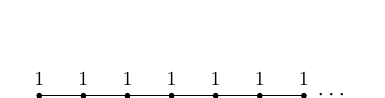
\begin{tikzpicture}[baseline=-.5ex,x=.56cm,y=.56cm]
  \foreach \x in {0,...,6}{
    \fill (\x,0) circle (1.05pt);
    \node[above=1pt,scale=.72] at (\x,0) {$1$};
  }
  \draw (0,0)--(6,0);
  \node[right=2pt,scale=.85] at (6,0) {$\cdots$};
\end{tikzpicture}
\\

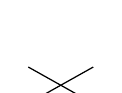
\begin{tikzpicture}[baseline=-.5ex,x=.55cm,y=.55cm]
  \draw[line width=.45pt] (-.75,-.42)--(.75,.42);
  \draw[line width=.45pt] (-.75,.42)--(.75,-.42);
\end{tikzpicture}
& $xy=0$ & $1$ &
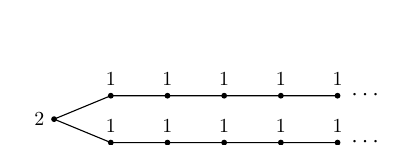
\begin{tikzpicture}[baseline=-.5ex,x=.72cm,y=.62cm]
  \fill (0,0) circle (1.05pt);
  \node[left=1pt,scale=.72] at (0,0) {$2$};
  \foreach \x in {1,...,5}{
    \fill (\x,.48) circle (1.05pt);
    \fill (\x,-.48) circle (1.05pt);
    \node[above=1pt,scale=.72] at (\x,.48) {$1$};
    \node[above=1pt,scale=.72] at (\x,-.48) {$1$};
  }
  \draw (0,0)--(1,.48)--(5,.48);
  \draw (0,0)--(1,-.48)--(5,-.48);
  \node[right=2pt,scale=.85] at (5,.48) {$\cdots$};
  \node[right=2pt,scale=.85] at (5,-.48) {$\cdots$};
\end{tikzpicture}
\\

\begin{tikzpicture}[baseline=-.5ex,x=.55cm,y=.55cm]
  \draw[line width=.45pt] (-.85,0)--(.85,0);
  \draw[line width=.45pt,domain=-.72:.72,samples=40]
    plot (\x,{.72*\x*\x});
\end{tikzpicture}
& $y(y-x^2)=0$ & $2$ &
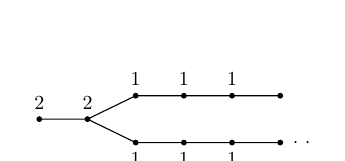
\begin{tikzpicture}[baseline=-.5ex,x=.68cm,y=.62cm]
  \fill (0,0) circle (1.05pt);
  \fill (.9,0) circle (1.05pt);
  \node[above=1pt,scale=.72] at (0,0) {$2$};
  \node[above=1pt,scale=.72] at (.9,0) {$2$};
  \foreach \x/\lab in {1.8/1,2.7/1,3.6/1,4.5/0}{
    \fill (\x,.48) circle (1.05pt);
    \fill (\x,-.48) circle (1.05pt);
    \ifnum\lab=1
      \node[above=1pt,scale=.72] at (\x,.48) {$1$};
      \node[below=1pt,scale=.72] at (\x,-.48) {$1$};
    \fi
  }
  \draw (0,0)--(.9,0)--(1.8,.48)--(4.5,.48);
  \draw (.9,0)--(1.8,-.48)--(4.5,-.48);
  \node[right=2pt,scale=.72] at (4.5,-.48) {$\cdot\ \cdot$};
\end{tikzpicture}
\\

\begin{tikzpicture}[baseline=-.5ex,x=.55cm,y=.55cm]
  \draw[line width=.45pt]
    (0,0) .. controls (.28,.05) and (.55,.35) .. (.72,.78);
  \draw[line width=.45pt]
    (0,0) .. controls (.28,-.05) and (.55,-.35) .. (.72,-.78);
\end{tikzpicture}
& $y^2=x^3$ & $1$ &
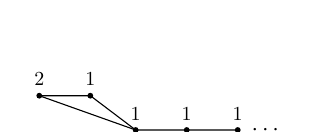
\begin{tikzpicture}[baseline=-.5ex,x=.72cm,y=.65cm]
  \coordinate (A) at (0,.42);
  \coordinate (B) at (.9,.42);
  \coordinate (C) at (1.7,-.25);
  \coordinate (D) at (2.6,-.25);
  \coordinate (E) at (3.5,-.25);
  \foreach \p in {A,B,C,D,E}{\fill (\p) circle (1.05pt);}
  \node[above=1pt,scale=.72] at (A) {$2$};
  \foreach \p in {B,C,D,E}{\node[above=1pt,scale=.72] at (\p) {$1$};}
  \draw (A)--(B)--(C)--(D)--(E);
  \draw (A)--(C);
  \node[right=2pt,scale=.85] at (E) {$\cdots$};
\end{tikzpicture}
\end{tabular}
\end{center}

若 $n>2$，则此图不再确定不变量 $\delta$。例如，三条共点且共面的直线（分别地，不共面的直线）的并，其不变量为 $\delta=3$（分别为 $\delta=2$），而 Enriques 图相同。我不知道这种现象是否也会出现在单支曲线中。

下面给出 $n=3$ 时的两个图的例子，它们不可能由平面曲线产生（参见 2.5）。依次给出曲线的方程、爆破原点后的严格变换的方程、曲线的参数方程、不变量 $\delta$ 和 Enriques 图。

%%%%%%%%%% source scan idx 38 | folio 31 %%%%%%%%%%

\begin{equation}\tag{2.25.1}
\left\{
\begin{gathered}
  \left\{\begin{aligned}y^2&=xz^4,\\ z^3&=x^2,
  \end{aligned}\right.\qquad
  \left\{\begin{aligned}(y/z)^2&=(x/z)^3,\\ z&=(x/z)^2,
  \end{aligned}\right.\\[3pt]
  \left\{\begin{aligned}x&=u^6,\\y&=u^7,\\z&=u^4,
  \end{aligned}\right.\qquad \delta=5
\end{gathered}
\right.
\end{equation}

\begin{center}
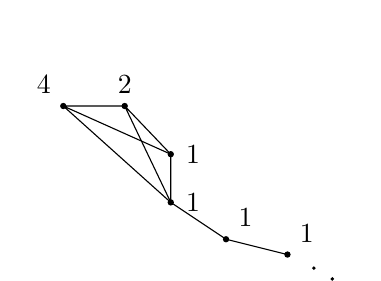
\begin{tikzpicture}[x=.78cm,y=.72cm]
  \coordinate (v1) at (0,0);
  \coordinate (v2) at (1,0);
  \coordinate (v3) at (1.75,-.85);
  \coordinate (v4) at (1.75,-1.70);
  \coordinate (v5) at (2.65,-2.35);
  \coordinate (v6) at (3.65,-2.62);
  \foreach \p in {v1,v2,v3,v4,v5,v6}{\fill (\p) circle (1.15pt);}
  \node[above left=1pt] at (v1) {$4$};
  \node[above=1pt] at (v2) {$2$};
  \node[right=2pt] at (v3) {$1$};
  \node[right=2pt] at (v4) {$1$};
  \node[above right=1pt] at (v5) {$1$};
  \node[above right=1pt] at (v6) {$1$};
  \draw (v1)--(v2) (v1)--(v3) (v1)--(v4);
  \draw (v2)--(v3) (v2)--(v4) (v3)--(v4);
  \draw (v4)--(v5)--(v6);
  \fill (4.08,-2.86) circle (.7pt);
  \fill (4.38,-3.05) circle (.7pt);
  \fill (4.68,-3.24) circle (.7pt);
\end{tikzpicture}
\end{center}

\begin{equation}\tag{2.25.2}
\left\{
\begin{gathered}
  \left\{\begin{aligned}y^2z&=x^3,\\ z^3&=y^2,
  \end{aligned}\right.\qquad
  \left\{\begin{aligned}(y/z)^2&=(x/z)^3,\\ z&=(y/z)^2,
  \end{aligned}\right.\\[3pt]
  \left\{\begin{aligned}x&=u^8,\\y&=u^9,\\z&=u^6,
  \end{aligned}\right.\qquad \delta=10
\end{gathered}
\right.
\end{equation}

\begin{center}
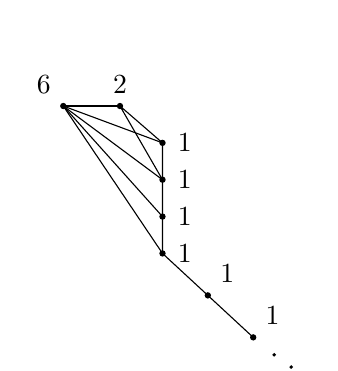
\begin{tikzpicture}[x=.72cm,y=.65cm]
  \coordinate (w1) at (0,0);
  \coordinate (w2) at (1,0);
  \coordinate (w3) at (1.75,-.72);
  \coordinate (w4) at (1.75,-1.44);
  \coordinate (w5) at (1.75,-2.16);
  \coordinate (w6) at (1.75,-2.88);
  \coordinate (w7) at (2.55,-3.70);
  \coordinate (w8) at (3.35,-4.52);
  \foreach \p in {w1,w2,w3,w4,w5,w6,w7,w8}{\fill (\p) circle (1.15pt);}
  \node[above left=1pt] at (w1) {$6$};
  \node[above=1pt] at (w2) {$2$};
  \foreach \p in {w3,w4,w5,w6}{\node[right=2pt] at (\p) {$1$};}
  \node[above right=1pt] at (w7) {$1$};
  \node[above right=1pt] at (w8) {$1$};
  \draw (w1)--(w2);
  \foreach \p in {w3,w4,w5,w6}{\draw (w1)--(\p);}
  \draw (w2)--(w3) (w2)--(w4);
  \draw (w3)--(w4)--(w5)--(w6)--(w7)--(w8);
  \fill (3.72,-4.86) circle (.7pt);
  \fill (4.02,-5.10) circle (.7pt);
  \fill (4.32,-5.34) circle (.7pt);
\end{tikzpicture}
\end{center}

2.26. 下述定理 2.27 在本讲的初版（由 IHES 散发）中曾被表述为一个不正确的猜想。它得益于与 D. S. Rim 的多次讨论，并包含了他的一些结果（D. S. Rim，"Torsion Differentials and Deformations"，定理 2.7(i)）。

%%%%%%%%%% source scan idx 39 | folio 32 %%%%%%%%%%

设 $C$ 是代数闭域 $k$ 上的约化射影曲线，$s\in C(k)$。采用如下记号：

\begin{description}[leftmargin=2.7cm,style=nextline]
\item[$A_s$] $C$ 在 $s$ 处的局部环（或其完备化，这对下文没有影响）；
\item[$\widetilde A_s$] $A_s$ 的正规化；
\item[$\delta(s)$] $\dim_k(\widetilde A_s/A_s)$；
\item[$m_0(s)$] $\operatorname{Spec}(A_s)$ 的形变的完备形式概形 $T$ 的维数。
\end{description}

对 $T$ 的一个不可约分支 $E$，类似地置 $m_0^E(s)=\dim(E)$。

$\widetilde A_s$ 的导子模 $\widetilde\tau$ 及 $A_s$ 的导子模 $\tau$ 均无挠。若 $A_s$ 整，它们嵌入 $A_s$ 的分式域的导子模；一般地，它们嵌入 $A_s$ 的全商环（若干域的积）的导子模。此外，通过这些嵌入，$\tau$ 与 $\widetilde\tau$ 可公度：$\tau/(\tau\cap\widetilde\tau)$ 与 $\widetilde\tau/(\tau\cap\widetilde\tau)$ 在 $k$ 上均为有限维。置

\begin{equation*}
m_1(s)=[\widetilde\tau:\tau]
\mathrel{\mathop=\limits_{\mathrm{def}}}
\dim_k\frac{\widetilde\tau}{\tau\cap\widetilde\tau}
-\dim_k\frac{\tau}{\tau\cap\widetilde\tau}.
\end{equation*}

\underline{定理} 2.27. \underline{设 $E$ 是 $A_s$ 的形变的完备形式概形 $T$ 的一个不可约分支。若 $A_s$ 在 $E$ 的泛点 $e$ 上的形变光滑——也就是说，由 Jacobian 理想定义（VI 5）的、在 $T$ 上有限的形式非光滑子概形的像不包含 $e$——则}

\begin{equation*}
3\delta(s)=m_0^E(s)+m_1(s).
\end{equation*}

%%%%%%%%%% source scan idx 40 | folio 33 %%%%%%%%%%

2.27 的成立与否只依赖于 $A_s$ 的完备化。将 $(C,s)$ 替换为在 $s$ 处与之形式同构的一对 $(C',s)$，可假设下列条件成立：

\begin{enumerate}[label=(\alph*),leftmargin=1.2cm]
\item $s$ 是 $C$ 唯一的奇点；
\item $C$ 没有无穷小自同构。
\end{enumerate}

条件 (b) 保证 $C$ 的形变函子可形式表出。它甚至是有效可形式表出的，因为提升 $C$ 上给定的丰沛可逆层没有障碍。设 $f:X_0\longrightarrow T_0$ 是 $C$ 的万有形变，$t_0$ 是 $T_0$ 的闭点，因而 $C\overset\sim\longrightarrow X_{0t_0}$。

\underline{引理} 2.28. \underline{存在 $k$ 上的有限型概形 $T_1$、点 $t_1\in T_1(k)$ 以及固有平坦态射 $f:X_1\longrightarrow T_1$，其在 $t_1$ 上的纤维为 $C$，使得对每个 $u\in T_1(k)$，$T_1$ 在 $u$ 处的完备化都是纤维 $X_{1u}$ 的形式模概形。}

下面直接证明这个 Artin 一般结果的推论。设 $\mathcal L$ 是 $C$ 上的甚丰沛可逆层，满足 $H^1(C,\mathcal L)=0$，并置 $\mathbb P=\mathbb P(H^0(C,\mathcal L))$。有嵌入 $v:C\hookrightarrow\mathbb P$。设 $T_2$ 是参数化 $\mathbb P$ 中与 $v(C)\subset\mathbb P$ 具有相同 Hilbert 多项式的子簇的 Hilbert 概形，且 $t_2\in T_2$ 对应于 $v(C)$。$T_2$ 在 $t_2$ 处的完备化 $\widehat T_2$ 在 $T_0$ 上光滑。$\widehat T_2/T_0$ 的垂直切丛由 $T_2$ 的切丛的子丛 $L$ 诱导，后者是 $\operatorname{Lie}(\underline{\operatorname{Aut}}(\mathbb P))$ 在 $\underline{\operatorname{Aut}}(\mathbb P)$ 对 $T_2$ 的作用下的像。

在 $t_2$ 的一个邻域中，取方程 $f_1,\ldots,f_n$，其中 $n=\dim\underline{\operatorname{Aut}}(\mathbb P)$，定义 $T_2$ 的一个经过 $t_2$ 的子概形 $T'_1$，且它在 $t_2$ 处的完备化在 $T_0$ 上平展。取 $T_1$ 为 $t_2$ 在 $T'_1$ 中的一个邻域，使其切丛与 $L$ 横截。

%%%%%%%%%% source scan idx 41 | folio 34 %%%%%%%%%%

2.29. 函子态射

\begin{equation*}
(C\text{ 的形变})\longrightarrow(A_s\text{ 的形变})
\end{equation*}

对应于态射 $p:T_0\longrightarrow T$。由 VI 2.10，$p$ 光滑。设 $t$ 是 $T$ 的闭点。$p^{-1}(t)$ 在 $t_0$ 处的 Zariski 切空间分类 $C$ 在 $k[\varepsilon]$ 上的局部平凡形变，其中 $\varepsilon^2=0$。置 $E_0=p^{-1}(E)$，得到

\begin{equation}\tag{2.29.1}
\dim(E_0)=\dim(E)+\dim H^1(C,T^1_{C/k}).
\end{equation}

由于 $X_0/T_0$ 平坦，其所有纤维具有相同的算术亏格 $p$，其中 $1-p=\chi(\underline O)$。根据假设，$E_0$ 的泛点处的纤维光滑。光滑固有曲线的形式模概形光滑且维数为 $3p-3$，故引理 2.28 给出

\begin{equation}\tag{2.29.2}
\dim(E_0)=3p-3.
\end{equation}

设 $\widetilde C$ 是 $C$ 的正规化，其算术亏格为 $\widetilde p=p-\delta(s)$。有

\begin{equation}\tag{2.29.3}
\begin{aligned}
\dim H^1(C,T^1_{C/k})
&=-\chi(C,T^1_{C/k})\\
&=-\chi(\widetilde C,T^1_{\widetilde C/k})+m_1(s)\\
&=[3(p-\delta(s))-3]+m_1(s).
\end{aligned}
\end{equation}

公式（2.29.1）、（2.29.2）和（2.29.3）证明了 2.27。

\underline{猜想} 2.30. \underline{每条约化固有曲线均有光滑形变。}

由 2.27 和 2.28，此猜想蕴含 $A_s$ 的形变的完备形式概形总是等维的，维数为 $3\delta(s)-m_1(s)$。
%%%%%%%%%% source scan idx 42 | folio 35 %%%%%%%%%%

2.31. 设 $C$ 是 $k$ 上算术亏格为 $p$ 的约化固有曲线。采用如下记号：

\begin{description}[leftmargin=2.7cm,style=nextline]
\item[$M_0$] $C$ 的形变的完备形式概形 $T$ 的维数；
\item[$M_1$] $\underline{\operatorname{Aut}}(C)$ 的 Lie 代数的维数。
\end{description}

对 $T$ 的一个不可约分支 $E$，用 $M_0^E$ 表示 $E$ 的维数。2.27 的整体对应结果如下。

\underline{命题} 2.32. \underline{若 $C$ 在 $E$ 的泛点上的形变光滑，则}

\begin{equation*}
3p-3=M_0^E-M_1.
\end{equation*}

设 $X\subset C(k)$ 是 $C$ 的光滑点的一个有限集合，使得 $C$ 上在每个点 $x\in X$ 消失的向量场必为零。$(C,X)$ 的形变函子可形式表出，且满足 2.28 的一个变体。$(C,X)$ 的形式模概形在 $T$ 上光滑，相对维数为 $\#X-M_1$，由 2.28 的类似结果得到

\begin{equation*}
M_0^E+(\#X-M_1)=3p-3+\#X,
\end{equation*}

这就证明了 2.32。

现在假定 $k$ 的\underline{特征为零}。则 $M_1=\dim\underline{\operatorname{Aut}}(C)$。下面给出 $m_1(s)$ 的类似解释。

%%%%%%%%%% source scan idx 43 | folio 36 %%%%%%%%%%

\underline{引理} 2.33. \underline{若 $k$ 的特征为零，则 $A_s$ 的每个导子均可延拓为 $\widetilde A_s$ 的导子。}

若 $D$ 是 $A_s$ 的导子，则

\begin{equation*}
\exp(Dt)=\sum_{n\geq0}\frac{D^nt^n}{n!}
\end{equation*}

是 $A_s\otimes_k k[t]$ 在 $(s,0)$ 处的完备化的自同构。通过结构的搬移，此自同构作用于该环的正规化 $(\widetilde A_s\otimes_k k[t])^{\wedge}$ 上。模 $t^2$ 约化，得到 $\widetilde A_s^{\wedge}\otimes_k k[t]/(t^2)$ 的自同构 $1+Dt$，从而 $D$ 延拓为 $\widetilde A_s^{\wedge}$ 的导子。由于它也可延拓到 $A_s$ 的分式域（当 $A_s$ 不整时则为全商环），所以它可延拓到 $\widetilde A_s$。

假设 $s$ 为奇点。类似的论证表明，由 $D$ 定义的 $\operatorname{Spec}(\widetilde A_s)$ 上的向量场在 $s$ 上方的每一点处消失。

设 $c$ 是 $\widetilde A_s$ 的理想，包含于 $\widetilde A_s/A_s$ 的导子理想中。置

\begin{equation*}
\widetilde G_c=\underline{\operatorname{Aut}}(\widetilde A_s/c),
\end{equation*}

并设 $G_c$ 是 $\widetilde G_c$ 中保持子代数 $A_s/c$ 不变的子群。若 $d\subset c$，则 $\widetilde G_d$ 保持 $c/d$ 不变且满射到 $\widetilde G_c$。注意，对于一致化参数 $t$，$g\in\widetilde G_c$ 由 $g(t)$ 决定，而 $g(t)$ 可以是任意一致化参数。因此，带基点齐性空间 $\widetilde G_c/G_c$ 与 $c$ 无关；将其记为 $\widetilde G/G$。
\begin{editorialnote}
上述关于任意 $d\subset c$ 的不变性断言需要限制。以结点 $A=k[[x,y]]/(xy)$ 为例，其正规化为 $k[[x]]\times k[[y]]$；取 $d=(x^3)\times(y^3)$、$c=(x)\times(y^2)$，则二者都包含于导子，交换两个分支给出模 $d$ 的自同构，却不保持 $c/d$。因此，原书这一论证不能直接用于任意这样的理想。若在完备正规化 $B=\prod_i k[[t_i]]$ 中选用各分支同次幂的理想 $c_N=\prod_i(t_i^N)$，并取 $N_0$ 使 $c_{N_0}$ 包含于导子，则 $N\geq N_0$ 的这些理想在导子内的有限余维理想中共尾。它们是根基的幂，受到全部自同构保持。对 $M\geq N\geq N_0$，截断自同构可以提升一致化参数的系数，故约化映射 $\pi_{MN}:\widetilde G_{c_M}\to\widetilde G_{c_N}$ 为满射。又因 $c_N\subset A$，$A/c_M$ 是 $A/c_N$ 的完整逆像，所以 $\pi_{MN}^{-1}(G_{c_N})=G_{c_M}$；因此对应的齐性商空间在这个受限的共尾系上典范同构。原法文第 36 页也未明写这一限制；此处保留其原论述并注明适用范围。
\end{editorialnote}

设 $\widetilde\tau_0$ 是 $\operatorname{Spec}(\widetilde A_s)$ 上在 $s$ 上方各点处消失的向量场构成的 $\widetilde A_s$-模。当 $s$ 为奇点时，有

\begin{equation*}
\dim_k(\widetilde\tau/\widetilde\tau_0)
=\text{分支数},
\end{equation*}

以及

\begin{equation*}
\widetilde\tau_0/\tau\overset\sim\longrightarrow
\text{商空间 }\widetilde G/G\text{ 在原点的切空间}.
\end{equation*}

%%%%%%%%%% source scan idx 44 | folio 37 %%%%%%%%%%

\underline{命题} 2.34. \underline{在特征零时，若 $s$ 为奇点，则整数 $m_1(s)$ 是分支数与 $\widetilde G/G$ 的维数之和。}

\bigskip
\begin{center}
\underline{\textsc{参考文献}}
\end{center}

\begin{description}[leftmargin=1.1cm,labelwidth=.8cm,labelsep=.3cm]
\item[{[1]}] P. Defrise, \textit{Étude locale des correspondances rationnelles
entre surfaces algébriques}，教授资格论文，Brussels，1949。

\item[{[2]}] P. Deligne 与 D. Mumford, ``The irreducibility of the space of
curves of a given genus,'' \textit{Publ. Math. IHES} \underline{36} (1969),
75--110.

\item[{[3]}] Enriques--Chisini, \textit{Lezioni sulla teoria geometrica delle
equazioni e delle funzioni algebriche}, Zanichelli, Bologna, 1924.

\item[{[4]}] R. Hartshorne, \textit{Residues and Duality}, Lecture Notes in
Mathematics \underline{20}, Springer, 1966.

\item[{[5]}] S. Lichtenbaum, ``Curves over discrete valuation rings,''
\textit{Amer. J. Math.} 90, no. 2（1968 年 4 月）, 380--405.

\item[{[6]}] I. Manin, ``Rational surfaces over perfect fields,''
\textit{Publ. Math. IHES}, no. 30, 55--114.

\item[{[7]}] D. Mumford, ``The topology of normal singularities of an
algebraic surface and a criterion for simplicity,'' \textit{Publ. Math. IHES},
no. 9, 5--22.

\item[{[8]}] A. Néron, \textit{Modèles minimaux des variétés abéliennes sur
les corps locaux et globaux}, Publ. Math., no. 21.

%%%%%%%%%% source scan idx 45 | folio 38 %%%%%%%%%%

\item[{[9]}] M. Raynaud, ``Spécialisation du foncteur de Picard. Critères
numériques de représentabilité,'' \textit{C. R. Acad. Sci. Paris} 264
（1967 年 6 月）, 1001--1004.

\item[{[10]}] Saint-Donat, \textit{Sur un théorème de G. Castelnuovo et
F. Enriques}，第三阶段博士论文，Lyon。

\item[{[11]}] O. Zariski, ``On polynomial ideals defined by infinitely near
base points,'' \textit{Amer. J. Math.} 60 (1938), 151.

\item[{[12]}] D. G. Northcott, ``On the genus formula for plane curves,''
\textit{J. London Math. Soc.} 30 (1955), 376--382.

\item[{[13]}] D. G. Northcott, ``Abstract dilatations and infinitely near
points,'' \textit{Proc. Cambridge Philos. Soc.} 52 (1956), 178--197.

\item[] 关于“无限邻近点”的概念，见下书第二章的 Lipman 附录。

\item[{[14]}] O. Zariski, \textit{Algebraic Surfaces}, Ergebnisse
\underline{61}, Springer-Verlag.
\end{description}

\clearpage
\renewcommand{\CurrentExpose}{第 XI 讲}
\phantomsection\addcontentsline{toc}{section}{第 XI 讲}
\begin{center}\underline{第 XI 讲}\end{center}
\clearpage
\ExposeTOC
\begin{center}
{\large\textbf{SGA 7}}\\[1.5em]
{\Large\underline{第 XI 讲}}\\[2.5em]
{\Large\underline{完全交的上同调}}\\[1.5em]
{\large\underline{P. DELIGNE}}
\end{center}

\bigskip
\noindent\underline{1. 射影空间与完全交的上同调}

设 $X$ 为纯维数为 $n$ 的非奇异复射影簇, $\underline O(1)$ 为 $X$ 上的丰沛可逆层. 根据 Akizuki 与 Nakano [1], Kodaira 消失定理 [4] 蕴含

\begin{equation}\tag{*}
H^i(X,\Omega_X^j(-1))=0\qquad\text{当 }i+j<n.
\end{equation}

仍由 [1], 此结果蕴含复上同调中的``弱 Lefschetz 定理''. 我们拟用直接计算证明: 若 $X$ 是任意特征的域上的射影空间(projective space), 则 (*) 仍成立. 这样, 遵循 [1], 就能把任意特征的域上的完全交(complete intersection)的 Hodge 上同调和 de Rham 上同调与射影空间的相应上同调加以比较.

然后我们将详细说明所得结果的一些推论. 在 §2 中, 我们给出由 Hirzebruch 的数值公式 (2.2) 推出的定性结果. 感谢 N. Katz 在准备该节时给予的帮助.

1.0. 设 $\underline E$ 为概形 $S$ 上秩为 $r+1$ 的局部自由模. \underline{假设 $r>0$.} 回顾 $\mathbb P(\underline E)$ 表示 $\underline E$ 的超平面所组成的 $S$ 上相对射影空间. 设 $p:\mathbb P(\underline E)\to S$ 为投影, 并令

\begin{equation*}
\eta\in H^0\bigl(S,R^1p_*\Omega^1_{\mathbb P(\underline E)/S}\bigr)
\end{equation*}

为可逆层 $\underline O(1)$ 在 Hodge 意义下的第一 Chern 类.

%%%%%%%%%% source scan idx 47 | folio 40 %%%%%%%%%%

回顾 $\eta$ 是 $\underline O(1)$ 在 $H^0(S,R^1p_*\underline O^*)$ 中的类经对数微分

\begin{equation*}
df/f:\underline O^*\longrightarrow
\Omega^1_{\mathbb P(\underline E)/S}.
\end{equation*}

对于 $\mathbb P(\underline E)$ 上任意 $\underline O$-模层 $\underline F$, 令

\begin{equation*}
\underline F(n)=\underline F\otimes\underline O(1)^{\otimes n}
\qquad(n\in\mathbb Z).
\end{equation*}

\underline{定理} 1.1. (i) \underline{层 $R^ip_*(\Omega^j_{\mathbb P(\underline E)/S}(n))$ 局部自由, 且其构造与任意基变换相容.}

(ii) \underline{对于 $0\leq i\leq r$, $R^ip_*(\Omega^i_{\mathbb P(\underline E)/S})$ 的截面 $\eta^i$ 定义了从 $\underline O_S$ 到此层的同构. 此外,}

\begin{equation*}
R^ip_*\Omega^j_{\mathbb P(\underline E)/S}=0
\qquad\underline{\text{若 }}i\ne j\ \underline{\text{ 或 }}\ i>r.
\end{equation*}

(iii) \underline{若 $n\ne0$, 则除下列两种情形外, $R^ip_*(\Omega^j_{\mathbb P(\underline E)/S}(n))$ 均为零:}

\begin{align}
i&=0\quad\underline{\text{且}}\quad n>j,
  \tag{iii$_a$}\\
i&=r\quad\underline{\text{且}}\quad n<j-r.
  \tag{iii$_b$}
\end{align}

设

\begin{equation*}
\mathbb V(\underline E)=\operatorname{Spec}
\bigl(\operatorname{Sym}^*\underline E\bigr)
\end{equation*}

为 $\underline E$ 定义的仿射空间, $e$ 为其零截面, 并令 $\mathbb V(\underline E)^*=\mathbb V(\underline E)\setminus e(S)$. 设 $a$ 和 $a'$ 分别为 $\mathbb V(\underline E)$ 和 $\mathbb V(\underline E)^*$ 到 $S$ 的投影, $q$ 为 $\mathbb V(\underline E)^*$ 到 $\mathbb P(\underline E)$ 的投影:

\begin{center}
\begin{tikzcd}[row sep=large,column sep=large]
\mathbb V(\underline E)
  \arrow[dr,"a"]
& \mathbb V(\underline E)^*
  \arrow[l,hook']
  \arrow[r,"q"]
  \arrow[d,"a'"']
& \mathbb P(\underline E)
  \arrow[dl,"p"]
\\
{} & S\arrow[ul,bend right,"e"'] & {}
\end{tikzcd}
\qquad .
\end{center}

$\mathbb P(\underline E)$ 上的去零截面仿射空间 $\mathbb V(\underline O(1))^*$ 与 $\mathbb V(\underline E)^*$ 典范同构. 因此, 对于 $\mathbb P(\underline E)$ 上任意拟凝聚 $\underline O$-模层 $\underline F$, 存在典范同构

%%%%%%%%%% source scan idx 48 | folio 41 %%%%%%%%%%

\begin{equation}\tag{1.1.1}
q_*q^*\underline F\simeq
\bigoplus_{n\in\mathbb Z}\underline F(n).
\end{equation}

$q_*q^*\underline F$ 的这个分次也可以由 $\mathbb V(\underline E)$ 的位似群 $\mathbb G_m$ 在此层上的作用得到.

$\mathbb V(\underline E)$ 上的相对向量场可等同于 $\mathbb V(\underline E)$ 到自身的 $S$-态射, 其中将目标视为原点处的切空间. 由 $\mathbb V(\underline E)$ 的恒等映射定义的向量场 $X$ 在位似下不变. 它与 $q$ 的纤维相切, 并定义了一个平凡化

\begin{equation}\tag{1.1.2}
X:\Omega^1_{\mathbb V(\underline E)^*/\mathbb P(\underline E)}
\longrightarrow\underline O_{\mathbb V(\underline E)^*}.
\end{equation}

若 $x_i$ 构成 $\underline E$ 的一组基, 则

\begin{equation*}
X=\sum_i x_i\,dx^i.
\end{equation*}

由于 $\Omega^1_{\mathbb V(\underline E)^*/\mathbb P(\underline E)}$ 的秩为一, 正合列

\begin{equation*}
0\longrightarrow q^*\Omega^1_{\mathbb P(\underline E)/S}
\longrightarrow\Omega^1_{\mathbb V(\underline E)^*/S}
\longrightarrow
\Omega^1_{\mathbb V(\underline E)^*/\mathbb P(\underline E)}
\longrightarrow0
\end{equation*}

诱导正合列

\begin{equation*}
0\longrightarrow q^*\Omega^i_{\mathbb P(\underline E)/S}
\longrightarrow\Omega^i_{\mathbb V(\underline E)^*/S}
\longrightarrow
\Omega^1_{\mathbb V(\underline E)^*/\mathbb P(\underline E)}
\otimes q^*\Omega^{i-1}_{\mathbb P(\underline E)/S}
\longrightarrow0.
\end{equation*}

利用 (1.1.2), 它们变为

\begin{equation}\tag{1.1.3}
0\longrightarrow q^*\Omega^i_{\mathbb P(\underline E)/S}
\longrightarrow\Omega^i_{\mathbb V(\underline E)^*/S}
\xrightarrow{\ \iota_X\ }
q^*\Omega^{i-1}_{\mathbb P(\underline E)/S}
\longrightarrow0.
\end{equation}

典范地有

\begin{equation}\tag{1.1.4}
\Omega^i_{\mathbb V(\underline E)/S}
=a^*\bigwedge^i\underline E.
\end{equation}

所以短正合列 (1.1.3) 由 $\mathbb V(\underline E)^*$ 上的下列长正合列分解而成:

\begin{equation}\tag{1.1.5}
\cdots\longrightarrow {a'}^*\bigwedge^i\underline E
\xrightarrow{\ \iota_X\ }
{a'}^*\bigwedge^{i-1}\underline E
\xrightarrow{\ \iota_X\ }
{a'}^*\bigwedge^{i-2}\underline E\longrightarrow\cdots.
\end{equation}


这个长正合列就是 $\mathbb V(\underline E)$ 上 $\underline O_{e(S)}$ 的 Koszul 解消在 $\mathbb V(\underline E)^*$ 上的限制.

经仿射态射 $q$ 将长正合列 (1.1.5) 直像到 $\mathbb P(\underline E)$. 由 (1.1.1) 和公式 $q_*{a'}^*=q_*q^*p^*$, 得到长正合列

\begin{equation}\tag{1.1.6}
\cdots\longrightarrow
\bigoplus_{n\in\mathbb Z}p^*\bigwedge^i\underline E(n)
\xrightarrow{\ \iota_X\ }
\bigoplus_{n\in\mathbb Z}p^*\bigwedge^{i-1}\underline E(n)
\longrightarrow\cdots .
\end{equation}

它分解为短正合列, 即 (1.1.3) 的像,

\begin{equation}\tag{1.1.7}
0\longrightarrow
\bigoplus_{n\in\mathbb Z}\Omega^i_{\mathbb P(\underline E)/S}(n)
\longrightarrow
\bigoplus_{n\in\mathbb Z}p^*\bigwedge^i\underline E(n)
\xrightarrow{\ \iota_X\ }
\bigoplus_{n\in\mathbb Z}\Omega^{i-1}_{\mathbb P(\underline E)/S}(n)
\longrightarrow0.
\end{equation}

正合列 (1.1.7) 是下列正合列的直和

\begin{equation}\tag{1.1.8}
0\longrightarrow\Omega^i_{\mathbb P(\underline E)/S}(n)
\longrightarrow p^*\bigwedge^i\underline E(n-i)
\xrightarrow{\ \iota_X\ }
\Omega^{i-1}_{\mathbb P(\underline E)/S}(n)
\longrightarrow0.
\end{equation}

回顾 (EGA III, 2.1.15, 或 FAC), 层 $R^ip_*\underline O(k)$ 局部自由, 其构造与任意基变换相容, 且

\begin{equation}\tag{1.1.9}
R^ip_*\underline O(k)=0
\quad\text{若 }i\ne0,r,
\quad\text{或若 }i=0, k<0,
\quad\text{或若 }i=r, k>-r-1,
\end{equation}

因而 $R^ip_*p^*\bigwedge^j\underline E(k)$ 在相同条件下为零.

正合列 (1.1.8) 给出 $\Omega^i_{\mathbb P(\underline E)/S}(n)$ 的解消

\begin{equation}\tag{1.1.10}
0\longrightarrow\Omega^i_{\mathbb P(\underline E)/S}(n)
\xrightarrow{\ E\ }p^*\bigwedge^i\underline E(n-i)
\xrightarrow{\ \iota_X\ }\cdots\longrightarrow
p^*\bigwedge^0\underline E(n)\longrightarrow0
\end{equation}

由 (1.1.9), 这个解消定义的谱序列由于次数的原因而退化 ($E_1=E_\infty$); 对 $0<j<r$, 它给出

\begin{equation}\tag{1.1.11}
R^jp_*\Omega^i_{\mathbb P(\underline E)/S}(n)
=\mathcal H\left(\cdots\xrightarrow{\ \iota_X\ }
p_*\bigwedge^{i-j}\underline E(n-i+j)
\xrightarrow{\ \iota_X\ }\cdots\right).
\end{equation}

由于 $r\geq1$, 由深度论证可知

\begin{equation}\tag{1.1.12}
\bigoplus_{n\in\mathbb Z}p_*p^*\bigwedge^i\underline E(n)
=p_*q_*q^*p^*\bigwedge^i\underline E
={a'}_*{a'}^*\bigwedge^i\underline E
=a_*a^*\bigwedge^i\underline E.
\end{equation}

%%%%%%%%%% source scan idx 50 | folio 43 %%%%%%%%%%

于是 $p_*p^*\bigwedge^i\underline E(n)$ 是 $a_*a^*\bigwedge^i\underline E$ 中权为 $n+i$ 的齐次部分, 即 $\operatorname{Sym}^n(\underline E)\otimes\bigwedge^i\underline E$. 考虑到 (1.1.5) 来自 Koszul 解消, (1.1.11) 表明: 对 $0<j<r$, 层 $R^jp_*\Omega^i_{\mathbb P(\underline E)/S}(n)$ 只有在 $i-j=0$ 且 $n-i+j=0$, 即 $n=0$ 且 $i=j$ 时才可能非零. 此外, 在此情形下, $R^ip_*\Omega^i_{\mathbb P(\underline E)/S}$ 同构于 $\underline O_S$.

对于 $j=0$, (1.1.10) 还给出

\begin{equation}\tag{1.1.13}
p_*\Omega^i_{\mathbb P(\underline E)/S}(n)
=\ker\!\left(\iota_X:
p_*\bigwedge^i\underline E(n-i)\longrightarrow
p_*\bigwedge^{i-1}\underline E(n-i+1)\right),
\end{equation}

同一论证表明, 当 $n-i\leq0$ 时 $\iota_X$ 为单射.

在 (1.1.8) 中取 $n=0$ 和 $i=r+1$, 得到

\begin{equation*}
\Omega^r_{\mathbb P(\underline E)/S}\simeq
p^*\bigwedge^{r+1}\underline E(-r-1).
\end{equation*}

当 $S$ 为域的谱时, 1.1(ii) 和 (iii) 中的消失断言在 $j\ne r$ 时由上述论证得到, 在 $j=r$ 时则通过对偶性 ([2], V, 11.2, 第~211 页) 从上述论证得到. 特别地, 对任意 $j$ 和 $n$, 至多有一个 $i$ 使 $R^ip_*\Omega^j_{\mathbb P(\underline E)/S}(n)\ne0$. 由于 $\Omega^j_{\mathbb P(\underline E)/S}$ 在 $S$ 上平坦, 这就证明了 (i) (最困难的是在 EGA III 中找到出处; 我们建议使用 6.10.5, 7.4.1 和 7.5.5, 然后取极限).

已知对 $0\leq i\leq r$, $R^ip_*\Omega^i_{\mathbb P(\underline E)/S}$ 为可逆层, 只须证明当 $S$ 为域的谱时 $\eta^i\ne0$. 实际上, $\eta^r$ 是一个有理点 (即 $r$ 个超平面的交) 的上同调类, 因而是 $H^r(\mathbb P^r,\Omega^r)$ 的一组基 (FGA, 第 149 讲, 第~4 节).

1.2. $\Omega^i(n)$ 的 Euler--Poincaré 示性数可以直接用 (1.1.10) 或 (1.1.13) 计算. 其结果虽不甚悦目, 却是

\begin{equation*}
\chi\bigl(\mathbb P^r_k,\Omega^j_{\mathbb P^r_k}(n)\bigr)
=\sum_{0\leq i\leq j}(-1)^{i-j}
\binom{r+1}{i}\binom{r+n-i}{r}.
\end{equation*}


%%%%%%%%%% source scan idx 51 | folio 44 %%%%%%%%%%

\underline{命题} 1.3. \underline{设 $f:X\to S$ 为固有光滑态射, $\underline W$ 为 $X$ 上秩为 $c$ 的局部自由层, $\underline F$ 为 $X$ 上的凝聚层, $d>0$ 为整数, $s:\underline W\to\underline O_X$ 为 $\underline W^\vee$ 的截面. 假设 $S$ 为诺特概形, 且满足:}

\begin{enumerate}[label=(\alph*),leftmargin=2.4em]
\item \underline{由 $s$ 的零点定义的 $X$ 的闭子概形 $H$ 在 $S$ 上光滑.}

\item \underline{在 $X$ 上局部地, 若 $s_i$ 为 $s$ 在 $\underline W^\vee$ 的一组基下的坐标, 则 $s_i$ 既为 $\underline O_X$-正则序列, 也为 $\underline F$-正则序列.}

\item \underline{对每个不全为零的整数序列 $k_\ell$, 都有}
\end{enumerate}

\begin{equation*}
R^if_*\left(\bigotimes_\ell\bigwedge^{k_\ell}\underline W
\otimes\Omega^j_{X/S}\otimes\underline F\right)=0
\qquad\underline{\text{当 }}i+j<d.
\end{equation*}

\underline{则:}

\begin{align*}
R^if_*\left(\Omega^j_{X/S}\otimes\underline F\right)
&\xrightarrow{\ \sim\ }
R^if_*\left(\Omega^j_{H/S}\otimes\underline F\right)
&&\underline{\text{当 }}i+j<d-c, \tag{i}\\
R^if_*\left(\Omega^j_{X/S}\otimes\underline F\right)
&\lhook\joinrel\longrightarrow
R^if_*\left(\Omega^j_{H/S}\otimes\underline F\right)
&&\underline{\text{当 }}i+j=d-c. \tag{ii}
\end{align*}

$H$ 在 $X$ 中的余法层 $N_{H/X}$ 同构于 $\underline W$ 在 $H$ 上的限制, 所以正合列

\begin{equation}\tag{1.3.1}
0\longrightarrow N_{H/X}\longrightarrow
\Omega^1_{X/S}\otimes\underline O_H\longrightarrow
\Omega^1_{H/S}\longrightarrow0
\end{equation}

在 $\Omega^j_{X/S}\otimes\underline O_H$ 上定义递减滤过, 其相继商为

\begin{equation}\tag{1.3.2}
\operatorname{Gr}^k\bigl(\Omega^j_{X/S}\otimes\underline O_H\bigr)
\simeq\bigwedge^k\underline W\otimes\Omega^{j-k}_{H/S}.
\end{equation}

由 (b) 还可得到

\begin{equation}\tag{1.3.3}
\operatorname{Gr}^k\bigl(\Omega^j_{X/S}\otimes\underline O_H
\otimes\underline F\bigr)
=\bigwedge^k\underline W\otimes\Omega^{j-k}_{H/S}
\otimes\underline F.
\end{equation}

我们对 $j$ 归纳, 同时对所有满足 (b) 和 (c) 的 $\underline F$ 证明 (i) 和 (ii). 当 $j<0$ 时, 两断言均为空断言.

%%%%%%%%%% source scan idx 52 | folio 45 %%%%%%%%%%

于是, 假定对于 $j'<j$ 已证明 (i) 和 (ii). 归纳假设适用于层 $\bigwedge^k\underline W\otimes\underline F$, 由 (c) 得到

\begin{equation}\tag{1.3.4}
R^if_*\left(\bigwedge^k\underline W\otimes
\Omega^{j-k}_{H/S}\otimes\underline F\right)=0
\quad\text{当 }k>0\text{ 且 }i+j<d-c+k.
\end{equation}

上面所考虑的 $\Omega^j_{X/S}\otimes\underline O_H\otimes\underline F$ 的滤过定义了谱序列

\begin{equation*}
E_1^{p,i-p}=R^if_*\left(\bigwedge^p\underline W\otimes
\Omega^{j-p}_{H/S}\otimes\underline F\right)
\Longrightarrow
R^if_*\left(\Omega^j_{X/S}\otimes\underline O_H
\otimes\underline F\right).
\end{equation*}

由 (1.3.4), 当 $p>0$ 且 $i+j\leq d-c$ 时 $E_1^{p,i-p}=0$; 因而

\begin{equation}\tag{1.3.5}
\left\{
\begin{aligned}
R^if_*\left(\Omega^j_{X/S}\otimes\underline O_H\otimes\underline F\right)
&\xrightarrow{\ \sim\ }
R^if_*\left(\Omega^j_{H/S}\otimes\underline F\right)
&&\text{若 }i+j<d-c,\\
R^if_*\left(\Omega^j_{X/S}\otimes\underline O_H\otimes\underline F\right)
&\lhook\joinrel\longrightarrow
R^if_*\left(\Omega^j_{H/S}\otimes\underline F\right)
&&\text{若 }i+j=d-c.
\end{aligned}
\right.
\end{equation}

由假设 (b), 赋予适当微分后, 层 $\bigwedge^k\underline W\otimes\Omega^j_{X/S}\otimes\underline F$ 构成 $\Omega^j_{X/S}\otimes\underline O_H\otimes\underline F$ 的左 Koszul 解消. 这个滤过定义了谱序列

\begin{equation}\tag{1.3.6}
E_1^{-p,q}=R^qf_*\left(\bigwedge^p\underline W\otimes
\Omega^j_{X/S}\otimes\underline F\right)
\Longrightarrow
R^{q-p}f_*\left(\Omega^j_{X/S}\otimes\underline O_H
\otimes\underline F\right).
\end{equation}

由假设 (c), 当 $p>0$ 且 $q+j<d$ 时 $E_1^{-p,q}=0$; 当 $p\notin[0,c]$ 时显然也为零. 因此,

\begin{equation}\tag{1.3.7}
\left\{
\begin{aligned}
R^if_*\left(\Omega^j_{X/S}\otimes\underline F\right)
&\xrightarrow{\ \sim\ }
R^if_*\left(\Omega^j_{X/S}\otimes\underline O_H\otimes\underline F\right)
&&\text{若 }i+j<d-c,\\
R^if_*\left(\Omega^j_{X/S}\otimes\underline F\right)
&\lhook\joinrel\longrightarrow
R^if_*\left(\Omega^j_{X/S}\otimes\underline O_H\otimes\underline F\right)
&&\text{若 }i+j=d-c.
\end{aligned}
\right.
\end{equation}
\EditorialFootnote{法文原印本与英文底本在 (1.3.7) 右侧均写作 $R^if_*(\Omega^j_{H/S}\otimes\underline F)$. 由 (1.3.6) 的收敛项, 此处应为 $R^if_*(\Omega^j_{X/S}\otimes\underline O_H\otimes\underline F)$; 再与 (1.3.5) 合成即得结论.}

现在由 (1.3.5) 和 (1.3.7) 即得断言 (i) 和 (ii).


%%%%%%%%%% source scan idx 53 | folio 46 %%%%%%%%%%

1.4. 设 $\underline E$ 为概形 $S$ 上秩为 $r+1$ 的局部自由层, $\mathbb P(\underline E)$ 为相应的射影丛, $d\leq r$ 为整数, $\underline a=(a_1,\ldots,a_d)$ 为整数序列. $\mathbb P(\underline E)$ 中多重次数为 $\underline a$ 的相对\underline{完全交}, 是指在每个纤维中余维均为 $d$ 的闭子概形, 且在 $S$ 的平展拓扑下局部地是次数分别为 $a_1,\ldots,a_d$ 的 $d$ 个超曲面的交.

由 1.1, 对于 $X/S=\mathbb P(\underline E)/S$, $\underline F=\underline O_X$,

\begin{equation*}
\underline W=\bigoplus_i\underline O(-a_i),
\end{equation*}

以及定义多重次数为 $\underline a$ 的相对完全交 $Y\subset\mathbb P(\underline E)$ 的 $\underline W^\vee$ 的截面 $s$, 1.3 的假设 (b) 和 (c) 成立.

\underline{定理} 1.5. \underline{在 1.4 的假设下, 设 $n=r-d$ 为 $Y$ 的相对维数, $\eta\in H^0(S,R^1f_*\Omega^1_{Y/S})$ 为下图中 $\underline O(1)$ 的第一 Chern 类}

\begin{center}
\begin{tikzcd}[column sep=large,row sep=large]
Y\arrow[rr,hook]\arrow[dr,dash,"f"']&&
\mathbb P(\underline E)\arrow[dl,"g"]\\
&S&{}
\end{tikzcd}
\qquad .
\end{center}

\underline{若 $Y$ 在 $S$ 上光滑, 则:}

\begin{enumerate}[label=(\roman*),leftmargin=2.6em]
\item \underline{层 $R^if_*\Omega^j_{Y/S}$ 局部自由, 且其构造与任意基变换相容.}

\item \underline{联系 Hodge 上同调与 de Rham 上同调的谱序列}
\begin{equation*}
E_1^{p,q}=R^qf_*\Omega^p_{Y/S}\Longrightarrow
R^{p+q}f_*(\Omega^*_{Y/S}),
\end{equation*}
\underline{退化 ($E_1=E_\infty$); 其极限局部自由, 且其构造与任意基变换相容.}
\end{enumerate}

\noindent(iii)$_a$ \underline{有}

\begin{equation*}
R^if_*\Omega^j_{Y/S}=0
\qquad\underline{\text{若 }}i\ne j\ \underline{\text{ 且 }}\ i+j\ne n.
\end{equation*}

%%%%%%%%%% source scan idx 54 | folio 47 %%%%%%%%%%

\noindent(iii)$_b$ \underline{若 $2i<n$, 则 $\eta^i$ 为 $R^if_*\Omega^i_{Y/S}$ 的一组基.}

\noindent(iii)$_c$ \underline{若 $n<2i\leq2n$, 且 $\alpha_i$ 为 $R^if_*\Omega^i_{Y/S}$ 中与 $R^{n-i}f_*\Omega^{n-i}_{Y/S}$ 的基 $\eta^{n-i}$ 对偶的基, 则}

\begin{equation*}
\eta^i=\left(\prod_{h=1}^d a_h\right)\alpha_i.
\end{equation*}

\noindent(iii)$_d$ \underline{若 $n=2m$, 则 $\eta^m\ne0$ (只要 $S\ne\varnothing$), 且商 $R^mf_*\Omega^m_{Y/S}/\underline O_S\eta^m$ 局部自由.}

只须在``普遍''情形下证明 1.5, 这使我们可以假设 $S$ 在 $\operatorname{Spec}(\mathbb Z)$ 上光滑. 此时 (ii) 由 (i) 得到, 因为由 Hodge 理论, (ii) 在 $\mathbb C$ 上成立, 从而在每个零特征域上成立. 此外, 由于 $S$ 为约化概形, 若假定在 $S$ 为域的谱时已证明 (iii), 则 (i) 由 (iii) 得到. 事实上, 由 (iii), 对每个 $j$, 函数

\begin{equation*}
s\longmapsto\dim_{k(s)}H^i(Y_s,\Omega^j_{Y_s})
\end{equation*}

在 $S$ 上均为常数, 至多 $i+j=n$ 时例外\EditorialFootnote{法文原印本与英文底本此处均写作 $i=j$. 由 (iii)$_a$--(iii)$_c$, 对固定的 $j$, 唯一尚待确定的维数项是 $i+j=n$ 的中间上同调项.}; 因其交错和为常数 (EGA III, 7.9.2), 故它们全都为常数. 再由 EGA III, 6.10.5, 7.6.9 和 7.7.5 即得结论.

由 1.4 和 1.3, 有

\begin{equation}\tag{1.5.1}
\left\{
\begin{aligned}
R^ig_*\Omega^j_{\mathbb P(\underline E)/S}
&\xrightarrow{\ \sim\ }R^if_*\Omega^j_{Y/S}
&&\text{当 }i+j<n,\\
R^ig_*\Omega^j_{\mathbb P(\underline E)/S}
&\lhook\joinrel\longrightarrow R^if_*\Omega^j_{Y/S}
&&\text{当 }i+j=n.
\end{aligned}
\right.
\end{equation}

当 $S$ 为域的谱时, 断言 (iii)$_a$, (iii)$_b$ 和 (iii)$_d$ 由 (1.5.1) 与 Serre 对偶性 ([2], V, 11.2, 第~211 页) 得到. 上同调类

%%%%%%%%%% source scan idx 55 | folio 48 %%%%%%%%%%

$\eta^n$ 是次数为 $\prod_{h=1}^d a_h$ (即完全交的次数) 的零圈的类, 所以

\begin{equation*}
\eta^n=\left(\prod_{h=1}^d a_h\right)\alpha_n.
\end{equation*}

根据定义, $\eta^{n-i}\alpha_i=\alpha_n$, 从而得到 (iii)$_c$.

于是 (i) 和 (ii) 成立; 在普遍情形下, (iii) 中各断言由 (i) 和已经证明的 $S$ 为域的谱时的 (iii) 得到.

\underline{定理} 1.6. \underline{保留 1.4 和 1.5 的假设与记号, 假定 $Y$ 光滑, 设 $\ell$ 为在 $S$ 的所有剩余域中可逆的素数, 并以 $\eta_\ell\in H^0(S,R^2f_*\mathbb Z_\ell(1))$ 表示 $\underline O(1)$ 的 $\ell$ 进第一 Chern 类 (SGA 5, VII). 则:}

\begin{enumerate}[label=(\roman*),leftmargin=2.6em]
\item \underline{若 $i$ 为奇数且 $i\ne n$, 则 $R^if_*\mathbb Z_\ell=0$.}

\item \underline{若 $2i<n$, 则 $R^{2i}f_*\mathbb Z_\ell(i)$ 同构于 $\mathbb Z_\ell$, 并以 $\eta_\ell^i$ 为基.}

\item \underline{若 $n<2i\leq2n$, 则 $R^{2i}f_*\mathbb Z_\ell(i)$ 同构于 $\mathbb Z_\ell$, 并以}
\begin{equation*}
\eta_\ell^i\bigg/\prod_{h=1}^d a_h
\end{equation*}
\underline{为基.}

\item \underline{$\mathbb Z_\ell$-层 $R^nf_*\mathbb Z_\ell$ 可构造、扭常且无挠. 若 $n$ 为偶数, 则 $\eta_\ell^{n/2}\ne0$ (只要 $S\ne\varnothing$), 且 $R^nf_*\mathbb Z_\ell(n/2)/\mathbb Z_\ell\eta_\ell^{n/2}$ 无挠.}
\end{enumerate}

由 SGA 4, XVI, 2.2, $\mathbb Z_\ell$-层 $R^if_*\mathbb Z_\ell$ 可构造且扭常, 其构造与任意基变换相容. 因此, 只须在 $S$ 为代数闭域的谱时证明 1.6. 此时反复应用 SGA 4, XIV, 3.3 可知, 对每个 $m$, 典范映射

\begin{equation*}
H_Y^q\bigl(\mathbb P(\underline E),\mathbb Z/\ell^m\bigr)
\longrightarrow H^q(Y,\mathbb Z/\ell^m)
\end{equation*}

%%%%%%%%%% source scan idx 56 | folio 49 %%%%%%%%%%

当 $q>r+d$ 时为双射, 当 $q=r+d$ 时为满射. 由此和 Poincaré 对偶性 (SGA 4, XVIII), 推得 (SGA 5, VII) 限制映射

\begin{equation*}
H^q\bigl(\mathbb P(\underline E),\mathbb Z_\ell\bigr)
\longrightarrow H^q(Y,\mathbb Z_\ell)
\end{equation*}

当 $q<n$ 时为双射, 当 $q=n$ 时为单射且余核无挠. 这证明了 $i<n$ 时的 (i), 以及 (ii) 和 (iv). 与 1.5 中相同, 可验证 $\eta_\ell^n$ 是典范类的 $\prod_{h=1}^d a_h$ 倍; 再由 Poincaré 对偶性 (SGA 4, XVIII) 得到 (i) 和 (iii).


1.7. 若 $Y$ 为域 $k$ 上的射影空间 $\mathbb P^r(k)$ 中维数至少为三的完全交, 则已知 $\operatorname{Pic}(Y)$ 同构于 $\mathbb Z$, 并由 $\underline O(1)$ 生成 (SGA 2, XII, 3.7). 在二维时, 若 $Y$ 光滑, 仍可证明如下结果.

\underline{定理} 1.8. \underline{设 $Y$ 为代数闭域 $k$ 上射影空间 $\mathbb P^r(k)$ 中的光滑完全交曲面. 则 $\underline{\operatorname{Pic}}^\tau(Y)=0$, 且 $\underline O(1)$ 的类在 Néron--Severi 群 $\operatorname{NS}(Y)$ 中不可除.}

由 1.5(iii)$_a$ 知 $H^1(Y,\underline O)=0$, 因而 $\underline{\operatorname{Pic}}^0(Y)=0$. 再由下面的熟知引理、1.6(iv) 所保证的 $H^2(Y,\mathbb Z_\ell(1))$ 无挠性, 以及 1.5(iii)$_a$ 给出的 $H^0(Y,\Omega_Y^1)=0$, 即得 $\underline{\operatorname{Pic}}^\tau(Y)$ 为零.

\underline{引理} 1.9. \underline{设 $Y$ 为代数闭域 $k$ 上的完备代数簇.}

\begin{enumerate}[label=(\roman*),leftmargin=2.6em]
\item \underline{若 $\ell$ 与 $k$ 的特征互素, 则 $\operatorname{NS}(Y)$ 的 $\ell$ 挠子群可等同于 $H^2(Y,\mathbb Z_\ell(1))$ 的 $\ell$ 挠子群.}

%%%%%%%%%% source scan idx 57 | folio 50 %%%%%%%%%%

\item \underline{若 $k$ 的特征 $p$ 非零且 $Y$ 光滑, 则 $\operatorname{Pic}(Y)$ 中乘以 $p$ 的核可等同于 $H^0(Y,\Omega_Y^1)$ 中由局部对数微分组成的子群.}
\end{enumerate}

Kummer 正合列

\begin{equation*}
0\longrightarrow\mu_{\ell^n}\longrightarrow\mathbb G_m
\xrightarrow{\ x\mapsto x^{\ell^n}\ }\mathbb G_m\longrightarrow0
\end{equation*}

给出正合列

\begin{equation*}
0\longrightarrow
\operatorname{Pic}(Y)/\ell^n\operatorname{Pic}(Y)
\longrightarrow H^2(Y,\mu_{\ell^n})
\longrightarrow H^2(Y,\mathbb G_m)_{\ell^n}
\longrightarrow0,
\end{equation*}

其中

\begin{equation*}
\operatorname{Pic}(Y)/\ell^n\operatorname{Pic}(Y)
=\operatorname{NS}(Y)\otimes\mathbb Z/\ell^n.
\end{equation*}

取逆极限得到

\begin{equation*}
0\longrightarrow\operatorname{NS}(Y)\otimes\mathbb Z_\ell
\longrightarrow H^2(Y,\mathbb Z_\ell(1))
\longrightarrow
\operatorname{Hom}\bigl(\mathbb Q_\ell/\mathbb Z_\ell,
H^2(Y,\mathbb G_m)\bigr)
\longrightarrow0.
\end{equation*}

由于 $\mathbb Q_\ell/\mathbb Z_\ell$ 可除, 余核无挠. 这就证明了 (i).

为证明 (ii), 只须注意正合列

\begin{equation*}
0\longrightarrow\underline O_Y^*
\xrightarrow{\ x\mapsto x^p\ }\underline O_Y^*
\xrightarrow{\ df/f\ }\Omega_Y^1
\end{equation*}

定义了短正合列

\begin{equation*}
0\longrightarrow\underline O_Y^*\longrightarrow\underline O_Y^*
\longrightarrow\Omega^1_{Y,\mathrm{loc}\,\log}\longrightarrow0,
\end{equation*}

再取相应的上同调长正合列即可. 此论证出自 Cartier; 他还证明, 若以 $C$ 表示 $H^0(Y,\Omega_Y^1)$ 上的 Cartier 算子, 则局部对数微分构成 $C-\operatorname{Id}$ 的核.

反设 $\underline O(1)$ 在 $\operatorname{NS}(Y)$ 中的类具有形式 $nu$, 其中 $n>1$. 若 $\ell$ 整除 $n$ 且与特征互素, 则在 $\ell$ 进上同调中仍有

%%%%%%%%%% source scan idx 58 | folio 51 %%%%%%%%%%

\begin{equation*}
\eta_\ell=n\,c_1(u),
\end{equation*}

这与 1.6(iv) 矛盾.

最后, 若 $k$ 的特征 $p$ 非零且 $p$ 整除 $n$, 则在 Hodge 上同调中仍有

\begin{equation*}
\eta=n\,c_1(u)=0,
\end{equation*}

这与 1.5(iii)$_d$ 矛盾, 证明完毕.


2. \underline{数值结果}

2.1. 设 $\underline a=(a_i)_{1\leq i\leq d}$ 为由 $\geq1$ 的整数构成的序列, $V_n(\underline a)$ 表示域 $k$ 上射影空间 $\mathbb P^{n+d}$ 中维数为 $n$、多重次数为 $\underline a$ 的光滑完全交. 令

\begin{equation*}
h^{p,q}(\underline a)
=\dim_k H^q\bigl(V_{p+q}(\underline a),\Omega^p\bigr)
\end{equation*}

以及

\begin{equation*}
h_0^{p,q}(\underline a)=h^{p,q}(\underline a)-\delta_{p,q}.
\end{equation*}

于是 $h_0^{p,q}(\underline a)$ 是多重次数为 $\underline a$ 的完全交的中间维本原上同调的 Hodge 数. 由 1.5, 它们只依赖于 $\underline a$, $p$ 和 $q$. 置

\begin{equation}\tag{2.1.1}
H(\underline a)=\sum_{p,q\geq0}h_0^{p,q}(\underline a)y^pz^q
\in\mathbb Z[[y,z]].
\end{equation}

当 $d=1$ 且 $\underline a=(a)$ 时, 置 $h^{p,q}(a)=h^{p,q}(\underline a)$ 和 $H(a)=H(\underline a)$. 当 $d=0$ 时, 置 $\sup(a_i)=1$.

以下公式是 Hirzebruch [3] 第~160 页公式 (2) 在 $k=0$ 时的特例:

%%%%%%%%%% source scan idx 59 | folio 52 %%%%%%%%%%

\begin{equation}\tag{2.2}
\sum_{n=0}^{\infty}\sum_p
\chi\bigl(V_n(\underline a),\Omega^p\bigr)y^pz^{n+d}
=\frac{1}{(1+yz)(1-z)}
\prod_{i=1}^d
\frac{(1+yz)^{a_i}-(1-z)^{a_i}}
{(1+yz)^{a_i}z+y(1-z)^{a_i}}.
\end{equation}

我们将其变换为如下公式.

\underline{定理} 2.3 (Hirzebruch). \underline{沿用 2.1 的记号, 有}

\begin{equation*}
H(\underline a)=\frac{1}{(1+y)(1+z)}\left[
\prod_{i=1}^d
\frac{(1+y)^{a_i}-(1+z)^{a_i}}
{-(1+y)^{a_i}z+(1+z)^{a_i}y}-1\right].
\end{equation*}

由 1.5,

\begin{equation*}
\chi\bigl(V_n(\underline a),\Omega^p\bigr)
=(-1)^p+(-1)^{n-p}h_0^{p,n-p}(\underline a).
\end{equation*}

因此, (2.2) 的左端 $I$ 可改写为

\begin{align*}
I
&=\sum_{n=0}^{\infty}\sum_{p+q=n}
\left((-1)^p+(-1)^q h_0^{p,q}(\underline a)\right)y^pz^{p+q+d}\\
&=\sum_{p,q\geq0}(-1)^p(yz)^pz^qz^d
+\sum_{p,q\geq0}(-1)^q h_0^{p,q}(\underline a)(yz)^pz^qz^d\\
&=z^d\left[\frac{1}{(1+yz)(1-z)}
+H(\underline a)(yz,-z)\right].
\end{align*}

(2.2) 的右端 $II$ 可改写为

\begin{equation*}
II=\frac{z^d}{(1+yz)(1-z)}
\prod_{i=1}^d
\frac{(1+yz)^{a_i}-(1-z)^{a_i}}
{(1+yz)^{a_i}z+yz(1-z)^{a_i}}.
\end{equation*}

在 $I=II$ 中约去 $z^d$, 得到

\begin{equation*}
H(\underline a)(yz,-z)
=\frac{1}{(1+yz)(1-z)}\left[
\prod_{i=1}^d
\frac{(1+yz)^{a_i}-(1-z)^{a_i}}
{(1+yz)^{a_i}z+(1-z)^{a_i}yz}-1\right],
\end{equation*}

作变量代换即得 2.3.

%%%%%%%%%% source scan idx 60 | folio 53 %%%%%%%%%%

\underline{推论} 2.4. \underline{沿用 2.1 的记号:}

\begin{enumerate}[label=(\roman*),leftmargin=2.6em]
\item \underline{当 $d=1$ 时, 有}
\begin{equation*}
\begin{aligned}
H(a)
&=-\frac{(1+y)^{a-1}-(1+z)^{a-1}}
{(1+y)^az-(1+z)^ay}\\[1ex]
&=\frac{\displaystyle\sum_{i,j\geq0}
\binom{a-1}{i+j+1}y^iz^j}
{\displaystyle1-\sum_{i,j\geq1}\binom{a}{i+j}y^iz^j}.
\end{aligned}
\end{equation*}

\item \underline{以 $|P|$ 表示 $[1,d]$ 的子集 $P$ 的元素个数, 则有}
\begin{equation*}
H(\underline a)=
\sum_{\substack{P\subset[1,d]\\P\ne\varnothing}}
(1+y)^{|P|-1}(1+z)^{|P|-1}
\prod_{i\in P}H(a_i).
\end{equation*}
\end{enumerate}

由 2.3,

\begin{align*}
H(a)
&=-\frac{1}{(1+y)(1+z)}\left[
\frac{(1+y)^a-(1+z)^a}{(1+y)^az-(1+z)^ay}+1\right]\\
&=-\frac{1}{(1+y)(1+z)}\left[
\frac{(1+y)^a(1+z)-(1+z)^a(1+y)}
{(1+y)^az-(1+z)^ay}\right]\\
&=-\frac{(1+y)^{a-1}-(1+z)^{a-1}}
{(1+y)^az-(1+z)^ay}.
\end{align*}

设 $N$ 和 $D$ 分别为最后一个表达式中的分子与分母, 因而 $H(a)=-N/D$.

%%%%%%%%%% source scan idx 61 | folio 54 %%%%%%%%%%

有

\begin{equation*}
N=\sum_k\binom{a-1}{k}(y^k-z^k)
=(y-z)\sum_{i,j\geq0}\binom{a-1}{i+j+1}y^iz^j
\end{equation*}

以及

\begin{align*}
D
&=\sum_k\binom ak(y^kz-yz^k)
=(z-y)+yz\sum_{k\geq1}\binom ak(y^{k-1}-z^{k-1})\\
&=(y-z)\left(-1+yz\sum_{i,j\geq0}
\binom a{i+j+2}y^iz^j\right)\\
&=(y-z)\left(-1+\sum_{i,j\geq1}
\binom a{i+j}y^iz^j\right).
\end{align*}

这就证明了 (i).

现在将 2.3 在 $d=1$ 时的公式反解, 得到

\begin{equation*}
-\frac{(1+y)^a-(1+z)^a}{(1+y)^az-(1+z)^ay}
=1+(1+y)(1+z)H(a).
\end{equation*}

将此恒等式代入 2.3, 得到

\begin{align*}
H(\underline a)
&=\frac{1}{(1+y)(1+z)}\left[
\prod_{i=1}^d\left(1+(1+y)(1+z)H(a_i)\right)-1\right]\\
&=\frac{1}{(1+y)(1+z)}\left[
\sum_{\substack{P\subset[1,d]\\P\ne\varnothing}}
(1+y)^{|P|}(1+z)^{|P|}\prod_{i\in P}H(a_i)\right],
\end{align*}

这就证明了 (ii).

\underline{定理} 2.5. \underline{沿用 2.1 的记号:}

\begin{enumerate}[label=(\roman*),leftmargin=2.6em]
\item \underline{若 $p+q=p'+q'$ 且 $p\leq p'\leq q'\leq q$, 则}
\begin{equation*}
h_0^{p,q}(\underline a)\leq h_0^{p',q'}(\underline a).
\end{equation*}

\item \underline{若 $p\leq q$, 则 $h_0^{p,q}(\underline a)\ne0$ 当且仅当}
\begin{equation*}
p>\left\lfloor
\frac{p+q+d-\sum_i a_i}{\sup_i(a_i)}
\right\rfloor.
\end{equation*}
\underline{这里 $\lfloor\ \rfloor$ 表示商的整数部分.}
\end{enumerate}

%%%%%%%%%% source scan idx 62 | folio 55 %%%%%%%%%%

设 (*) 表示形式幂级数 $P=\sum a_{p,q}y^pz^q$ 的下列性质:

\begin{quote}
(*) $a_{p,q}$ 非负, $a_{p,q}=a_{q,p}$, 且只要 $p+q=p'+q'$ 及 $p\leq p'\leq q'\leq q$, 就有 $a_{p,q}\leq a_{p',q'}$.
\end{quote}

由 2.4 中的公式、恒等式 $(1-x)^{-1}=\sum_{n\geq0}x^n$ 以及下面的引理, 立即得到断言 (i). 引理的证明留给读者.

\underline{引理} 2.5.1. \underline{满足 (*) 的形式幂级数的集合对于加法和乘法稳定.}

先在超曲面 ($d=1$) 这一特殊情形下证明 (ii). 此时对于 $p\leq q$, 欲证公式可改写为

\begin{equation}\tag{2.5.2}
h_0^{p,q}(a)\ne0
\quad\Longleftrightarrow\quad
p\geq\left\lfloor\frac{p+q+1}{a}\right\rfloor
\end{equation}

或等价地, $(p+1)a\geq p+q+2$. 由 2.4(i) 中的第二个公式可见, $h_0^{p,q}(a)$ 非零当且仅当存在数对 $(e,f)$ 和 $(c_i,d_i)$, 使得

\begin{equation}\tag{2.5.3}
\left\{
\begin{aligned}
(e,f)&\geq(0,0),& e+f&\leq a-2,\\
(c_i,d_i)&\geq(1,1),& c_i+d_i&\leq a,\\
(p,q)&=(e,f)+\sum_i(c_i,d_i).&&
\end{aligned}
\right.
\end{equation}

%%%%%%%%%% source scan idx 63 | folio 56 %%%%%%%%%%

固定 $p+q$ 时, 取 $e=0$ 且各 $c_i=1$, 就得到尽可能小的 $p$; 此值就是指标 $i$ 的个数. 因而它是满足下式的 $p$ 的下界

\begin{equation*}
p\geq\frac{(p+q)-(a-2)}{a},
\qquad\text{即}\qquad (p+1)a\geq p+q+2.
\end{equation*}

现在转入一般情形. 若 $\underline a'$ 是从 $\underline a$ 中删去等于一的 $a_i$ 所得, 则 $H(\underline a)=H(\underline a')$. 从 2.5(ii) 的形式看, 因此可假设每个 $a_i>1$. 若 $d=0$, 则 $h_0^{p,q}=0$, 断言成立; 故不失一般性, 可假设 $d>0$ 且 $a_d=\sup_i(a_i)$.

由 2.4(ii) 和 (2.5.2), 条件 $h_0^{p,q}(\underline a)\ne0$ 等价于存在 $[1,d]$ 的非空子集 $P$、数对 $(e,f)$ 以及数对 $(c_i,d_i)_{i\in P}$, 使得

\begin{equation}\tag{2.5.4}
\left\{
\begin{aligned}
(|P|-1,|P|-1)&\geq(e,f)\geq(0,0),\\
c_i,d_i&\geq
\left\lfloor\frac{c_i+d_i+1}{a_i}\right\rfloor,
& (c_i,d_i)&\geq(0,0),\\
(p,q)&=(e,f)+\sum_{i\in P}(c_i,d_i).&&
\end{aligned}
\right.
\end{equation}

固定 $n=p+q$, 求 $p$ 的最小可能值. 置 $n_i=c_i+d_i$. 对于这样的 $p$, 条件 (2.5.4) 变为

%%%%%%%%%% source scan idx 64 | folio 57 %%%%%%%%%%

\begin{equation}\tag{2.5.5}
\left\{
\begin{aligned}
a_i=2&\Longrightarrow n_i\text{ 为偶数}
&&\text{(否则 (2.5.4) 不可能成立)},\\
c_i&\geq\left\lfloor\frac{n_i+1}{a_i}\right\rfloor,
&c_i&\leq n_i,\\
(|P|-1,|P|-1)&\geq(e,f)\geq(0,0),&&\\
n&=e+f+\sum_{i\in P}n_i,&&\\
p&=e+\sum_{i\in P}c_i.&&
\end{aligned}
\right.
\end{equation}

由此描述首先可见, 最小的 $p$ 在 $P=[1,d]$ 时取得, 以下即限于此情形. 若

\begin{equation}\tag{2.5.6}
\sum_i(a_i-2)+(d-1)\geq n,
\end{equation}

则存在满足 $p=c_i=e=0$ 的解. 否则, 若 $a_d\ne2$, 最佳选择是对 $i\ne d$ 取 $n_i=a_i-2$, 因而当 $i\ne d$ 时 $c_i=0$, 且 $e=0$, $f=d-1$, 以及

\begin{equation*}
n_d=n-(d-1)-\sum_{i\ne d}(a_i-2).
\end{equation*}

于是

\begin{equation}\tag{2.5.7}
p=\left\lfloor
\frac{n-(d-1)-\sum_{i\ne d}(a_i-2)+1}{a_d}
\right\rfloor,
\end{equation}

所以, 对于 $p\leq q$, 有 $h_0^{p,q}(\underline a)\ne0$ 当且仅当

\begin{equation}\tag{2.5.8}
p\geq\left\lfloor
\frac{n-\sum_{i\ne d}(a_i-1)+1}{a_d}
\right\rfloor.
\end{equation}

当 $d=1$ 时, 公式 (2.5.8) 化为 (2.5.2), 而当 (2.5.6) 成立时它显然成立. 若 $d\geq2$, (2.5.6) 不成立, 且所有 $a_i$ 均等于二, 则最佳选择改为

%%%%%%%%%% source scan idx 65 | folio 58 %%%%%%%%%%

当 $i\ne d$ 时取 $n_i=0$, 取 $e=0$, 并取 $f=d-1$ 或 $d-2$, 使其与 $n$ 模二同余, 再令 $n_d=n-f$. 若 $n\equiv d-1\pmod2$, 则与上述相同可证 (2.5.7). 否则, 注意到

\begin{equation*}
\left\lfloor\frac{n-(d-2)+1}{2}\right\rfloor
=\left\lfloor\frac{n-(d-1)+1}{2}\right\rfloor,
\end{equation*}

故当 $a_d=2$ 时, (2.5.7) 从而 (2.5.8) 仍成立.

只须再验证 (2.5.8) 与 2.5(ii) 等价. 事实上,

\begin{equation*}
\left\lfloor\frac{n-\sum_{i\ne d}(a_i-1)+1}{a_d}\right\rfloor
=\left\lfloor\frac{n+d-\sum_{i\ne d}a_i}{a_d}\right\rfloor
=\left\lfloor\frac{p+q+d-\sum_i a_i}{a_d}\right\rfloor+1.
\end{equation*}

2.6. 若 $X$ 是 $\mathbb P^r$ 中维数为 $n$ 的完全交, 则由 (2.5.8) 立即可知, 只有当 $X$ 为奇数维二次超曲面时, $H^n(X)$ 的本原部分才为零.


\underline{定义} 2.7. \underline{若 $X$ 为 $\mathbb C$ 上的固有光滑代数簇, 则 $H^n(X)$ 的 Hodge 水平(Hodge level) 是满足 $p+q=n$ 且 $h^{p,q}(X)\ne0$ 的数 $q-p$ 的上确界.}

因此 Hodge 水平 $\ell$ 与 $n$ 模二同余, 且至多为
\[
\min\bigl(n,2\dim(X)-n\bigr).
\]
除 $H^n(X)=0$ 的情形外, 它非负; 在该情形下它为 $-\infty$.
\footnote{印本原文写作 $\min(n,\dim(X)-n)$. Hodge 指标的取值范围 $0\leq p,q\leq\dim(X)$ 要求因子 $2$; 英文版订正了原文这一明显的笔误.}

\underline{推论} 2.8. \underline{保留 2.1 的记号, 置 $k=\mathbb C$, 并假定 $a_d=\sup_i(a_i)$. 设 $\ell$ 为满足 $0\leq\ell<n$ 且与 $n$ 模二同余的整数. 则 $H^n(V_n(\underline a))$ 的 Hodge 水平至多为 $\ell$ 当且仅当}

%%%%%%%%%% source scan idx 66 | folio 59 %%%%%%%%%%

\begin{equation*}
\sum_{i\ne d}(a_i-1)
\leq (\ell+1)-(a_d-2)\frac{n-\ell}{2}.
\end{equation*}

由 (2.5.8), 若 Hodge 水平非负, 它就是零与下式中的最大值

\begin{equation*}
n-2\left\lfloor
\frac{n-\sum_{i\ne d}(a_i-1)+1}{a_d}
\right\rfloor.
\end{equation*}

不等式

\begin{equation*}
n-2\left\lfloor
\frac{n-\sum_{i\ne d}(a_i-1)+1}{a_d}
\right\rfloor\leq\ell
\end{equation*}

可改写为

\begin{equation*}
\frac{n-\ell}{2}
\leq
\left\lfloor
\frac{n-\sum_{i\ne d}(a_i-1)+1}{a_d}
\right\rfloor,
\end{equation*}

或等价地改写为

\begin{equation*}
\sum_{i\ne d}(a_i-1)
\leq 1+n-a_d\frac{n-\ell}{2}
=\ell+1-(a_d-2)\frac{n-\ell}{2}.
\end{equation*}

2.9. 利用公式 2.8, 对于小的 $\ell$, 不难列举 $\mathbb P^r$ 中维数为 $n>1$ 且其 $H^n$ 的水平为 $\ell$ 的完全交的多重次数. 然而, 本讲初版所给的表并不正确; 下表摘自 M. Rapoport 的文章 ``Complément à l'article de P. Deligne \emph{La conjecture de Weil pour les surfaces K3}'', \emph{Inventiones Math.} \underline{15}, 227--236 (1972) 中更完备的表. 当 $\ell\leq1$ 时, 维数为 $n$、多重次数为 $\underline a=(a_1,\ldots,a_d)$, 其中 $n>\ell$, $d\geq1$ 且 $a_i\geq2$, 并具有 Hodge 水平 $\ell$ 的完全交 $V_n(\underline a)$ 如下:

%%%%%%%%%% source scan idx 67 | folio 60 %%%%%%%%%%

\begin{equation*}
\begin{array}{ll}
\ell=-\infty & V_{2k+1}(2) \qquad (k\geq0),\\[2ex]
\ell=0 & V_{2k}(2)\ (k\geq1),\quad
          V_{2k}(2,2)\ (k\geq1),\quad V_2(3),\\[2ex]
\ell=1 & V_{2k+1}(2,2)\ (k\geq1),\quad
          V_{2k+1}(2,2,2)\ (k\geq1),\\
& V_3(3),\quad V_5(3),\quad V_3(3,2),\quad V_3(4).
\end{array}
\end{equation*}

2.10. 当 $\underline a$ 较小时, 由 2.4, $h_0^{p,q}(\underline a)$ 的生成函数为

\begin{equation*}
\begin{array}{rcl}
H(2)&=&\dfrac{1}{1-yz},\\[3ex]
H(3)&=&\dfrac{2+y+z}{1-3yz-y^2z-yz^2},\\[3ex]
H(2,2)&=&\dfrac{y+z}{(1-yz)^2}
          +\dfrac{2}{(1-yz)^2}+\dfrac{1}{1-yz},
\end{array}
\end{equation*}

所以

\begin{equation*}
\begin{array}{rcll}
h_0^{p,p}(2)&=&1&,\\[2ex]
h_0^{1,1}(3)&=&6&,\\[2ex]
h_0^{p,p}(2,2)&=&2p+3&.
\end{array}
\end{equation*}

%%%%%%%%%% source scan idx 68 | folio 61 %%%%%%%%%%

\bigskip
\begin{center}
\underline{参考文献}
\end{center}

\begin{enumerate}[label={[\arabic*]},leftmargin=3em]
\item Y. Akizuki 和 S. Nakano, ``Note on Kodaira--Spencer's proof of
Lefschetz theorems'', \emph{Proc. Jap. Acad.} 30, 266--272 (1954).

\item R. Hartshorne, \emph{Residues and Duality}, Lecture Notes in
Mathematics 20, Springer, 1966.

\item F. Hirzebruch, \emph{Topological Methods in Algebraic Geometry},
第 3 版, Springer-Verlag, 1966.

\item K. Kodaira, ``On a differential geometric method in the theory of
analytic stacks'', \emph{Proc. Nat. Acad. Sci. USA} 39, 1268--1273
(1953).
\end{enumerate}

\clearpage
\renewcommand{\CurrentExpose}{第 XII 讲}
\phantomsection\addcontentsline{toc}{section}{第 XII 讲}
\begin{center}\underline{第 XII 讲}\end{center}
\clearpage
\ExposeTOC
\begin{center}
S G A 7

\bigskip
\underline{第 XII 讲}

\bigskip
\underline{二次超曲面}

\bigskip
\underline{P. DELIGNE}
\end{center}

\bigskip
0.0. 本讲汇集若干有关二次超曲面(quadric)的熟知结果, 我们在证明 Picard--Lefschetz 公式时将要用到它们.

0.1. 设 $m$ 为概形 $S$ 上 $\mathcal O_S$-模 $M$ 的截面. 若对每个 $s\in S$, $m$ 在由基变换 $\{s\}\longrightarrow S$ 从 $M$ 得到的 $k(s)$-向量空间 $M_s$ 中的像非零, 就称 $m$ 在 $S$ 上\underline{处处非零}(nowhere zero). 当 $S=\Spec(A)$ 而 $m$ 为 $A$-模 $M$ 的元素时, 也采用同一术语.

\medskip
1. \underline{二次型}

1.1. 设 $S=\Spec(A)$ 为仿射概形, $V$ 为秩为 $n$ 的局部自由 $A$-模, $Q$ 为 $V$ 上的二次型 (Bourbaki, \emph{Algèbre}, 第~9 章, \S3, 第~4 节). 回顾若相应的双线性型

\begin{equation*}
\Phi(x,y)=Q(x+y)-Q(x)-Q(y)
\end{equation*}

非退化, 即它诱导 $V$ 到其对偶 $V^*$ 的同构, 则称 $Q$ \underline{非退化}(nondegenerate). 若 $2$ 在 $A$ 中不可逆, 则只有当 $n$ 为偶数时才可能如此 (同上).

%%%%%%%%%% source scan idx 70 | folio 63 %%%%%%%%%%

$V$ 上的二次型构成一个投射 $A$-模; 二次型 $Q$ 在 $S$ 上``处处非零'' (0.1) 当且仅当元素 $Q(v)$ 生成 $A$ 的单位理想.

记号 $\mathbb P(V)$ 采用 EGA 的意义; 回顾若 $A$ 为域, 则 $\mathbb P(V)$ 是其有理点集为商集 $(V^*\setminus\{0\})/A^*$ 的射影空间.

二次型 $Q$ 可等同于 $S$ 上射影空间 $\mathbb P(V^*)$ 的可逆层 $\mathcal O(2)$ 的一个截面. 当 $Q$ 处处非零时, (``齐次'') 方程 $Q=0$ 定义了 $\mathbb P(V^*)$ 的一个子概形, 它在 $S$ 上平坦且纯相对维数为 $n-2$. 此概形称为\underline{由 $Q$ 定义的二次超曲面}. 若型 $Q$ 在 $S$ 上处处非零, 且其定义的二次超曲面在 $S$ 上光滑, 则称它为\underline{普通的}(ordinary).

型 $Q$ 普通当且仅当从 $A$ 到任意域作标量扩张所得的型均普通. 若 $A$ 为域, 则:

\begin{enumerate}[label=\alph*),leftmargin=2.5em]
\item 若 $n$ 为偶数或 $\operatorname{char}(A)\ne2$, 则 $Q$ 普通当且仅当 $Q$ 非退化;

\item 若 $n$ 为奇数且 $\operatorname{char}(A)=2$, 则 $Q$ 普通当且仅当相应的 (交替) 双线性型 $\Phi$ 的核 $N$ 的维数为一, 且 $Q$ 在 $N$ 上不恒为零.
\end{enumerate}

\underline{命题} 1.2. \underline{若 $Q$ 普通且 $n=2m$ (分别地, $n=2m+1$), 则在 $S$ 的平展拓扑下局部地, $V$ 有一组基 $e_1,\ldots,e_n$, 使得}

%%%%%%%%%% source scan idx 71 | folio 64 %%%%%%%%%%

\begin{equation*}
Q\!\left(\sum_{i=1}^{n}x_i e_i\right)
=\sum_{i=1}^{m}x_i x_{i+m}
\end{equation*}

\noindent\underline{(分别地,}

\begin{equation*}
Q\!\left(\sum_{i=1}^{n}x_i e_i\right)
=\sum_{i=1}^{m}x_i x_{i+m}+\lambda x_{2m+1}^{2},
\qquad (\lambda\text{ 可逆}).
\end{equation*}

\footnote{印本原文中两个求和的上限均为 $m-1$. 这会留下二维的根基, 与命题矛盾; 标准的普通型标准形以及随后的归纳均要求上限为 $m$.}

对 $m$ 归纳证明 1.2. 若 $m=0$, 断言显然成立. 若 $m>0$, 方程 $Q=0$ 的二次超曲面在 $S$ 上光滑, 且几何纤维非空; 因而在平展拓扑下局部地有截面. 这样的截面局部地由在 $\Spec(A)$ 上处处非零且满足 $Q(e)=0$ 的元素 $e\in V$ 定义. 在 $S$ 的任何点上, $e$ 都不属于 $\Phi$ 的核; 因此局部地可找到 $f'$, 使 $\Phi(e,f')=1$. 若

\begin{equation*}
f=-Q(f')e+f',
\end{equation*}

则

\begin{equation*}
Q(e)=Q(f)=0,\qquad \Phi(e,f)=1.
\end{equation*}

\footnote{印本中 $f$ 的定义的末项写作 $f$; 这是原文的明显笔误, 应为 $f'$, 所列结论也证实了这一点.}

若 $V_2$ 为 $e$ 和 $f$ 生成的子模 $V_1$ 的正交补, 则 $V=V_1\oplus V_2$, 对 $V_2$ 应用归纳假设即得结论.

1.3. 关于 $Q$ 的 Clifford 代数的定义及主要性质, 参见 Bourbaki, \emph{Algèbre}, 第~9 章, \S9. 以 $\rho$ 表示 $V$ 到 $C(Q)$ 的典范映射.

\underline{引理} 1.3.1. \underline{在 1.1 的假设下, 对每个 $\lambda\in A$, 存在唯一同态}

\begin{equation*}
[\lambda]\colon C^+(\lambda Q)\longrightarrow C^+(Q)
\end{equation*}

\underline{使得对 $x,y\in V$,}

\begin{equation*}
[\lambda]\bigl(\rho(x)\rho(y)\bigr)
=\lambda\rho(x)\rho(y).
\end{equation*}

%%%%%%%%%% source scan idx 72 | folio 65 %%%%%%%%%%

此同态由 $V$ 的张量代数的偶部 $T^+(V)$ 的自同态 $[\lambda]$ 取商诱导而得, 其中该自同态在 $T^{2r}(V)$ 上按 $\lambda^r$ 作用. 事实上,

\begin{equation*}
[\lambda]\bigl(x\otimes x-\lambda Q(x)\bigr)
=\lambda\bigl(x\otimes x-Q(x)\bigr).
\end{equation*}

假定 $Q$ 在 $S$ 上处处非零. 则引理 1.3.1 在 $\lambda\in A^*$ 对应的代数 $C^+(\lambda Q)$ 之间定义了相容的同构系.

因此, 代数 $C^+(Q)$ (在唯一同构的意义下) 只依赖于 $V$ 以及相差一个乘因子的 $Q$; 换言之, $C^+(Q)$ 只依赖于 $V$ 和 $\mathbb P(V^*)$ 中方程为 $Q=0$ 的子概形. 每个比率可逆的位似都是对 $(V,X\subset\mathbb P(V^*))$ 的自同构; 可验证这些自同构在 $C^+(V,X)$ 上的作用平凡. 因而代数 $C^+(V,X)$ 只依赖于 $A$ 上的概形对 $X\subset\mathbb P(V^*)$. 我们将其记为 $C^+(X,\mathbb P(V^*))$.

1.4. 设 $V$ 为秩为 $2m>0$ 的局部自由 $A$-模, $Q$ 为 $V$ 上的非退化二次型. 假定给定一个分解 $V=W_1\oplus W_2$, 其中两子空间均为全奇异的(totally singular). 此时型 $Q(w_1+w_2)$ 使 $W_1$ 和 $W_2$ 互为完美对偶. 回顾对于 $f\in W_2$ (等同于 $W_1^*$), 与 $f$ 的缩并是 $\bigwedge W_1$ 上由下式定义的 $-1$ 次自同态

\begin{equation*}
f\mathbin{\lrcorner}(e_1\wedge\cdots\wedge e_p)
=\sum_{i=1}^{p}(-1)^{i-1}\langle e_i,f\rangle
e_1\wedge\cdots\wedge\widehat e_i\wedge\cdots\wedge e_p.
\end{equation*}

\footnote{印本公式中为 $(-1)^i$, 且余下的楔积以未定义的 $e_0$ 开始. 英文版恢复了标准的缩并公式 $(-1)^{i-1}e_1\wedge\cdots\widehat e_i\cdots\wedge e_p$, 紧接其后给出的 Clifford 作用要求此公式. 英文版通过针对第 65 页的高精度局部放大核实了这一读法.}

在 $A$-模 $\bigwedge W_1$ 上赋予如下 $\mathbb Z/2$-分次

%%%%%%%%%% source scan idx 73 | folio 66 %%%%%%%%%%

\begin{equation*}
(\bigwedge W_1)^+=\bigoplus_i\bigwedge^{2i}W_1,
\qquad
(\bigwedge W_1)^-=\bigoplus_i\bigwedge^{2i+1}W_1.
\end{equation*}

于是代数 $\operatorname{End}(\bigwedge W_1)$ 成为 $\mathbb Z/2$-分次代数: 其偶自同态 (分别地, 奇自同态) 是保持分次的自同态 (分别地, 次数模二为一的自同态).

Bourbaki, \emph{Algèbre}, 第~9 章, \S9, 第~4 节证明了存在唯一的 $\mathbb Z/2$-分次代数同构 $s$, 从 $C(Q)$ 到 $\operatorname{End}(\bigwedge W_1)$, 使得

\begin{equation*}
s\bigl(\rho((e,0))\bigr)=e\wedge(-),
\qquad
s\bigl(\rho((0,f))\bigr)=f\mathbin{\lrcorner}(-).
\end{equation*}

暂以 $e(W_1,W_2)$ 表示 $C^+(Q)$ 中使 $s(e(W_1,W_2))$ 在 $(\bigwedge W_1)^+$ 上为恒等映射、在 $(\bigwedge W_1)^-$ 上为零的元素. $C^+(Q)$ 的中心 $Z(Q)$ 同构于 $A\oplus A$, 这一分解由幂等元 $e(W_1,W_2)$ 和 $1-e(W_2,W_1)$ 定义. 此外, $C^+(Q)$ 是 $Z(Q)$ 上的矩阵代数.

由此和 1.2, 如同上述出处中一样可推出:

\underline{命题} 1.5. \underline{在 1.1 的假设下, 若 $n=2m>0$ 且 $Q$ 非退化, 则 $C^+(Q)$ 的中心 $Z(Q)$ 是 $A$ 上秩为二的局部自由平展代数, 而 $C^+(Q)$ 是 $Z(Q)$ 上的 Azumaya 代数.}

1.6. 设 $V$ 和 $Q$ 如 1.4, $W$ 为 $V$ 的全奇异直和项, 且局部自由、秩为 $m$. 设 $W'_1$ 为 $W$ 的一个补, 因而 $V=W\oplus W'_1$. $W$ 的每个补 $W'_2$ 均可等同于映射 $u:W'_1\to W$ 的图. 型 $\Phi$ 使 $W$ 与 $W'_1$ 互为对偶, 故 $u$ 由 $W'_1$ 上的双线性型

%%%%%%%%%% source scan idx 74 | folio 67 %%%%%%%%%%

\begin{equation*}
B(x,y)=\Phi(x,u(y)),
\end{equation*}

唯一确定, 且 $W'_2$ 全奇异当且仅当

\begin{equation*}
B(x,x)=-Q(x)
\end{equation*}

在 $W'_1$ 上成立. 由于这样的型 $B$ 总是存在, $W$ 有全奇异的补. 选定其中一个 $W'$ 后, $W$ 的全奇异补 $W'_0$ 的集合可等同于 $W'$ 上交替型的集合, 或等价地, 等同于 $S$ 上仿射空间 $\mathbb E(\bigwedge^2W')$ 的截面集.

对 $\mathbb E(\bigwedge^2W')$ 的每个截面 $x$, 设 $W'_0(x)$ 为 $W$ 的相应补, 并令 $e(x)=e(W,W'_0(x))$. 函数 $x\mapsto e(x)$ 与任意标量扩张相容, 从而定义了 $S$-概形的态射

\begin{equation*}
e:\mathbb E(\bigwedge^2W')\longrightarrow\Spec(Z(Q)).
\end{equation*}

$S$-概形 $\mathbb E(\bigwedge^2W')$ 平坦且纤维几何连通, 而 $\Spec(Z(Q))$ 在 $S$ 上平展. 因而态射 $e$ 经由 $S$ 分解, 从而经由 $\Spec(Z(Q))$ 在 $S$ 上的一个截面分解; 等价地, $e(x)$ 与 $x$ 无关.
\footnote{印本的这句话说 $e$ 经由仿射空间 $\mathbb E(\bigwedge^2W')$ 的一个截面分解. 从连通概形到平展概形的论证实际上给出经由 $S$ 和 $\Spec(Z(Q))$ 的一个截面的分解, 正如下文结论所要求的.}
这就说明下列记号是合理的.

\underline{记号} 1.7. \underline{对于如上的 $W$ 及 $W$ 的任意全奇异补 $W'$, 以 $e(W)$ 表示幂等元 $e(W,W')\in Z(Q)$.}

1.8. 在 1.3 中已见, 当 $\lambda$ 可逆时, $C^+(Q)$ 与 $C^+(\lambda Q)$ 可等同. 与上述类似的连续性论证表明, 此等同将

\begin{equation*}
e(W)\in Z(Q)\qquad\text{映至}\qquad e(W)\in Z(\lambda Q).
\end{equation*}

\footnote{印本中的交叉引用为 1.6; 标量变换的等同是 1.3.1 中的构造.}

%%%%%%%%%% source scan idx 75 | folio 68 %%%%%%%%%%

1.9. 回顾若 $B$ 和 $C$ 为两个 $\mathbb Z/2$-分次代数, 则其分次张量积 $B\otimes' C$ 中的乘法对于齐次的 $b_i$ 和 $c_i$, 由 Koszul 规则

\begin{equation*}
(b_1\otimes c_1)(b_2\otimes c_2)
=(-1)^{\deg(c_1)\deg(b_2)}b_1b_2\otimes c_1c_2
\end{equation*}

定义.

若 $(V_1,Q_1)$ 和 $(V_2,Q_2)$ 为两个二次模, 则

\begin{equation*}
C(Q_1\oplus Q_2)=C(Q_1)\otimes' C(Q_2)
\end{equation*}

(Bourbaki, 同上).

若 $P$ 和 $Q$ 为两个有限型局部自由 $\mathbb Z/2$-分次 $A$-模, 则对齐次的 $u,v,p,q$ 作如下规定, 将 $\mathbb Z/2$-分次代数 $\operatorname{End}(P)\otimes'\operatorname{End}(Q)$ 与 $\operatorname{End}(P\otimes Q)$ 等同:

\begin{equation*}
(u\otimes v)(p\otimes q)
=(-1)^{\deg(v)\deg(p)}u(p)\otimes v(q).
\end{equation*}

\underline{引理} 1.10. \underline{设二次模 $(V,Q)$ 为两个二次模 $(V_1,Q_1)$ 和 $(V_2,Q_2)$ 之和, 其中 $V_i$ 局部自由、秩为 $2m_i$, 且 $Q_i$ 非退化. 设 $V_i=W_i\oplus W'_i$ 为 $V_i$ 分解为两个全奇异子空间的分解 $(i=1,2)$. 则图}

\begin{center}
\begin{tikzcd}[column sep=huge,row sep=large]
C(Q) \arrow[rr,dash,"\sim"] \arrow[d,dash,"\wr"]
  & {} & C(Q_1)\otimes' C(Q_2) \arrow[d,equal] \\
\operatorname{End}(\bigwedge(W_1\oplus W_2))
  \arrow[r,phantom,"\simeq"]
  & \operatorname{End}(\bigwedge W_1\otimes\bigwedge W_2)
  \arrow[r,phantom,"\simeq"]
  & \operatorname{End}(\bigwedge W_1)\otimes'
    \operatorname{End}(\bigwedge W_2)
\end{tikzcd}
\end{center}

\underline{交换.}

%%%%%%%%%% source scan idx 76 | folio 69 %%%%%%%%%%

验证留给读者. 由此引理立即推出

\begin{equation}\tag{1.10.1}
e(W_1\oplus W_2)
=e(W_1)e(W_2)+(1-e(W_1))(1-e(W_2)).
\end{equation}

1.11. 下列构造借自 Micali 和 Villamayor. 若 $p:Z\longrightarrow S$ 为 $S$ 的二重平展覆盖, 则可将 $Z$ 视为 $S$ 上的 $\mathbb Z/2$-挠子(torsor). 以 $*$ 表示挠子的加法; 对于 $Z$ 的截面 $s$, 设 $e(s)$ 为 $p_*\mathcal O_Z$ 中在 $s$ 上等于一、在其余部分等于零的幂等元. 沿用 1.10 的记号, 存在唯一同构

\begin{equation}\tag{1.11.1}
\Spec(Z(Q_1))*\Spec(Z(Q_2))\longrightarrow\Spec(Z(Q)),
\end{equation}

其底层加法态射为

\begin{equation*}
+:\Spec(Z(Q_1))\times_S\Spec(Z(Q_2))
\longrightarrow\Spec(Z(Q)),
\end{equation*}

且在任意基变换后满足

\begin{equation*}
e(s+t)=e(s)e(t)+(1-e(s))(1-e(t)).
\end{equation*}

若 $s(W)$ 为 $\Spec(Z(Q))$ 中满足 $e(s(W))=e(W)$ 的截面, 则公式 (1.10.1) 变为

\begin{equation*}
s(W_1\oplus W_2)=s(W_1)+s(W_2).
\end{equation*}

\underline{命题} 1.12. \underline{设 $A$ 为域, $V$ 为 $A$ 上维数为 $2m>0$ 的向量空间, $Q$ 为 $V$ 上的非退化二次型, $W_1,W_2$ 为 $V$ 中两个维数为 $m$ 的全迷向子空间. 则 $e(W_1)=e(W_2)$ 当且仅当 $\dim(W_1/(W_1\cap W_2))$ 为偶数.}

\footnote{印本命题说 $V$ ``在 $V$ 上''的维数为 $2m$; 同一句中引入的基域为 $A$.}

%%%%%%%%%% source scan idx 77 | folio 70 %%%%%%%%%%

(参见 Bourbaki, \emph{Algèbre}, 第~9 章, \S6, 习题~28.) 设 $e_1,\ldots,e_m,f_1,\ldots,f_m$ 为 $V$ 的一组基, 使得

\begin{enumerate}[label=\alph*),leftmargin=2.5em]
\item $Q(\sum_i x_i e_i+\sum_i y_i f_i)=\sum_i x_i y_i$;
\item $W_1$ 由 $e_i$ 生成;
\item $W_2$ 由 $(e_i)_{1\leq i\leq s}$ 和 $(f_i)_{s<i\leq m}$ 生成.
\end{enumerate}

则 $V$ 为 $V_i=Ae_i+Af_i$ 之和, 且

\begin{equation*}
W_\alpha=\bigoplus_i(W_\alpha\cap V_i),
\qquad \alpha=1,2.
\end{equation*}

所以加法公式 1.11 将证明归结为 $\dim V=2$ 的情形. 若 $W_1=W_2$, 断言显然成立. 否则, 若 $W_1=Ae$ 且 $W_2=Af$, 并有 $\Phi(e,f)=1$, 则 $e(W_1)=fe$ 且 $e(W_2)=ef=1-fe$.

\medskip
2. \underline{二次超曲面}

2.1. 设 $k$ 为代数闭域, $V$ 为 $k$ 上维数为 $n+2$ 的向量空间. $k$ 上维数为 $n$ 的光滑二次超曲面, 是指同构于某个 $k$ 上普通二次型 $Q$ 的方程 $Q=0$ 所定义的 $\mathbb P(V^*)$ 的子概形的 $k$-概形 $X$.

\underline{注} 2.2. 当 $n=0,1,2$ 时, $X$ 为 $k$ 上维数为 $n$ 的光滑二次超曲面当且仅当

\begin{equation*}
\begin{array}{rcl}
n=0 &:& X\simeq\Spec(k)\amalg\Spec(k),\\[1ex]
n=1 &:& X\simeq\mathbb P^1_k,\\[1ex]
n=2 &:& X\simeq\mathbb P^1_k\times\mathbb P^1_k.
\end{array}
\end{equation*}

%%%%%%%%%% source scan idx 78 | folio 71 %%%%%%%%%%

\underline{引理} 2.3. \underline{沿用 2.1 的记号, 假设 $X$ 由 $Q=0$ 定义.}

\begin{enumerate}[label=(\roman*),leftmargin=2.6em]
\item $\Omega_X^n\simeq\mathcal O_X(-n)$.

\item
\begin{equation*}
\operatorname{Pic}(X)\simeq
\begin{cases}
0, & n=0,\\
\mathbb Z, & n=1;\ \mathcal O_X(1)\text{ 是一个生成元的平方},\\
\mathbb Z\oplus\mathbb Z, & n=2,\\
\mathbb Z, & n\geq 3;\ \mathcal O_X(1)\text{ 是一个生成元}.
\end{cases}
\end{equation*}

\item 当 $i>0$ 时 $H^i(X,\mathcal O_X)=0$, 且 $H^1(X,\mathcal O_X(1))=0$.

\item 自然映射
\begin{equation*}
H^0\bigl(\mathbb P(V^*),\mathcal O_{\mathbb P(V^*)}(1)\bigr)
=V^*\xrightarrow{\sim}H^0(X,\mathcal O_X(1))
\end{equation*}
为同构; 且当 $n>0$ 时,
$H^0(X,\mathcal O_X)=k$.
\end{enumerate}

断言 (i) 由 $X$ 在 $\mathbb P(V^*)$ 中的余法层为 $\mathcal O_X(-2)$ 以及 $\mathbb P^r$ 的典范层为 $\mathcal O(-r-1)$ 得到. 断言 (ii) 在 $n\leq 2$ 时由 2.2 得到, 在 $n\geq 3$ 时由 SGA~2, XII, 3.7 得到. 最后, (iii) 和 (iv) 由 FAC, 第~78 节得到.

\underline{定义} 2.4. \underline{概形 $S$ 上维数为 $n$ 的光滑二次超曲面, 是指在 $S$ 上固有且光滑、其几何纤维均为光滑二次超曲面的 $S$-概形 $f:X\longrightarrow S$.}

当 $n=0$ 时, $S$ 上的零维光滑二次超曲面就是 $S$ 的二重平展覆盖. 当 $n=1$ 时, 它就是 $S$ 上一维的 Severi--Brauer 簇.

2.5. 设 $\rho:X\longrightarrow S$ 为 $S$ 上维数为 $n$ 的光滑二次超曲面. 由 2.3(i), 可逆层 $\Omega^n_{X/S}$ 的逆为丰沛层.

%%%%%%%%%% source scan idx 79 | folio 72 %%%%%%%%%%

由 2.3(iii), Picard 概形 $\operatorname{Pic}_{X/S}$ 在 $S$ 上光滑 (因为 $H^2(X,\mathcal O_X)=0$)、在 $S$ 上非分歧 (因为 $H^1(X,\mathcal O_X)=0$), 且在 $S$ 上本质固有 (因为 $X/S$ 光滑). 因此, 在 $S$ 的平展拓扑下局部地, 它是具有 2.3(ii) 所述结构的常离散群.\footnote{印本引用 2.3(ii) 来说明上同调消失, 引用 2.3(iii) 来计算 Picard 群. 这里对调了这两个引用.}

特别地, 若 $X$ 有截面, 则 $X$ 上存在可逆层 $L$, 使得 $L^{\otimes(-n)}$ 与 $\Omega^n_{X/S}$ 在 $\operatorname{Pic}_{X/S}$ 中的像相同; 任意两个这样的层在 $S$ 上局部同构. 由 2.3(iii) 和 [1], 0.5, 第~19 页, $\rho_*L$ 局部自由, 且其构造与每个基变换交换. 因而 $\rho_*L$ 局部自由、秩为 $n+2$, 映射 $\rho^*\rho_*L\longrightarrow L$ 为满射, 且典范映射
\begin{equation*}
X\longrightarrow\mathbb P(\rho_*L)
\end{equation*}
为闭浸入. 它将 $X$ 等同于 $\mathbb P(\rho_*L)$ 中次数为二的相对除子; 在 $S$ 上局部地, $X$ 是由 $(\rho_*L)^*$ 上的普通二次型定义的 $\mathbb P(\rho_*L)$ 中的二次超曲面, 此型在相差可逆因子的意义下唯一.

\footnote{印本在以 $\rho$ 表示投影之后, 又在直像公式中将其符号改为 $p$. 此处统一了记号; 对 2.3(iii) 的引用则予以保留.}

2.6. 假设 $n>0$. 若 $L_1$ 和 $L_2$ 为上述类型的两个可逆层, 则在 $S$ 上局部地存在同构 $u:L_1\xrightarrow{\sim}L_2$. 由 2.3(iv) 知 $\rho_*\mathcal O_X=\mathcal O_S$, 所以该同构在相差可逆因子的意义下唯一. 因此所有同构 $u:L_1\xrightarrow{\sim}L_2$ 都诱导相同的同构
\begin{equation*}
\mathbb P(u):\mathbb P(\rho_*L_1)\xrightarrow{\sim}
\mathbb P(\rho_*L_2).
\end{equation*}
于是 $\mathbb P(\rho_*L_1)$ 与 $\mathbb P(\rho_*L_2)$ 典范同构, 且只依赖于 $X/S$, 与 $L$ 的选择无关. 我们将其记为 $P(X)$.

%%%%%%%%%% source scan idx 80 | folio 73 %%%%%%%%%%

射影空间 $P(X)$ 在 $S$ 的平展拓扑下局部地有定义. 由下降, 它定义了 $S$ 上一个仍记为 $P(X)$ 的 Severi--Brauer 簇, 其中 $X$ 为次数为二的相对除子.

在 $S$ 上局部地, 对 $X\hookrightarrow P(X)$ 定义了 Clifford 代数 $C^+(X,P(X))$ (1.3). 通过下降得到 $S$ 上的代数, 我们将其简记为 $C^+(X)$.

2.7. 假设 $n=2m>0$. 则 $C^+(X)$ 的中心 $Z$ 为 $\mathcal O_S$-代数, 它定义了 $S$ 的二重平展覆盖 $Z(X)$.

$X$ 的一个\underline{母空间}(generator)是指 $X$ 的子概形 $D$, 它是 $P(X)$ 中维数为 $m$ 的线性子空间.

在 $S$ 上局部地, 当 $P(X)\simeq\mathbb P(V^*)$ 且 $X$ 由 $Q=0$ 定义时, 按定义, $X$ 的母空间 $D$ 等同于 $V$ 中局部为直和项、全奇异且秩为 $m+1$ 的子模 $W(D)$. 由 1.8, $C^+(X)$ 中心内的幂等元 $e(W(D))$ 只依赖于 $D\subset X$. 以 $e(D)$ 表示 $Z(X)$ 的相应截面, 即 $e(W(D))$ 在其上取值为一的截面.

$X/S$ 的母空间是某个 $S$ 上射影概形 $\operatorname{Gen}(X)$ 的 $S$-点, 而 $e$ 定义 $S$-概形的态射

\begin{equation}\tag{2.7.1}
e:\operatorname{Gen}(X)\longrightarrow Z(X).
\end{equation}

当 $n=0$ 时, 置 $Z(X)=X$, 将 $X$ 的截面称为 $X$ 的母空间, 并将 $e$ 定义为恒等映射.

%%%%%%%%%% source scan idx 81 | folio 74 %%%%%%%%%%

\underline{命题} 2.8. \underline{在 2.7 的假设下, $p:\operatorname{Gen}(X)\longrightarrow S$ 为射影且光滑的态射, 而 (2.7.1) 为其 Stein 分解.}

这一问题对于 $S$ 的平展拓扑是局部的. 局部地, 若 $D$ 为一个母空间, 则由 1.6, 与 $D$ 不相交的母空间 $D'$ 可等同于适当的 $S$ 上仿射空间的 $S$-点. 由此, $\operatorname{Gen}(X)$ 被在 $S$ 上光滑的开子概形覆盖.

为证明 $e$ 的几何纤维几何连通, 只须考虑 $S$ 为代数闭域 $k$ 的谱, 且 $X$ 由 $\mathbb P(V^*)$ 中的 $Q=0$ 定义的情形.

设 $W_1$ 和 $W_2$ 为 $V$ 中秩为 $m+1$ 的两个全迷向子空间, 满足 $e(W_1)=e(W_2)$, 即 $W_1/(W_1\cap W_2)$ 的维数为偶数 (1.12). 与 1.12 中相同, 得到正交分解
\begin{equation*}
V=V_0\oplus\bigoplus_i V_i
\end{equation*}
使得
\begin{enumerate}[label=\alph*),leftmargin=2.5em]
\item 对 $\alpha=1,2$, 有 $W_\alpha=(W_\alpha\cap V_0)\oplus
  \displaystyle\bigoplus_i(W_\alpha\cap V_i)$;
\item $W_1\cap V_0=W_2\cap V_0$;
\item $\dim V_i=4$ 且
  $V_i=(W_1\cap V_i)\oplus(W_2\cap V_i)$.
\end{enumerate}
只须再证明 $W_1\cap V_i$ 与 $W_2\cap V_i$ 属于 $V_i$ 的极大全奇异子空间的同一个连通族. 换言之, 断言归结为二维二次超曲面的情形. 这样的二次超曲面同构于 $\mathbb P^1\times\mathbb P^1$, 其母空间为子概形 $\{t\}\times\mathbb P^1$ 和 $\mathbb P^1\times\{t\}$; 此时命题显然成立.

\medskip
3. \underline{二次超曲面的上同调}

3.1. 设 $p:X\longrightarrow S$ 为 $S$ 上维数为 $n$ 的光滑二次超曲面, $\ell$ 为在 $S$ 上可逆的素数. 以
\begin{equation*}
\eta\in H^0\bigl(S,R^2p_*\mathbb Z_\ell(1)\bigr)
\end{equation*}
表示``超平面截面的上同调类''. 在 $S$ 的平展拓扑下局部地, $P(X)\simeq\mathbb P(V^*)$; 按定义, 此时 $\eta$ 为第一 Chern 类
\begin{equation*}
c_1(\mathcal O(1))\in H^2(X,\mathbb Z_\ell(1)).
\end{equation*}
在 $H^0(S,R^2p_*\mathbb Z_\ell(1))$ 中的像.
\footnote{印本中所列定义写作 $R^1p_*$, 而随后一句和 $c_1(\mathcal O(1))$ 的次数都要求 $R^2p_*$.}

3.2. 假设 $n=2m$. 此时 $X$ 的母空间 $D$ 定义上同调类 $c\ell'(D)\in H^n(X,\mathbb Z_\ell(m))$, 将其在 $H^0(S,R^np_*\mathbb Z_\ell(m))$ 中的像记为 $c\ell(D)$. 由 2.8, 后者只依赖于 $Z(X)$ 的截面 $e(D)$. 因此得到 $S$ 上平展层的态射
\begin{equation}\tag{3.2.1}
c\ell:Z(X)\longrightarrow R^np_*\mathbb Z_\ell(m).
\end{equation}

\underline{定理} 3.3. \underline{设 $p:X\longrightarrow S$ 为 $S$ 上维数为 $n$ 的光滑二次超曲面, $\ell$ 为在 $S$ 上可逆的素数.}

\begin{enumerate}[label=(\roman*),leftmargin=2.6em]
\item $R^{2i+1}p_*\mathbb Z_\ell=0$.

%%%%%%%%%% source scan idx 83 | folio 76 %%%%%%%%%%

\item 若 $0\leq 2i<n$ (分别地, 若 $n<2i\leq 2n$), 则 $R^{2i}p_*\mathbb Z_\ell(i)$ 与常层 $\mathbb Z_\ell$ 典范同构, 并由 $\eta^i$ (分别地, $\eta^i/2$) 生成.

\item 若 $n=2m$, 则从 (3.2.1) 得到的映射
\begin{equation}\tag{3.3.1}
\mathbb Z_\ell^{Z(X)}\longrightarrow R^np_*\mathbb Z_\ell(m),
\end{equation}
为同构. 若 $\alpha$ 和 $\beta$ 为 $Z(X)$ 的两个不相交截面 (假定它同构于 $S\amalg S$, 局部地总是如此), 则
\begin{align*}
\text{(a)}\quad &\eta^m=c\ell(\alpha)+c\ell(\beta),\\[1ex]
\text{(b)}\quad &
\begin{cases}
\operatorname{Tr}(c\ell(\alpha)^2)
=\operatorname{Tr}(c\ell(\beta)^2)=1,
& c\ell(\alpha)c\ell(\beta)=0,\quad m\text{ 为偶数},\\[1ex]
c\ell(\alpha)^2=c\ell(\beta)^2=0,
& \operatorname{Tr}(c\ell(\alpha)c\ell(\beta))=1,
  \quad m\text{ 为奇数},
\end{cases}\\[1ex]
\text{(c)}\quad &\eta\bigl(c\ell(\alpha)-c\ell(\beta)\bigr)=0.
\end{align*}
\end{enumerate}

\footnote{印本在 (iii) 中的映射上重复使用编号 (3.2.1), 但证明本身将此映射引用为 (3.3.1).}

这里只为查考而重述断言 (i) 和 (ii) (XI, 1.6, 在 (i) 中 $2i+1=n$ 时再用 XI, 2.6 补充).

只须在 $S$ 为代数闭域 $k$ 的谱时验证 (iii) (甚至可以取 $S=\Spec(\mathbb C)$).

\underline{公式 (a).} 可假定 $X$ 为 $\mathbb P^{2m+1}(k)$ 中方程为
\begin{equation*}
\sum_{i=0}^{m}x_i x_{i+m+1}=0.
\end{equation*}
的二次超曲面. 类 $\eta^m$ 是由
\begin{equation*}
x_i=0\qquad(0\leq i<m),
\end{equation*}
定义的平面截面的上同调类, 而此圈是由下式定义的母空间 $D_1,D_2$ 之和

%%%%%%%%%% source scan idx 84 | folio 77 %%%%%%%%%%

\begin{align*}
D_1:&\quad x_i=0 &&(0\leq i\leq m),\\
D_2:&\quad x_i=0 &&(0\leq i<m),\qquad x_{2m+1}=0.
\end{align*}
由 1.12, $e(D_1)\neq e(D_2)$, 因而
\begin{equation*}
\eta^m=c\ell(D_1)+c\ell(D_2)
=c\ell(\alpha)+c\ell(\beta).
\end{equation*}

\footnote{印本中的环境射影空间为 $\mathbb P^{m+1}$, 但所列非退化方程有 $2m+2$ 个坐标. 所需的环境空间为 $\mathbb P^{2m+1}$.}

\underline{公式 (b).} 若母空间 $D_1,D_2$ 不相交 (分别地, 在一点处横截相交), 则 $c\ell(D_1)c\ell(D_2)=0$ (分别地, $\operatorname{Tr}(c\ell(D_1)c\ell(D_2))=1$). 由 1.12, 当 $m$ 为偶数时有 $e(D_1)\neq e(D_2)$ (分别地, $e(D_1)=e(D_2)$); 当 $m$ 为奇数时有 $e(D_1)=e(D_2)$ (分别地, $e(D_1)\neq e(D_2)$). 由此得到公式 (b).

\underline{公式 (c).} 当 $n=0$ 时显然成立. 否则, 由 (ii), 只须证明
\begin{equation*}
\eta^m\bigl(c\ell(\alpha)-c\ell(\beta)\bigr)=0.
\end{equation*}
事实上,
\begin{equation*}
\operatorname{Tr}\!\left(
\eta^m(c\ell(\alpha)-c\ell(\beta))\right)
=\operatorname{Tr}\!\left(c\ell(\alpha)^2-c\ell(\beta)^2\right)=0.
\end{equation*}

\underline{验证.} 当 $m$ 为偶数时,
\begin{equation*}
2=\operatorname{Tr}(\eta^{2m})
=\operatorname{Tr}\!\left(c\ell(\alpha)^2
+2c\ell(\alpha)c\ell(\beta)+c\ell(\beta)^2\right)=1+1;
\end{equation*}
当 $m$ 为奇数时,
\begin{equation*}
2=\operatorname{Tr}(\eta^{2m})
=\operatorname{Tr}\!\left(c\ell(\alpha)^2
+2c\ell(\alpha)c\ell(\beta)+c\ell(\beta)^2\right)=2.
\end{equation*}
\footnote{在这两个最高次相交计算中, 印本以 $\eta^2$ 代替 $\eta^{2m}$, 且有一处将 $c\ell(\alpha)^2$ 写作 $c\ell(\alpha^2)$.}

两个二元双线性型
\begin{equation*}
B(x,y)=x_1y_2+x_2y_1,
\qquad
B(x,y)=x_1y_1+x_2y_2
\end{equation*}
的判别式均为 $\pm1$, 由此即得 (3.3.1) 为同构.

%%%%%%%%%% source scan idx 85 | folio 78 %%%%%%%%%%

\underline{验证} 3.4. 设 $X$ 为有限域 $\mathbb F_q$ 上维数为 $n$ 的光滑二次超曲面. 由 3.3, Lefschetz 迹公式给出经典公式
\begin{equation*}
\#X(\mathbb F_q)=
\begin{cases}
\displaystyle\sum_{i=0}^{n}q^i,
  & n\text{ 为奇数},\\[2ex]
\displaystyle\sum_{i=0}^{n}q^i+\varepsilon q^m,
  & n=2m,\quad \varepsilon=\pm1.
\end{cases}
\end{equation*}
当 $n$ 为偶数时, 若 $X$ 分裂, 即具有有理母空间, 则 $\varepsilon=1$, 否则 $\varepsilon=-1$.

3.5. 设 $f:X\longrightarrow S$ 为维数 $n=2m$ 的光滑二次超曲面. $R^nf_*\mathbb Z_\ell(m)$ 的\underline{本原部分}(primitive part)是 $\eta^m$ 的正交补; 沿用 3.3 的记号, 它由 $c\ell(\alpha)-c\ell(\beta)$ 生成. $R^nf_*\mathbb Z_\ell(m)$ 的\underline{本原商}(primitive quotient)是模去 $\mathbb Z_\ell\eta^m$ 所得的商. 将它们与 $\mathbb Z_\ell(-m)$ 作张量积, 即得 $R^nf_*\mathbb Z_\ell$ 的本原部分和本原商.


3.6. 设 $V$ 为 $S$ 上秩为 $n+2$ 的局部自由向量丛, $X$ 为 $V$ 上普通二次型 $Q$ 定义的 $S$ 上光滑二次超曲面. 再设 $H$ 为 $\mathbb P(V^*)$ 中与 $X$ 横截相交的超平面, 置 $X^o=X-H$. 概形 $X$ 和 $Y=X\cap H$ 是 $S$ 上维数分别为 $n$ 和 $n-1$ 的光滑二次超曲面. 因而可以用 3.3 计算 $X^o=X-Y$ 的上同调.

%%%%%%%%%% source scan idx 86 | folio 79 %%%%%%%%%%

\begin{equation}\tag{3.6.1}
\begin{tikzcd}[column sep=huge,row sep=huge]
X^o \arrow[r,hook] \arrow[rd,"f"']
  & X \arrow[d,"p"]
  & Y \arrow[l,hook] \arrow[ld,"q"]\\
{} & S & \mathord{.}
\end{tikzcd}
\end{equation}

若 $n=0$, 则 $Y=\varnothing$ 且 $X=X^o$. 假设 $n>0$. 有两个互为对偶的长正合列:
\begin{equation}\tag{3.6.2}
\cdots\xrightarrow{\partial}R^if_!\mathbb Z_\ell
\longrightarrow R^ip_*\mathbb Z_\ell
\xrightarrow{r_i}R^iq_*\mathbb Z_\ell\longrightarrow\cdots
\end{equation}
以及
\begin{equation}\tag{3.6.3}
\cdots\xrightarrow{\partial}R^{i-2}q_*\mathbb Z_\ell(-1)
\longrightarrow R^ip_*\mathbb Z_\ell
\longrightarrow R^if_*\mathbb Z_\ell\longrightarrow\cdots.
\end{equation}

当 $n$ 为偶数时, 限制同态 $r_i$ 在 $i\neq n,2n$ 时为同构; 当 $n$ 为奇数时, 它在 $i\neq n-1,2n$ 时为同构.\EditorialFootnote{法文原印本与英文底本在奇数维情形均漏列例外 $i=2n$. 此时 $X$ 的顶次上同调非零, 而 $Y$ 的该次上同调为零; 下文关于紧支集上同调的结论也要求此例外.} 若 $n=2m$ 且 $\alpha$ 为一个母空间的上同调类, 则
\begin{equation*}
r_n(\alpha)=\tfrac12\eta^m,
\end{equation*}
所以 $r_n$ 为满射, 其核为 $R^np_*\mathbb Z_\ell$ 的本原部分. 若 $n=2m+1$, 则 $r_{2m}(\eta^m)=\eta^m$, 因而 $r_{2m}$ 为单射, 其余核为 $R^{2m}q_*\mathbb Z_\ell$ 的本原商. 由此得到当 $i\neq n,2n$ 时 $R^if_!\mathbb Z_\ell=0$, 而当 $i=n,2n$ 时 $R^if_!\mathbb Z_\ell$ 为秩一的扭常自由 $\mathbb Z_\ell$-层. 由对偶性, 或由 (3.6.3), 同样可证当 $i\neq0,n$ 时 $R^if_*\mathbb Z_\ell=0$, 且 $f_*\mathbb Z_\ell=\mathbb Z_\ell$, 而 $R^nf_*\mathbb Z_\ell$ 的秩为一.

\footnote{印本这一段将 $n=2m+1$ 写作 $r=2m+1$, 并将所列正合列 (3.6.3) 引用为 3.5.3.}

假设 $n=2m$, 保留 3.3 的记号.

%%%%%%%%%% source scan idx 87 | folio 80 %%%%%%%%%%

\begin{center}
\begin{tikzcd}[column sep=large,row sep=large]
0 \arrow[r]
 & R^nf_!\mathbb Z_\ell(m) \arrow[r] \arrow[d,"\varphi"]
 & R^np_*\mathbb Z_\ell(m) \arrow[r] \arrow[d,equal]
 & R^nq_*\mathbb Z_\ell(m) \arrow[r]
 & 0\\
0
 & R^nf_*\mathbb Z_\ell(m) \arrow[l]
 & R^np_*\mathbb Z_\ell(m) \arrow[l]
 & R^{n-2}q_*\mathbb Z_\ell(m-1) \arrow[l]
 & 0\mathord{.} \arrow[l]
\end{tikzcd}
\end{center}

此时层 $R^nf_!\mathbb Z_\ell(m)$ 有两个自然的互为相反数的生成元 $\pm\delta$, 它们在 $R^np_*\mathbb Z_\ell(m)$ 中的像为 $\pm(c\ell(\alpha)-c\ell(\beta))$. 由 3.3(iii)(b),
\begin{equation*}
\operatorname{Tr}(\delta^2)
=(c\ell(\alpha)-c\ell(\beta))^2=(-1)^m\cdot2,
\end{equation*}
且 $\pm\varphi(\delta)$ 是 $R^nf_*\mathbb Z_\ell(m)$ 的自然对偶生成元 $\pm\delta'$ 的两倍, 其中这两个对偶生成元即为 $c\ell(\alpha)$ 和 $c\ell(\beta)$ 的互为相反数的像.

现在假设 $n=2m+1$, 对 $Y$ 使用 3.3 的记号.

\begin{center}
\begin{tikzcd}[column sep=large,row sep=large]
0 \arrow[r]
 & R^{2m}p_*\mathbb Z_\ell(m) \arrow[r]
 & R^{2m}q_*\mathbb Z_\ell(m) \arrow[r,"\partial"]
 & R^nf_!\mathbb Z_\ell(m) \arrow[r] \arrow[d,"\varphi"]
 & 0\\
{}
 & R^{2m+2}p_*\mathbb Z_\ell(m+1)
 & R^{2m}q_*\mathbb Z_\ell(m) \arrow[l]
 & R^nf_*\mathbb Z_\ell(m+1) \arrow[l]
 & 0\mathord{.} \arrow[l]
\end{tikzcd}
\end{center}

\footnote{印本下行最左项的扭为 $(m)$; 对偶性及其余三项要求这里给出的扭 $(m+1)$.}

此时层 $R^nf_!\mathbb Z_\ell(m)$ 有两个自然的互为相反数的生成元 $\pm\delta$, 即 $\partial c\ell(\alpha)$ 和 $\partial c\ell(\beta)$. 有
\begin{equation*}
\delta\,\varphi(\delta)=\delta^2
=(\partial c\ell(\alpha))^2
=\partial\bigl(c\ell(\alpha)\,\partial c\ell(\alpha)\bigr)=0,
\end{equation*}
因而 $\varphi(\delta)=0$. 另一方面, $R^nf_*\mathbb Z_\ell(m+1)$ 有两个自然的互为相反数的生成元 $\pm\delta'$, 它们在 $R^{2m}q_*\mathbb Z_\ell(m)$ 中的像为 $\pm(c\ell(\alpha)-c\ell(\beta))$, 且 $\operatorname{Tr}(\delta\delta')=\pm1$.

%%%%%%%%%% source scan idx 88 | folio 81 %%%%%%%%%%

上述结果汇集于下表.

\underline{表} 3.7. \underline{维数为 $n$ 的仿射二次超曲面 $X^o=X-Y$ 的上同调.}

\medskip
\noindent\textbf{A.} 上同调无挠. 非零的 Betti 数为
\begin{align*}
\text{普通上同调:}\quad &b_0=b_n=1,\\
\text{紧支集上同调:}\quad &b_{2n}=b_n=1,
\end{align*}
唯当 $n=0$ 时, 应为 $b_0=2$.

\medskip
\noindent\textbf{B.} 若 $n=2m>0$, 则
\begin{align*}
R^nf_!\mathbb Z_\ell(m)
  &=\text{层 }R^{2m}p_*\mathbb Z_\ell(m)\text{ 的本原部分},\\
R^nf_*\mathbb Z_\ell(m)
  &=\text{层 }R^{2m}p_*\mathbb Z_\ell(m)\text{ 的本原商}.
\end{align*}
若 $n=2m+1$, 则
\begin{align*}
R^nf_!\mathbb Z_\ell(m)
  &=\text{层 }R^{2m}q_*\mathbb Z_\ell(m)\text{ 的本原商},\\
R^nf_*\mathbb Z_\ell(m+1)
  &=\text{层 }R^{2m}q_*\mathbb Z_\ell(m)\text{ 的本原部分}.
\end{align*}
局部地, 这些群有精确到符号的自然生成元; 以 $\delta$ 表示紧支集上同调的这种生成元, 以 $\delta'$ 表示普通上同调的这种生成元.

\medskip
\noindent\textbf{C.} 映射
\begin{equation*}
\varphi:R^nf_!\mathbb Z_\ell\longrightarrow R^nf_*\mathbb Z_\ell
\end{equation*}
在 $n$ 为奇数时为零, 在 $n>0$ 为偶数时将 $\pm\delta$ 映为 $\pm2\delta'$. 此外,
\begin{equation*}
\operatorname{Tr}(\delta\delta')=\pm1,
\qquad
\operatorname{Tr}(\delta^2)=
\begin{cases}
0, & n=2m+1,\\
(-1)^m\cdot2, & n=2m.
\end{cases}
\end{equation*}

\underline{验证} 3.8. $\mathbb C^n$ 中方程为 $\sum_i z_i^2=1$ 的复仿射二次超曲面 $S$ 微分同胚于实球面 $S\cap\mathbb R^n$ 的切丛. 这与 A 和 C 相符.

\medskip
\underline{参考文献}

\begin{thebibliography}{9}
\bibitem{MumfordGIT}
D. Mumford, \emph{Geometric Invariant Theory}, Ergebnisse \textbf{34},
Springer-Verlag, 1965.
\end{thebibliography}

\clearpage
\renewcommand{\CurrentExpose}{第 XIII 讲}
\phantomsection\addcontentsline{toc}{section}{第 XIII 讲}
\begin{center}\underline{第 XIII 讲}\end{center}
\clearpage
\ExposeTOC
\begin{center}
{\large SGA 7 --- 第 XIII 讲}\par
\vspace{2em}
{\Large\underline{消灭圈的形式体系}}\par
\vspace{1.5em}
{\large P. Deligne 著}
\end{center}

\medskip
\noindent\textbf{原书目录}
\begin{center}
\begin{tabular}{@{}llr@{}}
引言 && 2\\
\S1. & 集合层 & 6\\
1.1 & Galois 层 & 6\\
1.2 & 拓扑斯 $Y\times_s S$ & 8\\
1.3 & 函子 $\Psi$ & 13\\
1.4 & 变差 & 16\\
\S2. & 消灭圈 & 17\\
2.1 & 函子 $R\Psi$ & 17\\
2.2 & 一种相容性（迹态射） & 26\\
2.3 & 有限性定理（等特征零） & 29\\
2.4 & 孤立奇点 & 30
\end{tabular}
\end{center}

%%%%%%%%%% source scan idx 90 | folio 83 %%%%%%%%%%

\medskip
\underline{引言}

本讲重新讨论 Grothendieck 第 I 讲第~2 节引入的形式体系. 唯一的新内容是引入经典理论中\underline{变差}（variation）的代数对应物.

我所考虑的拓扑图景如下. 设 $X$ 为解析空间, $D\subset\mathbb C$ 为以 $0$ 为中心的圆盘, 置 $D^*=D-\{0\}$, 并设 $f:X\longrightarrow D$ 为固有态射（非固有情形稍后讨论）. 将 $D$ 换成以 $0$ 为中心的充分小的圆盘, 将 $X$ 换成这个小圆盘的逆像, 仍将所得态射记为 $f:X\longrightarrow D$. 由 Thom 同痕定理的复解析变体, $f^{-1}(D^*)$ 是 $D^*$ 上的拓扑纤维丛. 我不知道是否总能构造出下述类型的对 $(\Gamma,r)$, 但看来很有可能.

\begin{enumerate}[label=(\alph*),leftmargin=2.6em]
\item $\Gamma$ 是 $D^*$ 上纤维丛 $f^{-1}(D^*)$ 的一个局部相容的局部平凡化系统. 换言之, $\Gamma$ 给出了 $X$ 在 $D^*$ 的万有覆盖 $\widetilde D^*$ 上的逆像的一个 $\pi_1(D^*)$-等变平凡化.

\item $r$ 是 $X$ 到特殊纤维 $X_0=f^{-1}(0)$ 的收缩, 且与 $\Gamma$ 相容: 如果在 $D^*$ 的一个连通开子集 $U$ 上, $\Gamma$ 将 $X_U=f^{-1}(U)$ 与 $X_1\times U$ 等同, 则 $r=r(x_1,u)$ 与 $u$ 无关.
\end{enumerate}

给定 $(X,f,\Gamma,r)$. 设 $t\in D$, 以 $X_t=f^{-1}(t)$ 为“一般纤维”. 从 $X/D$ 沿
\begin{equation*}
\varphi:[0,1]\longrightarrow D^*,
\qquad x\longmapsto \exp(2\pi i x)\,t,
\end{equation*}
拉回所得的纤维丛 $\varphi^*X$ 由 $\Gamma$ 平凡化. \underline{单值变换}（monodromy）$T:X_t\longrightarrow X_t$ 是同胚
\begin{equation*}
X_t=(\varphi^*X)_0\xrightarrow[\Gamma]{\sim}
(\varphi^*X)_1=X_t.
\end{equation*}
设 $r_t:X_t\longrightarrow X_0$ 为 $r$ 在 $X_t$ 上的限制. 则 $r_tT=r_t$. 由 $(X_t,X_0,T,r_t)$ 可如下重构 $(X,f)$:
\begin{enumerate}[label=(\alph*),leftmargin=2.6em]
\item 用 $T$ 将 $X_t\times[0,1]$ 的两端 $X_t\times\{0\}$ 与 $X_t\times\{1\}$ 等同, 得到 $f':X'\longrightarrow S^1$;
\item $r_t$ 定义了 $r':X'\longrightarrow X_0$, 而 $(X,f)$ 等同于下述映射锥之间的映射
\begin{equation*}
\operatorname{cone}(f'):
\operatorname{cone}(r':X'\longrightarrow X_0)
\longrightarrow D=\operatorname{cone}(S^1\longrightarrow\mathrm{pt}).
\end{equation*}
\end{enumerate}

%%%%%%%%%% source scan idx 91 | folio 84 %%%%%%%%%%

置 $\Psi=(r,f):X\longrightarrow X_0\times D$. 高阶 Leray 正像 $R^i\Psi_*\mathbb Z$ 满足下述条件:

\begin{quote}
(*) 空间 $D^*$ 可由开子集 $U$ 覆盖, 使层 $F$ 在 $X_0\times U$ 上的限制是由 $X_0$ 上的一个层拉回所得的.
\end{quote}

\underline{构造} 0.1. \underline{$X_0\times D$ 上满足 (*) 的层 $F$ 等同于如下系统 $(F_0,F_t,T,\alpha)$:}
\begin{enumerate}[label=\alph*),leftmargin=2.5em]
\item \underline{$F_0$ 是 $X_0$ 上的层};
\item \underline{$F_t$ 是 $X_0$ 上的层, 带有 $\pi_1(D^*,t)$ 的生成元 $T$ 的作用};
\item \underline{$\alpha$ 是从 $F_0$ 到 $F_t$ 的 $T$-不变部分所成之层的态射}.
\end{enumerate}

设 $G$ 是 $X_0\times D^*$ 上满足 (*) 的层, 并设 $\widetilde D^*$ 为 $D^*$ 的万有覆盖, 基点为 $t$. $G$ 在 $X_0\times\widetilde D^*$ 上的拉回唯一地来自 $X_0$ 上的某个层 $G_t$ 的拉回. 层 $G_t$ 带有 $\pi_1(D^*,t)$ 的作用, 而 $G$ 是将 $X_0\times\widetilde D^*$ 上的 $\operatorname{pr}_1^*G_t$ 对 $\pi_1(D^*,t)$ 取商所得的.

$X_0\times D$ 上的层 $F$ 由下列资料确定:
\begin{enumerate}[label=\arabic*),leftmargin=2.5em]
\item 它在 $X_0$ 上的限制 $F_0$;
\item 它在 $X_0\times D^*$ 上的限制 $G$;
\item 一个态射 $\alpha:F_0\longrightarrow i^*j_*G$, 其中 $i:X_0\hookrightarrow X_0\times D$, $j:X_0\times D^*\hookrightarrow X_0\times D$.
\end{enumerate}
若 $F$ 满足 (*), 则 $G$ 由 $X_0$ 上的 $(G_t,T)$ 描述, 从而得到所声称的 $F$ 的描述.

对于层 $R^i\Psi_*\mathbb Z$, 有
\begin{equation*}
(R^i\Psi_*\mathbb Z)_0=
\begin{cases}
\mathbb Z, & i=0,\\
0, & i>0,
\end{cases}
\end{equation*}
而当 $i>0$ 时, $(R^i\Psi_*\mathbb Z)_t$ 确实应当称为\underline{消灭圈层}（sheaves of vanishing cycles）（参见第 I 讲第 2 节开头的讨论）.

%%%%%%%%%% source scan idx 92 | folio 85 %%%%%%%%%%

只有转入导出范畴来细化上述讨论, 它才有用: $R^i\Psi_*\mathbb Z$ 来自 $D^+(X_0\times D)$ 的一个对象; 更准确地说, 来自 $X_0\times D$ 上满足 (*) 的阿贝尔层所成范畴的导出范畴中的一个对象 $R\Psi_*\mathbb Z$. 这个对象不仅确定消灭圈层及其单值变换, 还确定经典的“变差”态射（参见 1.4 及 XIV, 3.1）.

我们将定义它在代数几何中的对应物. 若 $S$ 是严格 Hensel 离散赋值环谱, 且 $f:X\longrightarrow S$ 是概形态射, 我们将定义乘积拓扑斯 $(X_0)_{\mathrm{et}}\times S_{\mathrm{et}}$ 上阿贝尔层所成范畴的导出范畴中的对象 $R\Psi(\mathbb Z/\ell^n)$. 此拓扑斯上的层可解释为如下系统 $(F_0,F_t,T,\alpha)$:
\begin{enumerate}[label=\alph*),leftmargin=2.5em]
\item[$\alpha$)] $F_0$ 是 $X_0$ 上的层;
\item[$\beta$)] $F_t$ 是 $X_0$ 上的层, 带有惯性群 $I$ 的连续作用 $T$;
\item[$\gamma$)] $\alpha$ 是从 $F_0$ 到 $F_t$ 的 $I$-不变部分所成之层的态射.
\end{enumerate}

我们必须在比上述框架稍一般的框架中工作:
\begin{enumerate}[label=\alph*),leftmargin=2.5em]
\item $R\Psi(\mathbb Z/\ell^n)$ 的构造不要求 $f$ 固有. 为给出拓扑解释, 应将 $X$ 换成特殊纤维 $X_0$ 的一个邻域, 然后重复上述构造.

\item 为构造 $R\Psi(\mathbb Z/\ell^n)$ 并证明其性质, 不仅必须考虑常值层 $\mathbb Z/\ell^n$, 还须考虑一般的层, 乃至层的复形.

\item 若不假设 Hensel 离散赋值环谱 $S$ 的剩余域 $k$ 可分闭, 就必须将乘积拓扑斯 $(X_0)_{\mathrm{et}}\times S_{\mathrm{et}}$ 换成纤维积拓扑斯
\begin{equation*}
(X_0)_{\mathrm{et}}
\times_{\Spec(k)_{\mathrm{et}}}S_{\mathrm{et}}.
\end{equation*}
不喜欢拓扑斯的 $2$-纤维积的读者, 可将 1.2.4 中对该拓扑斯的 Galois 描述作为其定义.
\end{enumerate}

%%%%%%%%%% source scan idx 93 | folio 86 %%%%%%%%%%

0.2. \underline{记号与术语}.

\begin{description}
\item[(0.2.1) \underline{离散赋值环谱（trait）}:]
离散赋值环的谱.

\item[(0.2.2) \underline{Hensel}:]
对于概形, 指 Hensel 局部环的谱.

\item[(0.2.3) \underline{严格 Hensel}:]
对于环, 指剩余域可分闭的 Hensel 环; 对于概形, 指这种环的谱.

\item[(0.2.4) $S$ 的\underline{几何点}:]
指像为 $x\in S$ 的态射 $\bar x:\Spec(\bar k)\longrightarrow S$, 其中 $k(\bar x)=_{\mathrm{def}}\bar k$ 是 $\kappa(x)$ 的可分闭包. 我们称 $\bar x$ 位于 $x$ 上. 有时也稍微滥用术语, 在 $\bar k$ 是 $\kappa(x)$ 的可分闭扩域时, 将态射 $\bar x:\Spec(\bar k)\longrightarrow S$ 称为几何点; 这样的态射唯一地通过一个严格意义下的 $S$ 的几何点分解.

\item[(0.2.5) $s,\eta,\bar s,\bar\eta,\bar S$:]
若 $S=\Spec(V)$ 为 Hensel 离散赋值环谱, 通常以 $s$ 表示 $S$ 的闭点, 以 $\eta$ 表示其泛点, 以 $\bar\eta$ 表示 $S$ 的一个泛几何点（位于 $\eta$ 上）, 以 $\bar s$ 表示对应的位于 $s$ 上的几何点（I, 0.0.3）. 以 $\bar S$ 表示 $V$ 在 $k(\bar\eta)$ 中的整闭包的谱; 其剩余域是 $k(\bar s)$ 的一个不可分扩张. 以 $\operatorname{Gal}(\bar\eta/\eta)$ 表示 $k(\bar\eta)$ 在 $k(\eta)$ 上的 Galois 群, 对 $s$ 也采用类似记号. 有正合列
\begin{equation*}
0\longrightarrow I\longrightarrow
\operatorname{Gal}(\bar\eta/\eta)\longrightarrow
\operatorname{Gal}(\bar s/s)\longrightarrow0,
\end{equation*}
其中 $I$ 为惯性群.

\item[(0.2.6) \underline{层}:]
概形 $X$ 上的层总指 $X$ 的平展景 $X_{\mathrm{et}}$ 上的层.

\item[(0.2.7) \underline{与……互素}:]
概形 $S$ 上的挠层 $F$（或挠阿贝尔群 $F$）称为与 $S$ 的剩余特征互素, 如果对每个 $s\in S$, 乘以 $k(s)$ 的特征指数给出 $F$ 的自同构.
\end{description}

%%%%%%%%%% source scan idx 94 | folio 87 %%%%%%%%%%

\medskip
1. \underline{集合层}

消灭圈层将定义为第~3 节对任意集合层定义的左正合函子 $\Psi$ 的导出函子的值.

\medskip
1.1. \underline{Galois 层.}

1.1.1. 设 $Y$ 为域 $k$ 上的概形, 其可分闭包为 $\bar{k}$, 置 $\bar{Y}=Y\otimes_k\bar{k}$. 设 $G$ 为预有限群, 并设
\begin{equation*}
u:G\longrightarrow\operatorname{Gal}(\bar{k}/k)
\end{equation*}
为从 $G$ 到 $\bar{k}$ 在 $k$ 上的 Galois 群的连续同态. Galois 群 $\operatorname{Gal}(\bar{k}/k)$ 通过结构转移左作用于 $\bar{Y}$. 群 $G$ 通过 $u$ 作用于 $\bar{Y}$.

设 $\mathcal F$ 为 $\bar Y$（的平展景）上的集合层. $G$ 在 $\mathcal F$ 上的一个与 $G$ 在 $\bar Y$ 上的作用\underline{相容}的作用, 是 $G$ 通过对 $(\bar Y,\mathcal F)$ 的自同构所给出的作用, 并且在 $\bar Y$ 上诱导给定的作用. 换言之, 它是一个满足 $\sigma(gh)=\sigma(g)\,\sigma(h)$ 的同构系统
\begin{equation*}
\sigma(g):u(g)_*\mathcal F\longrightarrow\mathcal F
\end{equation*}
若 $G$ 作用于 $\mathcal F$, 则对于 $Y$ 上的任意平展 $U$, 令 $\bar U=U\otimes_k\bar k$ 为 $\bar Y$ 上的平展概形, 群 $G$ 作用于 $\mathcal F(\bar U)$.

\underline{定义 1.1.2.} \underline{如果对 $Y$ 上的每个拟紧平展 $U$, $G$ 在离散集合 $\mathcal F(\bar U)$ 上的作用都连续, 则称 $G$ 连续作用于 $\mathcal F$.}

只考虑仿射 $U$ 也得到相同的定义.

若 $\mathcal F$ 是 $Y$ 上的集合层, 其在 $\bar Y$ 上的逆像为 $\bar{\mathcal F}$, 则 $\operatorname{Gal}(\bar k/k)$ 通过结构转移作用于 $\bar{\mathcal F}$, 且与其在 $\bar Y$ 上的作用相容.

\underline{回顾 1.1.3.}
\begin{enumerate}[label=(\roman*),leftmargin=2.7em]
\item \underline{$\operatorname{Gal}(\bar k/k)$ 在 $\bar{\mathcal F}$ 上的作用连续.}

%%%%%%%%%% source scan idx 95 | folio 88 %%%%%%%%%%

\item \underline{函子}
\begin{equation*}
\mathcal F\longmapsto\bar{\mathcal F}
\end{equation*}
\underline{其中 $\bar{\mathcal F}$ 带有 $\operatorname{Gal}(\bar k/k)$ 的作用, 给出从 $Y$ 上集合层所成范畴到 $\bar Y$ 上带有 $\operatorname{Gal}(\bar k/k)$ 连续作用且与 $\operatorname{Gal}(\bar k/k)$ 在 $\bar Y$ 上的作用相容的集合层所成范畴的等价.}
\end{enumerate}

将 $\bar k$ 写为有限 Galois 扩张 $k_i$ 的正向极限. 设
\begin{equation*}
\varphi_i:Y_i=Y\otimes_k k_i\longrightarrow Y,
\qquad
\bar\varphi:\bar Y\longrightarrow Y
\end{equation*}
为投影. 对 $Y$ 上的仿射平展 $U$, 置 $U_i=U\otimes_k k_i$. 则
\begin{equation*}
\bar{\mathcal F}(\bar U)
=\varinjlim_i(\varphi_i^*\mathcal F)(U_i).
\end{equation*}
在 $(\varphi_i^*\mathcal F)(U_i)$ 上, 群 $\operatorname{Gal}(\bar k/k)$ 通过 $\operatorname{Gal}(k_i/k)$ 作用, 这证明了 (i).

(ii) 中函子的右伴随为函子
\begin{equation*}
\mathcal G\longmapsto
(\bar\varphi_*\mathcal G)^{\operatorname{Gal}(\bar k/k)}.
\end{equation*}
对 $Y$ 上的每个 $\mathcal F$, 有
\begin{equation*}
\bar\varphi_*\bar\varphi^*\mathcal F
=\varinjlim_i\varphi_{i*}\varphi_i^*\mathcal F.
\end{equation*}
因此, 为证明
\begin{equation*}
\mathcal F\xrightarrow{\sim}
(\bar\varphi_*\bar\varphi^*\mathcal F)^{
  \operatorname{Gal}(\bar k/k)},
\end{equation*}
只须对每个 $i$ 证明
\begin{equation*}
\mathcal F\xrightarrow{\sim}
(\varphi_{i*}\varphi_i^*\mathcal F)^{
  \operatorname{Gal}(k_i/k)}.
\end{equation*}
甚至只须证明这个箭头在从 $k$ 到 $k_i$ 的标量扩张后成为同构; 此时 $\operatorname{Spec}(k_i)$ 成为若干个 $\operatorname{Spec}(k)$ 副本的和, $\operatorname{Gal}(k_i/k)$ 在这些副本上单纯传递地置换, 于是断言显然成立.

因此 (ii) 中的正合函子是全忠实的. 最后, 只须验证箭头
\begin{equation*}
\bar\varphi^*(\bar\varphi_*\mathcal G)^{
  \operatorname{Gal}(\bar k/k)}\longrightarrow\mathcal G
\end{equation*}
为满态射. 设 $\bar\varphi_i:\bar Y\longrightarrow Y_i$. 由假设可知
\begin{equation*}
\varinjlim_i
\bar\varphi_i^*(\bar\varphi_{i*}\mathcal G)^{
  \operatorname{Gal}(\bar k/k_i)}
\longrightarrow\mathcal G
\end{equation*}
%%%%%%%%%% source scan idx 96 | folio 89 %%%%%%%%%%

为满态射.

我们有
\begin{equation*}
\bar\varphi^*(\bar\varphi_*\mathcal G)^{
  \operatorname{Gal}(\bar k/k)}
=
\bar\varphi_i^*\!\left(
  \varphi_i^*\varphi_{i*}
  \left((\bar\varphi_{i*}\mathcal G)^{
    \operatorname{Gal}(\bar k/k_i)}\right)^{
    \operatorname{Gal}(k_i/k)}
\right),
\end{equation*}
再用与上述相同的 Galois 下降论证, 注意到对 $Y_i$ 上带有 $\operatorname{Gal}(k_i/k)$ 作用且与其在 $Y_i$ 上的作用相容的 $\mathcal G'$, 有
\begin{equation*}
\varphi_i^*(\varphi_{i*}\mathcal G')^{
  \operatorname{Gal}(k_i/k)}
\xrightarrow{\sim}\mathcal G'.
\end{equation*}
即得结论.

\subsection*{1.2. 拓扑斯 $Y\times_s S$}

\subsubsection*{1.2.1.}
设 $S$ 为 Hensel 局部概形, 闭点为 $i:s\hookrightarrow S$. 函子
\begin{equation*}
S'\longmapsto S'\times_Ss=i^*S'
\end{equation*}
给出从有限平展 $S$-概形 $S'$ 所成范畴到有限平展 $s$-概形 $s'$（平展 $k(s)$-代数的谱）所成范畴的等价. 逆函子 $\mathrm{sp}^*$ 从 $s$ 的平展景到 $S$ 的平展景, 给出景态射
\begin{equation*}
\mathrm{sp}:S\longrightarrow s,
\end{equation*}
称为\underline{特殊化态射}（specialization morphism）（参见 SGA~4, VIII, 7）. 若 $s'$ 在 $s$ 上平展, 则称 $\mathrm{sp}^*(s')$ 是由 $S$ 经\underline{剩余域扩张}得到的. 对 $S$ 上的层 $F$, 有函子性同构
\begin{equation}\tag{1.2.1.1}
\mathrm{sp}_*F=i^*F.
\end{equation}
对于 $S$ 的任意开子概形 $j:U\hookrightarrow S$, 或 $S$ 的任意点 $j:\eta\hookrightarrow S$, 我们仍用 $\mathrm{sp}$ 表示复合态射 $\mathrm{sp}\circ j$. 对 $U$（分别对 $\eta$）上的层 $F$, 有
\begin{equation}\tag{1.2.1.2}
\mathrm{sp}_*F=i^*j_*F.
\end{equation}

\subsubsection*{1.2.2.}
设 $S$ 为 Hensel 离散赋值环谱, $s,\eta,\bar s,\bar\eta,I$ 如 0.2.5 所示.
\begin{center}
\begin{tikzcd}
s \arrow[r, hook, "i"] & S & \eta \arrow[l, hook, "j"']
\end{tikzcd}
.\end{center}
下面给出 $s$, $\eta$, $S$ 上的层及特殊化态射的 Galois 理论解释.

\begin{enumerate}[label=(\alph*)]
\item $s$（分别 $\eta$）上的层 $F$ 通过 $F\mapsto F_{\bar s}$（分别 $F\mapsto F_{\bar\eta}$）, 等同于带有 $\operatorname{Gal}(\bar s/s)$（分别 $\operatorname{Gal}(\bar\eta/\eta)$）连续作用的集合（SGA~4, VIII, 2.1, 或 1.1.3）.

\item $S$ 上的层 $F$ 定义了 $s$ 和 $\eta$ 上的层 $F_s=i^*F$ 和 $F_\eta=j^*F$, 以及伴随箭头 $F\longrightarrow j_*j^*F$, 它诱导
\begin{equation*}
\varphi:F_s=i^*F\longrightarrow i^*j_*j^*F
=\mathrm{sp}_*F_\eta.
\end{equation*}
已知（SGA~4, IV, 9.5.4）函子
\begin{equation*}
F\longmapsto(F_s,F_\eta,\varphi)
\end{equation*}
给出从 $S$ 上层所成范畴到三元组 $(F_s,F_\eta,\varphi)$ 所成范畴的等价, 其中 $F_s$ 为 $s$ 上的层, $F_\eta$ 为 $\eta$ 上的层, $\varphi:F_s\longrightarrow i^*j_*F_\eta$.

在 (a) 的等价下, 函子 $i^*j_*$ 等同于“取 $I$-不变部分”函子. 因此 $S$ 上的层等同于如下三元组: 一个带有 $\operatorname{Gal}(\bar s/s)$ 作用的集合 $F_{\bar s}$, 一个带有 $\operatorname{Gal}(\bar\eta/\eta)$ 作用的集合 $F_{\bar\eta}$, 以及一个等变态射 $\varphi:F_{\bar s}\longrightarrow F_{\bar\eta}$.

\item 在 (a) 和 (b) 的对应下, 态射 $\mathrm{sp}$, $j$, $i$ 和 $\mathrm{sp}=\mathrm{sp}\circ j$ 表示如下:
\begin{equation*}
\begin{array}{llcl}
\mathrm{sp}:S\longrightarrow s:\;&
 \mathrm{sp}^*(F_{\bar s})&=&(F_{\bar s},F_{\bar s},\mathrm{Id}),\\[2pt]
&\mathrm{sp}_*(F_{\bar s},F_{\bar\eta},\varphi)&=&F_{\bar s},\\[3pt]
j:\eta\longrightarrow S:\;&
 j^*(F_{\bar s},F_{\bar\eta},\varphi)&=&F_{\bar\eta},\\[2pt]
&j_*(F_{\bar\eta})&=&(F_{\bar\eta}^{I},F_{\bar\eta},
 \text{包含}),\\[3pt]
i:s\longrightarrow S:\;&
 i^*(F_{\bar s},F_{\bar\eta},\varphi)&=&F_{\bar s},\\[2pt]
&i_*(F_{\bar s})&=&(F_{\bar s},\{0\},\text{投影}),\\[3pt]
\mathrm{sp}=\mathrm{sp}\circ j:\eta\longrightarrow s:\;&
 \mathrm{sp}^*(F_{\bar s})&=&F_{\bar s},\\[2pt]
&\mathrm{sp}_*(F_{\bar\eta})&=&F_{\bar\eta}^{I}.
\end{array}
\end{equation*}
\end{enumerate}

\subsubsection*{1.2.3.}
设 $S$ 为 1.2.2 中的 Hensel 离散赋值环谱, $Y$ 为 $s$ 上的概形. 我们须使用 $Y$ 和 $S$ 的平展拓扑斯在 $s$ 的平展拓扑斯上的 2-纤维积 $Y\times_sS$. 由 Giraud~[1], 此 2-纤维积存在, 而且容易看出它具有下述 Galois 理论描述. 不喜欢 2-纤维积的读者可将这一描述作为定义.

\subsubsection*{构造 1.2.4.}
\underline{$Y\times_sS$ 上的层 $F$ 等同于如下三元组 $(F_s,F_\eta,\varphi)$:}
\begin{enumerate}[label=(\alph*)]
\item $F_s$ 是 $Y$ 上的层, 或等价地, 是 $\bar Y=Y\otimes_s\bar s$ 上带有 $\operatorname{Gal}(\bar s/s)$ 连续作用且与 $\operatorname{Gal}(\bar s/s)$ 在 $\bar Y$ 上的作用相容的层 $F_{\bar s}$;

\item $F_\eta$ 是 $\bar Y$ 上带有 $\operatorname{Gal}(\bar\eta/\eta)$ 连续作用的层 $F_{\bar\eta}$, 且此作用与 $\operatorname{Gal}(\bar\eta/\eta)$ 在 $\bar Y$ 上（通过 1.1.1）的作用相容;

\item $\varphi$ 是从 $F_{\bar s}$ 到 $F_{\bar\eta}$ 的等变态射.
\end{enumerate}
类似地, \underline{$Y\times_s\eta$ 上的层 $F_\eta$} 是 1.2.4(b) 所述的对象. 有拓扑斯图
\begin{equation}\tag{1.2.4.1}
\begin{tikzcd}[column sep=large, row sep=small]
Y \arrow[dd] & {} & Y \arrow[r, hook, "i"] \arrow[dd]
  & Y\times_sS \arrow[dd]
  & Y\times_s\eta \arrow[l, hook', "j"'] \arrow[dd] & {} \\
{} & {} \arrow[l, "\mathrm{sp}"'] & {} & {} & {} & {} \\
s & {} & s \arrow[r, hook, "i"] & S
  & \eta \arrow[l, hook', "j"'] & {.}
\end{tikzcd}
\end{equation}
拓扑斯 $Y\times_sS$ 是开子拓扑斯 $Y\times_s\eta$ 及其闭补集 $Y$ 的并. 1.2.2(c) 中的公式对 $\mathrm{sp}:Y\times_sS\longrightarrow Y$（也记为 $\mathrm{pr}_1$）, $j:Y\times_s\eta\hookrightarrow Y\times_sS$, $i:Y\hookrightarrow Y\times_sS$, 及 $\mathrm{sp}:Y\times_s\eta\longrightarrow Y$（也记为 $\mathrm{pr}_1$）仍然成立.

\paragraph{1.2.4.2.}
若采用 1.2.4 作为 $Y\times_sS$ 的定义, 就必须通过直接构造说明, 在唯一同构的意义下, $Y\times_sS$ 不依赖于 $k(\eta)$ 的可分闭包 $k(\bar\eta)$ 的选择. 为此, 将 1.2.4(b) 中的 $F_\eta$ 解释为一个函子: 它对 $k(\eta)$ 的每个可分闭包 $k(\bar\eta)$（此闭包定义 $k(s)$ 的一个可分闭包 $k(\bar s)$）, 指定 $Y\otimes_{k(s)}k(\bar s)$ 上的一个层; 1.2.4(b) 中的 $F_\eta$ 就是此函子在 $\{\bar\eta\}$ 上的限制.

\subsubsection*{1.2.5.}
$Y_{\bar s}$ 的每个几何点 $\bar x$ 定义 $Y\times_s\eta$ 的一个几何点 $(\bar x,\bar\eta)$, 其对应的纤维函子为
\begin{equation*}
F_\eta\longmapsto(F_{\bar\eta})_{\bar x}.
\end{equation*}
它还通过
\begin{equation*}
F_{(\bar x,\bar\eta)}=(F_{\bar\eta})_{\bar x}
\qquad\text{及}\qquad
F_{(\bar x,\bar s)}=(F_{\bar s})_{\bar x}.
\end{equation*}
定义 $Y\times_sS$ 的几何点 $(\bar x,\bar\eta)$ 和 $(\bar x,\bar s)$. 可以验证, 拓扑斯 $Y\times_s\eta$ 和 $Y\times_sS$ 的所有点都由这种方式得到. 我们不使用这一事实. 还可立即验证, 这些点集是保守的.

\subsubsection*{${}^{*}$注 1.2.6.}
1.2.5 的构造给出从 $Y\times_s\eta$（分别 $Y\times_sS$）的点所成范畴 $\operatorname{Point}(Y\times_s\eta)$（分别 $\operatorname{Point}(Y\times_sS)$）到 2-纤维积
\begin{equation*}
\operatorname{Point}(Y)\times_{\operatorname{Point}(s)}
\operatorname{Point}(\eta).
\end{equation*}
的等价. 这一等价也可由 $Y\times_s\eta$（分别 $Y\times_sS$）是拓扑斯的 2-纤维积这一事实推出.${}^{*}$

\subsubsection*{1.2.7.}
由 2-纤维积的函子性, 图 (1.2.4.1) 关于 $Y$ 和 $S$ 具有函子性. 特别地:
\begin{enumerate}[label=\alph*)]
\item $s$ 上的每个概形态射 $f:Y\longrightarrow Y'$ 都诱导从 $Y\times_sS$ 到 $Y'\times_sS$ 的拓扑斯态射. 有
\begin{equation}\tag{1.2.7.1}
f^*(F_{\bar s},F_{\bar\eta},\varphi)
=(f^*F_{\bar s},f^*F_{\bar\eta},f^*(\varphi)),
\end{equation}
而当 $f$ 拟紧时有
\begin{equation}\tag{1.2.7.2}
f_*(F_{\bar s},F_{\bar\eta},\varphi)
=(f_*F_{\bar s},f_*F_{\bar\eta},f_*(\varphi)).
\end{equation}
对 $f:Y\times_s\eta\longrightarrow Y'\times_s\eta$ 也有类似的公式.

\item Hensel 离散赋值环谱的每个满射态射 $f:S'\longrightarrow S$ 都诱导从 $Y_{s'}\times_{s'}S'$ 到 $Y\times_sS$ 的拓扑斯态射. 仍以 $f$ 表示自然态射 $Y_{s'}=Y\otimes_{k(s)}k(s')\longrightarrow Y$, 则有
\begin{equation}\tag{1.2.7.3}
f^*(F_{\bar s},F_{\bar\eta},\varphi)
=(f^*F_{\bar s},f^*F_{\bar\eta},f^*(\varphi)).
\end{equation}
当 $f$ 有限时, $f_*$ 可表示为诱导表示.
\end{enumerate}

\subsubsection*{1.2.8.}
设 $f:Y\longrightarrow Y'$ 为 $s$-概形间的局部有限型分离态射. 定义“具有固有支集的正像”函子
\begin{equation*}
f_!: (\text{带基点集合层, 底为 }Y\times_sS)
\longrightarrow
(\text{带基点集合层, 底为 }Y'\times_sS)
\end{equation*}
其公式为
\begin{equation}\tag{1.2.8.1}
f_!(F_{\bar s},F_{\bar\eta},\varphi)
=(f_!F_{\bar s},f_!F_{\bar\eta},f_!(\varphi)).
\end{equation}
当 $f$ 为局部闭浸入时, $f_!$ 称为补零延拓函子.

对 $Y\times_s\eta$ 可定义类似的函子.

\subsubsection*{1.2.9.}
设 $f:Y\hookrightarrow Y'$ 为 $s$-概形的局部闭浸入. 函子 $f_!$ 有右伴随 $f^!$, 即“支集在 $Y$ 中的截面”, 它满足
\begin{equation}\tag{1.2.9.1}
f^!(F_{\bar s},F_{\bar\eta},\varphi)
=(f^!F_{\bar s},f^!F_{\bar\eta},f^!(\varphi)).
\end{equation}
现在只假设 $f$ 拟有限. 从 $Y\times_sS$ 上阿贝尔层到 $Y'\times_sS$ 上阿贝尔层的函子 $f_!$ 仍有由 (1.2.9.1) 给出的右伴随 $f^!$（参见 SGA~4, XVIII, 3.1.8）. 若 $f$ 平展, 则 $f^!=f^*$.

对 $Y\times_s\eta$ 可定义类似的函子.

\subsection*{1.3. 函子 $\Psi$}

\subsubsection*{1.3.1.}
设 $S$ 为 0.2.5 中的 Hensel 离散赋值环谱, 并设 $p:X\longrightarrow S$. 我们要定义一个从 $X$ 上的层到 1.2 所构造的拓扑斯 $X_s\times_sS$ 上的层的左正合函子 $\Psi$. 一般说来, 此函子不是某个拓扑斯态射的正像函子.

我们还将定义
\begin{equation*}
\Psi_\eta:(\text{层, 底为 }X_\eta)
\longrightarrow(\text{层, 底为 }X_s\times_s\eta).
\end{equation*}

\subsubsection*{1.3.2.}
置 $\bar X=X\times_S\bar S$. 有笛卡尔图
\begin{equation}\tag{1.3.2.1}
\begin{tikzcd}
X_{\bar s} \arrow[r, hook, "\bar i"] \arrow[d]
  & \bar X \arrow[d]
  & X_{\bar\eta} \arrow[l, hook', "\bar j"'] \arrow[d] \\
X_s \arrow[r, hook] & X & X_\eta \arrow[l, hook']
\end{tikzcd}
\end{equation}
位于图
\begin{center}
\begin{tikzcd}
\bar s \arrow[r, hook] \arrow[d]
  & \bar S \arrow[d]
  & \bar\eta \arrow[l, hook'] \arrow[d] \\
s \arrow[r, hook] & S & \eta \arrow[l, hook']
\end{tikzcd}
.\end{center}
之上. 设 $F$ 为 $X_\eta$ 上的层, 其在 $X_{\bar\eta}$ 上的逆像为 $F_{\bar\eta}$. 置
\begin{equation}\tag{1.3.2.2}
\Psi_\eta(F)=\bar i^*\bar j_*F_{\bar\eta}.
\end{equation}
通过结构转移, 这个层带有 $\operatorname{Gal}(\bar\eta/\eta)$ 的连续作用, 且与 $\operatorname{Gal}(\bar\eta/\eta)$ 在 $X_{\bar s}$ 上的作用相容. 函子
\begin{equation}\tag{1.3.2.3}
\Psi_\eta:(X_{\eta,\mathrm{et}})^{\sim}
\longrightarrow(X_s\times_s\eta)^{\sim}
\end{equation}
是左正合的.

\subsubsection*{1.3.3.}
设 $F$ 为 $X$ 上的层, $F_\eta$ 和 $F_s$ 为它在 $X_\eta$ 和 $X_s$ 上的限制. 置
\begin{equation}\tag{1.3.3.1}
(\Psi(F))_\eta=\Psi_\eta(F_\eta)
\end{equation}
及
\begin{equation}\tag{1.3.3.2}
(\Psi(F))_s=F_s.
\end{equation}
设 $\bar F$ 为 $F$ 在 $\bar X$ 上的逆像, $\varphi'$ 为伴随态射
\begin{equation*}
\varphi':\bar F\longrightarrow\bar j_*\bar j^*\bar F.
\end{equation*}
此态射诱导
\begin{equation*}
\varphi:F_{\bar s}=\bar i^*\bar F
\longrightarrow
\bar i^*\bar j_*\bar j^*\bar F
=(\Psi_\eta(F_\eta))_{\bar\eta}.
\end{equation*}
三元组
\begin{equation*}
\Psi(F)=((\Psi(F))_s,(\Psi(F))_\eta,\varphi)
\end{equation*}
是 $X_s\times_sS$ 上的层. 函子
\begin{equation}\tag{1.3.3.3}
\Psi:(X_{\mathrm{et}})^{\sim}
\longrightarrow(X_s\times_sS)^{\sim}
\end{equation}
是左正合的.

\subsubsection*{1.3.4.}
在不会引起混淆时, 我们记
\begin{equation*}
\Psi_\eta(F)=(\Psi(F))_\eta,
\qquad
\Psi_{\bar\eta}(F)=(\Psi(F))_{\bar\eta},
\qquad\text{及}\qquad
\Psi_{\bar\eta}(F)=(\Psi_\eta(F))_{\bar\eta}.
\end{equation*}

\subsubsection*{1.3.5.}
本节余下部分列举 $\Psi$ 的函子性质（参见 1.2.7--1.2.9）. 这些性质主要以其导出形式（2.1）发挥作用.

设 $f:X\longrightarrow X'$ 为 $S$-概形态射, 给出图
\begin{equation}\tag{1.3.5.1}
\begin{tikzcd}
X_{\bar s} \arrow[r, hook, "\bar i"] \arrow[d, "f"]
  & \bar X \arrow[d, "f"]
  & X_{\bar\eta} \arrow[l, hook', "\bar j"'] \arrow[d, "f"] \\
X'_{\bar s} \arrow[r, hook, "\bar i"]
  & \bar X' & X'_{\bar\eta} \arrow[l, hook', "\bar j"']
\end{tikzcd}
\end{equation}
（原印图误将上方中央的 $\bar X$ 漏印了上划线）. 箭头记号中的歧义简化了公式而不致引起混淆: 只有一种解释能使下面的复合有意义. 同样, 对 $X$ 和 $X'$ 的函子 (1.3.3.3), 我们都记为 $\Psi$.

下面对 $\Psi$ 描述的函子态射都有关于 $\Psi_\eta$ 的变体, 通常不再将其明确写出.

\subsubsection*{1.3.6.}
基变换态射 $\bar i^*f_*\longrightarrow f_*\bar i^*$ 诱导函子态射
\begin{equation}\tag{1.3.6.1}
\Psi f_*\longrightarrow f_*\Psi,
\end{equation}
当 $f$ 固有时它是同构（SGA~4, XII, 5.1(i)）.

关键情形是 $X'=S$. 此时得到态射
\begin{equation}\tag{1.3.6.2}
f_*\longrightarrow f_*\Psi
\end{equation}
其关键分量为
\begin{equation}\tag{1.3.6.3}
\Gamma(X_{\bar\eta},F)
\longrightarrow
\Gamma(X_{\bar s},\Psi_{\bar\eta}(F));
\end{equation}
当 $f$ 固有时这个态射是同构.

\subsubsection*{1.3.7.}
基变换态射 $f^*\bar j_*\longrightarrow\bar j_*f^*$ 诱导函子态射
\begin{equation}\tag{1.3.7.1}
f^*\Psi\longrightarrow\Psi f^*.
\end{equation}

\subsubsection*{1.3.8.}
假设 $f$ 拟有限. 函子 $f_!$ 与基变换交换; 态射 $f_!\bar j_*\longrightarrow\bar j_*f_!$ 诱导函子态射
\begin{equation}\tag{1.3.8.1}
f_!\Psi\longrightarrow\Psi f_!.
\end{equation}
当 $f$ 有限时, 它是 (1.3.6.1) 的逆.

\subsubsection*{1.3.9.}
对 $f^!$ 有对偶的情形（对阿贝尔层, 假设 $f$ 拟有限; 对带基点集合层, 假设该态射为浸入）. 这个函子与正像交换, 而态射 $\bar i^*f^!\longrightarrow f^!\bar i^*$ 诱导函子态射
\begin{equation}\tag{1.3.9.1}
\Psi f^!\longrightarrow f^!\Psi.
\end{equation}
当 $f$ 平展时, 它是 (1.3.7.1) 的逆.

\subsubsection*{1.3.10.}
最后, 一个基变换 $S'\xrightarrow{f}S$ 给出基变换态射
\begin{equation}\tag{1.3.10.1}
f^*\Psi\longrightarrow\Psi f^*.
\end{equation}

\subsection*{1.4. 变差}

\subsubsection*{1.4.1.}
设 $S$ 为 0.2.5 中的 Hensel 离散赋值环谱, $Y$ 为 $s$ 上的概形. 设 $\Lambda$ 为环. 更一般地, 可取 $\Lambda$ 为 $Y$ 上的环层. 对 $Y\times_sS$ 上的 $\Lambda$-模层所成范畴的导出范畴 $D(Y\times_sS,\Lambda)$ 的每个对象 $K$, 我们要定义一个\underline{变差}态射.

\subsubsection*{1.4.2.}
$Y\times_sS$ 上的 $\Lambda$-模层复形 $K$ 等同于如下三元组 $(K_s,K_\eta,\varphi)$:
\begin{enumerate}[label=\alph*)]
\item $K_s$（分别 $K_\eta$）是 $\bar Y$ 上的层复形 $K_{\bar s}$（分别 $K_{\bar\eta}$）, 带有 $\operatorname{Gal}(\bar s/s)$（分别 $\operatorname{Gal}(\bar\eta/\eta)$）的连续作用;

\item $\varphi$ 为等变态射 $\varphi:K_{\bar s}\longrightarrow K_{\bar\eta}$.
\end{enumerate}
这里及以下均使用 1.4.1 中固定的概形 $Y$; 原印本 1.4.2 的首句误写为 $X\times_sS$.

这样的复形 $K$ 总与某个复形 $K'=(K'_s,K'_\eta,\varphi')$ 同伦等价, 其中 $\varphi'$ 单射, 且正合列
\begin{equation}\tag{1.4.2.1}
0\longrightarrow K'_{\bar s}
\longrightarrow K'_{\bar\eta}
\longrightarrow\operatorname{coker}(\varphi')
\longrightarrow0
\end{equation}
逐次分裂. 只须取 $K'_s=K_s$, 并取 $K'_\eta$ 为 $K_\eta$ 与 $\mathrm{sp}^*K_s$ 的锥的直和. 置
\begin{equation*}
\Phi(K)=\operatorname{coker}(\varphi').
\end{equation*}
正合列 (1.4.2.1) 在 $Y\times_s\eta$ 上的 $\Lambda$-模层复形的同伦范畴 $K(Y\times_s\eta,\Lambda)$ 中定义一个区别三角
\begin{equation}\tag{1.4.2.2}
\begin{tikzcd}[column sep=large, row sep=large]
{} & \Phi(K) \arrow[dl] & {} \\
\mathrm{sp}^*K_s \arrow[rr] & {} & K_\eta \arrow[ul]
\end{tikzcd}
\end{equation}
此三角只依赖于 $K\in\operatorname{Ob}K(Y\times_sS,\Lambda)$.

这个构造可下降到导出范畴, 对 $D(Y\times_sS,\Lambda)$ 的每个对象 $K$ 给出 $D(Y\times_s\eta,\Lambda)$ 中的一个区别三角.

三角 (1.4.2.2) 主要通过它所诱导的长正合超上同调列发挥作用:
\begin{equation*}
\cdots\longrightarrow H^i(\bar Y,K_{\bar s})
\longrightarrow H^i(\bar Y,K_{\bar\eta})
\longrightarrow H^i(\bar Y,\Phi(K)_{\bar\eta})
\longrightarrow\cdots.
\end{equation*}

\subsubsection*{1.4.3.}
惯性群 $I$ 在 $K'_{\bar s}$ 上平凡作用. 因此, 对每个 $\sigma\in I$, $K'_{\bar\eta}$ 的自同态 $\sigma-1$（记号见 (1.4.2.1)）通过一个态射
\begin{equation*}
\operatorname{Var}(\sigma):
\operatorname{coker}(\varphi')\longrightarrow K'_{\bar\eta}.
\end{equation*}
分解. 这个构造可下降到导出范畴: 对 $K\in\operatorname{Ob}D(Y\times_sS,\Lambda)$ 及 $\sigma\in I$, 它定义\underline{变差}
\begin{equation}\tag{1.4.3.1}
\operatorname{Var}(\sigma):
\Phi(K)_{\bar\eta}\longrightarrow K_{\bar\eta}.
\end{equation}
以 $q$ 表示从 $K_\eta$ 到 $\Phi(K)$ 的箭头, 有
\begin{align}\tag{1.4.3.2}
\sigma&=1+\operatorname{Var}(\sigma)q
&&\text{作用于 }K_{\bar\eta},\\
\tag{1.4.3.3}
\sigma&=1+q\operatorname{Var}(\sigma)
&&\text{作用于 }\Phi(K)_{\bar\eta},
\end{align}
及
\begin{equation}\tag{1.4.3.4}
\operatorname{Var}(\sigma\tau)
=\operatorname{Var}(\sigma)q\operatorname{Var}(\tau)
 +\operatorname{Var}(\sigma)+\operatorname{Var}(\tau).
\end{equation}

\section*{2. 消灭圈}

\subsection*{2.1. 函子 $R\Psi$}

\subsubsection*{2.1.1.}
设 $S$ 为 0.2.5 中的 Hensel 离散赋值环谱, $\Lambda$ 为挠环, 其挠性与 $S$ 的剩余特征 $p$ 互素（0.2.7）. 更一般地, 可取 $\Lambda$ 为挠性与剩余特征互素的挠层; 最重要的情形是 $\Lambda=\mathbb Z/\ell^n$, 其中 $\ell$ 是在 $\mathcal O_S$ 中可逆的素数.

设 $X$ 为 $S$ 上的概形. 函子 $\Psi$（分别 $\Psi_\eta$）将 $X$（分别 $X_\eta$）上的 $\Lambda$-模层映为 $X_s\times_sS$（分别 $X_s\times_s\eta$）上的 $\Lambda$-模层. 设 $R\Psi$ 和 $R\Psi_\eta$ 为导出函子
\begin{equation*}
R\Psi:D^+(X,\Lambda)\longrightarrow D^+(X_s\times_sS,\Lambda),
\end{equation*}
\begin{equation*}
R\Psi_\eta:D^+(X_\eta,\Lambda)
\longrightarrow D^+(X_s\times_s\eta,\Lambda),
\end{equation*}
并设 $R\Phi$ 为复合函子 $\Phi\circ R\Psi$:
\begin{equation*}
R\Phi:D^+(X,\Lambda)
\longrightarrow D^+(X_s\times_s\eta,\Lambda).
\end{equation*}

\subsubsection*{2.1.2.}
考虑交换图 (1.3.2.1)
\begin{equation}\tag{1.3.2.1}
\begin{tikzcd}
X_{\bar s} \arrow[r, hook, "\bar i"] \arrow[d]
  & \bar X \arrow[d]
  & X_{\bar\eta} \arrow[l, hook', "\bar j"'] \arrow[d] \\
X_s \arrow[r, hook, "i"] & X & X_\eta \arrow[l, hook', "j"']
\end{tikzcd}
\end{equation}
若 $F$ 为 $X$ 上的内射模层, 则其在开子概形 $X_\eta$ 上的限制仍内射. 若 $F_\eta$ 在 $X_\eta$ 上内射, 则其逆像 $F_{\bar\eta}$ 无上同调. 因此 (1.3.3.1) 和 (1.3.3.2) 的导出形式为
\begin{equation}\tag{2.1.2.1}
R\Psi(K)_s=i^*K
\qquad(K\in\operatorname{Ob}D^+(X,\Lambda)),
\end{equation}
\begin{equation}\tag{2.1.2.2}
R\Psi(K)_\eta=R\Psi_\eta(K_\eta)
\qquad(K\in\operatorname{Ob}D^+(X,\Lambda)),
\end{equation}
及
\begin{equation}\tag{2.1.2.3}
R\Psi_\eta(K)_{\bar\eta}
=\bar i^*R\bar j_*K_{\bar\eta}
\qquad(K\in\operatorname{Ob}D^+(X_\eta,\Lambda)).
\end{equation}
这使我们能够不致冲突地记
\begin{equation*}
R\Psi_\eta(K)=(R\Psi(K))_\eta,
\qquad
R\Psi_{\bar\eta}(K)=(R\Psi(K))_{\bar\eta},
\qquad\text{及}\qquad
R\Psi_{\bar\eta}(K)=(R\Psi_\eta(K))_{\bar\eta}.
\end{equation*}
在这些记号下, 区别三角 (1.4.2.2) 成为
\begin{equation}\tag{2.1.2.4}
\begin{tikzcd}[row sep=large, column sep=huge]
{} & R\Phi(K) \arrow[dl] & {} \\
\mathrm{sp}^*i^*K \arrow[rr] & {}
  & R\Psi_\eta(K_\eta) \arrow[ul]
\end{tikzcd}
.\end{equation}
原印本右下项为 $K_s$; 由定义等式 (2.1.2.2), 这里须为 $K_\eta$, 如上所写.

对 $\sigma\in I$, 有\underline{变差}态射
\begin{equation}\tag{2.1.2.5}
\operatorname{Var}(\sigma):R\Phi(K)_{\bar\eta}
\longrightarrow R\Psi_{\bar\eta}(K).
\end{equation}
层 $R^i\Phi(\Lambda)$, 或更一般的 $R^i\Phi(K)$, 称为\underline{消灭圈层}.

\subsubsection*{2.1.3.}
设 $(\bar x,\bar\eta)$ 为由 $X_{\bar s}$ 的一个几何点 $\bar x$ 定义的 $X_s\times_s\eta$ 的几何点（1.2.5）. 我们用 (2.1.2.3) 计算 $R\Psi_\eta(K_\eta)$ 在 $(\bar x,\bar\eta)$ 处的纤维（参见 I, 2.3）. $X$ 在 $\bar x$ 处的严格 Hensel 化 $X_{(\bar x)}$ 是 $S$ 的严格 Hensel 化 $S_{\mathrm{nr}}$ 上的概形, 后者的泛几何点为 $\eta_{\mathrm{nr}}$.

\subsubsection*{命题 2.1.4.}
\underline{有}
\begin{equation*}
(R\Psi(K_\eta))_{(\bar x,\bar\eta)}
=R\Gamma\!\left(
X_{(\bar x)}\times_{\eta_{\mathrm{nr}}}\bar\eta,K
\right);
\end{equation*}
\underline{特别地,}
\begin{equation*}
R^i\Psi(K_\eta)_{(\bar x,\bar\eta)}
=\mathbb H^i\!\left(
X_{(\bar x)}\times_{\eta_{\mathrm{nr}}}\bar\eta,K
\right).
\end{equation*}

应用 SGA~4, XV, 2.1（光滑态射的局部无上同调性定理）, 得到下述重述.

\subsubsection*{重述 2.1.5.}
\underline{若 $f$ 光滑且 $F$ 为局部常值层, 则}
\begin{equation*}
R\Phi(F)=0.
\end{equation*}
更一般地, 若 $K\in\operatorname{Ob}D^+(X,\Lambda)$, 则在 $f$ 光滑且各层 $\mathcal H^i(K)$ 局部常值之处, 有 $R\Phi(K)=0$. 另见 2.1.11.

\subsubsection*{2.1.6.}
设 $f:Y\longrightarrow Y'$ 为 $s$ 上的概形态射. 函子 $f^*$, $f_*$, $f^!$ 和 $f_!$（1.2.7--1.2.9）在导出范畴中有自然的对应物.
\begin{enumerate}[label=\alph*)]
\item 函子 $f^*$ 正合, 因而其导出是平凡的.

\item 函子 $f_*$ 有右导出函子 $Rf_*$. 当 $f$ 拟紧时, 有
\begin{equation}\tag{2.1.6.1}
(Rf_*K)_{\bar s}=Rf_{\bar s*}(K_{\bar s})
\end{equation}
及
\begin{equation}\tag{2.1.6.2}
(Rf_*K)_{\bar\eta}=Rf_{\bar s*}(K_{\bar\eta}).
\end{equation}

\item 当 $f$ 拟有限时, 函子 $f_!$ 正合, 因而其导出是平凡的. 一般说来, $f_!$ 的导出函子具有病态, 须按 SGA~4, XVII 的方式处理. 假设 $f$ 分离且有限型, 并且 $Y'$ 为 Noether 概形. 则存在 [2] 分解 $f=\widetilde f\,j$, 其中 $j$ 为开浸入, $\widetilde f$ 固有, 并定义
\begin{equation*}
Rf_!=R\widetilde f_*\circ j_!.
\end{equation*}
SGA~4, XVII 中的论证说明, $Rf_!$ 不依赖于分解 $\widetilde f\,j$ 的选择. (2.1.6.1) 和 (2.1.6.2) 的类似公式成立.

\item 我们只对拟有限态射使用 $Rf^!$, 此时它就是 $f^!$ 的导出函子. (2.1.6.1) 和 (2.1.6.2) 的类似公式仍然成立.
\end{enumerate}

\subsubsection*{2.1.7.}
现在回顾 $R\Psi$ 的函子性质, 即将 1.3.5--1.3.10 导出. 设 $f:X\longrightarrow X'$ 为 $S$-概形态射, 沿用 1.3.5 的记号.

态射 (1.3.6.1) 定义
\begin{equation}\tag{2.1.7.1}
R\Psi\,Rf_*\longrightarrow Rf_*\,R\Psi.
\end{equation}
由固有基变换定理（SGA~4, XII, 5.1）, \underline{若 $f$ 固有, 则此态射是同构.}

态射 (1.3.7.1) 定义
\begin{equation}\tag{2.1.7.2}
f^*R\Psi\longrightarrow R\Psi f^*.
\end{equation}
由光滑基变换定理（SGA~4, XVI, 1.2）, \underline{若 $f$ 光滑, 则此态射是同构.}

$f$ 固有时的同构 (2.1.7.1) 与态射 (1.3.8.1) 定义一个态射
\begin{equation}\tag{2.1.7.3}
Rf_!R\Psi\longrightarrow R\Psi Rf_!,
\end{equation}
当 $f$ 固有时, 它是 (2.1.7.1) 的逆. 原印本此处误指向后面的特例 (2.1.8.1).

当 $f$ 拟有限时, (1.3.9.1) 导出为
\begin{equation}\tag{2.1.7.4}
R\Psi Rf^!\longrightarrow Rf^!R\Psi,
\end{equation}
当 $f$ 平展时, 它是 (2.1.7.2) 的逆. 原印本指向 (2.1.7.1), 这与所涉及的两个函子不相容.

设 $f:S'\longrightarrow S$ 为离散赋值环谱的变换, 置 $X'=X\times_SS'$:
\begin{center}
\begin{tikzcd}
X' \arrow[r, "f"] \arrow[d, "p"'] & X \arrow[d, "p"] \\
S' \arrow[r, "f"] & S
\end{tikzcd}
\end{center}
（记号中的歧义见 1.3.5）. 假设 $f$ 满射. 基变换箭头 (1.3.10.1) 导出为
\begin{equation}\tag{2.1.7.5}
f^*R\Psi\longrightarrow R\Psi f^*.
\end{equation}
对 $R\Psi_\eta$ 有同样的陈述.

\subsubsection*{2.1.8.}
(2.1.7.1) 与 (2.1.7.3) 的关键情形为 $X'=S$. 对 $K\in\operatorname{Ob}D^+(X_{\bar\eta},\Lambda)$, 此时得到态射
\begin{equation}\tag{2.1.8.1}
Rf_*\longrightarrow Rf_*R\Psi
\end{equation}
及
\begin{equation}\tag{2.1.8.2}
Rf_!R\Psi\longrightarrow Rf_!,
\end{equation}
因而得到
\begin{equation}\tag{2.1.8.3}
\mathbb H^i(X_{\bar\eta},K)
\longrightarrow
\mathbb H^i(X_{\bar s},R\Psi_{\bar\eta}(K))
\end{equation}
及
\begin{equation}\tag{2.1.8.4}
\mathbb H_c^i(X_{\bar s},R\Psi_{\bar\eta}(K))
\longrightarrow
\mathbb H_c^i(X_{\bar\eta},K),
\end{equation}
以及下列图的交换性
\begin{equation}\tag{2.1.8.5}
\begin{tikzcd}[column sep=large]
(R^if_*K)_{\bar s} \arrow[r, "\mathrm{sp}"] \arrow[d]
  & \mathbb H^i(X_{\bar\eta},K) \arrow[d] \\
\mathbb H^i(X_{\bar s},K) \arrow[r]
  & \mathbb H^i(X_{\bar s},R\Psi_{\bar\eta}(K))
\end{tikzcd}
\end{equation}
和
\begin{equation}\tag{2.1.8.6}
\begin{tikzcd}[column sep=large]
\mathbb H_c^i(X_{\bar s},K) \arrow[rr, "\mathrm{sp}"] \arrow[dr]
  & {} & \mathbb H_c^i(X_{\bar\eta},K) \\
{} & \mathbb H_c^i(X_{\bar s},R\Psi_{\bar\eta}(K)) \arrow[ur] & {}
\end{tikzcd}
.\end{equation}

对 $K\in\operatorname{Ob}D^+(X_\eta,\Lambda)$ 与 $\sigma\in I$, 下列图交换:
\begin{equation}\tag{2.1.8.7}
\begin{tikzcd}[column sep=small, cells={nodes={font=\small}}]
\mathbb H^i(X_{\bar\eta},K)
  \arrow[rr, dash, "\sigma-1"] \arrow[d]
  & {} & \mathbb H^i(X_{\bar\eta},K) \arrow[d] \\
\mathbb H^i(X_{\bar s},R\Psi_{\bar\eta}(K)) \arrow[r]
  & \mathbb H^i(X_{\bar s},R\Phi_{\bar\eta}(K))
      \arrow[r, "\operatorname{Var}(\sigma)"]
  & \mathbb H^i(X_{\bar s},R\Psi_{\bar\eta}(K))
\end{tikzcd}
\end{equation}
和
\begin{equation}\tag{2.1.8.8}
\begin{tikzcd}[column sep=small, cells={nodes={font=\small}}]
\mathbb H_c^i(X_{\bar\eta},K)
  \arrow[rr, "\sigma-1"]
  & {} & \mathbb H_c^i(X_{\bar\eta},K) \\
\mathbb H_c^i(X_{\bar s},R\Psi_{\bar\eta}(K)) \arrow[r] \arrow[u]
  & \mathbb H_c^i(X_{\bar s},R\Phi_{\bar\eta}(K))
      \arrow[r, "\operatorname{Var}(\sigma)"]
  & \mathbb H_c^i(X_{\bar s},R\Psi_{\bar\eta}(K)) \arrow[u]
\end{tikzcd}
.\end{equation}
在 (2.1.8.8) 中, 英文层恢复了原印本左下角 $X_{\bar s}$ 漏掉的上划线, 以及下方中央项漏掉的右括号. 但在 (2.1.8.7) 中, 上方连线确实印作不带箭头的线段, 而 (2.1.8.8) 则有箭头; 这里保留了原文可见的这种区别.

当 $f$ 固有时, (2.1.8.1) 与 (2.1.8.2), 以及 (2.1.8.3) 与 (2.1.8.4), 都是互逆的同构. 区别三角 (2.1.2.4) 给出长正合列
\begin{equation}\tag{2.1.8.9}
\cdots\longrightarrow\mathbb H^i(X_{\bar s},K)
\longrightarrow\mathbb H^i(X_{\bar\eta},K)
\longrightarrow\mathbb H^i(X_{\bar s},R\Phi_{\bar\eta}(K))
\longrightarrow\cdots.
\end{equation}
因此消灭复形 $R\Phi(K)$ 表达了以 $K$ 的逆像为系数的几何纤维 $X_{\bar s}$ 与 $X_{\bar\eta}$ 的上同调之差异. 由 (2.1.8.7), 变差 $\operatorname{Var}(\sigma)$ 决定惯性群 $I$ 在 $\mathbb H^i(X_{\bar\eta},K)$ 上的作用. 这些事实是消灭圈方法的所有应用的基础.

上述对 $f$ 的固有性假设可用 $f$ 与 $K$ 在无穷远处的正则性条件代替. 例如, 有下述结果（对 $K\in\operatorname{Ob}D(X_{\bar\eta},\Lambda)$）.

\subsubsection*{命题 2.1.9.}
\underline{假设 $f$ 有分解 $f=f_1k$}
\begin{center}
\begin{tikzcd}[column sep=huge]
X \arrow[r, hook, "k"] & X_1 \arrow[r, "f_1"] & S,
\end{tikzcd}
\end{center}
\underline{其中 $f_1$ 固有, $k$ 将 $X$ 等同于 $X_1$ 中一个相对正规交叉除子 $D$ 的补集}（因此, 按假设, $f_1$ 在 $D$ 的一个邻域上光滑）. \underline{若在 $D$ 的某个邻域 $U$ 上, 层 $\mathcal H^i(K)$ 在 $U-(D\cup X_0)$ 上局部常值, 且沿正规交叉除子 $D\cup X_0$ 温和分歧, 则 (2.1.8.1) 和 (2.1.8.2) 为同构.}

$K$ 的超上同调谱序列说明, 只须处理 $K$ 由位于零次的一个层 $F_\eta$ 组成的情形. 将 $S$ 换成它在某个有限扩张中的正规化（直接由定义可见这样做是允许的）, 再应用 Abhyankar 引理, 可假设 $F_\eta$ 是 $X$ 上某个层 $F$ 在 $X_\eta$ 上的限制, 该层在 $U\cap X$ 上局部常值, 且沿 $D$ 温和分歧. 使用 2.1.2 的记号, 设 $\overline F$ 为 $F$ 在 $\overline X$ 上的逆像, 并记 $\bar f:\overline X\longrightarrow\overline S$.

为证明 (2.1.8.1) 为同构, 只须证明
\[
R\bar f_*\bigl(R\bar j_*\bar j^*\overline F\bigr)
\]
与由 $\bar s\longrightarrow\overline S$ 给出的基变换交换. 在区别三角
\[
\longrightarrow\overline F\longrightarrow
R\bar j_*\bar j^*\overline F\longrightarrow\Delta\longrightarrow,
\]
中, 层 $\mathcal H^i(\Delta)$ 的支集包含于 $X_{\bar s}$; 对 $\Delta$ 而言, 所讨论的基变换陈述显然成立. 因此只须证明 $R\bar f_*(\overline F)$ 与由 $\bar s\longrightarrow\overline S$ 给出的基变换交换; 或者, 由固有态射 $f_1$ 的基变换定理, 只须证明 $Rk_*(\overline F)$ 与基变换 $X_{1\bar s}\longrightarrow X_1$ 交换. 这就是下面的引理 2.1.10.

为证明 (2.1.8.2) 为同构, 只须对层 $F$ 证明补零延拓 $k_!$ 与函子 $R\bar j_*$ 交换; 即在 $D$ 的一个邻域上有
\[
R\Phi(k_!F)=0\qquad\hbox{on }X_{1\bar s}.
\]
这就是下面的引理 2.1.11.

\subsubsection*{引理 2.1.10.}
\underline{设} $f:X\longrightarrow S$ \underline{光滑,} $D\subset X$ \underline{为相对正规交叉除子, 置} $U=X-D\mathrel{\mathop{\hookrightarrow}^{j}}X$, \underline{并设} $F$ \underline{为 $U$ 上局部常值且沿} $D$ \underline{温和分歧的 $\Lambda$-模层. 则} $Rj_*F$ \underline{的形成与任意基变换} $T\longrightarrow S$ \underline{交换.}

此问题在 $X$ 的平展拓扑下是局部的. 因此可假设存在态射 $g:X'\longrightarrow X$, 其中 $X'$ 为 $X$ 在一个沿 $D$ 温和分歧的有限平展满覆盖 $g':U'\longrightarrow U$ 中的正规化, 使 $g'^*F$ 在 $U'$ 上为常值. 由 Abhyankar 引理, 还可假设 $X'$ 在 $S$ 上光滑, 且 $U'$ 为 $X'$ 中某个相对正规交叉除子 $D'$ 的补集.

层 $F$ 单射地映入 $g'_*g'^*F$, 而余核仍满足引理的假设. 反复进行此构造（同一个 $g$ 始终适用）, 得到 $F$ 的一个消解, 其各项形如 $g'_*G$, 其中 $G$ 为常值且 $g'$ 如上所述. 因此只须对这样的层证明断言; 等价地, 只须对 $G$ 在 $U'$ 上为常值时的 $(X'/S,D',G)$ 证明断言. 这是 SGA~5, II, 4.4 的特例.

\subsubsection*{引理 2.1.11.}
\underline{设 $S$ 为 Hensel 离散赋值环谱, $f:X\longrightarrow S$ 光滑, $D\subset X$ 为相对正规交叉除子, 置 $U=X-D\mathrel{\mathop{\hookrightarrow}^{j}}X$, 并设 $F$ 为 $U$ 上局部常值且沿 $D$ 温和分歧的 $\Lambda$-模层. 则}
\[
\underline{R\Phi(j_!F)=0.}
\]

刚才使用的分解论证将我们归约到 $F$ 为常值层、值为 $G$ 的情形. 可假设 $D$ 是光滑除子 $(D_i)_{i\in I}$ 的并. 对 $J\subset I$, 以 $D_J$ 表示所有 $i\in J$ 的 $D_i$ 之交. 层 $F$ 有一个消解 $F^\bullet$, 其各项为层 $G_J$ 的和, 其中这些层在 $D_J$ 上为常值, 并补零延拓到 $X$. 因此只须对这样的一个层证明引理, 而这可由对 $D_J/S$ 应用 (2.1.5) 得到.

我猜想, 当 $S$ 和 $S'$ 为优良概形时, (2.1.7.5) 是同构. 下面给出一个部分结果（另见 2.4.2）.

\subsubsection*{命题 2.1.12.}
\underline{态射 (2.1.7.5) 在下列情形中为同构:}

\medskip
\noindent(a) $S$ 为优良概形, $S'$ 为其完备化;

\noindent(b) $S$ 和 $S'$ 均为等特征零.

在情形 (b) 中, 可归约到 $S$ 和 $S'$ 均严格局部, 且 $S$ 的一个一致化参数仍为 $S'$ 的一致化参数的情形（作标量扩张而不改变 $\bar S'\longrightarrow\bar S$）. 在 (a) 和 (b) 两种情形中, 若用上划线表示在分式域的可分闭包中的正规化, 则有
\[
\bar S'\simeq S'\times_S\bar S.
\]
回到定义, 只须证明 $S'\longrightarrow S$ 普遍局部无上同调（应用 SGA~4, XVI, 1.1）. 这由 I, 0.5.1（基于 Artin 版本的 N\'{e}ron 解消奇点）和 SGA~4, XV, 2.1（光滑态射的局部无上同调性定理）推出.

\subsubsection*{2.1.13.}
假设 $f:X\longrightarrow S$ 有限型. 由 2.1.4 和 SGA~4, XIV, 3.2（参见 I, 4.2(i)）, $R\Psi$ 的上同调维数（SGA~4, XVII, 1.2.9）至多为 $\dim(X_\eta)$. 因此 $R\Psi$ 可扩张到整个导出范畴,
\[
R\Psi:D(X,\Lambda)\longrightarrow D(X_s\times_sS,\Lambda),
\]
且将 $D^-$ 映入 $D^-$. 设 $L\in\operatorname{Ob}D^-(\Lambda)$ 为右 $\Lambda$-模的上有界复形, $K\in\operatorname{Ob}D^-(X,\Lambda)$. 则有同构
\begin{equation}\tag{2.1.13.1}
L\overset{\mathbf L}{\otimes}_\Lambda R\Psi(K)
\xrightarrow{\ \sim\ }
R\Psi\bigl(L\overset{\mathbf L}{\otimes}_\Lambda K\bigr).
\end{equation}
为验证 (2.1.13.1), 先将 $L$ 换成自由 $\Lambda$-模的复形. 因为 $R\Psi$ 是三角函子且上同调维数有限, 只须将 $L$ 换成其任一项后验证断言. 通过滤过余极限, 可归约到 $L$ 为有限自由模的情形, 再归约到显然成立的 $L=\Lambda$ 情形.

由 (2.1.13.1) 及通常的论证（参见 SGA~4, XVII, 5.2.11）可知, 若 $K\in\operatorname{Ob}D(X_\eta,\Lambda)$ 具有至多为 $d$ 的有限 Tor-维数, 其中 $d\in\mathbb Z$（SGA~4, XVII, 4.1.9）, 则 $R\Psi_\eta(K)$ 的 Tor-维数也至多为 $d$.

\subsection*{2.2. 一种相容性（迹态射）}

\subsubsection*{2.2.1.}
设 $S$ 为 Hensel 离散赋值环谱, $u:X_s\longrightarrow Y_s$ 为 $s$-概形间有限表现的分离、拟有限、平坦态射. 对 $Y_s$ 上的每个阿贝尔层 $F$, 有迹态射
\[
\operatorname{Tr}_u:u_!u^*F\longrightarrow F
\]
（SGA~4, XVII, 6.2.3）. 若 $F$ 为 $Y_s\times_sS$ 或 $Y_s\times_s\eta$ 上的阿贝尔层, 则由此得到类似的态射 $\operatorname{Tr}_u:u_!u^*F\longrightarrow F$.

现在设 $u:X\longrightarrow Y$ 为 $S$-概形间有限表现的分离、拟有限、平坦态射. 仍用 $u$ 表示所诱导的态射
\[
X_s\times_sS\longrightarrow Y_s\times_sS,
\]
并对 $X$ 和 $Y$ 都用 $\Psi$ 表示 1.3.3 中的函子.

\subsubsection*{命题 2.2.2.}
\underline{对 $Y$ 上的每个阿贝尔层 $F$, 下图交换:}
\begin{center}
\begin{tikzcd}[column sep=large, row sep=large]
u_!u^*\Psi F
  \arrow[r, "{(1.3.7.1)}"] \arrow[d, "\operatorname{Tr}_u"']
  & u_!\Psi u^*F \arrow[r, "{(1.3.8.1)}"]
  & \Psi u_!u^*F \arrow[d, "\operatorname{Tr}_u"] \\
\Psi F \arrow[rr, equal] & {} & \Psi F.
\end{tikzcd}
\end{center}
验证留给读者. 对 $\Psi_\eta$ 及 $Y_\eta$ 上的 $F$ 也有相应变体.

\subsubsection*{2.2.3.}
设 $\Lambda$ 如 2.1.1, 并设 $u:X\longrightarrow Y$ 为分离有限型平坦 $S$-概形间的拟有限平坦态射:
\begin{center}
\begin{tikzcd}[column sep=large, row sep=large]
X \arrow[rr, "u"] \arrow[dr, "f"'] & {} & Y \arrow[dl, "g"] \\
{} & S & {}
\end{tikzcd}
\end{center}
原印本此处指向 2.2.1, 但系数环 $\Lambda$ 是在 2.1.1 中固定的. 仍以 $f$ 和 $g$ 表示态射
\[
X_s\times_sS\longrightarrow S,
\qquad
Y_s\times_sS\longrightarrow S,
\]
并假设 $\dim Y_\eta\leq n$. 对每个 $K\in\operatorname{Ob}D(S,\Lambda)$, 有迹态射（SGA~4, XVIII, 2.9）
\[
\operatorname{Tr}_f:Rf_!f^*K(n)[2n]\longrightarrow K.
\]

% Independent reference audit: printed/source (2.1.10.1) and (2.1.10.2)
% do not exist in this expose. Both arrows and the functoriality statement
% concern Rf_! R\Psi -> Rf_!, which is (2.1.8.2).
\subsubsection*{推论 2.2.4.}
\underline{下图交换:}
\begin{center}
\resizebox{\textwidth}{!}{%
\begin{tikzcd}[ampersand replacement=\&, column sep=large, row sep=large]
Rg_!u_!u^*R\Psi\,g^*K(n)[2n]
  \arrow[r, "{(1.3.7.1)}"] \arrow[d, "\operatorname{Tr}_u"']
  \& Rf_!R\Psi\,f^*K(n)[2n]
      \arrow[r, "{(2.1.8.2)}"]
  \& Rf_!f^*K(n)[2n] \arrow[d, "\operatorname{Tr}_f"] \\
Rg_!R\Psi\,g^*K(n)[2n]
  \arrow[r, "{(2.1.8.2)}"]
  \& Rg_!g^*K(n)[2n] \arrow[r, "\operatorname{Tr}_g"]
  \& K
\end{tikzcd}}
\end{center}
\underline{若 $u$ 平展, 则 (1.3.7.1) 为同构.}\EditorialFootnote{法文印本及英文工作版在上图将相关箭头标为 (2.1.10.1), 并在下文引用 (2.1.10.2); 本讲没有这两个编号. 此处的态射及其函子性对应 (2.1.8.2).}

省略自变量后, 图 (2.2.4) 可展开如下:
\begin{center}
\resizebox{\textwidth}{!}{%
\begin{tikzcd}[ampersand replacement=\&, column sep=large, row sep=huge]
Rg_!u_!u^*R\Psi\,g^*
  \arrow[r] \arrow[d, "\operatorname{Tr}_u"']
  \arrow[rd, phantom, "{(1)}" description]
  \& Rg_!R\Psi\,u_!u^*g^*
      \arrow[r] \arrow[d, "\operatorname{Tr}_u"']
      \arrow[rd, phantom, "{(2)}" description]
  \& Rg_!u_!u^*g^*
      \arrow[r, "\sim"] \arrow[d, "\operatorname{Tr}_u"']
      \arrow[rd, phantom, "{(3)}" description]
  \& Rf_!f^* \arrow[d, "\operatorname{Tr}_f"] \\
Rg_!R\Psi\,g^* \arrow[r, equal]
  \& Rg_!R\Psi\,g^* \arrow[r]
  \& Rg_!g^* \arrow[r, "\operatorname{Tr}_g"]
  \& K.
\end{tikzcd}}
\end{center}
(1) 的交换性由 2.2.2 推出; (2) 的交换性就是 (2.1.8.2) 的函子性; (3) 的交换性就是迹的传递性（SGA~4, XVIII, 2.9, 变体 3）.

\subsubsection*{2.2.4.1.}
对 $\Psi_\eta$ 和 $K\in\operatorname{Ob}D(\eta,\Lambda)$ 有类似结果.

\subsubsection*{2.2.5.}
设 $\Phi$ 为 $Y_s$ 的一个在 $s$ 上固有的子集, 以 $Rg_\Phi$ 表示“支集在 $\Phi$ 中的正像”函子. 以 $\operatorname{Tr}_g$ 表示复合
\begin{equation}\tag{2.2.5.1}
\begin{split}
\operatorname{Tr}_g:
Rg_\Phi R\Psi g^*K(n)[2n]
&\longrightarrow Rg_!R\Psi g^*K(n)[2n] \\
&\longrightarrow Rg_!g^*K(n)[2n]
\longrightarrow K,
\end{split}
\end{equation}
对 $\Psi_\eta$ 和 $K\in D(\eta,\Lambda)$ 也作类似定义. 原印本在 (2.2.5.1) 中将第一个函子写为 $Rf_\Phi$; 紧前的定义以及复合的其余部分要求这里为 $Rg_\Phi$, 故采用此写法.

若 $\Phi$ 为有限闭点集, 则
\[
Rg_\Phi\circ u_!=Rf_{u^{-1}\Phi},
\]
因而有迹态射
\[
\operatorname{Tr}_u:
Rf_{u^{-1}\Phi}u^*=Rg_\Phi u_!u^*\longrightarrow Rg_\Phi.
\]
由 2.2.4, 下图交换:
\begin{center}
\resizebox{\textwidth}{!}{%
\begin{tikzcd}[ampersand replacement=\&, column sep=large, row sep=large]
Rf_{u^{-1}\Phi}u^*R\Psi\,g^*K(n)[2n]
  \arrow[r] \arrow[d, "\operatorname{Tr}_u"']
  \& Rf_{u^{-1}\Phi}R\Psi\,f^*K(n)[2n]
      \arrow[r, "\operatorname{Tr}_f"]
  \& K \arrow[d, equal] \\
Rg_\Phi R\Psi\,g^*K(n)[2n]
  \arrow[rr, "\operatorname{Tr}_g"']
  \& {} \& K.
\end{tikzcd}}
\end{center}

假设 $u$ 平展, 取 $x\in X_s$, 并假设 $x$ 与 $y=u(x)$ 有相同的剩余域. 则
\[
Rf_{\{x\}}\xrightarrow{\ \sim\ }Rg_{\{y\}}.
\]
原印本在右侧也写成 $\{x\}$, 但 $g$ 的支集位于 $Y_s$ 中, 应为 $\{y\}$, 正如下图所示. 由 $\operatorname{Tr}_u$ 给出的这个同构表达了支集在 $x$ 处的上同调的平展局部性. 图
\begin{equation}\tag{2.2.5.2}
\begin{tikzcd}[column sep=huge, row sep=large]
Rf_{\{x\}}R\Psi\,f^*K(n)[2n]
  \arrow[r, "\operatorname{Tr}_f"] \arrow[d, equal]
  & K \arrow[d, equal] \\
Rg_{\{y\}}R\Psi\,g^*K(n)[2n]
  \arrow[r, "\operatorname{Tr}_g"]
  & K
\end{tikzcd}
\end{equation}
交换.

\subsubsection*{附注 2.2.6.}
相容性 (2.2.5.2) 表明, 当 $\Phi=\{y\}$ 时, 迹态射 (2.2.5.1) 是局部不变量: 它只依赖于 $S$-概形 $X$ 在 $x$ 处的 Hensel 化. 对 $R\Psi_\eta$ 也成立. 原印本对 (2.3.5.2) 与 (2.3.5.1) 的引用实指紧前的 (2.2.5.2) 与 (2.2.5.1); 同样, 由 $\Phi\subset Y_s$ 可见相关支集为 $\{y\}$, 而非原印本的 $\{x\}$.

\subsection*{2.3. 有限性定理（等特征零情形）}

\subsubsection*{定理 2.3.1.}
\underline{设 $S$ 为 0.2.5 中的 Hensel 离散赋值环谱, $\Lambda$ 为 Noether 挠环, $f:X\longrightarrow S$ 为有限型态射. 假设 $S$ 为等特征零. 则对 $X_\eta$ 上的每个可构造 $\Lambda$-模层 $F$, $X_{\bar s}$ 上的层 $R^i\Psi_{\bar\eta}(F)$ 均可构造.}

先重复 SGA~4, XIV, 1.10 证明开头的论证. 应用 SGA~4, IX, 2.14(ii). 存在 $F$ 的消解 $F^\bullet$
\begin{center}
\begin{tikzcd}[column sep=large, row sep=large]
{} & F \arrow[d] & {} & {} \\
0 \arrow[r] & F^0 \arrow[r] & F^1 \arrow[r] & \cdots
\end{tikzcd}
\end{center}
其各项形如 $\bigoplus_i p'_{i*}G_i$, 其中 $p'_i:Y_{i\eta}\longrightarrow X_\eta$ 有限, $G_i$ 为可构造常值层. 可假设 $Y_{i\eta}$ 为约化概形; 设 $p_i:Y_i\longrightarrow X$ 为 $X$ 在 $Y_{i\eta}$ 中的正规化. 使用消解 $F^\bullet$ 的谱序列, 并对有限态射 $p_i$ 这一初等情形应用 (2.1.7.1), 可见只须对每一对 $(Y_i,G_i)$ 证明定理.

接下来, 对 $F$ 为 $\Lambda$-模 $M$ 所定义的常值层的情形证明定理. 回顾对某个适当的 $n$, $\Lambda$ 是 $\mathbb Z/n$-代数. 因此模 $M$ 可分解为 $\Lambda/\ell_i\Lambda$ 上的模 $M_i$, 其中每个 $\ell_i\mid n$ 为适当的素数. 这将我们归约到 $\Lambda$ 为 $\mathbb Z/\ell$-代数、$\ell$ 为素数的情形. 公式 (2.1.13.1) 此时给出
\[
M\otimes_{\mathbb Z/\ell}
R^i\Psi_{\bar\eta}(\mathbb Z/\ell)
\xrightarrow{\ \sim\ }
R^i\Psi_{\bar\eta}(M).
\]
于是只须处理常值层 $F=\mathbb Z/\ell$.

选择闭子集的下降序列
\[
X_\eta=X'_0\supset\cdots\supset X'_n
\]
使 $(X'_i-X'_{i+1})_{\mathrm{red}}$ 在 $\eta$ 上光滑, 并设 $X_i=\overline{X'_i}$ 为其在 $X$ 中的闭包. 常值层 $\mathbb Z/\ell$ 可分解为各层片 $X'_i-X'_{i+1}$ 上常值层 $\mathbb Z/\ell$ 的补零延拓. 因此:

\medskip
\noindent\underline{归约 1.}
只须对层 $j_!\mathbb Z/\ell$ 证明定理 2.3.1, 其中 $j:U\hookrightarrow X_\eta$ 为一个光滑开子集的包含映射.

由奇点解消, 存在态射 $g:X_1\longrightarrow X$, 使得

\medskip
\noindent(a) $g$ 固有, 并诱导同构 $g^{-1}(U)\xrightarrow{\sim}U$;

\noindent(b) $X_1$ 正则, 且 $X_1-g^{-1}(U)$ 为 $X_1$ 中的正规交叉除子, 是正则除子 $D_\alpha$ 的并.

设 $j_1:g^{-1}(U)\hookrightarrow X_1$. 则
\[
Rg_*j_{1!}\mathbb Z/\ell=j_!\mathbb Z/\ell.
\]
应用 (2.1.7.1) 与有限性定理 SGA~4, XIV, 1.1, 可见只须对 $(X_1,j_{1!}\mathbb Z/\ell)$ 证明定理 2.3.1.

有消解
\[
0\longrightarrow j_{1!}\mathbb Z/\ell
\longrightarrow\mathbb Z/\ell
\longrightarrow\bigoplus_\alpha(\mathbb Z/\ell)_{D_\alpha}
\longrightarrow
\bigoplus_{\alpha,\beta}
(\mathbb Z/\ell)_{D_\alpha\cap D_\beta}
\longrightarrow\cdots,
\]
从而:

\medskip
\noindent\underline{归约 2.}
只须对正则 $S$-概形 $X$ 上的常值层 $\mathbb Z/\ell$ 证明定理 2.3.1, 其中 $X_s$ 为 $X$ 中的正规交叉除子.

在最后这种情形中, 使用 I, 3.3 的显式计算; 该计算又使用纯性定理 SGA~4, XIX, 3.2 及特征零假设.

\subsection*{2.4. 孤立奇点}

\subsubsection*{2.4.1.}
本节为简便起见, 始终假设 $S$ 为严格 Hensel 离散赋值环谱. 设 $\Lambda$ 为挠性与 $S$ 的剩余特征互素的 Noether 挠环, $f:X\longrightarrow S$ 为有限型态射, $F$ 为 $X$ 上的可构造 $\Lambda$-模层. 若 $f$ 在 $x$ 处光滑, 且 $F$ 在 $x$ 的一个邻域上局部常值, 则称点 $x\in X$ 为 $(X,F)$ 的光滑点. 以 $\Sigma$ 表示 $(X,F)$ 不光滑的点集, 以 $\Sigma_s$ 表示其特殊纤维. 我们知道, 在 $\Sigma_s$ 之外有 $R\Phi(F)=0$.

\subsubsection*{定理 2.4.2.}
\underline{在 $\Sigma_s$ 的每个孤立点 $x$ 处, 模 $R^i\Phi_{\bar\eta}(F)_x$ 均为有限型 $\Lambda$-模, 且在离散赋值环谱变换下保持不变（通过 2.1.7.1）.}

在等特征零的情形中, 这些断言已在 2.1.12 与 2.3.1 中证明, 不必假设 $x$ 孤立.

设 $x$ 为 $\Sigma_s$ 的孤立点. 定理在 $x$ 的邻域中是局部的, 因而可假设 $f$ 固有. 此时有长正合列 (2.1.8.9)
\[
\cdots\longrightarrow H^i(X_s,F)
\longrightarrow H^i(X_{\bar\eta},F)
\longrightarrow
\mathbb H^i\bigl(X_s,R\Phi_{\bar\eta}(F)\bigr)
\longrightarrow\cdots .
\]
在此列中, $H^i(X_s,F)$ 与 $H^i(X_{\bar\eta},F)$ 在离散赋值环谱变换下保持不变, 且均为有限型 $\Lambda$-模（SGA~4, XIV, 1.1）. 因此模 $\mathbb H^i(X_s,R\Phi_{\bar\eta}(F))$ 也有相同性质. 回顾下述引理.

\subsubsection*{引理 2.4.3.}
\underline{设 $(T,\Lambda)$ 为赋环拓扑斯, $Z$ 为 $T$ 的闭子拓扑斯, $i:Z\hookrightarrow T$ 为包含态射.} \underline{则函子}
\[
i_*:D(Z,\Lambda)\longrightarrow D(T,\Lambda)
\]
\underline{给出从 $D(Z,\Lambda)$ 到 $D(T,\Lambda)$ 中由满足 $\mathcal H^i(K)$ 的支集包含于 $Z$ 的复形 $K$ 所成的满子范畴的等价.}

事实上, 对这样的复形 $K$, 态射 $K\longrightarrow i_*i^*K$ 为拟同构.

因此可将 $R\Phi_{\bar\eta}(F)$ 看作
\[
D^b(\Sigma_s,\Lambda)
=D^b(\Sigma_s-\{x\},\Lambda)\oplus D^b(\{x\},\Lambda).
\]
的对象. 取一个直和项, 可知
\[
\mathbb H^i\bigl(\{x\},R\Phi_{\bar\eta}(F)\bigr)
=R^i\Phi_{\bar\eta}(F)_x
\]
具有 2.4.2 中所述的性质. 证明完毕.

\subsubsection*{注 2.4.4.}
同样的证明说明, 若 $K$ 在 $D^+(X,\Lambda)$ 中可构造, 且 $x$ 在 $R\Phi_{\bar\eta}(K)$ 的支集中孤立, 则茎 $R\Phi_{\bar\eta}(K)_x$ 的各上同调模在 $\Lambda$ 上有限型. 若作离散赋值环谱变换后, $x$ 仍为该支集的孤立点, 则这些模在此变换下保持不变.

\subsubsection*{2.4.5.}
设 $x\in X_s$ 是 $(X,F)$ 不光滑的一个孤立点. 更一般地, 设 $K\in\operatorname{Ob}D^b(X,\Lambda)$, $x$ 为 $R\Phi(K)$ 支集的孤立点. 设 $i:\{x\}\hookrightarrow X_s$ 为包含映射. 复形 $i_*i^*R\Phi(K)$ 在 $x$ 的一个邻域中同构于 $R\Phi(K)$, 且由 2.4.3, 它是 $R\Phi(K)$ 的一个直和项. 因此, 对 $\sigma\in I$, 变差态射诱导
\[
\operatorname{Var}(\sigma):
i_*i^*R\Phi_{\bar\eta}(K)\longrightarrow R\Psi_{\bar\eta}(K),
\]
即
\begin{equation}\tag{2.4.5.1}
\operatorname{Var}(\sigma):
\bigl(R\Phi_{\bar\eta}(K)\bigr)_x
\longrightarrow
R\Gamma_{\{x\}}\bigl(R\Psi_{\bar\eta}(K)\bigr).
\end{equation}
原印本在直和项那一句中写的 $R\Phi(F)$, 在此一般表述中应为 $R\Phi(K)$.

\subsubsection*{2.4.6.}
假设 $R\Phi(K)$ 的支集 $\Sigma$ 由有限多个孤立点组成. 则对每个 $\sigma\in I$, $R\Psi_{\bar\eta}(K)$ 的自同态 $\sigma-1$ 是下图中所示的复合:
\begin{equation}\tag{2.4.6.1}
\resizebox{\textwidth}{!}{%
\begin{tikzcd}[ampersand replacement=\&, column sep=huge, row sep=huge]
R\Psi_{\bar\eta}(K)
  \arrow[r] \arrow[d, "\sigma-1"']
  \& R\Phi_{\bar\eta}(K)
     =\displaystyle\bigoplus_{x\in\Sigma}
       i_{x*}\bigl(R\Phi_{\bar\eta}(K)\bigr)_x
     \arrow[d, "{\bigoplus i_{x*}\operatorname{Var}(\sigma)}"'] \\
R\Psi_{\bar\eta}(K)
  \& \displaystyle\bigoplus_{x\in\Sigma}
       i_{x*}R\Gamma_{\{x\}}R\Psi_{\bar\eta}(K)
     \arrow[l]
\end{tikzcd}}
\end{equation}

若 $f$ 固有, 对 (2.4.6.1) 应用 $H^i$, 可见 $\mathbb H^i(X_{\bar\eta},K)$ 的自同态 $\sigma-1$ 为复合
\begin{equation}\tag{2.4.6.2}
\resizebox{\textwidth}{!}{%
\begin{tikzcd}[ampersand replacement=\&, column sep=large, row sep=huge]
\mathbb H^i(X_{\bar\eta},K)
  \arrow[r, "\sim"] \arrow[d, "\sigma-1"']
  \& \mathbb H^i\bigl(X_s,R\Psi_{\bar\eta}(K)\bigr)
     \arrow[r]
  \& \mathbb H^i\bigl(X_s,R\Phi_{\bar\eta}(K)\bigr)
     =\displaystyle\bigoplus_{x\in\Sigma}R^i\Phi_{\bar\eta}(K)_x
     \arrow[d, "{\bigoplus\operatorname{Var}(\sigma)}"'] \\
\mathbb H^i(X_{\bar\eta},K)
  \& \mathbb H^i\bigl(X_s,R\Psi_{\bar\eta}(K)\bigr)
     \arrow[l, "\sim"']
  \& \displaystyle\bigoplus_{x\in\Sigma}
     \mathbb H^i_{\{x\}}\bigl(X_s,R\Psi_{\bar\eta}(K)\bigr)
     \arrow[l]
\end{tikzcd}}
\end{equation}
这描述了 $I$ 在 $\mathbb H^i(X_{\bar\eta},K)$ 上的作用; 其关键组成部分是变差态射 (2.4.5.1), 它们在 $X$ 上是局部的. 还有长正合列
\begin{equation}\tag{2.4.6.3}
\longrightarrow \mathbb H^i(X_s,K)
\longrightarrow \mathbb H^i(X_{\bar\eta},K)
\longrightarrow \bigoplus_{x\in\Sigma}R^i\Phi_{\bar\eta}(K)_x
\longrightarrow\cdots .
\end{equation}

若 $f$ 不必固有, 但 $(X,K)$ 满足 2.1.9, 同样的论证仍然适用. 下图 (2.4.6.5) 定义一个态射
\begin{equation}\tag{2.4.6.4}
\operatorname{Var}(\sigma):
R\Gamma(X_{\bar\eta},K)\longrightarrow R\Gamma_c(X_{\bar\eta},K)
\end{equation}
使 $R\Gamma(X_{\bar\eta},K)$（分别 $R\Gamma_c(X_{\bar\eta},K)$）的自同态 $\sigma-1$ 为复合 $\alpha\operatorname{Var}(\sigma)$（分别 $\operatorname{Var}(\sigma)\alpha$）, 其中
\[
\alpha:R\Gamma_c(X_{\bar\eta},K)\longrightarrow
R\Gamma(X_{\bar\eta},K).
\]
\begin{equation}\tag{2.4.6.5}
\resizebox{\textwidth}{!}{%
\begin{tikzcd}[ampersand replacement=\&, column sep=huge, row sep=huge]
R\Gamma(X_{\bar\eta},K)
  \arrow[r, "\sim"] \arrow[d, "\operatorname{Var}(\sigma)"']
  \& R\Gamma\bigl(X_s,R\Psi_{\bar\eta}(K)\bigr)
     \arrow[r]
  \& \displaystyle\bigoplus_{x\in\Sigma}
     \bigl(R\Phi_{\bar\eta}(K)\bigr)_x
     \arrow[d, "\bigoplus"']
  \& {} \\
R\Gamma_c(X_{\bar\eta},K)
  \arrow[r, "\sim"']
  \& R\Gamma_c\bigl(X_s,R\Psi_{\bar\eta}(K)\bigr)
  \& \displaystyle\bigoplus_{x\in\Sigma}
     R\Gamma_{\{x\}}\bigl(X_s,R\Psi_{\bar\eta}(K)\bigr)
     \arrow[l]
  \& .
\end{tikzcd}}
\end{equation}

在此情形中, 还有长正合列
\begin{equation}\tag{2.4.6.6}
\resizebox{\textwidth}{!}{%
\begin{tikzcd}[ampersand replacement=\&, column sep=large, row sep=large]
\cdots \arrow[r]
  \& \mathbb H^i_c(X_s,K) \arrow[r] \arrow[d]
  \& \mathbb H^i_c(X_{\bar\eta},K) \arrow[r] \arrow[d]
  \& \displaystyle\bigoplus_{x\in\Sigma}
     \bigl(R^i\Phi_{\bar\eta}(K)\bigr)_x
     \arrow[r] \arrow[d, equal]
  \& \cdots \\
\cdots \arrow[r]
  \& \mathbb H^i(X_s,K) \arrow[r]
  \& \mathbb H^i(X_{\bar\eta},K) \arrow[r]
  \& \displaystyle\bigoplus_{x\in\Sigma}
     R^i\Phi_{\bar\eta}(K)_x \arrow[r]
  \& \cdots
\end{tikzcd}}
\end{equation}

在 (2.4.6.2) 之后的讨论中, 原印本所指的 (2.4.4.1) 是变差态射 (2.4.5.1).

\subsubsection*{2.4.6.（原文第二次出现）}
设 $X_{s(x)}$ 为 $X_s$ 在 $x$ 处的 Hensel 化, 置
\[
X^*_{s(x)}=X_{s(x)}-\{x\}.
\]
$(X_{s(x)},\{x\})$ 分别以 $K_s$, $R\Psi_{\bar\eta}(K)$ 和 $R\Phi_{\bar\eta}(K)$ 为系数的长正合超上同调列, 给出如下长正合列的交换图:
\begin{equation}\tag{2.4.6.1}
\resizebox{\textwidth}{!}{%
\begin{tikzcd}[ampersand replacement=\&, column sep=large, row sep=large]
{}
  \& 0 \arrow[r] \arrow[d]
  \& R^{n-1}\Phi_{\bar\eta}(K)_x \arrow[r] \arrow[d]
  \& R^{n-1}\Phi_{\bar\eta}(K)_x \arrow[r] \arrow[d]
  \& 0 \arrow[d]
  \& {} \\
{} \arrow[r]
  \& \mathbb H^{n-1}(X^*_{s(x)},K)
     \arrow[r, "j"] \arrow[d, equal]
  \& \mathbb H^n_{\{x\}}(X_s,K) \arrow[r] \arrow[d]
  \& \underline{H}^{n}(K)_x \arrow[r] \arrow[d]
  \& \mathbb H^n(X^*_{s(x)},K)
     \arrow[r] \arrow[d, equal]
  \& {} \\
{} \arrow[r]
  \& \mathbb H^{n-1}(X^*_{s(x)},K)
     \arrow[r, "j", "{\mbox{\textcircled{1}}}"'] \arrow[d]
  \& \mathbb H^n_{\{x\}}\bigl(X_s,R\Psi_{\bar\eta}(K)\bigr)
     \arrow[r] \arrow[d]
  \& R^n\Psi_{\bar\eta}(K)_x \arrow[r] \arrow[d]
  \& \mathbb H^n(X_{s(x)},K) \arrow[r] \arrow[d]
  \& {} \\
{}
  \& 0 \arrow[r]
  \& R^n\Phi_{\bar\eta}(K)_x \arrow[r, equal]
  \& R^n\Phi_{\bar\eta}(K)_x \arrow[r]
  \& 0
  \& {}
\end{tikzcd}}
\end{equation}
箭头 \textcircled{1} 的像包含于惯性不变部分中.

原文将本段和前一段都编号为 2.4.6, 也将两个主要图都编号为 (2.4.6.1). 这里保留重复的编号; 第 XV 讲 2.2.6 所引用的是第二次出现的这一处.

\renewcommand{\refname}{参考文献}
\begin{thebibliography}{9}
\bibitem{GiraudClassifyingTopos}
J.~Giraud, ``Classifying topos,'' pp.~43--56 in
\emph{Toposes, Algebraic Geometry and Logic},
Lecture Notes in Mathematics 274, Springer-Verlag, 1971.

\bibitem{NagataImbedding}
M.~Nagata, ``A generalization of the imbedding problem,''
\emph{J. Math. Kyoto} \textbf{3}, no.~1 (1963), pp.~89--102.
\end{thebibliography}

\clearpage
\renewcommand{\CurrentExpose}{第 XIV 讲}
\phantomsection\addcontentsline{toc}{section}{第 XIV 讲}
\begin{center}\underline{第 XIV 讲}\end{center}
\clearpage
\begin{center}
{\large SGA 7 --- 第 XIV 讲}\par
\vspace{2em}
{\Large\underline{与超越理论的比较}}\par
\vspace{1.5em}
{\large P. Deligne 著}
\end{center}

\medskip
\noindent\textbf{原书目录}
\begin{center}
\begin{tabular}{@{}llr@{}}
引言 && 1\\
\S1. & 消灭圈的超越形式体系 & 1\\
1.1 & 穿孔圆盘的基本群：符号约定 & 2\\
1.2 & 集合层 & 5\\
1.3 & 函子 $R\Psi$ & 10\\
1.4 & 一个特殊情形 & 12\\
\S2. & 比较定理 & 16\\
\S3. & 孤立奇点 & 20\\
3.1 & 消灭圈簇 & 20\\
3.2 & Picard--Lefschetz 公式（超越情形） & 31\\
\S4. & de Rham 上同调 & 38
\end{tabular}
\end{center}

\medskip
\underline{引言}

为将第 XIII 讲中的消灭圈理论与其在 $\mathbb C$ 上的超越对应理论相比较，我们分两步进行。

\begin{enumerate}[label=(\alph*),leftmargin=2.6em]
\item 我们仿照第 XIII 讲建立一个超越形式体系，并用通常的方法证明比较定理（这些方法已用于证明 XIII, 2.3 中的有限性定理）。

\item 在孤立奇点的情形，我们更具体地说明这里引入的超越形式体系的含义。
\end{enumerate}

除比较定理外，本讲还包含超越情形下 Picard--Lefschetz 公式的一个证明。

在 \S4 中，我们给出消灭圈的 Hodge 理论的一项预备结果。本讨论班后续不会用到这一节。

\section*{1. 消灭圈的超越形式体系}

\subsection*{1.1. 穿孔圆盘的基本群：符号约定}

我们将考虑穿孔圆盘 $D^*$ 及其基本群 $\mathbb Z$。由于此群是交换群，可能出现符号歧义。我们通过忘掉它的交换性来消除这些歧义。

\subsubsection*{1.1.1.}
设 $X$ 是一个性质良好的连通拓扑空间，$x\in X$。
基本群的元素是以 $x$ 为基点的闭路的同伦类。
若 $\alpha,\beta\in\pi_1(X,x)$ 分别由闭路 $a,b$ 表示，则 $\alpha\beta$ 由先走 $b$ 再走 $a$ 所得的闭路表示。

\subsubsection*{1.1.2.}
设 $F$ 是 $X$ 上的局部常值层。对每条道路 $a:[0,1]\longrightarrow X$，$[0,1]$ 上的逆像 $a^*F$ 局部常值，因而是常值层，所以给出双射
\[
a:F_{a(0)}
\xleftarrow{\ \sim\ }H^0([0,1],a^*F)
\xrightarrow{\ \sim\ }F_{a(1)}.
\]
此双射只依赖于 $a$ 的同伦类。通过这一构造，$\pi_1(X,x)$ 在 $F_x$ 上左作用。函子 $F\longmapsto F_x$ 是从 $X$ 上局部常值层的范畴到带有 $\pi_1(X,x)$ 作用的集合的范畴的等价。

\subsubsection*{1.1.3.}
当 $x$ 变化时，群 $\pi_1(X,x)$ 是某个局部常值群层 $\Pi_1(X)$ 的纤维，此群层作用于每个局部常值层 $F$。若 $\pi_1(X,x)$ 是交换群，则 $\Pi_1(X)$ 是常值层；其值记为 $\pi_1(X)$。

\subsubsection*{1.1.4.}
群 $\pi_1(X,x)$ 作用于万有覆盖
\[
p:(\widetilde X,\widetilde x)\longrightarrow(X,x).
\]
将此覆盖视为 $X$ 上的平展空间，从而视为一个层（其局部截面层），则在 1.1.2 的对应下，它对应于带有特出元素 $e$ 的集合 $\pi_1(X,x)$，$\pi_1(X,x)$ 通过左平移作用于此集合。此群还通过 $\pi_1$-集合的自同构作用于这个 $\pi_1$-集合：元素 $\sigma\in\pi_1(X,x)$ 的作用是
\[
g\longmapsto g\sigma^{-1}.
\]
这一构造给出等同
\[
\pi_1(X,x)=\operatorname{Aut}_X(\widetilde X).
\]

若 $F$ 在 $X$ 上局部常值，则双射
\begin{equation}\tag{1.1.4.1}
H^0(\widetilde X,p^*F)
\longrightarrow(p^*F)_{\widetilde x}=F_x
\end{equation}
与 $\pi_1(X,x)$ 的作用交换：左端的作用是通过其在 $\widetilde X$ 上的作用搬运结构而得，右端则是 1.1.2 的作用。因此，1.1.2 的等价可以重新表述为：
\[
F\longmapsto
\bigl(\widetilde X\longmapsto
H^0(\widetilde X,p^*F)\bigr)
\]
是从 $X$ 上局部常值层的范畴到下述函子范畴的等价：
\[
(\text{万有覆盖，底空间为 }X)\longrightarrow(\mathrm{Sets}).
\]

\subsubsection*{1.1.5.}
若 $\pi_1(X,x)$ 是交换群，从而不依赖于 $x$，则 1.1.4 中 $\pi_1(X)$ 在 $\widetilde X$ 上的作用不依赖于基点：$\pi_1(X)$ 作用于 $X$ 的每个万有覆盖 $\widetilde X$。

必须记住，这个作用（也是我们将使用的唯一作用）对应于 1.1.3 中作用的逆。

\subsubsection*{1.1.6.}
设 $D$ 是一个圆盘，即与标准圆盘
\[
\{z\in\mathbb C:|z|<1\}.
\]
同胚的拓扑空间。设 $0\in D$，并令 $D^*=D-\{0\}$。假设 $D$ 带有解析流形结构，因而有定向。基本群 $\pi_1(D^*)$ 于是典范同构于 $\mathbb Z$。对以 $0$ 为中心的标准圆盘及 $t\in D^*$，$\pi_1(D^*,t)$ 的正生成元由闭路
\[
x\longmapsto \exp(2\pi i x)t.
\]
表示。

\subsubsection*{1.1.7.}
设 $z:D\longrightarrow\mathbb C$ 是一个一致化参数，即 $(dz)_0\ne0$，并设 $\widetilde D^*$ 是 $D^*$ 的一个万有覆盖。用 $\log z$ 表示 $\widetilde D^*$ 上任意满足
\[
\exp(\log z)=z.
\]
的函数。对偶 $(\widetilde D^*,\log z)$ 在唯一同构意义下唯一。

对 $\alpha\in\mathbb C$，令
\[
z^\alpha=\exp(\alpha\log z).
\]
设 $T$ 是 $\pi_1(D^*)$ 的正生成元，按 1.1.5 作用于 $\widetilde D^*$，并通过搬运结构作用于 $\widetilde D^*$ 上的函数。则
\begin{equation}\tag{1.1.7.1}
T\log z=\log z+2\pi i,
\end{equation}
且
\begin{equation}\tag{1.1.7.2}
Tz^\alpha=\exp(2\pi i\alpha)z^\alpha.
\end{equation}

\subsubsection*{1.1.8.}
设 $D$ 是圆盘，$0\in D$，并令 $D^*=D-\{0\}$。若 $D'\subset D$ 是包含 $0$ 的较小圆盘，则限制到 $D'^{*}$ 给出从 $D^*$ 上局部常值层的范畴到 $D'^{*}$ 上局部常值层的范畴的等价。事实上，对 $t\in D'^{*}$，
\[
\pi_1(D'^{*},t)\xrightarrow{\ \sim\ }\pi_1(D^*,t).
\]

现在假设 $D$ 带有可微流形结构。设 $T$ 是 $D$ 在 $0$ 处的切空间，并令 $T^*=T-\{0\}$。对上述 $D'\subset D$ 以及满足 $f(0)=0$ 和 $(df)_0=\mathrm{id}$ 的嵌入 $f:D'\hookrightarrow T$，复合
\[
(\text{限制到 }D')^{-1}\circ f^*
\]
是从 $T^*$ 上局部常值层的范畴到 $D^*$ 上局部常值层的范畴的等价 $[f]$。在典范同构意义下，它只依赖于 $f$ 在 $0$ 处满足 $(df)_0=\mathrm{id}$ 的芽。这样的两个芽之间的一条道路定义等价之间的一个同构，而同伦的道路定义相同的同构。由于这些芽构成的空间可缩——由 $(1-\lambda)f+\lambda f_0$ 给出向某个固定芽 $f_0$ 的收缩——我们得到从 $T^*$ 上局部常值层到 $D^*$ 上局部常值层的一个在唯一同构意义下良定义的等价。

\subsubsection*{1.1.9.}
设 $D$ 是圆盘，$0\in D$，令 $D^*=D-\{0\}$，并设 $p:\widetilde D^*\longrightarrow D^*$ 是一个万有覆盖。记
\[
p:\widetilde D\longrightarrow D
\]
为在 $\widetilde D^*$ 上添加一个点 $0$ 而得到的 $D$ 上拓扑空间，使得：
\begin{enumerate}[label=(\alph*),leftmargin=2.6em]
\item $\widetilde D^*$ 在 $\widetilde D$ 中开；
\item $p:\widetilde D\longrightarrow D$ 延拓 $p:\widetilde D^*\longrightarrow D^*$，且 $p(0)=0$；
\item 当 $U$ 遍历 $D$ 中 $0$ 的各邻域时，集合 $p^{-1}(U)$ 构成 $\widetilde D$ 中 $0$ 的一个邻域基。
\end{enumerate}

\subsubsection*{1.1.10.}
设 $X$ 是非奇异复代数曲线，$0\in X$，并设 $D$ 是 $X$ 中 $0$ 的一个圆盘邻域。
$D$ 上在 $X$ 的有理函数域 $K(X)$ 上代数的全纯函数在 $0$ 处的芽所构成的环，是 $X$ 在 $0$ 处的局部环 $\mathcal O_0$ 的 Hensel 化 $\mathcal O_0^h$。
设 $\widetilde D^*$ 是 $D^*=D-\{0\}$ 的一个万有覆盖。
$\widetilde D^*$ 上在 $K(X)$ 上代数的亚纯函数在 $0\in\widetilde D$ 处的芽所构成的域，是 $K(X)$ 的一个代数闭包 $\overline K$，因而也是 $\mathcal O_0^h$ 的分式域 $K_0^h$ 的代数闭包。

$\widetilde D^*$ 的 $D$-自同构群 $\pi_1(D^*)$（1.1.5）通过搬运结构作用于 $\overline K$，给出
\begin{equation}\tag{1.1.10.1}
\begin{tikzcd}[column sep=huge, row sep=large]
\pi_1(D^*) \arrow[r] \arrow[d, equal]
  & \operatorname{Gal}(\overline K/K_0^h) \arrow[d, equal]
  & {} \\
\mathbb Z
  & \widehat{\mathbb Z}(1)
  & .
\end{tikzcd}
\end{equation}
由 (1.1.7.2) 可知，此图与在 $\mathbb C$ 上 $\mathbb Z$ 到 $\widehat{\mathbb Z}(1)$ 的自然嵌入相容。此嵌入是 $\mathbb Z\hookrightarrow\widehat{\mathbb Z}$ 与同构
\[
\widehat{\mathbb Z}\xrightarrow{\ \sim\ }
\widehat{\mathbb Z}(1),
\]
的复合，而后一同构是同构
\[
\mathbb Z/n\longrightarrow\mu_n,
\qquad
k\longmapsto\exp\left(\frac{2\pi i}{n}k\right).
\]
的逆极限。

\subsubsection*{1.1.11.}
$\Spec(K_0^h)$ 上的每个层 $F$ 都定义 $D^*$ 上的一个局部常值层。我们使用 1.1.4 的等价，对 $D^*$ 的每个万有覆盖 $\widetilde D^*$，赋予由 1.1.10 中构造的域 $\overline K$ 所确定的 $F_{\overline K}$。

\subsection*{1.2. 集合层}

\subsubsection*{1.2.1.}
设 $D$ 是圆盘（1.1.6），$0\in D$，并令 $D^*=D-\{0\}$。用 $\mathcal D^*$ 表示 $D^*$ 上局部常值集合层的拓扑斯。由 1.1.8，若将 $D$ 换为包含 $0$ 的较小圆盘 $D'$，此拓扑斯不会“改变”；当 $D$ 带有可微流形结构时，将 $D$ 换为其在 $0$ 处的切空间也同样如此。

对 $t\in D^*$，函子 $F\longmapsto F_t$ 将此拓扑斯等同于带有 $\pi_1(D^*)$ 作用的集合的拓扑斯（1.1.2）。由 1.1.4，函子
\[
F\longmapsto
\bigl(\widetilde D^*\longmapsto
H^0(\widetilde D^*,p^*F)\bigr)
\]
将其等同于下述函子的拓扑斯
\[
(\text{万有覆盖，底空间为 }D^*)
\longrightarrow(\mathrm{Sets}),
\]
这些等同由 (1.1.4.1) 联系起来。

\subsubsection*{1.2.2.}
设 $F$ 是 $D$ 上的层，其在 $D^*$ 上的限制局部常值。存在唯一的层态射
\[
\underline{F_0}\xrightarrow{\ \alpha\ }F
\]
使其在 $0$ 处的茎上的映射为恒等映射。如 XIII, 0.1 所述（取 $X_0=(P^t)$），函子
\[
F\longmapsto(F_0,F|_{D^*},\alpha)
\]
将这些层等同于由一个集合 $F_0$、$D^*$ 上的一个局部常值层 $F_\eta$ 及一个态射
\[
\alpha:
(\text{取值为 }F_0\text{ 的常值层，底空间为 }D^*)
\longrightarrow F_\eta.
\]
构成的三元组。

\subsubsection*{1.2.3.}
用 $\mathcal D$ 表示 $D$ 上限制到 $D^*$ 后局部常值的集合层所构成的拓扑斯。$\mathcal D$ 到 $D$ 上层的拓扑斯的包含，是一个拓扑斯态射 $D\longrightarrow\mathcal D$ 的逆像函子，此态射嵌入交换图
\[
\begin{tikzcd}
\{0\} \arrow[r, hook] \arrow[d, equal]
  & D \arrow[d, "\beta"]
  & D^* \arrow[l, hook'] \arrow[d, "\beta"] & {} \\
\{0\} \arrow[r, hook]
  & \mathcal D
  & \mathcal D^* \arrow[l, hook'] & {}.
\end{tikzcd}
\]
如 1.1.1 中一样，可验证：将 $D$ 换为较小圆盘或 $D$ 在 $0$ 处的切空间时，此拓扑斯不变。

\subsubsection*{1.2.4.}
设 $Y$ 是拓扑空间。积拓扑斯 $Y\times\mathcal D$ 有以下三种描述（其等价性见 XIII, 0.1）。

\medskip
\noindent\textit{(a)} $Y\times\mathcal D$ 是 $Y\times D$ 上满足下列条件的层 $F$ 所构成的拓扑斯：

\smallskip
\noindent $(*)$ $D^*$ 可由开子集 $U$ 覆盖，使 $F|_{Y\times U}$ 是 $Y$ 上某个层的逆像。

\medskip
\noindent\textit{(b)} 设 $t\in D^*$。拓扑斯 $Y\times\mathcal D$ 是三元组 $(F_0,F_t,\alpha)$ 的拓扑斯，其中

\smallskip
\noindent $\alpha)$ $F_0$ 是 $Y$ 上的层；

\noindent $\beta)$ $F_t$ 是 $Y$ 上带有 $\pi_1(D^*)$ 作用的层；

\noindent $\gamma)$ $\alpha:F_0\longrightarrow F_t$ 是像包含于不变部分的态射。

\medskip
\noindent\textit{(c)} 拓扑斯 $Y\times\mathcal D$ 是三元组 $(F_0,F_\eta,\alpha)$ 的拓扑斯，其中

\smallskip
\noindent $\alpha')$ $F_0$ 是 $Y$ 上的层；

\noindent $\beta')$ $F_\eta$ 是下述函子，其值记为 $F_{\bar\eta}$：
\[
(\text{万有覆盖，底空间为 }D^*)
\longrightarrow(\text{层，底空间为 }Y);
\]

\noindent $\gamma')$ $\alpha$ 是从 $F_0$（视为从 $D^*$ 的万有覆盖到 $Y$ 上的层、取常值 $F_0$ 的函子）到 $F_\eta$ 的态射。

此处并不在意这个拓扑斯是否确实是 $Y$ 与 $\mathcal D$ 的积拓扑斯。同样，可以任选以下一种方式定义 $Y\times\mathcal D^*$：

\medskip
\noindent\textit{(a$^*$)} $Y\times D^*$ 上满足 $(*)$ 的层所构成的拓扑斯；

\noindent\textit{(b$^*$)} 对 $t\in D^*$，是 $Y$ 上带有 $\pi_1(D^*)$ 作用的层 $F_t$ 所构成的拓扑斯；

\noindent\textit{(c$^*$)} 下述函子的拓扑斯：
\[
(\text{万有覆盖，底空间为 }D^*)
\longrightarrow(\text{层，底空间为 }Y).
\]


\subsubsection*{1.2.5.}
拓扑斯 $Y\times\mathcal D$ 关于 $Y$ 的函子性质与第 XIII 讲的拓扑斯 $Y\times_S S$ 相同，不再列举。为固定记号，仅记下图
\[
\begin{tikzcd}[row sep=huge, column sep=huge]
Y \arrow[d, ""{name=A}]
  & Y \arrow[d, ""{name=B}] \arrow[r, hook, "i"]
  & Y\times\mathcal D \arrow[d]
  & Y\times\mathcal D^* \arrow[d] \arrow[l, hook', "j"'] \\
(P^t)
  & \{0\} \arrow[r, hook, "i"]
  & \mathcal D
  & \mathcal D^* \arrow[l, hook', "j"']
    \arrow[from=B, to=A, "\mathrm{sp}"']
\end{tikzcd}
\]

\subsubsection*{1.2.6.}
设 $K$ 是 $Y\times\mathcal D$ 上的交换群层复形。如 XIII, 1.4.2 一样，从 $K$ 得到 $K(Y\times\mathcal D^*)$ 中的一个区别三角：
\[
\begin{tikzcd}[row sep=large, column sep=large]
{} & \Phi(K) \arrow[dl] & {} \\
\mathrm{sp}^*K_0 \arrow[rr] & {} & K_\eta \arrow[ul]
\end{tikzcd}
\]
此构造可传至导出范畴，定义一个函子
\[
D(Y\times\mathcal D)
\longrightarrow
(\text{区别三角，所属范畴为 }D(Y\times\mathcal D^*)).
\]

假设 $D$ 有定向（例如是复解析的），并设 $T$ 为 $\pi_1(D^*)$ 的正生成元（1.1.6）。对 $K\in\operatorname{Ob}D(Y\times\mathcal D)$，仿照 XIII, 1.4.3，定义\underline{变差} $V=\operatorname{Var}(T)$，
\[
V:\Phi(K)\longrightarrow K_\eta.
\]
$K_\eta$ 的自同态 $T-\mathrm{Id}$ 是复合
\[
T-\mathrm{Id}:K_\eta\longrightarrow\Phi(K)
\longrightarrow K_\eta.
\]


\subsubsection*{1.2.7.}
设 $D$ 是圆盘，$0\in D$，令 $D^*=D-\{0\}$，设 $f:X\longrightarrow D$ 为连续映射，并令 $X_0=f^{-1}(0)$。我们将定义函子
\[
\Psi:(\text{层，底空间为 }X)
\longrightarrow(\text{层，底空间为 }X_0\times\mathcal D).
\]
设 $\widetilde D^*$ 是 $D^*$ 的万有覆盖，$\widetilde D$ 如 1.1.9，并令
\[
\overline X=X\times_D\widetilde D,
\qquad
X^*=X-X_0=X\times_DD^*,
\qquad
\overline X^*=\overline X-X_0=X\times_D\widetilde D^*.
\]
有交换图
\begin{equation}\tag{1.2.7.1}
\begin{tikzcd}
X_0 \arrow[r, hook, "\overline i"] \arrow[d, equal]
  & \overline X \arrow[d, "p"]
  & \overline X^* \arrow[l, hook, "\overline j"']
      \arrow[d, "p'"] \\
X_0 \arrow[r, hook, "i"]
  & X
  & X^* \arrow[l, hook, "j"']
\end{tikzcd}
\end{equation}
它在图
\begin{equation}\tag{1.2.7.2}
\begin{tikzcd}
\{0\} \arrow[r, hook, "\overline i"] \arrow[d, equal]
  & \widetilde D \arrow[d, "p"]
  & \widetilde D^* \arrow[l, hook, "\overline j"']
      \arrow[d, "p'"] \\
\{0\} \arrow[r, hook, "i"]
  & D
  & D^* \arrow[l, hook, "j"']
\end{tikzcd}
\end{equation}
之上是笛卡儿的。
\noindent\emph{编校注。} (1.2.7.1) 中原印本右上方的节点缺少上划线。前面的定义及映射 $p'$ 要求该节点为 $\overline X^*$，此处采用这一记号。

对 $X$ 上的层 $F$，定义（采用 1.2.4(c) 的记号）
\[
\Psi(F)=
\bigl(i^*F,\ \overline i^*\overline j_*((jp')^*F),\ \alpha\bigr),
\]
其中
\[
\begin{split}
\alpha:i^*F=\overline i^*p^*F
&\longrightarrow
\overline i^*\overline j_*((jp')^*F)\\
&=\overline i^*\overline j_*\overline j^*p^*F
\end{split}
\]
是在伴随映射 $\mathrm{Id}\longrightarrow\overline j_*\overline j^*$ 上施加 $\overline i^*$ 而得。

还定义函子
\[
\Psi_\eta:(\text{层，底空间为 }X^*)
\longrightarrow(\text{层，底空间为 }X_0\times\mathcal D^*)
\]
令
\[
\Psi_\eta(F)=\overline i^*\overline j_*({p'}^*F).
\]

\subsubsection*{1.2.8.}
$\Psi$ 的函子性质与 XIII, 1.3.5--1.3.9 中研究的对应函子相同。


\subsection*{1.3. 函子 $R\Psi$}

\subsubsection*{1.3.1.}
设 $D$ 是圆盘，$0\in D$，令 $D^*=D-\{0\}$，设 $f:X\longrightarrow D$ 是连续映射，并令 $X_0=f^{-1}(0)$。函子 $R\Psi$ 与 $R\Psi_\eta$ 分别是 $\Psi$ 与 $\Psi_\eta$ 的导出函子：
\[
R\Psi:D^+(X)\longrightarrow D^+(X_0\times\mathcal D),
\]
\[
R\Psi_\eta:D^+(X^*)\longrightarrow D^+(X_0\times\mathcal D^*).
\]
用 $R\Phi$ 表示复合函子 $\Phi\circ R\Psi$：
\[
R\Phi:D^+(X)\longrightarrow D^+(X_0\times\mathcal D^*).
\]
这些函子的性质与 XIII, 2.1 中同名函子的性质完全类似。证明要初等得多，因为在拓扑情形，固有态射或光滑态射（即局部同构于 $\mathbb R^n\times S\longrightarrow S$ 的态射）的基变换定理容易证明。所需的少量改动如下。

\subsubsection*{1.3.2.}
函子 $Rf_!$ 只对局部紧空间之间的分离态射定义，是具有固有支集的正像函子 $f_!$ 的导出函子。

\subsubsection*{1.3.3.}
对固有（且分离）态射 $f:X\longrightarrow D$，基本同构（XIII, (2.1.8.3)）须改写如下。
设 $p:\widetilde D^*\longrightarrow D^*$ 是 $D^*$ 的一个万有覆盖。对 $D$ 中 $0$ 的每个邻域 $U$，令
\[
\widetilde U^*=p^{-1}(U),
\qquad
X_{\widetilde U^*}=X\times_D\widetilde U^*.
\]
对 $K\in\operatorname{Ob}D^+(f^{-1}(D^*))$，有
\begin{equation}\tag{1.3.3.1}
\varinjlim_U\mathbb H^i(X_{\widetilde U^*},K)
\xrightarrow{\ \sim\ }
\mathbb H^i(X_0,R\Psi_{\bar\eta}(K)).
\end{equation}
当 $X^*=f^{-1}(D^*)$ 是 $D^*$ 上的拓扑纤维丛时，此同构尤其有用。当圆盘 $U\subset D$ 缩向 $0$ 时，$X_{\widetilde U^*}\longrightarrow\widetilde U^*$ 的 Leray 谱序列表明：对 $X^*$ 上的每个局部常值层 $\Lambda$ 和每个 $t\in\widetilde U^*$，
\[
H^i(X_{\widetilde U^*},\Lambda)
\xrightarrow{\ \sim\ }H^i(X_t,\Lambda).
\]
因此，对 $t\in D^*$，
\begin{equation}\tag{1.3.3.2}
H^i(X_t,\Lambda)
\xrightarrow{\ \sim\ }
H^i(X_0,R\Psi_t(\Lambda)),
\end{equation}
只要 $X/D$ 固有、$X^*$ 为纤维丛且 $\Lambda$ 局部常值即可。

实际验证 $X^*$ 是 $D^*$ 上的纤维丛时，使用 Thom 的同痕定理，其一种形式陈述如下。关于这个定理的证明，参见 Whitney 和 Mather；其任何推论均不会用于后续各讲。


\subsubsection*{1.3.4. 预备说明。}
设 $f:X\longrightarrow Y$ 是可微流形的光滑态射（按定义即无临界点的态射）。$X/Y$ 上的一个\underline{联络} $\nabla$ 是 $X$ 的切丛中与 $\ker(df)$ 互补的向量子丛。对 $Y$ 上的向量场 $u$，存在唯一的 $X$ 上向量场 $\nabla(u)$，提升 $u$ 并位于此子丛内。若
\[
\nabla([u,v])=[\nabla(u),\nabla(v)].
\]
则称此联络可积。当 $f$ 固有时，可积联络给出 $X/Y$ 在 $Y$ 上的局部平凡化
\[
\alpha:f^{-1}(U)\xrightarrow{\ \sim\ }X_0\times U,
\]
它与到 $U$ 的投影相容，并满足 $d\alpha(\nabla(u))=(0,u)$。当 $f$ 不固有时，若在无穷远处有适当条件，同一结论仍成立；例如，对某个适当的穷竭函数 $g$，$\nabla(u)g$ 恒为零即已足够。

\subsubsection*{1.3.5. Thom 同痕定理。}
\textit{设
\[
D=\{z\in\mathbb C:|z|<1\},
\qquad D^*=D-\{0\},
\]
且 $f:X\longrightarrow D$ 是解析空间的固有态射。将 $D$ 换为较小圆盘，并将 $X$ 换为其逆像后，$X^*=f^{-1}(D^*)$ 存在满足以下性质的分层 $\Sigma$：}

\begin{enumerate}[label=(\alph*),leftmargin=2.7em]
\item \textit{$\Sigma$ 是 $X^*$ 的一个由闭子集构成的滤过
\[
X^*=F_0\supset F_1\supset\cdots\supset F_n
\supset F_{n+1}=\varnothing
\]
使 $F_i$ 在 $X$ 中的闭包 $\overline F_i$ 是 $X$ 的解析子空间。}

\item \textit{开层片 $F_i-F_{i+1}$ 在 $D^*$ 上光滑。}

\item \textit{$\Sigma$ 满足 Whitney 条件 (a) 和 (b)。}
\end{enumerate}

\textit{对这样的分层 $\Sigma$，各 $F_i-F_{i+1}$ 上存在可积联络 $\nabla_i$，使得}

\begin{enumerate}[label=(\roman*),leftmargin=2.7em]
\item \textit{在 $D^*$ 上局部地，$\nabla_i$ 定义 $F_i-F_{i+1}$ 的平凡化；}

\item \textit{这些平凡化可粘合为 $X^*/D^*$ 的局部平凡化。}
\end{enumerate}

\textit{最后，若 $(Y_\alpha)$ 是 $X$ 的有限个闭解析子空间，则进一步缩小 $D$ 后，可选择 $\Sigma$ 使每个 $Y_\alpha$ 都是若干开层片 $(F_i-F_{i+1})$ 的连通分支的并。上述联络 $\nabla$ 于是局部平凡化 $(X,(Y_\alpha))$。}

\subsubsection*{1.3.6.}
当 $X$ 在 $D$ 上固有且满足下述条件时，同构 (1.3.3.2) 对以层复形 $K$ 为系数的超上同调仍成立：

\medskip
\noindent $(*)$ 对每个 $i\in\mathbb Z$，空间 $D^*$ 可由开子集 $U$ 覆盖，且存在与到 $U$ 的投影相容的同构
\[
\varphi:f^{-1}(U)\xrightarrow{\ \sim\ }Y\times U,
\]
以及 $Y$ 上的层 $G$，使在 $f^{-1}(U)$ 上，$\underline H^i(K)$ 同构于 $\varphi^*\operatorname{pr}_1^*G$。

在此假设下，1.2.6 的三角给出长正合列
\begin{equation}\tag{1.3.6.1}
\cdots\longrightarrow
\mathbb H^i(X_0,K)\longrightarrow
\mathbb H^i(X_t,K)\longrightarrow
\mathbb H^i(X_0,R\Phi_t(K))\longrightarrow\cdots.
\end{equation}
\noindent\emph{编校注。} 原印本此处引用三角“1.2.1”；所使用的区别三角是在 1.2.6 中构造的那个。

由 Thom 定理，只要 $X$ 具有复解析分层，且所有 $\underline H^i(K)$ 在每个开层片上局部常值，则（缩小 $D$ 后）条件 $(*)$ 成立。


\subsection*{1.4. 一个特殊情形}

本讨论班后续不会用到本节。它将第 XIII 讲引言中概述的一个构造形式化。

\subsubsection*{1.4.1.}
设 $D$ 是有定向圆盘，$0\in D$，并令 $D^*=D-\{0\}$。$\mathcal D^*$ 上的一个\underline{拓扑空间} $\mathcal X^*$ 是一个函子
\[
(\text{万有覆盖，底空间为 }D^*)
\longrightarrow(\text{拓扑空间}).
\]
选择一个万有覆盖 $\widetilde D^*$ 后，它就是一个带有 $\pi_1(D^*)$ 作用的拓扑空间 $X_\eta$；当 $\widetilde D^*$ 是 $(D^*,t)$ 的万有覆盖时，将其记为 $\mathcal X_t^*$。

$\mathcal X^*$ 上的一个\underline{层} 是一个函子
\[
(\text{万有覆盖，底空间为 }D^*)
\longrightarrow
(\text{带有层的拓扑空间}),
\]
或等价地，是 $X_\eta$ 上的一个 $\pi_1(D^*)$-等变层。

对 $\mathcal X^*$，赋予 $D^*$ 上的拓扑空间
\[
\beta^*\mathcal X^*
=X_\eta\times\widetilde D^*/\pi_1(D^*)
\]
$\mathcal X^*$ 上的每个层 $F$ 下降为 $\beta^*\mathcal X^*$ 上的层 $\beta^*F$，给出拓扑斯的交换图
\[
\begin{tikzcd}
\beta^*\mathcal X^* \arrow[r] \arrow[d]
  & \mathcal X^* \arrow[d] \\
D^* \arrow[r, "\beta"]
  & \mathcal D^*.
\end{tikzcd}
\]

\subsubsection*{1.4.2.}
$\mathcal D$ 上的一个\underline{拓扑空间} $\mathcal X$ 由以下数据组成：
\begin{enumerate}[label=(\alph*),leftmargin=2.7em]
\item $\mathcal D^*$ 上的拓扑空间 $\mathcal X^*$；
\item 拓扑空间 $X_0$；
\item $\pi_1(D^*)$-不变态射
\[
\mathrm{sp}:X_\eta\longrightarrow X_0,
\]
其中 $\pi_1(D^*)$ 在 $X_0$ 上平凡作用。
\end{enumerate}

$\mathcal X$ 上的一个\underline{层} 由 $X_0$ 上的层 $F_0$、$\mathcal X^*$ 上由 $F_\eta$ 给出的层，以及一个等变态射
\[
\mathrm{sp}:\mathrm{sp}^*F_0\longrightarrow F_\eta
\qquad
(\text{或 }F_0\longrightarrow\mathrm{sp}_*F_\eta).
\]
组成。有交换图
\[
\begin{tikzcd}
X_0 \arrow[r, hook] \arrow[d]
  & \mathcal X \arrow[d]
  & \mathcal X^* \arrow[l, hook] \arrow[d] \\
\{0\} \arrow[r, hook]
  & \mathcal D
  & \mathcal D^* \arrow[l, hook]
\end{tikzcd}
\]
此外，还有一个拓扑斯态射
\[
\Psi:\mathcal X\longrightarrow X_0\times\mathcal D.
\]
它由前述构造的函子性应用于
\[
(X_\eta,X_0,\mathrm{sp})
\longrightarrow(X_0,X_0,\mathrm{Id}),
\]
而得，且满足
\[
\Psi(F_0,F_\eta,\mathrm{sp})
=(F_0,\mathrm{sp}_*F_\eta,\mathrm{sp}).
\]
此态射诱导
\[
\Psi_\eta:\mathcal X^*\longrightarrow X_0\times\mathcal D^*.
\]


\subsubsection*{1.4.3.}
对 $\mathcal D$ 上的拓扑空间 $\mathcal X$，如下赋予 $D$ 上的拓扑空间 $X=\beta^*\mathcal X$。在 $X^*=\beta^*\mathcal X^*$ 上添加 $0$ 上的纤维 $X_0$。$x_0\in X_0$ 的一个基本邻域系由集合
\[
V\cup
\bigl(\mathrm{sp}^{-1}(V)\times\widetilde U^*/\pi_1(D^*)\bigr),
\]
构成，其中 $V$ 为 $X_0$ 中 $x_0$ 的邻域，$U$ 为 $D$ 中 $0$ 的邻域，并且 $\widetilde U^*=U\times_D\widetilde D^*$。
用 $j$（分别用 $i$）表示 $X^*$（分别为 $X_0$）到 $X$ 的包含。对 $\mathcal X^*$ 上的层 $F$，有
\[
i^*j_*\beta^*F
=(\mathrm{sp}_*F_\eta)^{\pi_1(D^*)}.
\]
由此有拓扑斯的交换图
\[
\begin{tikzcd}
X \arrow[r, "\beta"] \arrow[d]
  & \mathcal X \arrow[d] \\
D \arrow[r, "\beta"]
  & \mathcal D
\end{tikzcd}
\]
使对 $\mathcal X$ 上的每个层 $F$，存在同构
\begin{equation}\tag{1.4.3.1}
\Psi(F)\xrightarrow{\ \sim\ }\Psi(\beta^*F).
\end{equation}

\subsubsection*{命题 1.4.4.}
映射 (1.4.3.1) 导出一个从 $D^+(\mathcal X)$ 到 $D^+(X_0\times\mathcal D)$ 的函子之间的同构
\[
R\Psi\xrightarrow{\ \sim\ }R\Psi\circ\beta^*
\]

事实上，设 $\overline j$ 为
\[
\overline X^*=X\times_D\widetilde D^*
\simeq X_\eta\times\widetilde D^*
\]
到 $\overline X=X\times_D\widetilde D$ 的包含。此命题归结为验证：对 $X_\eta$ 上的每个松交换群层 $F$，层 $\operatorname{pr}_1^*F$ 关于 $\overline j_*$ 是无上同调的。这又归结为（取 $B=\widetilde D^*$）下述可用同伦论证证明的熟知断言。若 $F$ 是空间 $Y$ 上的交换群层，$B$ 是圆盘，则
\[
H^i(Y,F)\xrightarrow{\ \sim\ }
H^i(Y\times B,\operatorname{pr}_1^*F).
\]

\subsubsection*{1.4.5.}
命题 1.4.4 给出了对 $X$ 上形如 $\beta^*F$ 的层计算 $R\Psi$ 的一种方法，将 $R\Psi$ 的计算实质上归结为 $R\,\mathrm{sp}_*$ 的计算。


\subsubsection*{1.4.6.}
后面将考虑如下情形：$X_\eta$ 局部紧，$X_0$ 由 $X_\eta$ 将一个紧子集 $V\subset X_\eta$ 压缩为点 $0$ 而得，$\mathrm{sp}$ 为压缩映射，且 $\pi_1(D^*)$ 的作用在 $V$ 外平凡。对 $\mathrm{sp}$ 的固有基变换于是给出，对 $K\in\operatorname{Ob}D^+(\mathcal X^*)$，
\begin{equation}\tag{1.4.6.1}
R\Psi_\eta(\beta^*K)_0=R\Gamma(V,K)
\end{equation}
以及
\begin{equation}\tag{1.4.6.2}
R\Gamma_{\{0\}}R\Psi_\eta(\beta^*K)
=R\Gamma_V(X_\eta,K),
\end{equation}
后者为带支集的上同调。

对 $\mathcal X$ 上的 $K$，假设
\[
\mathrm{sp}:\mathrm{sp}^*K_0\longrightarrow K_\eta
\]
在 $V$ 之外是拟同构。于是 $R\Phi(K)=0$ 在 $0$ 外成立。特别地，对 $\mathcal X$ 上的常值层 $\Lambda$，
\[
R^i\Phi(\Lambda)=\widetilde H^i(V,\Lambda),
\qquad\text{支集位于 }0,
\]
其中右端为约化上同调。

\subsubsection*{1.4.7.}
我们关心的是 $X_\eta$ 为可微流形，而 $V\subset X_\eta$ 为具有边界及内部 $V^\circ$ 的子流形的情形。此时 $X-\{0\}$ 是将 $\beta^*X_\eta$ 与 $D$ 上以 $X_\eta-V$ 为纤维的常值丛粘合得到的可微流形。映射
\begin{equation}\tag{1.4.7.1}
H_c^i(V^\circ,\Lambda)
\xrightarrow{\ \sim\ }H_V^i(X_\eta,\Lambda)
\end{equation}
是同构。这些群也记为 $H^i(V\bmod\partial V,\Lambda)$。同构 (1.4.7.1) 定义一个同构
\begin{equation}\tag{1.4.7.2}
R\Gamma_c(V^\circ,\Lambda)
\xrightarrow{\ \sim\ }
R\Gamma_{\{0\}}R\Psi_\eta(\Lambda),
\end{equation}
按照 XIII, 2.4.5 的步骤并通过 (1.4.7.2)，\underline{变差} 定义为一个以 $V$ 的约化上同调为源的态射：
\begin{equation}\tag{1.4.7.3}
\operatorname{Var}:
R\widetilde\Gamma(V,\Lambda)
\longrightarrow R\Gamma_c(V^\circ,\Lambda).
\end{equation}

$T$ 在对偶 $(V,\partial V)$ 上诱导的自同构仍记为 $T$，其在 $\partial V$ 上的限制 $\partial T$ 是恒等映射。变差 (1.4.7.3) 应当等于附属于此自同构 $T$ 的经典变差态射（3.1.9）。3.1.10 将证明这种形式的断言。


\section*{2. 比较定理}

\subsubsection*{2.1.}
对每个 $\mathbb C$ 上的有限型概形 $X$，用 $X_{\mathrm{cl}}$ 表示赋予通常拓扑的空间 $X(\mathbb C)$。

设 $S$ 是 $\mathbb C$ 上的光滑曲线，即 $\mathbb C$ 上纯 $1$ 维的光滑分离有限型概形。设 $0\in S(\mathbb C)$，$f:X\longrightarrow S$ 是分离有限型 $S$-概形，$\Lambda$ 是 Noether 挠环（例如 $\mathbb Z/n\mathbb Z$）。令 $X_0=f^{-1}(0)$。

\subsubsection*{2.2.}
用 $S^h$ 表示 $S$ 在 $0$ 处 Hensel 化所得的 Hensel 性离散赋值谱，用 $\eta$ 表示 $S^h$ 的一般点。有一个函子
\[
\begin{aligned}
\Psi:(\text{层，底空间为 }X)
&\xrightarrow{\ \mathrm{restriction}\ }
(\text{层，底空间为 }X\times_SS^h)\\
&\xrightarrow{\ \Psi\ }
(\text{层，底空间为 }X_0\times S^h).
\end{aligned}
\]
其导出函子为复合
\[
R\Psi:D(X,\Lambda)
\longrightarrow D(X\times_SS^h,\Lambda)
\xrightarrow{\ R\Psi\ }D(X_0\times S^h,\Lambda).
\]

\subsubsection*{2.3.}
设 $D\subset S_{\mathrm{cl}}$ 是包含 $0$ 的圆盘。复合函子 $\Psi_{\mathrm{cl}}$（或简记 $\Psi$）
\[
\begin{aligned}
\Psi_{\mathrm{cl}}:(\text{层，底空间为 }X_{\mathrm{cl}})
&\xrightarrow{\ \mathrm{restriction}\ }
(\text{层，底空间为 }X_{\mathrm{cl}}\times_{S_{\mathrm{cl}}}D)\\
&\xrightarrow{\ \Psi\ }
(\text{层，底空间为 }(X_0)_{\mathrm{cl}}\times\mathcal D)
\end{aligned}
\]
在唯一同构意义下不依赖于 $D$ 的选择；回忆一下，将 $D$ 换为较小圆盘时，$\mathcal D$ 不变。其导出函子为复合
\[
R\Psi_{\mathrm{cl}}:D(X_{\mathrm{cl}},\Lambda)
\longrightarrow D(f_{\mathrm{cl}}^{-1}(D),\Lambda)
\xrightarrow{\ R\Psi\ }
D((X_0)_{\mathrm{cl}}\times\mathcal D,\Lambda).
\]

\subsubsection*{2.4.}
同样定义
\[
\begin{aligned}
R\Psi_\eta &:D(X-X_0,\Lambda)
  \longrightarrow D(X_0\times\eta,\Lambda),\\
R\Psi_{\eta\,\mathrm{cl}} &:D((X-X_0)_{\mathrm{cl}},\Lambda)
  \longrightarrow D((X_0)_{\mathrm{cl}}\times\mathcal D^*,\Lambda).
\end{aligned}
\]

\subsubsection*{2.5.}
1.1.11 的构造定义了从 $\mathcal D^*$ 到 $\eta$ 的拓扑斯态射，它延拓为
\[
\varepsilon:\mathcal D\longrightarrow S^h.
\]
结合 $\varepsilon:(X_0)_{\mathrm{cl}}\longrightarrow X_0$（SGA 4, XI, 4），此态射定义
\[
\varepsilon:(X_0)_{\mathrm{cl}}\times\mathcal D
\longrightarrow X_0\times S^h.
\]
若 $\widetilde D^*$ 是 $D^*$ 的一个万有覆盖，而 $k(\bar\eta)$ 是 $k(\eta)$ 的相应代数闭包（1.1.10），则
\[
\varepsilon^*(F_0,F_\eta,\alpha)
=\bigl(\varepsilon^*F_0,\varepsilon^*F_{\bar\eta},
\varepsilon^*\alpha\bigr).
\]


\subsubsection*{2.6.}
设 $\widetilde D^*$ 是 $D^*$ 的一个万有覆盖，$k(\bar\eta)$ 是 $k(\eta)$ 的相应代数闭包，并设 $\overline S$ 是 $S^h$ 在 $k(\bar\eta)$ 中的正规化。将 $\overline S$ 写成仿射 $S$-概形 $S_i$ 的逆极限。对每个 $i$，将 $D$ 换为较小圆盘 $D_i$ 后，有自然的 $S_{\mathrm{cl}}$-空间态射
\[
a_i:\widetilde D_i\longrightarrow(S_i)_{\mathrm{cl}}.
\]
设 $j_i:U_i\hookrightarrow S_i$ 是 $S_i$ 中 $\overline S$ 的闭点的像 $0$ 的开补集，并令 $i:0\hookrightarrow S_i$。

设 $F$ 是 $X$ 上的层，并令 $F_{\mathrm{cl}}=\varepsilon^*F$。仍用 $j_i$ 表示 $X\times_SU_i$ 到 $X\times_SS_i$ 的包含，用 $i$ 表示 $X_0$ 到 $X\times_SS_i$ 的包含，用 $F$ 表示 $F$ 在 $X\times_SS_i$ 上的逆像。则
\[
\Psi(F)=
\left(i^*F,\ \varinjlim_i i^*j_{i*}j_i^*F,\
\varinjlim_i\varphi_i\right).
\]

函子 $\varepsilon^*$ 与逆像交换。因此态射
\[
\varepsilon^*j_{i*}\longrightarrow(j_{i,\mathrm{cl}})_*\varepsilon^*
\]
给出
\[
c_i:
(i^*j_{i*}j_i^*F)_{\mathrm{cl}}
\longrightarrow i^*j_{i*}j_i^*(F_{\mathrm{cl}}).
\]

设 $\overline j$（分别为 $\overline j_i$）表示 $\widetilde D^*$（分别为 $\widetilde D_i^*$）到 $\widetilde D$（分别为 $\widetilde D_i$）的包含，也表示所诱导的包含
\[
X\times_S\widetilde D^*\hookrightarrow X\times_S\widetilde D,
\qquad
X\times_S\widetilde D_i^*\hookrightarrow X\times_S\widetilde D_i.
\]
伴随映射 $\mathrm{Id}\longrightarrow a_{i*}a_i^*$ 定义
\[
i^*j_{i*}j_i^*F_{\mathrm{cl}}
\longrightarrow
i^*\overline j_{i*}\overline j_i^*\overline F_{\mathrm{cl}}
=i^*\overline j_*\overline j^*\overline F_{\mathrm{cl}}.
\]
取极限得到
\[
c_\eta:\Psi_{\bar\eta}(F)_{\mathrm{cl}}
\longrightarrow\bigl(\Psi_{\mathrm{cl}}(F_{\mathrm{cl}})\bigr)_{\bar\eta}.
\EditorialFootnote{这一未编号公式的源是固定万有覆盖所对应的几何泛分量；目标也应取同一分量。原文目标未标出该分量。此处补出分量记号，与 1.2.4(c) 的函子描述及后面的 (2.6.2)、2.7 相容。}
\]
此态射定义\underline{比较态射}
\begin{equation}\tag{2.6.1}
c:\varepsilon^*\Psi(F)
\longrightarrow\Psi_{\mathrm{cl}}(\varepsilon^*F).
\end{equation}
同样定义
\begin{equation}\tag{2.6.2}
c_\eta:\varepsilon^*\Psi_\eta(F)
\longrightarrow\Psi_\eta(\varepsilon^*F).
\end{equation}


\subsubsection*{2.7.}
态射 (2.6.1) 与 (2.6.2) 导出
\[
c:\varepsilon^*R\Psi
\longrightarrow R\Psi_{\mathrm{cl}}\circ\varepsilon^*
\]
和
\[
c_\eta:\varepsilon^*R\Psi_\eta
\longrightarrow R\Psi_{\eta\,\mathrm{cl}}\circ\varepsilon^*.
\]

\subsubsection*{定理 2.8.}
设 $K\in\operatorname{Ob}D(X,\Lambda)$（分别为 $K\in\operatorname{Ob}D(X-X_0,\Lambda)$）是 $\Lambda$-模层的复形，其上同调层 $\underline H^i(K)$ 可构造。则比较态射
\[
c:\varepsilon^*R\Psi(K)
\longrightarrow R\Psi_{\mathrm{cl}}(\varepsilon^*K)
\]
（分别为
\[
c:\varepsilon^*R\Psi_\eta(K)
\longrightarrow R\Psi_{\eta\,\mathrm{cl}}(\varepsilon^*K))
\]
是同构。

只需对 $R\Psi_\eta$ 证明此断言。此外，2.7 的两端都是有限上同调维数的三角函子，故只需处理 $K$ 是置于 $0$ 次的单个层 $F$ 的情形。证明与有限性定理 XIII, 2.3.1 的证明完全类似。由于 $R\Psi$ 与 $R\Psi_{\mathrm{cl}}$ 具有相同的变性性质，那里使用的逐步化简（允许缩小 $S$）将问题归结为 $X$ 正则、$f^{-1}(0)$ 是 $X$ 中的正规交叉除子且 $F=\mathbb Z/\ell\mathbb Z$ 的情形。此时比较第 I 讲 3.3 与其超越对应结论即可。


\section*{3. 孤立奇点}

\subsection*{3.1. 消灭圈流形}

\subsubsection*{3.1.1.}
设
\[
D=\{z\in\mathbb C\mid |z|<1\},
\]
设 $X$ 是解析空间，$0\in X$，且 $f:X\to D$ 是满足 $f(0)=0$ 的态射。假设 $f$ 在 $0$ 之外光滑（特别地，$X$ 在 $0$ 之外光滑）。我们要研究 $0$ 附近的消灭圈；因此，不失一般性，可假设 $X$ 嵌入 $\mathbb C^n\times D\subset\mathbb C^{n+1}$，与到 $D$ 的投影相容，并将 $0$ 映至 $0$。

\subsubsection*{3.1.2.}
设 $\delta(x)$ 是 $X$ 上的实解析函数（即 $\mathbb C^{n+1}$ 上实解析函数在 $X$ 上的限制），满足对 $x\in X_0=f^{-1}(0)$，

\begin{enumerate}[label=(\alph*)]
\item $\delta(x)\geq 0$；
\item $\delta(x)=0$ 当且仅当 $x=0$。
\end{enumerate}

例如，可取 $\delta$ 为 $\mathbb C^{n+1}$ 中 $x$ 到 $0$ 的 Euclid 距离的平方。$\delta$ 在 $X_0$ 上的限制的临界点集是实解析的，因此在 $0$ 的适当邻域内只有有限个连通分支。将 $X$ 换为 $0$ 的开邻域，并应用 Sard 定理，于是可达到如下情形：

\begin{enumerate}[label=(\alph*),start=3]
\item 对适当的 $r>0$，空间 $X_0\cap\delta^{-1}([0,r])$ 紧；
\item 在 $X_0$ 上，$\delta$ 在 $(0,r]$ 中没有临界值。
\end{enumerate}

进一步缩小 $X$ 后，还有：

\begin{enumerate}[label=(\alph*),start=5]
\item 存在一个 $C^\infty$ 函数 $\tau(s)$，$0\leq s\leq r$，满足 $\tau(0)=0$ 且对 $s>0$ 有 $\tau'(s)>0$，使得对 $0<s\leq r$ 及 $0\leq |t|^2\leq\tau(s)$，纤维 $X_t=f^{-1}(t)$ 与 $X$ 中的实超曲面 $\delta(x)=s$ 横截，且盒形区域
\[
  B_{t,d}=\{x\in X\mid \delta(x)\leq d\ \text{且}\ |f(x)|^2<t\}
  \]
在半径为 $t^{1/2}$ 的开圆盘 $D_t$ 上固有。
\end{enumerate}

设 $L=X_0\cap\delta^{-1}(r)$。由 (c) 与 (d)，存在从 $X_0\cap\delta^{-1}([0,r])$ 到锥体
\[
L\times[0,r]\big/\bigl(L\times\{0\}\text{ 压缩为一点}\bigr)
\]
的同胚，将 $\delta$ 化为第二个坐标，且在原点外为 $C^\infty$ 的。

\subsubsection*{3.1.3.}
设 $d\leq r$ 及 $t\leq\tau(d)$。在 $0$ 之外，$B_{t,d}$ 是带角流形，投影 $f:B_{t,d}\to D_t$ 在 $D_t^*$ 上为纤维化。\EditorialFootnote{原文将此投影直接称为纤维化。这里明确限定到穿孔圆盘：随后 (a) 给出的正是在 $D_t^*$ 上的光滑丛；(b) 则说明其边界丛可以延拓到 $D_t$。一般不能把奇异纤维在 $0$ 处的局部平凡性也包括在内。}特别地：

\begin{enumerate}[label=(\alph*)]
\item 在 $D_t^*=D_t-\{0\}$ 上，$B_{t,d}$ 诱导一个紧带边界流形的 $C^\infty$ 丛；
\item 此丛的边界 $\delta(x)=d$ 延拓为 $D_t$ 上紧流形的 $C^\infty$ 丛 $\partial B_{t,d}$。
\end{enumerate}

设 $y\in D_t^*$。称带边界流形 $V=f^{-1}(y)$ 为\underline{消灭圈流形}。由于圆盘可缩，$D_t$ 上的丛 $\partial B_{t,d}$ 同构于以 $\partial V$ 为纤维的常值丛，并且在 $y$ 上的纤维上限制为恒等映射的丛同构
\[
\alpha:\partial B_{t,d}\xrightarrow{\ \sim\ }\partial V\times D_t
\]
所构成的空间可缩。选择其中一个，记为 $\alpha$。将半径为 $|y|$ 的圆周 $S_{|y|}$ 上的向量场 $\partial/\partial\theta$ 提升为 $f^{-1}(S_{|y|})$ 上的向量场 $u$，使其在边界上与 $\alpha$ 相容，即
\[
d\alpha(u)=(0,\partial/\partial\theta).
\]
这样的提升所成的空间可缩。将 $u$ 沿正向绕圆周积分一周，定义 $V$ 到自身的微分同胚 $T$，它在 $\partial V$ 上为恒等；这就是\underline{单值变换}。它在相对于 $\partial V$ 的同痕意义下良定义。

在一个留待读者精确表述的意义下，$(V,T)$ 不依赖于 $t$ 和 $d$ 的选择。我不知道它是否不依赖于 $\delta$ 的选择。不过，若要求 $\delta$ 是 $\mathbb C^{n+1}$ 上实解析函数 $g$ 在 $X$ 上的限制，并且在 $X_0$ 于 $0$ 处的 Zariski 切空间上满足 $dg=0$ 及 $d^2g>0$（正定），则确实不依赖于这一选择。事实上，对这样的 $\delta$ 和 $\delta'$，可像 3.1.2(c),(d) 中一样选择 $r$，使之对每个 $\lambda\delta+(1-\lambda)\delta'$，$0\leq\lambda\leq1$ 一致成立。


\subsubsection*{3.1.4.}
设 $(V_1,T_1)$ 是在 $(V,T)$ 上添加领圈所得：
\[
V_1-V^\circ\simeq\partial V\times[0,1],
\qquad
T_1|_{V_1-V^\circ}=\operatorname{id}.
\]
定义如下 $D_t$ 上的空间（参见 1.4.3）：
\[
f':W\longrightarrow D_t.
\]

\begin{enumerate}[label=(\alph*)]
\item 设 $\widetilde D_t^*$ 是以 $y$ 为基点的 $D_t^*$ 的万有覆盖，并设 $W^*$ 为 $D_t^*$ 上的丛，它由 $V_1\times\widetilde D_t^*$ 对下述关系生成的等价关系取商而得：
\[
  (v,y)\sim(T_1v,e^{2\pi i}y).
  \]
\EditorialFootnote{这里 $y$ 位于万有覆盖，$e^{2\pi i}y$ 表示绕原点一周对应的覆盖变换，不能按复平面中乘以数值 $e^{2\pi i}=1$ 来解释。采用的是 1.1.5 的覆盖变换约定。}
\item 由于 $T_1|_{V_1-V^\circ}$ 平凡，可将 $W^*$ 与 $D_t$ 上以 $V_1-V$ 为纤维的平凡丛粘合，得到 $D_t$ 上的空间 $W_1$。
\item 令 $W=W_1\cup\{0\}$ 及 $f'(0)=0$。在 $W$ 上赋予唯一的拓扑，使其诱导 $W_1$ 的拓扑，使 $f'$ 连续，并且对 $t'<t$，${f'}^{-1}(\overline D_{t'})$ 为
$W_1\cap {f'}^{-1}(\overline D_{t'})$
的单点紧化。
\end{enumerate}

赋予 $W-\{0\}$ 以 1.3.4 中的可积联络，使 (a) 所给的 $W$ 在 $\widetilde D^*$ 上的逆像的平凡化为水平的。

\subsubsection*{命题 3.1.5.}
存在同胚
\[
\Psi:B_{t,d}\xrightarrow{\ \sim\ }W
\]
与到 $D_t$ 的投影相容，并将 $0$ 映至 $0$；可选择此同胚使其在 $0$ 之外为微分同胚。

本讨论班后续不会用到这一结果。

设 $d_0<d_1\leq r$，$t_0\leq\tau(d_0)$，并设 $y\in D_{t_0}^*$。有
\[
B_{t_0,d_0}\subset B_{t_0,d_1},
\]
且 $B_{t_0,d_1}-B_{t_0,d_0}^{\circ}$ 是 $D_{t_0}$ 上的丛。将其平凡化，并在圆周 $S_{|y|}$ 上，提升 $\partial/\partial\theta$，使与此平凡化相容。设 $T_1$ 是
\[
V_1=f^{-1}(y)\cap B_{t_0,d_1},
\qquad
V_0=f^{-1}(y)\cap B_{t_0,d_0}.
\]
的相应自同态。于是 $(V_0\subset V_1,T_1)$ 同构于 3.1.4 中的 $(V\subset V_1,T_1)$。设 $W$ 由 $(V_0\subset V_1,T_1)$ 构造。典范地有 ${f'}^{-1}(y)=V_1$。证明将表明可选择 $\Psi$，使其诱导恒等映射
\[
f^{-1}(y)\xrightarrow{\ \sim\ }{f'}^{-1}(y).
\]

下列 $f$ 及其在 $f^{-1}(\mathbb R)$ 上的限制的图示概括了证明。

\begin{center}
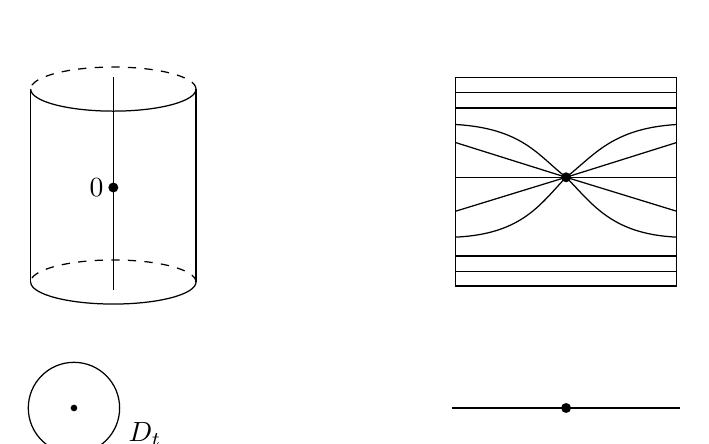
\begin{tikzpicture}[x=1cm,y=1cm,line width=.45pt]
  % Total space and base disc.
  \draw (-4.2,2.6) arc[start angle=180,end angle=360,x radius=1.05,y radius=.28];
  \draw[dashed] (-2.1,2.6) arc[start angle=0,end angle=180,x radius=1.05,y radius=.28];
  \draw (-4.2,2.6)--(-4.2,.15);
  \draw (-2.1,2.6)--(-2.1,.15);
  \draw (-4.2,.15) arc[start angle=180,end angle=360,x radius=1.05,y radius=.28];
  \draw[dashed] (-2.1,.15) arc[start angle=0,end angle=180,x radius=1.05,y radius=.28];
  \draw (-3.15,2.75)--(-3.15,.05);
  \fill (-3.15,1.35) circle (1.8pt);
  \node[left] at (-3.15,1.35) {$0$};
  \draw (-3.65,-1.45) circle (.58);
  \fill (-3.65,-1.45) circle (1.2pt);
  \node[right] at (-3.08,-1.78) {$D_t$};

  % Real slice and its base.
  \draw (1.2,.1) rectangle (4.0,2.75);
  \foreach \yy in {.28,.48,2.36,2.56}{\draw (1.2,\yy)--(4.0,\yy);}
  \draw (1.2,2.15) .. controls (2.05,2.10) and (2.25,1.75) .. (2.60,1.48)
                    .. controls (2.95,1.75) and (3.18,2.10) .. (4.0,2.15);
  \draw (1.2,.72) .. controls (2.05,.76) and (2.28,1.15) .. (2.60,1.48)
                   .. controls (2.93,1.15) and (3.17,.76) .. (4.0,.72);
  \draw (1.2,1.92)--(2.60,1.48)--(4.0,1.92);
  \draw (1.2,1.05)--(2.60,1.48)--(4.0,1.05);
  \draw (1.2,1.48)--(4.0,1.48);
  \fill (2.60,1.48) circle (1.8pt);
  \draw (1.15,-1.45)--(4.05,-1.45);
  \fill (2.60,-1.45) circle (1.8pt);
\end{tikzpicture}
\end{center}

设 $B^+\subset B_{t_0,d_1}$ 是满足
\[
|f(x)|^2\leq\tau(\delta(x)).
\]
的点 $x$ 所构成的集合。设 $\varphi_n$ 为从 $[0,t_0]$ 到 $(0,d_1]$ 的一列 $C^\infty$ 函数，使对某个趋于 $0$ 的序列 $t_0>r_1>r_2>\cdots$，

\begin{enumerate}[label=(\alph*)]
\item 对 $|t|^2\geq r_i$，$\varphi_i$ 是 $\tau$ 的反函数；
\item 对 $|t|^2<r_i$ 及 $j>i$，$\varphi_j(t)<\varphi_i(t)$。
\end{enumerate}

\begin{center}
\begin{tikzpicture}[x=1cm,y=1cm,>=Latex,line width=.5pt]
  \draw[->] (0,0)--(4.5,0) node[right] {$t$};
  \draw[->] (0,0)--(0,3.4) node[above] {$d$};
  \draw (0,3.0)--(3.05,3.0)--(3.05,0);
  \node[left] at (0,3.0) {$d_1$};
  \node[below] at (3.05,0) {$t_0$};
  \draw (0,0) .. controls (.35,1.05) and (1.35,2.15) .. (3.05,2.45);
  \node[right] at (3.05,2.45) {$t=\tau(d)$};
  \draw (0,1.45) .. controls (.45,1.42) and (.80,1.40) .. (1.18,1.68)
        .. controls (1.45,1.88) and (1.68,2.00) .. (1.92,2.10);
  \node at (.55,1.72) {$\varphi_0$};
  \draw (0,.58) .. controls (.23,.56) and (.35,.65) .. (.50,.90)
        .. controls (.67,1.18) and (.84,1.40) .. (1.18,1.68);
\end{tikzpicture}
\end{center}

空间 $B^+-\{0\}$ 是 $D_t$ 上由
\[
\delta(x)\geq\varphi_i(|f(x)|^2).
\]
所定义的丛 $B_i^+$ 的并。利用 $\delta$ 在 $B^+-\{0\}\to D_t$ 的各纤维上无临界点这一事实，标准论证表明：存在与到 $D_t$ 的投影相容的微分同胚 $\alpha_i:B_i^+\to B_{i+1}^+$，在 $B_i^+$ 的子空间
\[
\delta(x)=\varphi_i(|f(x)|^2),
\qquad |f(x)|^2\leq r_i,
\]
的一个小邻域之外等于恒等映射。复合各 $\alpha_i$ 并取极限，得到微分同胚
\[
\alpha:B_0^+-\{x\mid f(x)=0,\ \delta(x)=\varphi_0(0)\}
\xrightarrow{\ \sim\ }B^+-\{0\}.
\]
通过 $\alpha$ 搬运 $D_t$ 上丛 $B_0^+$ 的一个平凡化，得到 $B^+-\{0\}$ 上的可积联络 $\nabla'$。于是可以：

\begin{enumerate}[label=(\alph*)]
\item 将此联络在 $f^{-1}(S_{|y|})\cap B^+$ 上的限制延拓为 $f^{-1}(S_{|y|})/S_{|y|}$ 上的联络；此延拓给出 $T_1$；
\item 将 $\nabla'$ 在 $B^+-\{0\}$ 上给出的 $D_t$ 上径向向量场的提升，延拓至 $B_{t_0,d_1}$。
\end{enumerate}

于是，存在 $B_{t_0,d_1}$ 上唯一的可积联络 $\nabla$，延拓 $\nabla'$、(a) 和 (b)；并存在从 $B_{t_0,d_1}-\{0\}$ 到 $W-\{0\}$ 的唯一水平微分同胚，它在 $f^{-1}(y)$ 上为恒等。这就是所求的微分同胚。


\subsubsection*{3.1.6. 推广。}
前面的讨论可推广到如下情形：$f:X\to D$ 为一个态射，使 $0\in X$ 是\underline{在} $X_0$ 中的孤立非光滑点。缩小 $X$ 和 $D$ 后，$f$ 的非光滑点集在 $D$ 上有限。消灭圈流形 $V$ 具有有限个临界点构成的集合 $\Sigma$；$V-\Sigma$ 是带边界的可微流形（边界紧，但流形不紧）。单值变换 $T$ 在边界上为恒等，并保持 $\Sigma$。最后，命题 3.1.5 仍成立：保持纤维的同胚 $\Psi$ 在临界点集之外是微分同胚，且将临界点集映至 $W$ 中来自 $\Sigma$ 的部分。

\subsubsection*{3.1.7.}
命题 3.1.5 允许使用 1.4 的计算。得到：

\begin{enumerate}[label=(\Alph*)]
\item 消灭圈群 $(R^i\Phi(\Lambda))_0$ 是消灭圈流形 $V$ 以 $\Lambda$ 为系数的约化上同调群。
\item 群 $H^i_{\{0\}}(X_0,R\Psi(\Lambda))$ 是 $V^\circ$ 以 $\Lambda$ 为系数的具有固有支集的上同调群。
\item 变差
\[
  \operatorname{Var}:\widetilde H^i(V,\Lambda)
  \longrightarrow H_c^i(V^\circ,\Lambda)
  =H^i(V\bmod\partial V,\Lambda)
  \]
是由 $V$ 的自同构 $T$ 定义的经典变差，此自同构在 $\partial V$ 上为恒等。
\end{enumerate}

\subsubsection*{3.1.8.}
断言 (A)、(B) 和 (C) 实际上比命题 3.1.5 更初等。下面给出直接的证明与构造，从而无须验证 (A) 和 (B) 中的同构不依赖于 3.1.5 构造过程中的选择。

设 $d\leq r$ 及 $t\leq\tau(d)$，并设 $B$ 是开盒形区域
\[
B=\{x\mid\delta(x)<d\ \text{且}\ |f(x)|^2<t\}.
\]
设 $\widetilde D^*$ 是 $D^*$ 的万有覆盖，考虑将 (1.2.7.2) 限制到 $D_t$ 所得的图
\begin{equation}\tag{3.1.8.1}
\begin{tikzcd}[column sep=large,row sep=large]
\{0\} \arrow[r,hook,"\bar\imath"] \arrow[d,equal]
  & \widetilde D_t \arrow[d,"p"]
  & \widetilde D_t^* \arrow[l,hook',"\bar\jmath"'] \arrow[d,"p'"] \\
\{0\} \arrow[r,hook,"i"]
  & D_t
  & D_t^* \arrow[l,hook',"j"']
\end{tikzcd}
\end{equation}
设
\begin{equation}\tag{3.1.8.2}
\begin{tikzcd}[column sep=large,row sep=large]
B_0 \arrow[r,hook,"\bar\imath"] \arrow[d,equal]
  & \overline B \arrow[d,"p"]
  & \overline B^* \arrow[l,hook',"\bar\jmath"'] \arrow[d,"p'"] \\
B_0 \arrow[r,hook,"i"]
  & B
  & B^* \arrow[l,hook',"j"']
\end{tikzcd}
\end{equation}
是 $f:B\to D$ 在 (3.1.8.1) 上的逆像。仍用 $f$ 表示从 (3.1.8.2) 到 (3.1.8.1) 的投影。

\medskip
\noindent\textup{(A)}
按定义，$R^i\Psi_\eta(\Lambda)_0$ 是当 $U$ 遍历 $X$ 中 $0$ 的各邻域时，上同调群
\[
H^i(U\times_D\widetilde D^*,\Lambda).
\]
的正极限。令 $U$ 遍历由上述盒形区域 $B$ 构成的 $0$ 的基本邻域系。纤维积 $U\times_D\widetilde D^*=\overline B^*$ 是可缩空间 $\widetilde D_t^*$ 上以 $V^\circ$ 为纤维的丛。因此群 $H^i(\overline B^*,\Lambda)$ 的正向系统为常值，取值
\[
H^i(V^\circ,\Lambda)=H^i(V,\Lambda).
\]
所得同构
\begin{equation}\tag{3.1.8.3}
R^i\Psi_\eta(\Lambda)_0\simeq H^i(V,\Lambda)
\end{equation}
可进一步写成如下复合同构（参见下文 (B)）：
\begin{equation}\tag{3.1.8.4}
\begin{tikzcd}[column sep=small,row sep=large,cells={nodes={font=\small}}]
R\Psi_\eta(\Lambda)_0
  & R\Gamma(B_0,R\Psi_\eta(\Lambda)) \arrow[l,"\sim"']
  & (Rf_*R\bar\jmath_*\Lambda)_0 \arrow[l,"\sim"']
  & R\Gamma(\widetilde D_t,Rf_*R\bar\jmath_*\Lambda)
      \arrow[l,"\sim"'] \arrow[d,equal] \\
{}
  & R\Gamma(V,\Lambda) \arrow[r,"\sim"]
  & R\Gamma(V^\circ,\Lambda)
  & R\Gamma(\overline B^*,\Lambda) \arrow[l,"\sim"']
\end{tikzcd}
\end{equation}
复形 $R\Phi(\Lambda)_0$ 由区别三角
\[
\Lambda\longrightarrow(R\Psi_\eta\Lambda)_0
\longrightarrow R\Phi(\Lambda)_0\longrightarrow{}.
\]
定义。因此，群 $R^i\Phi(\Lambda)_0$ 是 $V$ 的约化上同调群。

\medskip
\noindent\textup{(B)}
设 $\mathfrak F$ 是 $\overline B^*$ 的那些在 $\overline B$ 中的闭包在 $\widetilde D$ 上固有的闭子集构成的族。下图中的箭头都是同构：
\begin{equation}\tag{3.1.8.5}
\begin{tikzcd}[column sep=small,row sep=large,cells={nodes={font=\small}}]
R\Gamma_{\{0\}}(R\Psi_\eta(\Lambda))
  \arrow[r,"\sim","\text{\textcircled{1}}"']
  & R\Gamma_c(B_0,R\Psi_\eta(\Lambda))
  & (Rf_!R\bar\jmath_*\Lambda)_0
      \arrow[l,"\sim"',"\text{\textcircled{2}}"] \\
R\Gamma_c(V^\circ,\Lambda)
  & R\Gamma_{\mathfrak F}(\overline B^*,\Lambda)
      \arrow[l,"\sim"',"\text{\textcircled{5}}"]
      \arrow[r,equal,"\text{\textcircled{4}}"']
  & R\Gamma(\widetilde D_t,Rf_!R\bar\jmath_*\Lambda)
      \arrow[u,"\text{\textcircled{3}}","\wr"']
\end{tikzcd}
\end{equation}
事实上，\textcircled{1} 是同构，因为 $B_0$ 是锥体（3.1.2）且 $R^i\Psi_\eta(\Lambda)$ 在 $0$ 外为常值；\textcircled{2} 由固有基变换定理；\textcircled{3} 因为 $Rf_!R\bar\jmath_*\Lambda$ 在 $0$ 外为常值；\textcircled{4} 是复合函子的谱序列的导出范畴形式；\textcircled{5} 因为 $\widetilde D^*$ 可缩。

同构 (3.1.8.5) 给出所求的同构
\begin{equation}\tag{3.1.8.6}
R^i\Gamma_{\{0\}}(R\Psi_\eta(\Lambda))
\simeq H_c^i(V^\circ,\Lambda).
\end{equation}
将在 3.1.10 中验证 (C)。


\subsubsection*{3.1.9.}
参见 [3]。设 $X$ 是拓扑空间，$i:Y\hookrightarrow X$ 是闭子集，$T$ 是 $X$ 的自同构，在 $Y$ 上诱导恒等映射，并设 $\Lambda$ 是交换群。为定义变差 $\operatorname{Var}$，选取 $X$ 上 $\Lambda$ 的一个 $T$-等变消解 $\Lambda_X^*$，以及 $Y$ 上常值层 $\Lambda$ 的一个消解 $\Lambda_Y^*$，约定 $T$ 在其上平凡作用；再选取一个等变态射
\[
\varphi:\Lambda_X^*\longrightarrow i_*\Lambda_Y^*
\]
消解显然的态射 $\varphi_0:\Lambda_X\to i_*\Lambda_Y$。假设层 $\Lambda_X^i$ 与 $\Lambda_Y^i$ 对所考虑的函子均无上同调。取整体截面得
\[
\Gamma(\varphi):\Gamma(\Lambda_X^*)
\longrightarrow\Gamma(\Lambda_Y^*).
\]
为简单起见，假设每个 $\Gamma(\varphi)^i$ 均满；否则，可通过向 $\Gamma(\Lambda_X^*)$ 添加 $\Gamma(\Lambda_Y^*)$ 的锥使其为满。令
\[
R\Gamma(X\bmod Y,\Lambda)=\operatorname{Ker}(\Gamma(\varphi)).
\]
在合理的假设下，若 $\mathfrak F$ 是 $X$ 中与 $Y$ 不交的闭子集构成的族，则有拟同构
\[
\Gamma_{\mathfrak F}(X-Y,\Lambda_X^*)
\xrightarrow{\ \sim\ }R\Gamma(X\bmod Y,\Lambda).
\]
$\Gamma(\Lambda_X^*)$ 的自同态 $T-1$（其中 $T$ 通过搬运结构作用）在 $\Lambda$（常值部分）上为零，并经 $\operatorname{Ker}(\Gamma(\varphi))$ 分解。因此，在导出范畴中且在相同假设下，它给出变差态射
\[
\operatorname{Var}:R\widetilde\Gamma(X,\Lambda)
\longrightarrow R\Gamma_{\mathfrak F}(X-Y,\Lambda).
\]
无这些假设时，则得到
\[
\operatorname{Var}:R\widetilde\Gamma(X,\Lambda)
\longrightarrow R\Gamma(X\bmod Y,\Lambda).
\]

当 $T$ 在 $Y$ 的一个邻域上为恒等，并在该邻域内于 $\Lambda_X^*$ 上平凡作用时，此描述可简化。此时 $\Gamma(\Lambda_X^*)$ 的自同态 $T-1$ 经 $\Gamma_{\mathfrak F}(\Lambda_X^*)$ 分解，并给出变差。

\subsubsection*{命题 3.1.10.}
在 3.1.8(A),(B) 的同构下，变差
\[
(R\Phi_\eta(\Lambda))_0
\longrightarrow R\Gamma_{\{0\}}(R\Psi_\eta(\Lambda))
\]
等于 3.1.9 中由 $V$ 的自同构 $T$ 所定义的变差，此自同构在 $\partial V$ 上为恒等。

建议读者画一张小图来理解，而不必阅读证明。设 ${}_fB$ 是 3.1.2 的闭盒形区域，${}_fC\subset{}_fB$ 是沿其边界的领圈；于是通过将 $\partial_fB\times\{1\}$ 恒等映至 $\partial_fB$ 的一个同构，${}_fC\simeq\partial_fB\times[0,1]$ 成为 $D_t$ 上的丛。设
\[
{}_f\alpha:{}_fC\xrightarrow{\ \sim\ }
(\partial V\times[0,1])\times D_t
\]
为 $D_t$ 上丛 ${}_fC$ 的平凡化，其在 $y\in D_t$ 处的纤维诱导恒等映射
\[
\partial V=\partial(f^{-1}(y))
\xrightarrow{\ \sim\ }\partial V\times\{1\}.
\]
令 $C={}_fC\cap B$，并设
\[
\alpha:C\xrightarrow{\ \sim\ }
(\partial V\times[0,1))\times D_t
\]
由 ${}_f\alpha$ 诱导。保留 (3.1.8.2) 的记号。

设 $R$ 是 $\overline B$ 上由以下规则定义的等价关系：$xRy$，当且仅当 $x=y$，或者 $p(x),p(y)\in C$ 且 $\alpha(p(x))$、$\alpha(p(y))$ 在 $\partial V\times[0,1)$ 中有相同的像。令
\[
{}_1\overline B=\overline B/R,
\qquad
{}_1\overline B^*=\overline B^*/R,
\qquad
{}_1\overline C^*=p^{-1}(C)/R.
\]
有交换图
\[
\begin{tikzcd}[column sep=large,row sep=large]
B_0 \arrow[r,hook,"\bar\imath"] \arrow[d,equal]
  & \overline B \arrow[d,"q"]
  & \overline B^* \arrow[l,hook',"\bar\jmath"'] \arrow[d,"q'"] \\
B_0 \arrow[r,hook,"\bar\imath"]
  & {}_1\overline B
  & {}_1\overline B^* \arrow[l,hook',"{}_1\bar\jmath"']
\end{tikzcd}
\]
设 $\Lambda^*$ 是 $\overline B^*$ 上由无上同调层构成的 $\Lambda$ 的一个 $\pi_1(D^*)$-等变消解。按定义，变差由复形态射
\[
\Lambda[0]\longrightarrow
\bar\imath^*\bar\jmath_*(\Lambda^*).
\]
计算。由于 $\Lambda\xrightarrow{\sim}Rq_*\Lambda$ 且 $\Lambda\xrightarrow{\sim}Rq'_*\Lambda$，也可使用 $\Lambda$ 在 ${}_1\overline B^*$ 上的一个等变消解及态射
\[
\Lambda[0]\longrightarrow
\bar\imath^*{}_1\bar\jmath_*(\Lambda).
\]
来计算。在 (A) 和 (B) 下，变差由此等同于复合态射
\begin{equation}\tag{3.1.10.1}
\begin{tikzcd}[column sep=small,row sep=large,cells={nodes={font=\small}}]
R\Gamma(V,\Lambda) \arrow[r,"\sim"]
  & R\Gamma(V^\circ,\Lambda)
  & R\Gamma({}_1\overline B^*,\Lambda)
      \arrow[l,"\sim"',"\text{\textcircled{1}}"]
      \arrow[d,"\operatorname{Var}"] \\
{}
  & R\Gamma_c(V^\circ,\Lambda)
  & R\Gamma({}_1\overline B^*\bmod{}_1\overline C^*,\Lambda)
      \arrow[l,"\sim"',"\text{\textcircled{2}}"]
\end{tikzcd}
\end{equation}
其中 \textcircled{1} 与 \textcircled{2} 由 $V^\circ$ 到 ${}_1\overline B^*$ 的包含诱导，且 $\operatorname{Var}$ 是 3.1.9 对 ${}_1\overline B^*$ 及 $\pi_1(D^*)$ 的正生成元的作用所定义的变差。此群通过 1.1.5 中描述的作用来作用于 ${}_1\overline B^*$，并平凡地作用于 ${}_1\overline C^*$。

在 $B^*/D^*$ 上选择与 $C$ 的平凡化相容的联络 $\nabla$。此联络平凡化 $\overline B^*$，取商后定义映射 $u:{}_1\overline B^*\to V$。对如 3.1.3 中定义的 $T$，图
\[
\begin{tikzcd}[column sep=large,row sep=large]
{}_1\overline B^* \arrow[r,"u"] \arrow[d,"T"']
  & V \arrow[d,"T"] \\
{}_1\overline B^* \arrow[r,"u"]
  & V
\end{tikzcd}
\]
交换。映射 $u$ 诱导上同调同构，故命题 3.1.10 由 (3.1.10.1) 及变差的函子性得证。

命题 3.1.10 是为后面的一个显式计算提供依据；该计算中同此处一样，$T$ 在 $\partial V$ 的一个邻域上为恒等。我们将取一个由流 $C$ 表示的上同调类 $c$，并使用如下事实：$\operatorname{Var}(c)$ 由在 $V^\circ$ 中具有紧支集的流 $TC-C$ 表示。


\subsubsection*{3.1.11.}
实际中，常将 $T$ 的计算分为两步。

\begin{enumerate}[label=(\alph*)]
\item 固定满足 $t\leq\tau(d)$ 的 $t$ 和 $d$，选择 $y\in D_t^*$，并在 $f^{-1}(S_{|y|})\cap B_{t,d}$ 上选择一个联络 $\nabla$。此联络定义
\[
  V_0=f^{-1}(y)\cap B_{t,d}
  \]
到自身的微分同胚 $T_0$，但它未必在边界上为恒等。
\item 选择 $D_t$ 上 $\partial B_{t,d}$ 的一个平凡化。积分 $\nabla$ 给出从 $\partial V$ 到
\[
  f^{-1}(e^{2\pi i\theta}y)\cap\partial B_{t,d},
  \]
的微分同胚 $\varphi(\theta)$，目标通过平凡化与 $\partial V$ 等同。对 $0\leq\theta\leq1$，$\varphi(\theta)$ 是 $\operatorname{Diff}(\partial V)$ 中从恒等映射连至 $\partial T_0$ 的道路。
\end{enumerate}

所得有序对 $(T_0,\varphi)$ 依赖于所作的任意选择。由于这些选择构成的空间可缩，它在同伦意义下不依赖于这些选择。对 3.1.3 中考虑的变换 $T$，$(T,\text{常值道路})$ 是这里所考虑的一对。

\subsubsection*{3.1.12.}
映射
\[
\operatorname{Diff}(V)\longrightarrow\operatorname{Diff}(\partial V)
\]
是纤维化。因此，赋值 $T\mapsto(T,\text{常值道路})$ 诱导以下两者间的双射：

\begin{enumerate}[label=\alph*)]
\item 满足 $\partial T=\operatorname{id}$ 的微分同胚 $T:V\to V$，相差同痕视为相同；以及
\item 有序对 $(T_0,\varphi)$，其中 $T_0:V\xrightarrow{\sim}V$，$\varphi$ 是从 $\operatorname{id}$ 到 $\partial T_0$ 的道路的同伦类，相差同痕视为相同。
\end{enumerate}

因此，由 3.1.11(a),(b) 算出的一对 $(T_0,\varphi)$ 确定 $T$。具体地，由 $(T_0,\varphi)$ 计算 $T$ 如下。

\medskip
\noindent\textup{($\alpha$)} 选择领圈嵌入
\[
  [0,1]\times\partial V\xhookrightarrow{\ \alpha\ }V,
  \qquad \alpha(1,x)=x,
  \]
及一个代表
$\varphi:[0,1]\to\operatorname{Diff}(\partial V)$
使将其在负参数处定义为 $\operatorname{id}$ 所得的延拓为 $C^\infty$ 的。在领圈上令
\[
  \beta(x)=\operatorname{pr}_1\alpha^{-1}(x).
  \]
于是 $\beta$ 无临界点，取值于 $[0,1]$，且在 $\partial V$ 上等于 $1$。

\medskip
\noindent\textup{($\beta$)} 在领圈之外取 $T=T_0$，在领圈上令
\[
  T(x)=T_0\bigl(\varphi(\beta(x))^{-1}(x)\bigr).
  \]

\subsubsection*{3.1.13.}
下面是 3.1.11(b) 的一种变体，用以计算道路 $\varphi$ 的同伦类。在每条射线 $\arg(z)=\theta$ 上，选择丛 $\partial B_{t,d}$ 的一个随 $\theta$ 连续变化的平凡化。使用过 $y$ 的射线上的平凡化，将
\[
(\partial V)_0=f^{-1}(0)\cap\partial B_{t,d}
\]
等同于 $\partial V$。设
\[
\Psi_\theta:V\longrightarrow
f^{-1}(e^{i\theta}y)\cap B_{t,d}
\]
由积分 $\nabla$ 得到。将 $\partial\Psi_\theta$ 沿射线搬运，得到 $(\partial V)_0$、从而 $\partial V$ 到自身的微分同胚。这就是 $\varphi(\theta)$。
\subsection*{3.2. Picard--Lefschetz 公式（超越情形）}

\subsubsection*{3.2.1.}
对映射
\[
f=\sum_{i=1}^{n+1}z_i^2:\mathbb C^{n+1}\longrightarrow\mathbb C.
\]
我们将把 3.1 的结果具体写出。对 $\delta$ 取函数 $\sum |z_i|^2$，并取由
\[
\left|\sum z_i^2\right|\leq a^2,
\qquad
\sum |z_i|^2\leq b^2,
\]
定义的盒形区域 $B=B_{a,b}$，其中 $0<a<b$。使用闭盒形区域而非 3.1.2 中的盒形区域，只是为了简化记号。

\subsubsection*{3.2.2.}
消灭圈流形 $V$ 的方程为
\begin{equation}\tag{3.2.2.1}
\begin{array}{rcl}
\displaystyle\sum z_i^2&=&a^2,\\
\displaystyle\sum |z_i|^2&\leq&b^2.
\end{array}
\end{equation}
将 $z=(z_i)$ 用其实部与虚部写成 $z=x+iy$。前述方程化为
\begin{equation}\tag{3.2.2.2}
\begin{array}{rcl}
x^2-y^2&=&a^2,\\
x\mathbin{\cdot}y&=&0
  \qquad\bigl(\text{即 }x\perp y\text{ 位于 }\mathbb R^{n+1}\bigr),\\
x^2+y^2&\leq&b^2.
\end{array}
\end{equation}
\footnote{原印本在 (3.2.2.2) 中写作 $\mathbb R^n$，但 $z$ 有 $n+1$ 个坐标。英文文本将这一明显的维数笔误改为 $\mathbb R^{n+1}$。}
在 $V$ 上引入新坐标系
\[
X=\frac{x}{|x|},
\qquad
Y=y\left(\frac{b^2-a^2}{2}\right)^{-1/2}.
\]
于是 $x=X(a^2+y^2)^{1/2}$，且 (3.2.2.2) 化为
\begin{equation}\tag{3.2.2.3}
\begin{array}{rcl}
X^2&=&1,\\
X\mathbin{\cdot}Y&=&0,\\
Y^2&\leq&1.
\end{array}
\end{equation}
这将 $V$ 等同于球面 $S^n$ 的切球丛。

\subsubsection*{3.2.3.}
映射
\[
\theta\longmapsto \exp(2\pi i\theta)a^2
\]
将 $\mathbb R$ 等同于 $\mathbb C$ 中以 $0$ 为中心、半径为 $a^2$ 的圆周 $S_{a^2}$ 的万有覆盖。丛 $B$ 到 $\mathbb R$ 的拉回同构于 $\mathbb R\times V$。
我们通过从 $V$ 到 $B$ 在 $\exp(2\pi i\theta)a^2$ 上的纤维的同构
\[
v\longmapsto \exp(\pi i\theta)v
\]
将其平凡化。设 $T_0$ 是此平凡化按 3.1.11 给出的映射。在坐标 (3.2.2.3) 中，
\[
T_0(X,Y)=(-X,-Y).
\]
\begin{editorialnote}
原文在 3.2.1、3.2.2 采用 $f=a^2$，但 3.2.3、3.2.4 的基点及圆盘半径写作 $a$。这里统一保留前面的 $f=a^2$ 约定，将后两节的基点、圆周及圆盘半径写为 $a^2$；乘以 $e^{\pi i\theta}$ 的平凡化公式不变。
\end{editorialnote}

\subsubsection*{3.2.4.}
作为“丛” $B$ 的边界的、半径为 $a^2$ 的圆盘 $D_{a^2}$ 上的丛，其方程为
\[
\sum |z_i|^2=b^2,
\qquad
f(z)\in D_{a^2},
\]
到圆盘的投影为 $f$。下面描述此丛在每条射线
\[
e^{2\pi i\theta}\mathbb R^+\cap D_{a^2}.
\]
上的逆像的一个平凡化。

在射线 $\mathbb R^+\cap D_{a^2}$ 上，取到 $(\mathbb R^+\cap D_{a^2})\times\partial V$ 的同构，它在 $\partial V$ 上的坐标 (3.2.2.3) 中由
\[
z=x+iy\longmapsto(f(z),X,Y)
  =\left(f(z),\frac{x}{|x|},\frac{y}{|y|}\right).
\]
给出。在 $(e^{2\pi i\theta}\mathbb R^+)\cap D_{a^2}$ 上，使用此平凡化在乘以 $e^{\pi i\theta}$ 下的像。应用 3.1.13，并在 $\partial V$ 上使用满足
\begin{equation}\tag{3.2.4.1}
X^2=Y^2=1,
\qquad
X\mathbin{\cdot}Y=0.
\end{equation}
的坐标 $(X,Y)$。若 $\varphi(\theta)$ 将 $(X,Y)$ 映至 $(X_\theta,Y_\theta)$，则算得
\begin{equation}\tag{3.2.4.2}
X_\theta+iY_\theta
=e^{\pi i\theta}(X+iY)
\qquad(0\leq\theta\leq1).
\end{equation}

\subsubsection*{3.2.5.}
总之，消灭圈流形 $V$ 是 $S^n$ 的切球丛。单值变换由 $(T_0,\varphi)$ 表示，其中 $T_0$ 是对径映射的微分，而 $\varphi$ 是从 $\operatorname{Id}$ 到 $\partial T_0$ 的如下道路：在 $\varphi(\theta)$ 下，将每个单位切向量沿它所确定的测地线平行移动距离 $-\pi\theta$（负号意为“沿向量所指的反方向”）\EditorialFootnote{原文此处写 $+\pi\theta$。但 (3.2.4.2) 给出 $X_\theta=\cos(\pi\theta)X-\sin(\pi\theta)Y$，故基点的初速度为 $-\pi Y$，沿单位切向量的反方向运动。负号也与紧接着给出的 $-\pi(1-\varphi(|u|))$ 的单值变换公式相符。}。在 $\theta=1$ 时到达对径向量。

由 3.1.12，得到 $T$ 的如下描述。\EditorialFootnote{原文这里引用 3.1.13。由有序对 $(T_0,\varphi)$ 加入领圈修正以构造 $T$ 的公式实际在 3.1.12；3.1.13 给出的是边界道路同伦类的计算变体。}设 $\varphi:[0,1]\to[0,1]$ 是 $C^\infty$ 映射，在 $0$ 附近为 $0$，在 $1$ 附近为 $1$。映射 $T$ 将 $u$ 沿 $u$ 所确定的测地线移动距离
\[
-\pi\bigl(1-\varphi(|u|)\bigr).
\]
在 $|u|=1$ 附近它为恒等映射；在 $|u|=0$ 附近它为对径映射。
\subsubsection*{3.2.7.}
设 $W$ 是 $d$ 维可微流形，设
\[
p:T(W)\longrightarrow W
\]
为其切丛，视为流形。若 $(x_1,\ldots,x_d)$ 为 $W$ 上的局部坐标系，则
\[
(x_1,\ldots,x_d,dx_1,\ldots,dx_d)
\]
为 $T(W)$ 上的局部坐标系。设 $\varepsilon'$ 为此坐标系定义的 $T(W)$ 的定向。它不依赖于 $x_i$ 的选择，因而在整体上定义。

假设 $W$ 可定向。子流形 $W\subset T(W)$（零截面）配上一个定向（分别为其法丛的一个定向），定义 $H_d(T(W))$（分别为 $H_c^d(T(W))$）中的元素 $w$。$W\subset T(W)$ 的自相交为 Euler--Poincaré 示性数：
\[
\int w\wedge w=\chi(W)
\]
这里使用定向 $\varepsilon'$。

\footnote{原印本此句混用了三个维数符号：将维数记为 $x$，将坐标下标写至 $n$，并将上同调类放在 $d$ 次。英文文本在一般陈述中统一使用 $d$；下文的特殊情形使用 $d=n$。}

对消灭圈流形 $V$，其复结构定义定向 $\varepsilon$。它与 $S^n$ 的切丛的定向 $\varepsilon'$ 的关系为
\[
\varepsilon=(-1)^{\frac{n(n-1)}2}\varepsilon'.
\]

\subsubsection*{3.2.8.}
\underline{消灭圈} $\delta$ 在相差符号的意义下良定义。对 $n\ne0$，它是由子流形 $S^n\subset V^\circ$ 定义的 $H_c^n(V^\circ)$ 中的元素。对 $n=0$，空间 $V$ 由两点组成，$\delta$ 是它们之差。使用 $V$ 的复定向，3.2.7 给出
\begin{equation}\tag{3.2.8.1}
(\delta,\delta)
=(-1)^{\frac{n(n-1)}2}\bigl(1+(-1)^n\bigr).
\end{equation}

\subsubsection*{3.2.9.}
令
\[
\widetilde H_c^i(V^\circ)
=\operatorname{Ker}\!\left(
H_c^i(V^\circ)\xrightarrow{\ \operatorname{Tr}\ }\mathbb Z
\right);
\]
当 $i\ne2n$ 时这就是 $H_c^i(V^\circ)$。则
\[
\begin{aligned}
\widetilde H_c^i(V^\circ)&=0 &&\text{当 }i\ne n,\\
\widetilde H_c^n(V^\circ)&=\mathbb Z,
  &&\text{由下列元素生成：}\delta.
\end{aligned}
\]
对偶地，
\[
\begin{aligned}
\widetilde H^i(V)&=0 &&\text{当 }i\ne n,\\
\widetilde H^n(V)&\xrightarrow[\sim]{\ (\,\cdot\,,\delta)\ }\mathbb Z.
\end{aligned}
\]
对 $n\ne0$，$\delta\in H_c^n(V^\circ)$ 在 $H^n(V)$ 中的像在 $n$ 为奇数时为零，在 $n$ 为偶数时可被二整除（且不能再整除）。
\subsubsection*{3.2.10.}
来计算变差
\[
\operatorname{Var}:\widetilde H^n(V)
\longrightarrow H_c^n(V^\circ).
\]
先使用定向 $\varepsilon'$ 并假设 $n\ne0$。设 $\alpha$ 是 $S^n$ 的切丛的一个定向，并设 $\delta\in H_c^n(V^\circ)$ 由 $S^n\subset V^\circ$ 及其法丛的定向 $\alpha$ 定义。满足 $(\delta',\delta)=1$ 的上闭链 $\delta'\in H^n(V)$ 由 $V^\circ$ 到 $S^n$ 的纤维化的一个纤维表示。此纤维的法丛为以 $S^n$ 上一点处的切空间为值的常值丛，并赋予定向 $\alpha$。

此断言不依赖于定义映射
\[
(\text{子流形 + 其法丛的定向})
\longrightarrow\text{上同调}.
\]
时所选的符号约定。事实上，改变约定会将 $\delta$ 换为 $-\delta$，同时将 $\delta'$ 换为 $-\delta'$。当
\[
\operatorname{Tr}:H_c^{2n}(V,\mathbb R)\longrightarrow\mathbb R
\]
定义如下时，断言成立：
\begin{description}[leftmargin=2.8em,labelsep=.5em]
\item[\textup{($\alpha$)}] 由于 $\Omega_V^*$ 是 $\underline{\mathbb R}$ 的软消解，$\Gamma_c(\Omega_V^*)$ 表示 $R\Gamma_c(V,\mathbb R)$，从而有同构
\[
  H^i\bigl(\Gamma_c(V,\Omega_V^*)\bigr)
  \simeq H_c^i(V,\mathbb R)
  \]
（不使用迭代上边缘）；
\item[\textup{($\beta$)}] $\operatorname{Tr}$ 为积分。
\end{description}

类 $T(\delta')$ 在 $\partial V$ 的一个邻域上与 $\delta'$ 一致，因此
\(
\operatorname{Var}(\delta')=T(\delta')-\delta'
\)
在 $V^\circ$ 中有紧支集。有
\[
T(\delta')-\delta'\sim-\delta,
\qquad\text{因而}
\]
\[
\operatorname{Var}(\delta')
=-(\delta',\delta)\,\delta.
\]

以下是 $n=1$ 的图示。画出 $S^1$ 的切丛，使沿 $S^1$ 所选逆时针定向的向量朝外。

\begin{center}
\begin{tikzpicture}[>=Latex,line width=.45pt,scale=.92]
  \begin{scope}[shift={(-2.8,0)}]
    \draw (0,0) circle (2.15);
    \draw (0,0) circle (1.20);
    \draw (0,0) circle (.43);
    \draw (0,.43)--(0,2.15);
    \draw[->] (-.02,1.88)--(-.48,1.88);
    \draw[->] (-.02,1.13)--(-.48,1.13);
    \node[right] at (.10,1.10) {$\delta'$};
    \draw[->] (-.85,.85)--(-1.16,1.16);
    \draw[->] (-.85,-.85)--(-1.17,-1.17);
    \node[above left] at (-1.02,-.98) {$\delta$};
    \draw[->] (.85,-.85)--(1.17,-1.17);
    \draw[->] (1.43,1.12)--(1.43,1.72)
      node[right] {$2$};
    \draw[->] (1.43,1.12)--(.83,1.12)
      node[below] {$1$};
    \node at (1.03,1.63) {$\varepsilon$};
    \node[below=5pt] at (0,-2.15)
      {$\delta,\ \delta'\ \text{且}\ \varepsilon$};
  \end{scope}
  \begin{scope}[shift={(2.8,0)}]
    \draw (0,0) circle (2.15);
    \draw (0,0) circle (.43);
    \draw (0,.43)--(0,2.15);
    \draw
      (0,2.15)
      .. controls (.02,1.68) and (1.18,1.42) .. (1.28,.30)
      .. controls (1.40,-.72) and (.62,-1.35) .. (-.12,-1.31)
      .. controls (-1.05,-1.27) and (-1.42,-.42) .. (-1.10,.48)
      .. controls (-.83,1.10) and (-.34,1.25) .. (0,1.02);
    \draw[->] (1.08,.78)--(.74,.48);
    \node[below=5pt] at (0,-2.15)
      {$\operatorname{Var}(\delta')$};
  \end{scope}
\end{tikzpicture}
\end{center}

因此，对定向 $\varepsilon$，有
\[
\operatorname{Var}(x)
=-\frac{\varepsilon}{\varepsilon'}(x,\delta)\,\delta.
\]

\subsubsection*{定理 3.2.11.}
\underline{群 $\widetilde H_c^n(V^\circ)$ 同构于 $\mathbb Z$，由消灭圈 $\delta$ 生成。群 $\widetilde H^n(V)$ 也同构于 $\mathbb Z$，且与前一群对偶。其余各群 $\widetilde H_c^i(V^\circ)$ 与 $\widetilde H^i(V)$ 均为零。}

\medskip
\noindent\underline{变差由下式给出}
\[
\operatorname{Var}(x)
=-(-1)^{\frac{n(n-1)}2}(x,\delta)\,\delta,
\qquad\underline{\text{且}}
\]
\[
(\delta,\delta)
=(-1)^{\frac{n(n-1)}2}\bigl(1+(-1)^n\bigr).
\]
根据 $n$ 模 $4$ 的同余类，有下表：
\[
\begin{array}{lcccc}
n\bmod4&0&1&2&3\\[2pt]
(\delta,\delta)&2&0&-2&0\\[2pt]
\operatorname{Var}(x)=\pm(x,\delta)\delta&-&-&+&+\\[2pt]
T(\delta)=(-1)^{n+1}\delta&-\delta&\delta&-\delta&\delta
\end{array}
\]
作为核验，确实有
\[
T(\delta)=\delta+\operatorname{Var}(\delta).
\]
\section*{4. de Rham 上同调}

\subsubsection*{4.1.}
设 $D$ 是复解析圆盘，$0\in D$，令 $D^*=D-\{0\}$，并设 $\widetilde D^*$ 是 $D^*$ 的一个万有覆盖。设 $X$ 是解析空间，$f:X\longrightarrow D$ 是态射，并考虑 (1.2.7.1) 的图：
\begin{equation}\tag{4.1.1}
\begin{tikzcd}[column sep=large,row sep=large]
X_0 \arrow[r,hook,"\bar i"] \arrow[d,equal]
  & \bar X \arrow[d,"p"']
  & \bar X^* \arrow[l,hook',"\bar j"'] \arrow[d,"p'"'] \\
X_0 \arrow[r,hook,"i"]
  & X
  & X^* \arrow[l,hook',"j"']
\end{tikzcd}
\end{equation}
假设 $X^*=X-X_0$ 非奇异（即光滑）。因此其覆盖 $\bar X^*$ 也光滑。用 $\Omega_{\bar X^*}^*$ 表示 $\bar X^*$ 上全纯微分形式层的 de Rham 复形。它是常值层 $\mathbb C$ 的消解（全纯 Poincaré 引理），因而给出 $D^+(\bar X,\mathbb C)$ 中的态射
\begin{equation}\tag{4.1.2}
\bar j_*\Omega_{\bar X^*}^*
\longrightarrow R\bar j_*\mathbb C
\end{equation}

\subsubsection*{命题 4.2.}
\underline{态射 (4.1.2) 是同构。}

显然，(4.1.2) 在 $\bar X^*\subset\bar X$ 的每一点处都是拟同构。\footnote{原印本的证明写作 (4.1.1)，那是前面的图而非所讨论的态射；英文恢复了显然应有的引用 (4.1.2)。}
因此，只需证明每个点 $x\in X_0$ 在 $\bar X$ 中都有一个基本邻域系 $U$，使
\[
H^q\bigl(\bar j^{-1}(U),\Omega^p\bigr)=0
\qquad\text{当 }q>0.
\]
当 $V$ 遍历 $X$ 中 $x$ 的一个基本邻域系时，各集合 $p^{-1}(V)$ 构成 $\bar X$ 中 $x$ 的一个基本邻域系。特别地，可取 $p^{-1}(V)$，其中 $V$ 是 $X$ 中 $x$ 的一个 Stein 邻域。若 $V$ 为 Stein，则 $V-X_0$ 仍为 Stein（因为 $X_0\cap V$ 在 $V$ 中由一个方程定义），其覆盖
\[
p'^{-1}(V-X_0)=\bar j^{-1}p^{-1}(V).
\]
也为 Stein。因此，对 $\bar X^*$ 上的每个凝聚层 $\mathcal F$，
\[
H^q\bigl(\bar j^{-1}p^{-1}(V),\mathcal F\bigr)=0
\qquad\text{当 }q>0,
\]
命题得证。

\subsubsection*{推论 4.3.}
\underline{同构 (4.1.2) 诱导同构}
\begin{equation}\tag{4.3.1}
\bar i^*\bar j_*\Omega_{\bar X^*}^*
\xrightarrow{\ \sim\ }R\Psi_\eta(\mathbb C).
\end{equation}

\subsubsection*{变体 4.4.}
\underline{设 $V$ 是 $X^*$ 上的有限维复向量空间局部常值层（复局部系统）。Poincaré 引理的拟同构}
\[
V\longrightarrow\Omega_{X^*}^*(V)
\]
\underline{诱导拟同构}
\begin{equation}\tag{4.4.1}
\bar i^*\bar j_*\Omega_{\bar X^*}^*(p'^*V)
\xrightarrow{\ \sim\ }R\Psi_\eta(V).
\end{equation}

我们将证明：将 $\bar i^*\bar j_*\Omega_{\bar X^*}^*$ 换为由增长条件和单值条件定义的一个子复形后，(4.3.1) 仍成立。
\subsubsection*{4.5.}
设 $f:X^*\longrightarrow D^*$ 是 $D^*$ 上的拓扑空间，$F$ 是 $X^*$ 上的 $f^\circ\mathcal O_{D^*}$-模层，$\bar F$ 是它在
\[
\bar X^*=X^*\times_{D^*}\widetilde D^*.
\]
上的逆像。

设 $z:D\hookrightarrow\mathbb C$ 是全纯嵌入，$z(0)=0$。下文总允许缩小 $D$；对足够小的圆盘，$z$ 的存在性是显然的。在 $\widetilde D^*$ 上选择函数 $\log z$ 使 $\exp(\log z)=z$，并令
\[
z^\alpha=\exp(\alpha\log z)
\qquad(\alpha\in\mathbb C).
\]

群 $\pi_1(D^*)$ 通过搬运结构作用于 $H^0(\bar X^*,\bar F)$。若一个元素 $f\in H^0(\bar X^*,\bar F)$ 在 $\pi_1(D^*)$ 作用下的各变换张成一个有限维复向量空间 $V(f)$，则称其为\underline{有限决定型}（finite determination）。设 $T$ 是 $\pi_1(D^*)$ 的正生成元。截面 $f$ 为有限决定型，当且仅当存在非零多项式 $P\in\mathbb C[X]$ 使 $P(T)(f)=0$。此时具有这一性质的最低次数多项式，既是 $T$ 在 $V(f)$ 上作用的最小多项式，也是其特征多项式。

若存在 $A$ 使
\[
(T-1)^A f=0.
\]
则称 $f$ 为\underline{幺幂有限决定型}。在这些截面构成的空间上定义
\[
N=\frac{\log T}{2\pi i}
\]
其作用由有限和
\[
N(f)=-\frac1{2\pi i}
\sum_{n>0}\frac{(1-T)^n}{n}\,f.
\]
给出。
若 $f$（分别为 $g$）是 $H^0(D^*,\mathcal O)$（分别为 $H^0(\bar X^*,\bar F)$）中的幺幂有限决定型截面，则
\[
N(fg)=N(f)g+fN(g),
\]
因为自同构的对数是导子。

若存在 $A$ 和 $B>0$ 使
\[
(T^B-1)^A f=0.
\]
则称 $f$ 为\underline{拟幺幂有限决定型}。

\subsubsection*{例 4.6.}
对 $X=D^*$ 和 $F=\mathcal O$，有
\[
\bigl(T-\exp(2\pi i\alpha)\bigr)^{k+1}
  \bigl(z^\alpha(\log z)^k\bigr)=0,
\]
\[
N(\log z)=1,
\]
以及
\[
N\left(\frac{(\log z)^k}{k!}\right)
=\frac{(\log z)^{k-1}}{(k-1)!},
\qquad
(0\text{ 当 }k=0).
\]

\subsubsection*{命题 4.7.}
\underline{截面 $f\in H^0(\bar X^*,\bar F)$ 为有限决定型，当且仅当它可写成}
\begin{equation}\tag{4.7.1}
f=\sum_{\alpha,k}f_{\alpha,k}\,
z^\alpha\frac{(\log z)^k}{k!},
\end{equation}
\underline{其中 $0\leq\operatorname{Re}(\alpha)<1$，$k\in\mathbb N$，且各 $f_{\alpha,k}\in H^0(X^*,F)$ 几乎全为零。对有限决定型的 $f$，分解 (4.7.1) 唯一。}

由 4.6，每个形如 (4.7.1) 的截面都为有限决定型。反之，设 $f$ 为有限决定型，且 $P(T)(f)=0$。写成
\[
P(X)=\prod_{\beta\in\mathbb C}(X-\beta)^{n'(\beta)}
=\prod_{0\leq\operatorname{Re}(\alpha)<1}
 \bigl(X-\exp(2\pi i\alpha)\bigr)^{n(\alpha)},
\]
其中 $n(\alpha)=n'(\exp(2\pi i\alpha))$ 几乎全为零。将 $\mathbb C[X]$-模 $V(f)$ 分解为其同型分量，得到唯一的分解
\[
f=\sum_\alpha f'_\alpha
\]
使
\[
\bigl(T-\exp(2\pi i\alpha)\bigr)^{n(\alpha)}f'_\alpha=0.
\]

选择多项式 $Q_\alpha\in\mathbb C[X]$，使其模 $\bigl(X-\exp(2\pi i\alpha)\bigr)^{n(\alpha)}$ 同余于 $1$，且对每个 $\alpha'\ne\alpha$，模 $\bigl(X-\exp(2\pi i\alpha')\bigr)^{n(\alpha')}$ 同余于 $0$。于是 $f'_\alpha=Q_\alpha(T)(f)$。令
\begin{equation}\tag{4.7.2}
f_\alpha=z^{-\alpha}f'_\alpha
=z^{-\alpha}Q_\alpha(T)(f).
\end{equation}
由于
\[
T(z^{-\alpha}f'_\alpha)
=\exp(-2\pi i\alpha)z^{-\alpha}T(f'_\alpha),
\]
有
\[
(T-1)^{n(\alpha)}f_\alpha=0.
\]

若
\[
f_\alpha=\sum_k f_{\alpha,k}\frac{(\log z)^k}{k!},
\qquad f_{\alpha,k}\in H^0(X^*,F),
\]
则由 4.6 及恒等式 $\sum_j(-1)^j\binom{k}{j}=\delta_{0,k}$ 得
\begin{equation}\tag{4.7.3}
f_{\alpha,k}
=\sum_{j\geq0}(-1)^j\frac{(\log z)^j}{j!}
  N^{j+k}f_\alpha,
\end{equation}
这证明唯一性。

反之，若 $f_\alpha$ 是幺幂有限决定型截面，则 (4.7.3) 定义的各 $f_{\alpha,k}$ 在 $k$ 足够大时为零（因为 $k$ 足够大时 $N^k f_\alpha=0$），且在 $T$ 下不变；因而它们可等同于 $X^*$ 上 $F$ 的截面。等价地，须证明 $Nf_{\alpha,k}=0$。将恒等式
\[
\begin{aligned}
N\sum_{j\geq0}(-1)^j\frac{(\log z)^j}{j!}N^j
&=\sum_{j>0}(-1)^j\frac{(\log z)^{j-1}}{(j-1)!}N^j\\
&\quad+\sum_{j\geq0}(-1)^j\frac{(\log z)^j}{j!}N^{j+1}=0.
\end{aligned}
\]
应用于 $N^k f_\alpha$。最后，
\[
\sum_{k\geq0}f_{\alpha,k}\frac{(\log z)^k}{k!}
=\sum_{j,k\geq0}(-1)^j
 \frac{(\log z)^{j+k}}{j!k!}N^{j+k}f_\alpha
\]
\[
=\sum_{n\geq0}
 \left(\sum_j(-1)^j\binom nj\right)
 \frac{(\log z)^n}{n!}N^n f_\alpha
=f_\alpha,
\]
这就证明了 4.7。

\subsubsection*{注 4.8.1.}
4.7 中的条件 $\operatorname{Re}(\alpha)\in[0,1)$ 可换为 $\alpha\in C$，其中 $C$ 是 $\mathbb C\longrightarrow\mathbb C/\mathbb Z$ 的任意基本域。

\subsubsection*{注 4.8.2.}
设 $f$ 为有限决定型，其分解为 (4.7.1)。对 $0\leq\operatorname{Re}(\alpha)<1$ 及满足某个 $f_{\alpha,k}\ne0$ 的 $\alpha$，令
\[
m(\alpha)=1+\sup\{k\mid f_{\alpha,k}\ne0\}.
\]
若所有 $f_{\alpha,k}$ 均为零，则令 $m(\alpha)=0$。$T$ 在 $V(f)$ 上作用的特征多项式为
\[
\operatorname{Pc}(T,V(f))
=\prod_\alpha\bigl(X-\exp(2\pi i\alpha)\bigr)^{m(\alpha)}.
\]
特别地，$f$ 为拟幺幂有限决定型，当且仅当 (4.7.1) 中的各 $\alpha$ 均可取在 $\mathbb Q$ 中。
\subsubsection*{4.9.}
回到 4.1 的较强假设，设 $F$ 是 $X$ 上的凝聚层，其在 $X^*$ 上的限制局部自由。

\subsubsection*{命题 4.10.}
\underline{设 $f$ 是 $F$ 在 $\bar X^*$ 上的逆像 $\bar F$ 的一个有限决定型截面。则 $f$ 沿 $X_0$ 适度增长，当且仅当分解 (4.7.1) 中的各 $f_{\alpha,k}$ 沿 $X_0$ 亚纯。}

“适度增长”的定义见 [1], 2.10。由 (4.7.1)、(4.7.2) 和 (4.7.3) 可清楚看出，$f$ 适度增长当且仅当各 $f_{\alpha,k}$ 适度增长。对 $X^*$ 上 $F$ 的截面，已知沿 $X_0$ 适度增长等价于沿 $X_0$ 亚纯。

对 $X=D$ 及 $F=\mathcal O$，4.10 有如下初等推论。

\subsubsection*{推论 4.11.}
\underline{设 $K$ 为 $D$ 上亚纯函数在 $0$ 处的芽构成的域，并设 $K^m$（分别为 $K^{mu}$ 和 $K^{mqu}$）为 $\widetilde D^*$ 上在 $0$ 处适度增长且为有限决定型（分别为幺幂有限决定型和拟幺幂有限决定型）的全纯函数在 $0$ 处的芽构成的 $K$-代数。则以下分别是它们在 $K$ 上的基：}
\[
\begin{array}{lll}
K^m:&z^\alpha(\log z)^k,
  &0\leq\operatorname{Re}(\alpha)<1,\ k\in\mathbb N,\\[2pt]
K^{mu}:&(\log z)^k,&k\in\mathbb N,\\[2pt]
K^{mqu}:&z^\alpha(\log z)^k,
  &\alpha\in\mathbb Q,\ 0\leq\alpha<1,\ k\in\mathbb N.
\end{array}
\]

在 4.9 的假设下，用 $\Psi_\eta^m(F)$（分别用 $\Psi_\eta^{mu}(F)$ 与 $\Psi_\eta^{mqu}(F)$）表示 $\bar i^*\bar j_*\bar F$ 的如下子层：它由 $\bar F$ 在 $X_0$ 的各点附近、沿 $X_0$ 适度增长且为有限决定型（分别为幺幂有限决定型和拟幺幂有限决定型）的截面构成。设
\[
F^m\subset j_*j^*F
\]
为 $X$ 上由 $j_*j^*F$ 中沿 $X_0$ 亚纯的截面所成的层。命题 4.10 有下述不依赖于 $z$ 和 $\log z$ 的任意选择的推论。

\subsubsection*{推论 4.12.}
\underline{自然态射}
\[
\textup{(i)}\qquad
K^m\otimes_K i^*F^m\longrightarrow\Psi_\eta^m(F),
\]
\[
\textup{(ii)}\qquad
K^{mu}\otimes_K i^*F^m\longrightarrow\Psi_\eta^{mu}(F),
\]
\[
\textup{(iii)}\qquad
K^{mqu}\otimes_K i^*F^m\longrightarrow\Psi_\eta^{mqu}(F)
\]
\underline{都是同构。}

本节的主要结果如下。

\subsubsection*{定理 4.13.}
\underline{由 (4.3.1) 诱导的自然态射}
\begin{equation}\tag{4.13.1}
\Psi_\eta^{mqu}(\Omega_X^*)
\longrightarrow R\Psi_\eta(\mathbb C),
\end{equation}
\underline{是 $D^+(X_0,\mathbb C)$ 中的同构。}

实际上，我们将证明更一般的结果 4.15 和 4.17。它们的陈述需要一些预备知识；只关心 4.13 的读者可以略过。

\subsubsection*{4.14.}
设 $V$ 是 $X^*$ 上的有限维复向量空间局部常值层（局部系统）。设
\[
\mathcal V=V\otimes_{\mathbb C}\mathcal O
\]
为相应的局部自由 $\mathcal O$-模，设 $\nabla$ 是 $\mathcal V$ 上使 $V$ 的局部截面水平的可积联络。已知 $\mathcal V$ 可延拓为 $X$ 上的凝聚层 $\widetilde{\mathcal V}$，使 $\nabla$ 相对于此延拓沿 $X_0$ \underline{正则}。还已知任意两个这样的延拓亚纯等价（[1], II, 5.7）。因此，层 $\Psi_\eta^m(\widetilde{\mathcal V})$ 及其变体 $\Psi^{mu}$ 与 $\Psi^{mqu}$ 不依赖于所选的延拓；将其记为 $\Psi_\eta^m(\mathcal V)$。同样定义
\[
\Psi_\eta^m\bigl(\Omega_{X^*}^p(V)\bigr)
=\Psi_\eta^m(\Omega_X^p\otimes\mathcal V),
\]
及其变体 $\Psi^{mu}$ 与 $\Psi^{mqu}$。

\subsubsection*{命题 4.15.}
\underline{由 (4.4.1) 诱导的自然态射}
\begin{equation}\tag{4.15.1}
\Psi_\eta^m\bigl(\Omega_{X^*}^*(V)\bigr)
\longrightarrow R\Psi_\eta(V),
\end{equation}
\underline{是 $D^+(X_0,\mathbb C)$ 中的同构。}

\subsubsection*{4.16.}
若对每个从标准圆盘 $D_0$ 到 $X$、满足 $u^{-1}(X_0)=\{0\}$ 的态射 $u$，$D_0^*$ 上局部系统 $u^*V$ 的单值变换均为幺幂（分别为拟幺幂），则称 4.14 中的局部系统 $V$ 沿 $X_0$ \underline{幺幂}（分别为\underline{拟幺幂}）。

\subsubsection*{命题 4.17.}
\underline{若 $V$ 拟幺幂，则由 (4.4.1) 诱导的自然态射}
\begin{equation}\tag{4.17.1}
\Psi_\eta^{mqu}\bigl(\Omega_{X^*}^*(V)\bigr)
\longrightarrow R\Psi_\eta(V),
\end{equation}
\underline{是 $D^+(X_0,\mathbb C)$ 中的同构。}

定理 4.13 是 4.17 中 $V=\underline{\mathbb C}$ 的特殊情形。
\subsubsection*{4.18.}
先处理 $X$ 光滑且 $(X_0)_{\mathrm{red}}$ 是 $X$ 中的正规交叉除子的情形。由于各定理是局部的，可假设 $f$ 是从 $X=D^e$ 到 $D$ 的映射
\[
f(\underline z)=\prod_{i=1}^d z_i^{n_i},
\qquad 0<d\leq e,\quad n_i>0,
\]
这里 $D$ 表示标准圆盘 $D=\{z\in\mathbb C\mid |z|<1\}$。只需证明 (4.15.1)（分别为 (4.17.1)）在 $0\in D^e$ 处的纤维是拟同构。

设 $U$ 是 $D^e$ 中 $0$ 的形如 $|z_i|<a$ 的邻域，其中 $0<a\leq1$。在 (4.1.1) 中取 $U$ 的逆像，定义 $U_0$、$\bar U$、$U^*$ 和 $\bar U^*$。$U^*$ 或 $\bar U^*$ 的上同调不依赖于 $a$，因此
\[
H^*(\bar U^*,V)\xrightarrow{\ \sim\ }
  \bigl(R^*\Psi_\eta(V)\bigr)_0.
\]
$X^*=(D^*)^d\times D^{e-d}$ 的基本群 $\mathbb Z^d$（也是 $U^*$ 的基本群）为交换群。因此 $V$ 具有一个有限滤过，其相继商为秩一局部系统。通过逐步化简，可假设 $V$ 秩为一。

对 4.14 中的 $\widetilde{\mathcal V}$，用 $j_*^m\Omega_{X^*}^*(V)$ 表示 $j_*\Omega_{X^*}^*(V)$ 的子复形，其 $p$ 次项为 $(\Omega_X^p\otimes\widetilde{\mathcal V})^m$。由 [1], II 6.4.1 和 6.8，拟同构 $V\xrightarrow{\ \approx\ }\Omega_{X^*}^*(V)$（全纯 Poincaré 引理）诱导的自然映射
\begin{equation}\tag{4.18.1}
j_*^m\Omega_{X^*}^*(V)\longrightarrow Rj_*V,
\end{equation}
是拟同构。因此
\begin{equation}\tag{4.18.2}
H^*\bigl((j_*^m\Omega_{X^*}^*(V))_0\bigr)
 \xrightarrow{\ \sim\ }(R^*j_*V)_0
 \xleftarrow{\ \sim\ }H^*(U^*,V).
\end{equation}
\footnote{原印本 (4.18.2) 右端为 $H^*(U,V)$，但 $V$ 定义在 $U^*$ 上；英文恢复了显然应有的 $U^*$。}
这是证明的 4.18 部分唯一使用的解析结果。

\subsubsection*{引理 4.18.3.}
\underline{对秩一的 $V$，有}

\noindent\textup{(i)}\qquad
\uline{若 $V$ 非平凡：}\quad $H^*(U^*,V)=0$，

\medskip
\noindent\textup{(ii)}\qquad
\uline{若 $V=\underline{\mathbb C}$：}\quad
$H^*(U^*,V)=\bigwedge\nolimits^*\mathbb C^d$。

事实上，$U^*$ 具有环面的同伦型。

设 $\eta$ 是 $H^1(D^*,\mathbb Z)$ 的生成元，也表示其在 $H^1(U^*,\mathbb Z)$ 中的逆像。

\subsubsection*{引理 4.18.4.}
\underline{对秩一的 $V$，自然映射}
\[
H^*(U^*,V)
 \xrightarrow[(4.18.1)]{\ \sim\ }
H^*\bigl((j_*^m\Omega_{X^*}^*(V))_0\bigr)
 \longrightarrow
H^*\bigl(\Psi_\eta^{mu}(\Omega_{X^*}^*(V))_0\bigr)
\]
\underline{将 $H^*(\Psi_\eta^{mu}(\Omega_{X^*}^*(V))_0)$ 等同于 $H^*(U^*,V)/\eta H^*(U^*,V)$。}
\footnote{原印本左端为 $H^*(U^*,\mathbb C)$，但假设与结论涉及的都是一般的秩一系统 $V$；英文恢复为 $V$。}

使用 4.12(ii) 以及恒等式 $d\log f=\sum_i n_i\,dz_i/z_i$。复形 $\Psi_\eta^{mu}(\Omega_{X^*}^*(V))_0$ 等同于由双复形 $K$（使用直和）关联的单复形 $\mathrm{s}K$，其各项为
\[
K^{-p,n+p}=\frac{(\log f)^p}{p!}\cdot
  (j_*^m\Omega_{X^*}^n(V))_0.
\]
此复形位于一个不良象限 $(p\leq0,q\geq0,p+q\geq0)$ 中。不过，$\mathrm{s}K$ 是子复形 $\mathrm{s}\,\sigma_{p\geq p_0}(K)$ 的归纳极限，其各项为
\[
(\mathrm{s}\,\sigma_{p\geq p_0}K)^n
=\bigoplus_{\substack{p+q=n\\p\geq p_0}}K^{pq},
\]
这已足以使下面的论证成立。

按第一次数滤过的谱序列为
\[
E_1^{-p,n+p}=H^n(U^*,V)\qquad(p\geq0),
\]
其中
\[
d_1=2\pi i\,\eta\wedge:
H^n(U^*,V)\longrightarrow H^{n+1}(U^*,V).
\]
若 $V$ 非平凡，则由 4.18.3 得 $E_1=0$，而 4.18.4 归结为 $0=0$。假设 $V=\underline{\mathbb C}$。此时复形 $(E_1,d_1)$ 为可能截断的 Koszul 复形，由 Koszul 复形的无上同调性，得到
\[
E_2^{pq}=0\qquad\text{当 }p\ne0,
\]
及
\[
E_2^{0n}=H^n(U^*,V)/\eta H^{n-1}(U^*,V),
\]
这就证明了 4.18.4。

对 $\beta\in\mathbb C^*$，用 $V_\beta$ 表示 $D^*$ 上的秩一局部系统，其在 $\widetilde D^*$ 上的逆像已平凡化，而其单值为 $\beta$。其在 $U^*$ 上的逆像也使用相同记号。在 $\bar U^*$ 上，$V\otimes V_\beta$ 的逆像典范同构于 $V$ 的逆像。

\subsubsection*{引理 4.18.5.}
\underline{对秩一的 $V$，映射}
\[
\bigoplus_{\beta\in\mathbb C^*}
H^*(U^*,V\otimes V_\beta)/
 \eta H^*(U^*,V\otimes V_\beta)
\longrightarrow H^*(\bar U^*,V)
\]
\underline{是双射。}

设 $k$ 为各 $n_i$ 的最大公因数。空间 $\bar U^*$ 有 $k$ 个连通分支，以 $k$ 次单位根为指标。在以 $\xi$ 为指标的分支 $\bar U_\xi^*$ 上，$\widetilde D^*$ 上函数 $z^{1/k}$ 的逆像等于 $U^*$ 上函数
\[
\xi\prod_{i=1}^d z_i^{n_i/k}
\]
的逆像。分支 $\bar U_\xi^*$ 具有环面的同伦型，且序列
\[
0\longrightarrow\pi_1(\bar U_\xi^*)
 \longrightarrow\pi_1(U^*)\longrightarrow\pi_1(D^*)
\]
正合。用 $\varphi:\mathbb Z^d\to\mathbb Z$ 表示映射 $\pi_1(U^*)\to\pi_1(D^*)$。若 $\ker(\varphi)$ 在 $V$ 上作用非平凡，则 4.18.5 两端都为零。\footnote{原印本此处引用 4.18.4；所讨论的两端属于 4.18.5。}
否则，将 $V$ 换为适当的 $V\otimes V_\beta$ 后，可假设 $V$ 平凡，即 $V=\mathbb C$。此时在复上同调中有
\[
H^0(\bar U^*)\otimes
 H^*(U^*)/\eta H^*(U^*)
 \xrightarrow{\ \sim\ }H^*(\bar U^*).
\]
只需注意到：当 $\beta^k=1$ 时 $V_\beta$ 在 $U^*$ 上平凡，以及
\[
\bigoplus_{\beta^k=1}H^0(U^*,V_\beta)
=\bigoplus_{\beta^k=1}\mathbb C
 \xrightarrow{\ \sim\ }H^0(\bar U^*,\mathbb C),
\]
且当 $\beta^k\ne1$ 时 $H^*(U^*,V_\beta)=0$，便得结论。

\subsubsection*{注 4.18.6.}
若 $V$ 拟幺幂，4.18.5 中对 $\mathbb C^*$ 的求和可换为对单位根的求和；证明相同。

应用 4.12 得到交换图
\begin{center}
\begin{tikzcd}[
  column sep=2.2em,
  row sep=large,
  cells={nodes={font=\scriptsize}}
]
H^*\Psi_\eta^m(\Omega_{X^*}^*(V))_0
  \arrow[d]
& \displaystyle\bigoplus_\beta
  H^*\Psi_\eta^{mu}(\Omega_{X^*}^*(V\otimes V_\beta))
  \arrow[l,"\sim"',"4.12"]
& \displaystyle\bigoplus_\beta
  H^*(U^*,V\otimes V_\beta)/
    \eta H^*(U^*,V\otimes V_\beta)
  \arrow[l,"\sim"',"4.18.4"]
  \arrow[d,"\wr"',"4.18.5"]
\\
H^*R\Psi(V)_0
& {}
& H^*(\bar U^*,V)\arrow[ll,"\sim"']
\end{tikzcd}
\end{center}
由此得到 4.15。将 $\Psi^m$ 换为 $\Psi^{mqu}$，将对 $\beta$ 的求和换为对单位根的求和，并将 4.18.5 换为 4.18.6，即得命题 4.17。

\subsubsection*{4.19.}
从特殊情形 4.18 推出 4.15 和 4.17。设 $u:Y\longrightarrow X$ 是 $(X,X_0)$ 的一个消解，即诱导同构 $Y^*\xrightarrow{\ \sim\ }X^*$ 的固有态射，使 $Y$ 光滑且 $(Y_0)_{\mathrm{red}}$ 为 $Y$ 中的正规交叉除子。若 $V$ 沿 $X_0$ 拟幺幂，则其逆像 $u^*V$ 沿 $Y_0$ 拟幺幂。

对 $X$ 上的每个凝聚层 $F$，用 $F^m$ 或 $j_*^m j^*F$ 表示 $j_*j^*F$ 中由亚纯截面构成的子层。若 $f$ 为 $X_0$ 的一个方程，则 $j_*^m j^*F$ 是系统
\begin{equation}\tag{4.19.1}
F\xrightarrow{f}F\xrightarrow{f}F\longrightarrow\cdots.
\end{equation}
的归纳极限。以下引理的证明见 [2]。

\subsubsection*{引理 4.19.2.}
\underline{对 $X$ 上的每个凝聚层 $F$，有}
\[
F^m\xrightarrow{\ \sim\ }u_*(u^*F)^m
\]
\underline{且对 $i>0$ 有 $R^iu_*(u^*F)^m=0$。}

由 Grauert 定理，各 $R^iu_*u^*F$ 为凝聚层。$F\longrightarrow u_*u^*F$ 的核与余核，以及 $i>0$ 时的 $R^iu_*u^*F$，在 $X_0$ 外均为零，因而局部地被 $f$ 的某个幂零化。由于 $u$ 固有，$R^iu_*$ 与滤过归纳极限交换，特别地与归纳极限 (4.19.1) 交换，由此得到 (4.19.2)。

由 4.19.2 与 4.12 推出：在上述假设下，仍用 $u$ 表示 $u$ 诱导的映射 $Y_0\to X_0$，则有下述结论。

\subsubsection*{引理 4.19.3.}
\underline{态射}
\[
\Psi_\eta^m(F)\longrightarrow
u_*\Psi_\eta^m(u^*F)\longrightarrow
Ru_*\Psi_\eta^m(u^*F)
\]
\underline{都是同构。}

第二个箭头为同构意味着
\[
R^iu_*\Psi_\eta^m(u^*F)=0\qquad(i>0).
\]
这由 4.12 及 $i>0$ 时 $R^iu_*(i^*u^*F^m)=0$ 推出；后者又由 $i>0$ 时 $R^iu_*(u^*F^m)=0$ 和 $u$ 的固有基变换定理推出。

为证明 4.15，只需考虑交换图
\begin{center}
\begin{tikzcd}[
  column sep=large,
  row sep=large,
  cells={nodes={font=\small}}
]
\Psi^m(\Omega_{X^*}^*(V))
  \arrow[d]
  \arrow[r,equal,"(4.19.3)"']
& u_*\Psi^m(\Omega_{Y^*}^*(u^*V))
  \arrow[r,"\sim","(4.19.3)"']
& Ru_*\Psi^m(\Omega_{Y^*}^*(u^*V))
  \arrow[d,"\wr"',"(4.18)"]
\\
R\Psi(V)
  \arrow[rr,"(1.3.1;\ \mathrm{XIII}\ 2.1.7.1)"]
& {}
& Ru_*R\Psi(u^*V)
\end{tikzcd}
\end{center}
4.17 的证明相同，只需将所有 $\Psi^m$ 换为 $\Psi^{mqu}$。

\subsubsection*{注 4.20.}
定理 4.13 给出了单值定理在复形层次上的一个体现。

\subsection*{参考文献}

\begin{enumerate}[label={[\arabic*]},leftmargin=3em]
\item P. Deligne, \emph{Equations diff\'erentielles \`a points
  singuliers r\'eguliers}, Lecture Notes in Mathematics 163,
  Springer-Verlag.
\item A. Grothendieck, \emph{On the De Rham cohomology of algebraic
  varieties}, Publ. Math. IHES \underline{29}, 95--103 (1966).
\item K. Lamotke, \emph{Isolated critical points and monodromy}.
\end{enumerate}

\clearpage
\renewcommand{\CurrentExpose}{第 XV 讲}
\phantomsection\addcontentsline{toc}{section}{第 XV 讲}
\begin{center}\underline{第 XV 讲}\end{center}
\clearpage
\begin{center}
{\large SGA 7 --- 第 XV 讲}\par
\vspace{2em}
{\Large\underline{Picard--Lefschetz 公式}}\par
\vspace{1.5em}
{\large P. Deligne}
\end{center}

\medskip
\noindent\textbf{原书目录}
\begin{center}
\begin{tabular}{@{}llr@{}}
\S1. & 普通二次奇点(正规形) & 2\\
1.1 & 回顾 & 2\\
1.2 & 普通二次奇点 & 4\\
1.3 & 二次奇点的模 & 10\\
\S2. & 标准普通二次情形的消灭圈计算 & 13\\
2.1 & 预备: 锥的上同调 & 13\\
2.2 & 消灭圈 & 17\\
\S3. & Picard--Lefschetz 公式 & 23\\
3.1 & 预备结果 & 23\\
3.2 & 偶相对维数 & 24\\
3.3 & 奇相对维数 & 26\\
3.4 & 汇总 & 31
\end{tabular}
\end{center}

\section*{1. 普通二次奇点(正规形)}

本节重新讨论 VI 6 的结果, 采用“Hensel”观点而非“形式”观点. 我们给出普通二次奇点(ordinary quadratic singularities)及其形变的正规形; 在平展拓扑下局部可以将它们化为这些正规形.

这些结果容易由 VI 6、隐函数定理(Tougeron 的形式)以及 R. Elkik 关于孤立奇点的万有 Hensel 模的定理推出. 在讨论班口头报告时, 后一定理尚未问世; 当时已证明一个仅适用于完全交的较弱定理(这已足够我们使用), 该定理将不予发表.

\subsection*{1.1. 回顾}

\subsubsection*{1.1.1.}
设 $f:X\longrightarrow S$ 为态射, $X$ 局部可由 $S$ 上相对维数为 $n+p$ 的仿射空间 $\mathbb A_S^{n+p}$ 中的 $p$ 个方程描述. Jacobian 理想 $J^n(X/S)$ 已在 VI 5 中定义. 若 $X$ 是由方程 $f_i=0$ $(1\leq i\leq p)$ 定义的 $\mathbb A_S^{n+p}$ 的闭子概形, 则它是由 Jacobian 矩阵 $(\partial f_i/\partial x_j)$ 的 $p\times p$ 子式生成的理想层. 以下定理是众所周知的. 其形式版本的一个特例见 Bourbaki, \emph{Alg\`ebre commutative}, III, \S4, no.~6, 定理 2 的推论 3; $C^\infty$ 版本见 Tougeron, \emph{Id\'eaux de fonctions diff\'erentiables}(学位论文, Rennes, 1967 年 5 月); 此处所考虑的情形见 Artin, \emph{Algebraic approximation of structures over complete local rings}, Publ. Math. IHES \underline{36}(Zariski 专卷), 引理 5.10.

\subsubsection*{定理 1.1.2 (Tougeron--Artin).}
\underline{设 $S$ 为 Hensel 局部环 $A$ 的谱, $f:X\to S$ 为 1.1.1 中的态射, $a$ 和 $I$ 为 $A$ 的两个真理想, $\delta'$ 为 $X$ 上包含于 $J^n(X/S)$ 的理想层. 假设 $I$ 为有限型. 设 $s$ 为 $f$ 在 $S/I$ 上的截面, 即 $s\in X(A/I)$. 以 $s^*\delta'^2$ 表示 $A/I$ 的理想 $s^*\delta'^2$ 在 $A$ 中的逆像理想.}

\underline{若 $(s^*\delta'^2)\,a\supset I$, 则存在 $f$ 的截面 $s_1\in X(A)$, 它模 $(s^*\delta')\,a$ 与 $s$ 同余.}

\subsubsection*{1.1.3.}
设 $S$ 为 Hensel 局部环的谱, 闭点为 $s$. 设 $X'_0$ 为 $k(s)$ 上的有限型概形, 在某一闭点 $x_0$ 之外光滑, 并设 $X_0$ 为 $X'_0$ 在 $x_0$ 处的 Hensel 化. 我们考虑下列类型的系统
\begin{center}
\begin{tikzcd}[column sep=large,row sep=large]
X_0 \arrow[r,hook] \arrow[d]
  & X \arrow[d]
  & {} \\
s \arrow[r,hook]
  & T \arrow[r]
  & S
\end{tikzcd}
\end{center}
其条件如下:
\begin{enumerate}[label=(\alph*),leftmargin=2.6em]
\item $T$ 为 Hensel 局部概形, 且在 $S$ 上本质有限表现(I 0.0.5); 态射 $T\to S$ 为局部态射, 并诱导剩余域的同构;

\item $X$ 为 Hensel 局部概形, 且在 $T$ 上平坦而本质有限表现;

\item $X/T$ 的特殊纤维带有一个到 $X_0$ 的 $k(s)$-同构.
\end{enumerate}
这些系统称为 $X_0$ 的 \underline{Hensel $S$-形变}. 从 $(X,T)$ 到 $(X',T')$ 的一个\underline{态射}是一个 $S$-概形的交换图
\begin{center}
\begin{tikzcd}[column sep=large,row sep=large]
X \arrow[r] \arrow[d] & X' \arrow[d] \\
T \arrow[r] & T'
\end{tikzcd}
\end{center}
它在取特殊纤维后诱导 $X_0$ 的恒等态射. 一个形变 $X/T$ 称为\underline{万有的}(versal, 极小万有的), 如果:
\begin{enumerate}[label=(\alph*),leftmargin=2.6em]
\item 对每个使 $T''\to T'$ 为闭浸入的态射 $X''/T''\longrightarrow X'/T'$, 映射
\[
\operatorname{Hom}(X'/T',X/T)
\longrightarrow\operatorname{Hom}(X''/T'',X/T)
\]
为满射. 特别地, 取 $X''/T''=X_0/s$, 有 $\operatorname{Hom}(X'/T',X/T)\ne\varnothing$;

\item 对 $T'=\operatorname{Spec}(k(s)[\varepsilon]/(\varepsilon^2))$, “逆像”映射
\[
\operatorname{Hom}(T',T)\longrightarrow
\{\text{$X_0$ 在 $T'$ 上的形变的同构类}\}
\]
为双射.
\end{enumerate}

\subsubsection*{定理 1.1.4 (R. Elkik).}
\underline{存在 $X_0$ 的一个万有 Hensel $S$-形变(且在非唯一同构的意义下唯一). 若 $S$ 为 Noether 概形, 则形变 $X/T$ 是这样的形变, 当且仅当 $X$ 在 $T$ 的完备化 $\widehat T$ 上诱导 $X_0$ 的一个万有形式 $S$-形变(极小形式万有形变; VI 1.9 及 VI 4).}

这个精细定理的证明参见 R. Elkik(ENS 讨论班, 1971/72).
\subsection*{1.2. 普通二次奇点}

设 $y$ 为特征 $p$ 的域 $k$ 上有限型概形 $Y$ 的闭点, $n$ 为 $Y$ 在 $y$ 处的维数.

\subsubsection*{定义 1.2.1 (= VI 6.6).}
\begin{enumerate}[label=(\roman*),leftmargin=2.6em]
\item \underline{若 $k$ 代数闭, 则称 $y$ 为 $Y$ 的普通二次点, 如果 $Y$ 在 $y$ 处局部环的完备化 $\widehat{\mathcal O}_{Y,y}$ 同构于 $k[[x_1,\ldots,x_{n+1}]]$ 模一个由单个形式幂级数 $f$ 生成的理想的商, 其中该幂级数可写成}
\begin{equation}\tag{1.2.1.1}
f(\underline X)=Q(\underline X)+\text{阶}>2\text{ 的项},
\end{equation}
\underline{且 $Q(\underline X)$ 为普通二次型.}
\footnote{印本中此公式编号为 (4.2.1), 且在 $Q(\underline X)$ 后多了一个等号; 英译恢复了本节编号, 并将展开式恢复为所断言的 $f=Q+$ 高次项.}

\item \underline{若 $\bar k$ 为 $k$ 的代数闭包, 则称 $y$ 为 $Y$ 的普通二次点, 如果 $\bar Y=Y\otimes_k\bar k$ 中位于 $y$ 上方的各点都是 $\bar Y$ 的普通二次点.}
\end{enumerate}

\subsubsection*{1.2.2.}
在此定义中将“普通二次型”换成“非退化二次型”, 就得到\underline{非退化二次点}的概念(VI 6.0). 点 $y$ 是 $Y$ 的非退化二次点, 当且仅当它为普通二次点, 并且 $p\ne2$ 与“$n$ 为奇数”两者至少成立其一.

\subsubsection*{例 1.2.3.}
设 $Q(\underline X)$ 为 $k$ 上的 $n+1$ 元非退化二次型. 设 $Y_0$ 为 $\mathbb A_k^{n+1}$ 中由方程 $Q=0$ 给出的二次锥. 则原点(记作 $y_0$)为 $Y_0$ 的非退化二次点.

\subsubsection*{例 1.2.4.}
假设 $p=2$ 且 $n=2m$. 设 $a\in k$, 并设 $Q$ 为多项式
\[
Q(\underline X)=(X_0^2-a)
 +\sum_{0<i\leq j\leq2m}a_{ij}x_ix_j.
\]
假设 $2m$ 元二次型 $\sum_{0<i\leq j}a_{ij}x_ix_j$ 非退化, 并以 $y_0$ 表示 $\mathbb A_k^{n+1}$ 中坐标为 $(\sqrt a,0,\ldots,0)$ 的闭点. 则 $y_0$ 为由方程 $Q=0$ 定义的闭子概形 $Y_0\subset\mathbb A_k^{n+1}$ 的普通二次点.

\subsubsection*{例 1.2.5.}
设 $k'$ 为 $k$ 的有限可分扩张, $Y_0$ 为 1.2.3(分别为 1.2.4)所考虑类型的 $k'$-概形. 若将 $Y_0$ 看作 $k$-概形, 则 $y_0$ 为 $Y_0$ 的非退化(分别为普通)二次点. 扩张 $k'/k$ 可等同于 $k(y_0)/k$ 的最大可分子扩张.

\subsubsection*{定理 1.2.6.}
\underline{假设 $y$ 为 $k$-概形 $Y$ 的普通二次点, 设 $k'$ 为 $k(y)/k$ 的最大可分子扩张. 则存在 1.2.3 或 1.2.4 中那样的 $k'$-概形 $Y_0\subset\mathbb A_{k'}^{n+1}$, 以及 $Y$ 在 $y$ 处的 Hensel 化 $Y_{(y)}$ 与 $Y_0$ 在 $y_0$ 处的 Hensel 化 $Y_{0(y_0)}$ 之间的 $k$-同构 $\varphi$.}

首先注意, $y$ 在 $Y$ 中存在一个平展邻域 $Y'$
\begin{center}
\begin{tikzcd}[row sep=large,column sep=large]
{} & Y'\arrow[d]\\
y\arrow[ur,hook]\arrow[r,hook]&Y
\end{tikzcd}
\end{center}
它是一个 $k'$-概形. 实际上, $Y_{(y)}$ 典范地是 $k'$-概形. 将 $(k,Y,y)$ 换为 $(k',Y',y)$ 后, 就归结为 $k=k'$ 的情形, 即 $k(y)/k$ 为纯不可分扩张的情形.
$k(y)$-向量空间 $(\Omega^1_{Y/k})_y$ 的维数为 $n+1$. 将标量从 $k(y)$ 扩张到其代数闭包, 并在 $y$ 处完备化后检验即可; 此时结论显然. 因而 $Y$ 中 $y$ 的一个邻域是某个维数为 $n+1$ 的光滑 $k$-概形 $Z$ 的闭子概形. 此外, 将 $Y$ 和 $Z$ 换成适当的 $y$ 的邻域后, $\mathcal O_Z$ 中定义 $Y$ 的理想为主理想(论证同上), 设其方程为 $f$.

\subsubsection*{引理 1.2.7.}
\underline{假设 $y$ 是 $Y$ 的非退化二次点, 且 $k(y)/k$ 为纯不可分扩张. 则在 $y$ 的一个邻域中, $J^n_{Y/k}$ (1.1.1)由一个元素生成, 支集为 $y$, 在 $k$ 上秩为一. 特别地, $k(y)=k$.}

转到 $k$ 的代数闭包并在 $y$ 处完备化后证明第一个断言即可. 此时直接计算即可得出: 采用 1.2.1 的记号, Nakayama 引理表明 $\partial f/\partial x_i$(从而更有 $f$ 及 $\partial f/\partial x_i$)生成极大理想.

现在对非退化的 $y$ 证明 1.2.6. 可以而且将假设 $k(y)=k$, $Y$ 在光滑概形 $Z$ 中由一个方程 $f$ 定义, 且有将 $y$ 映到 $0$ 的平展态射
\[
x:Z\longrightarrow\mathbb A_k^{n+1}
\]
(一个“局部坐标系 $x_i$”). 于是存在 $n+1$ 元非退化二次型 $Q$, 使在 $y$ 处有
\[
f=Q(x_i)+\text{次数为 }>2.
\]
设 $Y_0$ 如 1.2.3 中那样由 $Q$ 定义.\footnote{印本此处引用 4.3; 刚使用的正规形实际为例 1.2.3.}

\underline{在 $Y$ 上}, 系统 $(x_i)$ 为方程 $Q(x_i)=0$ 的一个“近似解”: 若 $\mathfrak m$ 是定义 $y$ 的理想, 则
\[
Q(x_i)\in\mathfrak m^3\qquad\text{在 }Y.
\]
由于 $Q$ 非退化, $\mathbb A_k^{n+1}$ 上由 $\partial Q/\partial x_i$ 生成的理想就是 $0$ 处的极大理想, 它在 $x=(x_i):Y\to\mathbb A_k^{n+1}$ 下的逆像为 $\mathfrak m$. 由隐函数定理 1.1.2(取 $a=\mathfrak m$ 及 $\delta'=J$), Hensel 化 $Y_{(y)}$ 上存在函数 $x'_i$, 模 $\mathfrak m^2$ 与 $x_i$ 同余, 且满足 $Q(x'_i)=0$. 它们给出所求的 $Y_{(y)}$ 与 $Y_{0(y_0)}$ 之间的同构.

\subsubsection*{引理 1.2.8.}
\underline{假设 $y$ 为退化的普通二次点($p=2$ 且 $n$ 为偶数), 并假设 $k(y)/k$ 为纯不可分扩张. 则在 $y$ 的一个邻域中, $T^1_{Y/k}$ 由一个元素生成, 支集为 $y$, 在 $k$ 上秩为二. 特别地, 或者 $k(y)=k$, 或者对某个 $a\in k$, $a\notin k^2$, $k(y)$ 同构于 $k(\sqrt a)$.}

采用 1.2.7 的方法. 用 1.2.1 的记号, 只需检验
\[
\dim_k\left(
k[[x_1,\ldots,x_{n+1}]]\big/
  (f,\partial f/\partial x_i)
\right)=2.
\]
在适当坐标 $x_0,x_1,\ldots,x_{2m}$ 下, 形式幂级数 $f$ 可写为
\[
f=x_0^2+\sum_{i=1}^m x_ix_{i+m}+R,
\qquad\operatorname{ord}(R)\geq3.
\]
设 $\mathfrak n'$ 为由 $f$ 和 $\partial f/\partial x_i$ 生成的理想, $\mathfrak n$ 为由 $x_0^2$ 及 $i\ne0$ 的 $x_i$ 生成的理想, $\mathfrak q$ 为极大理想. 我们证明 $\mathfrak n=\mathfrak n'$. 显然 $\mathfrak n'\subset\mathfrak n$, 由 Nakayama 引理, 只需检验
\[
\mathfrak n'+\mathfrak n\mathfrak q=\mathfrak n.
\]
模 $\mathfrak n\mathfrak q$, 有 $f\equiv x_0^2$; 模 $\mathfrak n\mathfrak q+(x_0^2)$, 有
\[
\frac{\partial f}{\partial x_i}\equiv x_{i+m},
\qquad
\frac{\partial f}{\partial x_{i+m}}\equiv x_i
\qquad(1\leq i\leq m),
\]
这就证明了断言.

在 1.2.8 的假设下, 若 $k=k(y)$, 则以 $a$ 表示 $k$ 中任意一个平方.

\subsubsection*{引理 1.2.9.}
\underline{设 $V$ 为概形 $S$ 上的向量丛, $T$ 为 $\mathbb A_S(V)$ 中在 $S$ 上局部自由秩为二的闭子概形. 则 $T$ 包含在 $\mathbb A_S(V)$ 中唯一的一条直线内.}

此问题对于 $S$ 上的 fppf 拓扑是局部的, 因此可假设 $T/S$ 有截面. 经过平移, 可假设 $T$ 包含零截面. 设 $\mathfrak n$ 为 $T$ 中定义 $0$ 的理想; 它在 $S$ 上局部自由秩为一. $\mathbb A_S(V)$ 上每个齐次线性形式 $v\in V$ 都定义 $\mathfrak n$ 的一个元素, 从而得到满射 $V\twoheadrightarrow\mathfrak n$. 其核定义所求直线.

\subsubsection*{1.2.10.}
特别地, 若 $A$ 是特征 $2$ 的域 $k$ 上仿射空间 $\mathbb A_k^{n+1}$ 的纯不可分秩二闭子概形, 则存在 $a\in k$, 使在适当的仿射坐标下, $A$ 的方程为
\[
x_0^2-a=0,
\qquad x_i=0\quad(1\leq i\leq n).
\]
只需取在 $A$ 所确定的直线上消失的 $x_i$.

\subsubsection*{1.2.11.}
现在对退化的 $y$($p=2$ 且 $n=2m$)证明 1.2.6. 可以而且将假设 $k(y)=k(\sqrt a)$, $Y$ 在光滑概形 $Z$ 中由一个方程 $f$ 定义, 且在 $y$ 处存在一个局部坐标系
\[
x=(x_i)_{0\leq i\leq2m}:
Z\longrightarrow\mathbb A_k^{2m+1}
\]
将 $y$ 映到闭点 $(\sqrt a,0,\ldots,0)$, 使在 $y$ 的一个邻域中有
\[
J^n_{Y/k}\simeq
\mathcal O_Y/(x_0^2-a,x_1,\ldots,x_{2m}).
\]
将 $f$ 换成适当的倍数后, 有
\[
f=(x_0^2-a)+
 \sum_{1\leq i\leq j\leq2m}a_{ij}x_ix_j+R,
\]
其中
\begin{enumerate}[label=(\alph*),leftmargin=2.6em]
\item $2m$ 元二次型 $\sum a_{ij}x_ix_j$ 非退化;
\item 将标量扩张到 $\bar k$ 后, $R$ 关于 $x_0-\sqrt a$ 和 $x_i$ 的阶至少为 $3$.
\end{enumerate}
设 $Y_0$ 如 1.2.4 中那样由下式定义:
\[
Q=x_0^2-a+\sum a_{ij}x_ix_j.
\]

\underline{在 $Y$ 上}, 系统 $(x_i)$ 仍可视作 $Q(X_i)=0$ 的近似解. 这一次, 由 $\partial Q/\partial X_i$ 生成的理想在 $x$ 下的逆像 $\delta$ 满足 $\mathcal O_Y/\delta\simeq J^n_{Y/k}$; 在 $y$ 处它为
\[
\delta=(x_0^2-a,(x_i)_{1\leq i}).
\]
设 $\mathfrak q$ 为定义 $y$ 的极大理想. 为了像非退化情形那样应用隐函数定理得出结论, 尚须检验
\begin{equation}\tag{1.2.11.1}
Q(x_i)\equiv0\pmod{\delta^2\mathfrak q}
\qquad\underline{\text{在 }Y}.
\end{equation}
设 $\bar{\mathfrak q}$ 为将标量扩张到 $k$ 的代数闭包后定义 $y$ 的理想. 可检验
\[
\delta^2\bar{\mathfrak q}\cap\mathcal O_{Y,y}
=\delta^2\mathfrak q.
\]
因此, 将标量扩张到 $\bar k$ 后验证 (1.2.11.1) 即可; 可假设 $a=0$.\footnote{印本此处引用 (4.11.1); 正在证明的同余式是 (1.2.11.1).}
在 $y$ 处于是有
\[
\delta^2\mathfrak q=
(x_0^5,(x_0^3x_i)_{1\leq i},
 (x_0x_ix_j)_{1\leq i,j},
 (x_ix_jx_k)_{1\leq i,j,k}).
\]
由此 $\delta^2\mathfrak q\supset\mathfrak q^5$, 并且
\[
x_0^2f\equiv x_0^4\pmod{\delta^2\mathfrak q},
\qquad
\delta^2\mathfrak q+(x_0^2f)\supset\mathfrak q^4,
\]
\[
x_0f\equiv x_0^3
 \pmod{\delta^2\mathfrak q+\mathfrak q^4},
\qquad
\delta^2\mathfrak q+(x_0f)\supset\mathfrak q^3.
\]
最后,
\[
Q(x_i)\equiv0\pmod{\delta^2\mathfrak q+(f)}
\qquad\underline{\text{在 }Z},
\]
这就是 (1.2.11.1).

\subsubsection*{注 1.2.12.}
设 $Q$ 为不必齐次的 $n+1$ 元非零二次型, 并假设由方程 $Q$ 定义的闭子概形 $Y\subset\mathbb A_k^{n+1}$ 在某点 $y$ 处有普通二次奇点. 则经过一个非齐次线性换元, 可将 $Y$ 化为 1.2.3 或 1.2.4 的形式. 非退化时 $k(y)=k$, 只须将 $y$ 移到原点. 退化时, 只须使 $T^1_{Y/k}$ 的支集落在直线 $x_i=0$ $(1\leq i\leq2m)$ 上(参见 1.2.9).
\subsection*{1.3. 二次奇点的模}

以下命题由 R. Elkik 的定理 1.1.4 以及留给读者的显式计算推出(这些计算本质上已包含于 VI 6).

\subsubsection*{命题 1.3.1.}
\underline{设 $S=\operatorname{Spec}(A)$ 为闭点为 $s$ 的 Hensel 局部概形, $Y_0\subset\mathbb A_{k(s)}^{n+1}$ 为 1.2.3 或 1.2.4 所述类型的概形.}

\begin{enumerate}[label=(\roman*),leftmargin=2.6em]
\item \underline{假设 $Y_0$ 为 1.2.3 所述类型, 由方程}
\[
Q(\underline X)=\sum_{i\leq j}\bar a_{ij}x_i x_j=0
\qquad(\bar a_{ij}\in k(s)),
\]
\underline{定义, 并将 $\bar a_{ij}$ 提升为 $A$ 中的元素 $a_{ij}$. 则 $Y_0$ 在 $y_0$ 处奇点的形变的万有 Hensel $S$-概形为}
\[
T=\operatorname{Spec}(A\{b\}),
\]
\underline{其万有形变为由方程}
\[
\sum a_{ij}x_i x_j-b=0.
\]
\underline{定义的 $T$-概形 $Y\subset\mathbb A_T^{n+1}$ 在 $y_0$ 处的 Hensel 化.}

\item \underline{假设 $Y_0$ 为 1.2.4 所述类型, 由方程}
\[
Q(\underline x)=(x_0^2-\bar a)+\sum\bar a_{ij}x_i x_j=0
\qquad(\bar a,\bar a_{ij}\in k(s)),
\]
\underline{定义, 并将 $\bar a_{ij}$ 和 $\bar a$ 提升为 $A$ 中的元素 $a_{ij}$ 和 $a$. 则 $Y_0$ 在 $y_0$ 处奇点的形变的万有 Hensel $S$-概形为}
\[
T=\operatorname{Spec}(A\{b,c\}),
\]
\underline{其万有形变为由方程}
\[
(x_0^2-a)+\sum a_{ij}x_i x_j+b x_0+c=0.
\]
\underline{定义的 $T$-概形 $Y\subset\mathbb A_T^{n+1}$ 在 $y_0$ 处的 Hensel 化.}
\end{enumerate}

以下推论立即由 1.2.6 及 1.3.1 得出.

\subsubsection*{推论 1.3.2.}
\underline{设 $S=\operatorname{Spec}(A)$ 为闭点为 $s$ 的 Hensel 局部概形, $f:X\to S$ 为有限表现平坦态射. 假设在 $X_s$ 的闭点 $x$ 处, 概形 $X_s$ 有普通二次奇点, $k(x)$ 在 $k(s)$ 上纯不可分, 且 $X_s$ 的维数为 $n$.}

\begin{enumerate}[label=(\roman*),leftmargin=2.6em]
\item 若 $x$ 非退化, \underline{则存在系数属于 $A$ 的 $n+1$ 元非退化二次型 $Q$, 以及 $A$ 的极大理想中的元素 $b$, 使 $X$ 在 $x$ 处的 Hensel 化 $S$-概形同构于仿射空间 $\mathbb A_S^{n+1}$ 中由方程 $Q-b=0$ 定义的闭子概形在原点处的 Hensel 化, 如 1.3.1(i).}

\item 若 $x$ 退化($n=2m$, $\operatorname{char}(k(s))=2$), \underline{则存在系数属于 $A$ 的 $n+1$ 元非齐次二次型}
\begin{equation}\tag{1.3.2.1}
Q(\underline X)=x_0^2+b x_0+c+
 \sum_{1\leq i\leq j\leq 2m}a_{ij}x_i x_j,
\end{equation}
\underline{使 $b$ 属于极大理想, $2m$ 元二次型 $\sum a_{ij}x_i x_j$ 非退化, 且 $X$ 在 $x$ 处的 Hensel 化 $S$-概形同构于仿射空间 $\mathbb A_S^{n+1}$ 中由方程 $Q=0$ 定义的闭子概形在 $(\sqrt c,0,\ldots,0)$ 处的 Hensel 化.}
\footnote{印本将此公式标为 (4.14.2), 且首项写为 $x_0$. 上下文中的正规形及注 1.3.3 要求使用本节编号 (1.3.2.1) 和二次项 $x_0^2$; 英译均予恢复.}
\end{enumerate}

\subsubsection*{注 1.3.3.}
在情形 (i) 中, 假设 $X_s$ 在 $x$ 处的 Hensel 化经同构 $\varphi$ 同构于由方程
\[
\sum\bar a_{ij}x_i x_j=0,
\]
定义的闭子概形 $X_0\subset\mathbb A_k^{n+1}$ 在 $O$ 处的 Hensel 化, 并假设 $a_{ij}$ 是 $\bar a_{ij}$ 的提升. 此时可取
\[
Q=\sum a_{ij}x_i x_j.
\]

在情形 (ii) 中, 假设 $X_s$ 在 $x$ 处的 Hensel 化经同构 $\varphi$ 同构于由方程
\[
(x_0^2+\bar a)+\sum\bar a_{ij}x_i x_j=0,
\]
定义的闭子概形 $X_0\subset\mathbb A_k^{n+1}$ 在 $(\sqrt a,0,\ldots,0)$ 处的 Hensel 化, 并假设 $a_{ij}$ 是 $\bar a_{ij}$ 的提升. 此时可取
\[
Q=x_0^2+b x_0+c+\sum a_{ij}x_i x_j,
\qquad c\equiv\bar a\pmod{\mathfrak m_A}.
\]
在两种情形中, 都可选取 1.3.2 中保证存在的同构, 使它延拓 $\varphi$.

\subsubsection*{推论 1.3.4.}
\underline{设 $f:X\to S$ 如 1.3.2. 则 $x$ 在 $X$ 中存在一个邻域 $U$, 使包含于 $U$ 的 $f$ 的非光滑点都是其各自纤维的普通二次点.}
\section*{2. 标准普通二次情形的消灭圈计算}

\subsection*{2.1. 预备: 锥的上同调}

\subsubsection*{2.1.1.}
设 $Y\subset\mathbb P^r$ 为代数闭域 $k$ 上的射影簇. 采用以下记号.

以 $X\subset\mathbb A^{r+1}$ 表示 $Y$ 上的仿射锥, 以 $O$ 表示其顶点;

$X_{(O)}$ 为 $X$ 在 $O$ 处的 Hensel 化;

$X^*=X-\{O\}$ 且 $X^*_{(O)}=X_{(O)}-\{O\}$;

$X_1\subset\mathbb P^{r+1}$ 为 $Y$ 上的射影锥, 从而 $X=X_1-Y$;

$\widetilde X$、$\widetilde X_{(O)}$ 及 $\widetilde X_1$ 分别为 $X$、$X_{(O)}$ 及 $X_1$ 在 $O$ 处的爆破;

$Y_0$ 为 $O$ 在 $\widetilde X$、$\widetilde X_{(O)}$ 或 $\widetilde X_1$ 中的逆像;

$h:\widetilde X_1\to Y$ 为自然投影;

$y_0,y_\infty:Y\to\widetilde X_1$ 为 $h$ 的截面, 其像分别为 $Y_0$ 和 $Y$;

$F$ 为一个阶与 $k$ 的特征互素的交换挠群. 以下所考虑的上同调群均以 $F$ 为系数, 记号中将略去这一系数.

本小节的目的是建立 $X^*_{(O)}$ 与 $Y$ 的上同调之间的联系.

\subsubsection*{命题 2.1.2.}
\underline{有同构}
\[
\text{(i)}\qquad
H^i(X)\xrightarrow{\ \sim\ }H^i(\{O\})=
\begin{cases}
F,& i=0,\\
0,& i>0;
\end{cases}
\]
\[
\text{(ii)}\qquad
H^i_{\{O\}}(X)\xrightarrow{\ \sim\ }H^i_c(X).
\]
这个命题由同伦论证证明, 现在将此论证形式化.

设 $k$ 为代数闭域, $U$ 和 $V$ 为两个 $k$-概形, $\Lambda$ 为阶与 $k$ 的特征互素的挠环, 并设
\[
K\in\operatorname{Ob}D^+(U,\Lambda),
\qquad L\in\operatorname{Ob}D^+(V,\Lambda).
\]
从 $(U,K)$ 到 $(V,L)$ 的一个“态射” $f$, 指由态射 $f:U\to V$ 及态射 $\varphi:f^*L\to K$ 组成的一对. 这样的态射诱导
\[
f^*:H^*(V,L)\longrightarrow H^*(U,K).
\]

称两个“态射” $f_0$ 和 $f_1$ 同伦, 如果存在一个连通的有限型 $k$-概形 $T$, $T$ 的两个点 $0$ 和 $1$, 以及从 $(U\times T,\operatorname{pr}_1^*K)$ 到 $(V,L)$ 的一个“态射” $H$, 它在 $0$ 和 $1$ 处的纤维分别诱导 $f_0$ 和 $f_1$.

\subsubsection*{引理 2.1.3.}
\underline{若 $f_0$ 与 $f_1$ 同伦, 则 $f_0^*=f_1^*$.}

存在 $T$ 中的点列 $0=x_0,x_1,\ldots,x_n=1$、光滑连通曲线 $\Gamma_i$ 以及态射 $a_i:\Gamma_i\to T$, 使 $x_i$ 和 $x_{i+1}$ 都属于 $a_i$ 的像. 为构造 $\Gamma_i$, 将 $T$ 中一个包含 $0$ 和 $1$ 的连通一维闭子概形正规化即可. 这样就归结为 $T$ 是光滑曲线的情形. 考虑交换方块
\begin{center}
\begin{tikzcd}[row sep=large,column sep=large]
U\times T \arrow[r,"\operatorname{pr}_1"]
  \arrow[d,"\operatorname{pr}_2"']
  & U \arrow[d,"f"] \\
T \arrow[r,"t"'] & k .
\end{tikzcd}
\end{center}
对 $t$ 应用光滑基变换, 得到
\[
t^*Rf_*K\xrightarrow{\ \sim\ }
R\operatorname{pr}_{2*}(\operatorname{pr}_1^*K).
\]
因此映射 $f_i^*$ $(i=0,1)$ 分解为
\begin{center}
\begin{tikzcd}[row sep=large,column sep=large]
H^n(V,L) \arrow[r,"H^*"]
  & H^n(U\times T,\operatorname{pr}_1^*K) \arrow[r]
  & H^0\bigl(T,R^n\operatorname{pr}_{2*}
      (\operatorname{pr}_1^*K)\bigr)
      \arrow[dd,"\text{在以下点的纤维: }i"] \\
{} & H^0\bigl(T,t^*H^n(U,K)\bigr) \arrow[ur,"\wr"] & {} \\
{} & {} & H^n(U,K) \arrow[ul,"\wr"']
\end{tikzcd}
\end{center}
从而与 $i$ 无关.
\subsubsection*{2.1.3.}
现在证明 2.1.2. 数乘给出 $X$ 的恒等映射与从 $X$ 到 $X$ 取值为 $O$ 的常值映射之间的一个同伦; 这就证明了 (i).

利用乘数趋于无穷大的数乘, 可见 $Y$ 为 $X_1^*$ 的形变收缩核. 然后由五引理及下图得到断言 (ii):
\begin{center}
\begin{tikzcd}[row sep=large,column sep=large]
{} \arrow[r,"\partial"]
  & H^i_{\{O\}}(X) \arrow[r] \arrow[d]
  & H^i(X_1) \arrow[r] \arrow[d,equal]
  & H^i(X_1^*) \arrow[r,"\partial"] \arrow[d,"\wr"']
  & {} \\
{} \arrow[r,"\partial"]
  & H^i_c(X) \arrow[r]
  & H^i(X_1) \arrow[r]
  & H^i(Y) \arrow[r,"\partial"]
  & {} .
\end{tikzcd}
\end{center}

\subsubsection*{推论 2.1.4.}
\[
H^i(X^*)\xrightarrow{\ \sim\ }H^i(X^*_{(O)}).
\]
事实上, 对下图应用五引理:
\begin{center}
\begin{tikzcd}[row sep=large,column sep=large]
{} \arrow[r]
  & H^i_{\{O\}}(X) \arrow[r] \arrow[d,"\wr"]
  & H^i(X) \arrow[r]
      \arrow[d,"\wr"',"{(2.1.2(i))}"]
  & H^i(X^*) \arrow[r] \arrow[d]
  & {} \\
{} \arrow[r]
  & H^i_{\{O\}}(X_{(O)}) \arrow[r]
  & H^i(X_{(O)}) \arrow[r]
  & H^i(X^*_{(O)}) \arrow[r]
  & {} .
\end{tikzcd}
\end{center}

\subsubsection*{2.1.5.}
$h$ 在 $\widetilde X_1-Y_0$ 和 $\widetilde X_1-Y$ 上的限制的 Leray 谱序列表明, 限制映射
\[
H^i(\widetilde X_1-Y_0)\xrightarrow{\ \sim\ }H^i(Y),
\qquad
H^i(\widetilde X)\xrightarrow{\ \sim\ }H^i(Y_0)=H^i(Y)
\]
是同构. 在这些同构下, 对 $(\widetilde X_1-Y_0,Y)$ 及 $(\widetilde X_1-Y,Y_0)$ 的上同调长正合列构成下图的两行:
\begin{equation}\tag{2.1.5.1}
\begin{tikzcd}[column sep=large]
H^{i-1}(X^*) \arrow[r] \arrow[d,equal]
  & H^{i-2}(Y)(-1) \arrow[r,"\eta"'] \arrow[d,equal]
  & H^i(Y) \arrow[r] \arrow[d,dash,"-1"]
  & H^i(X^*) \arrow[r] \arrow[d,equal]
  & {} \\
H^{i-1}(X^*) \arrow[r]
  & H^{i-2}(Y)(-1) \arrow[r,"-\eta"']
  & H^i(Y) \arrow[r]
  & H^i(X^*) \arrow[r]
  & {} .
\end{tikzcd}
\end{equation}

\subsubsection*{引理 2.1.6.}
\underline{(2.1.5.1) 中以 $\eta$ 和 $-\eta$ 表示的箭头是与一个超平面截面的上同调类的杯积. 图 (2.1.5.1) 交换.}

第一个断言成立, 因为 $\eta$(分别为 $-\eta$)是 $\widetilde X_1-Y_0$(分别为 $\widetilde X_1-Y$)上可逆层 $\mathcal O(Y)$(分别为 $\mathcal O(Y_0)$)的上同调类在 $Y$(分别为 $Y_0\simeq Y$)上的限制.

使用 $h$ 的 Leray 谱序列. (2.1.5.1) 的两行是将函子 $H(Y,-)$ 应用于区分三角
\begin{center}
\begin{tikzcd}[column sep=large]
{} & y_{\infty*}Ry_\infty^!F \arrow[r]
  & R(h|\widetilde X_1-Y_0)_*F
      \arrow[r,"\textcircled{\scriptsize 1}"]
  & R(h|X^*)_*F \arrow[r,"\textcircled{\scriptsize 2}"]
  & {} \\
\text{及}
  & y_{0*}Ry_0^!F \arrow[r]
  & R(h|\widetilde X_1-Y)_*F \arrow[r]
  & R(h|X^*)_*F \arrow[r]
  & {} .
\end{tikzcd}
\end{center}
得到的. 这些三角顶点处的复形的非零上同调层分别出现在次数 $(2)$、$(0)$ 以及 $(0$ 和 $1)$ 上. 因此, 箭头 \textcircled{\scriptsize 1} 和 \textcircled{\scriptsize 2} 由其在上同调层上的作用确定. 这就将问题归结为 $Y$ 为一个点的情形, 留给读者.
\subsubsection*{2.1.7.}
对 $(\widetilde X_{(O)},Y_0)$ 的长正合列是 (2.1.5.1) 第二行的局部类似物. 对态射 $\widetilde X_{(O)}\to X_{(O)}$ 应用固有基变换, 有
\[
H^i(\widetilde X_{(O)})\xrightarrow{\ \sim\ }H^i(Y_0)
\]
故所讨论的长正合列可写为
\begin{equation}\tag{2.1.7.1}
\begin{tikzcd}[column sep=large]
H^{i-1}(X^*_{(O)}) \arrow[r]
  & H^{i-2}(Y_0)(-1) \arrow[r,"-\eta"]
  & H^i(Y_0) \arrow[r]
  & H^i(X^*_{(O)}) & {} \\
H^{i-1}(X^*) \arrow[r] \arrow[u,"\wr"]
  & H^{i-2}(Y)(-1) \arrow[r,"-\eta"] \arrow[u,equal]
  & H^i(Y) \arrow[r] \arrow[u,equal]
  & H^i(X^*) \arrow[u,dash,"\wr"]
  & {} ,
\end{tikzcd}
\end{equation}
此交换图的第二行即 (2.1.5.1) 的第二行.
\footnote{印本的标号漏去了 1 和 7 之间的点; 英译使用本节编号 (2.1.7.1).}

以下技术性引理将用于 2.2.7.

\subsubsection*{引理 2.1.8.}
\begin{center}
\begin{tikzcd}[column sep=large]
H^{n-1}(Y_0) \arrow[d,equal]
  & H^{n-1}(\widetilde X) \arrow[l,"\sim"'] \arrow[r]
  & H^{n-1}(X^*) \arrow[r]
  & H^n_{\{x\}}(X) \arrow[r]
  & H^n_c(X_s) \arrow[d,equal] \\
H^{n-1}(Y) \arrow[rrrr,"\partial"]
  & {} & {} & {} & H^n_c(X_s)
\end{tikzcd}
\end{center}
\underline{是反交换的.}\EditorialFootnote{记号核对: 原图使用 $x$ 与 $X_s$, 但本小节此前的锥记为 $X$、顶点记为 $O$, 尚未引入底 $S$. 法文原书第 181 页亦如此; 紧后的证明方块则使用 $O$ 和 $X$. 此处保留原图记号, 不将未说明的识别当作已给定.}
\footnote{印本将此引理编号为 2.7.8. 其所在位置以及 2.2.7 中的后引要求编号为 2.1.8.}

由 2.1.7, 这等价于证明下图交换:
\begin{center}
\begin{tikzcd}[column sep=large,row sep=large]
H^{n-1}(X_1-\{O\}) \arrow[r,"\partial"] \arrow[d,"\wr"]
  & H^n_{\{O\}}(X_1)=H^n_{\{O\}}(X) \arrow[d] \\
H^{n-1}(Y) \arrow[r,"\partial"]
  & H^n_c(X).
\end{tikzcd}
\end{center}
这是一般形式原理的直接结果.
\subsection*{2.2. 消灭圈}

\subsubsection*{2.2.1.}
设 $S$ 为 Hensel 特质, $s,\eta,\bar s,\bar\eta$ 的意义如 XIII, 0.2.5. 置 $\Lambda=\mathbb Z/k$, 其中 $k$ 与 $S$ 的剩余特征互素. 设 $\mathbb A^{n+1}_S$ 为 $S$ 上的标准 $(n+1)$ 维仿射空间, $X$ 为 $\mathbb A^{n+1}_S$ 中由二次方程 $Q=0$ 定义的闭子概形, 且该方程模一个一致化元非零:
\[
Q(\underline x)=\sum_{i\leq j}a_{ij}x_ix_j+\sum_i b_ix_i+c.
\]
将 $\mathbb A^{n+1}_S$ 视为 $\mathbb P^{n+1}_S$ 中无穷远超平面 $H$ 的补集. 则 $X$ 是从由齐次方程
\begin{equation}\tag{2.2.1.1}
\sum_{i\leq j}a_{ij}x_ix_j+\sum_i b_ix_iz+cz^2=0
\end{equation}
定义的二次超曲面 $X_1\subset\mathbb P^{n+1}_S$ 中去掉 $Y=X_1\cap H$ 得到的.

作以下假设:

\begin{enumerate}
\item[(a)] $Y$ 为 $S$ 上的光滑二次超曲面, 即二次型 $\sum_{i\leq j}a_{ij}x_ix_j$ 为普通二次型;

\item[(b)] 二次超曲面 $X_s$ 有奇点, 即 $X_{\bar s}$ 为二次锥.
\end{enumerate}
\footnote{印本在 (b) 中写为 $X'_s$. 等价条件以及紧随其后的奇点定义表明这里应为 $X_s$.}

以 $x_0$ 表示 $X_s$ 的奇点, 以 $f:X\to S$ 表示投影.

\subsubsection*{注 2.2.2.}
若 $x_0$ 为有理点, 则经过平移可将其置于坐标原点. 若 $x_0=0$, 则 $b_i$ 和 $c$ 均可被一致化元整除.

$X_s$ 中由方程 $\partial Q/\partial x_i$ 定义的子概形 $A$ 集中于 $x_0$. 除了 $k(s)$ 的特征为 $2$ 且 $n+1$ 为偶数这一例外情形以外, 此概形在 $k(s)$ 上的次数为一, 从而 $x_0$ 为有理点. 在例外情形中, 它在 $k(s)$ 上分歧, 秩为 $2$, 故 $k(x_0)$ 或为 $k(s)$, 或为 $k(s)$ 的纯不可分二次扩张. 关于 $A$ 的这些断言, 转到 $k(s)$ 的代数闭包 $k(\bar s)$ 后最易检验.

\subsubsection*{命题 2.2.3.}
\underline{在 2.2.1 的假设下, 态射}
\[
H^i(X_{\bar\eta},\Lambda)
 \xrightarrow{\ \sim\ }
\mathbb H^i\bigl(X_{\bar s},R\psi_{\bar\eta}(\Lambda)\bigr)
 \xrightarrow{\ \sim\ }
R^i\psi_{\bar\eta}(\Lambda)_{x_0}
\]
\[
H_c^i(X_{\bar\eta},\Lambda)
 \xleftarrow{\ \sim\ }
\mathbb H_c^i\bigl(X_{\bar s},R\psi_{\bar\eta}(\Lambda)\bigr)
 \xleftarrow{\ \sim\ }
\mathbb H^i_{\{x_0\}}\bigl(X_{\bar s},R\psi_{\bar\eta}(\Lambda)\bigr)
\]
\underline{为同构.}

左边箭头为同构由 2.1.8.6 及 2.1.10.5 得出; 关于右边箭头的断言是 2.1.2 的推论. 事实上, 有区分三角
\[
(\Lambda\text{ 在 }X_{\bar s})[0]
 \longrightarrow R\psi_{\bar\eta}(\Lambda)
 \longrightarrow R\Phi_{\bar\eta}(\Lambda),
\]
而 2.1.2 适用于 $(\Lambda\text{ 在 }X_{\bar s})$, 同时 $R\Phi_{\bar\eta}(\Lambda)$ 的支集为 $x_0$.

\subsubsection*{推论 2.2.4.}
\underline{若几何一般纤维 $X_{\bar\eta}$ 有奇点, 即它仍是二次锥, 则所有层 $R^i\Phi(\Lambda)$ 均为零.}

由 2.1.2,
\[
\Lambda=H^0(X_{\bar s},\Lambda)
 \xrightarrow{\ \sim\ }H^0(X_{\bar\eta},\Lambda),
\qquad
0=H^i(X_{\bar s},\Lambda)=H^i(X_{\bar\eta},\Lambda)
\quad(i>0).
\]
再应用长正合列 XIII, 2.1.8.9(由 XIII, 2.1.9 可用).
\footnote{印本两处 $H^o$ 中均使用字母 $o$; 上同调次数应为 $0$.}
\subsubsection*{2.2.5.}
现在假设
\[
(*)\qquad\text{一般纤维 $X_\eta$ 光滑.}
\]
为简便起见, 还假设 $S$ 严格 Hensel. 利用 2.2.3 及 XII, 3.7 容易计算消灭圈层. 此处考虑的 $\Lambda$ 系数上同调, 可由所引段落中的 $\ell$ 进上同调通过万有系数公式(参见 2.1.13)得到. 结果如下.

\medskip
\noindent\underline{A. 无支集条件的上同调.}

对 $i\ne0,n$, 有 $R^i\psi_{\bar\eta}(\Lambda)=0$.

\begin{enumerate}
\item[1)] \underline{若 $n\ne0$:}
$\psi_{\bar\eta}(\Lambda)=\Lambda$. 此外, $R^n\psi_{\bar\eta}(\Lambda)$ (非典范地)同构于 $x_0$ 上的层 $\Lambda$ 在 $X_s$ 上的零延拓.

\item[2)] \underline{对任意 $n$:}
即使 $n=0$, 也可检验对 $i\ne n$ 有 $R^i\Phi_{\bar\eta}(\Lambda)=0$, 且 $R^n\Phi_{\bar\eta}(\Lambda)$ (非典范地)同构于 $x_0$ 上的层 $\Lambda$ 在 $X_s$ 上的零延拓.
\end{enumerate}

\medskip
\noindent\underline{B. 以 $x_0$ 为支集的上同调.}

有
\[
H^i_{\{x_0\}}\bigl(X_s,R\psi_{\bar\eta}(\Lambda)\bigr)=0
\qquad(i\ne n,2n).
\]
此外还有迹态射
\begin{equation}\tag{2.2.5.1}
\operatorname{tr}:
H^{2n}_{\{x_0\}}\bigl(X_s,R\psi_{\bar\eta}(\Lambda(n))\bigr)
\longrightarrow\Lambda.
\end{equation}
\underline{若 $n\ne0$:} 态射 (2.2.5.1) 是同构. 而且,
\[
H^n_{\{x_0\}}\bigl(X_s,R\psi_{\bar\eta}(\Lambda(n))\bigr)
\]
(非典范地)同构于 $\Lambda$.

\medskip
\noindent\underline{C. 对偶性.}
对
\[
a\in R^n\psi_{\bar\eta}(\Lambda)_{x_0},
\qquad
b\in H^n_{\{x_0\}}\bigl(X_s,R\psi_{\bar\eta}(\Lambda(n))\bigr),
\]
置 $(a,b)=\operatorname{Tr}(a\wedge b)$, 其中 $\operatorname{Tr}$ 为 XIII, 2.2.6 中的态射
\[
\operatorname{Tr}:
H^{2n}_{\{x_0\}}\bigl(X_s,R\psi_{\bar\eta}(\Lambda(n))\bigr)
\longrightarrow\Lambda.
\]
由 $X_{\bar\eta}$ 上的 Poincar\'e 对偶以及同构 2.2.3 可知, $(a,b)$ 给出自由 $\Lambda$-模
\[
R^n\psi_{\bar\eta}(\Lambda)_{x_0}
\quad\text{及}\quad
H^n_{\{x_0\}}\bigl(X_s,R\psi_{\bar\eta}(\Lambda(n))\bigr).
\]
之间的完美对偶.
\footnote{印本在所列的迹映射中漏去了 $\bar\eta$ 的上划线; 周围公式确定了此项的写法.}
\medskip
\noindent\underline{D. $n=2m>0$.}

由 XII, 3.7, 群
\[
H^n_{\{x_0\}}\bigl(X_s,R\psi_{\bar\eta}(\Lambda(m))\bigr)
\quad\text{及}\quad
R^n\psi_{\bar\eta}(\Lambda(m))_{x_0}
\]
各有一个在正负号意义下确定的自然生成元, 分别记作 $\delta$ 和 $\delta'$. 设 $\phi$ 为从前一群到后一群的自然映射. 可规范 $\delta$ 和 $\delta'$ 的符号, 使
\begin{equation}\tag{2.2.5.2}
(\delta',\delta)=1;
\end{equation}
于是
\begin{equation}\tag{2.2.5.3}
\phi(\delta)=(-1)^m\,2\,\delta'.
\end{equation}

设 $Z$ 为二次型 (2.2.1.1) 的 Clifford 代数偶数部分的中心, 它是 $k(\eta)$ 的可分二次扩张; 设 $\epsilon$ 为惯性群 $I$ 的相应特征标, 其阶为 $1$ 或 $2$. 对 $\sigma\in I$, 有
\begin{equation}\tag{2.2.5.4}
\sigma\delta=\epsilon(\sigma)\delta
\end{equation}
以及
\begin{equation}\tag{2.2.5.5}
\sigma\delta'=\epsilon(\sigma)\delta'.
\end{equation}
在以 $\mathbb Z/2k$ 为系数的上同调中, 公式 (2.2.5.2)、(2.2.5.3) 及 (2.2.5.4) 蕴含变差为
\begin{equation}\tag{2.2.5.6}
\operatorname{Var}(\sigma)(a)=
\frac{\epsilon(\sigma)-1}{2}\,(-1)^m\,(a,\delta)\,\delta.
\end{equation}

\medskip
\noindent\underline{E. $n=2m+1$---消灭圈.}

由 XII, 3.7, 群
\[
H^n_{\{x_0\}}\bigl(X_s,R\psi_{\bar\eta}(\Lambda(m))\bigr)
\quad\text{及}\quad
R^n\psi_{\bar\eta}(\Lambda(m+1))_{x_0}
\]
各有一个在正负号意义下确定的自然生成元, 分别记作 $\delta$ 和 $\delta'$. 采用 D 的记号, 可规范其符号, 使
\begin{equation}\tag{2.2.5.7}
(\delta',\delta)=1;
\end{equation}
于是
\begin{equation}\tag{2.2.5.8}
\phi(\delta)=0.
\end{equation}

\medskip
\noindent\underline{F. $n=2m+1$---变差.}

惯性群 $I$ 在 $X_\eta$ 的上同调上的作用平凡. 这由 XII, 3.7 以及 $I$ 在 $Y_\eta$ 的上同调上的作用平凡得出; 后者是由于 $Y$ 在 $S$ 上固有且光滑.

对惯性群中的 $\sigma$, 必有
\begin{equation}\tag{2.2.5.9}
D(\sigma)(\delta')=\lambda(\sigma)\delta,
\qquad \lambda(\sigma)\in\Lambda(1).
\end{equation}
可加性公式(XIII, 1.4.3.4)化为
\[
\lambda(\sigma\tau)=\lambda(\sigma)+\lambda(\tau).
\]
设
\[
\epsilon:I\longrightarrow\Lambda(1)=\mu_k
\]
为满足
\[
\sigma\bigl(\sqrt[k]{t}\bigr)
=\epsilon(\sigma)\sqrt[k]{t}
\]
的同态, 其中 $t$ 为一个一致化元. 由驯惯性群的结构, $\lambda$ 必为 $\epsilon$ 的倍数. 因此, 对适当的 $\lambda_X\in\Lambda$(依赖于 $X/S$), 公式 (2.2.5.9) 可改写为
\begin{equation}\tag{2.2.5.10}
\operatorname{Var}(\sigma)(a)
=\lambda_X\epsilon(\sigma)(a,\delta)\delta
\end{equation}
稍后将确定 $\lambda_X$.
\footnote{印本在 (2.2.5.6) 及 (2.2.5.10) 中省略了 $(a,\delta)$ 中的逗号; 此处是 C 中所定义的配对.}
\subsubsection*{2.2.6.}
我们将给出 D 和 E 中的圈 $\delta$ 与 $\delta'$ 在平展拓扑下的局部描述.

$n$ 为偶数时很容易. 若 $2\nmid k$ ($\Lambda=\mathbb Z/k$), 则 $\pm\delta$ 由 (2.2.5.3) 和 (2.2.5.4) 刻画, 即由
\begin{equation}\tag{2.2.6.1}
(\delta,\delta)=(-1)^m\,2.
\end{equation}
刻画. 一般地, $\pm\delta$ 是任意一个以 $\mathbb Z/2^ak$ 为系数的上同调中满足 (2.2.6.1) 的圈 $\widetilde\delta$ 的像, 其中 $a$ 充分大.

假设 $n$ 为奇数. 则 $x_0$ 为有理点(2.2.2). 设 $X_{s(0)}$ 为 $X_s$ 在 $x_0$ 处的 Hensel 化, $\widetilde X_{s(0)}$ 为其在 $x_0$ 处的爆破, $Y_0$ 为 $x_0$ 在 $\widetilde X_{s(0)}$ 中的逆像(一个二次超曲面), 并置
\[
X^*_{s(0)}=X_{s(0)}-\{x_0\}
=\widetilde X_{s(0)}-Y_0.
\]
考虑复合映射(参见 XIII, 2.4.6.1)
\begin{equation}\tag{2.2.6.2}
\begin{tikzcd}[column sep=huge,row sep=huge]
H^{n-1}(Y_0,\Lambda(m))
  & H^{n-1}(\widetilde X_{s(0)},\Lambda(m))
      \arrow[l,"\sim"'] \arrow[r]
  & H^{n-1}(X^*_{s(0)},\Lambda(m)) \arrow[d] \\
{}
  & H^n_{\{x_0\}}\bigl(X_s,R\Psi_{\bar\eta}(\Lambda(m))\bigr)
  & H^n_{\{x_0\}}(X_s,\Lambda(m)) \arrow[l]
\end{tikzcd}
\end{equation}

\subsubsection*{引理 2.2.7.}
\underline{映射 (2.2.6.2) 将 $H^n_{\{x_0\}}(X_s,R\Psi_{\bar\eta}(\Lambda(m)))$ 等同于 $2m$ 维二次超曲面 $Y_0$ 的中间维数上同调的本原商; 两个类 $\pm\delta$ 是此本原商的自然生成元的像.}

圈 $\pm\delta$ 由其在 $H_c^n(X_{\bar\eta},\Lambda(m))$ 中的像刻画. 因此利用 (2.1.7.1), 只需证明复合映射
\begin{center}
\begin{tikzcd}[column sep=huge,row sep=huge]
H^{n-1}(Y_0,\Lambda(m))
  & H^{n-1}(\widetilde X_s,\Lambda(m))
      \arrow[l,"\sim"'] \arrow[r]
  & H^{n-1}(X_s^*,\Lambda(m)) \arrow[d] \\
H_c^n(X_{\bar\eta},\Lambda(m))
  & H_c^n(X_s,\Lambda(m)) \arrow[l,"\operatorname{sp}"']
  & H^n_{\{x_0\}}(X_s,\Lambda(m)) \arrow[l]
\end{tikzcd}
\end{center}
将第一个群的本原商的特定生成元映到最后一个群的特定生成元.

应用 2.1.8. 在相差一个符号的意义下, 此映射可改写为
\begin{center}
\begin{tikzcd}[column sep=huge,row sep=huge]
H^{n-1}(Y_s,\Lambda(m)) \arrow[r,"\partial"] \arrow[d,equal]
  & H_c^n(X_s,\Lambda(m)) \arrow[d] \\
H^{n-1}(Y_{\bar\eta},\Lambda(m)) \arrow[r]
  & H_c^n(X_{\bar\eta},\Lambda(m)),
\end{tikzcd}
\end{center}
从而得到 2.2.7.
\footnote{在此证明中, 印本将刻画次数为 $n$ 的圈 $\delta$ 的群写为 $H_c^i$; 所列映射及全部上下文均要求 $H_c^n$. 印本还将 (2.2.6.2) 中的支集点简写为 $x$; 英译使用固定的奇点 $x_0$.}
\section*{3. Picard--Lefschetz 公式}

\subsection*{3.1. 预备结果}

\subsubsection*{3.1.1.}
设 $S$ 为 Hensel 特质, $f:X\to S$ 为有限型平坦态射, 纯相对维数为 $n$. 假设特殊纤维 $X_s$ 在一个有限点集 $\Sigma'$ 之外光滑, 且 $X_s$ 在该点集各点处有普通二次奇点.

设 $\Sigma$ 为那些一般纤维 $X_\eta$ 在 $x$ 的一个邻域内光滑的点 $x\in\Sigma'$ 所成的集合. 最后, 设 $\Lambda$ 为阶与 $S$ 的剩余特征互素的挠环.

\subsubsection*{命题 3.1.2.}
\begin{enumerate}
\item[(i)] \underline{对 $i\ne n$, 层 $R^i\Phi(\Lambda)$ 为零.}

\item[(ii)] \underline{层 $R^n\Phi(\Lambda)$ 在 $\Sigma$ 之外为零. 它在 $\Sigma$ 上的限制为秩一 $\Lambda$-模层.}

\item[(iii)] \underline{对 $\Sigma$ 的每个几何点 $\bar x$, 2.2.5(C) 的配对 $(a,b)$ 使 $\Lambda$-模}
\[
\bigl(R^n\psi(\Lambda)\bigr)_{\bar x}
\quad\text{及}\quad
H^n_{\{\bar x\}}\bigl(X_{\bar s},R\psi_{\bar\eta}(\Lambda)\bigr)
\]
\underline{互为对偶. 若 $n\ne0$, 它们自由且秩为一; 若 $n=0$, 则自由且秩为二.}
\end{enumerate}
\footnote{印本称 $R^n\Phi(\Lambda)$ 在 $\Sigma$ 之外“独有”(\emph{seul}); 证明及其支集在 $\Sigma$ 上的断言要求应为“零”(\emph{nul}). 在 (iii) 中印本写为 $H^n_{\{\bar x\}}(R^n\psi_{\bar\eta}(\Lambda))$; 所引用的 2.2.5(C) 中配对的第二项为 $H^n_{\{\bar x\}}(X_{\bar s},R\psi_{\bar\eta}(\Lambda))$.}

3.1.2 的各断言在平展拓扑下是局部的. 因此只需处理以下情形: $S$ 严格 Hensel, $X$ 为相对仿射空间 $\mathbb A^{n+1}_S$ 中由满足 2.2.1(a) 和 (b) 的二次方程定义的超曲面(应用 1.3.2).

态射 $f$ 在 $X_s-\Sigma'$ 的每点处光滑, 故在 $\Sigma'$ 之外有 $R\Phi=0$. 由 2.2.4, $R\Phi$ 甚至在 $\Sigma$ 之外也为零. 现在可假设 2.2.5(*); 此时断言 (ii) 和 (iii) 由 2.2.5(A)、(B) 和 (C) 得到.
\subsection*{3.2. 偶相对维数}

保留 3.1 的记号, 并取偶数 $n=2m$. 为简便起见, 假设 $S$ 严格 Hensel(一般情形可由下降得到).

\subsubsection*{命题 3.2.1.}
\begin{enumerate}
\item[(i)] \underline{对 $x\in\Sigma$, 群 $H^n_{\{x\}}(X_s,R\psi_{\bar\eta}(\Lambda(m)))$ 有一个在正负号意义下确定的自然生成元 $\delta$, 它由关于 $\Lambda$ 的自然性及以下条件刻画:}
\[
(\delta,\delta)=(-1)^m\,2.
\]
\underline{当 $n=0$ 时, 再加上条件 $\operatorname{Tr}(\delta)=0$.}

\item[(ii)] \underline{对惯性群 $I$ 的某个与 $\Lambda$ 无关的特征标}
\[
\varepsilon_x:I\longrightarrow\{\pm1\}
\]
\underline{变差为}
\[
\operatorname{Var}(\sigma)(a)
=(-1)^m\left(\frac{\varepsilon_x(\sigma)-1}{2}\right)
(a,\delta)\delta
\]
\underline{其中 $a\in R^n\Phi_{\bar\eta}(\Lambda(m))$. 因而,}
\[
\sigma(\delta)=\varepsilon_x(\sigma)\delta.
\]
\end{enumerate}
\footnote{印本在 (i) 中写为 $H^n_{\{x\}}(R^n\psi_{\bar\eta}(\Lambda(m)))$. 证明明确使用了 2.2.5(D), 其中自然生成元属于 $H^n_{\{x\}}(X_s,R\psi_{\bar\eta}(\Lambda(m)))$.}

取逆极限后, 只需处理普遍情形 $\Lambda=\mathbb Z_\ell$. 此时在相差正负号的意义下, 只有一个 $\delta$ 能满足 (i) 的条件. 如 3.1.2 中那样归结为情形 2.2.5(*), 再应用 2.2.5(D).

\subsubsection*{补充 3.2.2.}
假设在 $x\in\Sigma$ 处, $X$ 在 $x$ 处的 Hensel 化 $X_{(x)}$ 同构于由方程
\[
\sum_{i\leq j}a_{ij}x_ix_j=0.
\]
定义的射影概形 $Q$ 在 $x_0$ 处的 Hensel 化. 则特征标 $\varepsilon_x$ 由分式域的可分二次扩张 $Z(C^+(Q))$ 定义. 这由 2.2.5(D) 得出.

\subsubsection*{3.2.3.}
当剩余特征不等于 $2$ 时, 补充 3.2.2 可更加显式. 此时 $I$ 有唯一一个阶为 $2$ 的非平凡特征标 $\varepsilon$. 对一个一致化元 $t$, 有
\[
\sigma(\sqrt t)=\varepsilon(\sigma)\sqrt t.
\]
另一方面, 此时 $X_{(x)}$ 同构于仿射概形
\[
\sum a_{ij}x_ix_j=b,
\]
在 $0$ 处的 Hensel 化, 其中 $b$ 属于极大理想, $Q(x)=\sum a_{ij}x_ix_j$ 非退化. 理想 $(b)$ 定义 $X_{(x)}$ 中作为 $J^n_{X_{(x)}/S}$ 支集的子概形的像. Clifford 代数的中心同构于
\[
k(\eta)\left(\left((-1)^{m+1}2b\det(a_{ij})\right)^{1/2}\right)
\]
(Bourbaki, \emph{Alg\`ebre}, 第 9 章, \S9, no.~4, 最后的注), 故
\[
\varepsilon_x=\varepsilon^{v(b)}.
\]
若 $b$ 的赋值为偶数, 则变差为零; 否则 $\varepsilon_x=\varepsilon$.
\subsection*{3.3. 奇相对维数}

为证明奇相对维数的 Picard--Lefschetz 公式, 我们必须归结到 XIV, 3.2.1.1 所处理的超越情形. 为此所需的特殊化论证迫使我们在不再是一维的底上工作. 我们将使用适用于所需特定情形的专门论证: 对维数大于一的底, 我并没有一套可用的理论, 所以宁愿不用泛泛之论掩饰自己的无知.

\subsubsection*{3.3.1.}
设 $S=\operatorname{Spec}(A)$ 为严格局部 Noether 概形, $f:X\to S$ 为纯相对维数为 $n$ 的有限型平坦态射, 其特殊纤维 $X_s$ 的所有非光滑点均为非退化二次点. 设 $s$ 为 $S$ 的闭点, $X_s$ 为特殊纤维, $x_0\in X_s$ 为一个奇点.

由 1.3.2(i), 在 $x_0$ 的一个邻域中, 概形 $X/S$ 局部同构于仿射空间 $\mathbb A^{n+1}_S$ 中由方程 $Q-b=0$ 定义的 $S$-概形, 其中 $b$ 属于极大理想, $Q$ 为非退化二次型. $A$ 的理想 $(b)$ 仅依赖于 $(X/S,x_0)$: 在 $x_0$ 的一个邻域中, $X$ 在 $\operatorname{Spec}(A/(b))$ 上存在一个截面
\[
s\in X(A/(b))
\]
使
\[
J^n_{X/S}\simeq
\mathcal O_{s(\operatorname{Spec}(A/(b)))}.
\]
我们将此截面记作 $s_x$, 并以 $b(x)$ 表示 $(b)$ 的任意一个生成元.

\subsubsection*{3.3.2.}
假设 $S$ 正规, 设 $b\in A$. 若 $n$ 在 $A$ 中可逆且 $b\ne0$, 则以 $\varepsilon_b^{(n)}$ 表示从 $A$ 的分式域的 Galois 群到 $\mathbb Z/(n)(1)$ 的以下同态:
\[
\varepsilon_b^{(n)}(\sigma)
= (\sigma\sqrt[n]{b})/\sqrt[n]{b}.
\]
有
\[
\bigl(\varepsilon_b^{(nm)}\bigr)^m=\varepsilon_b^{(n)}.
\]
若 $\Lambda$ 为 $\mathbb Z/n$-代数, 则仍以 $\varepsilon_b$ 表示复合
\[
\operatorname{Gal}\longrightarrow\mathbb Z/(n)(1)
\longrightarrow\Lambda(1).
\]
它与 $n$ 无关.

特征标 $\varepsilon_b$ 通过下列群分解:
\[
\pi_1\bigl(S-(\text{子概形 }b=0)\bigr).
\]

\subsubsection*{3.3.3.}
假设 $S$ 为严格 Hensel 特质, $n$ 为奇数, $n=2m+1$. 设 $x$ 为 $X_s$ 的一个奇点, 在它的一个邻域中 $X_\eta$ 光滑, 并设 $X_1/S$ 为如 1.3.2(i) 中那样由方程 $Q-b=0$ 定义的 $\mathbb A^{n+1}_S$ 的子概形. 对 $x$ 的假设意味着 $b$ 虽模极大理想为零, 本身却非零.

设 $X_{s(x)}$ 为 $X_s$ 在 $x$ 处的 Hensel 化, $\widetilde X_{s(x)}$ 为 $X_s$ 在 $x$ 处的爆破, $Y$ 为 $x$ 的逆像这一二次超曲面, 并置
\[
X^*_{s(x)}=X_{s(x)}-\{x\}=\widetilde X_{s(x)}-Y.
\]
复合态射
\begin{center}
\begin{tikzcd}[column sep=huge,row sep=huge]
H^{n-1}(Y,\Lambda(m))
  & H^{n-1}(\widetilde X_{s(x)},\Lambda(m))
      \arrow[l,"\sim"'] \arrow[r]
  & H^{n-1}(X^*_{s(x)},\Lambda(m)) \arrow[d] \\
{}
  & H^n_{\{x\}}\bigl(X_s,R\Psi_{\bar\eta}(\Lambda(m))\bigr)
  & H^n_{\{x\}}(X_s,\Lambda(m)) \arrow[l]
\end{tikzcd}
\end{center}
将后一群等同于二次超曲面 $Y$ 的上同调的本原商(XII, 3.5). 事实上, 在局部同构的情形下, 这由 2.2.7 得出. 此商的两个自然生成元($Y$ 的两族母空间的上同调类)的像为两个基向量
\[
\pm\delta\in
H^n_{\{x\}}\bigl(X_s,R\Psi_{\bar\eta}(\Lambda(m))\bigr).
\]
\footnote{定义去心 Hensel 化时, 印本在第一个 $X^*_{s(x)}$ 上加了波浪号. 它与 $X_{s(x)}-\{x\}$ 的等式以及 2.2.6 中相同的构造确定了此处使用的不带波浪号的写法.}
\subsubsection*{3.3.4.}
回到 3.3.1 的较一般假设, 取 $n=2m+1$. 对 $X_s$ 的每个奇点 $x$, 仍以 $\pm\delta_x$ 表示 $R^nf_!\Lambda(m)$ 在 $S$ 上的截面, 它们是 $H^{n-1}(Y,\Lambda(m))$ 的本原商的生成元(记号同上)在复合态射
\begin{center}
\begin{tikzcd}[column sep=huge,row sep=huge]
H^{n-1}(Y,\Lambda(m))
  & H^{n-1}(\widetilde X_{s(x)},\Lambda(m))
      \arrow[l,"\sim"'] \arrow[r]
  & H^{n-1}(X^*_{s(x)},\Lambda(m)) \arrow[d] \\
H^0\bigl(S,R^nf_!\Lambda(m)\bigr)
  & H_c^n(X_s,\Lambda(m)) \arrow[l,"\sim"']
  & H^n_{\{x\}}(X_s,\Lambda(m)) \arrow[l]
\end{tikzcd}
\end{center}
下的像. 类 $\pm\delta_x$ 称为 $x$ 处的\underline{消灭圈}.

当 $S$ 为特质时, 类
\[
\pm\delta\in H_c^n(X_{\bar\eta},\Lambda(m))
\]
是 3.3.3 中的类
\[
\pm\delta\in
H^n_{\{x\}}\bigl(X_s,R\Psi_{\bar\eta}(\Lambda(m))\bigr).
\]
在 XIII, 2.1.8.4 下的像.

我们将同时证明以下两个结果.

\subsubsection*{命题 3.3.5.}
\underline{设 $S$ 为 Hensel 特质, $X/S$ 如 3.3.3. 则变差由下式给出:}
\[
\operatorname{Var}(\sigma)(a)
=(-1)^{m+1}\varepsilon_{b(x)}(\sigma)(a,\delta)\delta.
\]

\subsubsection*{命题 3.3.6.}
\underline{设 $S$ 严格局部且正则, $f:X\to S$ 为相对维数 $n=2m+1$ 的固有平坦态射, 使 $X_s$ 恰有一个非光滑点 $x$, 并假设它为非退化二次点. 还假设 $b(x)$ 为一个参数. 则 Galois 群在几何一般纤维的上同调上的作用为}
\[
\sigma(a)=a+(-1)^{m+1}
\varepsilon_{b(x)}(\sigma)(a,\delta_x)\delta_x.
\]
\medskip
\noindent\textup{(A)}
设 $k$ 为特征 $0$ 的代数闭域, $S$ 为 $\operatorname{Spec}(k[T])$ 在 $0$ 处的 Hensel 化. 我们在 $b(x)$ 为一致化元时证明 3.3.5.

由 Lefschetz 原理, 归结到 $k=\mathbb C$ 的情形. 由于问题是局部的, 可假设 $f:X\to S$ 由映射
\[
\sum_i z_i^2:\mathbb C^{n+1}\longrightarrow\mathbb C.
\]
经基变换得到. 上面给出的 $\pm\delta$ 的构造在整系数上同调中有超越的类似物. 因而通过 XIV, 2.1, 类 $\pm\delta$ 对应于一个超越消灭圈, 即
\[
\pm\delta_{\mathrm{cl}}
\in H^n_{\{0\}}\bigl(X_0,R\Psi_{\mathrm{cl}\eta}(\mathbb Z)\bigr).
\]
的像. 由 XIV, 2.1 以及代数圈 $\pm\delta$ 的相应性质, $\pm\delta_{\mathrm{cl}}$ 在
\[
H^n_{\{0\}}\bigl(X_0,R\Psi_{\mathrm{cl}\eta}(\mathbb Z)\bigr)
\otimes\mathbb Z_\ell
\]
中的像为此群的生成元. 因此 $\pm\delta_{\mathrm{cl}}$ 为 $H^n_{\{0\}}(X_0,R\Psi_{\mathrm{cl}\eta}(\mathbb Z))$ 的两个生成元, 并与 XIV, 3.2 中的消灭圈一致. 公式 3.3.5 因而由 XIV, 3.2.11 得出. 严格来说, 应当检验 XIV, 2.1 的同构与杯积及迹的相容性.

\medskip
\noindent\textup{(B)}
我们对 (A) 中的 $X/S$ 证明 3.3.6, 再假设 $X/S$ 固有. 这由 XIII, 2.4.6.2 得出.

\medskip
\noindent\textup{(C)}
设 $p$ 为素数, $S_0$ 为 $\operatorname{Spec}(\mathbb Z[T])$ 在 $(p,T)$ 处的严格 Hensel 化. 我们对满足 $b(x)=T$ 的 $X/S_0$ 证明 3.3.6.

层 $R^if_*\Lambda$ 在 $\operatorname{Spec}(\mathbb Z[T])$ 在 $(T)$ 处的严格 Hensel 化上的限制由 (B) 控制. 此层在光滑除子 $T=0$ 的补集上局部常值, 而此除子具有混合特征. 因此断言 (C) 由 (B) 和 Abhyankar 引理得出.
\par\medskip
\noindent\textup{(D)}
至少在一个适用 (C) 的情形中, $\delta_x$ 在 $\ell$ 进上同调中不是挠元.

设 $S_1$ 为 $\operatorname{Spec}(\mathbb Z)$ 在 $(p)$ 处的严格 Hensel 化, $V\subset\mathbb P^r/S_1$ 为 $S_1$ 上纯相对维数为 $n+1$ 的光滑射影簇. 假设 $V/S_1$ 的特殊纤维 $V_p$ 存在超平面截面的一个 Lefschetz 线束(XVII, 2.5). 此束由与 $\mathbb P^r/S_1$ 对偶的射影空间 $\check{\mathbb P}^{,r}/S_1$ 的特殊纤维中的一条直线 $d'$ 定义. 将 $d'$ 提升为 $\check{\mathbb P}^{,r}/S_1$ 中的一条直线 $d$, 并设 $X\to d$ 为由 $d$ 参数化的 $V$ 的超平面截面束(XVIII, 3.1). $d$ 中的例外轨迹 $\Delta$ 在 $S_1$ 上平展(XVII, 6). 因而在 $\Delta_p\subset d$ 的某点处作平展局部化后, 得到 (C) 类型的情形.

为检验 $\delta_x$ 非挠, 将标量从 $S_1$ 扩张到 $\mathbb C$ 后检验即可. 取 $V=\mathbb P^{n+1}$, 其射影嵌入由 $\mathcal O(N)$ 定义. 当 $N\ge2$ 时可应用 XVII, 2.5(在此特例中对每个 $N$ 均成立). 然后使用以下引理.

\subsubsection*{引理 3.3.7.}
\underline{对 $\mathbb P^{n+1}(\mathbb C)$ 中次数 $N$ 充分大的超曲面的 Lefschetz 线束($N\ge3$ 即可), $\mathbb Q_\ell$-上同调中的消灭圈非零.}

此引理由 Lefschetz 线束理论得出, 例如由 XVIII, 6.6.1 得出. 此处使用 XVIII 中基于“Picard--Lefschetz 公式”的结果并非循环论证, 因为我们已有 (A). 也可改用更直接且纯超越的变体 XIX, no.~4, 它仅依赖于 XIV, 3.2.

\medskip
\noindent\textup{(E)}
我们在剩余特征为 $p$ 的情形对 $(X/S,x\in X_s)$ 证明 3.3.5.

设 $X_0/S_0$ 如 (D). 由 1.3.2(i), 存在态射 $g:S\to S_0$, 使
\[
g^*X_0=X_0\times_{S_0}S
\]
在 $x_0$ 处的 Hensel 化 $S$-同构于 $X$ 在 $x$ 处的 Hensel 化. 因此只需对 $g^*X_0$ 证明 3.3.5. 对 $X_0/S_0$ 的 (C) 作基变换, 在 $H^n(X_{0\bar\eta})$ 中得到
\[
\sigma(a)=a-(-1)^m
\varepsilon_{b(x)}(\sigma)(a,\delta_x)\delta_x
\]
其中 $\sigma$ 属于惯性群. 设 $\pi$ 为一致化元, 将此公式与 (2.2.5.9) 比较, 其中 $\varepsilon=\varepsilon_\pi$. 在 $H^n(X_{0\bar\eta})$ 中得到
\[
\lambda_X\varepsilon_\pi(\sigma)(a,\delta_x)\delta_x
=-(-1)^m\varepsilon_{b(x)}(\sigma)(a,\delta_x)\delta_x
\]
由于 $\delta_x$ 非挠, 可在此等式中约去 $(a,\delta_x)\delta_x$. 将得到的 $\lambda_X$ 值代入公式 (2.2.5.9), 恰好得到 3.3.5.

\medskip
\noindent\textup{(F) 一般情形下 3.3.6 的证明.}

3.3.6 的一般情形归结为 3.3.5 的一般情形, 正如 (B) 和 (C) 归结为 (A).
\subsection*{3.4. 汇总}

命题 3.1.2、3.2.1、3.2.2、3.2.3 及 3.3.5 构成“Picard--Lefschetz 公式”. 此公式为 XIV, 3.2.11 的代数类似物, 但其形式随相对维数的奇偶性而大不相同.

在最重要的 $X/S$ 固有的情形中, 结果可汇总如下.

\subsubsection*{定理 3.4 (Picard--Lefschetz 公式).}
\underline{设 $S$ 为严格 Hensel 特质, $f:X\to S$ 为纯相对维数 $n=2m$ 或 $2m+1$ 的固有平坦态射. 假设 $X_\eta$ 光滑, $X_s$ 仅有普通二次奇点. 设 $\Sigma$ 为 $X_s$ 的奇点集.}

\begin{enumerate}
\item[(i)] \underline{对每个 $x\in\Sigma$ 有一个消灭圈}
\[
\pm\delta_x\in H_n(X_{\bar\eta})(m).
\]
\underline{各 $\delta_x$ 两两正交. 当 $n$ 为偶数时,}
\[
(\delta_x,\delta_x)=(-1)^m,2.
\]

\item[(ii)] \underline{对 $i\ne n,n+1$, 有同构}
\[
H^i(X_s)\xrightarrow{\ \sim\ }H^i(X_{\bar\eta})
\]
\underline{并有正合列}
\[
0\longrightarrow H^n(X_s)
 \longrightarrow H^n(X_{\bar\eta})
 \xrightarrow{\,((\,\cdot\,,\delta_x))_{x\in\Sigma}\,}
 \bigoplus_{x\in\Sigma}\Lambda(n-m)
 \longrightarrow H^{n+1}(X_s)
 \longrightarrow H^{n+1}(X_{\bar\eta})
 \longrightarrow0.
\]

\item[(iii)] \underline{有惯性群 $I$ 的局部特征标:}
\[
\begin{array}{lll}
n\text{ 为偶数}:&\varepsilon_x:I\longrightarrow\{\pm1\},\\[2pt]
n\text{ 为奇数}:&\varepsilon_x:I\longrightarrow\Lambda(1).
\end{array}
\]
\underline{当 $X$ 在 $x$ 处正则时, 这些特征标是满射; 当 $x$ 非退化时, 它们分别为唯一的 $2$ 阶特征标与典范特征标.}

\underline{惯性群 $I$ 的作用为}
\[
n=2m\qquad
\sigma(a)=a+(-1)^m\sum_{x\in\Sigma}
 \frac{\varepsilon_x(\sigma)-1}{2}
 (a,\delta_x)\delta_x,
\]
\[
n=2m+1\qquad
\sigma(a)=a-(-1)^m\sum_{x\in\Sigma}
 \varepsilon_x(\sigma)(a,\delta_x)\delta_x.
\]
\underline{特别地,}
\[
\begin{array}{lll}
n\text{ 为偶数}:&\sigma(\delta_x)=\varepsilon_x(\sigma)\delta_x,\\[2pt]
n\text{ 为奇数}:&\sigma(\delta_x)=\delta_x.
\end{array}
\]
\end{enumerate}
\clearpage
\renewcommand{\CurrentExpose}{第 XVI 讲}
\phantomsection\addcontentsline{toc}{section}{第 XVI 讲}
\begin{center}\underline{第 XVI 讲}\end{center}
\clearpage
\begin{center}
{\large SGA 7 --- 第 XVI 讲}\par
\vspace{2em}
{\Large\underline{Milnor 公式}}\par
\vspace{1.5em}
{\large P. Deligne 著}
\end{center}

\medskip
本讲将 Milnor 公式 [3]（另见 [2]）移至特征 $p$ 的情形. 在某些情形中, 这一公式使我们能够计算消灭圈空间的维数. 证明本质上是整体性的, 只处理底为剩余域完美的等特征 Hensel 离散赋值环谱的“几何”情形.

\section*{1. 问题的陈述}

\subsubsection*{1.1.}
设 $S$ 为纯一维正则概形, $s$ 为 $S$ 的一个\underline{剩余域完美}的闭点, $f:X\to S$ 为有限型平坦态射, $x_0$ 为纤维 $X_s$ 的闭点, $\bar x_0$ 为 $X$ 的一个位于 $x_0$ 上的几何点. 假设
\begin{enumerate}
\item[(a)] $x_0$ 是\underline{$f$ 不光滑的孤立点}: 存在整数 $n$ 及 $x_0$ 的一个纯相对维数为 $n$ 的邻域 $U$, 使 $U-\{x_0\}$ 在 $S$ 上光滑;
\item[(b)] $X$ 在 $x_0$ 处\underline{正则}.
\end{enumerate}

在这些假设下, $X$ 在 $x_0$ 处为 $S$ 上的相对完全交. $D^1_{X/S}$ 的定义见 VI, 3.10. 在邻域 $U$ 上有
\[
D^1_{X/S}
=\mathcal H^1\bigl(R\mathcal Hom(L\Omega_{X/S},\mathcal O_X)\bigr)
=\mathcal Ext^1(\Omega^1_{X/S},\mathcal O_X);
\]
在此邻域上, $D^1_{X/S}$ 的长度有限且支集包含于 $\{x_0\}$.

\subsubsection*{定义 1.2.}
\underline{$X/S$ 在 $\bar x_0$ 处的 Milnor 数 $\mu=\mu(X/S,\bar x_0)$ 定义为 $D^1_{X/S}$ 所定义的 $\mathcal O_{X,x_0}$-模的长度.}

\subsubsection*{例 1.3.}
取 $S$ 为代数闭域 $k$ 上的光滑曲线. 将 $X$ 换成 $x_0$ 的一个邻域后, 可假设 $X$ 在 $k$ 上光滑. 此时余切复形化为 $\Omega^1_{X/S}$ 的下述消解:
\[
L\Omega_{X/S}
=\bigl[f^*\Omega^1_{S/k}\longrightarrow\Omega^1_{X/k}\bigr].
\]
在 $S$ 的 $s$ 处选择局部坐标 $t:S\to\mathbb E^1_k$（$t$ 在 $s$ 处平展）, 仍以 $f$ 表示复合 $t\circ f$, 并设 $(x_i)_{1\le i\le n+1}$ 为 $X$ 在 $x_0$ 处的一组局部坐标. 则在 $x_0$ 处, 模 $f^*\Omega^1_{S/k}$ 以 $df$ 为基, 而 $\Omega^1_{X/k}$ 以各个 $dx_i$ 为基. 因此 $D^1_{X/S}$ 等同于 $\mathcal O_X$ 对各个 $\partial f/\partial x_i$ 所生成理想的商, 并且
\begin{equation}\tag{1.3.1}
\mu=\dim_k\!\left(
\mathcal O_{X,x_0}/
\left(\frac{\partial f}{\partial x_1},\ldots,
      \frac{\partial f}{\partial x_{n+1}}\right)\right).
\end{equation}
这就是 Milnor 给出的定义.

\subsubsection*{例 1.4.}
假设 $X$ 为 $\mathbb E^{n+1}_S$ 中由方程 $g$ 定义的闭子概形, 设 $i:X\hookrightarrow\mathbb E^{n+1}_S$ 为包含映射. 此时余切复形化为
\[
\bigl[(g)/(g)^2\longrightarrow
i^*\Omega^1_{\mathbb E^{n+1}/S}\bigr],
\]
而 $D^1_{X/S}$ 同构于 $\mathcal O_X$ 对 $(\partial g/\partial x_i)_{1\le i\le n+1}$ 所生成理想的商. 等价地, 它是 $\mathcal O_{\mathbb E^{n+1}}$ 对 $g$ 与各个 $\partial g/\partial x_i$ 所生成理想的商.

\subsubsection*{例 1.5.}
设 $S$ 为离散赋值环 $V$ 的谱, 其剩余域完美, 分式域为 $K$, 并设 $X$ 为 $S$ 在 $K$ 的一个可分扩张 $K'$ 中的正规化. 由 1.4 以及 [5], III, 7.14, 第~68 页, $D^1_{X/S}$ 同构于 $\mathcal O_X$ 对不同理想 $\mathfrak d_{X/S}$ 的商. 若 $\bar x_0$ 为 $X_s$ 的一个位于 $x_0\in X_s$ 上的几何点, 则其 Milnor 数为
\begin{equation}\tag{1.5.1}
\mu=\operatorname{length}
\bigl(\mathcal O_{X,x_0}/\mathfrak d_{X/S}\bigr).
\end{equation}
设 $\bar s$ 为 $S$ 的一个位于闭点 $s$ 上的几何点, 以 $d_{K'/K}\in V$ 生成判别式理想, 其赋值为 $v(d_{K'/K})$. 由 (1.5.1) 得
\begin{equation}\tag{1.5.2}
v(d_{K'/K})=\sum_{x\in X(\bar s)}\mu(X/S,x).
\end{equation}

\subsubsection*{1.6.}
沿用 1.1 的假设. 设 $\bar s$ 为 $S$ 的几何点, 是 $\bar x_0$ 的像; 设 $S_{(\bar s)}$ 为 $\mathcal O_{S,s}$ 在 $\bar s$ 处的严格 Hensel 化的谱, $X_{(\bar s)}$ 为 $X$ 在 $S_{(\bar s)}$ 上的逆像. 设 $\bar\eta$ 为 $S_{(\bar s)}$ 的分式域 $k(\eta)$ 的一个代数闭包的谱, 置
\[
I=\operatorname{Gal}(k(\bar\eta)/k(\eta)).
\]

设 $\ell$ 为不同于 $S$ 的剩余特征的素数. 在 $X_{\bar s}$ 中 $\bar x_0$ 的一个邻域内, 关于 $X_{(\bar s)}$ 上常值层 $\mathbb Z/\ell$ 的消灭圈层
\[
\Phi^i_{\bar\eta}(\mathbb Z/\ell)
=R^i\Phi_{\bar\eta}(\mathbb Z/\ell)
\]
集中在 $\bar x_0$ 处. 此外, 惯性群 $I$ 作用于 $\mathbb Z/\ell$-向量空间
\[
\Phi^i_{\bar\eta}(\mathbb Z/\ell)_{\bar x_0}.
\]
这些空间是有限维的（XIII, 2.4.2）.

\subsubsection*{1.7.}
设 $I_1$ 为惯性群的一个有限商群. 回顾 $I_1$ 的 \underline{Swan 特征标} $\operatorname{Sw}$ 是 Artin 特征标 $a$ 与增广表示的特征标 $u$ 之差 $a-u$. 还要回顾, 在同构意义下存在唯一的射影 $\mathbb Z_\ell[I_1]$-模 $S(I_1)$, 其特征标为 $\operatorname{Sw}$（见 [6]）.

设 $V$ 为有限维 $\mathbb Z/\ell$-向量空间, 带有作用 $\rho:I\to\operatorname{GL}(V)$, 并假设 $\rho$ 通过 $I_1$ 分解. 则 $V$ 的\underline{野维数}（wild dimension）为
\begin{equation}\tag{1.7.1}
\dim\operatorname{Sw}(V)
=\dim_{\mathbb Z/\ell}
\operatorname{Hom}_{I_1}\!\left(
S(I_1)\otimes_{\mathbb Z_\ell}\mathbb Z/\ell,,V\right).
\end{equation}
此整数不依赖于 $I_1$ 的选择, 因为对 $I_1$ 的正规子群 $H$, 有 $S(I_1/H)\sim S(I_1)_H$.

再置
\[
\dim\operatorname{tot}(V)
=\dim\operatorname{Sw}(V)+\dim_{\mathbb Z/\ell}(V)
\]
称此数为 $V$ 的\underline{总维数}（total dimension）.

\subsubsection*{定义 1.8.}
\underline{采用 1.6 与 1.7 的术语, $X/S$ 在 $\bar x_0$ 处的消灭圈数（分别为消灭圈的野数、消灭圈的总数）为下列整数}
\[
(-1)^n\dim\Phi_{\bar x_0}
\underset{\mathrm{def}}{=}
(-1)^n\sum_i(-1)^i
\dim\Phi^i_{\bar\eta}(\mathbb Z/\ell)_{\bar x_0},
\]
\[
(-1)^n\dim\operatorname{Sw}\Phi_{\bar x_0}
\underset{\mathrm{def}}{=}
(-1)^n\sum_i(-1)^i
\dim\operatorname{Sw}
\Phi^i_{\bar\eta}(\mathbb Z/\ell)_{\bar x_0},
\]
\[
\begin{aligned}
(-1)^n\dim\operatorname{tot}\Phi_{\bar x_0}
&\underset{\mathrm{def}}{=}
(-1)^n\sum_i(-1)^i\\[-2pt]
&\qquad{}\cdot\dim\operatorname{tot}
\Phi^i_{\bar\eta}(\mathbb Z/\ell)_{\bar x_0}\\
&=(-1)^n\bigl(
\dim\Phi_{\bar x_0}+\dim\operatorname{Sw}\Phi_{\bar x_0}
\bigr).
\end{aligned}
\]

\subsubsection*{猜想 1.9.}
\underline{在 1.1 的假设下, $X/S$ 在 $\bar x_0$ 处的 Milnor 数 $\mu$ 等于 $X/S$ 在 $\bar x_0$ 处的消灭圈总数.}

\subsubsection*{注 1.10.}
设 $S$ 为剩余域不完美的 Hensel 离散赋值环谱, $f:X\to S$ 为除 $x_0\in X_s$ 外处处光滑的态射. 假设 $X$ 在 $x_0$ 处正则. 在这些假设下, Milnor 数 $\mu$ 的定义 1.2 仍有意义, 但我已无法为 $\mu$ 提出几何解释.

\subsubsection*{1.11.}
本节余下部分假设 $S=\operatorname{Spec}(V)$ 为剩余域\underline{代数闭}、闭点为 $s$ 的 Hensel 离散赋值环谱, $f:X\to S$ 为纯相对维数 $n$ 的有限型平坦态射, $X$ 正则, $x_0$ 为 $X_s$ 的闭点, 且 $X-\{x_0\}$ 在 $S$ 上光滑.

这样做不失一般性.

\subsubsection*{命题 1.12.}
\underline{若 $n=0$（即 $X/S$ 有限）, 则猜想 1.9 对 $(X/S,x_0)$ 成立.}

可假设 $X$ 为 $S$ 在分式域 $K$ 的一个有限扩张 $K'$ 中的正规化. 由 1.5, $\mu=v(d_{K'/K})$.

扩张 $K'$ 由惯性群 $I$ 的一个开子群 $H$ 定义. 设 $H'\subset H$ 为 $I$ 的开正规子群, 置 $I'=I/H'$. 设 $s_{I/H}$ 为 $I'$ 在 $I/H$ 上的置换表示的特征标, $a_{I'}$ 为 Artin 特征标, $\operatorname{Sw}_{I'}$ 为 Swan 特征标, $u_{I'}$ 为增广表示的特征标. 由 Artin 的“F\"uhrerdiskriminantenproduktformel”, 判别式理想就是 $s_{I/H}$ 的 Artin 导子（[5], VI, 3, 推论 1, 第~111 页）:
\[
\mu=(a_{I'},s_{I/H})
=|I'|^{-1}\sum_{i\in I'}a_{I'}(i)s_{I/H}(i).
\]
有
\[
a_{I'}=u_{I'}+\operatorname{Sw}_{I'},
\qquad
(u_{I'},s_{I/H})=\#(I/H)-1,
\]
及
\begin{align*}
(\operatorname{Sw}_{I'},s_{I/H})
&=\dim_{\mathbb Z/\ell}\operatorname{Hom}_I\!\left(
S(I')\otimes_{\mathbb Z_\ell}\mathbb Z/\ell,
(\mathbb Z/\ell)^{I/H}\right)\\
&=\dim_{\mathbb Z/\ell}\operatorname{Hom}_I\!\left(
S(I')\otimes_{\mathbb Z_\ell}\mathbb Z/\ell,
\operatorname{Coker}\bigl(
\mathbb Z/\ell\longrightarrow(\mathbb Z/\ell)^{I/H}\bigr)
\right).
\end{align*}
所以
\[
\mu=\#(I/H)-1+
\dim\operatorname{Sw}\operatorname{Coker}\bigl(
\mathbb Z/\ell\longrightarrow(\mathbb Z/\ell)^{I/H}\bigr).
\]
立即可验证, 当 $i\ne0$ 时 $\Phi^i_{x_0}=0$, 并且
\[
\Phi^0_{x_0}=\operatorname{Coker}\bigl(
\mathbb Z/\ell\longrightarrow(\mathbb Z/\ell)^{I/H}\bigr);
\]
由此得到公式.

\subsubsection*{命题 1.13.}
\underline{若 $X_s$ 在 $x_0$ 处有普通二次奇点, 则猜想 1.9 对 $(X/S,x_0)$ 成立.}

\medskip
\noindent\underline{情形 1: $n=\dim(X_s)=2m-1$.}

此问题在 $X$ 的平展拓扑下是局部的. 因此可假设 $X$ 为 $\mathbb E_S^{n+1}$ 中由方程
\[
f=\sum_{i=1}^{m}x_i x_{i+m}+a=0,
\]
定义的闭子概形, 其中 $a$ 属于 $V$ 的极大理想, $x_0$ 为坐标原点. 此外, $X$ 在 $x_0$ 处正则当且仅当 $a$ 为一致化参数. 由 1.4,
\[
\mu=\operatorname{length}\!\left(
\mathcal O_{\mathbb E_S^{2m},x_0}/
\left(f,\frac{\partial f}{\partial x_i}\right)\right)=1.
\]
由第 XV 讲对普通二次奇点的消灭圈的计算, 当 $i\ne n$ 时 $\Phi^i_{x_0}=0$, 而 $\Phi^n_{x_0}$ 的维数为一, 且惯性群在其上平凡作用.\footnote{原文在所印的“由”字之后, 将应有的引文留空. 此处所述的集中性和惯性作用, 正是第 XV 讲已建立的普通二次奇点的消灭圈计算.}
因此消灭圈的野数为零, 总数为 $1$, 这验证了 1.9.

\medskip
\noindent\underline{情形 2: $n=\dim(X_s)=2m$ 且 $\operatorname{char}(k(s))\ne2$.}

在这些假设下, 可取 $X\subset\mathbb E_S^{n+1}$ 由
\[
f=\sum_{i=1}^{m}x_i x_{i+m}+x_{2m+1}^2+a=0,
\]
定义, 其中 $a$ 为一致化参数. 仍有 $\mu=1$, 当 $i\ne n$ 时 $\Phi^i_{x_0}=0$, 且 $\Phi^n_{x_0}$ 的维数为一. 此时惯性群通过 $\pm1$ 作用于 $\Phi^n_{x_0}$, 因而作用温和. 消灭圈的野数仍为零, 从而验证了 1.9.

\medskip
\noindent\underline{情形 3: $n=\dim(X_s)=2m$ 且 $\operatorname{char}(k(s))=2$.}

此时可取 $X\subset\mathbb E_S^{n+1}$ 由
\[
f=\sum_{i=1}^{m}x_i x_{i+m}
 +(x_{2m+1}^2+a x_{2m+1}+b)=0,
\]
定义, 其中 $a$ 和 $b$ 均属于极大理想. 概形 $X$ 正则当且仅当 $b$ 为一致化参数, 其泛纤维光滑当且仅当 $a^2-4b\ne0$.

$X/S$ 的 Milnor 数与由
\begin{equation}\tag{1}
x^2+a x+b=0.
\end{equation}
定义的 $X_0\subset\mathbb E_S^1$ 的 Milnor 数相同. 同样, 当 $i\ne n$ 时 $\Phi^i_{x_0}=0$, $\Phi^n_{x_0}$ 的维数为一, 且 $I$ 通过 $\pm1$ 作用于其上; 作用平凡的指数为二的 $I$ 的子群, 对应于 (1) 所定义的 $K$ 的扩张. 因此 $X/S$ 在 $x_0$ 处的消灭圈总数等于 $X_0/S$ 的消灭圈总数, 而此情形的 1.9 由 1.12 推出. Milnor 数由 1.5 的判别式公式给出:
\begin{equation}\tag{1.13.1}
\mu=v(a^2-4b).
\end{equation}

\section*{2. “几何”情形}

我们将证明猜想 1.9 在等特征情形中成立. 关键的几何结果如下. 与 B. Saint-Donat 的交谈使我想到, 这一结果可能有用.

\subsubsection*{命题 2.1.}
\underline{设 $S$ 为代数闭域 $k$ 上的光滑连通射影曲线, $X$ 为 $k$ 上纯维数 $n+1$ 的光滑固有簇, $f:X\to S$ 为在 $X$ 的某个有限点集 $F$ 之外光滑的态射. 则 $S$, $X$ 以及 $f$ 的几何一般纤维 $X_{\bar\eta}$ 的平展上同调 Euler--Poincar\'e 示性数满足}
\begin{equation}\tag{2.1.1}
\chi(X)=\chi(S)\chi(X_{\bar\eta})
-(-1)^n\sum_{x\in F}\mu(X/S,x).
\end{equation}

$X$ 的 Euler--Poincar\'e 示性数是切丛的最高 Chern 类的迹（或在 $X$ 上的积分）:
\[
\chi(X)=\int_Xc_{n+1}(\Theta_X)
=(-1)^{n+1}\int_Xc_{n+1}(\Omega_X^1).
\]
记
\[
\Omega_X^1=\left(\Omega_X^1\otimes
(f^*\Omega_S^1)^{\otimes-1}\right)\otimes f^*\Omega_S^1.
\]
可逆层 $f^*\Omega_S^1$ 的全 Chern 类是 $S$ 上 $\Omega_S^1$ 的全 Chern 类的逆像:
\[
c^*(f^*\Omega_S^1)=1+f^*c^1(S,\Omega_S^1),
\]
而 $c^1$ 的杯积幂为零:
\[
\bigl(f^*c^1(S,\Omega_S^1)\bigr)^n
=f^*\bigl(c^1(S,\Omega_S^1)^n\bigr)=0
\qquad(n>1).
\]
因此
\begin{align*}
c^{n+1}(\Omega_X^1)
={}&c^n\!\left(\Omega_X^1\otimes
(f^*\Omega_S^1)^{\otimes-1}\right)
\smile f^*c_1(S,\Omega_S^1)\\
&+c^{n+1}\!\left(\Omega_X^1\otimes
(f^*\Omega_S^1)^{\otimes-1}\right).
\end{align*}

若 $S$ 的亏格为 $g$, 则 $c_1(S,\Omega_S^1)$ 等于 $S$ 的任一闭点 $s$ 的上同调类的 $(2g-2)$ 倍. 因此, 当 $X_s$ 非奇异时,
\begin{align*}
\mathrm I
&=\int_Xc^n\!\left(\Omega_X^1\otimes
(f^*\Omega_S^1)^{\otimes-1}\right)
\smile f^*c_1(S,\Omega_S^1)\\
&=(2g-2)\int_Xc^n\!\left(\Omega_X^1\otimes
(f^*\Omega_S^1)^{\otimes-1}\right)
\smile f^*\operatorname{cl}(s)\\
&=(2g-2)\int_{X_s}c^n\!\left(
X_s,\Omega_X^1\otimes(f^*\Omega_S^1)^{\otimes-1}
\otimes\mathcal O_{X_s}\right).
\end{align*}
此外, 在 $X_s$ 上, 层 $f^*\Omega_S^1$ 同构于 $\mathcal O_{X_s}$, 而 $\Omega_X^1\otimes_{\mathcal O_X}\mathcal O_{X_s}$ 出现在正合列
\[
0\longrightarrow f^*\Omega_S^1\otimes\mathcal O_{X_s}
\longrightarrow\Omega_X^1\otimes\mathcal O_{X_s}
\longrightarrow\Omega_{X_s}^1\longrightarrow0.
\]
中. 因此
\[
c^n\!\left(X_s,\Omega_X^1\otimes
(f^*\Omega_S^1)^{\otimes-1}\otimes\mathcal O_{X_s}\right)
=c^n(X_s,\Omega_{X_s}^1),
\]
及
\[
\mathrm I=(2g-2)\int_{X_s}c^n(X_s,\Omega_{X_s}^1)
=(-1)^{n+1}\chi(S)\chi(X_s).
\]

典范映射
\[
f^*:f^*\Omega_S^1\longrightarrow\Omega_X^1
\]
等同于 $\Omega_X^1\otimes(f^*\Omega_S^1)^{\otimes-1}$ 的一个截面 $a$. 在 $S$ 和 $X$ 上选择局部坐标系, 从而将此丛等同于 $\mathcal O_X^{n+1}$ 后, $a$ 的各坐标为偏导数 $\partial f/\partial x_i$. 因而 $a$ 只在 $F$ 上为零, 且由 1.3, 其在 $x\in F$ 处的零点重数就是 Milnor 数 $\mu(X/S,x)$.

回顾, 若纯维数为 $d$ 的光滑固有 $k$-概形 $X$ 上的秩 $d$ 向量丛 $G$ 的一个截面 $a$ 只有孤立零点, 则 $\int_Xc^d(G)$ 等于 $a$ 按重数计数的零点个数. 在这里,
\[
\mathrm{II}=\int_Xc^{n+1}\!\left(
\Omega_X^1\otimes(f^*\Omega_S^1)^{\otimes-1}\right)
=\sum_{x\in F}\mu(X/S,x).
\]
合并各项得
\[
\chi(X)=(-1)^{n+1}(\mathrm I+\mathrm{II})
=\chi(S)\chi(X_s)-(-1)^n\sum_{x\in F}\mu(X/S,x),
\]
由于 $\chi(X_s)=\chi(X_{\bar\eta})$, 这就证明了 2.1.

\subsubsection*{推论 2.2.}
\underline{在上述假设下, 若 $n(X/S,x)$ 为 $X/S$ 在 $x$ 处的消灭圈总数（1.8）, 则}
\[
\sum_{x\in F}\mu(X/S,x)=\sum_{x\in F}n(X/S,x).
\]

$f$ 的 Leray 谱序列给出
\begin{align*}
\chi(X)
&=\sum_{p,q}(-1)^{p+q}
\dim_{\mathbb Z/\ell}H^p(S,R^qf_*\mathbb Z/\ell)\\
&=\sum_q(-1)^q\chi(S,R^qf_*\mathbb Z/\ell).
\end{align*}
对 $S$ 上的每个可构造 $\mathbb Z/\ell$-模层 $G$, 有（[4] 或 SGA 5, X, 7.2）
\[
\chi(S,G)=\chi(S)\dim_{\mathbb Z/\ell}(G_{\bar\eta})
-\sum_{s\in S}\varepsilon_s(G),
\]
其中, 对每个 $s\in S$, 将 $\bar\eta$ 与 $S$ 在 $s$ 处的 Hensel 化的分式域的代数闭包等同后, 有\footnote{英文底本编校注: 原印本在 Swan 项前印为负号. 前一句引用的标准 Artin 导子公式, 以及原印本中将交错和等同于\emph{总}维数 $\dim+\dim\operatorname{Sw}$ 的等式 (c), 均要求此处为正号.}
\[
\varepsilon_s(G)=
\dim(G_{\bar\eta})-\dim(G_s)+\dim\operatorname{Sw}(G_{\bar\eta}).
\]

对 $s\in S$, 正合列 XIII, 2.4.6.3,
\[
\cdots\longrightarrow(R^qf_*\mathbb Z/\ell)_s
\longrightarrow(R^qf_*\mathbb Z/\ell)_{\bar\eta}
\longrightarrow\bigoplus_{x\in F(s)}
\Phi^q_{\bar\eta}(\mathbb Z/\ell)_x
\longrightarrow\cdots
\]
给出
\begin{align*}
&\sum_q(-1)^q\left(
\dim(R^qf_*\mathbb Z/\ell)_{\bar\eta}
-\dim(R^qf_*\mathbb Z/\ell)_s\right)\\
&\hspace{4em}=\sum_{x\in F(s)}\sum_q(-1)^q
\dim\Phi^q_{\bar\eta}(\mathbb Z/\ell)_x,
\end{align*}
及
\[
\sum_q(-1)^q\dim\operatorname{Sw}
(R^qf_*\mathbb Z/\ell)_{\bar\eta}
=\sum_{x\in F(s)}\sum_q(-1)^q
\dim\operatorname{Sw}\Phi^q_{\bar\eta}(\mathbb Z/\ell)_x.
\]
所以
\begin{equation}\tag{c}
\sum_q(-1)^q\varepsilon_s(R^qf_*\mathbb Z/\ell)
=\sum_{x\in F(s)}\dim\operatorname{tot}\Phi_x.
\end{equation}
于是 Euler--Poincar\'e 公式成为
\begin{align*}
\chi(X)
&=\sum_q(-1)^q\chi(S,R^qf_*\mathbb Z/\ell)\\
&=\sum_q(-1)^q\left(
\chi(S)\dim(R^qf_*\mathbb Z/\ell)_{\bar\eta}
-\sum_s\varepsilon_s(R^qf_*\mathbb Z/\ell)\right)\\
&=\chi(S)\sum_q(-1)^q
\dim(R^qf_*\mathbb Z/\ell)_{\bar\eta}
-\sum_s\sum_q(-1)^q\varepsilon_s(R^qf_*\mathbb Z/\ell)\\
&=\chi(S)\chi(X_{\bar\eta})
-\sum_s\sum_{x\in F(s)}\dim\operatorname{tot}\Phi_x\\
&=\chi(S)\chi(X_{\bar\eta})
-(-1)^n\sum_{x\in F}n(X/S,x).
\end{align*}
与 (2.1.1) 比较即证明 2.2.

\subsubsection*{推论 2.3.}
\underline{在上述假设和记号下, 假设 $x_0\in F$, 并且对每个不同于 $x_0$ 的 $x\in F$, 通过 $x$ 的 $f$ 的纤维在 $x$ 处有普通二次奇点. 则}
\[
\mu(X/S,x_0)=n(X/S,x_0).
\]
对 $x\ne x_0$, 命题 1.13 给出
\[
\mu(X/S,x)=n(X/S,x),
\]
然后只须应用 2.2.

\subsubsection*{定理 2.4.}
\underline{设 $S$ 为剩余域完美的等特征 Hensel 离散赋值环谱, $f:X\to S$ 为有限型平坦态射, $\bar x$ 为 $X$ 的几何点, 其在 $X$ 中的像为 $X_s$ 的闭点 $x$, $X/S$ 在该点处不光滑, 且该点在这样的点中孤立. 假设 $X$ 在 $x$ 处正则. 则 $X/S$ 在 $\bar x$ 处的消灭圈总数（1.8）等于 Milnor 数 $\mu(X/S,x)$.}

设 $S'$ 为由 $S$ 将剩余域 $k(s)$ 扩张到其可分闭包得到的 Hensel 离散赋值环谱, 置 $X'=X\times_S S'$. 2.4 对 $X/S$ 的断言等价于对 $X'/S'$ 的断言. 因为已经假设 $k(s)$ 完美, 所以可假设 $S$ 的剩余域代数闭.

对这样的 $S$, 设 $S'$ 为其完备化, 置 $X'=X\times_S S'$. $X/S$ 和 $X'/S'$ 在 $x$ 处的 Milnor 数相同, 且由 XIII, 2.4.2, 消灭圈总数也相同. 因此还可假设 $S$ 完备, 从而同构于 $k[[t]]$, 其中 $k$ 代数闭. 若 $X_s$ 在 $x$ 处的维数为 $n$, 则有:

\subsubsection*{命题 2.5.}
\underline{存在 $k$ 上纯维数 $n+1$ 的光滑射影簇 $Y$, 一个在 $Y$ 的有限点集 $F$ 之外光滑的态射 $f:Y\to\mathbb P^1_k$, 以及点 $y_0\in F$, 使得:}
\begin{enumerate}
\item[(a)] \underline{若 $y\in F$ 且 $y\ne y_0$, 则 $y$ 为通过 $y$ 的 $f$ 的纤维的普通二次奇点;}
\item[(b)] \underline{$f(y_0)=0$, 且若 $a:S\to\mathbb P^1_k$ 为将 $S$ 与 $\mathbb P^1_k$ 在 $0$ 处的完备化自然等同的态射, 则 $X$ 在 $x$ 处的 Hensel 化与 $a^*Y$ 在 $y_0$ 处的 Hensel 化之间存在 $S$-同构.}
\end{enumerate}

说明 2.5 蕴含 2.4. 由 2.3 与 2.5(a), $Y/\mathbb P^1_k$ 在 $y_0$ 处的 Milnor 数等于消灭圈总数.\footnote{原印本此处写作 $Y/T$, 但并未引入底 $T$; 命题 2.5 所定义的态射为 $Y\to\mathbb P^1_k$.}
如上, XIII, 2.4.2 对 $a^*Y/S$ 给出相同的结果, 因而也对 $(X/S,x)$ 给出相同结果; 由 2.5(b), 后者与 $(a^*Y/S,y_0)$ 在平展拓扑下局部同构.

证明 2.5. 作为 $k[[t]]$-代数, 局部环 $\mathcal O_{X,x}$ 的完备化同构于商
\[
\widehat{\mathcal O}_{X,x}
=k[[t,x_1,\ldots,x_{n+1}]]/(f).
\]
隐函数定理 XV, 1.1.2（即 [1], 引理 5.10）说明, 存在整数 $N$, 使得只要有 $k[[t]]$-代数同构
\[
\widehat{\mathcal O}_{Y,y_0}
\simeq k[[t,x_1,\ldots,x_{n+1}]]/(f_1)
\]
且 $f_1-f$ 属于 $k[[t,x_1,\ldots,x_{n+1}]]$ 的极大理想的 $N$ 次幂 $\mathfrak m^N$, 条件 2.5(b) 就成立.

设 $(t_0,t_1)$ 和 $(x_0,\ldots,x_{n+1})$ 分别为 $\mathbb P^1$ 与 $\mathbb P^{n+1}$ 上通常的齐次坐标系. 取 $Y/\mathbb P^1$ 为 $\mathbb P^1\times\mathbb P^{n+1}$ 中由方程
\begin{equation}\tag{2.5.1}
g(t_0,t_1;x_0,\ldots,x_{n+1})=0,
\end{equation}
定义的子簇, 其中该式关于 $(t_0,t_1)$ 为 $d'$ 次齐次, 关于各 $x_i$ 为 $d''$ 次齐次. 更内蕴地说, $g$ 是
\[
\mathcal O(d',d'')=\operatorname{pr}_1^*\mathcal O(d')
\otimes\operatorname{pr}_2^*\mathcal O(d'').
\]
的一个截面. 若
\begin{equation}\tag{2.5.2}
g(1,t;1,x_1,\ldots,x_{n+1})\equiv f\pmod{\mathfrak m^N}.
\end{equation}
则条件 (b) 成立.

固定 $d'$ 和 $d''$. 形如 (2.5.1) 的截面 $g$ 是某个仿射空间 $A$ 的 $k$-有理点. 对 $u\in\mathbb P^1\times\mathbb P^{n+1}$, 以 $B(u,r)$ 表示以 $\mathcal O(d',d'')$ 的截面在 $u$ 处的 $r$ 阶喷射为点的仿射空间. 置 $u_0=(1,0;1,0,\ldots,0)$. 若 $u\ne u_0$, 则当 $d'$ 和 $d''$ 充分大时, 始终为线性的限制映射
\begin{equation}\tag{2.5.3}
A\longrightarrow B(u_0,N)\times B(u,2)
\end{equation}
是满射.

设 $C(u)\subset B(u,2)$ 为如下 $2$ 阶喷射的集合: 它们或者是零芽的 $2$ 阶喷射, 或者是满足下述条件的芽 $\widetilde h$ 的二阶喷射:
\begin{enumerate}
\item[(a)] $u$ 属于由 $\widetilde h=0$ 定义的簇 $V$;
\item[(b)] $u$ 既不是 $V/\mathbb P^1$ 中通过 $u$ 的纤维的光滑点, 也不是其普通二次点.
\end{enumerate}
容易验证, $C(u)$ 在 $B(u,2)$ 中为余维 $n+3$ 的闭集.

设 $D$ 为 $A$ 中由满足 (2.5.2) 的 $g$ 所成的仿射子空间. 对 $u\ne u_0$, 设 $D(u)$ 为 $D$ 中由零截面 $g$ 以及满足下述条件的 $g$ 所成的子空间: $g(u)=0$, 且 $u$ 既不是由 $g=0$ 定义的簇 $V$ 中通过 $u$ 的纤维的光滑点, 也不是其普通二次点. 若 $d'$ 和 $d''$ 充分大, 使 (2.5.3) 满射, 则 $D(u)$ 在 $D$ 中的余维为 $n+3$. 因此所有 $u\ne u_0$ 的 $D(u)$ 之并的余维至少为
\[
1=(n+3)-(n+2),
\]
而 $D$ 的一般元素 $g$ 不属于任何 $D(u)$. 它就解决了问题.

\subsection*{参考文献}

\begin{enumerate}[label={[\arabic*]},leftmargin=3em]
\item M. Artin, ``Algebraic approximation of structures over complete
local rings,'' \emph{Publ. Math. IHES} \underline{36} (1969)
（Zariski 纪念卷）.
\item L\^e D\~ung Tr\'ang, \emph{Singularit\'es isol\'ees des
hypersurfaces complexes}, Publ. Centre Math. \'Ecole Polytechnique,
1969 年 5 月.
\item J. Milnor, \emph{Singular Points of Complex Hypersurfaces},
Princeton University Press, 1968.
\item M. Raynaud, ``Caract\'eristique d'Euler--Poincar\'e d'un
faisceau et cohomologie des vari\'et\'es ab\'eliennes,'' S\'eminaire
Bourbaki 286, 1965 年 2 月.
\item J.-P. Serre, \emph{Corps locaux}, Publ. Inst. Math. Univ.
Nancago VIII, Hermann, 1962.
\item J.-P. Serre, ``SGA 5, IX. Introduction \`a la th\'eorie de
Brauer,'' 收录于 \emph{Repr\'esentations lin\'eaires des
groupes}, 第 3 部分, Hermann, Paris, 1967.
\end{enumerate}

\clearpage
\renewcommand{\CurrentExpose}{第 XVII 讲}
\phantomsection\addcontentsline{toc}{section}{第 XVII 讲}
\begin{center}\underline{第 XVII 讲}\end{center}
\clearpage
\begin{center}
{\large SGA 7 --- 第 XVII 讲}\par
\vspace{2em}
{\Large\underline{Lefschetz 线束: 存在定理}}\par
\vspace{1.5em}
{\large N. M. Katz}
\end{center}

\section*{0. 引言}

本讲(在口头讨论班中先于讨论 Picard--Lefschetz 公式的第 XIV 和 XV 讲)介绍光滑射影概形的超平面截面的“Lefschetz 线束”, 并给出它们存在的条件. 下一讲将基于爆破簇上同调的已知结构, 对这些束作初等的上同调研究. 我们将引入的 Lefschetz 线束的某些假设经常成立, 这一事实将由第 XV 讲的 Picard--Lefschetz 公式得出; 此公式在性质上不如本讲及下一讲的结果初等.

本讲及下一讲的一些论述将在别处置于更一般的背景下展开(一般的底概形、用拟射影性假设代替射影性等): 特别是超平面截面束尤其是 Lefschetz 线束的上同调前研究见 EGA V, 而爆破概形的上同调研究见 Jouanolou 在 SGA 5 中的第 VII 讲. 读者还可在 EGA V 中找到以内蕴的图追踪取代本讲作者所偏爱的坐标方法的证明.

我要感谢 P. Deligne 和 P. Griffiths, 他们为本讲的构思提供了帮助. 除非明确另有说明, 全讲中 $k$ 均表示代数闭域.

\section*{1. 二次奇点回顾(参见 VI, 6)}

\subsubsection*{1.1.}
设 $Y$ 为纯维数 $n-1$ 的 $k$-概形.
\footnote{印本先写“维数为 $n$”, 而在下面的超曲面表示中又规定 $n=1+\dim Y$. 所列 Hessian 及正规形使用的是后一个约定.}
闭点 $y\in Y$ 称为 $Y$ 的\underline{普通二次奇点}, 如果:
\begin{enumerate}
\item[(a)] $Y$ 在 $y$ 处局部环的完备化 $\widehat{\mathcal O}_{Y,y}$ 同构于
\[
k[[T_1,\ldots,T_n]]/(Q(T)),
\]
即 $n=1+\dim Y$ 元形式幂级数环模由元素 $Q(T)$ 生成的理想的商;
\item[(b)] $Q$ 的最低次为二, 且当 $n\geq2$ 时, 由 $Q(T)$ 的二次齐次部分的消失所定义的 $\mathbb P^{n-1}_k$ 的子簇在 $k$ 上光滑; 当 $n=1$ 时, $Q(T)$ 的二次部分非零.
\end{enumerate}

若 $k$ 的特征不为二, \underline{或} $n$ 为偶数, 则条件 (b) 等价于:
\begin{enumerate}
\item[(b$'$)] $Q$ 的最低次为二, 且其 Hessian 矩阵
\[
\left(
  \frac{\partial^2Q}{\partial T_i\partial T_j}(0)
\right)_{1\leq i,j\leq n}
\]
可逆.
\end{enumerate}
这由光滑性的 Jacobian 判别法得出.

满足 (b) 的级数 $Q$ 的二次齐次部分 $Q_2$ 经过线性换元后可化为标准形
\begin{equation}\tag{1.1.1}
\left\{
\begin{aligned}
Q_2(T)&=\sum_{i=1}^{n/2}T_{2i-1}T_{2i}
  &&\text{若 $n$ 为偶数},\\[1ex]
Q_2(T)&=T_n^2+\sum_{i=1}^{(n-1)/2}T_{2i-1}T_{2i}
  &&\text{若 $n$ 为奇数}.
\end{aligned}
\right.
\end{equation}
这由二次型理论得出(Bourbaki, \emph{Alg\`ebre}, 第 X 章).

\subsubsection*{1.2.}
% TODO(核对): 英译及法文印本第 214 页均写 (a), (b); 非退化条件似应引用 (b'). 此处忠实保留底本, 不静默改正.
满足 (a) 和 (b) 的闭点 $y\in Y$ 称为\underline{非退化二次奇点}. 由于在特征二下 $n$ 为奇数时 Hessian 矩阵的行列式恒为零, 以 $n$ 个变量表示的非退化二次奇点仅当 $n$ 为偶数或 $k$ 的特征不为二时才存在; 在这些情形中, 它们恰为普通二次奇点.
\section*{2. Lefschetz 线束: 结果的陈述}

\subsubsection*{2.1.}
以 $\mathbb P^r$ 表示 $k$ 上的 $r$ 维射影空间, $\check{\mathbb P}^{r}$ 表示由 $\mathbb P^r$ 中超平面构成的\underline{对偶}射影空间, $\operatorname{Gr}(1,\check{\mathbb P}^{r})$ 表示 $\check{\mathbb P}^{r}$ 中直线所成的簇. 点 $D\in\operatorname{Gr}(1,\check{\mathbb P}^{r})$ 称为 $\mathbb P^r$ 中的一个\underline{超平面束}(pencil of hyperplanes). 将 $D$ 视为 $\check{\mathbb P}^{r}$ 中的一条直线, 滥用记号写成 $D=\{H_t\}_{t\in D}$, 其中 $H_t$ 为作为直线 $D$ 的点的那些 $\mathbb P^r$ 中的超平面.

\underline{$D$ 的轴}为 $\mathbb P^r$ 中余维二的线性子簇, 即此束任意两个不同成员的交 $H_0\cap H_\infty$. 将此轴视作 $\operatorname{Gr}(r-2,\mathbb P^r)$ 的一点(此簇由 $\mathbb P^r$ 中的 $(r-2)$ 维线性子簇构成), 则把 $D$ 映到其轴的映射就是熟知的正交同构
\[
\operatorname{Gr}(1,\check{\mathbb P}^{r})
\xrightarrow{\ \sim\ }
\operatorname{Gr}(r-2,\mathbb P^r).
\]

\subsubsection*{2.2.}
设 $X$ 为维数 $n\geq1$ 的固有光滑不可约 $k$-概形, 并配有嵌入 $X\hookrightarrow\mathbb P^r$. $\mathbb P^r$ 中的超平面束 $D=\{H_t\}_{t\in D}$ 称为一个\underline{Lefschetz 线束}(相对于此嵌入), 如果:
\begin{enumerate}
\item[(a)] $D$ 的轴与 $X$ 横截相交(EGA IV, 17.13.7);
\item[(b)] 存在稠密开子集 $U\subset D$, 使对每个 $t\in U$, 超平面 $H_t$ 与 $X$ 横截相交;
\item[(c)] 对 $t_0\in D-U$, 超平面 $H_{t_0}$ 除一个点外与 $X$ 横截相交, 且该点为 $X\cap H_{t_0}$ 的普通二次奇点.
\end{enumerate}
下面将在 3.2.1 中看到, Lefschetz 线束构成 $\operatorname{Gr}(1,\check{\mathbb P}^{r})$ 的一个\underline{开子集}.

\subsubsection*{2.3.}
嵌入 $X\hookrightarrow\mathbb P^r$ 称为 \underline{Lefschetz 嵌入}, 如果 Lefschetz 线束构成 $\operatorname{Gr}(1,\check{\mathbb P}^{r})$ 的一个稠密开子集.
\footnote{更准确地说, 它们在 $\operatorname{Gr}(1,\check{\mathbb P}^{r})$ 的闭点集合中构成稠密开子集. 下面将允许这种语言上的滥用.}

\subsubsection*{2.4.}
回顾\underline{给定嵌入 $X\hookrightarrow\mathbb P^r$ 的倍数}这一概念. 它是该嵌入与第 $d$ 次 Veronese 嵌入
\footnote{印本称其为第 $d$ 次 Segre 嵌入; 所列的单项式映射为 Veronese 嵌入.}
\[
S_d:\mathbb P^r\hookrightarrow
\mathbb P^{\binom{r+d}{d}-1},
\qquad
(X_0,\ldots,X_r)\longmapsto(\ldots,X^W,\ldots),
\]
的复合, 其中
\[
X^W=X_0^{W_0}\cdots X_r^{W_r}
\quad\text{及}\quad
W_0+\cdots+W_r=d.
\]
因此, 对给定嵌入而言的“$X$ 与 $d$ 次超曲面的截面”---英语称为次数 $d$ 的 hypersurface section---就是此嵌入的第 $d$ 倍嵌入的一个超平面截面.

\subsubsection*{定理 2.5.}
\underline{设 $X$ 为 $k$ 上维数 $n\geq1$ 的不可约、固有、光滑概形, 并配有嵌入 $i:X\hookrightarrow\mathbb P^r$. 则:}
\begin{enumerate}
\item[2.5.1.] \underline{对 $d\geq2$, $i$ 的每个第 $d$ 倍嵌入均为 Lefschetz 嵌入;}
\item[2.5.2.] \underline{若 $k$ 的特征为零, 则给定嵌入 $i$ 是 Lefschetz 嵌入.}
\end{enumerate}
证明分成下面的几个部分.
\section*{3. 对偶簇}

\subsubsection*{3.1.}
设 $I$ 为 $\mathbb P^r$ 中定义 $X$ 的理想. 以 $N=I/I^2$ 表示余法层, 它在 $X$ 上局部自由秩为 $r-n$; 设 $\mathbb P(N)$ 为 $X$ 上由 $\check N$ 中的直线构成的射影丛.(当 $X=\mathbb P^r$ 时, 丛 $\mathbb P(N)$ 为空.)\EditorialFootnote{记号核对: 法文原书第 217 页和英文底本此处把 $N$ 称为余法层, 但 5.1 的正合列和 5.5 的 Chern 类计算改用 $\check N$ 表示余法层、$N$ 表示法层. 这是底本前后不一致的记号, 此处保留而不静默统一. 下文次数计算应按 5.1 与 5.5 的约定理解.} 此丛 $\mathbb P(N)$ 经映射
\[
\nu:\mathbb P(N)\longrightarrow X\times\check{\mathbb P}^{r}.
\]
可等同于 $X\times\check{\mathbb P}^{r}$ 中由满足 $H$ 在 $x$ 处与 $X$ 相切的点对 $(x,H)$ 构成的子簇. 更明确地,
\begin{equation}\tag{3.1.1}
\mathbb P(I/I^2)_x\ni F\longmapsto
\left(x,\text{ 由下列方程定义的超平面 }
\sum_i\frac{\partial F}{\partial X_i}(x)T_i=0\right),
\end{equation}
其中 $F$ 表示 $I/I^2$ 的局部截面. 定义
\begin{equation}\tag{3.1.2}
\varphi:\mathbb P(N)\longrightarrow\check{\mathbb P}^{r}
\end{equation}
为复合
\[
\mathbb P(N)\xrightarrow{\nu}
X\times\check{\mathbb P}^{r}
\xrightarrow{\operatorname{pr}_2}\check{\mathbb P}^{r}.
\]

\subsubsection*{3.1.3.}
以 $\check X$ 表示 $\varphi$ 的像. 它是与 $X$ 不横截相交的超平面所成的集合, 称为 $X$ 关于嵌入 $i:X\hookrightarrow\mathbb P^r$ 的\underline{对偶簇}.

\subsubsection*{命题 3.1.4.}
\underline{对偶簇 $\check X$ 不可约且固有, 维数至多为 $r-1$.}\EditorialFootnote{空集情形: 证明已说明, 若 $X=\mathbb P^r$, 则 $\check X$ 为空. 按通常不将空集称为不可约集的约定, 本命题的不可约性断言应限于 $\check X$ 非空的情形.}

\noindent\underline{证明.}
它是该射影丛在 $\varphi$ 下的像, 当 $X\ne\mathbb P^r$ 时 $\mathbb P(N)$ 本身不可约且维数为 $r-1$, 当 $X=\mathbb P^r$ 时为空.

\subsubsection*{注 3.1.5.}
对 $\mathbb P(N)$ 的解释可以更加精确如下. 设 $\mathcal Y\subset X\times\check{\mathbb P}^{r}$ 为关联子概形, 其在每点 $H\in\check{\mathbb P}^{r}(k)$ 上的纤维为 $X\cap H$. 概形 $\mathcal Y$ 显然光滑, 维数为 $n+r-1$, 因为它是 $X$ 上相对维数 $r-1$ 的射影丛. 因而 $\mathcal Y\to\check{\mathbb P}^{r}$ 使 $\mathcal Y$ 成为虚相对维数 $(n+r-1)-r=n-1$ 的相对完全交.

于是 \underline{Jacobian 子概形}
\[
J_{n-1}(\mathcal Y/\check{\mathbb P}^{r})
\]
(VI, 5.2)恰为 $\mathbb P(N)$. 相对完全交的 Jacobian 子概形的形成与任意基变换相容. 因此对每条直线 $D\subset\check{\mathbb P}^{r}$, Jacobian 子概形 $J_{n-1}(\widetilde X/D)$ 恰为 $\mathbb P(N)\times_{\check{\mathbb P}^{r}}D$, 其中
\[
\widetilde X=\mathcal Y\times_{\check{\mathbb P}^{r}}D,
\]
\subsubsection*{命题 3.2.}
\underline{由满足 $X\cap H$ 恰有一个奇点且该点为普通二次奇点的超平面 $H$ 构成的子集 $B\subset\check X$ 是开的.}

这是基于 R. Elkik 的“Hensel 模空间”理论(XV, 1.1.4)的 XV, 1.3.2 的特例. 若只考虑\underline{非退化}二次点, 即 $\operatorname{char}(k)\ne2$ \underline{或} $n=\dim X$ 为偶数, 则也可立即由下面的 3.3 得出; 后者的证明不使用 3.2.

\subsubsection*{推论 3.2.1.}
\underline{在 3.2 的假设下, 设 $F=\check X-B$, 它是 $\check X$ 的闭子集. 则 Lefschetz 线束构成 $\operatorname{Gr}(1,\check{\mathbb P}^{r})$ 的开子集, 且以下条件等价:}
\begin{enumerate}
\item[3.2.2.] \underline{给定嵌入 $i:X\hookrightarrow\mathbb P^r$ 为 Lefschetz 嵌入;}
\item[3.2.3.] \underline{对给定嵌入存在一个超平面 Lefschetz 线束;}
\item[3.2.4.] \underline{$F$ 在 $\check{\mathbb P}^{r}$ 中的余维至少为二.}
\end{enumerate}

\noindent\underline{证明.}
直线 $D\subset\check{\mathbb P}^{r}$ 为 Lefschetz 线束, 当且仅当:
\begin{enumerate}
\item[(3.2.5)] $D$ 的轴与 $X$ 横截相交;
\item[(3.2.6)] $D$ 不包含于 $\check X$;
\item[(3.2.7)] $D$ 不与 $F$ 相交.
\end{enumerate}
条件 (3.2.5) 及 (3.2.6) 定义 $\operatorname{Gr}(1,\check{\mathbb P}^{r})$ 的开子集; 由于 $F$ 闭, (3.2.7) 也定义开子集. 因而 Lefschetz 线束构成开子集.

由于 $\dim\check X\leq r-1$, (3.2.6) 中的开子集非空, 从而稠密. (3.2.5) 中的开子集同样非空且稠密. 事实上, 选择一个与 $X$ 横截相交的超平面 $H$; 由于 $\dim\check X\leq r-1$, 这样的 $H$ 存在. 因为 $\dim\check{(X\cap H)}\leq r-1$, 存在一个与 $X\cap H$ 横截相交的超平面 $G$, 于是经过 $H$ 和 $G$ 的直线 $D$ 的轴与 $X$ 横截相交.\EditorialFootnote{维数界核对: 此处三次使用 3.1.4 的对偶簇维数界, 所需对象分别为 $\check X$、$\check X$ 和 $\check{(X\cap H)}$, 而非原簇本身. 法文原书第 220 页第二、第三处可见对偶记号, 第三处括号内又印为 $X\cap G$, 与紧后的 $X\cap H$ 不一致; 英文底本漏去对偶记号, 并已将第三处改作 $X\cap H$. 本译文按所引用的维数界和论证顺序明示这些对象.} 因此此嵌入为 Lefschetz 嵌入, 当且仅当 (3.2.7) 的开子集非空, 从而稠密. 由于 $F$ 闭, 此条件成立当且仅当 $F$ 在 $\check{\mathbb P}^{r}$ 中的余维至少为二(参见 EGA V, 或 Mumford, \emph{Introduction to Algebraic Geometry}, 第~88~页, 推论~3).

\subsubsection*{推论 3.2.8.}
\underline{在 3.2 的假设下, 假设 $i:X\hookrightarrow\mathbb P^r$ 为 Lefschetz 嵌入. 设 $H_0$ 为一个与 $X$ 横截相交的超平面, $\operatorname{Gr}(1,\check{\mathbb P}^{r})_{H_0}$ 为 $\operatorname{Gr}(1,\check{\mathbb P}^{r})$ 中由过 $H_0$ 的直线组成的子簇. 则过 $H_0$ 的 Lefschetz 线束构成 $\operatorname{Gr}(1,\check{\mathbb P}^{r})_{H_0}$ 的稠密开子集.}

\noindent\underline{证明.}
由 3.2.1, 这些束构成 $\operatorname{Gr}(1,\check{\mathbb P}^{r})_{H_0}$ 的开子集. 刚才用于证明开子集 (3.2.5) 和 (3.2.6) 非空的论证也表明, 它们与此子簇的交非空. 尚需证明存在某些过 $H_0$ 的直线不与 $F$ 相交.

选取不含 $H_0$ 的超平面 $T\subset\check{\mathbb P}^{r}$. 有同构
\begin{center}
\begin{tikzcd}[column sep=huge]
\operatorname{Gr}(1,\check{\mathbb P}^{r})_{H_0}
  & T \arrow[l,"\sim"']\\
\substack{\text{经过下列两点的直线}\\ H_0\text{ 和 }\tau}
  & \tau \arrow[l,mapsto]
\end{tikzcd}
\end{center}
因此 $\operatorname{Gr}(1,\check{\mathbb P}^{r})_{H_0}$ “就是”一个 $r-1$ 维射影空间. 其中经过 $F$ 中一点的直线构成一个维数至多 $r-2$ 的闭子集, 因为它是态射
\begin{center}
\begin{tikzcd}[column sep=huge]
F \arrow[r] & \operatorname{Gr}(1,\check{\mathbb P}^{r})_{H_0}\\
f \arrow[r,mapsto] &
  \substack{\text{经过 }H_0\\\text{及经过 }f}.
\end{tikzcd}
\end{center}
的像.

\subsubsection*{命题 3.3.}
\underline{态射 $\varphi:\mathbb P(N)\to\check{\mathbb P}^{r}$ 在闭点 $(x_0,H)$ 处非分歧, 当且仅当 $x_0$ 为 $X\cap H$ 的非退化二次奇点(1.2). 特别地, $\mathbb P(N)$ 中由满足 $x$ 为 $X\cap H$ 的非退化二次奇点的点 $(x,H)$ 组成的子集为开集.}
\noindent\underline{命题 3.3 的证明.}
只需考虑 $X\ne\mathbb P^r$ 的情形. 所断言等价的两个性质都与具体坐标的选择无关, 因而可利用特别选取的坐标描述它们. 由于 $X$ 为 $\mathbb P^r$ 中维数 $n\geq1$ 的光滑子簇, 可选齐次坐标 $X_0,\ldots,X_r$, 使:
\begin{enumerate}
\item[3.3.1.] 点 $x_0\in\mathbb P^r$ 为 $(1,0,\ldots,0)$;
\item[3.3.2.] 对 $i=1,\ldots,r$ 置 $x_i=X_i/X_0$, 从而 $\widehat{\mathcal O}_{\mathbb P^r,x_0}$ 等同于 $k[[x_1,\ldots,x_r]]$, 则在 $\operatorname{Spec}\widehat{\mathcal O}_{\mathbb P^r,x_0}$ 中定义 $X$ 的迹的理想由元素 $g_i$ $(i=1,\ldots,r-n)$ 生成, 它们在完备化中具有形式
\[
g_i=x_{n+i}-h_i(x_1,\ldots,x_n),
\qquad i=1,\ldots,r-n,
\]
其中 $h_i$ 为只含 $x_1,\ldots,x_n$ 的幂级数, 属于 $k[[x_1,\ldots,x_n]]$ 的极大理想的平方;
\item[3.3.3.] 在 (3.1.1) 下, 超平面 $H$ 来自 $g_{r-n}$.
\end{enumerate}

置 $V=\operatorname{Spec}(\widehat{\mathcal O}_{X,x_0})$. 由 3.3.2 有平凡化
\[
(I/I^2)|_V\simeq\mathcal O_V^{r-n}
\]
由
\begin{equation}\tag{3.3.4}
(\Lambda_1,\ldots,\Lambda_{r-n})\longmapsto
\sum_{i=1}^{r-n}\Lambda_i g_i.
\end{equation}
给出. 结合 3.3.3, 得到 $(x_0,H)$ 在 $\mathbb P(N)|_V$ 中的一个邻域 $W$, 以及同构 $V\times\mathbb A^{r-n-1}\simeq W$, 由
\begin{equation}\tag{3.3.5}
\begin{aligned}
V\times\mathbb A^{r-n-1}&\longrightarrow\mathbb P(I/I^2)|_V,\\
(v,(\lambda_1,\ldots,\lambda_{r-n-1}))&\longmapsto
\left(v,\left[g_{r-n}+\sum_{i=1}^{r-n-1}\lambda_i g_i\right]\right),
\end{aligned}
\end{equation}
给出, 其中 $\lambda_i=\Lambda_i/\Lambda_{r-n}$.

特别地, $\mathbb P(N)$ 在 $(x_0,H)$ 处局部环的完备化等同于
\[
k[[x_1,\ldots,x_n,\lambda_1,\ldots,\lambda_{r-n-1}]].
\]
现在在完备化层面用这些坐标表示 $\varphi$:
\begin{equation}\tag{3.3.6}
\varphi(x,\lambda)
=\text{由下列方程定义的超平面 }
\sum_{i=0}^{r}\varphi_i(x,\lambda)T_i=0.
\end{equation}
由于此像超平面包含点 $x$, 而后者的齐次坐标为
\begin{equation}\tag{3.3.7}
x=(1,x_1,\ldots,x_n,h_1(x),\ldots,h_{r-n}(x)),
\end{equation}
故在 $\widehat{\mathcal O}_{\mathbb P(N),(x_0,H)}$ 中有
\begin{equation}\tag{3.3.8}
\varphi_0(x,\lambda)
=-\sum_{i=1}^{n}x_i\varphi_i(x,\lambda)
 -\sum_{j=1}^{r-n}h_j(x)\varphi_{n+j}(x,\lambda)
\end{equation}
此外, 由 (3.1.1), 若
\[
D_i=\frac{\partial}{\partial x_i}\in
\operatorname{Der}_k(
\widehat{\mathcal O}_{\mathbb P^r,x_0},
\widehat{\mathcal O}_{\mathbb P^r,x_0}),
\]
则对 $1\leq i\leq r$ 有
\begin{equation}\tag{3.3.9}
\varphi_i(x,\lambda)
=D_i\!\left(g_{r-n}+
\sum_{j=1}^{r-n-1}\lambda_jg_j\right)(x)
\quad\text{在 }\widehat{\mathcal O}_{\mathbb P(N),(x_0,H)}.
\end{equation}

回顾 $g_i=x_{n+i}-h_i(x_1,\ldots,x_n)$, 得到
\begin{equation}\tag{3.3.10}
\varphi_i(x,\lambda)
=-\frac{\partial}{\partial x_i}
\left(h_{r-n}+\sum_{j=1}^{r-n-1}\lambda_jh_j\right),
\qquad 1\leq i\leq n,
\end{equation}
\begin{equation}\tag{3.3.11}
\varphi_{n+j}(x,\lambda)=\lambda_j,
\qquad 1\leq j\leq r-n-1,
\end{equation}
以及
\begin{equation}\tag{3.3.12}
\varphi_r(x,\lambda)=1.
\end{equation}
\footnote{印本在 (3.3.11) 中给出了不相容的下标范围. (3.3.5) 的坐标、系数公式 (3.3.9) 以及印出的 Jacobian 矩阵中的单位矩阵块决定了此处所列的下标.}

设 $\mathfrak m$ 为 $\widehat{\mathcal O}_{\mathbb P(N),(x_0,H)}$ 的极大理想. 由于对 $i=1,\ldots,r-n$ 有 $h_i\equiv0\pmod{\mathfrak m^2}$, 得到
\begin{equation}\tag{3.3.13}
\varphi_0(x,\lambda)\equiv0\pmod{\mathfrak m^2}
\end{equation}
以及
\begin{equation}\tag{3.3.14}
\varphi_i(x,\lambda)
\equiv-\frac{\partial h_{r-n}}{\partial x_i}
\pmod{\mathfrak m^2},
\qquad i=1,\ldots,n.
\end{equation}
综合 (3.3.11)--(3.3.14), $\varphi$ 在 $(x_0,H)$ 处的 Jacobian 矩阵具有分块形式
\begin{equation}\tag{3.3.15}
J_{(x_0,H)}(\varphi)=
\left(
\begin{array}{c|c}
0_{1\times n} & 0_{1\times(r-n-1)}\\ \hline
-\operatorname{Hess}(h_{r-n})(0) & 0_{n\times(r-n-1)}\\ \hline
0_{(r-n-1)\times n} & I_{r-n-1}\\ \hline
0_{1\times n} & 0_{1\times(r-n-1)}
\end{array}
\right).
\end{equation}
故 $\varphi$ 在 $(x_0,H)$ 处非分歧, 当且仅当 Hessian 矩阵
\[
\left(
\frac{\partial^2h_{r-n}}{\partial x_i\partial x_j}(0)
\right)_{1\leq i,j\leq n}
\]
可逆. 另一方面, 3.3.2 和 3.3.3 表明 $X\cap H$ 在 $x_0$ 处局部环的完备化为
\begin{equation}\tag{3.3.16}
k[[x_1,\ldots,x_n]]/
\bigl(h_{r-n}(x_1,\ldots,x_n)\bigr),
\end{equation}
结论由定义 1.2 得出.

\subsubsection*{例 3.4.}
假设 $X$ 为 $\mathbb P^r$ 中由齐次方程 $F(X_0,\ldots,X_r)=0$ 定义的超曲面. 则 $\mathbb P(N)=X$, 且在齐次坐标中, $\varphi:X\to\check{\mathbb P}^{r}$ 由下式给出:
\begin{equation}\tag{3.4.1}
\varphi(X_0,\ldots,X_r)=
\left(
\frac{\partial F}{\partial X_0},\ldots,
\frac{\partial F}{\partial X_r}
\right).
\end{equation}
这称为 \underline{Gauss 态射}.

下面是 $\varphi$ 处处分歧的例子. 设 $p$ 为 $k$ 的特征, $r\geq1$, 并取由方程
\begin{equation}\tag{3.4.2}
\sum_{i=0}^{r}X_i^{p^r+1}=0.
\end{equation}
定义的超曲面 $X$. 则
\begin{equation}\tag{3.4.3}
\varphi(X_0,\ldots,X_r)
=(X_0^{p^r},\ldots,X_r^{p^r}).
\end{equation}
所以若 $p=0$, 则 $\check X$ 缩为一个点; 若 $p>0$, 则 $\check X\simeq X$, 且 $\varphi$ 为 Frobenius 态射. 由 3.3(或下面的 3.5.0)可知, 若 $p>2$, 则此嵌入不是 Lefschetz 嵌入.

现在回到一般情形.
\subsubsection*{命题 3.5.}
\underline{假设态射 $\varphi:\mathbb P(N)\to\check{\mathbb P}^{r}$ 一般非分歧(即不处处分歧). 则 $\varphi$ 诱导从 $\mathbb P(N)$ 到 $\check X$ 上的双有理态射. 更准确地说, $\check X$ 的以下三个开子集相同:}
\begin{enumerate}
\item[(a)] \underline{$\check X$ 光滑的最大开子集;}
\item[(b)] \underline{使 $\varphi$ 诱导同构 $\varphi^{-1}(V)\xrightarrow{\sim}V$ 的最大开子集 $V\subset\check X$;}
\item[(c)] \underline{由满足 $X\cap H$ 恰有一个奇点且该点为非退化二次奇点的超平面 $H$ 构成的开子集(参见 3.2).}
\end{enumerate}

\subsubsection*{推论 3.5.0.}
\underline{假设 $\operatorname{char}(k)\ne2$ 或 $\dim X$ 为偶数. 给定嵌入为 Lefschetz 嵌入, 当且仅当以下两个条件之一成立:}
\begin{enumerate}
\item[(a)] $\varphi$ \underline{一般非分歧;}
\item[(b)] $\dim\check X\leq r-2$.
\end{enumerate}

事实上, 充分性由判别条件 (3.2.4) 得出. 在情形 (a) 中, 命题 3.5 将 $F$ 等同于 $\check X$ 的奇点集, 从而
\[
\dim F<\dim\check X=r-1;
\]
在情形 (b) 中, 此判别条件显然成立. 反之, 假设 $D$ 为 Lefschetz 线束, 且 $\dim\check X=r-1$. 存在点 $H\in D\cap\check X$, 由 3.3 及定义 2.2(c) 可知 $\varphi$ 在 $\varphi^{-1}(H)$ 的各点处非分歧. 因而它一般非分歧.

\noindent\underline{命题 3.5 的证明.}
假设蕴含
\[
\dim\check X=\dim\mathbb P(N)=r-1,
\]
于是 3.2 表明 $\check X$ 为 $\check{\mathbb P}^{r}$ 中的不可约超曲面.

设 $R$ 为 $\varphi$ 的分歧轨迹. 由假设, 它是 $\mathbb P(N)$ 中维数至多 $r-2$ 的闭子集; 故 $\varphi(R)$ 为 $\check X$ 中维数至多 $r-2$ 的闭子集. 设 $V'$ 为 $\check X$ 的稠密开子集
\begin{equation}\tag{3.5.1}
V'=(\check X-\varphi(R))\cap
   (\check X-\operatorname{Sing}(\check X))
\end{equation}
并以 $F$ 表示其补集:
\begin{equation}\tag{3.5.1.1}
F=\varphi(R)\cup\operatorname{Sing}(\check X).
\end{equation}

首先通过构造逆态射 $\psi:V'\to\varphi^{-1}(V')$ 来证明 $\varphi$ 诱导同构 $\varphi^{-1}(V')\simeq V'$. 由 (3.1.1) 将 $\varphi^{-1}(V')$ 视作嵌入 $X\times V'$ 中, 从而 $\varphi$ 为第二投影. 于是构造 $\psi$ 等价于构造一个使图
\begin{equation}\tag{3.5.2}
\begin{tikzcd}[column sep=small]
\mathbb P(N) \arrow[dd]
  & {}\supset\varphi^{-1}(V') \arrow[r,"\varphi"]
  & V' \arrow[dd] & \\
  & & & \psi_1 \\
X \arrow[rr,hook] & & \mathbb P^r &
\end{tikzcd}
\end{equation}
交换的态射 $\psi_1:V'\to\mathbb P^r$; 然后置 $\psi(v)=(\psi_1(v),v)\in\mathbb P^r\times V'$.

对射影空间中的任意超曲面, Gauss 态射 (3.4.1) 在每个光滑点处都有定义. 将此应用于超曲面 $\check X\subset\check{\mathbb P}^{r}$. 由于 $V'$ 位于 $\check X$ 的光滑轨迹 $V$ 内, Gauss 态射给出
\begin{equation}\tag{3.5.3}
\psi_1:V'\longrightarrow
\check{\check{\mathbb P}}^{r}\simeq\mathbb P^r.
\end{equation}
尚需检验 (3.5.2) 交换. 设 $(x_0,H_0)$ 为 $\varphi^{-1}(V')$ 的闭点. 须证明将 $x_0$ 视作 $\check{\mathbb P}^{r}$ 中的超平面时, 它在 $H_0$ 处与 $\check X$ 相切: 换言之, $H_0$ 在 $x_0$ 处与 $X$ 相切蕴含 $x_0$ 在 $H_0$ 处与 $\check X$ 相切. 由于 $\varphi$ 在 $(x_0,H_0)$ 处非分歧, 且 $\check X$ 在 $H_0=\varphi(x_0,H_0)$ 处光滑, 其微分是同构
\begin{equation}\tag{3.5.4}
d\varphi:
T_{\mathbb P(N),(x_0,H_0)}\xrightarrow{\sim}T_{\check X,H_0}.
\end{equation}
因此以下引理完成证明的第一部分.
\subsubsection*{引理 3.6 (Euler).}
\underline{设 $(x_0,H_0)$ 为 $\mathbb P(N)$ 的闭点, 以 $T_L$ 表示由 $x_0$ 定义的超平面 $L\subset\check{\mathbb P}^{r}$ 的切丛. 则在 $T_{\check{\mathbb P}^{r},H_0}$ 中有}
\[
d\varphi\bigl(T_{\mathbb P(N),(x_0,H_0)}\bigr)
\subset T_{L,H_0}.
\]

\noindent\underline{证明.}
选取 $\mathbb P^r$ 上的齐次坐标 $X_0,\ldots,X_r$, 使 $x_0$ 为点 $\underline A=(A_0,\ldots,A_r)$. $T_{X,x_0}$ 的一个点是 $\mathbb P^r$ 的一个取值于 $k[\epsilon]/(\epsilon^2)$ 的点, 形如
\begin{equation}\tag{3.6.1}
\underline A+\epsilon\underline B,
\end{equation}
且对 $I$ 的每个局部截面 $H$, 有
\begin{equation}\tag{3.6.2}
\sum_{i=0}^{r}B_i\frac{\partial H}{\partial X_i}(\underline A)=0.
\end{equation}
再选取 $I$ 的一个局部截面 $H$, 使它经 (3.1.1) 给出 $H_0$. 由于 $\mathbb P(N)$ 在 $X$ 上局部平凡, $T_{\mathbb P(N),(x_0,H_0)}$ 的一个点可表示为
\begin{equation}\tag{3.6.3}
(\underline A+\epsilon\underline B,\ H+\epsilon F),
\end{equation}
其中 $F$ 为 $I$ 的局部截面, $\underline A,\underline B$ 如上. 它在 $\varphi$ 下的像为 $k[\epsilon]/(\epsilon^2)$ 上由方程
\begin{equation}\tag{3.6.4}
\sum_{i=0}^{r}
\frac{\partial(H+\epsilon F)}{\partial X_i}
(\underline A+\epsilon\underline B)T_i=0.
\end{equation}
定义的超平面. 因而所需断言等价于
\begin{equation}\tag{3.6.5}
\sum_{i=0}^{r}A_i
\frac{\partial(H+\epsilon F)}{\partial X_i}
(\underline A+\epsilon\underline B)=0.
\end{equation}
由于 $\epsilon^2=0$, Taylor 公式给出
\begin{equation}\tag{3.6.6}
\frac{\partial(H+\epsilon F)}{\partial X_i}
(\underline A+\epsilon\underline B)
=\frac{\partial H}{\partial X_i}(\underline A)
+\epsilon\frac{\partial F}{\partial X_i}(\underline A)
+\epsilon\sum_{j=0}^{r}B_j
\frac{\partial^2H}{\partial X_j\partial X_i}(\underline A).
\end{equation}
因此只需检验
\begin{equation}\tag{3.6.7}
\sum_{i=0}^{r}A_i\frac{\partial H}{\partial X_i}(\underline A)=0,
\end{equation}
\begin{equation}\tag{3.6.8}
\sum_{i=0}^{r}A_i\frac{\partial F}{\partial X_i}(\underline A)=0,
\end{equation}
以及
\begin{equation}\tag{3.6.9}
\sum_{i,j=0}^{r}A_iB_j
\frac{\partial^2H}{\partial X_i\partial X_j}(\underline A)=0.
\end{equation}
此处 $H$ 和 $F$ 由零次齐次函数表示, 因此 Euler 公式给出
\begin{equation}\tag{3.6.10}
\sum_iX_i\frac{\partial H}{\partial X_i}=0,
\qquad
\sum_iX_i\frac{\partial F}{\partial X_i}=0.
\end{equation}
由于 $\partial H/\partial X_j$ 为 $-1$ 次齐次函数, 同一公式给出
\[
\sum_iX_i\frac{\partial^2H}{\partial X_i\partial X_j}
=-\frac{\partial H}{\partial X_j}.
\]
从而 (3.6.9) 化为
\begin{equation}\tag{3.6.11}
-\sum_jB_j\frac{\partial H}{\partial X_j}(\underline A)=0,
\end{equation}
这恰好就是 (3.6.2).

这就证明 $\varphi$ 诱导同构
\begin{equation}\tag{3.6.12}
\varphi^{-1}(V')\xrightarrow{\sim}V',
\end{equation}
其逆为 $\psi$.
现在注意到态射
\begin{equation}\tag{3.6.13}
\left\{
\begin{aligned}
\psi &:V'\longrightarrow
  \mathbb P^r\times V'\subset\mathbb P^r\times\check X,\\
\psi(v)&=(\psi_1(v),v)
\end{aligned}
\right.
\end{equation}
可延拓为态射
\begin{equation}\tag{3.6.14}
\left\{
\begin{aligned}
\widetilde\psi &:V\longrightarrow\mathbb P^r\times V,\\
\widetilde\psi(v)&=(\widetilde\psi_1(v),v),
\end{aligned}
\right.
\end{equation}
其中
\begin{equation}\tag{3.6.15}
\widetilde\psi_1:V\longrightarrow\mathbb P^r
\end{equation}
为 Gauss 态射, 现在将它视作定义在整个 $V$ 上.

我们刚证明了
\begin{equation}\tag{3.6.16}
\psi(V')\subset\mathbb P(N).
\end{equation}
由于 $V'$ 在 $V$ 中稠密, 且 $\mathbb P(N)$ 在 $\mathbb P^r\times\check X$ 中闭, 由此可得
\begin{equation}\tag{3.6.17}
\widetilde\psi(V)\subset\mathbb P(N),
\end{equation}
而且显然有
\begin{equation}\tag{3.6.18}
\widetilde\psi(V)\subset\varphi^{-1}(V).
\end{equation}
再由连续性, 恒等式
\[
\psi\circ\varphi=\operatorname{id}_{\varphi^{-1}(V')},
\qquad
\varphi\circ\psi=\operatorname{id}_{V'}
\]
延拓为
\[
\widetilde\psi\circ\varphi=\operatorname{id}_{\varphi^{-1}(V)},
\qquad
\varphi\circ\widetilde\psi=\operatorname{id}_{V}.
\]
所以 3.5(a) 和 3.5(b) 中的开子集相同.

接着证明 3.5(a) 和 3.5(c) 中的开子集相同. 由 3.3, 后者就是由
\begin{equation}\tag{3.6.19}
U=\left\{H\in\check X\ \middle|\
\begin{array}{l}
\varphi^{-1}(H)\text{ 恰由一个点组成, 且}\\
\varphi\text{ 在该点处非分歧}
\end{array}
\right\}.
\end{equation}
定义的子集 $U\subset\check X$. 概形 $\varphi^{-1}(U)$ 光滑, 因而正规; 诱导态射
\[
\varphi:\varphi^{-1}(U)\longrightarrow U
\]
由已证结果为双有理态射, 由 $U$ 的定义为根式态射, 并且固有. 所以它是 $U$ 的正规化. 特别地, $U$ 几何单支. 由于此态射非分歧, EGA IV, 18.10.1 表明它平展; 再由 EGA IV, 18.10.18 可知它是开浸入. 因而它是同构, 且 $U$ 光滑. 这证明了 $3.5(c)\subset 3.5(a)$. 公式 (3.6.19) 使包含关系 $3.5(b)\subset 3.5(c)$ 显然, 再由等式 $3.5(a)=3.5(b)$ 完成证明.
\subsubsection*{3.7.}
当 $\operatorname{char}(k)\ne2$ 时, 以及当 $X$ 的维数为偶数时, 定理 2.5 成立.

\noindent\underline{证明.}
鉴于 3.5.0 及 3.3, 只需验证以下断言:

\medskip
\noindent(3.7.1) 对每个闭点 $x_0\in X$ 和每个整数 $d\geq2$, 存在一个 $d$ 次超曲面 $H$, 它在 $x_0$ 处与 $X$ 相切, 且 $x_0$ 是 $X\cap H$ 的普通二次奇点.

选择齐次坐标 $X_0,\ldots,X_r$, 使 $x_0=(1,0,\ldots,0)$, 且函数 $X_i/X_0$, $i=1,\ldots,n$, 为 $X$ 在 $x_0$ 附近的局部坐标. 可取 $H$ 为由方程
\begin{equation}\tag{3.7.1.1}
H=X_0^{d-2}\sum_{i=1}^{n}X_i^2
\qquad\text{若 }\operatorname{char}(k)\ne2,
\end{equation}
或
\begin{equation}\tag{3.7.1.2}
H=X_0^{d-2}\sum_{i=1}^{n/2}X_iX_{n/2+i}
\qquad\text{若 }n\text{ 为偶数}.
\end{equation}
定义的超曲面. 当 $n$ 为奇数时(在第一种假设下), 源文记录的等价标准选择为
\begin{equation}\tag{3.7.1.3}
H=X_0^{d-2}
\left(X_n^2+
\sum_{i=1}^{\lfloor n/2\rfloor}
X_iX_{\lfloor n/2\rfloor+i}\right).
\end{equation}

对断言 2.5.2, 注意或者 $\varphi$ 一般非分歧, 此时可应用 3.5.0; 或者它处处分歧. 在特征零下, 后一种情形蕴含 $\dim\check X\leq r-2$, 故判别条件 (3.2.4) 自动成立.\footnote{印本此处写为 $\dim X\leq r-2$. 推论 3.5.0 中的另一种情形以及所引用的判别条件要求应为 $\dim\check X\leq r-2$.}
\section*{4. 一般情形}

我们概述另一种证明 2.5 的方法, 它在任意特征下都成立, 但需假设以下陈述; 此陈述与 3.1 相近, 并是 XV, 1.1.4 的特例.

\medskip
\noindent(4.1) \underline{$\mathbb P(N)$ 中由满足 $x$ 是 $X\cap H$ 的普通二次奇点的点 $(x,H)$ 构成的子集为开集.}

注意, 除了 $\operatorname{char}(k)=2$ 且 $\dim X$ 为奇数的情形外, 4.1 均由 3.3 得出.

\subsubsection*{4.1.1.}
设 $R_1$ 为开集 4.1 在 $\mathbb P(N)$ 中的闭补集, 设
\[
F_1=\varphi(R_1)\subset\check X\subset\check{\mathbb P}^{r}
\]
为其像.

\subsubsection*{引理 4.1.2.}
\underline{若开集 4.1 非空, 则 $\operatorname{codim}_{\check{\mathbb P}^{r}}(F_1)\geq2$.}

\noindent\underline{证明.}
由假设,
\[
\dim R_1<\dim\mathbb P(N)=r-1,
\]
并且 $F_1=\varphi(R_1)$.

\subsubsection*{4.1.3.}
设 $F_2$ 为 $\check X$ 中由至少在两个点处与 $X$ 相切的超平面构成的子集. 注意 $F_2$ 不闭, 但有
\begin{equation}\tag{4.1.4}
\overline{F_2}\subset F_1\cup F_2.
\end{equation}
这由 $F_1\cup F_2=F$(参见 3.2)为闭集得出.(包含关系 (4.1.4)“说明”两个奇点的\underline{汇合}不可能为普通二次奇点.) 无论如何, 4.2.4 中的构造将表明 $F_2$ 为可构造集.

为证明 2.5.1, 将应用判别条件 3.2.4. 为此需知
\[
\operatorname{codim}_{\check{\mathbb P}^{r}}(F_1)\geq2
\quad\text{及}\quad
\operatorname{codim}_{\check{\mathbb P}^{r}}(F_2)\geq2.
\]
一方面, 3.7.1 和 4.1.2 表明, 将给定嵌入换为它的第 $d$ 倍嵌入, $d\geq2$, 之后有 $\operatorname{codim}_{\check{\mathbb P}^{r}}(F_1)\geq2$.
\footnote{印本此句写为“3.8.1”和 $F_2$. 普通二次构造为 (3.7.1), 而引理 4.1.2 适用于 $F_1$; 命题 4.2 给出关于 $F_2$ 的所需断言.}
所以, 一旦知道以下命题, 就得到 2.5.1.

\subsubsection*{命题 4.2.}
\underline{设 $X$ 为 $\mathbb P^r$ 中维数 $n\geq1$ 的光滑不可约子簇. 对每个整数 $d\geq2$,}
\[
\check{\mathbb P}^{N}
=\check{\mathbb P}^{\binom{r+d}{d}-1}
\]
\underline{中由至少在两个点处与 $X$ 相切的 $\mathbb P^r$ 中 $d$ 次超曲面所成的子集 $F_2$, 在 $\check{\mathbb P}^{N}$ 中的余维至少为 $2$.}
\footnote{印本此处写为 $\binom{n+d}{d}-1$, 在命题 4.3 中写为 $\binom{r+d}{d}-d$. 2.4 中定义的 $d$ 次 Veronese 嵌入在两处均给出 $N=\binom{r+d}{d}-1$.}
\subsubsection*{4.2.1.}
先考虑特例 $d=2$ 且 $X$ 为 $\mathbb P^r$ 中的线性子簇. 只需在 $\check{\mathbb P}^{N}$ 中找到一条不与 $F$ 相交的直线(参见 3.2.4). 选取 $\mathbb P^r$ 上的齐次坐标 $X_0,\ldots,X_r$, 使 $X$ 由
\[
X_{n+1}=\cdots=X_r=0,
\]
定义, 并在 $\mathbb P^1$ 上选取齐次坐标 $(\lambda,\mu)$.

当 $n$ 为偶数, $n=2k$, 取二次超曲面束
\begin{equation}\tag{4.2.2}
H_{(\lambda,\mu)}
=\lambda X_0^2+(\lambda X_k+\mu X_0)X_{2k}
 +\sum_{i=1}^{k-1}(\lambda X_i+\mu X_{i+1})X_{k+i}.
\end{equation}
当 $n$ 为奇数, $n=2k+1$, 取束
\begin{equation}\tag{4.2.3}
H_{(\lambda,\mu)}
=(\lambda X_1+\mu X_0)X_0
 +\sum_{i=1}^{k}(\lambda X_{2i}+\mu X_i)X_{2i+1}.
\end{equation}
在两种情形中, 均可检验当 $(\lambda,\mu)\ne(0,1)$ 时 $X\cap H_{(\lambda,\mu)}$ 光滑, 而 $X\cap H_{(0,1)}$ 恰有一个奇点, 且为普通二次奇点. 因此此束不与 $F$ 相交.

\subsubsection*{4.2.4.}
设 $\operatorname{Btg}^{d}(X)$ 为
\[
\check{\mathbb P}^{N}\times
\bigl((X\times X)-\Delta(X\times X)\bigr)
\]
中由三元组 $(H,x_1,x_2)$ 构成的子簇, 其中 $H$ 为 $\mathbb P^r$ 中在 $x_1$ 和 $x_2$ 处均与 $X$ 相切的 $d$ 次超曲面, 且 $x_1\ne x_2$. $\operatorname{Btg}^{d}(X)$ 在 $\operatorname{pr}_1$ 下的像就是命题 4.2 中的集合 $F_2$, 故只需证明
\begin{equation}\tag{4.2.5}
\dim\operatorname{Btg}^{d}(X)\leq N-2
\quad\text{若 $d\geq3$, 或 $d=2$ 且 $X$ 非线性.}
\end{equation}

为此, 设 $\operatorname{Lin}(X\times X)$ 为 $(X\times X)-\Delta(X\times X)$ 中由
\begin{equation}\tag{4.2.6}
\begin{aligned}
\operatorname{Lin}(X\times X)
&=\bigl\{(x_1,x_2)\in X\times X\mid x_1\ne x_2,\\[-1ex]
&\hspace{8em}\text{由 $x_1,x_2$ 张成的直线在 $x_1$ 处与 $X$ 相切}
\bigr\}\\
&=\bigl\{(x_1,x_2)\in X\times X\mid x_1\ne x_2,\\[-1ex]
&\hspace{8em}x_2\in X\cap\operatorname{Tg}_X(x_1)\bigr\}.
\end{aligned}
\end{equation}
给出的子簇. 显然:

\medskip
\noindent(4.2.7) \underline{若 $X$ 不是 $\mathbb P^r$ 的线性子簇, 则}
\[
\dim\operatorname{Lin}(X\times X)<2\dim X.
\]
因此, 为证明 (4.2.5), 只需证明态射
\begin{equation}\tag{4.2.8}
\operatorname{Btg}^{d}(X)
\xrightarrow{\ \operatorname{pr}_{2,3}\ }
(X\times X)-\Delta(X\times X),
\end{equation}
的纤维视为 $\check{\mathbb P}^{N}$ 的子簇时满足
\begin{equation}\tag{4.2.9}
\left\{
\begin{array}{ll}
\text{余维至少为 $2\dim X+1$}
 &\text{在 $\operatorname{Lin}(X\times X)$},\\[1ex]
\text{余维至少为 $2\dim X+2$}
 &\text{在 $(X\times X)-\Delta(X\times X)
                 -\operatorname{Lin}(X\times X)$.}
\end{array}
\right.
\end{equation}
取 $L_i$ 为 $X$ 在 $x_i$ 处的切空间, $i=1,2$, 则陈述 (4.2.9) 由下一命题得出.
\subsubsection*{命题 4.3.}
\underline{设 $x_1$ 和 $x_2$ 为 $\mathbb P^r$ 的两个不同闭点, $L_1$ 和 $L_2$ 为 $\mathbb P^r$ 的两个线性子空间, 且 $x_1\in L_1$, $x_2\in L_2$. 在 $d$ 次超曲面的空间}
\[
\check{\mathbb P}^{N}
=\check{\mathbb P}^{\binom{r+d}{d}-1}
\]
\underline{中, 由在 $x_1$ 处与 $L_1$ 相切且在 $x_2$ 处与 $L_2$ 相切的超曲面所成的线性子空间的余维为}
\[
\left\{
\begin{aligned}
\dim L_1+\dim L_2+2,
 &\quad\text{若 $d\geq3$, 或 $d=2$ 且 $L_1\cap L_2$ 不}\\[-0.2ex]
 &\quad\text{包含经过 $x_1,x_2$ 的直线 $(x_1,x_2)$},\\[1ex]
\dim L_1+\dim L_2+1,
 &\quad\text{若 $d=2$ 且 $L_1\cap L_2$ 包含直线 $(x_1,x_2)$.}
\end{aligned}
\right.
\]

\noindent\underline{证明.}
对 $d\geq3$, 须证明 $\dim L_1+\dim L_2+2$ 个线性条件彼此独立. 因而只需考虑 $L_1=L_2=\mathbb P^r$ 的情形, 即确定使一个超曲面在 $x_1$ 和 $x_2$ 处都有奇点需要多少个独立条件. 选取齐次坐标, 使
\[
x_1=(1,0,\ldots,0),\qquad x_2=(0,1,0,\ldots,0).
\]
由方程 $\sum_W A_WX^W=0$ 定义的超曲面在 $(1,0,\ldots,0)$ 处有奇点, 当且仅当所有单项式 $X_0^{d-1}X_i$, $i=0,\ldots,r$, 的系数均为零. 它在 $(0,1,0,\ldots,0)$ 处有奇点, 当且仅当所有单项式 $X_1^{d-1}X_i$, $i=0,\ldots,r$, 的系数均为零. 当 $d\geq3$ 时这些单项式互不相同, 这就证明了此情形的断言.

对 $d=2$, 同样的计算给出
\[
\operatorname{codim}\geq\dim L_1+\dim L_2+1,
\]
因为单项式 $X_0X_1$ 被计算了两次.

先假设 $L_1\cap L_2$ 不包含直线 $(x_1,x_2)$. 归结到 $L_1=\mathbb P^r$ 且 $L_2$ 为 $\mathbb P^r$ 中不包含 $(x_1,x_2)$ 的超平面的情形. 选齐次坐标 $X_0,\ldots,X_r$, 使
\[
x_1=(1,0,\ldots,0),\qquad x_2=(0,1,0,\ldots,0),
\qquad L_2=(X_0=0).
\]
二次超曲面 $\sum_{i\leq j}A_{ij}X_iX_j$ 在 $(1,0,\ldots,0)$ 处有奇点, 当且仅当对 $j=0,\ldots,r$ 有 $A_{0j}=0$; 它在 $(0,1,\ldots,0)$ 处与 $X_0=0$ 相切, 当且仅当对 $j=1,\ldots,r$ 有 $A_{1j}=0$. 合在一起共有
\[
2r+1=\dim L_1+\dim L_2+2
\]
个独立条件.

最后, 假设 $L_1\cap L_2$ 包含直线 $(x_1,x_2)$. 归结到 $L_1=L_2=(x_1,x_2)$ 的情形. 在满足
\[
x_1=(1,0,\ldots,0),\qquad x_2=(0,1,0,\ldots,0),
\]
的齐次坐标中, 二次超曲面 $\sum_{i\leq j}A_{ij}X_iX_j$ 经过 $(1,0,\ldots,0)$ 且在该处与 $L_1$ 相切, 当且仅当 $A_{00}=A_{01}=0$. 它经过 $(0,1,0,\ldots,0)$ 且在该处与 $L_2$ 相切, 当且仅当 $A_{11}=A_{01}=0$. 因此总共只有
\[
3=\dim L_1+\dim L_2+1
\]
个条件.
\section*{5. 用“初等”方法计算对偶簇的次数}

(当 $\dim X$ 为偶数\underline{或} $\operatorname{char}(k)\ne2$ 时的另一种方法参见 XVIII, 3.2.)

继续使用 2.2 的记号: 因此 $X\hookrightarrow\mathbb P^r$ 为维数 $n$ 的光滑不可约子簇.

\subsubsection*{5.1.}
首先考虑态射 (3.1.1)
\begin{equation}\tag{5.1.0}
\nu:\mathbb P(N)\longrightarrow X\times\check{\mathbb P}^{r}.
\end{equation}
由定义, 余法层 $\check N$ 出现在 $X$ 上凝聚层的正合列
\begin{equation}\tag{5.1.1}
0\longrightarrow\check N
\longrightarrow\Omega^1_{\mathbb P^r/k}|_X
\longrightarrow\Omega^1_X
\longrightarrow0.
\end{equation}
中. 另一方面, 用齐次坐标表示 $\mathbb P^r$ 上的微分形式, 得到 $\mathbb P^r$ 上层的正合列
\begin{equation}\tag{5.1.2}
0\longrightarrow\Omega^1_{\mathbb P^r/k}
\longrightarrow\mathcal O_{\mathbb P^r}(-1)^{r+1}
\longrightarrow\mathcal O_{\mathbb P^r}
\longrightarrow0.
\end{equation}
因而其在 $X$ 上的限制为正合列
\begin{equation}\tag{5.1.3}
0\longrightarrow\Omega^1_{\mathbb P^r/k}|_X
\longrightarrow\mathcal O_X(-1)^{r+1}
\longrightarrow\mathcal O_X
\longrightarrow0.
\end{equation}
\footnote{印本在将此列限制到 $X$ 后, 最后一项仍保留为 $\mathcal O_{\mathbb P^r}$; 限制后的项为 $\mathcal O_X$.}
结合 (5.1.1) 和 (5.1.3), 得到包含
\begin{equation}\tag{5.1.4}
\check N\lhook\joinrel\longrightarrow\mathcal O_X(-1)^{r+1},
\end{equation}
转置后得到满射
\begin{equation}\tag{5.1.5}
\mathcal O_X(1)^{r+1}\longrightarrow N.
\end{equation}
因而有闭浸入
\begin{equation}\tag{5.1.6}
\alpha:\mathbb P(N)
\longrightarrow\mathbb P\bigl(\mathcal O_X(1)^{r+1}\bigr)
\simeq X\times\check{\mathbb P}^{r},
\end{equation}
这恰好就是 (5.1.0).


\subsubsection*{5.2. 计算的思路.}

从现在起假设 $\check X=\varphi(\mathbb P(N))$ 的维数为 $r-1$, 从而它是 $\check{\mathbb P}^{r}$ 中的超曲面. 它的次数自然可用 Chern 类 [1] 计算.

对每个光滑射影簇 $T$, 以 $\operatorname{CH}(T)$ 表示其按余维分次的 Chow 环. 对 $z\in\operatorname{CH}(T)$, 以
\[
\int_T z
\]
表示其零维分量的次数. 只要不致混淆(例如在积分号下), $T$ 上可逆层 $\mathcal L$ 在 $\operatorname{CH}^1(T)$ 中的类也记作 $\mathcal L$.

设 $L$ 为 $\operatorname{CH}(\check{\mathbb P}^{r})$ 中一条直线的类. 则
\begin{equation}\tag{5.2.1}
\deg(\check X)
=\int_{\check{\mathbb P}^{r}}L\cdot\check X.
\end{equation}
就集合而言, $\check X$ 为 $\mathbb P(N)$ 在 $\varphi$ 下的像(3.1.2). 但从固有推出
\[
\varphi_*:\operatorname{CH}(\mathbb P(N))
\longrightarrow\operatorname{CH}(\check{\mathbb P}^{r}),
\]
的角度看, 有
\[
\varphi_*[\mathbb P(N)]=\deg(\varphi)[\check X].
\]
因此 (5.2.1) 化为
\begin{equation}\tag{5.2.2}
\deg(\check X)
=\frac{1}{\deg(\varphi)}
\int_{\check{\mathbb P}^{r}}L\cdot\varphi_*[\mathbb P(N)].
\end{equation}
此处滥用记号, $\deg(\varphi)$ 中的 $\varphi$ 表示由 (3.1.2) 诱导的态射 $\mathbb P(N)\to\check X$; 其次数为非负整数, 约定它恰在 $\dim\check X<r-1=\dim\mathbb P(N)$ 时为零.
\footnote{印本写为 $\dim X<r-1$. 到对偶簇的诱导映射一般有限的条件为 $\dim\check X=r-1$.}
投影公式将 (5.2.2) 改写为
\begin{equation}\tag{5.2.3}
\deg(\check X)
=\frac{1}{\deg(\varphi)}
\int_{\mathbb P(N)}\varphi^*(L).
\end{equation}

设 $\eta\in\operatorname{CH}(\check{\mathbb P}^{r})$ 为一个超平面的类. 由于 $L=\eta^{r-1}$, 等式 (5.2.3) 化为
\begin{equation}\tag{5.2.4}
\deg(\check X)
=\frac{1}{\deg(\varphi)}
\int_{\mathbb P(N)}\bigl(\varphi^*(\eta)\bigr)^{r-1}.
\end{equation}
现在具体计算 $\varphi^*(\eta)$.

以 $\xi$(分别为 $\tau$)表示 $\mathbb P(N)$ 上的典范可逆层 $\mathcal O_{\mathbb P(N)}(1)$(分别为 $\mathbb P(\mathcal O_X(1)^{r+1})$ 上的 $\mathcal O_{\mathbb P(\mathcal O_X(1)^{r+1})}(1)$). 由函子性及 (5.1.6), 有
\begin{equation}\tag{5.2.5}
\alpha^*(\tau)=\xi.
\end{equation}
在等同
\[
\mathbb P\bigl(\mathcal O_X(1)^{r+1}\bigr)
\simeq X\times\check{\mathbb P}^{r},
\]
下, 记 $H=\mathcal O_X(1)$, 显然有
\begin{equation}\tag{5.2.6}
\tau=\operatorname{pr}_1^*(H)\otimes\operatorname{pr}_2^*(\eta).
\end{equation}
设 $\pi:\mathbb P(N)\to X$ 为结构态射. 则
\[
\pi=\operatorname{pr}_1\circ\alpha,
\qquad
\varphi=\operatorname{pr}_2\circ\alpha.
\]
将 $\alpha^*$ 作用于 (5.2.6), 并使用 (5.2.5), 得到
\begin{equation}\tag{5.2.6$'$}
\xi=\alpha^*(\tau)=\pi^*(H)\otimes\varphi^*(\eta).
\end{equation}
\footnote{印本将此公式与前一个公式都编号为 (5.2.6); 撇号用于区分第二次出现.}
因此在 $\operatorname{CH}(\mathbb P(N))$ 中,
\begin{equation}\tag{5.2.7}
\varphi^*(\eta)=\xi-\pi^*(H),
\end{equation}
而 (5.2.3) 化为
\begin{equation}\tag{5.2.8}
\deg(\check X)
=\frac{1}{\deg(\varphi)}
\int_{\mathbb P(N)}\bigl(\xi-\pi^*(H)\bigr)^{r-1}.
\end{equation}
(5.2.8) 的右边用以下引理计算(参见 5.3.3).
\subsubsection*{引理 5.3.}
\underline{设 $X$ 为维数 $n$ 的光滑连通拟射影簇, $M$ 为 $X$ 上有限秩 $a$ 的局部自由层. 以 $\xi$ 表示 $\mathbb P(M)$ 上的可逆层 $\mathcal O_{\mathbb P(M)}(1)$, 设 $\pi:\mathbb P(M)\to X$ 为结构态射. 回顾 $\operatorname{CH}(\mathbb P(M))$ 是(经 $\pi^*$ 作用的)自由 $\operatorname{CH}(X)$-模, 基为 $1,\xi,\ldots,\xi^{a-1}$, 其中 $\xi$ 满足}
\begin{equation}\tag{5.3.1}
\xi^a-C_1\xi^{a-1}+C_2\xi^{a-2}-C_3\xi^{a-3}+\cdots=0,
\end{equation}
\underline{$C_i$ 为 $M$ 在 $\operatorname{CH}(X)$ 中的 Chern 类. 置 $C(M)=1+C_1+C_2+\cdots$, 即 $M$ 的全 Chern 类; 它是 $\operatorname{CH}(X)$ 的可逆元. 则:}

\begin{enumerate}
\item[(i)] \underline{有}
\begin{equation}\tag{5.3.2}
\pi_*\!\left(\frac{\xi^{a-1}}{1+\xi}\right)
=\frac{1}{C(M)};
\end{equation}
\item[(ii)] \underline{若此外 $X$ 固有, 设 $F(T)\in\operatorname{CH}(X)[T]$ 为多项式, 其中 $T^i$ 的系数为 $n+a-1-i$ 次齐次元素. 因而 $F(\xi)$ 在 $\operatorname{CH}(\mathbb P(M))$ 中具有最高次数 $n+a-1=\dim\mathbb P(M)$. 则}
\begin{equation}\tag{5.3.3}
\int_{\mathbb P(M)}F(\xi)
=(-1)^{a-1}\int_X\frac{F(-1)}{C(M)}.
\end{equation}
\end{enumerate}
\EditorialFootnote{积分的适用范围: 5.2 将积分定义为零维 Chow 类的次数. 对一般非固有拟射影簇, 这个次数不在有理等价下良定; 因此本引理的 (ii) 需加固有性, 而 (i) 的射影丛推出恒等式不需此附加假设. 法文原书与英文底本未在 (ii) 中补述这一条件. 本讲实际应用于射影簇 $X$, 所以该应用满足条件.}

\noindent\underline{证明.}
首先由 (5.3.2) 推出 (5.3.3). 写成
\begin{equation}\tag{5.3.4}
\frac{1}{C(M)}=\sum_{j\geq0}b_j,\qquad
b_0=1,\qquad
b_j\in\operatorname{CH}^j(X),\qquad
b_j=0\ \text{对 }j<0.
\end{equation}
则 (5.3.2) 等价于
\begin{equation}\tag{5.3.5}
\pi_*(\xi^{a-1+j})=(-1)^jb_j
\qquad\text{当 }a-1+j\geq0,
\end{equation}
因为由维数可知, 当 $q<a-1$ 时有 $\pi_*(\xi^q)=0$.

由线性性, 只需在 $F(T)=uT^{a-1+j}$ 时证明 (5.3.3), 其中 $u\in\operatorname{CH}^{n-j}(X)$ 为齐次元素. 由 (5.3.5) 及投影公式,
\begin{equation}\tag{5.3.6}
\begin{aligned}
\int_{\mathbb P(M)}F(\xi)
&=\int_{\mathbb P(M)}\pi^*(u)\xi^{a-1+j}\\
&=\int_Xu\,\pi_*(\xi^{a-1+j})
=(-1)^j\int_Xu\,b_j.
\end{aligned}
\end{equation}
另一方面,
\begin{equation}\tag{5.3.7}
\begin{aligned}
(-1)^{a-1}\int_X\frac{F(-1)}{C(M)}
&=(-1)^{a-1}\int_X
  \frac{(-1)^{a-1+j}u}{C(M)}\\
&=(-1)^j\int_X\sum_i u\,b_i.
\end{aligned}
\end{equation}
由于 $\deg u=n-j$ 且 $\deg b_i=i$, 有
\[
\int_Xu\,b_i=0\qquad\text{对 }i\ne j.
\]
故 (5.3.7) 化为
\begin{equation}\tag{5.3.8}
(-1)^{a-1}\int_X\frac{F(-1)}{C(M)}
=(-1)^j\int_Xu\,b_j,
\end{equation}
这就证明了所断言的蕴含.

尚需证明 (5.3.2), 或等价地证明 (5.3.5).


由维数可知,
\[
\pi_*(\xi^j)=0\qquad\text{若 }j<a-1,
\]
而
\[
\pi_*(\xi^{a-1})=1_X
\]
这是因为几何上 $\xi^{a-1}$ 与每个纤维相交于一个点. 因此投影公式给出
\begin{equation}\tag{5.3.9}
\pi_*\!\left(
\sum_{i=0}^{a-1}\pi^*(U_i)\xi^i
\right)=U_{a-1}.
\end{equation}
\footnote{印本所列公式混用了下标 $i,j$, 并将右边写为 $U_{j-i}$. 紧接在前面的两个推出恒等式确定了系数应为 $U_{a-1}$.}
由 (5.3.9), 鉴于 (5.3.1), 用 $T$ 替换 $\xi$, 用 $S_i$ 替换 $C_i$, 则断言 (5.3.5) 由下一引理得出.

\subsubsection*{引理 5.4.}
\underline{设 $a>0$ 为整数, $A=\mathbb Z[[X_1,\ldots,X_a]]$ 为 $a$ 个不定元的形式幂级数环. 设 $B$ 为 $A$-代数}
\[
B=A[[T]]\bigg/\left(\prod_{i=1}^{a}(T-X_i)\right).
\]
\underline{则 $B$ 为自由 $A$-模, 基为 $1,T,\ldots,T^{a-1}$:}
\begin{equation}\tag{5.4.1}
B=AT^{a-1}\oplus AT^{a-2}\oplus\cdots\oplus A.
\end{equation}
\underline{设 $S_i\in A$ 为第 $i$ 个初等对称函数}
\[
S_i=\sum_{1\leq\alpha_1<\cdots<\alpha_i\leq a}
X_{\alpha_1}\cdots X_{\alpha_i},
\]
\underline{从而}
\begin{equation}\tag{5.4.2}
\sum_{i=0}^{a}(-1)^iS_iT^{a-i}=0
\qquad\text{在 }B.
\end{equation}
\underline{元素 $1+S_1+\cdots+S_a$ 在 $A$ 中可逆; 将其逆写为}
\begin{equation}\tag{5.4.3}
\frac{1}{\sum_{i=0}^{a}S_i}
=\sum_{j\geq0}b_j,
\qquad
b_j\text{ 为齐次元素, 次数为 }j\text{, 位于 }A,
\qquad b_0=1.
\end{equation}
\underline{对每个整数 $j\geq0$, 利用 (5.4.1) 写成}
\begin{equation}\tag{5.4.4}
T^{a-1+j}
=a_jT^{a-1}+{}?\,T^{a-2}+{}?\,T^{a-3}+\cdots+{}?,
\qquad ?\in A.
\end{equation}
\underline{由此定义 $j$ 次齐次元素 $a_j\in A$. 则对每个 $j\geq0$,}
\begin{equation}\tag{5.4.5}
a_j=(-1)^jb_j.
\end{equation}


\noindent\underline{证明.}
鉴于 $b_j$ 的定义 (5.4.3), 只需证明
\begin{equation}\tag{5.4.6}
\left\{
\begin{aligned}
a_0&=1,\\
\sum_{i=0}^{a}(-1)^iS_i\,a_{j-i}&=0
&&\text{若 }j>0.
\end{aligned}
\right.
\end{equation}
\EditorialFootnote{下标约定: (5.4.6) 中出现负下标时, 取 $a_q=0$（$q<0$）. 这正是从 (5.4.1) 取 $T^{a-1}$ 的系数时, 次数小于 $a-1$ 的幂所给出的零系数; 原文未另行写出这一约定.}
显然 $a_0=1$. 对固定的 $j>0$, 利用 (5.4.1), 在关系式
\begin{equation}\tag{5.4.7}
\sum_{i=0}^{a}(-1)^iS_iT^{a-1+j-i}=0
\qquad\text{在 }B.
\end{equation}
中取 $T^{a-1}$ 的系数即得第二个关系式.
\footnote{印本在 (5.4.7) 中漏去了求和上界 $a$; 此关系式为 (5.4.2) 乘以 $T^{j-1}$.}
此关系式由 (5.4.2) 乘以 $T^{j-1}$ 得到, 引理得证.

\subsubsection*{推论 5.5.}
\underline{有}
\begin{equation}\tag{5.5.1}
\deg(\check X)
=\frac{(-1)^n}{\deg(\varphi)}
\int_X\frac{(1+H)^{r-1}}{C(N)}.
\end{equation}

\noindent\underline{证明.}
取 $M=N$ 为 $X\hookrightarrow\mathbb P^r$ 的法层, 对 (5.2.8) 应用 (5.3.3).

对光滑拟射影簇 $S$, 将其全 Chern 类记作
\begin{equation}\tag{5.5.2}
C(S)\stackrel{\mathrm{def}}{=}C(T_S)
\end{equation}
其中 $T_S$ 为 $S$ 的切丛.

将正合列 (5.1.2) 对偶化, 得到
\begin{equation}\tag{5.5.3}
C(\mathbb P^r)=(1+H)^{r+1}
\qquad\text{在 }\operatorname{CH}(\mathbb P^r).
\end{equation}
将正合列 (5.1.1) 对偶化, 得到
\begin{equation}\tag{5.5.4}
C(N)\,C(X)=C(\mathbb P^r)|_X
\qquad\text{在 }\operatorname{CH}(X).
\end{equation}
结合 (5.5.3) 和 (5.5.4), 公式 (5.5.1) 化为:

\subsubsection*{推论 5.6.}
\underline{有}
\begin{equation}\tag{5.6.1}
\deg(\check X)
=\frac{(-1)^n}{\deg(\varphi)}
\int_X\frac{C(X)}{(1+H)^2}.
\end{equation}
\footnote{印本写为 $(-1)^r$. 将 (5.5.3) 和 (5.5.4) 代入 (5.5.1) 并不改变其符号 $(-1)^n$; 紧接在后的公式 (5.7.3) 也确认相同的指数.}

\subsubsection*{5.7.}
对光滑射影簇 $S$, 定义其 \underline{Euler--Poincaré 示性数}为
\begin{equation}\tag{5.7.1}
\chi(S)=\int_SC(S).
\end{equation}

\subsubsection*{命题 5.7.2.}
\underline{设 $Y$ 为 $X$ 的光滑超平面截面, $\Delta$ 为 $X$ 与 $\mathbb P^r$ 中余维二线性子空间的光滑截面. 则}
\begin{equation}\tag{5.7.3}
\deg(\check X)
=\frac{(-1)^n}{\deg(\varphi)}
\bigl[\chi(X)+\chi(\Delta)-2\chi(Y)\bigr].
\end{equation}


\noindent\underline{证明.}
设 $i:Y\hookrightarrow X$ 为包含映射. 有
\[
N_{Y/X}=H|_Y=i^*H.
\]
于是正合列
\[
0\longrightarrow T_Y
\longrightarrow i^*T_X
\longrightarrow i^*H
\longrightarrow0
\]
给出
\begin{equation}\tag{5.7.4}
C(Y)=i^*\!\left(\frac{C(X)}{1+H}\right).
\end{equation}
所以
\[
\chi(Y)=\int_Yi^*\!\left(\frac{C(X)}{1+H}\right),
\]
而投影公式给出
\begin{equation}\tag{5.7.5}
\chi(Y)
=\int_Xi_*i^*\!\left(\frac{C(X)}{1+H}\right)
=\int_X\frac{H\,C(X)}{1+H}.
\end{equation}
对 $\Delta$ 迭代此计算, 得到
\begin{equation}\tag{5.7.6}
\begin{aligned}
\chi(\Delta)
&=\int_Y\frac{H\,C(Y)}{1+H}\\
&=\int_Yi^*\!\left(
  \frac{H}{1+H}\cdot\frac{C(X)}{1+H}
  \right)
=\int_X\frac{H^2C(X)}{(1+H)^2}.
\end{aligned}
\end{equation}
于是
\[
\begin{aligned}
\chi(X)-2\chi(Y)+\chi(\Delta)
&=\int_XC(X)\left[
1-\frac{2H}{1+H}+\frac{H^2}{(1+H)^2}
\right]\\
&=\int_X\frac{C(X)}{(1+H)^2}.
\end{aligned}
\]
结合 (5.6.1), 即证得命题.

\section*{6. 一般底的情形}

\subsubsection*{6.1.}
设 $S$ 为概形, $\bar s$ 为 $S$ 的几何点, 由某点 $s\in S$ 的剩余域 $k(s)$ 的一个代数闭包定义. 设 $\mathbb P^r_S$ 为 $S$ 上的 $r$ 维射影空间, $\check{\mathbb P}^{r}_S$ 为其对偶射影空间, 并设
\[
I\subset\mathbb P^r_S\times_S\check{\mathbb P}^{r}_S
\]
为关联簇. 设 $D\subset\check{\mathbb P}^{r}_S$ 为由相应 Grassmann 簇的一个 $S$-值点定义的直线, $\Delta$ 为相应超平面束的轴(参见 2.1).

设 $X$ 为纯维数 $n\geq1$ 的固有光滑 $S$-概形, 配有射影嵌入 $X\hookrightarrow\mathbb P^r_S$. 置
\[
\widetilde X=(X\times_SD)\cap I.
\]
故 $\widetilde X$ 为 $D$ 上的概形, 其纤维为由 $D$ 参数化的 $X$ 的超平面截面; 设 $u:\widetilde X\to D$ 为投影.

以下标 $\bar s$ 表示沿 $\bar s\to S$ 的基变换. 假设 $\Delta_{\bar s}$ 与 $X_{\bar s}$ 横截. 则在 $s$ 于 $S$ 中的一个邻域 $U$ 上, $\Delta$ 与 $X$ 横截. 以下将 $S$ 换成此邻域, 并写作 $U=S$. 此时概形 $\widetilde X$ 在 $S$ 上光滑, 且 $\Delta$ 的逆像在 $\widetilde X$ 中的一个邻域在 $D$ 上光滑.

再假设属于束 $D_{\bar s}$ 的 $X_{\bar s}$ 的某个超平面截面光滑. 再将 $S$ 换成适当的 $s$ 的邻域后, 由 Jacobian 理想 $J^{n-1}(\widetilde X/D)$ 定义的闭子概形 $F\subset\widetilde X$ 在 $S$ 上有限且平坦.

\subsubsection*{6.2.}
束 $D$ 的\underline{例外轨迹}为 $D/S$ 的相对 Cartier 除子 $E$, 由有限平坦 $\mathcal O_D$-模 $u_*\mathcal O_F$ 定义. 在 $D$ 上局部地, 若
\[
\mathcal O_D^m\xrightarrow{\ v\ }\mathcal O_D^m
\longrightarrow u_*\mathcal O_F\longrightarrow0
\]
为 $u_*\mathcal O_F$ 的一个表示, 则 $E$ 的方程为 $\det(v)=0$. $E$ 的形成与任意基变换交换.

$D_{\bar s}$ 上的除子 $E_{\bar s}$ 可写为
\[
E_{\bar s}=\sum_P n(P)[P],
\]
其中 $n(P)$ 为 Jacobian 理想 $J^{n-1}(\widetilde X/D)$ 在 $u$ 的映到 $P$ 的各临界点处余长度之和.

\subsubsection*{命题 6.3.}
\underline{假设 $D_{\bar s}$ 为 $X_{\bar s}$ 的超平面截面的 Lefschetz 线束, 且 $\operatorname{char}k(s)\ne2$ 或 $n$ 为偶数. 则 $s$ 在 $S$ 中有一个邻域 $U$, 使:}
\begin{enumerate}
\item[(a)] \underline{对 $U$ 的每个几何点 $\bar t$, $D_{\bar t}$ 为 $X_{\bar t}$ 的超平面截面的 Lefschetz 线束;}
\item[(b)] \underline{在 $U$ 上, 例外轨迹 $E$ 在 $S$ 上平展.}
\end{enumerate}
为证明 (a) 和 (b), 只需注意在这些假设下, $D_{\bar s}$ 满足条件 2.2(c), 当且仅当除子 $E_{\bar s}$ 约化. 引用 3.3, 则只需使用从左到右这一较容易的蕴含.

\subsubsection*{6.3 (例外情形).}
\footnote{印本在命题 6.3 后重复使用编号 6.3.}
此命题在刚才提到的例外情形中不成立. 不过, 若 $S$ 的特征为二且 $n$ 为奇数, 则存在 $s$ 的一个邻域 $U$, 使 (a) 在其上成立, 并可定义一个在 $U$ 上平展的除子 $E'$, 满足 $E=2E'$. 我们不会使用此结果.

\subsubsection*{参考文献}

\noindent[1] A. Grothendieck, \emph{La théorie des classes de Chern},
Bull. Soc. Math. France \textbf{86} (1958), 137--154.


\clearpage
\renewcommand{\CurrentExpose}{第 XVIII 讲}
\phantomsection\addcontentsline{toc}{section}{第 XVIII 讲}
\begin{center}\underline{第 XVIII 讲}\end{center}
\clearpage
\ExposeTOC
\begin{center}
{\large SGA 7 --- 第 XVIII 讲}\par
\vspace{2em}
{\Large\underline{Lefschetz 线束的上同调研究}}\par
\vspace{1.5em}
{\large N. Katz\footnote{根据 Grothendieck 的简要笔记写成.}}
\end{center}

\section*{目录}

\noindent 1. 射影丛的上同调. \hfill 2

\noindent 2. 爆破簇的上同调. \hfill 4

\noindent 3. 与线束相伴的爆破. \hfill 13

\noindent 4. 与线束相伴的爆破的上同调. \hfill 17

\noindent 5. 与线束相伴的态射 $\rho:\widetilde X\longrightarrow\mathbb P^1$ 的上同调研究.
\hfill 24

\noindent\quad 5.1. 限制同态
$H^*(\widetilde X)\longrightarrow H^*(Y)$. \hfill 24

\noindent\quad 5.2. “强 Lefschetz 定理” (Lefschetz vache, LV). \hfill 27

\noindent\quad 5.3. 条件 (A). \hfill 33

\noindent\quad 5.8. Griffiths 同态. \hfill 47

\noindent\quad 5.9. 不满足假设 (A) 的一个例子.
\hfill 57

\noindent 6. 消灭圈局部理论的应用
(Picard--Lefschetz). \hfill 58

\section*{引言}

本讲给出 Lefschetz 线束的初等上同调结构. 第 1--4 节给出有关射影丛和爆破的上同调结构的“熟知”事实. 第 5 节在假设 $X$ 满足“强 Lefschetz 定理” (5.2), 且所考虑的线束 $D$ 满足某个在 $D$ 上具有局部性质的条件 (A) (5.3) 的前提下, 进行标题所述的研究. 主要结果是 5.6、5.7 和 5.8.7; 最后一个结果在第 XX 讲 Griffiths 定理的证明中起着关键作用. 最后一节明显较不初等, 我们利用 SGA 1 中 Mme Raynaud 关于\underline{驯基本群}的第 XIII 讲, 以及\underline{Picard--Lefschetz 公式} (XV 3.4), 证明:
\begin{enumerate}[label=(\arabic*)]
\item 条件 (A) 往往成立 (6.3, 6.4);
\item 除 $\dim(X)$ 为奇数且特征为 $2$ 的情形外, Lefschetz 线束的单值群在“消灭上同调”上的作用不可约, 并在经由 Picard--Lefschetz 公式与线束的各个“临界点”相伴的“局部消灭圈”集合上的作用可迁 (相差符号视为相同) (6.6 和 6.7).
\end{enumerate}

\begin{editorialnote}
原印本及英译底本在引言中将 Picard--Lefschetz 公式指向第 XVI 讲. 该讲讨论 Milnor 公式; 此处所用的是第 XV 讲 3.4 的 Picard--Lefschetz 公式, 故订正引用. 原印本位置为本讲第 1 页 (全书第 255 页).
\end{editorialnote}

\section*{1. 射影丛的上同调}

\subsubsection*{定理 1.1 (Deligne).}
\underline{设 $f:X\longrightarrow S$ 为固有态射, $\ell$ 为在 $S$ 上可逆的素数, $u\in H^2(X,\mathbb Z_\ell(1))$ (分别地, $u\in H^2(X,\mathbb Q_\ell(1))$) 为 $X$ 上的上同调类, $\mathfrak F$ 为 $X$ 上的 $\mathbb Z_\ell$-层 (分别地, $\mathbb Q_\ell$-层). 假设存在整数 $n$, 使得对每个整数 $j$ 和每个整数 $i>0$, 映射}
\begin{equation}\tag{1.1.1}
R^{n-i}f_*\bigl(\mathfrak F(j)\bigr)
\xrightarrow{\ \wedge u^i\ }
R^{n+i}f_*\bigl(\mathfrak F(j+i)\bigr)
\end{equation}
\underline{是 $S$ 上的 $\mathbb Z_\ell$-层 (分别地, $\mathbb Q_\ell$-层) 的同构. 则对每个态射 $g:S\longrightarrow T$, Leray 谱序列}
\[
E_2^{p,q}=R^pg_*R^qf_*(\mathfrak F)
\Longrightarrow R^{p+q}(gf)_*(\mathfrak F)
\]
\underline{退化.}

证明见 [1, 命题~2.4]. 注意, 由固有基变换定理 (SGA 4 XII, 5.2), 可以逐纤维检验此假设.

\subsubsection*{定理 1.2 (参见 SGA 5 VII, 2.2.1).}
\underline{设 $\mathcal E\longrightarrow X$ 为秩为 $1+r$ 的局部自由向量丛. 以 $f:\mathbb P(\mathcal E)\longrightarrow X$ 表示 $\mathcal E$ 定义的射影丛, 并设 $u\in H^2(\mathbb P(\mathcal E),\mathbb Z_\ell(1))$ 为典范可逆层 $\mathcal O_{\mathbb P(\mathcal E)}(1)$ 的第一 Chern 类. 对在 $X$ 上可逆的素数 $\ell$, 有:}
\begin{enumerate}[label=\alph*)]
\item \underline{谱序列}
\begin{equation}\tag{1.2.1}
E_2^{p,q}=H^p\bigl(X,R^qf_*\mathbb Z_\ell\bigr)
\Longrightarrow
H^{p+q}\bigl(\mathbb P(\mathcal E),\mathbb Z_\ell\bigr)
\end{equation}
\underline{退化;}
\item \underline{映射}
\begin{equation}\tag{1.2.2}
\bigoplus_{0\leq j\leq r}
H^{q-2j}\bigl(X,\mathbb Z_\ell(-j)\bigr)
\longrightarrow
H^q\bigl(\mathbb P(\mathcal E),\mathbb Z_\ell\bigr),
\qquad
(\tau_{q-2j})_j\longmapsto
\sum_j f^*(\tau_{q-2j})\wedge u^j
\end{equation}
\underline{是同构.}
\end{enumerate}
\footnote{在 (1.2.2) 中, 印本把上限写成 $n$, 把次数写成 $q-2-j$, 并少了一个右括号. 秩 $1+r$、定义映射以及紧接在下面的证明都要求 $0\leq j\leq r$ 和 $q-2j$; 此处给出改正后的公式.}

\noindent\underline{证明.}
$f$ 的纤维是 $r$ 维射影空间, 而我们知道
\begin{equation}\tag{1.2.3}
R^if_*\mathbb Z_\ell
\xleftarrow[\ \sim\ ]{\ \wedge^{i/2}u\ }
\begin{cases}
\mathbb Z_\ell\left(-\dfrac{i}{2}\right),
  & \text{若 $i$ 为偶数且 $0\leq i\leq2r$},\\[2ex]
0, & \text{其他情形}.
\end{cases}
\end{equation}
将定理 1.1 应用于 $(f,\ell,u,\mathbb Z_\ell,r)$, 即得 (a). 由 (1.2.3),
\begin{equation}\tag{1.2.4}
E_2^{a,b}=
\begin{cases}
H^a\left(X,\mathbb Z_\ell\left(-\dfrac b2\right)\right),
  & \text{若 $b$ 为偶数且 $0\leq b\leq2r$},\\[2ex]
0, & \text{其他情形}.
\end{cases}
\end{equation}
因此, 对谱序列给出的滤过, 与 $H^q(\mathbb P(\mathcal E),\mathbb Z_\ell)$ 相伴的分次对象为
\[
\bigoplus_{0\leq j\leq r}
H^{q-2j}\bigl(X,\mathbb Z_\ell(-j)\bigr).
\]
若在此直和上赋予滤过
\[
F^i=
\bigoplus_{\substack{0\leq j\leq r\\q-2j\leq i}}
H^{q-2j}\bigl(X,\mathbb Z_\ell(-j)\bigr),
\]
则映射 (1.2.2) 与滤过相容, 并在相伴分次对象上诱导恒等映射. 这就证明了 (b).


\section*{2. 爆破簇的上同调 (参见 SGA 5 VII, 8)}

\subsubsection*{2.1.}
设 $X$ 为域 $k$ 上的光滑概形, $\Delta\subset X$ 为余维 $1+r$、处处光滑的子概形. 已知 (EGA IV, 19.4.9), 存在\underline{光滑}概形 $\widetilde X$, 配有射影态射
\begin{equation}\tag{2.1.1}
f:\widetilde X\longrightarrow X,
\end{equation}
使得置
\begin{equation}\tag{2.1.2}
\widetilde\Delta=f^{-1}(\Delta)
=\Delta\times_X\widetilde X,
\end{equation}
$f$ 诱导同构
\begin{equation}\tag{2.1.3}
f|_{\widetilde X-\widetilde\Delta}:
\widetilde X-\widetilde\Delta
\xrightarrow{\ \sim\ }X-\Delta,
\end{equation}
且 $\widetilde\Delta$ 与 $\check{\mathbb P}(\underline N_{\Delta/X})$ 之间存在 $\Delta$-同构, 其中后者是 $\Delta$ 在 $X$ 中的法丛 $\underline N_{\Delta/X}$ 的直线所成的射影丛. 因而有交换图
\begin{equation}\tag{2.1.4}
\begin{tikzcd}[row sep=huge,column sep=small]
\widetilde\Delta
  \arrow[rd,"f|_{\widetilde\Delta}"']
  & \simeq &
\check{\mathbb P}(\underline N_{\Delta|X})
  \arrow[ld,"\text{典范投影}"]\\
{} & \Delta & {}
\end{tikzcd}.
\end{equation}

\subsubsection*{2.1.5.}
在特殊情形
\[
X=\operatorname{Spec}(A),\qquad
\Delta=\operatorname{Spec}(A/I),\qquad
I=(g_0,\ldots,g_r),
\]
$\widetilde X$ 可由 Hopf 构造得到 (参见 EGA IV, 19.4.11). 由下式定义从 $X-\Delta$ 到 $\mathbb P^r$ 的态射:
\[
x\in X-\Delta\longmapsto
\bigl(g_0(x),\ldots,g_r(x)\bigr)\in\mathbb P^r
\]
并将其图像 $\Gamma$ 看作嵌入 $X\times\mathbb P^r$ 中. 随后定义 $\widetilde X$ 为 $\Gamma$ 在 $X\times\mathbb P^r$ 中的概形论闭包, 态射 $f:\widetilde X\longrightarrow X$ 为复合
\[
\widetilde X\lhook\joinrel\longrightarrow
X\times\mathbb P^r\xrightarrow{\ \operatorname{pr}_1\ }X.
\]

\subsubsection*{2.1.6.}
类似地 (仍参见 EGA IV, 19.4.11), 若 $X$ 为射影概形, 且 $\Delta$ 为 $X$ 与 $1+r$ 个超曲面的交, 这些超曲面的方程记为 $G_i=0$, $i=0,\ldots,r$, 则再次考虑态射
\[
X-\Delta\longrightarrow\mathbb P^r,\qquad
x\longmapsto\bigl(G_0(x),\ldots,G_r(x)\bigr),
\]
将其图像在 $X\times\mathbb P^r$ 中的闭包取为 $\widetilde X$. 具体地, 用 $\mathbb P^r$ 上的齐次坐标 $\lambda_0,\ldots,\lambda_r$ 表示时, $\widetilde X$ 是由方程
\begin{equation}\tag{2.1.6.1}
\lambda_iG_j(X)-\lambda_jG_i(X),
\qquad 0\leq i<j\leq r.
\end{equation}
定义的 $X\times\mathbb P^r$ 的子概形. 这些方程表明, 点 $(x,\lambda)$ 属于 $\widetilde\Delta$ 当且仅当 $x\in\Delta$; 换言之, $\check{\mathbb P}(\underline N_{\Delta/X})$ 为平凡射影丛\footnote{印本把 (2.1.6.2) 中右侧的投影标为 $\operatorname{pr}_i$. 它的靶为 $\Delta$, 而在 (2.1.6.3) 中同一投影标为 $\operatorname{pr}_1$; 此处采用改正后的标记.}
\begin{equation}\tag{2.1.6.2}
\begin{tikzcd}[column sep=large,row sep=large]
\check{\mathbb P}(\underline N_{\Delta/X})
  \arrow[rr,phantom,"\simeq"]
  \arrow[dr,"\text{典范投影}"']
  & {} &
\Delta\times\mathbb P^r
  \arrow[dl,"\operatorname{pr}_1"]\\
{} & \Delta & {}
\end{tikzcd}.
\end{equation}
有如下交换图:
\begin{equation}\tag{2.1.6.3}
\begin{tikzcd}[column sep=large,row sep=large]
\Delta\times\mathbb P^r
  \arrow[r,"\sim"]
  \arrow[dr,"\operatorname{pr}_1"]
&
\widetilde\Delta
  \arrow[r,hook]
  \arrow[d,"f|_{\widetilde\Delta}"]
&
\widetilde X
  \arrow[r,hook]
  \arrow[d,"f"]
&
X\times\mathbb P^r
  \arrow[dl,"\operatorname{pr}_1"]
\\
{} & \Delta \arrow[r,hook] & X & {}
\end{tikzcd},
\end{equation}
\begin{editorialnote}
2.1.6 中用 $(G_0:\cdots:G_r)$ 定义到 $\mathbb P^r$ 的映射时, 各 $G_i$ 须为同次数的齐次方程, 即取自同一线性系. 否则改变 $x$ 的齐次坐标代表时, 该比值一般不能定义同一个射影点. 底本未在此明说这一条件; 后文 3.1 使用两个线性型, 满足此条件.
\end{editorialnote}

而复合包含映射 $\Delta\times\mathbb P^r\hookrightarrow X\times\mathbb P^r$ 由 $\Delta\hookrightarrow X$ 经基变换得到.

\subsubsection*{定理 2.2.}
\underline{设 $X$ 在域 $k$ 上光滑, $\Delta$ 为余维 $1+r$、处处光滑的子概形, $f:\widetilde X\longrightarrow X$ 为 $X$ 沿 $\Delta$ 的爆破. 则:}

\medskip
\noindent(2.2.1) \underline{Leray 谱序列}
\[
E_2^{p,q}=H^p\bigl(X,R^qf_*\mathbb Z_\ell\bigr)
\Longrightarrow
H^{p+q}\bigl(\widetilde X,\mathbb Z_\ell\bigr)
\]
\underline{退化.}

\medskip
\noindent(2.2.2) \underline{存在加法同构}
\[
\begin{aligned}
H^q(\widetilde X,\mathbb Z_\ell)
&\xleftarrow{\ \sim\ }
H^q(X,\mathbb Z_\ell)\oplus
\frac{H^q(\widetilde\Delta,\mathbb Z_\ell)}
     {\operatorname{Im}H^q(\Delta,\mathbb Z_\ell)}
\\
&\simeq
\left(\bigoplus_{j=1}^{r}
H^{q-2j}(\Delta,\mathbb Z_\ell(-j))\right)
\oplus H^q(X,\mathbb Z_\ell).
\end{aligned}
\]

\noindent\underline{证明.}
设
\begin{equation}\tag{2.2.3}
g:\widetilde\Delta\longrightarrow\Delta
\end{equation}
为 $f$ 在 $\widetilde\Delta$ 上的限制, 并设
\begin{equation}\tag{2.2.4}
\left\{
\begin{aligned}
j&:\Delta\hookrightarrow X,\\
i&:\widetilde\Delta\hookrightarrow\widetilde X
\end{aligned}
\right.
\end{equation}
为包含映射, 从而有交换图
\begin{equation}\tag{2.2.5}
\begin{tikzcd}[column sep=huge,row sep=large]
\widetilde X \arrow[d,"f"'] &
\widetilde\Delta \arrow[l,"i"'] \arrow[d,"g"]\\
X & \Delta \arrow[l,"j"']
\end{tikzcd}.
\end{equation}
它在态射 $f$ 和 $g$ 关于 $\widetilde X$ 和 $\widetilde\Delta$ 上的层 $\mathbb Z_\ell$ 的 Leray 谱序列之间诱导同态:
\begin{equation}\tag{2.2.6}
E_s^{p,q}(f)\xrightarrow{\ (i^*,j^*)\ }E_s^{p,q}(g).
\end{equation}
另一方面, 由于 $f$ 诱导 $\widetilde X-\widetilde\Delta$ 到 $X-\Delta$ 的同构, 固有基变换定理给出
\begin{equation}\tag{2.2.7}
R^qf_*\mathbb Z_\ell\simeq
\begin{cases}
\mathbb Z_\ell,&q=0,\\[1ex]
j_*R^qg_*\mathbb Z_\ell,&q>0.
\end{cases}
\end{equation}
因此
\begin{equation}\tag{2.2.8}
E_2^{p,q}(f)
\xrightarrow[\ \sim\ ]{\ (i^*,j^*)\ }
E_2^{p,q}(g)
\qquad(q\ne0).
\end{equation}
我们将对 $s$ 归纳证明
\begin{equation}\tag{2.2.9}
E_s^{p,q}(f)
\xrightarrow[\ \sim\ ]{\ (i^*,j^*)\ }
E_s^{p,q}(g)
\qquad(q\ne0,\ s\geq2)
\end{equation}
以及
\begin{equation}\tag{2.2.10}
d_s^{p,q}(f)=0\qquad(s\geq2).
\end{equation}
暂且承认公式
\begin{equation}\tag{2.2.11}
d_s^{p,s-1}(f)=0\qquad(s\geq2,\ \text{对每个 }p).
\end{equation}

先考虑 $s=2$. 有交换图
\begin{equation}\tag{2.2.12}
\begin{tikzcd}[column sep=huge,row sep=large]
E_2^{p,q}(f)
  \arrow[r,"{(i^*,j^*)}"]
  \arrow[d,"{d_2^{p,q}(f)}"]
&
E_2^{p,q}(g)
  \arrow[d,"{0=d_2^{p,q}(g)}"]
\\
E_2^{p+2,q-1}(f)
  \arrow[r,"{(i^*,j^*)}"]
&
E_2^{p+2,q-1}(g)
\end{tikzcd}.
\end{equation}
当 $q\leq0$ 时, 有 $E_2^{p+2,q-1}(f)=0$, 因而 $d_2^{p,q}(f)=0$. 当 $q=1$ 时, 公式 (2.2.11) 给出 $d_2^{p,1}(f)=0$. 当 $q>1$ 时, (2.2.12) 中的水平箭头为同构, 而由 1.2 和 2.1.4 有 $d_2^{p,q}(g)=0$. 这就证明了 $s=2$ 时的 (2.2.10), 而 $s=2$ 时的 (2.2.9) 恰为 (2.2.8).

假设对某个 $s\geq2$ 已知 (2.2.9) 和 (2.2.10). 假设 (2.2.10) 蕴涵 $E_s^{p,q}(f)\simeq E_{s+1}^{p,q}(f)$, 又由 1.2 有 $E_s^{p,q}(g)\simeq E_{s+1}^{p,q}(g)$, 所以有交换图
\begin{equation}\tag{2.2.13}
\begin{tikzcd}[column sep=huge,row sep=large]
E_s^{p,q}(f)
  \arrow[r,"{(i^*,j^*)}"]
  \arrow[d,"\wr"']
&
E_s^{p,q}(g)
  \arrow[d,"\wr"]
\\
E_{s+1}^{p,q}(f)
  \arrow[r,"{(i^*,j^*)}"]
&
E_{s+1}^{p,q}(g)
\end{tikzcd},
\end{equation}
结合 $s$ 时的 (2.2.9), 这就证明了 $s+1$ 时的 (2.2.9). 为推出 $s+1$ 时的 (2.2.10), 考虑交换图
\begin{equation}\tag{2.2.14}
\begin{tikzcd}[column sep=huge,row sep=large]
E_{s+1}^{p,q}(f)
  \arrow[r,"{(i^*,j^*)}"]
  \arrow[d,"{d_{s+1}^{p,q}(f)}"]
&
E_{s+1}^{p,q}(g)
  \arrow[d,"{0=d_{s+1}^{p,q}(g)}"]
\\
E_{s+1}^{p+s+1,q-s}(f)
  \arrow[r,"{(i^*,j^*)}"]
&
E_{s+1}^{p+s+1,q-s}(g)
\end{tikzcd}.
\end{equation}
当 $q\leq s-1$ 时, 有 $E_{s+1}^{p+s+1,q-s}(f)=0$, 因而 $d_{s+1}^{p,q}(f)=0$. 当 $q=s$ 时, 有 (2.2.11); 而当 $q>s$ 时, (2.2.14) 中的水平箭头为同构, 且由 1.2 有 $d_{s+1}^{p,q}(g)=0$. 这就得到所需的结论.
\footnote{印本在此处写作 $d_s^{p,q}(f)=0$, 但归纳步骤和图 (2.2.14) 涉及的是 $d_{s+1}^{p,q}(f)$.}

尚须验证 (2.2.11), 它的意思是复合边缘同态
\begin{equation}\tag{2.2.15}
E_2^{p,0}(f)\longrightarrow E_3^{p,0}(f)
\longrightarrow E_4^{p,0}(f)\longrightarrow\cdots
\longrightarrow E_\infty^{p,0}(f)
\end{equation}
为同构; 即
\begin{equation}\tag{2.2.16}
f^*:H^p(X,\mathbb Z_\ell)
\longrightarrow H^p(\widetilde X,\mathbb Z_\ell)
\end{equation}
为单射. 但它有一个左逆, 即\underline{Gysin 同态} (SGA 5 IV)
\begin{equation}\tag{2.2.17}
f_*:H^p(\widetilde X,\mathbb Z_\ell)
\longrightarrow H^p(X,\mathbb Z_\ell),
\end{equation}
它确实满足
\begin{equation}\tag{2.2.18}
f_*f^*=\mathrm{id}.
\end{equation}
这由投影公式和 $f_*(1)=1$ 这一事实得出, 因为 $f$ 为双有理态射, 所以其次数为一. 这就证明了 (2.2.1).


至于 (2.2.2), 对图 (2.2.5) 取上同调, 得交换图
\begin{equation}\tag{2.2.19}
\begin{tikzcd}[row sep=huge,column sep=huge]
H^p(\widetilde X,\mathbb Z_\ell)
  \arrow[r,"i^*"]
&
H^p(\widetilde\Delta,\mathbb Z_\ell)
\\
H^p(X,\mathbb Z_\ell)
  \arrow[r,"j^*"]
  \arrow[u,"f^*"']
&
H^p(\Delta,\mathbb Z_\ell)
  \arrow[u,"g^*"']
\end{tikzcd},
\end{equation}
从而得到态射
\begin{equation}\tag{2.2.20}
\frac{H^p(\widetilde X,\mathbb Z_\ell)}
     {f^*H^p(X,\mathbb Z_\ell)}
\xrightarrow{\ (i^*,j^*)\ }
\frac{H^p(\widetilde\Delta,\mathbb Z_\ell)}
     {g^*H^p(\Delta,\mathbb Z_\ell)}.
\end{equation}
以 $F^i$ 表示 $H^\bullet(\widetilde X,\mathbb Z_\ell)$ 和 $H^\bullet(\widetilde\Delta,\mathbb Z_\ell)$ 上由 Leray 谱序列给出的滤过. 则 (2.2.20) 可改写为\footnote{在 (2.2.21) 右侧的分母中, 印本将记号颠倒为 $H^pF^p$. 前一句和左侧所用的滤过是 $F^pH^p$; 此处恢复该记号.}
\begin{equation}\tag{2.2.21}
\frac{H^p(\widetilde X,\mathbb Z_\ell)}
     {F^pH^p(\widetilde X,\mathbb Z_\ell)}
\xrightarrow{\ (i^*,j^*)\ }
\frac{H^p(\widetilde\Delta,\mathbb Z_\ell)}
     {F^pH^p(\widetilde\Delta,\mathbb Z_\ell)}.
\end{equation}
由 (2.2.9), (2.2.21) 在相伴分次对象上诱导的映射为同构, 所以 (2.2.20) 为同构. 另一方面, (2.2.18) 给出直和分解
\begin{equation}\tag{2.2.22}
\begin{tikzcd}[column sep=7em]
H^\bullet(\widetilde X,\mathbb Z_\ell)
  \arrow[r,shift right=1.2ex,
    "f_*\oplus(1-f^*f_*)"']
&
H^\bullet(X,\mathbb Z_\ell)\oplus\Ker f_*
  \arrow[l,shift right=1.2ex,
    "f^*+\text{包含映射}"']
\end{tikzcd},
\end{equation}
而 (1.2.2) 给出直和分解
\begin{equation}\tag{2.2.23}
\frac{H^\bullet(\widetilde\Delta,\mathbb Z_\ell)}
     {g^*H^\bullet(\Delta,\mathbb Z_\ell)}
\xleftarrow{\ \sim\ }
\bigoplus_{1\leq j\leq r}
H^{\bullet-2j}(\Delta,\mathbb Z_\ell(-j)).
\end{equation}
将同构 (2.2.20) 与分解 (2.2.22)、(2.2.23) 结合, 就得到所需的 (2.2.2).

\subsubsection*{注 2.2.24.}
我们略述 (2.2.2) 的第二个证明, 这个证明明显更简单, 适用于 $X$ 在 $k$ 上\underline{固有}的情形. 更一般地, 无须对 $X$ 作任何假设, 在固有支集上同调中可得到相应的结果 (2.2.26). 对 $(\widetilde X,\widetilde\Delta)$ 和 $(X,\Delta)$ 的固有支集上同调 (记为 $H_c^\bullet$) 正合列构成交换图
\begin{center}
\resizebox{\textwidth}{!}{%
\begin{tikzcd}[ampersand replacement=\&,column sep=small,row sep=large]
(2.2.25) \& {} \arrow[r] \&
H_c^i(\widetilde X-\widetilde\Delta,\mathbb Z_\ell)
  \arrow[r] \&
H_c^i(\widetilde X,\mathbb Z_\ell)
  \arrow[r] \&
H_c^i(\widetilde\Delta,\mathbb Z_\ell)
  \arrow[r] \&
H_c^{i+1}(\widetilde X-\widetilde\Delta,\mathbb Z_\ell)
\\
(2.2.26) \& {} \arrow[r] \&
H_c^i(X-\Delta,\mathbb Z_\ell)
  \arrow[r]
  \arrow[u,"\wr" left] \&
H_c^i(X,\mathbb Z_\ell)
  \arrow[r]
  \arrow[u,hook,"f^*" right] \&
H_c^i(\Delta,\mathbb Z_\ell)
  \arrow[r]
  \arrow[u,hook,"g^*" right] \&
H_c^{i+1}(X-\Delta,\mathbb Z_\ell)
  \arrow[u,"\wr" left]
\end{tikzcd}}
\end{center}
无上同调复形 (2.2.25) 对其无上同调子复形 (2.2.26) 的商给出\underline{无上同调}复形
\begin{equation}\tag{2.2.27}
\longrightarrow 0\longrightarrow
\frac{H_c^i(\widetilde X,\mathbb Z_\ell)}
     {f^*H_c^i(X,\mathbb Z_\ell)}
\longrightarrow
\frac{H_c^i(\widetilde\Delta,\mathbb Z_\ell)}
     {g^*H_c^i(\Delta,\mathbb Z_\ell)}
\longrightarrow0\longrightarrow.
\end{equation}
因此, 无须考虑谱序列, 即知 (2.2.20) 为同构. 随后应用刚才的论证, 便得到 (2.2.2).

\subsubsection*{推论 2.3.}
\underline{置}
\[
b_q(X)=\dim_{\mathbb Q_\ell}H^q(X,\mathbb Q_\ell),
\qquad
\chi(X)=\sum_q(-1)^qb_q(X).
\]
\underline{则}\footnote{在 (2.3.1) 中, 印本写作 $b_{q-j}(\Delta)$. 分解 (2.2.2) 将上同调次数移动 $2j$, 所以正确的直和项为 $b_{q-2j}(\Delta)$.}
\begin{equation}\tag{2.3.1}
b_q(\widetilde X)
=b_q(X)+\sum_{j=1}^{r}b_{q-2j}(\Delta),
\end{equation}
\begin{equation}\tag{2.3.2}
\chi(\widetilde X)=\chi(X)+r\,\chi(\Delta).
\end{equation}

\section*{3. 与线束相伴的爆破}

\subsection*{3.1.}
设 $X$ 为代数闭域 $k$ 上的 $n$ 维不可约光滑射影概形, $D=\{H_\tau\}_{\tau\in\mathbb P^1}$ 为一个超曲面线束, 其轴与 $X$ 横截相交于 $\Delta$. 我们考虑 $X$ 沿 $\Delta$ 的爆破, 现在将其显式描述如下.\footnote{印本在本句中用 $u$ 表示维数. 第 3.2 节随即用 $n$ 表示同一维数, 而 (3.2.3)--(3.2.4) 中的符号也由它决定; 此处采用后一记号.}

用方程表示, 设 $(\lambda,\mu)$ 为 $\mathbb P^1$ 上的齐次坐标, $F$ 和 $G$ 为两个线性型, 使得 $F=G=0$ 定义该线束的轴. 该线束写为
\begin{equation}\tag{3.1.1}
\lambda F-\mu G.
\end{equation}
按定义, 子概形 $\Delta$ 是 $X$ 与线性子簇 $G=F=0$ 的交. 由 2.1.6,
\begin{equation}\tag{3.1.2}
\widetilde X
=\{(x,(\lambda,\mu))\in X\times\mathbb P^1
       \mid \lambda F-\mu G=0\};
\end{equation}
它是映射
\begin{equation}\tag{3.1.3}
\begin{tikzcd}[row sep=large,column sep=huge]
X-\Delta \arrow[r] & \mathbb P^1 \\
x \arrow[r] & (G(x),F(x)).
\end{tikzcd}
\end{equation}
的图像在 $X\times\mathbb P^1$ 中的概形论闭包. $\widetilde X$ 的重要优点在于它在 $k$ 上为射影概形 (因为嵌入 $X\times\mathbb P^1$ 中) 且光滑 (因为 $\Delta$ 光滑), 并有到 $\mathbb P^1$ 的态射 $\rho$, 即
\begin{equation}\tag{3.1.4}
\rho:\widetilde X\longrightarrow X\times\mathbb P^1
\xrightarrow{\operatorname{pr}_2}\mathbb P^1,
\end{equation}
其纤维为该线束中各成员在 $X$ 上截得的超平面截面:
\[
\rho^{-1}(t)=X_t\overset{\mathrm{def}}{=}X\cdot H_t.
\]

\subsection*{3.2. 对偶簇的次数: 拓扑方法}

再假设 3.1 中的线束满足
\begin{equation}\tag{3.2.1}
X_t\text{ 光滑, 当 }t\text{ 遍历下列空间的某个非空开子集时: }
\mathbb P^1,
\end{equation}
以及
\begin{equation}\tag{3.2.2}
\text{若 $X_t$ 奇异, 则它的奇点仅为非退化二次奇点 (XVII 1.1).}
\end{equation}
特别地, 若 $\operatorname{char}k\ne2$ 或 $X$ 的维数为偶数, 则\underline{Lefschetz 线束} (XVII 2.2) 满足这些条件.

设 $\eta$ 为 $\mathbb P^1$ 的泛点, $\bar\eta$ 为其上的几何点, $n=\dim X$, $\chi$ 为以 $\mathbb Q_\ell$ 为系数的 Euler--Poincar\'e 示性数. 将 Euler--Poincar\'e 公式 XVI 2.1 应用于 $\rho$, 得
\begin{equation}\tag{3.2.3}
\chi(\widetilde X)
=\chi(\mathbb P^1)\,\chi(X_{\bar\eta})
 +(-1)^n\sum_{\substack{\text{各纤维的}\\
                         \text{奇点}}}1,
\end{equation}
由 (2.2.2), 可将它改写为
\begin{equation}\tag{3.2.4}
(-1)^n
\left[\begin{array}{c}
\text{奇点}\\[3pt]
\text{总数}
\end{array}\right]
=\chi(X)+\chi(\Delta)-2\chi(X_{\bar\eta}).
\end{equation}
注意, 量 $\chi(X)+\chi(\Delta)-2\chi(X_{\bar\eta})$ 与线束的具体选取无关. 它只依赖于 $X$ 在某个 $\mathbb P^r$ 中的嵌入, 实际上只依赖于 $\underline{\mathcal O}_X(1)$ 的 Chern 类; 见 XVII 5.7.5 和 5.7.6.

\begin{editorialnote}
底本此处将 Lefschetz 线束的定义指向 ``XVII 2.21, 但第 XVII 讲的定义在 2.2, 不存在 2.21. 此处据定义内容订正为 XVII 2.2.
\end{editorialnote}

\subsubsection*{3.2.5.}
我们在一个具体情形中将其写出. 取 $X=\mathbb P^2$, 设 $\{H_\tau\}$ 为满足 3.1、(3.2.1) 和 (3.2.2) 的 $d$ 次平面曲线线束. 则
\begin{equation}\tag{3.2.6}
\begin{array}{ll}
\chi(X)=3 & \text{(由 1.2)},\\[4pt]
\chi(X_{\bar\eta})=-d(d-3) & \text{(见 SGA 5 VII 7.3)},\\[4pt]
\chi(\Delta)=d^2,&
\end{array}
\end{equation}
从而
\begin{equation}\tag{3.2.7}
\text{奇点总数为 }3(d-1)^2.
\end{equation}
取特殊情形 $d=3$, 并考虑椭圆曲线族 (特征不等于 $3$)
\begin{equation}\tag{3.2.8}
X^3+Y^3+Z^3+3\mu XYZ.
\end{equation}
四个奇异纤维分别位于 $\mu^3=-1$ 和 $\mu=\infty$ 之上,\footnote{印本称有限参数为三次单位根. 对 (3.2.8) 中印出的加号, Hesse 分解给出 $\mu^3=-1$; $+1$ 的三次根对应于系数为 $-3\mu$ 的多项式.}
且每个奇异纤维都是三条直线之并, 如下所示:
\begin{equation}\tag{3.2.9}
\begin{tikzcd}[row sep=4.5em,column sep=4.5em]
{} & {} \arrow[dl,dash,shorten <=-9mm,shorten >=-9mm]
        \arrow[dr,dash,shorten <=-9mm,shorten >=-9mm] & {} & {} \\
{} \arrow[rr,dash,shorten <=-11mm,shorten >=-11mm] & {} & {} & {,}
\end{tikzcd}
\end{equation}
它恰有三个奇点, 全都是非退化二次奇点. 总计得到十二个奇点, 在本例中验证了 (3.2.7).

\subsubsection*{命题 3.2.10.}
\underline{设 $X\hookrightarrow\mathbb P^r$ 为 Lefschetz 嵌入}
(XVII 2.3), \underline{并假设 $n=\dim X$ 为偶数, 或 $\operatorname{char}k\ne2$. 则每个 Lefschetz 线束看作 $\check{\mathbb P}^{r}$ 中的直线时, 与 $\check X$ 相交于}
\begin{equation}\tag{3.2.11}
(-1)^n\bigl[\chi(X)+\chi(\Delta)-2\chi(X_{\bar\eta})\bigr]
\end{equation}
\underline{个点, 且与之横截相交} (EGA IV 17.13.7).

\underline{证明.}
由假设, Lefschetz 线束的每个纤维的奇点都是非退化二次奇点. 因而公式 (3.2.4) 表明, 线束 $D$ 中奇异纤维的个数 (每个这样的纤维恰含一个奇点) 就是 (3.2.11) 中的数. 而纤维 $X_\tau$ 奇异当且仅当 $\tau\in\check X\cap D$.

为说明相交横截, 注意 (3.2.11) \underline{不依赖于}具体的 Lefschetz 线束. 由于一般的线束是 Lefschetz 线束, (3.2.11) 就是 $\check X$ 的次数; 即它作为 $\check{\mathbb P}^{r}$ 中超曲面的次数, 约定在 $\dim\check X\le r-2$ 时此次数为 $0$. 若直线 $D$ 与一个 $d>0$ 次超曲面相交于 $d$ 个不同的点 $x_i$ ($1\le i\le d$), 则此交必为横截交. 事实上, 局部相交重数
\[
\mu_i=\operatorname{length}_{x_i}(D\cap\check X)
\]
至少为 $1$, 而 $\sum_{i=1}^d\mu_i=d$. 因而对每个 $i$ 都有 $\mu_i=1$; 等价地, $D\cap\check X$ 光滑, 这正是横截性.\footnote{印本以 $\operatorname{rg}$ 表示局部长度; 标准的局部长度记号以及所述相交重数论证都要求使用 $\operatorname{lg}$ (或等价的 $\operatorname{length}$).}

\subsubsection*{注 3.2.12.}
对于已经假设与 $\check X$ 横截相交的 Lefschetz 线束 $D$ (充分一般的 $D$ 总满足此条件), 结果 3.2.10 也可看作 XVII 5.7.2 与 XVII 3.5 中 $\deg\varphi=1$ 这一事实的结合. 当然, 此处借助 Euler--Poincar\'e 公式 XVI 2.1 证明的\underline{每个} Lefschetz 线束 $D$ 都与 $\check X$ 横截相交这一事实, 也可利用 $D$ 的轴与 $X$ 横截相交这一事实, 直接而初等地验证.

\section*{4. 与线束相伴的爆破的上同调}

\subsection*{4.1.}
我们回到 3.1 的情形, 它可用交换图概括如下 (见 2.1.6.3):
\begin{equation}\tag{4.1.1}
\resizebox{\textwidth}{!}{%
\begin{tikzcd}[ampersand replacement=\&,row sep=huge,column sep=huge]
X\times\mathbb P^1
  \& \widetilde X
      \arrow[l,hook',"f\times\rho"]
      \arrow[d,"f"]
      \arrow[dl,"\rho"']
  \& \widetilde\Delta
      \arrow[l,hook',"i"]
      \arrow[d,"g"]
      \arrow[r,"{(g,\rho_i)}","\sim"']
  \& \Delta\times\mathbb P^1 \\
\mathbb P^1 \& X \& \Delta\arrow[l,hook',"j"] \& {}
\end{tikzcd}}
\end{equation}
我们先在此情形下将 (2.2.2) 写得更明确.

\subsection*{命题 4.2.}
\underline{在 3.1 的假设下:}

\smallskip
\noindent
\textup{(4.2.1)} \underline{$\mathbb Z_\ell$-模的同态}
\[
\begin{tikzcd}[column sep=huge]
H^\bullet(\widetilde X,\mathbb Z_\ell)
  \arrow[r,shift left=.7ex,"f_*\oplus(1-f^*f_*)"]
& H^\bullet(X,\mathbb Z_\ell)\oplus
   \operatorname{Ker}\!\left(f_*:H^\bullet(\widetilde X,\mathbb Z_\ell)
       \to H^\bullet(X,\mathbb Z_\ell)\right)
  \arrow[l,shift left=.7ex,"f^*+\operatorname{incl}"']
\end{tikzcd}
\]
\underline{为互逆的同构.}

\smallskip
\noindent
\textup{(4.2.2)} \underline{$\mathbb Z_\ell$-模的同态}
\[
\begin{tikzcd}[column sep=huge]
H^\bullet(\widetilde X,\mathbb Z_\ell)
  \arrow[r,shift left=.7ex,"f_*\oplus(-g_*i^*)"]
& H^\bullet(X,\mathbb Z_\ell)\oplus
   H^{\bullet-2}(\Delta,\mathbb Z_\ell(-1))
  \arrow[l,shift left=.7ex,"f^*+i_*g^*"']
\end{tikzcd}
\]
\underline{为互逆的同构.}\footnote{印本在 (4.2.2)、(4.2.6)、(4.2.9) 和 (4.2.10) 中略去了 $g_*i^*$ 前的负号. 但引理 4.3 给出 $g_*i^*i_*g^*=-\mathrm{id}$, 而印本中的乘积计算本身也用了 $-g_*i^*$. 因此统一恢复此符号.}

\smallskip
\noindent
\textup{(4.2.3)} \underline{在下式上的代数结构}
\[
H^\bullet(X,\mathbb Z_\ell)\oplus
H^{\bullet-2}(\Delta,\mathbb Z_\ell(-1)),
\]
\underline{由 (4.2.2) 从下式上的杯积传递而来:}
$H^\bullet(\widetilde X,\mathbb Z_\ell)$,
\underline{对}
\[
a,b\in H^\bullet(X,\mathbb Z_\ell),
\qquad
x,y\in H^{\bullet-2}(\Delta,\mathbb Z_\ell(-1)),
\]
\underline{由下列公式表示}
\begin{equation}\tag{4.2.3.1}
(0\oplus x)\wedge(0\oplus y)
=-j_*(xy)\oplus2xy\,c_1(\underline{\mathcal O}_\Delta(1)),
\end{equation}
\begin{equation}\tag{4.2.3.2}
(a\oplus0)\wedge(b\oplus0)=ab\oplus0,
\end{equation}
\begin{equation}\tag{4.2.3.3}
(a\oplus0)\wedge(0\oplus y)=0\oplus j^*(a)y,
\end{equation}
\begin{equation}\tag{4.2.3.4}
(0\oplus x)\wedge(b\oplus0)=0\oplus xj^*(b).
\end{equation}
\underline{特别地, 若}
\[
a\oplus x\in H^\bullet(X,\mathbb Z_\ell)
  \oplus H^{\bullet-2}(\Delta,\mathbb Z_\ell(-1))
\]
以及
\[
b\oplus y\in H^{2n-\bullet}(X,\mathbb Z_\ell)
  \oplus H^{2n-2-\bullet}(\Delta,\mathbb Z_\ell(-1)),
\]
\underline{则}
\begin{equation}\tag{4.2.3.5}
(a\oplus x)\wedge(b\oplus y)=ab-j_*(xy).
\end{equation}
换言之, $H^\bullet(\widetilde X,\mathbb Z_\ell)$ 的总相交矩阵为
\[
\left(
\begin{array}{c|c}
\begin{array}{c}
\text{总相交}\\[-1pt]
\text{矩阵 ($X$ 上)}
\end{array} & 0\\ \hline
0 &
-\begin{array}{c}
\text{总相交}\\[-1pt]
\text{矩阵 ($\Delta$ 上)}
\end{array}
\end{array}
\right).
\]

\underline{证明.}
我们已经证明了 (4.2.1); 见 (2.2.22). 对于 (4.2.2), 首先注意, 由于 $g:\widetilde\Delta\to\Delta$ 为射影直线丛, 由 (1.2.2), 序列
\begin{equation}\tag{4.2.4}
0\longrightarrow H^\bullet(\Delta,\mathbb Z_\ell)
\xrightarrow{g^*}H^\bullet(\widetilde\Delta,\mathbb Z_\ell)
\xrightarrow{g_*}H^{\bullet-2}(\Delta,\mathbb Z_\ell(-1))
\longrightarrow0
\end{equation}
正合. 结合 (2.2.26), 得到如下正合列的交换图
\begin{equation}\tag{4.2.5}
\resizebox{\textwidth}{!}{%
\begin{tikzcd}[ampersand replacement=\&,column sep=large,row sep=huge]
0\arrow[r]
  \&H^\bullet(X,\mathbb Z_\ell)
       \arrow[r,"f^*"]\arrow[d,"j^*" right]
  \&H^\bullet(\widetilde X,\mathbb Z_\ell)
       \arrow[r,"g_*i^*"]\arrow[d,"i^*" right]
  \&H^{\bullet-2}(\Delta,\mathbb Z_\ell(-1))
       \arrow[r]\arrow[d,equal]
  \&0\\
0\arrow[r]
  \&H^\bullet(\Delta,\mathbb Z_\ell)
       \arrow[r,"g^*"]
  \&H^\bullet(\widetilde\Delta,\mathbb Z_\ell)
       \arrow[r,"g_*"]
  \&H^{\bullet-2}(\Delta,\mathbb Z_\ell(-1))
       \arrow[r]
  \&0.
\end{tikzcd}}
\end{equation}
由分裂 (4.2.1), 得同构
\begin{equation}\tag{4.2.6}
f_*\oplus(-g_*i^*):
H^\bullet(\widetilde X,\mathbb Z_\ell)
\xrightarrow{\sim}
H^\bullet(X,\mathbb Z_\ell)\oplus
H^{\bullet-2}(\Delta,\mathbb Z_\ell(-1)).
\end{equation}
将 (4.2.5) 转置, 并反转次数 $\bullet\mapsto2n-\bullet$, 得到正合列的交换图
\begin{equation}\tag{4.2.7}
\resizebox{\textwidth}{!}{%
\begin{tikzcd}[ampersand replacement=\&,column sep=large,row sep=large]
0
  \&H^\bullet(X,\mathbb Z_\ell)\arrow[l]
  \&H^\bullet(\widetilde X,\mathbb Z_\ell)\arrow[l,"f_*"']
  \&H^{\bullet-2}(\Delta,\mathbb Z_\ell(-1))
       \arrow[l,"i_*g^*"']
  \&0\arrow[l]\\
0
  \&H^{\bullet-4}(\Delta,\mathbb Z_\ell(-2))
       \arrow[l]\arrow[u,"j_*"']
  \&H^{\bullet-2}(\widetilde\Delta,\mathbb Z_\ell(-1))
       \arrow[l,"g_*"']\arrow[u,"i_*"']
  \&H^{\bullet-2}(\Delta,\mathbb Z_\ell(-1))
       \arrow[l,"g^*"']\arrow[u,equal]
  \&0\arrow[l]
\end{tikzcd}}
\end{equation}
\begin{editorialnote}
原印本及英译底本在图 (4.2.7) 左下写作 $H^{\bullet-2}(\Delta,\mathbb Z_\ell(-2))$, 并将右下方的水平箭头标为 $g_*$. 由于 $j$ 的余维为二, $j_*$ 将次数增加四; 由于 $g$ 的相对维数为一, $g_*$ 将次数降低二. 因而左下次数应为 $\bullet-4$. 右下箭头从 $\Delta$ 指向 $\widetilde\Delta$, 应为 $g^*$. 这也正是 (4.2.5) 在 Poincar\'e 对偶下的转置. 此处据此订正这两处, 未改变其余节点或箭头.
\end{editorialnote}

从而得到同构
\begin{equation}\tag{4.2.8}
H^\bullet(X,\mathbb Z_\ell)\oplus
H^{\bullet-2}(\Delta,\mathbb Z_\ell(-1))
\xrightarrow[\sim]{\ f^*+i_*g^*\ }
H^\bullet(\widetilde X,\mathbb Z_\ell).
\end{equation}

尚须证明复合
\begin{equation}\tag{4.2.9}
\begin{aligned}
&H^\bullet(X,\mathbb Z_\ell)\oplus
 H^{\bullet-2}(\Delta,\mathbb Z_\ell(-1))
 \xrightarrow{\ f^*+i_*g^*\ }
 H^\bullet(\widetilde X,\mathbb Z_\ell)\\[-2pt]
&\hspace{55mm}\xrightarrow{\ f_*\oplus(-g_*i^*)\ }
 H^\bullet(X,\mathbb Z_\ell)\oplus
 H^{\bullet-2}(\Delta,\mathbb Z_\ell(-1))
\end{aligned}
\end{equation}
为恒等映射. 而
\[
f_*f^*=\mathrm{id}\quad\text{在 }H^\bullet(X,\mathbb Z_\ell)
\quad\text{由 (2.2.18)},
\]
\[
g_*i^*f^*=0\quad\text{由 (4.2.5)},
\qquad
f_*i_*g^*=0\quad\text{由 (4.2.7)}.
\]
因此只须证明
\begin{equation}\tag{4.2.10}
-g_*i^*i_*g^*(x)=x
\quad\text{对 }x\in H^\bullet(\Delta,\mathbb Z_\ell(-1)).
\end{equation}

为验证 (4.2.10), 首先注意 $i:\widetilde\Delta\hookrightarrow\widetilde X$ 是一个余维为一的光滑子簇的包含映射. 因而 (SGA 5 VII)
\begin{equation}\tag{4.2.11}
i^*i_*(x)=c_1(\underline N_{\widetilde\Delta/\widetilde X})\,x,
\end{equation}
以及
\begin{equation}\tag{4.2.12}
i_*(x)i_*(y)
=i_*\!\left(xy\,c_1(\underline N_{\widetilde\Delta/\widetilde X})\right).
\end{equation}
记
$\xi_X=\underline{\mathcal O}_X(1)$,
$\xi_\Delta=\underline{\mathcal O}_\Delta(1)$, 以及
$\xi_{\mathbb P^1}=\underline{\mathcal O}_{\mathbb P^1}(1)$.
由 EGA II 8.1.7, 若 $\widetilde{\mathfrak J}$ 为 $\widetilde\Delta$ 在 $\widetilde X$ 中的理想, 则
\begin{equation}\tag{4.2.13}
\begin{aligned}
\underline{\check N}_{\widetilde\Delta/\widetilde X}
&\simeq\widetilde{\mathfrak J}/\widetilde{\mathfrak J}^{,2}
 \simeq\widetilde{\mathfrak J}
       \otimes_{\underline{\mathcal O}_{\widetilde X}}
       \underline{\mathcal O}_{\widetilde\Delta}\\
&\simeq\underline{\mathcal O}_{\widetilde X}(1)
       \otimes_{\underline{\mathcal O}_{\widetilde X}}
       \underline{\mathcal O}_{\widetilde\Delta}
 =\underline{\mathcal O}_{\widetilde\Delta}(1).
\end{aligned}
\end{equation}
这里将 $\widetilde\Delta$ 看作 $\mathbb P(\mathfrak J/\mathfrak J^2)$, 其中 $\mathfrak J$ 为 $\Delta$ 在 $X$ 中的理想. 由于 $\Delta$ 是 $X$ 与两个给定超平面的交, 有典范同构
\[
\mathfrak J/\mathfrak J^2\simeq
\underline{\mathcal O}_\Delta^{,2}(-1),
\]
它诱导
\[
\widetilde\Delta=\mathbb P(\mathfrak J/\mathfrak J^2)
\simeq\mathbb P(\underline{\mathcal O}_\Delta^{,2}(-1))
\xrightarrow[\sim]{\alpha}
\mathbb P(\underline{\mathcal O}_\Delta^{,2})
\simeq\Delta\times\mathbb P^1.
\]
EGA II 4.1.4 的典范同构 $\alpha$ 将重言线丛变为
\[
(\rho i)^*\underline{\mathcal O}_{\mathbb P^1}(1)
\otimes g^*\underline{\mathcal O}_\Delta(-1).
\]
因而 (4.2.13) 成为
\begin{equation}\tag{4.2.14}
\underline{\check N}_{\widetilde\Delta/\widetilde X}
\simeq(\rho i)^*\underline{\mathcal O}_{\mathbb P^1}(1)
       \otimes g^*\underline{\mathcal O}_\Delta(-1).
\end{equation}

\subsection*{引理 4.3.}
\underline{有}
\[
c_1(\underline N_{\widetilde\Delta/\widetilde X})
=g^*c_1(\xi_\Delta)-(\rho i)^*c_1(\xi_{\mathbb P^1}).
\]
现在回到 (4.2.10) 的证明. 由 (4.2.11) 和引理 4.3, 只须证明
\[
g_*\!\left(g^*(x)\left[(\rho i)^*c_1(\xi_{\mathbb P^1})
                       -g^*c_1(\xi_\Delta)\right]\right)=x.
\]
由 (4.2.4), $g_*g^*=0$, 而
\[
\begin{tikzcd}[column sep=huge]
\widetilde\Delta\arrow[r,"g\times\rho_i","\sim"']
  &\Delta\times\mathbb P^1,
\end{tikzcd}
\]
所以
\begin{equation}\tag{4.3.1}
g_*\!\left(g^*(x)(\rho i)^*c_1(\xi_{\mathbb P^1})\right)=x,
\end{equation}
从而
\begin{equation}\tag{4.3.2}
g_*\!\left(g^*(x)c_1(\underline N_{\widetilde\Delta/\widetilde X})\right)
=-x.
\end{equation}

现在计算下式上的代数结构:
\[
H^\bullet(X,\mathbb Z_\ell)\oplus
H^{\bullet-2}(\Delta,\mathbb Z_\ell(-1))
\]
此结构由 (4.2.2) 从杯积传递而来. 设 $a,b$ 属于 $H^\bullet(X,\mathbb Z_\ell)$, $x,y$ 属于 $H^{\bullet-2}(\Delta,\mathbb Z_\ell(-1))$. 先考虑 (4.2.3.1), 并记
\[
(0\oplus x)\wedge(0\oplus y)=A\oplus B.
\]
由 (4.2.12) 和 (4.3.2),
\[
\begin{aligned}
A
&=f_*\!\left((i_*g^*x)(i_*g^*y)\right)\\
&=f_*i_*\!\left(g^*(xy)c_1(\underline N_{\widetilde\Delta/\widetilde X})\right)\\
&=j_*g_*\!\left(g^*(xy)c_1(\underline N_{\widetilde\Delta/\widetilde X})\right)
=-j_*(xy),
\end{aligned}
\]
以及
\[
\begin{aligned}
B
&=-g_*i^*\!\left((i_*g^*x)(i_*g^*y)\right)\\
&=-g_*i^*i_*\!\left(g^*(xy)c_1(\underline N_{\widetilde\Delta/\widetilde X})\right)\\
&=-g_*\!\left(g^*(xy)c_1(\underline N_{\widetilde\Delta/\widetilde X})^2\right).
\end{aligned}
\]
引理 4.3 给出
\[
\begin{aligned}
c_1(\underline N_{\widetilde\Delta/\widetilde X})^2
&=g^*\!\left(c_1(\xi_\Delta)^2\right)
 -2g^*c_1(\xi_\Delta)(\rho i)^*c_1(\xi_{\mathbb P^1}),
\end{aligned}
\]
因为 $c_1(\xi_{\mathbb P^1})^2=0$. 因此, 由 (4.2.4) 和 (4.3.1),
\[
B=0+2xy\,c_1(\xi_\Delta),
\]
这就证明了 (4.2.3.1). 公式 (4.2.3.2) 表达了 $f^*$ 为代数同态这一事实.

为证明 (4.2.3.3), 由投影公式可知 $\operatorname{Ker}f_*$ 在与 $\operatorname{im}f^*$ 的元素相乘下保持稳定. 因而
\[
(a\oplus0)\wedge(0\oplus y)=0\oplus C,
\]
其中
\begin{equation}\tag{4.3.3}
C=-g_*i^*\!\left(f^*(a)i_*g^*(y)\right).
\end{equation}
利用 (4.3.2),
\[
\begin{aligned}
C
&=-g_*\!\left(i^*f^*(a)g^*(y)
      c_1(\underline N_{\widetilde\Delta/\widetilde X})\right)\\
&=-g_*\!\left(g^*j^*(a)g^*(y)
      c_1(\underline N_{\widetilde\Delta/\widetilde X})\right)\\
&=j^*(a)y.
\end{aligned}
\]
这就证明了 (4.2.3.3). 最后, 由杯积的分次交换性, (4.2.3.4) 从 (4.2.3.3) 得出.

\section*{5. 与线束相伴的态射 $\rho:\widetilde X\longrightarrow\mathbb P^1$ 的上同调研究}

\subsection*{5.1. 限制同态
$H^*(\widetilde X)\longrightarrow H^*(Y)$}

以 $Y$ 表示 $\rho:\widetilde X\to\mathbb P^1$ 的一个光滑纤维, 设为
\[
Y=\rho^{-1}(t_0)=X\mathbin{\cdot}H_{t_0}.
\]
有交换图
\begin{center}
\resizebox{\textwidth}{!}{%
\begin{tikzcd}[ampersand replacement=\&,column sep=large,row sep=huge]
\mathbb P^1
  \& {} \& \widetilde X\arrow[ll,"\rho"']\arrow[d,"f"]
  \& {} \& \widetilde\Delta
       \arrow[ll,hook',"i"]\arrow[d,"g"]
       \arrow[r,phantom,"\simeq"]
  \& \Delta\times\mathbb P^1 \\
\mathrm{Sp}(k)=\{t_0\}\arrow[u,hook]
  \& {} \& X
  \& {} \& \Delta
       \arrow[ll,hook',"j"]
       \arrow[ur,hook,"{\ell=\mathrm{id}\times\{t_0\}}"']
       \arrow[dlll,hook,"h"]
  \& {} \\
{} \& Y\arrow[ul]\arrow[uur,"k"]\arrow[ur,"m"']
  \& {} \& {} \& {} \& {}
\end{tikzcd}}
\end{center}

\subsection*{命题 5.1.1.}
\underline{在 (3.1) 的假设下, 以 $Y$ 表示一个光滑纤维:}

\smallskip
\noindent
\textup{(5.1.2)} \underline{限制同态}
\[
k^*:H^\bullet(\widetilde X,\mathbb Z_\ell)
   \longrightarrow H^\bullet(Y,\mathbb Z_\ell)
\]
\underline{经由 (4.2.2) 表示为}
\[
H^\bullet(X,\mathbb Z_\ell)\oplus
H^{\bullet-2}(\Delta,\mathbb Z_\ell(-1))
\xrightarrow{\ m^*+h_*\ }
H^\bullet(Y,\mathbb Z_\ell).
\]

\noindent
\textup{(5.1.3)} \underline{Gysin 映射}
\[
k_*:H^{\bullet-2}(Y,\mathbb Z_\ell(-1))
   \longrightarrow H^\bullet(\widetilde X,\mathbb Z_\ell)
\]
\underline{表示为}
\[
H^{\bullet-2}(Y,\mathbb Z_\ell(-1))
\xrightarrow{\ m_*\oplus(-h^*)\ }
H^\bullet(X,\mathbb Z_\ell)\oplus
H^{\bullet-2}(\Delta,\mathbb Z_\ell(-1)).
\]

\underline{证明.}
$\widetilde X$ 的光滑子概形 $\widetilde\Delta$ 和 $Y$ 横截相交于 $\Delta$; 换言之, 光滑概形的方块
\begin{equation}\tag{5.1.4}
\begin{tikzcd}[column sep=large,row sep=large]
\Delta\arrow[r,"\ell"]\arrow[d,hook,"h"]
  &\widetilde\Delta\arrow[d,hook,"i"]\\
Y\arrow[r,"k"']&\widetilde X
\end{tikzcd}
\end{equation}
为 笛卡儿方块. 因此由它可得公式 [SGA 5, IV]
\begin{equation}\tag{5.1.5}
h_*\ell^*=k^*i_* ,\qquad \ell_*h^*=i^*k_*.
\end{equation}
复合
\[
H^\bullet(X,\mathbb Z_\ell)\oplus
H^{\bullet-2}(\Delta,\mathbb Z_\ell(-1))
\xrightarrow{\ f^*+i_*g^*\ }
H^\bullet(\widetilde X,\mathbb Z_\ell)
\xrightarrow{\ k^*\ }
H^\bullet(Y,\mathbb Z_\ell)
\]
为 $k^*f^*=m^*$ 与 $k^*i_*g^*=h_*\ell^*g^*$ 之和, 后一个等式由 (5.1.5) 得到. 由于 $g\ell=\mathrm{id}_\Delta$, 这就证明了 (5.1.2).

复合
\[
H^{\bullet-2}(Y,\mathbb Z_\ell(-1))
\xrightarrow{\ k_*\ }
H^\bullet(\widetilde X,\mathbb Z_\ell)
\xrightarrow{\ f_*\oplus(-g_*i^*)\ }
H^\bullet(X,\mathbb Z_\ell)\oplus
H^{\bullet-2}(\Delta,\mathbb Z_\ell(-1))
\]
为下列两式之和
\[
f_*k_*=m_*
\qquad\text{及}\qquad
-g_*i^*k_*=-g_*\ell_*h^*=-h^*,
\]
这就证明了 (5.1.3).

\subsection*{推论 5.1.6.}
\underline{在 5.1.1 的假设下, 当 $i\leq n-1$ 时, 映射}
\[
m^*:H^i(X,\mathbb Z_\ell)\longrightarrow H^i(Y,\mathbb Z_\ell)
\]
\underline{与映射}
\[
k^*:H^i(\widetilde X,\mathbb Z_\ell)
   \longrightarrow H^i(Y,\mathbb Z_\ell)
\]
\underline{的像相等.}

\underline{证明.}
由超平面截面的弱 Lefschetz 定理 (SGA 5, VII 7.1), 当 $i\leq n-1$ 时, 映射
\begin{equation}\tag{5.1.7}
H^{i-2}(X,\mathbb Z_\ell(-1))
\xrightarrow{\ j^*\ }
H^{i-2}(\Delta,\mathbb Z_\ell(-1))
\end{equation}
为同构. 因而由 (5.1.2), $k^*$ 的像为 $m^*$ 的像与下列复合的像之和:
\[
H^{i-2}(X,\mathbb Z_\ell(-1))
\xrightarrow{\ j^*\ }
H^{i-2}(\Delta,\mathbb Z_\ell(-1))
\xrightarrow{\ h_*\ }
H^i(Y,\mathbb Z_\ell).
\]
但投影公式给出
\[
\begin{aligned}
h_*j^*(x)
 &=h_*\bigl(h^*m^*(x)\bigr)
  =m^*(x)h_*(1)
  =\xi_Y\,m^*(x)\\
 &=m^*(x\xi_X),
 \qquad\text{因为 }m^*(\xi_X)=\xi_Y.
\end{aligned}
\]
因而 $\operatorname{Im}k^*\subset\operatorname{Im}m^*$, 而反向包含直接由 (5.1.2) 得出. 推论得证.

\subsection*{5.2. 强 Lefschetz 定理 (LV)}

\subsubsection*{5.2.1.}
设 $S$ 为代数闭域 $k$ 上的 $n$ 维射影概形, $S\hookrightarrow\mathbb P$ 为射影嵌入. 以下式表示超平面截面的上同调类:
\[
u\in H^2(S,\mathbb Z_\ell(1))
\]
因而 $u$ 为 $\underline{\mathcal O}_{\mathbb P}(1)$ 在 $H^2(\mathbb P,\mathbb Z_\ell(1))$ 中的第一 Chern 类沿 $S\hookrightarrow\mathbb P$ 的拉回. 记
\[
L_S:H^\bullet(S,\mathbb Q_\ell(j))
   \longrightarrow H^{\bullet+2}(S,\mathbb Q_\ell(j+1))
\]
为与 $u$ 相乘的映射.

\subsubsection*{5.2.2.}
\underline{若对每个 (或某个) 整数 $j$ 和每个整数 $i>0$, 映射}
\[
L_S^i:H^{n-i}(S,\mathbb Q_\ell(j))
\longrightarrow H^{n+i}(S,\mathbb Q_\ell(i+j))
\]
\underline{都是同构, 则称 (配备 $u$ 的) $S$ 满足强 Lefschetz 定理 (LV).}

\subsubsection*{5.2.2.1.}
猜想当 $S$ 光滑时此条件成立. 当 $k$ 的特征为零时它成立 [6]. 因此, 当 $S$ 连同其射影嵌入能够提升到特征零时, 特化定理 [SGA 4, XVI 2.2] 给出同样的结论. 特别地, 它对光滑完全交成立. 对维数至多为二的光滑 $S$ [2], 以及对 Abel 簇, 也已知它成立; 对后者既可直接证明 (Lieberman [4] 和 [2]), 也可利用 Mumford 的定理 [5]: 极化 Abel 簇连同其极化可以提升到特征零.

回顾, 对射影簇 $S$ 及 $i\leq n$, 上同调的本原部分定义为
\begin{equation}\tag{5.2.2.2}
\operatorname{Prim}^i(S,\mathbb Q_\ell(j))
=\operatorname{Ker}\!\left(
L^{n-i+1}:H^i(S,\mathbb Q_\ell(j))
\longrightarrow
H^{2n-i+2}(S,\mathbb Q_\ell(j+n-i+1))
\right).
\end{equation}
若 $S$ 满足 (LV), 则当 $i\leq n$ 时有分解
\begin{equation}\tag{5.2.2.3}
H^i(S,\mathbb Q_\ell(j))
\xleftarrow[\sim]{\ 1+L\ }
\operatorname{Prim}^i(S,\mathbb Q_\ell(j))
\oplus H^{i-2}(S,\mathbb Q_\ell(j-1)).
\end{equation}

\subsection*{命题 5.2.3.}
\underline{设 $X$ 为光滑射影概形并满足 (LV). 设 $\tau:Y\hookrightarrow X$ 为一个光滑超平面截面的包含映射. 则}
\begin{equation}\tag{5.2.3.1}
\operatorname{Prim}^n(X,\mathbb Q_\ell(j))
=\operatorname{Ker}\!\left(
\tau^*:H^n(X,\mathbb Q_\ell(j))
\longrightarrow H^n(Y,\mathbb Q_\ell(j))
\right).
\end{equation}

\underline{证明.}
$\tau:Y\to X$ 的投影公式给出交换图
\begin{equation}\tag{5.2.3.2}
\begin{tikzcd}[column sep=huge,row sep=huge]
H^n(X,\mathbb Q_\ell(j))
  \arrow[rr,"L"]\arrow[dr,"\tau^*"']
  & {} &
H^{n+2}(X,\mathbb Q_\ell(j+1))
  \arrow[dl,"\tau_*"]\\
{} & H^n(Y,\mathbb Q_\ell(j)) & {}
\end{tikzcd}
\end{equation}
由对偶性与弱 Lefschetz 定理,
\[
\tau_*:H^n(Y,\mathbb Q_\ell(j))
\longrightarrow H^{n+2}(X,\mathbb Q_\ell(j+1))
\]
为同构的转置, 因此本身也是同构. 断言随之得出.

\subsection*{引理 5.2.4.}
\underline{设 $X$ 为光滑射影概形, $\tau:Y\hookrightarrow X$ 为一个光滑超平面截面的包含映射. 则 $X$ 满足 (LV) 当且仅当以下两个条件成立:}

\smallskip
\noindent
\textup{5.2.4.1.} \underline{$Y$ 满足 (LV).}

\smallskip
\noindent
\textup{5.2.4.2.} \underline{$H^{n-1}(Y,\mathbb Q_\ell)$ 上的杯积在子空间 $\operatorname{Im}H^{n-1}(X,\mathbb Q_\ell)$ 上的限制非退化.}

\underline{证明.}
有
\begin{equation}\tag{5.2.4.3}
\left\{
\begin{aligned}
L_X&=\tau_*\tau^*,\\[1ex]
L_Y&=\tau^*\tau_* \qquad\text{(由 4.2.11),}
\end{aligned}
\right.
\end{equation}
因而
\begin{equation}\tag{5.2.4.4}
L_X^{i+1}=\tau_*L_Y^i\tau^*.
\end{equation}
在交换图
\begin{equation}\tag{5.2.4.5}
\begin{tikzcd}[column sep=huge,row sep=huge]
H^{n-i-1}(X,\mathbb Q_\ell(j))
  \arrow[r,"L_X^{i+1}"]\arrow[d,"\tau^*"]
  &H^{n+i+1}(X,\mathbb Q_\ell(j+i+1))\\
H^{n-1-i}(Y,\mathbb Q_\ell(j))
  \arrow[r,"L_Y^i"]
  &H^{n-1+i}(Y,\mathbb Q_\ell(j+i))\arrow[u,"\tau_*"']
\end{tikzcd}
\end{equation}
中, 由弱 Lefschetz 定理, 当 $i\geq1$ 时 $\tau^*$ 为同构, 而由对偶性, $\tau_*$ 为同构. 因而 $X$ 满足 (LV) 当且仅当 $Y$ 满足 (LV) 且
\begin{equation}\tag{5.2.4.6}
L_X:H^{n-1}(X,\mathbb Q_\ell(j))
\longrightarrow H^{n+1}(X,\mathbb Q_\ell(j+1))
\end{equation}
为同构.

尚须将 (5.2.4.6) 与 5.2.4.2 对应起来. 设 $a,b\in H^{n-1}(X,\mathbb Q_\ell(j))$. 由 $X$ 上的 Poincaré 对偶性, (5.2.4.6) 等价于下列双线性型的非退化性:
\begin{equation}\tag{5.2.4.7}
\begin{aligned}
H^{n-1}(X,\mathbb Q_\ell(j))\times
H^{n-1}(X,\mathbb Q_\ell(j))
&\longrightarrow H^{2n}(X,\mathbb Q_\ell(2j+1)),\\
(a,b)&\longmapsto a\,L_X(b).
\end{aligned}
\end{equation}
但由 (5.2.4.3) 和投影公式,
\[
aL_X(b)=a\tau_*\tau^*(b)
=\tau_*\bigl(\tau^*(a)\tau^*(b)\bigr).
\]
这就证明了 (5.2.4.7) 和 5.2.4.2 的等价性.

\subsection*{推论 5.2.5.}
\underline{设 $X$ 为 $n$ 维光滑射影概形, $\tau:Y\hookrightarrow X$ 为一个光滑超平面截面的包含映射. 假设 $X$ 满足 (LV). 则当 $q\geq n$ 时, 映射}
\[
\tau^*:H^q(X,\mathbb Q_\ell(j))
\longrightarrow H^q(Y,\mathbb Q_\ell(j))
\]
\underline{为满射.}

\underline{证明.}
由 (5.2.4.3), 当 $i\geq0$ 时有
\[
L_Y^{i+1}=\tau^*L_X^i\tau_*,
\]
从而得到交换图
\begin{center}
\begin{tikzcd}[column sep=huge,row sep=huge]
H^{n-i}(X,\mathbb Q_\ell(j+1))
  \arrow[r,"L_X^i"]
  &H^{n+i}(X,\mathbb Q_\ell(j+i+1))\arrow[d,"\tau^*"]\\
H^{n-i-2}(Y,\mathbb Q_\ell(j))
  \arrow[u,"\tau_*"']\arrow[r,"L_Y^{i+1}"]
  &H^{n+i}(Y,\mathbb Q_\ell(j+i+1)).
\end{tikzcd}
\end{center}
由此得到所需的结果.

\subsection*{引理 5.2.6.}
\underline{设 $f:F\to B$ 为光滑固有态射, 且 $B$ 连通. 设 $\underline{\mathcal O}_F(1)$ 为 $F$ 上的相对丰沛可逆层, 并在每个几何纤维 $F_{\bar b}$ 上配备 $\underline{\mathcal O}_F(1)$ 所诱导的丰沛可逆层. 若某个几何纤维满足 (LV), 则所有其他几何纤维也满足 (LV).}

\underline{证明.}
设 $\xi_F\in H^2(F,\mathbb Z_\ell(1))$ 为 $\underline{\mathcal O}_F(1)$ 的第一 Chern 类. 此类及其幂 $\xi_F^i\in H^{2i}(F,\mathbb Z_\ell(i))$ 经由杯积诱导同态
\begin{equation}\tag{5.2.6.1}
\xi_F^i:R^{n-i}f_*\mathbb Q_\ell(j)
\longrightarrow R^{n+i}f_*\mathbb Q_\ell(j+i),
\end{equation}
其中 $n$ 为纤维的相对维数. 由固有基变换 [SGA 4, XII 5.2], 所有几何纤维满足 (LV) 当且仅当所有映射 (5.2.6.1) 都是同构. 由特化定理 [SGA 4, XVI 2.2], 层 $R^if_*\mathbb Q_\ell(j)$ 为扭常层. 因而映射 (5.2.6.1) 为同构当且仅当它们在某个给定几何点上为同构.

\subsection*{推论 5.2.7.}
\underline{设 $X$ 为光滑射影概形. 若某个光滑超平面截面满足 (LV), 则每个光滑超平面截面都满足 (LV).}

\underline{证明.}
$X$ 的光滑超平面截面的泛族满足引理 5.2.6 的假设.

\subsection*{5.3. 条件 (A)}

\subsubsection*{5.3.1.}
设
\[
\rho:\widetilde X\longrightarrow\mathbb P^1
\]
为与某个线束相伴的“纤维化”, 该线束的轴与 $X$ 横截相交, 并假设其一般纤维光滑.

设 $U$ 为 $\mathbb P^1$ 的非空开子集, 使 $\rho$ 在其上光滑, 并设
\begin{equation}\tag{5.3.1.1}
\nu:U\hookrightarrow\mathbb P^1
\end{equation}
为包含映射. 由于层 $R^i\rho_*\mathbb Q_\ell(j)$ \underline{在 $U$ 上为扭常层}, 可见层
\[
\nu_*\nu^*R^i\rho_*\mathbb Q_\ell(j)
\]
本质上\underline{不依赖于} $U$ 的选取; 典范的“伴随”同态
\begin{equation}\tag{5.3.2}
R^i\rho_*\mathbb Q_\ell(j)
\longrightarrow
\nu_*\nu^*R^i\rho_*\mathbb Q_\ell(j)
\end{equation}
也同样不依赖于 $U$ 的选取.

\subsubsection*{5.3.3.}
注意, 对于\underline{任意}超平面截面线束, 弱 Lefschetz 定理蕴涵: 当 $i\leq n-2$ 时, 浸入
\[
\widetilde X\overset{(f\times\rho)}{\hookrightarrow}
X\times\mathbb P^1
\]
给出 $\mathbb P^1$ 上的层同构
\[
R^i\rho_*\mathbb Q_\ell(j)
\xleftarrow{\ \sim\ }
H^i(X,\mathbb Q_\ell(j))_{\mathbb P^1},
\qquad i\leq n-2.
\]
换言之, 当 $i\leq n-2$ 时, $R^i\rho_*\mathbb Q_\ell(j)$ 为常层, 因而当 $i\leq n-2$ 时, 映射 (5.3.2) 更是同构.

\subsubsection*{5.3.4.}
消灭圈的局部理论, 特别是\underline{Picard--Lefschetz 公式} [SGA 7, XV 3.4], 表明:
\underline{对 Lefschetz 线束, 当 $i\neq n$ 时同态 (5.3.2) 为同构, 而当 $i=n$ 时为满射}.

\subsubsection*{5.3.5.}
若\underline{所有}同态 (5.3.2) 都为同构 (等价地, 若取 $j=0$ 时对每个 $i$ 都成立), 则称 $\rho$ 或产生它的线束\underline{满足条件 (A)}.

我们将在下面 (6.3, 6.4) 看到, 条件 (A) 有很强的成立倾向.

\subsection*{引理 5.4.}
\underline{假设 $X$ 的某个光滑超平面截面 (因而由推论 5.2.7, 每个这样的截面) 满足 (LV)---例如, 假设 $X$ 满足 (LV), 参见引理 5.2.4---并假设 $\rho$ 满足条件 (A). 则每个纤维 (包括每个奇异纤维) 都满足 (LV), 且当 $i\neq n-1$ 时, 层 $R^i\rho_*\mathbb Q_\ell(j)$ 为常层.}

\underline{证明.}
设
\[
L:R^i\rho_*\mathbb Q_\ell(j)
\longrightarrow R^{i+2}\rho_*\mathbb Q_\ell(j+1)
\]
表示与 $f^*c_1(\mathcal O_X(1))\in H^2(\widetilde X,\mathbb Z_\ell(1))$ 相乘的映射; 逐纤维来看, 这就是 (5.2.1) 中考虑的运算. 由假设, 在 $U$ 上有同构
\begin{equation}\tag{5.4.1}
\nu^*(L^i):
\nu^*R^{n-1-i}\rho_*\mathbb Q_\ell(j)
\overset{\sim}{\longrightarrow}
\nu^*R^{n-1+i}\rho_*\mathbb Q_\ell(j+i)
\end{equation}
对每个 $i>0$ 和每个 $j$ 都成立. 应用函子 $\nu_*$, 得到\underline{同构}
\begin{equation}\tag{5.4.2}
(\nu_*\nu^*)L^i:
\nu_*\nu^*R^{n-1-i}\rho_*\mathbb Q_\ell(j)
\overset{\sim}{\longrightarrow}
\nu_*\nu^*R^{n-1+i}\rho_*\mathbb Q_\ell(j+i).
\end{equation}
由 (A), 它们可与下列态射对应:
\begin{equation}\tag{5.4.3}
L^i:R^{n-1-i}\rho_*\mathbb Q_\ell(j)
\overset{\sim}{\longrightarrow}
R^{n-1+i}\rho_*\mathbb Q_\ell(j+i).
\end{equation}
结论由 5.3.3 得出.

\subsubsection*{5.4.4.}
设 $Y$ 为 $\rho:\widetilde X\to\mathbb P^1$ 的一个光滑纤维. 由弱 Lefschetz 定理, 限制映射
\[
H^{n-1}(X,\mathbb Q_\ell(j))
\overset{m^*}{\hookrightarrow}
H^{n-1}(Y,\mathbb Q_\ell(j))
\]
为单射. 我们已在 5.2.4 中看到, 若 $X$ 满足 (LV), 则 $H^{n-1}(Y,\mathbb Q_\ell(j))$ 上的杯积限制到 $m^*H^{n-1}(X,\mathbb Q_\ell(j))$ 后仍非退化. 因而 $H^{n-1}(X,\mathbb Q_\ell(j))$ 在 $H^{n-1}(Y,\mathbb Q_\ell(j))$ 中的正交补, 是 $H^{n-1}(X,\mathbb Q_\ell(j))$ 在 $H^{n-1}(Y,\mathbb Q_\ell(j))$ 中的一个补子空间; 依循经典术语, 称之为 \underline{$Y$ 的消灭上同调空间}.

设 $\nu:U\hookrightarrow\mathbb P^1$ 为任意非空开子集, 使 $\rho$ 在其上光滑. $\nu_*\nu^*R^{n-1}\rho_*\mathbb Q_\ell(j)$ 的相应子层, 即 $\mathbb P^1$ 上的“\underline{消灭上同调层}” $E^{n-1}\rho_*\mathbb Q_\ell(j)$, 定义为
\begin{equation}\tag{5.4.4.1}
E^{n-1}\rho_*\mathbb Q_\ell(j)
=\nu_*\left\{
\begin{array}{l}
\text{在 }
\nu^*R^{n-1}\rho_*\mathbb Q_\ell(j)\text{ 中}\\[1ex]
\text{下列常子层的正交补: }H^{n-1}(X,\mathbb Q_\ell(j))_U
\end{array}
\right\}.
\end{equation}
显然, 此层不依赖于 $U$ 的选取.

\subsection*{引理 5.5.}
\underline{假设 $X$ 满足 (LV), 且当 $i=n-1$ 时映射 (5.3.2) 为同构---例如, 假设 $\rho$ 来自 Lefschetz 线束, 参见 5.3.4. 则有直和分解}
\begin{equation}\tag{5.5.1}
R^{n-1}\rho_*\mathbb Q_\ell(j)
\simeq
H^{n-1}(X,\mathbb Q_\ell(j))_{\mathbb P^1}
\oplus E^{n-1}\rho_*\mathbb Q_\ell(j).
\end{equation}

\underline{证明.}
由 (LV), 在 $U$ 上有分解
\begin{equation}\tag{5.5.2}
\nu^*R^{n-1}\rho_*\mathbb Q_\ell(j)
\simeq
H^{n-1}(X,\mathbb Q_\ell(j))_U
\oplus \nu^*E^{n-1}\rho_*\mathbb Q_\ell(j),
\end{equation}
对它应用 $\nu_*$, 即得所断言的结论.

\subsection*{定理 5.6.}
\underline{设 $X$ 为满足 (LV) (5.2.2) 的光滑、不可约射影簇. 设 $\{H_\tau\}$ 为超平面线束, 其一般成员及轴分别与 $X$ 横截相交于 $X_\eta$ 和 $\Delta$. 假设投影 $\rho:\widetilde X\to\mathbb P^1$ 满足条件 (A). 则:}
\footnote{印本写作“条件 (5.3.2)”, 但 (5.3.2) 是所列出的一族伴随映射; 条件 (A) 在 5.3.5 中通过这些映射定义.}

\smallskip
\noindent
\textup{(5.6.1)}\quad
\underline{Leray 谱序列}
\[
E_2^{p,q}=H^p(\mathbb P^1,R^q\rho_*\mathbb Q_\ell)
\Longrightarrow H^{p+q}(\widetilde X,\mathbb Q_\ell)
\]
\footnote{印本的收敛项为 $H^{m+q}$; 双次数以及定理 5.6.8 中的对应陈述要求 $H^{p+q}$.}
\underline{退化.}

\noindent
\textup{(注.)}\quad
\underline{若不假设 $X$ 满足 (LV), 而仅假设一个光滑超平面截面 $Y$ 满足 (LV), 此结论仍成立.}

\subsubsection*{5.6.2.}
\underline{以 $\eta$ 表示 $\mathbb P^1$ 的泛点, $\bar\eta$ 表示几何泛点, $X_{\bar\eta}$ 表示 $\rho$ 的几何一般纤维, $\pi$ 表示 $k(\bar\eta)/k(\eta)$ 的 Galois 群.}

\underline{当 $q\neq n-1$ 时有典范同构}
\begin{align}
E_2^{0,q}
 &=H^0(\mathbb P^1,R^q\rho_*\mathbb Q_\ell)
 \simeq H^q(X_{\bar\eta},\mathbb Q_\ell),
 \tag{5.6.2.1}\\
E_2^{2,q}
 &=H^2(\mathbb P^1,R^q\rho_*\mathbb Q_\ell)
 \simeq H^q(X_{\bar\eta},\mathbb Q_\ell(-1)),
 \tag{5.6.2.2}\\
E_2^{p,q}
 &=H^p(\mathbb P^1,R^q\rho_*\mathbb Q_\ell)=0,
 \qquad p\neq0,2.
 \tag{5.6.2.3}
\end{align}
\underline{当 $q=n-1$ 时有}
\begin{align}
E_2^{0,n-1}
 &=H^0(\mathbb P^1,R^{n-1}\rho_*\mathbb Q_\ell)
 \simeq H^{n-1}(X_{\bar\eta},\mathbb Q_\ell)^\pi
 \simeq H^{n-1}(X,\mathbb Q_\ell),
 \tag{5.6.2.4}\\
E_2^{2,n-1}
 &=H^2(\mathbb P^1,R^{n-1}\rho_*\mathbb Q_\ell)
 \simeq H^{n-1}(X_{\bar\eta},\mathbb Q_\ell(-1))^\pi
 \simeq H^{n-1}(X,\mathbb Q_\ell(-1)).
 \tag{5.6.2.5}
\end{align}
\underline{(尚未给出的 $E_2^{1,n-1}$ 将在下面 5.7 中算出.)}

\underline{证明.}
由 (5.4.3), 可以应用定理 1.1 得到 (5.6.1). 前三个公式 (5.6.2.1)--(5.6.2.3) 由 $q\neq n-1$ 时 $R^q\rho_*\mathbb Q_\ell$ 为常层 (引理 5.4) 得出; 对 (5.6.2.3), 当然还要使用 $\mathbb P^1$ 的单连通性.

(5.6.2.4) 中的第一个同构由下式得出:
\[
R^{n-1}\rho_*\mathbb Q_\ell
\overset{\sim}{\longrightarrow}
\nu_*\nu^*R^{n-1}\rho_*\mathbb Q_\ell.
\]
因此
\[
H^0(\mathbb P^1,R^{n-1}\rho_*\mathbb Q_\ell)
\simeq
H^0(U,\nu^*R^{n-1}\rho_*\mathbb Q_\ell),
\]
而 $\nu^*R^{n-1}\rho_*\mathbb Q_\ell$ 是 $U$ 上的\textquotedblleft 扭常\textquotedblright{}层, 因而对应于 $\pi$-模 $H^{n-1}(X_{\bar\eta},\mathbb Q_\ell)$. (5.6.2.4) 中的第二个同构由退化性与推论 5.1.6 得出.

现在考虑 (5.6.2.5). 以 $F^\bullet$ 表示由谱序列定义的 $H^\bullet(\widetilde X,\mathbb Q_\ell)$ 上的滤过. 由退化性, 有 $F^2H^{n+1}(\widetilde X,\mathbb Q_\ell)=E_2^{2,n-1}$, 且由 (5.6.2.3), $\operatorname{gr}^1H^{n+1}(\widetilde X,\mathbb Q_\ell)=E_2^{1,n}=0$. 因而 (参见 5.1.0),
\begin{align}
E_2^{2,n-1}
 &=F^1H^{n+1}(\widetilde X,\mathbb Q_\ell) \notag\\
 &=\operatorname{Ker}\!\left(
 H^{n+1}(\widetilde X,\mathbb Q_\ell)
 \longrightarrow H^0(\mathbb P^1,R^{n+1}\rho_*\mathbb Q_\ell)
 \right) \notag\\
 &\overset{(A)}{=}
 \operatorname{Ker}\!\left(
 k^*:H^{n+1}(\widetilde X,\mathbb Q_\ell)
 \longrightarrow H^{n+1}(X_{\bar\eta},\mathbb Q_\ell)
 \right).
\tag{5.6.3}
\end{align}
由 (5.1.2), $k^*$ 可写为
\begin{equation}\tag{5.6.4}
H^{n+1}(X,\mathbb Q_\ell)
\oplus H^{n-1}(\Delta,\mathbb Q_\ell(-1))
\xrightarrow{\ m^*+h_*\ }
H^{n+1}(X_{\bar\eta},\mathbb Q_\ell).
\end{equation}
利用 (5.2.2.3), 它变为
\begin{equation}\tag{5.6.5}
\begin{split}
&\operatorname{Prim}^{n-1}(X,\mathbb Q_\ell(-1))
\oplus H^{n-3}(X,\mathbb Q_\ell(-2))
\oplus H^{n-1}(\Delta,\mathbb Q_\ell(-1))\\
&\hspace{35mm}\xrightarrow{\ m^*L+m^*L^2+h_*\ }
H^{n+1}(X_{\bar\eta},\mathbb Q_\ell).
\end{split}
\end{equation}
\footnote{印本的 (5.6.5) 略去了几个右括号, 以及第三个直和项的映射 $h_*$ 前面的加号. 所列的三个源直和项与 (5.6.4) 决定了这里给出的改正后的三项映射.}
而映射
\[
H^{n-3}(X,\mathbb Q_\ell(-2))
\xrightarrow{\ m^*L^2\ }
H^{n+1}(X_{\bar\eta},\mathbb Q_\ell)
\]
由 (LV) 为同构, 因为 $m^*L_X^2=L_{X_{\bar\eta}}^2m^*$ (参见 5.2.4 和 5.2.5). 因而 (5.6.5) 的核经由 $\operatorname{pr}_1\oplus\operatorname{pr}_3$ 对应于
\[
\operatorname{Prim}^{n-1}(X,\mathbb Q_\ell(-1))
\oplus H^{n-1}(\Delta,\mathbb Q_\ell(-1)).
\]
由 (LV) 和弱 Lefschetz 定理,
\[
H^{n-1}(\Delta,\mathbb Q_\ell(-1))
\xleftarrow[\sim]{\,L\,}
H^{n-3}(\Delta,\mathbb Q_\ell(-2))
\xleftarrow[\sim]{\ }
H^{n-3}(X,\mathbb Q_\ell(-2)).
\]
结合 (5.2.2.3), 得到
\begin{equation}\tag{5.6.6}
E_2^{2,n-1}\simeq H^{n-1}(X,\mathbb Q_\ell(-1)).
\end{equation}
(5.6.2.5) 中的另一个同构由 (5.6.2.4) 经过扭转得到.

\subsubsection*{注 5.6.7.}
Deligne 向我说明, 断言 (5.6.1) 在弱得多的假设下也能证明:

\subsection*{定理 5.6.8.}
\underline{设 $X$ 为代数闭域 $k$ 上的 $n$ 维光滑概形, 并设}
\[
\rho:X\longrightarrow\mathbb P^1_k
\]
\underline{为一般纤维光滑的射影态射. 假设:}

\smallskip
\noindent
\textup{(5.6.8.1)}\quad
\underline{几何一般纤维配备相对丰沛可逆层 $\underline{\mathcal O}_X(1)$ 的限制后, 满足 (LV);}

\smallskip
\noindent
\textup{(5.6.8.2)}\quad
\underline{当 $i\neq n$ 时映射 (5.3.2) 为同构, 当 $i=n$ 时为满射 (特别地, 当 $\rho$ 来自 Lefschetz 线束时此条件成立, 参见 5.3.4). 则 Leray 谱序列}
\[
E_2^{p,q}=H^p(\mathbb P^1,R^q\rho_*\mathbb Q_\ell)
\Longrightarrow H^{p+q}(X,\mathbb Q_\ell)
\]
\underline{退化.}

\smallskip
\noindent
\underline{注.}
将 $\mathbb P^1_k$ 换成任意光滑、不可约射影曲线, 同一定理仍成立, 证明也相同.

\underline{证明.}
证明中我们将层 $\mathbb Q_\ell(1)$ 与 $\mathbb Q_\ell$ 等同; 由于 $k$ 代数闭, 这是可行的. 显然可以假设 $X$ 连通且 $\rho$ 为\underline{满射}, 因而为平坦态射, 纤维维数为 $n-1$. 设
\[
\xi_X\in H^2(X,\mathbb Q_\ell)
\]
为 $\underline{\mathcal O}_X(1)$ 的第一 Chern 类, 并设
\[
\nu:U\hookrightarrow\mathbb P^1
\]
为一个开子集的包含映射, 使 $\rho$ 在此开子集上光滑. 由 (5.6.8.1) 和引理 5.2.6, 杯积映射
\[
\xi_X^i:
\nu^*R^{n-1-i}\rho_*\mathbb Q_\ell
\longrightarrow
\nu^*R^{n-1+i}\rho_*\mathbb Q_\ell
\]
在 $i\geq1$ 时为同构. 应用 $\nu_*$ 并利用 (5.6.8.2), 当 $i\geq2$ 时得到同构
\begin{equation}\tag{5.6.8.3}
\xi_X^i:R^{n-1-i}\rho_*\mathbb Q_\ell
\overset{\sim}{\longrightarrow}
R^{n-1+i}\rho_*\mathbb Q_\ell,
\end{equation}
而当 $i=1$ 时得到同构
\begin{equation}\tag{5.6.8.4}
\xi_X:R^{n-2}\rho_*\mathbb Q_\ell
\overset{\sim}{\longrightarrow}
\nu_*\nu^*R^n\rho_*\mathbb Q_\ell.
\end{equation}
后者分解为
\begin{equation}\tag{5.6.8.5}
R^{n-2}\rho_*\mathbb Q_\ell
\xrightarrow{\ \xi_X\ }
R^n\rho_*\mathbb Q_\ell
\xrightarrow{\ \text{伴随}\ }
\nu_*\nu^*R^n\rho_*\mathbb Q_\ell.
\end{equation}
因而有典范分解
\begin{equation}\tag{5.6.8.6}
R^n\rho_*\mathbb Q_\ell
\xleftarrow[\sim]{\ \xi_X+\mathrm{incl}\ }
R^{n-2}\rho_*\mathbb Q_\ell\oplus
\operatorname{Local}^n\mathbb Q_\ell,
\end{equation}
其中
\begin{equation}\tag{5.6.8.7}
\operatorname{Local}^n\mathbb Q_\ell
=\operatorname{Ker}\!\left(
R^n\rho_*\mathbb Q_\ell
\longrightarrow\nu_*\nu^*R^n\rho_*\mathbb Q_\ell
\right).
\end{equation}
层 $\operatorname{Local}^n\mathbb Q_\ell$ 集中于 $\mathbb P^1$ 上 $\rho$ 的纤维不光滑的点. 将此事实与 (5.6.8.3) 结合, 得
\begin{equation}\tag{5.6.8.8}
\xi_X^{i+1}:
H^j(\mathbb P^1,R^{n-2-i}\rho_*\mathbb Q_\ell)
\overset{\sim}{\longrightarrow}
H^j(\mathbb P^1,R^{n+i}\rho_*\mathbb Q_\ell),
\qquad i\geq0,\quad j\geq1.
\end{equation}
\footnote{印本的 (5.6.8.8) 中次数移动为奇数, 映射仅标为 $\xi_X$, 且从 $i=1$ 开始. (5.6.8.3)、(5.6.8.6)、下一个交换方块中的下方箭头, 以及稍后特取的 $E_2^{1,n-2}\simeq E_2^{1,n}$, 都要求此处给出的改正形式.}

现在证明退化性. 由于除 $p=0,1,2$ 外都有 $E_2^{p,q}=0$, 只须证明所有微分
\[
d_2:H^0(\mathbb P^1,R^i\rho_*\mathbb Q_\ell)
\longrightarrow H^2(\mathbb P^1,R^{i-1}\rho_*\mathbb Q_\ell)
\]
均为零. 当 $q\leq n-1$ 时, 置
\begin{equation}\tag{5.6.8.9}
\operatorname{Prim}(E_2^{p,q})
=\operatorname{Ker}\!\left(
\xi_X^{n-q}:E_2^{p,q}\longrightarrow E_2^{p,2n-q}
\right).
\end{equation}
公式 (5.6.8.3) 和 (5.6.8.6), 特别是下式的单射性:
\[
\xi_X:H^p(\mathbb P^1,R^{n-2}\rho_*\mathbb Q_\ell)
\longrightarrow H^p(\mathbb P^1,R^n\rho_*\mathbb Q_\ell),
\]
给出 $q\leq n-1$ 时的分解
\begin{equation}\tag{5.6.8.10}
E_2^{p,q}
\xleftarrow[\sim]{\ 1+\xi_X+\xi_X^2+\cdots\ }
\operatorname{Prim}(E_2^{p,q})
\oplus\operatorname{Prim}(E_2^{p,q-2})
\oplus\operatorname{Prim}(E_2^{p,q-4})
\oplus\cdots.
\end{equation}
\footnote{印本只列出前三个本原直和项, 而其箭头标记已含省略号; 末尾的 $\oplus\cdots$ 将同一个有限分解明确写出.}

为证明
\[
d_2^{p,q}=0\qquad(q\leq n-1),
\]
考虑交换图
\[
\begin{tikzcd}[column sep=huge,row sep=huge]
\operatorname{Prim}(E_2^{p,q})
  \arrow[r,"\xi_X^{n-q}=0"]
  \arrow[d,"d_2^{p,q}"]
&
E_2^{p,2n-q}
  \arrow[d,"d_2^{p,2n-q}"]
\\
E_2^{p+2,q-1}
  \arrow[r,"\xi_X^{n-1-(q-1)}","\sim"']
&
E_2^{p+2,2n-q-1}.
\end{tikzcd}
\]
由 (5.6.8.8), 下方箭头为同构. 因此该图表明, 当 $q\leq n-1$ 时, $d_2^{p,q}$ 在 $\operatorname{Prim}(E_2^{p,q})$ 上为零; 而 (5.6.8.10) 随即表明, 当 $q\leq n-1$ 时, $d_2$ 在 $E_2^{p,q}$ 上为零. 由 (5.6.8.3), 当 $q\geq n+1$ 时它在 $E_2^{p,q}$ 上也为零. 只须再证明
\[
d_2^{0,n}:E_2^{0,n}\longrightarrow E_2^{2,n-1}
\]
为零, 等价地证明
\begin{equation}\tag{5.6.8.12}
\dim E_3^{2,n-1}=\dim E_2^{2,n-1}.
\end{equation}
我们已经证明
\begin{equation}\tag{5.6.8.13}
\dim E_2^{p,q}=\dim E_3^{p,q}
\qquad\text{对 }(p,q)\neq(0,n),(2,n-1),
\end{equation}
并且由次数的缘故有
\begin{equation}\tag{5.6.8.14}
E_3^{p,q}=E_\infty^{p,q}
\qquad\text{对每一对 }(p,q).
\end{equation}
由此得
\[
b_i(X)=\dim H^i(X,\mathbb Q_\ell)
=\sum_{p+q=i}\dim E_3^{p,q}.
\]
因此由 (5.6.8.13), 有
\begin{equation}\tag{5.6.8.15}
b_{n-1}(X)
=\dim E_2^{0,n-1}
 +\dim E_2^{1,n-2}
 +\dim E_2^{2,n-3}
\end{equation}
以及
\begin{equation}\tag{5.6.8.16}
b_{n+1}(X)
=\dim E_2^{0,n+1}
 +\dim E_2^{1,n}
 +\dim E_3^{2,n-1}.
\end{equation}
Poincaré 对偶性给出
\begin{equation}\tag{5.6.8.17}
b_{n-1}(X)=b_{n+1}(X).
\end{equation}
首先, 由 (5.6.8.8),
\[
\dim E_2^{1,n}=\dim E_2^{1,n-2}.
\]
因此 (5.6.8.17) 表明, 一旦知道下列两式, (5.6.8.12) 的证明就完成了:
\begin{align}
\dim E_2^{2,n-3}&=\dim E_2^{0,n+1},
\tag{5.6.8.18}\\
\dim E_2^{0,n-1}&=\dim E_2^{2,n-1}.
\tag{5.6.8.19}
\end{align}
这两个公式由 (5.6.8.2)、$\rho$ 的光滑纤维上的 Poincaré 对偶性, 以及将下面的引理应用于 $\mathbb P^1$ 和层 $R^{n-3}\rho_*\mathbb Q_\ell$、$R^{n-1}\rho_*\mathbb Q_\ell$ 得出.

\subsection*{引理 5.6.9.}
\underline{设 $D$ 为代数闭域 $k$ 上的光滑、连通固有曲线. 设 $i:\eta\hookrightarrow D$ 为泛点的包含映射, $F$ 为 $D$ 上的可构造 $\mathbb Q_\ell$-层, 使得 $F\overset{\sim}{\longrightarrow}i_*i^*F$. 则}
\[
H^2(D,F)\simeq H^0(D,\check F(-1))^\vee,
\]
\underline{其中 $\check F\simeq i_*((i^*F)^\vee)$.}

\subsection*{推论 5.6.10.}
\textup{(使用 Picard--Lefschetz.)}
\underline{设 $\rho:\widetilde X\to\mathbb P^1$ 为 Lefschetz 线束所产生的\textquotedblleft 纤维化\textquotedblright{}, 并假设光滑纤维满足 (LV). 则}
\begin{equation}\tag{5.6.10.1}
H^i(X_{\bar\eta},\mathbb Q_\ell)^\pi
=\operatorname{Im}\!\left(
H^i(X,\mathbb Q_\ell)\longrightarrow
H^i(X_{\bar\eta},\mathbb Q_\ell)
\right).
\end{equation}

\underline{证明.}
由使用了 Picard--Lefschetz 公式的 5.3.4, 可以应用定理 5.6.8 得到
\[
H^i(X_{\bar\eta},\mathbb Q_\ell)^\pi
=\operatorname{Im}\!\left(
H^i(\widetilde X,\mathbb Q_\ell)\longrightarrow
H^i(X_{\bar\eta},\mathbb Q_\ell)
\right).
\]
尚须检验 $H^i(X,\mathbb Q_\ell)$ 与 $H^i(\widetilde X,\mathbb Q_\ell)$ 在 $H^i(X_{\bar\eta},\mathbb Q_\ell)$ 中的像相同. 当 $i\leq n-1$ 时, 这由推论 5.1.6 得出; 当 $i\geq n$ 时, 则由推论 5.2.5 得出.

现在进行最重要的计算:

\subsection*{定理 5.7.}
\underline{在 5.6 的假设下, 置}
\[
\begin{aligned}
E^{n-2}(\Delta,\mathbb Q_\ell(j))
&=\underline{\text{在 }}
H^{n-2}(\Delta,\mathbb Q_\ell(j))\\
&\qquad\underline{\text{中与下列空间之像正交的部分: }}
H^{n-2}(X,\mathbb Q_\ell(j)).
\end{aligned}
\]
\underline{(这是 $\Delta$ 的上同调的\textquotedblleft 消灭\textquotedblright{}部分; 参见 5.4.4.) 则有直和分解} (参见 4.2)
\begin{equation}\tag{5.7.1}
E_2^{1,n-1}
=H^1(\mathbb P^1,R^{n-1}\rho_*\mathbb Q_\ell)
\xleftarrow[\;f^*+i_*g^*\;]{\sim}
\operatorname{Prim}^n(X,\mathbb Q_\ell)
\oplus E^{n-2}(\Delta,\mathbb Q_\ell(-1)).
\end{equation}

\underline{证明.}
由退化性,
\[
E_2^{1,n-1}\simeq
F^1H^n(\widetilde X,\mathbb Q_\ell)
\big/F^2H^n(\widetilde X,\mathbb Q_\ell).
\]
由 (A),
\begin{equation}\tag{5.7.2}
F^1H^n(\widetilde X,\mathbb Q_\ell)
=\ker\!\left(
k^*:H^n(\widetilde X,\mathbb Q_\ell)\longrightarrow
H^n(X_{\bar\eta},\mathbb Q_\ell)
\right),
\end{equation}
由 (5.1.2), 它对应于
\[
\ker\!\left(
H^n(X,\mathbb Q_\ell)
\oplus H^{n-2}(\Delta,\mathbb Q_\ell(-1))
\xrightarrow{\;m^*+h_*\;}
H^n(X_{\bar\eta},\mathbb Q_\ell)
\right).
\]
在 (LV) 下, $k^*$ 也可写为
\begin{equation}\tag{5.7.3}
\operatorname{Prim}^n(X,\mathbb Q_\ell)
\oplus H^{n-2}(X,\mathbb Q_\ell(-1))
\oplus H^{n-2}(\Delta,\mathbb Q_\ell(-1))
\xrightarrow{\;m^*+m^*L+h_*\;}
H^n(X_{\bar\eta},\mathbb Q_\ell),
\end{equation}
且中间的箭头
\begin{equation}\tag{5.7.4}
H^{n-2}(X,\mathbb Q_\ell(-1))
\xrightarrow{\;m^*L\;}
H^n(X_{\bar\eta},\mathbb Q_\ell)
\end{equation}
为同构 (参见 5.2.3 和 (5.2.2.3)). 因而, 以下式表示到本原部分的投影:
\begin{equation}\tag{5.7.5}
\wp:H^n(X,\mathbb Q_\ell)\longrightarrow
\operatorname{Prim}^n(X,\mathbb Q_\ell)
\end{equation}
我们得到
\footnote{印本在 (5.7.6) 的标记中在 $g_*$ 后写作 $2^*$. 此处直接使用爆破分解的逆 (4.2.2), 因而要求 $i^*$.}
\begin{equation}\tag{5.7.6}
F^1H^n(\widetilde X,\mathbb Q_\ell)
\xrightarrow[\;\wp f_*\oplus(-g_*i^*)\;]{\sim}
\operatorname{Prim}^n(X,\mathbb Q_\ell)
\oplus H^{n-2}(\Delta,\mathbb Q_\ell(-1)).
\end{equation}
由 (5.6.2.2) 及退化性,
\begin{equation}\tag{5.7.7}
F^2H^n(\widetilde X,\mathbb Q_\ell)
\simeq E_2^{2,n-2}
\simeq H^{n-2}(X_{\bar\eta},\mathbb Q_\ell(-1)).
\end{equation}

另一方面, $F^2H^n(\widetilde X,\mathbb Q_\ell)=H^{n-2}(X_{\bar\eta},\mathbb Q_\ell(-1))$ 到 $H^n(\widetilde X,\mathbb Q_\ell)$ 的包含映射为 Gysin 映射 $k_*$.
\footnote{印本在首句中写作 $F^2H^N$, 并略去了所列 Gysin 映射源中的 Tate 扭转 $(-1)$. 周围的对应以及 Gysin 映射使次数移动二这一事实, 都要求此处所给的写法.}
严格说来, Gysin 映射仅定义为映射
\[
H^{i-2}(X_{\bar\eta},\mathbb Q_\ell(-1))
\longrightarrow
H^i(\widetilde X\times_k k(\bar\eta),\mathbb Q_\ell),
\]
但由于典范同构 (SGA 4 XII 5.4)
\[
H^i(X,\mathbb Q_\ell)\xrightarrow{\sim}
H^i(X\otimes_kK,\mathbb Q_\ell)
\]
对每个代数闭域 $K/k$ 都成立, 希望读者允许我们这样的滥用记号.
\begin{editorialnote}
原印本及英译底本在上列严格意义的 Gysin 映射靶中写作 $X\times_k k(\bar\eta)$. 这里 $k$ 是一般纤维到 $\widetilde X$ 的浸入, 其 Gysin 映射的靶应为 $\widetilde X\times_k k(\bar\eta)$ 的上同调; 此处补回波浪号. 后一条代数闭域扩张下的上同调不变性则适用于任意固有概形, 特别适用于 $\widetilde X$.
\end{editorialnote}

由 (5.1.3), Gysin 映射表示为
\begin{equation}\tag{5.7.8}
H^{n-2}(X_{\bar\eta},\mathbb Q_\ell(-1))
\xrightarrow{\;m_*\oplus(-h^*)\;}
H^n(X,\mathbb Q_\ell)
\oplus H^{n-2}(\Delta,\mathbb Q_\ell(-1)).
\end{equation}
由弱 Lefschetz 定理,
\[
m_*H^{n-2}(X_{\bar\eta},\mathbb Q_\ell(-1))
=m_*m^*H^{n-2}(X,\mathbb Q_\ell(-1))
=L_XH^{n-2}(X,\mathbb Q_\ell(-1))
\]
为本原部分的正交补. 因而有交换图
\begin{equation}\tag{5.7.9}
\begin{tikzcd}[column sep=huge,row sep=huge]
F^2H^n(\widetilde X,\mathbb Q_\ell)
  \arrow[r,hook]
& F^1H^n(\widetilde X,\mathbb Q_\ell)
  \arrow[d,"\wp f_*\oplus(-g_*i^*)","\wr"']
\\
H^{n-2}(X_{\bar\eta},\mathbb Q_\ell(-1))
  \arrow[u,"k_*"',"\wr"]
  \arrow[r,"0\oplus(-h^*)"]
& \operatorname{Prim}^n(X,\mathbb Q_\ell)
  \oplus H^{n-2}(\Delta,\mathbb Q_\ell(-1)).
\end{tikzcd}
\end{equation}
\begin{editorialnote}
原印本及英译底本在图 (5.7.9) 底边写作 $0\oplus h^*$. 由 (5.7.8), $k_*$ 在爆破分解下为 $m_*\oplus(-h^*)$, 而 $\wp m_*=0$, 所以交换性要求底边为 $0\oplus(-h^*)$. 此处订正该符号.
\end{editorialnote}

这就证明了所需的 (5.7.1).

\subsection*{注 5.7.10.}
在 5.7 中, 假设 (A) 可以换成较弱的假设: 对 $q=n$, 映射
\begin{equation}\tag{5.7.11}
H^q(\widetilde X,\mathbb Q_\ell)\longrightarrow
H^0(\mathbb P^1,R^q\rho_*\mathbb Q_\ell)
\end{equation}
以及
\begin{equation}\tag{5.7.12}
H^q(\widetilde X,\mathbb Q_\ell)\longrightarrow
H^q(X_{\bar\eta},\mathbb Q_\ell)
\end{equation}
具有相同的核, 正如我们的证明所表明的. 若无此条件, 结论可能不成立; 参见 5.9.

\section*{5.8. Griffiths 同态}

\subsection*{5.8.1.}
设 $f:T\to S$ 为概形的态射. Leray 谱序列在群 $H^\bullet(T,\mathbb Q_\ell(j))$ 上定义滤过 $(F^i)$. 定义
\begin{equation}\tag{5.8.1.1}
\operatorname{Prim}^\bullet(T/S,\mathbb Q_\ell(j))
=F^1H^\bullet(T,\mathbb Q_\ell(j)).
\end{equation}
由于 Leray 谱序列位于第一象限, 有
\begin{equation}\tag{5.8.1.2}
E_\infty^{0,\bullet}\lhook\joinrel\longrightarrow E_2^{0,\bullet},
\end{equation}
从而
\begin{equation}\tag{5.8.1.3}
\operatorname{Prim}^\bullet(T/S,\mathbb Q_\ell(j))
=\ker\!\left(
H^\bullet(T,\mathbb Q_\ell(j))
\longrightarrow H^0(S,R^\bullet f_*\mathbb Q_\ell(j))
\right).
\end{equation}
出于同样的理由,
\begin{equation}\tag{5.8.1.4}
E_\infty^{1,\bullet}\lhook\joinrel\longrightarrow E_2^{1,\bullet}.
\end{equation}
复合
\begin{equation}\tag{5.8.1.5}
\begin{tikzcd}[column sep=large,row sep=large]
\operatorname{Prim}^i(T/S,\mathbb Q_\ell(j))
=F^1H^i(T,\mathbb Q_\ell(j))
  \arrow[r]
&
\operatorname{gr}^1H^i(T,\mathbb Q_\ell(j))
=E_\infty^{1,i-1}
  \arrow[d,hook]
\\
{}
&
H^1(S,R^{i-1}f_*\mathbb Q_\ell(j))
=E_2^{1,i-1}
\end{tikzcd}
\end{equation}
记为
\footnote{印本在 (5.8.1.6) 中用基线上的圆点代替次数指标. (5.8.1.5) 的源和靶要求 $R^{i-1}f_*$.}
\begin{equation}\tag{5.8.1.6}
U^i:\operatorname{Prim}^i(T/S,\mathbb Q_\ell(j))
\longrightarrow H^1(S,R^{i-1}f_*\mathbb Q_\ell(j)).
\end{equation}

\subsection*{5.8.2.}
现在设 $X$ 为不可约光滑射影概形, $D=\{H_\tau\}$ 为超平面线束, 其一般成员及轴与 $X$ 横截相交. 设 $U\xrightarrow{\nu}\mathbb P^1$ 为非空开子集, 使投影 $\rho:\widetilde X\to\mathbb P^1$ 在其上光滑, 并置 $\widetilde X|_U=\widetilde X\times_{\mathbb P^1}U$. 有交换图
\begin{equation}\tag{5.8.2.1}
\begin{tikzcd}[column sep=large,row sep=large]
{}
&
\widetilde X
  \arrow[dl,"f"']
  \arrow[d,"\rho"]
&
\widetilde X|_U
  \arrow[l,"\alpha"']
  \arrow[d,"\rho|_U"]
\\
X
&
\mathbb P^1
&
U\arrow[l,"\nu"'].
\end{tikzcd}
\end{equation}
由于 $\rho|_U:\widetilde X|_U\to U$ 固有且光滑, 上同调的特化定理 (SGA 4 XVI 2.2) 给出
\begin{equation}\tag{5.8.2.2}
\operatorname{Prim}^\bullet(\widetilde X|_U/U,\mathbb Q_\ell(j))
=\ker\!\left(
H^\bullet(\widetilde X|_U,\mathbb Q_\ell(j))
\longrightarrow H^\bullet(X_{\bar\eta},\mathbb Q_\ell(j))
\right).
\end{equation}
因此, 由 (5.2.3.1), 有:

\subsection*{命题 5.8.2.3.}
\underline{在 5.8.2 的假设下, 对 $x\in H^n(X,\mathbb Q_\ell(j))$, 以下条件等价:}
\begin{equation}\tag{5.8.2.4}
x\in\operatorname{Prim}^n(X,\mathbb Q_\ell(j))
\quad\Longleftrightarrow\quad
\alpha^*f^*(x)\in
\operatorname{Prim}^n(\widetilde X|_U/U,\mathbb Q_\ell(j)).
\end{equation}
\underline{若再假设 $\rho$ 满足 5.3 中的假设 (A), 则}
\begin{equation}\tag{5.8.2.5}
x\in\operatorname{Prim}^n(X,\mathbb Q_\ell(j))
\quad\Longleftrightarrow\quad
f^*(x)\in
\operatorname{Prim}^n(\widetilde X/\mathbb P^1,\mathbb Q_\ell(j)).
\end{equation}

\underline{证明.}
公式 (5.8.2.4) 已经证明. 对于 (5.8.2.5), 假设 (A) 蕴涵
\[
H^0(\mathbb P^1,R^n\rho_*\mathbb Q_\ell(j))
\xrightarrow[\nu^*]{\sim}
H^0(U,\nu^*R^n\rho_*\mathbb Q_\ell(j)).
\]
因而 $f^*(x)$ 相对于 $\mathbb P^1$ 本原, 当且仅当 $\alpha^*f^*(x)$ 相对于 $U$ 本原.
\footnote{印本的最后一个蕴涵在 $\mathbb P^1$ 后多出一个 $\alpha$, 并将 $\alpha^*f^*(x)$ 中的类 $x$ 换成了 $\alpha$. 所列的等价关系以及前面的限制同构决定了改正后的句子.}

\subsection*{定义 5.8.3.}
\underline{在 5.8.2 的情形下, 复合同态}
\footnote{扫描件中竖直箭头旁的墨迹本身无法辨认. 但此映射仍被唯一确定: (5.8.1.6) 刚刚定义了具有完全相同的源和靶的 $U^i$, 所以次数 $n$ 的标记为 $U^n$.}
\begin{equation}\tag{5.8.3.1}
\begin{tikzcd}[column sep=huge,row sep=huge]
\operatorname{Prim}^n(X,\mathbb Q_\ell(j))
  \arrow[r,"\alpha^*f^*"]
  \arrow[dr,"\operatorname{Grif}"']
&
\operatorname{Prim}^n(\widetilde X|_U/U,\mathbb Q_\ell(j))
  \arrow[d,"U^n"]
\\
{}
&
H^1(U,\nu^*R^{n-1}\rho_*\mathbb Q_\ell(j))
\end{tikzcd}
\end{equation}
\underline{称为 ($X$ 相对于给定线束 $D$ 的) Griffiths 同态.}

在图 (5.8.2.1) 中加入 $U$ 上以 $X$ 为纤维的常族:
\begin{equation}\tag{5.8.3.2}
\begin{tikzcd}[row sep=large,column sep=large]
{}
&
\widetilde X
  \arrow[dl,"f"']
  \arrow[dd]
&
\widetilde X|_U
  \arrow[l,"\alpha"']
  \arrow[r,"f\times\rho|_U"]
  \arrow[dd,"\rho|_U"]
&
X\times U
  \arrow[ddl,"\operatorname{pr}_2"]
\\
X&{}&{}&{}
\\
{}
&
\mathbb P^1
&
U\arrow[l,"\nu"']
&
.
\end{tikzcd}
\end{equation}


\subsection*{定理 5.8.4.}
\underline{假设 $X$ 满足 (LV) (5.2.2), 且 $\rho$ 满足假设 (A) (5.3). 则对 $\rho$ 的每个非空光滑开集 $U\xrightarrow{\nu}\mathbb P^1$, “模去固定部分”的 Griffiths 同态 (按定义即复合)}
\begin{equation}\tag{5.8.4.1}
\resizebox{\textwidth}{!}{%
\begin{tikzcd}[ampersand replacement=\&,row sep=huge,column sep=huge]
\operatorname{Prim}^n(X,\mathbb Q_\ell(j))
  \arrow[r,"\operatorname{Grif}"]
\&
H^1(U,\nu^*R^{n-1}\rho_*\mathbb Q_\ell(j))
  \arrow[d]
\\
{}
\&
H^1(U,\nu^*E^{n-1}\rho_*\mathbb Q_\ell(j))
\simeq
\dfrac{H^1(U,\nu^*R^{n-1}\rho_*\mathbb Q_\ell(j))}
{(f\times\rho|_U)^*
 H^1(U,H^{n-1}(X,\mathbb Q_\ell(j))_U)}
\end{tikzcd}}
\end{equation}
\underline{为单射.}
\footnote{印本在 (5.8.4.1) 中下方左侧的层上略去了 $\nu^*$, 并未闭合其系数的括号. 公式 (5.8.4.3) 以及 (5.8.4.4) 中同一个下方节点给出改正后的写法.}

\underline{证明.}
由 (5.5.1), 在 $\mathbb P^1$ 上有
\begin{equation}\tag{5.8.4.2}
R^{n-1}\rho_*\mathbb Q_\ell(j)
\simeq
H^{n-1}(X,\mathbb Q_\ell(j))_{\mathbb P^1}
\oplus E^{n-1}\rho_*\mathbb Q_\ell(j),
\end{equation}
而在 $U$ 上有
\begin{equation}\tag{5.8.4.3}
\nu^*R^{n-1}\rho_*\mathbb Q_\ell(j)
\simeq
H^{n-1}(X,\mathbb Q_\ell(j))_U
\oplus \nu^*E^{n-1}\rho_*\mathbb Q_\ell(j).
\end{equation}
这使我们能将 (5.8.4.1) 改写如下:
\begin{equation}\tag{5.8.4.4}
\begin{tikzcd}[row sep=huge,column sep=large]
\operatorname{Prim}^n(X,\mathbb Q_\ell(j))
  \arrow[r,"\operatorname{Grif}"]
&
H^1(U,\nu^*R^{n-1}\rho_*\mathbb Q_\ell(j))
  \arrow[d]
\\
{}
&
H^1(U,\nu^*E^{n-1}\rho_*\mathbb Q_\ell(j)).
\end{tikzcd}
\end{equation}
由 (5.7.1), 映射 (仅由假设 (A) 才得以定义)
\begin{equation}\tag{5.8.4.5}
u:\operatorname{Prim}^n(X,\mathbb Q_\ell(j))
\longrightarrow
H^1(\mathbb P^1,R^{n-1}\rho_*\mathbb Q_\ell(j))
\end{equation}
为单射. 由于 $\mathbb P^1$ 单连通, 分解 (5.8.4.2) 给出
\footnote{印本在 (5.8.4.5) 的靶以及 (5.8.4.6) 的左侧中略去了扭转 $(j)$, 尽管源以及分解 (5.8.4.2) 中保留了它.}
\begin{equation}\tag{5.8.4.6}
H^1(\mathbb P^1,R^{n-1}\rho_*\mathbb Q_\ell(j))
\simeq
H^1(\mathbb P^1,E^{n-1}\rho_*\mathbb Q_\ell(j)).
\end{equation}
因此可以将 (5.8.4.4) 补成交换方块:
\begin{equation}\tag{5.8.4.7}
\begin{tikzcd}[column sep=huge,row sep=huge]
\operatorname{Prim}^n(X,\mathbb Q_\ell(j))
  \arrow[r,"\operatorname{Grif}"]
  \arrow[d,hook,"u"]
&
H^1(U,\nu^*R^{n-1}\rho_*\mathbb Q_\ell(j))
  \arrow[d]
\\
H^1(\mathbb P^1,E^{n-1}\rho_*\mathbb Q_\ell(j))
  \arrow[r,"\nu^*"]
&
H^1(U,\nu^*E^{n-1}\rho_*\mathbb Q_\ell(j)).
\end{tikzcd}
\end{equation}
只须再说明下方箭头为单射. 这由下式
\begin{equation}\tag{5.8.4.8}
E^{n-1}\rho_*\mathbb Q_\ell(j)
\simeq
\nu_*\nu^*E^{n-1}\rho_*\mathbb Q_\ell(j)
\end{equation}
及下面的熟知引理得出.

\subsection*{引理 5.8.5.}
\underline{设 $\nu:A\to B$ 为拓扑斯的态射, $F$ 为 $A$ 上的层. 则典范映射}
\begin{equation}\tag{5.8.5.1}
H^1(B,\nu_*F)\longrightarrow H^1(A,F)
\end{equation}
\underline{为单射.}

\underline{证明.}
对第一象限中的谱序列,
\begin{equation}\tag{5.8.5.2}
E_2^{1,0}\simeq E_\infty^{1,0}.
\end{equation}
因而, 对 Leray 谱序列
\[
E_2^{p,q}=H^p(B,R^q\nu_*F)
\Longrightarrow H^{p+q}(A,F),
\]
有
\begin{equation}\tag{5.8.5.3}
E_2^{1,0}=H^1(B,\nu_*F)
\simeq E_\infty^{1,0}
=F^1H^1(A,F).
\end{equation}
取 $F=\nu^*E$, 其中 $E$ 为 $B$ 上的层, 得
\begin{equation}\tag{5.8.5.4}
H^1(B,\nu_*\nu^*E)
\lhook\joinrel\longrightarrow
H^1(A,\nu^*E).
\end{equation}

\subsection*{5.8.6.}
设 $L/k(\eta)$ 为 $\mathbb P^1$ 的有理函数域的有限扩张, 并置
\begin{equation}\tag{5.8.6.1}
S=\text{$\mathbb P^1$ 在 $L$ 中的正规化}.
\end{equation}
在情形 (5.8.3.2) 中作基变换 $S\to\mathbb P^1$:
\begin{equation}\tag{5.8.6.1 bis}
\begin{tikzcd}[column sep=huge,row sep=large]
{} & \widetilde X \arrow[dl,"f"] \arrow[dd,"\rho"]
& \widetilde X_S \arrow[l,"\alpha_S"'] \arrow[dd,"\rho_S"] \\
X&{}&{} \\
{} & \mathbb P^1 & S\arrow[l,"\pi"'] .
\end{tikzcd}
\end{equation}
对于每个使 $\rho_S$ 在其上光滑的开浸入 $V\xhookrightarrow{\mu}S$, 在 (5.8.3.2) 中沿 $V\xrightarrow{\pi\mu}\mathbb P^1$ 作基变换, 得
\begin{equation}\tag{5.8.6.2}
\begin{tikzcd}[column sep=huge,row sep=large]
{} & \widetilde X \arrow[dl,"f"] \arrow[dd,"\rho"]
& \widetilde X_V \arrow[l,"\alpha_V"'] \arrow[dd,"\rho_V"]
  \arrow[dr,"f\times\rho_V"] &{} \\
X&{}&{}&X\times V\arrow[dl,"\operatorname{pr}_2"] \\
{} & \mathbb P^1 & V\arrow[l,"\pi\mu"'] &{} .
\end{tikzcd}
\end{equation}
仍有 (参见 (5.8.2.3))
\begin{equation}\tag{5.8.6.3}
\alpha_V^*f^*\operatorname{Prim}^n(X,\mathbb Q_\ell(j))
\subset
\operatorname{Prim}^n(\widetilde X_V/V,\mathbb Q_\ell(j)),
\end{equation}
所以我们仍可谈论 Griffiths 同态
\begin{equation}\tag{5.8.6.4}
\operatorname{Prim}^n(X,\mathbb Q_\ell(j))
\xrightarrow{\operatorname{Grif}}
H^1(V,R^{n-1}\rho_{V*}\mathbb Q_\ell(j)).
\end{equation}

\subsection*{推论 5.8.7.}
\underline{沿用前面的记号, 并在 5.8.4 的假设下, “模去固定部分”的 Griffiths 同态, 即复合}
\begin{equation}\tag{5.8.7.1}
\resizebox{\textwidth}{!}{%
\begin{tikzcd}[ampersand replacement=\&,column sep=huge,row sep=huge]
\operatorname{Prim}^n(X,\mathbb Q_\ell(j))
  \arrow[r,"\operatorname{Grif}"]
\& H^1(V,R^{n-1}\rho_{V*}\mathbb Q_\ell(j)) \arrow[d] \\
{}
\& H^1(V,(\pi\mu)^*E^{n-1}\rho_*\mathbb Q_\ell(j))
\simeq
\dfrac{H^1(V,R^{n-1}\rho_{V*}\mathbb Q_\ell(j))}
{(f\times\rho_V)^*H^1(V,H^{n-1}(X,\mathbb Q_\ell(j))_V)}
\end{tikzcd}}
\end{equation}
\underline{为单射.}

\underline{证明.}
由上同调的特化定理,
\[
R^{n-1}\rho_{V*}\mathbb Q_\ell(j)
=(\pi\mu)^*R^{n-1}\rho_*\mathbb Q_\ell(j).
\]
因而分解 (5.8.4.2) 将 (5.8.7.1) 改写如下:
\[
\begin{tikzcd}[column sep=huge,row sep=huge]
\operatorname{Prim}^n(X,\mathbb Q_\ell(j))
  \arrow[r,"\operatorname{Grif}"]
& H^1(V,(\pi\mu)^*R^{n-1}\rho_*\mathbb Q_\ell(j)) \arrow[d] \\
{}
& H^1(V,(\pi\mu)^*E^{n-1}\rho_*\mathbb Q_\ell(j)).
\end{tikzcd}
\]
因此只须证明
\begin{equation}\tag{5.8.7.3}
\operatorname{Prim}^n(X,\mathbb Q_\ell(j))
\longrightarrow
H^1(V,\mu^*\pi^*E^{n-1}\rho_*\mathbb Q_\ell(j))
\end{equation}
对任意小的开浸入 $V\xhookrightarrow{\mu}S$ 的单射性. 问题归结为如下情形:
\[
\left\{
\begin{aligned}
U&\xhookrightarrow{\nu}\mathbb P^1
   &&\text{为使 $\rho$ 在其上光滑的开子集},\\
V&\xrightarrow{\pi_U}U
   &&\text{为 $U$ 在 $L$ 中的正规化}.
\end{aligned}
\right.
\]
从 Cartesian 方块
\[
\begin{tikzcd}[column sep=huge,row sep=huge]
V\arrow[r,hook,"\mu"]\arrow[d,"\pi_U"']
&S\arrow[d,"\pi"]\\
U\arrow[r,hook,"\nu"]
&\mathbb P^1
\end{tikzcd}
\]
得到
\[
\mu^*\pi^*E^{n-1}\rho_*\mathbb Q_\ell(j)
=\pi_U^*\nu^*E^{n-1}\rho_*\mathbb Q_\ell(j).
\]
因而 (5.8.7.3) 分解为
\[
\begin{tikzcd}[column sep=huge,row sep=huge]
\operatorname{Prim}^n(X,\mathbb Q_\ell(j)) \arrow[r]
&H^1(U,\nu^*E^{n-1}\rho_*\mathbb Q_\ell(j))
  \arrow[d,"\pi_U^*"] \\
{}
&H^1(V,\pi_U^*\nu^*E^{n-1}\rho_*\mathbb Q_\ell(j)).
\end{tikzcd}
\]
由 (5.8.4), 只须验证
\[
\pi_U^*:H^1(U,\nu^*E^{n-1}\rho_*\mathbb Q_\ell(j))
\longrightarrow
H^1(V,\pi_U^*\nu^*E^{n-1}\rho_*\mathbb Q_\ell(j))
\]
为单射. 由于 $\pi_U:V\to U$ 有限且平坦, 迹理论 [SGA 4 XVII 6.2] 对 $U$ 上每个 $\mathbb Q_\ell$-层 $F$ (例如 $F=\nu^*E^{n-1}\rho_*\mathbb Q_\ell(j)$) 给出映射
\[
\operatorname{tr}_{\pi_U}:H^1(V,\pi_U^*F)\longrightarrow H^1(U,F)
\]
使得
\[
\operatorname{tr}_{\pi_U}\circ\pi_U^*
=\deg(\pi_U)\,\operatorname{id}.
\]
由此得 $H^*(U,F)\to H^*(V,\pi_U^*F)$ 为单射, 证明完毕.
\footnote{印本在一处基变换公式中略去了扭转 $(j)$, 而冻结转录稿将迹映射的源和靶都讹写了. 改正后的公式就是最后论证所用的标准有限平坦拉回与迹的恒等式.}

\subsection*{5.9. \underline{不满足假设} (A)
\underline{的一个例子}.}

设 $X$ 为 $\mathbb P^3$ 中的光滑二次曲面. 则 $X$ 满足 (LV) (5.2.4). 取一个\underline{超平面}线束 (若愿意可取 Lefschetz 线束), 使其一般成员及轴与 $X$ 横截相交. 则 (正如 Deligne 向我指出的) \underline{投影}
\[
\rho:\widetilde X\longrightarrow\mathbb P^1
\]
\underline{不满足} (A).  事实上, $R^2\rho_*\mathbb Q_\ell$ 不是常层: 奇异纤维为奇异二次曲线, 因而可约, 且在 Lefschetz 线束中, 每个这样的纤维是两条相交于一点的直线之并 (这就是在此简单情形下 Lefschetz 线束的定义). 因而
\[
\dim_{\mathbb Q_\ell}H^2(\text{奇异纤维},\mathbb Q_\ell)=2,
\]
而
\[
\dim_{\mathbb Q_\ell}H^2(\text{光滑纤维},\mathbb Q_\ell)=1.
\]

此外, 定理 5.8.4 的结论在这里不成立. 设 $U\xhookrightarrow{\nu}\mathbb P^1$ 为非空开子集, 使 $\rho$ 在其上光滑. 由于 $\rho$ 在 $U$ 上的纤维为亏格零的光滑曲线, 有
\[
\nu^*R^1\rho_*\mathbb Q_\ell=0
\]
从而
\[
H^1(U,\nu^*R^1\rho_*\mathbb Q_\ell)=0.
\]
因此, Griffiths 同态
\[
\operatorname{Prim}^2(X,\mathbb Q_\ell)
\xrightarrow{\operatorname{Grif}}
H^1(U,\nu^*R^1\rho_*\mathbb Q_\ell)
\]
为零. 但在二次曲面上,
\[
\dim_{\mathbb Q_\ell}\operatorname{Prim}^2(X,\mathbb Q_\ell)=1.
\]
同样地, 5.7 的结论在这里也不成立.

\section*{6. \underline{消灭圈局部理论的应用}\\
\underline{(Picard--Lefschetz)}}

\subsection*{命题 6.1.}
\underline{设 $Z$ 为射影空间 $\mathbb P^r_k$ 中的超曲面, $r\geq2$, 其中 $k$ 为代数闭域. 设}
\[
i_o:D_o\lhook\joinrel\longrightarrow\mathbb P^r
\]
\underline{为一条直线的包含映射, 它仅在光滑部分与 $Z$ 相交, 且相交横截. 选取 $D_o-D_o\cap Z$ 的一个几何点 $\bar a$, 并以下式表示 $\pi_1(D_o-D_o\cap Z,\bar a)$ 的商群, 它分类 $D_o-D_o\cap Z$ 上在 $D_o\cap Z$ 的每个点处均驯分歧的平展覆盖:}
\[
\pi_1^{\mathrm{mod}}(D_o-D_o\cap Z,\bar a)
\]
\underline{则:}

\subsubsection*{6.1.1.}
\underline{典范同态}
\begin{equation}\tag{6.1.1.1}
i_{o*}:\pi_1^{\mathrm{mod}}(D_o-D_o\cap Z,\bar a)
\longrightarrow
\pi_1^{\mathrm{mod}}(\mathbb P^r-Z,\bar a)
\end{equation}
\underline{为满射.}

\subsubsection*{6.1.2.}
\underline{每选取一个几何点 $\bar x_o\in D_o\cap Z$ 以及 $D_o$ 中从 $\bar x_o$ 到 $\bar a$ 的一条“道路”, 都确定同态}
\begin{equation}\tag{6.1.2.1}
\prod_{\ell\ne\operatorname{char}(k)}\mathbb Z_\ell(1)
\longrightarrow
\pi_1^{\mathrm{mod}}(D_o-D_o\cap Z,\bar a)
\end{equation}
\underline{其像为 $\bar x_o$ 处的“那个”惯性群. 将此态射与 $i_{o*}$ 复合, 得到同态}
\begin{equation}\tag{6.1.2.2}
\prod_{\ell\ne\operatorname{char}(k)}\mathbb Z_\ell(1)
\longrightarrow
\pi_1^{\mathrm{mod}}(\mathbb P^r-Z,\bar a).
\end{equation}
\underline{若 $Z$ 不可约, 则所有这些同态彼此共轭.}

\underline{证明.}
设 $T$ 为 Grassmann 簇的一个子概形, 由 $\mathbb P^r$ 中满足以下条件的直线构成:
\begin{enumerate}[label=(\roman*)]
\item 通过 $\bar a$;
\item 仅在 $Z$ 的光滑部分与之相交, 且在那里相交横截.
\end{enumerate}
设 $\eta$ 为其泛点, 并设
\[
i_\eta:D_\eta\longrightarrow\mathbb P^r\otimes_k k(\eta)
\]
为相应的直线 (因而是“连接 $\bar a$ 与 $\mathbb P^r_k$ 的泛点”的直线). 再选取 $\eta$ 上的一个几何点 $\bar\eta$, 并以 $D_{\bar\eta}$ 表示相应的“几何”直线. 设 $o\in T$ 为与给定直线 $D_o$ 对应的点.

由 [SGA 1, XIII 2.8], 存在特化同态 (依赖于 $T$ 中从 $\bar\eta$ 到 $o$ 的一条道路, 因而只确定到共轭)
\begin{equation}\tag{6.1.3}
\pi_1^{\mathrm{mod}}(D_{\bar\eta}-D_{\bar\eta}\cap Z,\bar a)
\xrightarrow{\ \bar\eta\longrightarrow o\ }
\pi_1^{\mathrm{mod}}(D_o-D_o\cap Z,\bar a)
\end{equation}
使得下列断言成立.

\subsubsection*{6.1.4.}
局部单值同态 (6.1.2.1)
\[
\prod_{\ell\ne\operatorname{char}(k)}\mathbb Z_\ell(1)
\longrightarrow
\pi_1^{\mathrm{mod}}(D_o-D_o\cap Z,\bar a)
\]
由 $D_{\bar\eta}$ 的局部单值同态与特化箭头 (6.1.3) 复合得到:
\begin{equation}\tag{6.1.4.1}
\prod_{\ell\ne\operatorname{char}(k)}\mathbb Z_\ell(1)
\longrightarrow
\pi_1^{\mathrm{mod}}(D_{\bar\eta}-D_{\bar\eta}\cap Z,\bar a)
\xrightarrow{\ \bar\eta\longrightarrow o\ }
\pi_1^{\mathrm{mod}}(D_o-D_o\cap Z,\bar a).
\end{equation}

\subsubsection*{6.1.5.}
下图交换:
\begin{equation}\tag{6.1.5}
\begin{tikzcd}[column sep=huge,row sep=huge]
{} & \pi_1^{\mathrm{mod}}(\mathbb P^r-Z,\bar a) & {} \\
\pi_1^{\mathrm{mod}}(D_\eta-D_\eta\cap Z,\bar a)
  \arrow[ur,"i_{\eta*}"]
& {}
& \pi_1^{\mathrm{mod}}(D_o-D_o\cap Z,\bar a)
  \arrow[ul,"i_{o*}"'] \\
{} & \pi_1^{\mathrm{mod}}(D_{\bar\eta}-D_{\bar\eta}\cap Z,\bar a)
  \arrow[uu,"i_{\bar\eta*}"']
  \arrow[ul]
  \arrow[ur,"\bar\eta\longrightarrow o"'] & {} .
\end{tikzcd}
\end{equation}

暂且承认这一点, 先证明 6.1.1. 由 6.1.5 的交换性, 只须证明
\[
i_{\bar\eta*}:
\pi_1^{\mathrm{mod}}(D_{\bar\eta}-D_{\bar\eta}\cap Z,\bar a)
\longrightarrow
\pi_1^{\mathrm{mod}}(\mathbb P^r-Z,\bar a)
\]
为满射. 为此, 只须证明\underline{通常}基本群的相应同态
\begin{equation}\tag{6.1.6}
i_{\bar\eta*}:
\pi_1(D_{\bar\eta}-D_{\bar\eta}\cap Z,\bar a)
\longrightarrow
\pi_1(\mathbb P^r-Z,\bar a)
\end{equation}
为满射. 换言之, 对每个 $E$ 连通的平展覆盖 $E\to\mathbb P^r-Z$ (因 $\mathbb P^r-Z$ 光滑, 从而单分支 [EGA IV, 18.10.3], 故也不可约), 它的逆像
\[
E_{\bar\eta}
=E\times_{\mathbb P^r-Z}(D_{\bar\eta}-D_{\bar\eta}\cap Z)
\]
在 $D_{\bar\eta}-D_{\bar\eta}\cap Z$ 上须保持几何不可约. 只须将以下 Bertini 定理的变体 ([EGA V, 原文未填写引用位置]) 应用于复合 $E\to\mathbb P^r-Z\lhook\joinrel\longrightarrow\mathbb P^r$ 及 $s=1$.

\subsubsection*{6.1.6.1. Bertini 定理.}
设 $k$ 为域, $\mathbb P^r=\mathbb P^r_k$, $f:X\to\mathbb P^r$ 为非常值态射, 其中 $X$ 为几何不可约代数概形. 对每个整数 $s<\dim\overline{f(X)}$, 以 $L_t$ 表示 $\mathbb P^r$ 中余维为 $s$ 的\underline{一般}线性子空间. 则 $X_t=f^{-1}(L_t)$ 几何不可约.

现在证明 6.1.2. 由 6.1.4 以及 (6.1.5) 的交换性, 只须证明\underline{对于} $D_{\bar\eta}$ 的所有局部单值同态 (6.1.4.1) 的第一个箭头,
\begin{equation}\tag{6.1.7.1}
\prod_{\ell\ne\operatorname{char}(k)}\mathbb Z_\ell(1)
\longrightarrow
\pi_1^{\mathrm{mod}}(D_{\bar\eta}-D_{\bar\eta}\cap Z,\bar a),
\end{equation}
在与下列同态复合后彼此共轭:
\begin{equation}\tag{6.1.7.2}
\pi_1^{\mathrm{mod}}(D_{\bar\eta}-D_{\bar\eta}\cap Z,\bar a)
\longrightarrow
\pi_1^{\mathrm{mod}}(D_\eta-D_\eta\cap Z,\bar a).
\end{equation}
为证明这一点, 注意对 $k(\eta)$ 的每个有限 Galois 扩张 $K$, 若
\[
k(\eta)\subset K\subset k(\bar\eta),
\]
则概形
\[
D_K\stackrel{\mathrm{def}}{=}D_\eta\times_{k(\eta)}K
\]
为 $D_\eta$ 的平展覆盖. 因而 $D_K-D_K\cap Z$ 为 $D_\eta-D_\eta\cap Z$ 的驯覆盖, 从而 $\pi_1^{\mathrm{mod}}(D_\eta-D_\eta\cap Z,\bar a)$ 在概形 $D_K\cap Z$ 上作用. 我们取 $K$ 充分大, 使 $D_K\cap Z$ 的每个点都为 $K$-有理点; 这是可行的, 因为由假设 $D_\eta\cap Z$ 在 $k(\eta)$ 上平展.

尚须证明 $\pi_1^{\mathrm{mod}}(D_\eta-D_\eta\cap Z,\bar a)$ 在 $D_K\cap Z$ 的点上的作用\underline{可迁}. 这将证明, 与 $D_K\cap Z$ 中不同点相伴的复合局部惯性同态
\[
\prod_{\ell\ne\operatorname{char}(k)}\mathbb Z_\ell(1)
\longrightarrow
\pi_1^{\mathrm{mod}}(D_\eta-D_\eta\cap Z,\bar a)
\]
彼此共轭. 而在 $D_K\cap Z$ 上的作用通过典范商分解:
\footnote{印本中 Galois 群的分子空缺. 紧接在公式之前的域塔决定它为 $k(\bar\eta)$.}
\[
\pi_1^{\mathrm{mod}}(D_\eta-D_\eta\cap Z,\bar a)
\longrightarrow
\pi_1(\eta,\bar\eta)
=\operatorname{Gal}\bigl(k(\bar\eta)/k(\eta)\bigr).
\]
$\operatorname{Gal}(k(\bar\eta)/k(\eta))$ 在 $D_K\cap Z$ 上的作用与包含映射
\[
D_K\cap Z\lhook\joinrel\longrightarrow\mathbb P^r_k\times_k K,
\]
相容, 其中 Galois 群在 $\mathbb P^r_k\times_k K$ 上仅通过第二个因子作用. 因而所需断言等价于说 $D_\eta\cap Z$ 仅有一个点, 即它为一个\underline{域}的谱. 用初等语言说, 这恰是下面的 Bertini 型事实 (取 $Z$ 的一个仿射方程 $F=0$, 并假设 $\bar a$ 为原点).

\subsubsection*{事实 6.1.8.}
设 $k$ 为代数闭域, $r\ge2$, 且 $F(X_1,\ldots,X_r)\in k[X_1,\ldots,X_r]$ 不可约, 并满足上文的条件 $F(0,\ldots,0)\ne0$. 则
\[
G(T)=F(X_1T,\ldots,X_rT)\in k(X_1,\ldots,X_r)[T]
\]
作为以 $k(X_1,\ldots,X_r)$ 为系数的 $T$ 的多项式不可约.

至此完成了 6.1.2 的证明.

\begin{editorialnote}
底本将上述一般直线的局部惯性同态误指为 (6.1.3); 该式实际是特化同态. 所指局部惯性箭头是 (6.1.4.1) 的第一个箭头, 亦即 (6.1.7.1), 此处订正引用. 事实 6.1.8 还须带上 $F(0,\ldots,0)\ne0$: 上文 $\bar a$ 为原点且 $\bar a\notin Z$ 已蕴含这一点. 若脱离此条件, 例如 $F=X_1+X_2^2$, 则 $F(X_1T,X_2T)=T(X_1+X_2^2T)$ 可约, 与所列事实不符. 本文在陈述中明确写出所继承的条件.
\end{editorialnote}

\subsubsection*{注 6.1.9.}
还有一种证明 6.1.2 的方法, 适用于一般得多的条件: 只须建立“单值同态”的一般相容性. 6.1.2 中的复合同态都共轭于 $Z$ 的泛点处的单值同态, 因而彼此共轭.

\subsubsection*{推论 6.1.10.}
设 $X$ 为代数闭域 $k$ 上的 $n$ 维光滑连通射影簇. 假设 $n=\dim X$ 为偶数, 或 $\operatorname{char}(k)\ne2$.\footnote{印本写作 $\operatorname{card}(k)\ne2$; (6.3.2) 中的对应假设以及驯单值论证要求的是特征.}
设 $D$ 为 $X$ 的一个 Lefschetz 线束, $\eta$ 为其泛点, $\bar\eta$ 为 $\eta$ 上的一个几何点. 则 $\pi_1(D-D\cap\check X,\bar\eta)$ 在 $H^{n-1}(X_{\bar\eta},\mathbb Q_\ell)$ 上的自然表示通过 $\pi_1^{\mathrm{mod}}(D-D\cap\check X,\bar\eta)$ 分解. 若此表示非平凡, 则 $D\cap\check X\ne\varnothing$, 且 $D\cap\check X$ 中每个点处的惯性群均非平凡地作用.

\subsubsection*{证明.}
若 $\dim(\check X)\le r-2$, 则 $D\cap\check X$ 为空, 由于 $\mathbb P^1$ 单连通, 没有什么要证明的. 否则, $\check X$ 为 $\mathbb P^r$ 中的超曲面 [XVII, 3.1.4], 由 3.2.10 及 XVII 3.5, 可取 $Z=\check X$、$D_o=D$ 应用 6.1.1 和 6.1.2. $\pi_1$ 在 $H^{n-1}(X_{\bar\eta},\mathbb Q_\ell)$ 上的作用为驯作用, 这一事实已由局部理论中的 Picard--Lefschetz 公式 [XV, 3.4] 建立, 下面将予以回顾. 最后, 非平凡的事实是, $\pi_1^{\mathrm{mod}}(D-D\cap\check X,\bar\eta)$ 由 $D\cap\check X$ 中各点处的惯性群生成 [SGA 1, XIII 2.10], 由此得到所需结论.

现在利用前面的结果研究 (5.3.5) 的条件 (A). 先回顾 Picard--Lefschetz 公式 [XV, 3.4] 的以下推论.

\subsubsection*{命题 6.2.}
设 $X$ 为代数闭域 $k$ 上的 $n$ 维光滑连通射影簇. 设 $D$ 为 Lefschetz 线束, $\eta$ 为其泛点, $\bar\eta$ 为 $\eta$ 上的一个几何点. 则线束 $D$ 满足条件 (A) 当且仅当 $D\cap\check X$ 中每个点处的惯性群在 $H^{n-1}(X_{\bar\eta},\mathbb Q_\ell)$ 上的作用非平凡.

\subsubsection*{定理 6.3.}
在 6.2 的假设下, 下列断言成立.

\medskip
\noindent
\textup{(6.3.1)} 若 $n=\dim X$ 为奇数, 则 $X$ 的每个 Lefschetz 线束都满足条件 (A).

\medskip
\noindent
\textup{(6.3.2)} 假设 $n=\dim X$ 为偶数, 或 $\operatorname{char}(k)\ne2$. 则下列条件等价:
\begin{enumerate}
\item[(i)] $D$ 不满足 (5.3.5) 中的条件 (A);
\item[(ii)] $\pi_1(D-D\cap\check X)$ 在 $H^{n-1}(X_{\bar\eta},\mathbb Q_\ell)$ 上的作用平凡, 且
  $D\cap\check X\ne\varnothing$;
\item[(iii)] $D\cap\check X$ 中存在一点, 其惯性群在 $H^{n-1}(X_{\bar\eta},\mathbb Q_\ell)$ 上的作用平凡;
\item[(iv)] 层 $R^{n-1}\rho_*\mathbb Q_\ell$ 在 $D$ 上为常层, 且 $D\cap\check X$ 非空;
\item[(v)] 限制 $R^{n-1}\rho_*\mathbb Q_\ell\vert_U$ 在 $U$ 上为常层, 其中 $U$ 为 $D$ 的一个非空开子集, $\rho$ 在其上光滑, 且 $\rho$ 并非光滑态射.
\end{enumerate}

\noindent
\textup{(6.3.3)} 若再假设 $X$ 满足 (5.2.2) 中的条件 (LV), 则条件 (i)--(v) 也等价于:
\begin{enumerate}
\item[(vi)] 限制映射
\[
H^{n-1}(X,\mathbb Q_\ell)
\longrightarrow H^{n-1}(X_{\bar\eta},\mathbb Q_\ell)
\]
为满射 (因而由弱 Lefschetz 定理为同构).
\end{enumerate}

\subsubsection*{证明.}
断言 6.3.1 由 XV 3.4 得出. 关于 6.3.2 中的等价性, 由 6.2 得 (i) 与 (iii) 等价, 由 6.1.10 得 (ii) 与 (iii) 等价, (ii) 与 (v) 按定义即等价, 而由 5.3.4 得 (iv) 与 (v) 等价. 最后, 若 $X$ 满足条件 (LV), 则 5.6.10 给出 (ii) 与 (vi) 的等价性.

\subsubsection*{注 6.3.4.}
条件 (A) 不依赖于 Lefschetz 线束 $D$ 的选取, 而只依赖于所选的 (Lefschetz) 浸入 $i:X\longrightarrow\mathbb P^r$. 当 $\dim X$ 为奇数时, 这由 (6.3.1) 显然可见. 当 $\dim X$ 为偶数且 $D\cap\check X\ne\varnothing$ 时, 不满足条件 (A) 等价于由群 $H^{n-1}(X\cap H_s,\mathbb Q_\ell)$ 构成的 $\check{\mathbb P}^{r}-\check X$ 上的局部系统为常系统. 这由判别准则 (ii)、所论局部系统在 $\check X$ 的泛点处驯分歧这一事实, 以及 (6.1.1) 中的满射性得出. 若 $D\cap\check X=\varnothing$, 则条件 (A) 自动成立.

\begin{editorialnote}
原印本及英译底本在 6.3 的证明中将 (ii)$\Longleftrightarrow$(iii) 指向 (6.1.6); 这里应使用 6.1.10. 注 6.3.4 又将条件 (A) 本身说成局部系统为常系统, 与紧前的判别准则 (6.3.2)(i)、(ii) 相反: 当奇异成员非空时, 应为\emph{不满足} (A) 等价于常系统. 当奇异成员为空时, (A) 为空条件, 自动成立, 不能沿用该等价说法. 此处明确区分这两种情形, 并将所需满射的引用由 (6.1.2) 改为 (6.1.1); 参数空间写成对偶射影空间. 关于不依赖线束的结论不变: 对偶簇若非超曲面, Lefschetz 线束没有奇异成员; 若为超曲面, 则使用上述判别准则及满射.
\end{editorialnote}

\subsubsection*{推论 6.4.}
在 6.2 的假设下, 假设 $n=\dim X$ 为偶数或 $\operatorname{char}(k)\ne2$, 并且 $X$ 满足条件 (LV).\footnote{印本中连词的位置使条件 (LV) 仅附属于第二种选择. 证明引用了 (6.3.3) 中的等价关系 (i)$\Longleftrightarrow$(vi), 因而两种情形都需要条件 (LV).}
则存在整数 $d_o$, 使得当 $d\ge d_o$ 时, 由 $d$ 次超曲面在 $X$ 上截得的截面所成的每个 Lefschetz 线束都满足条件 (A).

\subsubsection*{证明.}
由 (6.3.3) 中的等价关系 (i)$\Longleftrightarrow$(vi), 只须证明: 若 $Y(d)$ 表示 $X$ 的一个 $d$ 次光滑超曲面截面, 则
\begin{equation}\tag{6.4.1}
\dim H^{n-1}(Y(d),\mathbb Q_\ell)\longrightarrow\infty
\qquad\text{当 }d\longrightarrow\infty.
\end{equation}
事实上, 有以下精确结果.

\begin{editorialnote}
原印本及英译底本在推论 6.4 的证明中引用 (6.3.2) 的 (vi), 但 (vi) 实际列于 (6.3.3), 此处订正. 引理 6.4.2 则承接证明中已选取的\emph{光滑}截面 $Y(d)$; 其独立陈述漏写了光滑性, 本文补明. 证明使用的伴随公式、Poincar\'e 对偶性及弱 Lefschetz 比较均针对该光滑截面. 若允许奇异截面, 相同次数的光滑三次平面曲线与结点三次平面曲线的一阶 Betti 数分别为二与一, 故原陈述不能成立.
\end{editorialnote}

\subsubsection*{引理 6.4.2.}
设 $X$ 为代数闭域 $k$ 上的 $n\ge1$ 维光滑连通射影簇, $Y(d)$ 表示一个 $d$ 次光滑超曲面截面. 则存在多项式 $f(T)\in\mathbb Z[T]$, 使得
\begin{align}
f(T)&=\deg(X)T^n+\text{次数至多为下列数的多项式:}n-1,
  \tag{6.4.2.1}\\
f(d)&=\dim H^{n-1}(Y(d),\mathbb Q_\ell)\qquad(d\ge1).
  \tag{6.4.2.2}
\end{align}

\subsubsection*{证明.}
由 XVII 5.7.5, 若 $C(X)$ 表示 $X$ 的总 Chern 类, $H$ 表示超平面的第一 Chern 类, 则 $Y(d)$ 的 Euler--Poincaré 示性数为
\begin{equation}\tag{6.4.2.3}
\chi(Y(d))
=\int_X\frac{dH\,C(X)}{1+dH}
=\sum_{i=1}^{n}(-1)^{i-1}d^i\int_X H^iC_{n-i}.
\end{equation}
另一方面, Poincaré 对偶性及弱 Lefschetz 定理给出
\begin{equation}\tag{6.4.2.4}
\chi(Y(d))
=(-1)^{n-1}\dim H^{n-1}(Y(d),\mathbb Q_\ell)
+2\sum_{i\ge1}(-1)^{n-1-i}
  \dim H^{n-1-i}(X,\mathbb Q_\ell).
\end{equation}
结合 (6.4.2.3) 和 (6.4.2.4) 即得结论.


\subsection*{6.5. Picard--Lefschetz 公式的回顾 (XV 3.4)}

设 $S$ 为严格 Hensel 赋值环的谱, 泛点为 $\eta$, 几何泛点为 $\bar\eta$, 闭点为 $s$. 设
\[
\rho:X\longrightarrow S
\]
为固有态射, 其中 $X$ 为 $n$ 维连通正则概形. 假设 $\rho$ 除特殊纤维中的唯一一点 $x$ 外处处光滑, 且 $x$ 为该纤维的普通二次奇点.

以 $I$ 表示 $S$ 在 $s$ 处的惯性群. 由 XV 3.4, 当 $i\ne n-1$ 时, $I$ 在 $H^i(X_{\bar\eta},\mathbb Q_\ell)$ 上的作用平凡, 而它在 $H^{n-1}(X_{\bar\eta},\mathbb Q_\ell)$ 上的作用描述如下.

\subsubsection*{6.5.1.}
若 $n=2m+1$, 则 $I$ 的作用通过一个同构于 $\mathbb Z/2\mathbb Z$ 的商群分解 (若 $\operatorname{char}(k)\ne2$, 则仅有一个这样的商群). 存在元素
\[
\delta\in H^{n-1}(X_{\bar\eta},\mathbb Q_\ell(m)),
\]
相差符号时唯一确定, 称为\underline{$s$ 处的消灭圈}, 使得
\begin{equation}\tag{6.5.1.1}
\delta\cdot\delta=(-1)^m2
\quad\text{在}\quad
H^{2n-2}(X_{\bar\eta},\mathbb Q_\ell(n-1))\simeq\mathbb Q_\ell.
\end{equation}
$\mathbb Z/2\mathbb Z$ 的非平凡元素 $\sigma$ 在 $H^{n-1}(X_{\bar\eta},\mathbb Q_\ell)$ 上按反射
\begin{equation}\tag{6.5.1.2}
\sigma x=x-(-1)^m(x\cdot\delta)\delta.
\end{equation}
\footnote{印本将反射公式编号为 (6.5.2.2), 但它是 6.5.1 的第二个公式, 且后接 (6.5.2.1).}
作用. 这里 $x\cdot\delta$ 属于 $H^{2n-2}(X_{\bar\eta},\mathbb Q_\ell(m))\simeq\mathbb Q_\ell(-m)$, 所以 $(x\cdot\delta)\delta$ 定义 $H^{n-1}(X_{\bar\eta},\mathbb Q_\ell)$ 的一个元素.

\subsubsection*{6.5.2.}
若 $n=2m+2$, 则 $I$ 的作用通过其典范商群 $\mathbb Z_\ell(1)$ 分解. 存在元素
\[
\delta\in H^{n-1}(X_{\bar\eta},\mathbb Q_\ell(m)),
\]
相差符号时典范确定, 称为\underline{$s$ 处的消灭圈}, 使得 $\sigma\in\mathbb Z_\ell(1)$ 按错切变换作用于 $x\in H^{n-1}(X_{\bar\eta},\mathbb Q_\ell)$:
\begin{equation}\tag{6.5.2.1}
\sigma(x)=x-(-1)^m\sigma\,(x\cdot\delta)\delta.
\end{equation}
事实上, $x\cdot\delta$ 属于 $H^{2n-2}(X_{\bar\eta},\mathbb Q_\ell(m))\simeq\mathbb Q_\ell(-m-1)$. 因此与 $\sigma\in\mathbb Z_\ell(1)$ 相乘得到元素 $\sigma(x\cdot\delta)\in\mathbb Q_\ell(-m)$, 它与 $\delta\in H^{n-1}(X_{\bar\eta},\mathbb Q_\ell(m))$ 的乘积属于 $H^{n-1}(X_{\bar\eta},\mathbb Q_\ell)$.

回到整体情形.

\subsubsection*{定理 6.6.}
设 $X$ 为代数闭域 $k$ 上的 $n$ 维光滑连通射影簇. 假设 $n$ 为偶数, 或 $\operatorname{char}(k)\ne2$. 设 $D$ 为 $X$ 的一个 Lefschetz 线束, $\eta$ 为其泛点, $\bar\eta$ 为 $\eta$ 上的一个几何点, $s_1,\ldots,s_N$ 为 $D\cap\check X$ 的各点.

对每个 $i$, 选取 $\bar\eta$ 与 $S_i$ 的几何泛点之间的同构 $\ell_i$, 其中后者是 $D$ 在 $s_i$ 处的严格 Hensel 化. 经由 $\ell_i$, 以 $I_i$ 表示 $s_i$ 处作用于 $H^{n-1}(X_{\bar\eta},\mathbb Q_\ell(j))$ 的惯性群, 以 $\delta_i$ 表示 6.5 定义的 $s_i$ 处的消灭圈.\footnote{印本在定义 $\delta_i$ 之前, 称 $I_i$ 为“$\delta_i$ 的”惯性群. 标准构造是 $s_i$ 处的惯性群, 通过所选道路 $\ell_i$ 嵌入.}
因而
\[
\delta_i\in H^{n-1}(X_{\bar\eta},\mathbb Q_\ell(m)),
\qquad
m=\begin{cases}
(n-1)/2,& n\text{ 为奇数},\\
n/2-1,& n\text{ 为偶数}.
\end{cases}
\]
\footnote{印本在此公式中略去了一般纤维的下标; 前面的作用以及 6.5 的定义都将每个 $\delta_i$ 置于 $X_{\bar\eta}$ 的上同调中.}
选取 $\ell_i$, 使子群
\[
I_i\subset
\pi=\pi_1^{\mathrm{mod}}(D-D\cap\check X,\bar\eta)
\]
在拓扑意义下生成 $\pi$, 由 SGA 1, XIII 2.10 可知这是可行的. 则:

\medskip
\noindent
\textup{6.6.1.} 若 $X$ 满足条件 (LV), 则消灭上同调空间
\[
E^{n-1}(X_{\bar\eta},\mathbb Q_\ell(m))
\stackrel{\mathrm{def}}{=}
H^{n-1}(X,\mathbb Q_\ell(m))^\perp
\subset H^{n-1}(X_{\bar\eta},\mathbb Q_\ell(m))
\]
(参见 5.4.4) 由消灭圈 $\delta_i$, $i=1,\ldots,N$ 生成.

\medskip
\noindent
\textup{6.6.2.} 消灭圈 $\delta_i$ 在整体单值群 $\pi_1(D-D\cap\check X)$ 的作用下彼此共轭, 允许相差符号.

\subsubsection*{证明.}
对于 6.6.1, Picard--Lefschetz 公式 6.5 和 $I_i$ 生成 $\pi=\pi_1^{\mathrm{mod}}(D-D\cap\check X)$ 这一事实给出
\begin{equation}\tag{6.6.3}
H^{n-1}(X_{\bar\eta},\mathbb Q_\ell(m))^\pi
=\bigl\langle\delta_1,\ldots,\delta_N\bigr\rangle^\perp
\quad\text{在 }H^{n-1}(X_{\bar\eta},\mathbb Q_\ell(m)).
\end{equation}
由 5.6.10,
\begin{equation}\tag{6.6.4}
H^{n-1}(X_{\bar\eta},\mathbb Q_\ell(m))^\pi
=\operatorname{Im}\bigl(
H^{n-1}(X,\mathbb Q_\ell(m))
\longrightarrow H^{n-1}(X_{\bar\eta},\mathbb Q_\ell(m))
\bigr).
\end{equation}
在 (6.6.3) 中取正交补, 即得 6.6.1.

对于 6.6.2, 只须注意, 消灭圈 $\delta_i$ 相差符号时由 $s_i$ 处惯性群的表示确定. 应用 6.1.2, 它给出复合惯性同态在 $\pi_1^{\mathrm{mod}}(\check{\mathbb P}^{r}-\check X,\bar\eta)$ 中的共轭性:
\begin{center}
\begin{tikzcd}[column sep=huge,row sep=huge]
\displaystyle\prod_{q\ne\operatorname{char}(k)}\mathbb Z_q(1) \arrow[r]
  & \pi_1^{\mathrm{mod}}(D-D\cap\check X,\bar\eta) \arrow[d] & {}\\
{}
  & \pi_1^{\mathrm{mod}}(\check{\mathbb P}^{r}-\check X,\bar\eta) & .
\end{tikzcd}
\end{center}
\begin{editorialnote}
原印本及英译底本在 6.6.1 的证明中将 $\pi$ 写成通常基本群; 此处沿用定理中已定义的驯基本群, 因为 6.1.10 说明表示通过该商分解, 并不说明两个基本群相等. 在 6.6.2 的惯性图中, 底本仅写 $\mathbb Z_\ell(1)$; 这里应用 6.1.2 时应取完整驯惯性群 $\prod_{q\ne\operatorname{char}(k)}\mathbb Z_q(1)$. 例如当 $n$ 为奇数而 $\ell\ne2$ 时, 反射的二阶商不能由其 $\ell$-部分检测. 此处据 6.1.2 的陈述订正.
\end{editorialnote}

因而, 由这些同态确定的消灭圈, 在 $\pi_1^{\mathrm{mod}}(\check{\mathbb P}^{r}-\check X,\bar\eta)$ 的元素作用下彼此共轭, 允许相差符号. 最后, 6.1.1 给出满射
\[
\pi_1^{\mathrm{mod}}(D-D\cap\check X)
\longrightarrow
\pi_1^{\mathrm{mod}}(\check{\mathbb P}^{r}-\check X).
\]


\subsubsection*{推论 6.7.}
在 6.6 的假设下, 假设 $X$ 满足条件 (LV). 则:

\medskip
\noindent
\textup{6.7.1.} $\pi_1(D-D\cap\check X)$ 在 $E^{n-1}(X_{\bar\eta},\mathbb Q_\ell)$ 上的表示绝对不可约.

\medskip
\noindent
\textup{6.7.2.} 若 $n$ 为偶数, 则 $\pi_1(D-D\cap\check X)$ 的每个有限指数子群在 $E^{n-1}(X_{\bar\eta},\mathbb Q_\ell)$ 上的作用均绝对不可约.

\begin{editorialnote}
这里的证明表明消灭上同调没有非零真不变子空间. 本讲的假设也允许消灭上同调为零 (例如 5.9 的二次曲面); 按不可约表示须非零的通常约定, 6.7.1、6.7.2 的“绝对不可约”结论须在该空间非零时理解. 零空间的情形则只有上述关于不变子空间的空泛断言. 此处明确这一边界情形, 不另加源文未有的几何假设.
\end{editorialnote}

\subsubsection*{证明.}
可以将所论模换成其扭转
\[
E=E^{n-1}(X_{\bar\eta},\mathbb Q_\ell(m)).
\]
设 $\bar E=E\otimes_{\mathbb Q_\ell}\bar{\mathbb Q}_\ell$, 并选取 $0\ne\chi\in\bar E$. 为证明 6.7.1, 须说明 $\bar E$ 中由 $\chi$ 及其在 $\pi$ 下的共轭元生成的 $\bar{\mathbb Q}_\ell$-线性子空间就是整个 $\bar E$. 由 6.6.1 和 6.6.2, 只须证明此子空间包含某个消灭圈 $\delta_i$.

由于 $X$ 满足 (LV), 杯积型在下式上的限制
\[
H^{n-1}(X,\mathbb Q_\ell(m))
\lhook\joinrel\longrightarrow
H^{n-1}(X_{\bar\eta},\mathbb Q_\ell(m))
\]
非退化; 因而在正交补 $E^{n-1}(X_{\bar\eta},\mathbb Q_\ell(m))$ 上的限制也非退化. 由 6.6.1, 因此至少存在一个 $i$, 使得
\[
\chi\cdot\delta_i\ne0.
\]
对于这个 $i$, 6.5 给出 $s_i$ 处惯性群的一个元素 $\sigma_i$, 使得
\begin{equation}\tag{6.7.3}
\sigma_i(\chi)-\chi
=\text{下式的一个非零倍数:}\delta_i.
\end{equation}
这就证明了 6.7.1.

对于 6.7.2, $n-1$ 为奇数, 所以 $\delta_i\cdot\delta_i=0$. 迭代使用 6.5.2, 对每个 $k$, 得
\begin{equation}\tag{6.7.4}
\sigma_i^k(\chi)
=\chi-k(-1)^m\sigma_i(\chi\cdot\delta_i)\delta_i.
\end{equation}
\begin{editorialnote}
原印本及英译底本在 (6.7.4) 右边写作 $\chi+k\sigma_i(\chi\cdot\delta_i)\delta_i$, 遗失了 (6.5.2.1) 中的因子 $-(-1)^m$. 因 $\delta_i\cdot\delta_i=0$, 令 $N=\sigma_i-1$ 则 $N^2=0$, 从而 $\sigma_i^k\chi=\chi+kN\chi$; 此处据此补回该因子. 后面的不变子空间论证只用此系数非零, 不受此订正影响.
\end{editorialnote}

因而 $E$ 的 $\mathbb Q_\ell$-子空间 $M$ 在 $\pi$ 的作用下稳定, 当且仅当它在某个有限指数子群的作用下稳定: 两个条件均等价于
\[
\chi\in M
\quad\Longrightarrow\quad
\delta_i\in M\quad\text{对每个满足下式的 $i$: }
\chi\cdot\delta_i\ne0.
\]
因此断言归结为 6.7.1.

\subsection*{参考文献}

\begin{description}
\item[{[1]}] P. Deligne, \emph{Théorème de Lefschetz et critères de
dégénérescence de suites spectrales}, Publ. Math. IHÉS \textbf{35}
(1968), 259--278.

\item[{[2]}] S. Kleiman, \emph{Algebraic cycles and the Weil
conjectures}, in \emph{Dix exposés sur la cohomologie des schémas},
North-Holland, 1968.

\item[{[3]}] S. Lefschetz, \emph{L'analyse situs et la géométrie
algébrique}, Gauthier-Villars, Paris, 1924.

\item[{[4]}] D. Lieberman, \emph{Higher Picard Varieties}, Amer. J.
Math. \textbf{90} (4) (1968), 1165--1199.\footnote{印本将期刊卷号写成 15; 该文发表于第 90 卷.}

\item[{[5]}] D. Mumford, 未刊.

\item[{[6]}] A. Weil, \emph{Variétés kählériennes}, Hermann, Paris,
1958.
\end{description}


\clearpage
\renewcommand{\CurrentExpose}{第 XIX 讲}
\phantomsection\addcontentsline{toc}{section}{第 XIX 讲}
\begin{center}\underline{第 XIX 讲}\end{center}
\clearpage
\ExposeTOC
\begin{center}
{\large SGA 7 --- 第 XIX 讲}\par
\vspace{2em}
{\Large\underline{Noether 定理}}\par
\vspace{1.5em}
{\large P. Deligne 著}
\end{center}

\section*{目录}

\noindent 1. 定理的陈述. \hfill 1

\noindent 2. 第 XVIII 讲的一个补充. \hfill 4

\noindent 3. 1.3 的证明. \hfill 5

\noindent 4. 第 XVIII 讲的第二个补充. \hfill 8

\noindent 5. Noether 定理的例外情形. \hfill 11

\section*{1. 定理的陈述}

本讲将 Lefschetz 对下述 Noether 定理 (1.2) 的证明 [3, 第~108 页] 作现代化处理.

\subsubsection*{1.1.}
设 $k$ 为特征 $p$ 的代数闭域. 设 $d\geq1$, 并设
\[
\underline a=(a_i)_{1\leq i\leq d}
\]
为一个各项至少为 $1$ 的整数序列. $k$ 上射影空间 $\mathbb P^{n+d}$ 中维数为 $n$、多重次数为 $\underline a$ 的完全交 $V$, 若在扩张 $k$ 后, 它在射影变换下同构于某个由方程定义的完全交, 而这些方程的系数在素域上代数无关, 则称此完全交为\underline{一般的}（generic）. 以下若无特别声明, 均假设 $d\geq1$, $a_i\geq2$.

\subsubsection*{定理 1.2.}
设 $V\subset\mathbb P^{2+d}$ 为多重次数 $\underline a$ 的一般完全交曲面. 假设
\[
\underline a\ne(2),(3),(2,2).
\]
则 $V$ 上的每条（约化）曲线都是 $V$ 与 $\mathbb P^{2+d}$ 的某个超曲面的概形论交.

说明定理可由其推论
\begin{equation}\tag{1.2.1}
\operatorname{Pic}(\mathbb P^{2+d})=\mathbb Z
\xrightarrow{\ \sim\ }\operatorname{Pic}(V).
\end{equation}
推出. 若 $C$ 为 $V$ 上的曲线, 则 (1.2.1) 蕴含对某个适当的 $n$, 有 $\mathcal O(C)\simeq\mathcal O(n)$. 若 $H$ 为超平面截面, 则
\[
n=\bigl(\textstyle\prod_i a_i\bigr)^{-1}(C,H)>0.
\]
只须证明 $|nH|$ 在 $V$ 上诱导的线性系是完全的. 将 $V$ 写为次数为 $a_i$ 的超曲面 $H_i$ 之交, 置 $V_i=H_1\cap\cdots\cap H_i$. 对 $i$ 归纳可见 $|nH|$ 在 $V_i$ 上诱导的线性系是完全的: 在正合列
\[
H^0(V_i,\mathcal O(n))\longrightarrow
H^0(V_{i+1},\mathcal O(n))\longrightarrow
H^1(V_i,\mathcal O(n-a_{i+1})),
\]
中, 最后一项为零（FAC）.

\subsubsection*{定理 1.3.}
设 $V\subset\mathbb P^{2n+d}$ 为非零偶维数 $2n$、多重次数 $\underline a$ 的一般完全交. 假设满足下列条件之一:
\begin{enumerate}[label=(\alph*)]
\item $k$ 的特征不是 $2$, 且 $(2n;\underline a)$ 不等于 $(2n;2)$, $(2n;2,2)$ 及 $(2;3)$;
\item Hodge 数 $h^{2n,0}$ 非零, 即 $\sum_i(a_i-1)>2n$.
\end{enumerate}
则 $H^{2n}(V,\mathbb Q_\ell(n))$ 中的每个代数上同调类都是线性截面的类 $\eta^n$ 的有理数倍.

由 1.3 推出 (1.2.1). 1.2 中的例外情形恰为 $\sum_i(a_i-1)\leq2$ 的情形; 因此可对 1.2 中的曲面 $V$ 应用 1.3(b).\footnote{原印本在此和式中写作 $d_i$, 虽然多重次数始终记为 $(a_i)$.} 已知 $\operatorname{Pic}^{\tau}(V)=0$（XI 1.8）, 所以 $\operatorname{Pic}(V)$ 单射地映入 $H^2(V,\mathbb Q_\ell(1))$. 由 1.3, $\operatorname{Pic}(V)$ 的每个元素都是 $\mathcal O(1)$ 的类 $\eta$ 的有理数倍, 再由（XI 1.8）得到结论.

显然, 1.2 与 1.3 是否成立并不依赖于所选的一般完全交, 而只依赖于 $p$, $n$ 及 $\underline a$.

\subsubsection*{定理 1.4.}
设 $X\subset\mathbb P$ 为 $k$ 上纯维数 $2n+1$ 的光滑射影簇. 设 $\ell\subset\check{\mathbb P}$ 为 $X$ 的超平面截面的一个 Lefschetz 线束. 若 $k$ 的特征为 $2$, 还假设 $\ell$ 为一般 Lefschetz 线束.

假设 $X$ 满足条件 (LV)（XVIII 5.2.2）, 设 $V$ 为线束 $\ell$ 中的一般超平面截面. 则下列两种情形之一成立:
\begin{enumerate}[label=(\alph*)]
\item $H^{2n}(V,\mathbb Q_\ell(n))$ 的消灭部分 $\operatorname{Ev}(V,\mathbb Q_\ell(n))$ 中, 没有非零上同调类是代数的;
\item 代数上同调类生成 $\operatorname{Ev}(V,\mathbb Q_\ell(n))$.
\end{enumerate}

下面说明 1.4 中“一般”的确切含义.

\begin{enumerate}[label=(\alph*)]
\item 设 $G$ 为对偶于 $\mathbb P$ 的射影空间 $\check{\mathbb P}$ 中直线所成的 Grassmann 簇. $G$ 的“几何点”指从代数闭域的谱到 $G$ 的态射. 每个几何点 $\bar s\to G$ 都定义一个超平面截面线束 $\ell$, 作用于将 $X$ 从 $k$ 标量扩张到 $k(\bar s)$ 所得的簇. 若 $\bar s$ 位于 $G$ 的一般点之上, 则称 $\ell$ 为一般的.
\item 设 $\ell$ 为超平面截面线束（即 $\check{\mathbb P}$ 中的直线）. 每个几何点 $\bar s\to\ell$ 都定义将 $X$ 从 $k$ 标量扩张到 $k(\bar s)$ 所得簇的一个超平面截面. 若 $\bar s$ 位于 $\ell$ 的一般点之上, 则称此截面为一般的.
\end{enumerate}

设 $\bar s$ 如上, 其像为 $\ell$ 的一般点 $s$, 并设 $S\subset\ell$ 为给出奇异超平面截面的有限点集. 单值群 $\pi_1(\ell-S,\bar s)$ 是 $\operatorname{Gal}(k(\bar s)/k(s))$ 的商群, 作用于 $\operatorname{Ev}(V,\mathbb Q_\ell(n))$. 若 $k$ 的特征不是 $2$, 则此作用不可约（XVIII 6.7）; 下文第 2 节将说明, 对一般线束, 此断言不需要特征假设也成立. 由代数上同调类生成的 $\operatorname{Ev}(V,\mathbb Q_\ell(n))$ 的子空间在单值作用（即 Galois 作用）下稳定. 因此它或为零, 或为整个空间, 从而证明 1.4.

\subsubsection*{推论 1.5.}
设 $V\subset\mathbb P^{2n+d}$ 为偶维数 $2n$、多重次数 $\underline a$ 的一般完全交. 则或者
\begin{enumerate}[label=(\alph*)]
\item $H^{2n}(V,\mathbb Q_\ell(n))$ 中的每个代数上同调类都是 $\eta^n$ 的有理数倍; 或者
\item $H^{2n}(V,\mathbb Q_\ell(n))$ 由代数上同调类生成.
\end{enumerate}
若 (b) 成立, 则对特征 $p$ 的代数闭域上的每个维数 $2n$、多重次数 $\underline a$ 的完全交, 群 $H^{2n}(V,\mathbb Q_\ell(n))$ 均由代数类生成.

应用 1.4, 其中取 $X$ 为维数 $2n+1$、多重次数 $(a_1,\ldots,a_{d-1})$ 的一般完全交, 取 $\ell$ 为次数 $a_d$ 的超曲面在 $X$ 上截出的截面的一般线束（参见 XVII 2.4）. 也可取 $X$ 的多重次数为 $(a_1,\ldots,a_d)$, 而 $\ell$ 为超平面截面的一般线束. 最后一个断言由代数上同调类在特殊化后仍为代数类这一事实推出.

\section*{2. 第 XVIII 讲的一个补充}

\subsubsection*{命题 2.1.}
设 $X\subset\mathbb P$ 为代数闭域 $k$ 上纯奇维数 $2n+1$ 的光滑射影簇, $\ell\subset\check{\mathbb P}$ 为 $X$ 的超平面截面的泛 Lefschetz 线束. 设 $s$ 为 $\ell$ 的几何点, $H_s$ 为对应的超平面截面, $S\subset\ell$ 为线束的例外值集, $\pi_1(\ell-S,s)$ 为单值群. 假设 $X$ 满足条件 (LV). 则 $\pi_1(\ell-S,s)$ 在消灭上同调
\[
\operatorname{Ev}(H_s,\mathbb Q_\ell)
\subset H^{2n}(H_s,\mathbb Q_\ell)
\]
上的表示绝对不可约.\footnote{原印本说 $X$ 的维数为偶数 $2n$. 上述显示式中的次数 $H^{2n}(H_s)$、反射公式、注 2.2 以及对定理 1.4 的应用均要求维数为奇数 $2n+1$.}

回顾, $\operatorname{Ev}(H_s,\mathbb Q_\ell)$ 是 $H^{2n}(X,\mathbb Q_\ell)$ 在 $H^{2n}(H_s,\mathbb Q_\ell)$ 中的像的正交补, 而此像等于单值不变部分（XVIII 5.6.10）.

\subsubsection*{证明.}
射影直线 $\mathbb P^1$ 是单连通的. 因此 $\pi_1(\ell-S,s)$ 在拓扑意义下由 $S$ 中各点处的惯性子群及其共轭生成. 从而它在 $\operatorname{GL}(H^{2n}(H_s,\mathbb Q_\ell))$ 中的像, 在拓扑意义下由变换
\[
x\longmapsto x-(-1)^n(x\cdot\delta)\delta,
\]
生成, 其中 $\delta$ 共轭于某个消灭圈.\footnote{原印本此处写作 $H^n(H_s)$, 虽然其上下文中的所有出现以及命题的陈述均使用中间次数 $H^{2n}(H_s)$.}
因此, $H^{2n}(X,\mathbb Q_\ell)$ 在 $H^{2n}(H_s,\mathbb Q_\ell)$ 中的像, 是消灭圈及其共轭所生成子空间的正交补; 从而 $\operatorname{Ev}(H_s,\mathbb Q_\ell)$ 由这些圈及其共轭生成.

对一个\underline{泛} Lefschetz 线束, 第 XVIII 讲第 6 节的论证说明, $S$ 的不同点所对应的消灭圈彼此共轭.

设 $W\subset\operatorname{Ev}(H_s,\mathbb Q_\ell)$ 为非零不变子空间. 存在某个消灭圈的共轭 $\delta$ 以及元素 $v\in W$, 使 $(v,\delta)\ne0$; 这里用到了条件 (LV). 因为
\[
v-(-1)^n(v\cdot\delta)\delta\in W,
\]
所以 $\delta\in W$.\footnote{原印本在第二次出现的这一式中使用了未定义的指数 $m$; 紧前的反射公式及 Picard--Lefschetz 公式给出的指数为 $n$.} 子空间 $W$ 包含一个消灭圈及其所有共轭, 因而等于 $\operatorname{Ev}(H_s,\mathbb Q_\ell)$. 此论证在扩张系数域 $\mathbb Q_\ell$ 后仍然成立, 从而证明了绝对不可约性.

\subsubsection*{注 2.2.}
若去掉条件 (LV), 上述论证仍说明, $H^{2n}(H_s,\mathbb Q_\ell)$ 的每个不变子空间, 或者包含 $\operatorname{Ev}(H_s,\mathbb Q_\ell)$, 或者包含于 $H^{2n}(X,\mathbb Q_\ell)$ 的像中. 对偶维数的 $X$（以及任意 Lefschetz 线束）, 同样的断言成立.

\section*{3. 1.3 的证明}

\subsubsection*{3.1.}
在定理的假设下, 只须证明 1.5(b) 不成立. $h^{0,2n}\ne0$ 的情形将由 Katz 在 XXI 4.1 中处理（条件 $h^{0,2n}\ne0$ 等价于
\[
  \sum_i a_i-(2n+r+1)\geq0,
\]
此数就是满足 $\Omega_V^{2n}\simeq\mathcal O(m)$ 的整数 $m$）.
\footnote{原印本在此和式中写作 $d_i$, 虽然多重次数记为 $(a_i)$.}
本讲的结果在讨论班余下部分不再使用, 因而不存在循环论证.

\subsubsection*{3.2.}
当 $k=\mathbb C$ 时, 证明 1.3 只须注意, 若 1.5(b) 成立, 则 $V$ 的上同调纯为 $(n,n)$ 型, 因为代数上同调为 $(n,n)$ 型. 这只在 1.3 所排除的例外情形中发生（XI 2.9）. 因此由 Lefschetz 原理, 1.3 在特征零时成立.

\subsubsection*{命题 3.3.}
采用 1.4 的假设, 并假设 (b) 成立. 设 $\operatorname{Ev}(V,\mathbb Q)$ 为 $\operatorname{Ev}(V,\mathbb Q_\ell(n))$ 中由代数上同调类生成的 $\mathbb Q$-向量子空间.

\begin{enumerate}[label=(\alph*)]
\item 有同构
  \[
  \operatorname{Ev}(V,\mathbb Q)\otimes\mathbb Q_\ell
  \xrightarrow{\ \sim\ }
  \operatorname{Ev}(V,\mathbb Q_\ell(n)).
  \]
  在 $\operatorname{Ev}(V,\mathbb Q)$ 上, 相交型是有理且定号的, 符号为 $(-1)^n$.
\item 消灭圈及其共轭属于 $\operatorname{Ev}(V,\mathbb Q)$; 它们在那里组成 $A$, $D$ 或 $E$ 型的不可约根系.
\item 单值群（即 $\pi_1(\ell-S,\bar s)$ 在 $\operatorname{GL}(\operatorname{Ev}(V,\mathbb Q))$ 中的像）为有限群; 它就是 (b) 中根系的 Weyl 群.\footnote{原印本反复使用“groupe de Weil”; 根系所对应的群是其 Weyl 群.}
\end{enumerate}

除相交型的定号性外, (a) 由相交型在 $\operatorname{Ev}(V,\mathbb Q_\ell(n))$ 上非退化（由 (LV)）, 且在 $\operatorname{Ev}(V,\mathbb Q)$ 上有理推出.

条件 1.4(b) 等价地表示, $V$ 上存在模数值等价后的代数圈, 它们在单值作用下不保持不变; 因此此条件与 $\ell$ 无关. 设 $x$ 为这样的代数圈, $\delta$ 为由 $s_0\in S$ 以及从 $\bar s$（它定义 $V$）到 $s_0$ 的路径 $c$ 所对应的消灭圈. 对适当的 $c$, 有 $(x,\delta)\ne0$. Galois 变换
\[
  \sigma(x)=x-(-1)^n(x,\delta)\delta
\]
仍为代数的; 因此 $(x,\delta)\delta$ 是代数的, 它是一个与 $\ell$ 无关的圈 $y$ 的像. 所以有理数
\[
  \frac{(-1)^n}{2}(y,y)=(x,\delta)^2
\]
与 $\ell$ 无关. 它在每个 $\mathbb Q_\ell$ 中都是平方, 因而在 $\mathbb Q$ 中也是平方; 因此, 不计符号, $(x,\delta)$ 属于 $\mathbb Q$ 且与 $\ell$ 无关. 这不仅说明 $\delta\in\operatorname{Ev}(V,\mathbb Q)$, 还说明模数值等价的代数圈
\[
  \pm\delta=\frac{\sigma(x)-x}{(x,\delta)}
\]
与 $\ell$ 无关.

簇 $V$ 上的代数圈, 总是在 $V$ 的任一定义域的某个有限扩张上有定义. 因此 $\pi_1(\ell-S,s)$ 通过一个有限群作用于 $\operatorname{Ev}(V,\mathbb Q)$. 此群由对应于消灭圈 $\delta$ 及其共轭的反射生成（XVIII 6.6.1 及第 2 节）. 因此各圈 $\delta$ 及其共轭组成一个根系, 其 Weyl 群就是单值群. 此外, 这个根系的所有根在 Weyl 群下共轭; 它为 $A$, $D$ 或 $E$ 型.

在相差一个标量的意义下, 相交型是 Weyl 群下唯一的不变型. 因而它是定号的. 其符号由计算
\[
  (\delta,\delta)=2(-1)^n.
\]
确定.

\subsubsection*{命题 3.4.}
若 $k=\mathbb C$, 则在 1.4 的假设下, 下列条件等价:
\begin{enumerate}[label=(\roman*)]
\item 单值群有限;
\item 消灭上同调 $\operatorname{Ev}(V)$ 纯为 $(n,n)$ 型.
\end{enumerate}

设 $\widetilde X\to\ell$ 为纤维等于线束 $\ell$ 中超平面截面的族, $V_s$ 为 $s\in\ell(\mathbb C)$ 处的纤维. 各个 $\operatorname{Ev}(V_s)$ 在 $\ell$ 上组成 Hodge 结构的代数变分. 对 $\ell$ 的一个有限覆盖应用固定部分定理 [2, 4.1.2]（参见 [2, 4.1.3.3]）, 由 (i) 可知 $\operatorname{Ev}(V_s)$ 上的 Hodge 结构局部常值. 因此单值群通过 Hodge 结构的自同构作用. 对一个 Picard--Lefschetz 变换 $T$, $\operatorname{Im}(T-1)$ 是秩一的 Hodge 子结构, 因而为 $(n,n)$ 型, 且由一个消灭圈 $\delta$ 生成. 因为消灭圈为 $(n,n)$ 型, 所以整个 $\operatorname{Ev}(V_s)$ 都为此型.

反之, 若 $\operatorname{Ev}(V)$ 纯为 $(n,n)$ 型, 则 $\operatorname{Ev}(V)$ 上的相交型定号, 单值群有限（参见 [2, 4.1.3.3]）.

\subsubsection*{注 3.5.}
若 3.4 中的等价条件成立,\EditorialFootnote{法文印本及英文工作版此处均写作 3.3; 等价条件实际列于命题 3.4.} 则 3.3 的论证说明, 消灭圈及其共轭组成 $A$, $D$ 或 $E$ 型根系, 其 Weyl 群就是单值群.

\subsubsection*{3.6.}
证明当 $k$ 的特征为不同于 $2$ 的有限特征时 1.3 成立. 设 $S=\operatorname{Spec}(\mathcal V)$ 为剩余域 $k$ 的混合特征离散赋值环的谱, 并设 $X\subset\mathbb P_S^{2n+d}$ 为 $S$ 上相对维数 $2n+1$、多重次数 $(a_1,\ldots,a_{d-1})$ 的完全交. 设 $\ell$ 为次数 $a_d$ 的超曲面在 $X$ 上截出的截面的 Lefschetz 线束（在特殊纤维中, $\ell_s$ 是 $X_s$ 的 Lefschetz 线束）. 设
\[
  f:\widetilde X\longrightarrow\ell\simeq\mathbb P^1_S
\]
为纤维等于此线束中各截面的族. 例外轨迹 $T\subset\ell$ 在 $S$ 上平展（XVII 6; 此处使用 $p\ne2$）. 层 $R^{2n}f_*\mathbb Q_\ell$ 在 $\ell-T$ 上局部常值; 因而它温和分歧, 且其在特征 $p$ 时的单值作用与在特征零时相同. 若 1.5(b) 成立, 则由 3.3(c) 与 3.4 可知, 维数 $2n$、多重次数 $\underline a$ 的复完全交的上同调群 $H^{2n}(V)$ 纯为 $(n,n)$ 型. 这只在 1.3 所排除的情形中发生（XI 2.9）.

\section*{4. 第 XVIII 讲的第二个补充}

本节在 $\mathbb C$ 上工作, 使用整系数经典上同调. 我们采用更接近 Lefschetz 的方法, 重新考察第 XVIII 讲的一些结果. 在那里, 这些结果只在与 $\mathbb Q$（更准确地说, 与 $\mathbb Q_\ell$, 但二者等价）张量后得到证明.

\subsubsection*{4.1.}
设 $X\subset\mathbb P$ 为纯维数 $n+1$ 的光滑复射影簇, $\ell$ 为 $X$ 的超平面截面的 Lefschetz 线束, 轴为 $A$. 也以 $\ell$ 表示线束的参数空间, 它同构于 $\mathbb P^1$. 设 $S\subset\ell$ 为例外值集. 对 $s\in\ell$, 以 $H_s$ 表示 $X$ 的相应超平面截面（维数为 $n$）.

设 $T(A)$ 为 $A\cap X$ 在 $X$ 中的一个闭管状邻域, 其边界与每个 $H_s$ 横截.

选择两点 $0,\infty\in\ell-S$, 并设 $\alpha:\ell\to\mathbb P^1(\mathbb C)$ 为保持定向的微分同胚, 将 $0$ 映到 $0$, $\infty$ 映到 $\infty$, 并将 $S$ 映到以 $0$ 为中心的单位圆周上.
\footnote{原印本将 $\alpha$ 的定义域写为 $\ell-S$, 但同一句中又求 $\alpha$ 在 $S$ 上的值; 所需定义域应为 $\ell$.}
$\alpha$ 与到 $\ell$ 的投影的复合 $\alpha f$, 将 $X-T(A)^\circ$ 变成 $\mathbb P^1(\mathbb C)$ 上以带边流形为纤维的奇异纤维化（$\alpha(S)$ 的每个点之上有一个奇点）. 以 $c_s$ 表示连接 $0$ 与 $\alpha(s)$ 的直线段.

在记号中省略 $\alpha$, 图景如下
\begin{center}
\begin{tikzpicture}[x=1.2cm,y=1.2cm]
  \coordinate (O) at (0,0);
  \coordinate (L) at (-1.8,1.8);
  \coordinate (S2) at (0,2.8);
  \coordinate (S1) at (2.2,2.0);
  \draw (O)--(L);
  \draw (O)--(S2);
  \draw (O)--(S1);
  \node[right] at (O) {$0$};
  \node[above right] at (S2) {$s_2$};
  \node[above right] at (S1) {$s_1$};
  \node[right] at (0,1.65) {$c_2$};
  \node[below right] at (1.25,1.14) {$c_1$};
  \fill (-0.73,0.76) circle (0.035);
  \fill (-0.55,0.91) circle (0.035);
  \fill (-0.37,1.03) circle (0.035);
\end{tikzpicture}
\end{center}

% Independent French verification: PDF346, printed336, XIX local9 says "z reel positif", not "z_i reel positif". The base coordinate z defines the path; z_i real defines the sphere fibers.
在 $s\in S$ 以及 $H_s\subset X$ 的奇点 $x_s$ 附近, 适当的局部坐标将我们置于 XIV 3.2 所研究的情形. 若选择 $\alpha$ 在 $s$ 附近全纯, 甚至可在 $X$ 和 $\ell$ 上选择局部坐标, 使 $f$ 写为 $\sum z_i^2$, 且 $\alpha^{-1}(c_s)$ 由“基底坐标 $z$ 为正实数”给出.\EditorialFootnote{法文原页（PDF 第 346 页，印页 336）此处是“$z$ 为正实数”，指基底坐标；英文工作版误作“各 $z_i$ 均为正实数”. 随后的球面丛条件仍是各 $z_i$ 为实数.} 在 $s$ 的一个邻域与 $\alpha^{-1}(c_s)-\{s\}$ 之交的上方, 考虑由“各 $z_i$ 均为实数”定义的实球面丛 $\Delta'_s\subset X$. 当 $t\to s$ 时, $\Delta'_s$ 在 $t$ 处的纤维 $\Delta'_{st}$ 趋于 $x_s$.

以 $\Delta_s$ 表示 $\{x_s\}$ 与 $\alpha^{-1}(c_s)-\{s\}$ 上的一个球面丛之并, 其中该球面丛包含于 $X-T(A)$ 并延拓 $\Delta'_s$. 则 $\Delta_s$ 是 $X$ 中的一个嵌入圆盘, 其边界 $H_0\cap\Delta_s$ 是一个球面, 代表沿路径 $\alpha^{-1}(c_s)$ 搬移到 $H_0$ 的 $s$ 处消灭圈 $\delta_s$.

对函数 $|\alpha f|^2$ 应用 Morse 理论, 研究
\[
 \{x\in X\mid x\in T(A)\ \text{或}\ |\alpha f(x)|^2\leq r\}
\]
的同伦型随 $r$ 增大如何变化. 置
\[
 X^- = \{x\in X\mid x\in T(A)\ \text{或}\ \alpha f(x)\ne\infty\}.
\]
可知包含映射
\[
 H_0\cup\bigcup_{s\in S}\Delta_s
 \hookrightarrow
 T(A)\cup H_0\cup\bigcup_{s\in S}\Delta_s
 \hookrightarrow X^-
\]
为同伦等价. Morse 理论还说明, $X-X^-$ 可形变收缩到一个实维数至多为 $n$ 的子复形上. 综合起来得到下述结果.

\subsubsection*{定理 4.2.}
$H_\infty^{\mathrm{aff}}=H_\infty-A$ 中存在实维数至多为 $n$ 的紧子复形 $\Sigma$, 使包含映射
\[
 H_0\cup\bigcup_{s\in S}\Delta_s\longrightarrow X-\Sigma
\]
为同伦等价.

\subsubsection*{4.3.}
去掉 $\Sigma$ 不改变 $X$ 在次数 $i\leq n$ 的上同调群、同调群或同伦群. 因为 $H_0\cup\bigcup_{s\in S}\Delta_s$ 是由 $H_0$ 沿代表消灭圈的球面黏附 $(n+1)$-维圆盘所得的, 同调给出\footnote{原印本在此列及下图中写作 $V_0$, 但第 4 节将纤维定义为 $H_0$.}
\[
 \mathbb Z^S\longrightarrow H_n(H_0)\longrightarrow H_n(X)
 \longrightarrow0.
\]
相应的上同调正合列, 连同由它经 Poincar\'e 对偶得到的列, 组成交换图
\begin{equation}\tag{4.3.1}
\begin{tikzcd}[row sep=large,column sep=large]
{} & \mathbb Z^S & {} & {} \\
\mathbb Z^S \arrow[r,"{\sum n_s\delta_s}"] &
H^n(H_0) \arrow[u,"{(\ ,\delta_s)}"'] \arrow[r] &
H^{n+2}(X) \arrow[r] & 0 \\
{} & H^n(X) \arrow[u] \arrow[ur,"{\eta\wedge}"'] & {} & {} \\
{} & 0 \arrow[u] & {} & {}
\end{tikzcd}
\end{equation}

\section*{5. Noether 定理的例外情形}

本节继续在 $\mathbb C$ 上工作, 使用整系数上同调.

\subsubsection*{5.1.}
设 $2n$, $d$ 及 $\underline a=(a_1,\ldots,a_d)$ 满足 $d\geq1$, $a_i\geq2$, 并且维数 $2n$、多重次数 $\underline a$ 的光滑完全交 $V$ 的中间上同调纯为 $(n,n)$ 型. 换言之, 或者 $n=0$, 或者 $(2n;\underline a)$ 为 $(2n;2)$, $(2n;2,2)$ 或 $(2;3)$ 之一（XI 2.9）.

假设 $V$ 是由维数 $2n+1$、多重次数 $(a_1,\ldots,a_{d-1})$（分别 $(a_1,\ldots,a_d)$）的完全交 $X\subset\mathbb P^{2n+d}$（分别 $X\subset\mathbb P^{2n+d+1}$）, 取某个 Lefschetz 线束 $\ell$ 中次数为 $a_d$ 的超曲面截面（分别超平面截面）所得的.

由 (4.3.1), $H^{2n}(V)$ 的消灭部分 $\operatorname{Ev}(V)$ 等于其本原部分, 它由消灭圈在 $\mathbb Z$ 上生成. 它是超平面截面的上同调类 $\eta$ 的幂 $\eta^n$ 的正交补.

因为 $H^{2n}(V)$ 上的相交型是幺模的, 且 $\eta^n$\footnote{原印本在本原性断言中写作 $\eta^{2n}$, 但此类位于次数 $4n$; 上下文的讨论与下一显示式均要求 $\eta^n\in H^{2n}(V)$.} 不等于另一个上同调类 $y$ 的 $b y$（其中 $b>1$）（XI 1.6(iv)）, 所以 $\operatorname{Ev}(V)$ 上相交型的判别式为
\[
 (\eta^n,\eta^n)=\prod_i a_i.
\]

设 $R$ 为 $H^{2n}(V)$ 中由消灭圈及其共轭组成的根系. 关于 $R$ 已知如下资料:
\begin{enumerate}[label=(\alph*)]
\item $R$ 为空, 或为 $A$, $D$ 或 $E$ 型;
\item $R$ 的秩由 XI 1.10 给出;
\item 其判别式为 $\prod_i a_i$. 在表中, 此判别式是对应的单连通复单群的中心的阶. 计算判别式的论证说明, 这个中心是权格对根格的商的对偶, 且为循环群.
\end{enumerate}

若 $n\ne0$, 在每种情形中这些资料都完全决定 $R$. 得到:

\subsubsection*{命题 5.2.}
\begin{enumerate}[label=(\roman*)]
\item 若 $V$ 为偶维二次超曲面, 则 $R$ 为 $A_1$ 型.
\item 若 $V$ 为三次曲面, 则 $R$ 为 $E_6$ 型.
\item 若 $V$ 的维数为 $2n$, 且为两个二次超曲面之交, 则 $R$ 为 $D_{2n+3}$ 型.
\end{enumerate}

\subsubsection*{5.3.}
假设 $n\ne0$. $\operatorname{Ev}(V)$ 中长度为 $\pm2$ 的向量所成的集合 $R^1$ 也是根系, 且具有与 $R$ 相同的性质 (a), (b), (c). 因此 $R=R^1$. 设 $\pi_1$ 为所有所考虑类型的完全交 $V\subset\mathbb P^{2n+d}$ 的参数空间的基本群. $\pi_1$ 在 $\operatorname{GL}(\operatorname{Ev}(V))$ 中的像为 $R$ 的 Weyl 群. 在每种情形中, 它都是三元组
\[
 \bigl(H^{2n}(V),\eta^n,\text{相交型}\bigr).
\]
的自同构群.

\subsubsection*{5.4.}
将 $R$ 换成 5.3 中的 $R^1$ 后, 断言 5.2(ii) 是熟知的 [1]; 对较小的 $n$, 5.2(iii) 至少为 Manin 所知（$n=0$ 显然; 两个二次超曲面之交所成的曲面是 del Pezzo 曲面）.\footnote{原印本此处指向 4.2(ii) 和 4.2(iii), 但所引用的断言是紧前的命题 5.2 的各个情形.} M. Reid [4] 详细研究了两个二次超曲面之交. 他研究了两个二次超曲面之交 $V\subset\mathbb P^{2n+2}$ 上的 $n$ 维线性子空间的几何, 并由此推出 5.2(iii).

\section*{参考文献}

\begin{enumerate}[label={[\arabic*]}]
\item E. Cartan, ``Quelques remarques sur les 28 bitangentes d'une quartique
  plane et les 27 droites d'une surface cubique,'' \emph{Bull. Sci. Math.}
  \textbf{70} (1946), 42--45; \emph{Oeuvres}, 第 I 部, 第 2 卷, 第~1353 页.
\item P. Deligne, ``Th\'eorie de Hodge II,'' \emph{Publ. Math. IHES}
  \textbf{40} (1971), 5--58.
\item S. Lefschetz, \emph{L'analysis situs et la g\'eom\'etrie alg\'ebrique},
  Gauthier--Villars, 1924（重印于 \emph{Selected Papers}, Chelsea）.
\item M. Reid, 博士学位论文, Cambridge, 1972.
\item J.-P. Serre, ``Faisceaux alg\'ebriques coh\'erents,''
  \emph{Ann. of Math.} \textbf{61} (1955), 197--278（引用时简称 FAC）.
\end{enumerate}

\clearpage
\renewcommand{\CurrentExpose}{第 XX 讲}
\phantomsection\addcontentsline{toc}{section}{第 XX 讲}
\begin{center}\underline{第 XX 讲}\end{center}
\clearpage
\ExposeTOC
\begin{center}
{\large SGA 7 --- 第 XX 讲}\par
\vspace{2em}
{\Large\underline{Griffiths 定理}}\par
\vspace{1.5em}
{\large N. Katz}
\end{center}

\section*{0. 引言}

我们证明 Griffiths 定理~[1], 它给出一种系统的 (但非构造性的) 方法, 用以``找到''在 $\mathbb Q_\ell$-上同调中等价于零、但其任何非零整数倍都不代数等价于零的代数圈. 这里给出的证明 (出自 Grothendieck) 是将 Griffiths 原来或多或少带有超越性质的证明转写为纯代数语言. 在这两个证明中, 不可约性定理 XVIII~6.7 均是关键 (参见~3.1.6 和~3.2).

\section*{1. 本原类的形式体系}

以下始终固定一个素数 $\ell$. 假定所考虑的所有概形的特征均不同于 $\ell$. 考虑下列情形

\begin{equation}\tag{1.0.1}
\begin{tikzcd}[column sep=huge, row sep=huge]
X \arrow[rr, "\pi"] \arrow[dr, "f"'] & {} & Y \arrow[dl, "g"] \\
{} & S & {}
\end{tikzcd}
\end{equation}
其中假设
\begin{equation}\tag{1.0.3}
f,\ g \quad\text{光滑, 相对维数分别为}\quad d_1\ \text{和}\ d_2,
\end{equation}
以及
\begin{equation}\tag{1.0.4}
\pi\quad\text{固有}.
\end{equation}
由于 $X$ 和 $Y$ 在 $S$ 上光滑, $\pi$ 的固有性给出一个\underline{Gysin 态射}(Gysin morphism) (SGA~5, 第~IV 讲; 印本中后续的引用留空)
\begin{equation}\tag{1.0.5}
\pi_*:H^q(X,\mathbb Q_\ell(i))\longrightarrow
H^{q-2(d_1-d_2)}(Y,\mathbb Q_\ell(i-d_1+d_2)).
\end{equation}
在 $S$ 的平展拓扑下局部化, 同样得到 $S$ 上层的态射\footnote{在 (1.0.6) 中, 印本以撇号代替指数中的右括号, 并将目标的扭写作 $i-d_1-d_2$. 公式 (1.0.5) 和 (1.0.7) 以及 Gysin 次数均给出此处所列的读法.}
\begin{equation}\tag{1.0.6}
\pi_*:R^qf_*\mathbb Q_\ell(i)\longrightarrow
R^{q-2(d_1-d_2)}g_*\mathbb Q_\ell(i-d_1+d_2),
\end{equation}
并在应用函子 $H^p(S,-)$ 后得到态射
\begin{equation}\tag{1.0.7}
\pi_*:H^p(S,R^qf_*\mathbb Q_\ell(i))\longrightarrow
H^p(S,R^{q-2(d_1-d_2)}g_*\mathbb Q_\ell(i-d_1+d_2)).
\end{equation}

\subsubsection*{定义 1.0.8.}
设 $(E_r^{p,q},d_r^{p,q})$ 和 $({}'E_r^{p,q},{}'d_r^{p,q})$ 为给定阿贝尔范畴中的两个谱序列, $(a,b)\in\mathbb Z\times\mathbb Z$. $({}'E_r^{p,q},{}'d_r^{p,q})$ 的 $(a,b)$ 移位是由下式给出的谱序列 $({}''E_r^{p,q},{}''d_r^{p,q})$\footnote{印本在 (1.0.9) 中漏去了右端微分上的撇号. 带撇号谱序列的移位的定义要求使用带撇号的微分.}
\begin{equation}\tag{1.0.9}
\left\{
\begin{aligned}
{}''E_r^{p,q}&={}'E_r^{p+a,q+b},\\
{}''d_r^{p,q}&={}'d_r^{p+a,q+b}.
\end{aligned}
\right.
\end{equation}

\subsubsection*{1.0.10.}
从 $(E_r^{p,q},d_r^{p,q})$ 到 $({}''E_r^{p,q},{}''d_r^{p,q})$ 的谱序列态射, 称为从 $(E_r^{p,q},d_r^{p,q})$ 到 $({}'E_r^{p,q},{}'d_r^{p,q})$ 的双次数为 $(a,b)$ 的态射.

下列引理是\underline{Gysin 态射}理论 (SGA~5, 第~IV 讲) 的直接推论.

\begin{editorialnote}
译校: 引理中的 $\alpha:S\to T$ 是下文图 (1.2.1) 中的态射; 法文印本第 343 页在引理之前尚未引入此记号. 公式 (1.0.5)、(1.0.7) 给出绝对上同调的写法; 引理中的相对形式则相应地用 $R\alpha_*$ 及 $R(\alpha f)_*$、$R(\alpha g)_*$ 表示, 如引理的两个 Leray 谱序列所示.
\end{editorialnote}

\subsubsection*{引理 1.1.}
在 Leray 谱序列
\begin{equation}\tag{1.1.0}
R^p\alpha_*R^qf_*\mathbb Q_\ell(i)\Longrightarrow
R^{p+q}(\alpha f)_*\mathbb Q_\ell(i)
\end{equation}
和
\begin{equation}\tag{1.1.1}
R^p\alpha_*R^qg_*\mathbb Q_\ell(i-d_1+d_2)\Longrightarrow
R^{p+q}(\alpha g)_*\mathbb Q_\ell(i-d_1+d_2),
\end{equation}
之间, 存在双次数为 $(0,-2(d_1-d_2))$ 的典范态射 $\pi_*$\footnote{印本写作 $(a,-2(d_1-d_2))$. 映射 (1.0.7) 不改变第一个 Leray 指标 $p$, 因而双次数的第一个分量为 $0$.}, 它在 $E_2$ 项上由 (1.0.7) 给出, 在极限上由 (1.0.5) 给出.

\subsubsection*{1.2.}
现在考虑下列情形
\begin{equation}\tag{1.2.1}
\begin{tikzcd}[column sep=large, row sep=large]
{} & X\times_S Y \arrow[dl, "\mathrm{pr}_1"']
                  \arrow[dr, "\mathrm{pr}_2"] & {} \\
X \arrow[dr, "f"'] & {} & Y \arrow[dl, "g"] \\
{} & S \arrow[d, "\alpha"] & {} \\
{} & T & {}
\end{tikzcd}
\end{equation}
其中 $S,X,f,Y,g$ 如 (1.0.1)--(1.0.4), 但现在还假设 $f$ 固有.\footnote{印本将此范围的起点写作不存在的 (1.0.2); 所列的情形为 (1.0.1).} 设
\begin{equation}\tag{1.2.2}
z\in H^a(X\times_S Y,\mathbb Q_\ell(b)).
\end{equation}
则 $z$ 诱导仍记为 $z$ 的映射
\begin{equation}\tag{1.2.3}
z:H^q(X,\mathbb Q_\ell(i))\longrightarrow
H^{q+a-2d_1}(Y,\mathbb Q_\ell(i+b-d_1))
\end{equation}
其公式为
\begin{equation}\tag{1.2.4}
z(x)=\mathrm{pr}_{2*}\bigl(z\wedge\mathrm{pr}_1^*(x)\bigr),
\end{equation}
其中 $\mathrm{pr}_{2*}$ 为 Gysin 同态. 在 $S$ 上作平展局部化, 类 $z$ 同样定义
\begin{equation}\tag{1.2.5}
z:R^qf_*\mathbb Q_\ell(i)\longrightarrow
R^{q+a-2d_1}g_*\mathbb Q_\ell(i+b-d_1),
\end{equation}
并在应用 $H^p(S,-)$ 后定义映射
\begin{equation}\tag{1.2.6}
H^p(S,R^qf_*\mathbb Q_\ell(i))\longrightarrow
H^p(S,R^{q+a-2d_1}g_*\mathbb Q_\ell(i+b-d_1)).
\end{equation}

\subsubsection*{引理 1.3.}
在 Leray 谱序列
\begin{equation}\tag{1.2.7}
H^p(S,R^qf_*\mathbb Q_\ell(i))\Longrightarrow
H^{p+q}(X,\mathbb Q_\ell(i))
\end{equation}
和
\begin{equation}\tag{1.2.8}
H^p(S,R^qg_*\mathbb Q_\ell(i+b-d_1))\Longrightarrow
H^{p+q}(Y,\mathbb Q_\ell(i+b-d_1)),
\end{equation}
之间, 类 $z$ 定义双次数为 $(0,a-2d_1)$ 的态射\footnote{印本写作 $(0,b-2d_1)$. 映射 (1.2.3), (1.2.5) 和 (1.2.6) 将上同调次数改变 $a-2d_1$; $b$ 控制 Tate 扭.}, 它在 $E_2$ 项上由 (1.2.6) 给出, 在极限上由 (1.2.3) 给出.

\noindent\underline{证明.}
由 (1.2.4), 又因``乘以 $z$''在 Leray 谱序列
\begin{equation}\tag{1.2.9}
H^p\bigl(S,R^q(f\circ\mathrm{pr}_1)_*\mathbb Q_\ell(i)\bigr)
\Longrightarrow H^{p+q}(X\times_S Y,\mathbb Q_\ell(i))
\end{equation}
\begin{center}
\begin{tikzcd}
{} \arrow[d, "z"'] \\
{}
\end{tikzcd}
\end{center}
\begin{equation}\tag{1.2.10}
H^p\bigl(S,R^{q+a}(f\circ\mathrm{pr}_1)_*\mathbb Q_\ell(i+b)\bigr)
\Longrightarrow H^{p+q+a}(X\times_S Y,\mathbb Q_\ell(i+b)),
\end{equation}
之间定义双次数为 $(0,a)$ 的态射, 故只须对下列情形应用引理~1.1\footnote{在 (1.2.9) 和 (1.2.10) 中, 印本写作 $(\mathrm{pr}_1 f)_*$, 但到 $S$ 的映射为 $f\circ\mathrm{pr}_1$, 正如印本的图 (1.2.11) 本身所示.}
\begin{equation}\tag{1.2.11}
\begin{tikzcd}[column sep=large, row sep=large]
X\times_S Y \arrow[rr, "\mathrm{pr}_2"]
             \arrow[dr, "f\circ\mathrm{pr}_1"]
  & {} & Y \arrow[dl, "g"] \\
{} & S & {}
\end{tikzcd}
\qquad .
\end{equation}

\subsubsection*{推论 1.4.}
在 (1.2.1)--(1.2.2) 的情形下, 态射 (1.2.3)
\begin{equation}\tag{1.4.1}
z:H^q(X,\mathbb Q_\ell(i))\longrightarrow
H^{q+a-2d_1}(Y,\mathbb Q_\ell(i+b-d_1))
\end{equation}
将本原类 (XVIII~5.8.1) 映为本原类, 且下图交换:
\begin{equation}\tag{1.4.2}
\begin{tikzcd}[column sep=large, row sep=large]
\mathrm{Prim}^q(X/S,\mathbb Q_\ell(i))
  \arrow[r, "z"] \arrow[d, "u_f"]
& \mathrm{Prim}^{q+a-2d_1}(Y/S,\mathbb Q_\ell(i+b-d_1))
  \arrow[d, "u_g"] \\
H^1(S,R^{q-1}f_*\mathbb Q_\ell(i))
  \arrow[r, "z"]
& H^1(S,R^{q+a-2d_1-1}g_*\mathbb Q_\ell(i+b-d_1)).
\end{tikzcd}
\end{equation}
这里 $u_f$ 和 $u_g$ 是 XVIII~5.8.1 中的典范同态.

\subsubsection*{1.5.}
设 $\bar\eta$ 为 $S$ 的一个几何点 (位于 $S$ 的点 $\eta$ 之上), 并设
\begin{equation}\tag{1.5.1}
z_{\bar\eta}\in
H^a\bigl(X_{\bar\eta}\times_{k(\bar\eta)}Y_{\bar\eta},
\mathbb Q_\ell(b)\bigr)
\end{equation}
为 $z$ 在
\begin{equation}\tag{1.5.2}
X\times_S Y\longrightarrow S.
\end{equation}
的相应几何纤维上诱导的类.

\subsubsection*{命题 1.5.3.}
假定 $f$ 和 $g$ 固有, $S$ 连通,\footnote{印本以无意义的形容词 ``annexe'' 代替 ``connexe'', 并将结论中的元素写作大写 $X$. 证明要求 $S$ 连通, 而 (1.5.4) 本身使用元素 $x$.} 并设 $q\in\mathbb Z$. 若类 $z_{\bar\eta}$ 诱导零同态
\begin{equation}\tag{1.5.3}
0=z_{\bar\eta}:H^{q-1}(X_{\bar\eta},\mathbb Q_\ell(i))
\longrightarrow
H^{q+a-2d_1-1}(Y_{\bar\eta},\mathbb Q_\ell(i+b-d_1)),
\end{equation}
则对每个 $x\in\mathrm{Prim}^q(X/S,\mathbb Q_\ell(i))$, 有
\begin{equation}\tag{1.5.4}
u_g(z(x))=0\quad\text{于}\quad
H^1\bigl(S,R^{q+a-2d_1-1}g_*\mathbb Q_\ell(i+b-d_1)\bigr).
\end{equation}

\noindent\underline{证明.}
由 (1.4.2) 的交换性, 只须证明 $z$ 诱导零同态
\begin{equation}\tag{1.5.5}
z:R^{q-1}f_*\mathbb Q_\ell(i)
\stackrel{0}{\longrightarrow}
R^{q+a-2d_1-1}g_*\mathbb Q_\ell(i+b-d_1).
\end{equation}
事实上, 由于 $f$ 和 $g$ 固有且光滑, 层 $R^\bullet f_*\mathbb Q_\ell(\mathord\cdot)$ 和 $R^\bullet g_*\mathbb Q_\ell(\mathord\cdot)$ 为扭常层 (SGA~4, XVI~2.2), 因而等价于它们在 $\bar\eta$ 处的值, 其中将该值视为带有 $\pi_1(S,\bar\eta)$ 作用的模.

\subsubsection*{1.6. Manin 的一个构造}
假定给定 $f:X\longrightarrow S$ 的两个截面:
\begin{equation}\tag{1.6.0}
\begin{tikzcd}[column sep=huge]
S \arrow[r, bend left=45, "t_1"]
  \arrow[r, bend right=45, "t_2"']
& X \arrow[l, "f" description]
\end{tikzcd}
\qquad ,
\end{equation}
并赋予每个截面其上同调类
\begin{equation}\tag{1.6.1}
\mathrm{cl}(t_i)=t_{i*}(1)
\in H^{2d_1}(X,\mathbb Q_\ell(d_1)).
\end{equation}
若 $f:X\longrightarrow S$ 的纤维几何连通 (更一般地, 若对 $s\in S$, $t_1(s)$ 和 $t_2(s)$ 属于 $X_s$ 的同一个连通分支), 则显然有\footnote{印本此处写作 $f(s)$ 和 $g(s)$, 但正在讨论的两个映射是截面 $t_1$ 和 $t_2$.}
\begin{equation}\tag{1.6.2}
\mathrm{cl}(t_1)-\mathrm{cl}(t_2)
\in\mathrm{Prim}^{2d_1}(X/S,\mathbb Q_\ell(d_1)).
\end{equation}
以下式表示
\begin{equation}\tag{1.6.3}
u_f(t_1-t_2)\in
H^1(S,R^{2d_1-1}f_*\mathbb Q_\ell(d_1))
\end{equation}
即其经
\begin{equation}\tag{1.6.4}
u_f:\mathrm{Prim}^{2d_1}(X/S,\mathbb Q_\ell(d_1))
\longrightarrow H^1(S,R^{2d_1-1}f_*\mathbb Q_\ell(d_1)).
\end{equation}
所得的像.
(Manin 在~[5] 中研究的正是这个元素的一个类似物 $\mu(t_1-t_2)$.)

\subsubsection*{1.6.5.}
现在设 $z$ 为 $X\times_S Y$ 上的代数圈, 在 $X\times_S Y$ 的每个纤维上的余维至少为 $b$,\footnote{若 $S$ 在概形 $T$ 上光滑 (例如 $T=\operatorname{Spec}k$, 其中 $k$ 为域), 则只须假设 $z$ 在 $T$ 上的每个纤维中的余维至少为 $b$.} 它确定一个上同调类 (SGA~5, 第~IV 讲; 印本中后续的引用留空)
\begin{equation}\tag{1.6.6}
\mathrm{cl}(z)\in H^{2b}(X\times_S Y,\mathbb Q_\ell(b)).
\end{equation}
此类定义映射 (参见~(1.2.3))
\begin{equation}\tag{1.6.7}
\mathrm{cl}(z)\mathbin{\cdot}H^{2d_1}(X,\mathbb Q_\ell(d_1))
\longrightarrow H^{2b}(Y,\mathbb Q_\ell(b)),
\end{equation}
若圈 $z(t_1)$ 和 $z(t_2)$ 有定义, 则杯积与圈的相交的相容性 (SGA~5, 第~IV 讲; 印本中后续的引用留空) 给出
\begin{equation}\tag{1.6.8}
\mathrm{cl}(z)\bigl(\mathrm{cl}(t_1)-\mathrm{cl}(t_2)\bigr)
=\mathrm{cl}\bigl(z(t_1)-z(t_2)\bigr).
\end{equation}
由 (1.4.2) 的交换性得到
\begin{equation}\tag{1.6.9}
\mathrm{cl}(z)\bigl(u_f(t_1-t_2)\bigr)
=u_g\bigl(\mathrm{cl}(z(t_1)-z(t_2))\bigr).
\end{equation}
所以作为命题~1.5.3 的推论, 有:

\subsubsection*{命题 1.7.}
设 $t_1$ 和 $t_2$ 为 $f:X\longrightarrow S$ 的两个截面, 假定 $f$ 的纤维连通, 并设 $z$ 为 $X\times_S Y$ 上余维为 $b$ 的代数圈, 使得代数圈
\begin{equation}\tag{1.7.1}
z(t_1)-z(t_2)
\end{equation}
有定义. 则其上同调类为本原类 (XVIII~5.8.1). 若 $X_{\bar\eta}\times Y_{\bar\eta}$ 上的代数圈 $z_{\bar\eta}$ 诱导零同态
\begin{equation}\tag{1.7.2}
z_{\bar\eta}:H^{2d_1-1}(X_{\bar\eta},\mathbb Q_\ell(d_1))
\stackrel{0}{\longrightarrow}
H^{2b-1}(Y_{\bar\eta},\mathbb Q_\ell(b)),
\end{equation}
则
\begin{equation}\tag{1.7.3}
u_g\bigl(z(t_1)-z(t_2)\bigr)=0\quad\text{于}\quad
H^1(S,R^{2b-1}g_*\mathbb Q_\ell(b)),
\end{equation}
其中 $u_g$ 为~1.4 中出现的 XVIII~5.8.1 的同态.
\footnote{印本的句子中使用大写 $Z_{\bar\eta}$, 但 (1.7.2) 和本节始终使用的圈都记为 $z_{\bar\eta}$.}

\section*{2. 关于水平的回顾}
\noindent(参见~[2], 9.7 和 10.1).

\subsubsection*{2.0.1.}
设 $X$ 在代数闭域 $k$ 上固有且光滑. 在 (1.2.3) 中已经看到, 对每个
\begin{equation}\tag{2.0.2}
T\quad\text{在 $k$ 上固有、光滑且连通, 维数为 $d$},
\end{equation}
和每个
\begin{equation}\tag{2.0.3}
\text{$T\times X$ 上余维为 $b$ 的代数圈 $z$},
\end{equation}
上同调类
\begin{equation}\tag{2.0.4}
\mathrm{cl}(z)\in H^{2b}(T\times X,\mathbb Q_\ell(b))
\end{equation}
给出映射
\begin{equation}\tag{2.0.5}
\mathrm{cl}(z):H^q(T,\mathbb Q_\ell(i))\longrightarrow
H^{q+2b-2d}(X,\mathbb Q_\ell(i+b-d)).
\end{equation}
$H^q(X,\mathbb Q_\ell(i))$ 上的\underline{余水平滤过}(coniveau filtration) $(N^j)$ 定义为
\begin{equation}\tag{2.0.6}
N^jH^q(X,\mathbb Q_\ell(i))
=\sum_{(T,z)}\operatorname{Im}\!\left(
\mathrm{cl}(z):H^{q-2j}(T,\mathbb Q_\ell(i-j))
\longrightarrow H^q(X,\mathbb Q_\ell(i))\right),
\end{equation}
其中求和遍历所有对
\begin{equation}\tag{2.0.7}
(T,z),\qquad
\begin{array}{l}
T/k\text{ 固有、光滑且连通, 维数为 }d,\\
z\text{ 为 }T\times X\text{ 上余维为 }j+d\text{ 的代数圈}.
\end{array}
\end{equation}
有时也采用``按水平''的递增滤过 $F^j$, 其定义为
\begin{equation}\tag{2.0.8}
F^jH^q(X,\mathbb Q_\ell(i))
=N^{\left[\frac{q-j}{2}\right]}H^q(X,\mathbb Q_\ell(i)).
\end{equation}
用 $(\mathbb P^1\times T,\{\mathrm{pt}\}\times z)$ 代替 $(T,z)$, 可见
\begin{equation}\tag{2.0.9}
N^jH^q(X,\mathbb Q_\ell(i))
\subset N^{j-1}H^q(X,\mathbb Q_\ell(i)).
\end{equation}
显然有:

\subsubsection*{命题 2.1.}
设 $X$ 在域 $k$ 上固有、光滑且几何连通, $\bar k$ 为 $k$ 的代数闭包, 置 $X_{\bar k}=X\otimes_k\bar k$. 则 $\operatorname{Gal}(\bar k/k)$ 在 $H^q(X_{\bar k},\mathbb Q_\ell(i))$ 上的作用保持余水平滤过.

标准论证 (参见~[2]) 可证明下列断言.

\subsubsection*{命题 2.2.}
水平滤过在代数闭域的扩张 $k'/k$ 下不变.

\subsubsection*{命题 2.3.}
设 $S$ 为约化不可约概形, 泛点为 $\eta$, 并设
\begin{equation*}
\pi:X\longrightarrow S
\end{equation*}
为具有几何连通纤维的固有光滑态射. 若对于给定整数 $j$ 和 $q$, 在几何泛纤维 $X_{\bar\eta}$ 上有
\begin{equation}\tag{2.3.1}
H^q(X_{\bar\eta},\mathbb Q_\ell)
=N^jH^q(X_{\bar\eta},\mathbb Q_\ell),
\end{equation}
则存在非空开子集 $U\subset S$, 使得对于每个点 $u\in U$, 在几何纤维 $X_{\bar u}$ 上有
\begin{equation}\tag{2.3.2}
H^q(X_{\bar u},\mathbb Q_\ell)
=N^jH^q(X_{\bar u},\mathbb Q_\ell).
\end{equation}


\section*{3. 对 Lefschetz 线束的应用}

\subsubsection*{3.1.}
从现在起, 固定
\begin{equation}\tag{3.1.0}
k,\quad\text{为代数闭域},
\end{equation}
以及
\begin{equation}\tag{3.1.1}
\begin{aligned}
X\subset\mathbb P^r,\quad
&\text{射影、光滑且连通的 }k\text{-概形}\\
&\text{偶数维数为 }n\text{, 满足 (LV) (XVIII~5.2.2).}
\end{aligned}
\end{equation}
取
\begin{equation}\tag{3.1.2}
D=\{H_t\}_{t\in\mathbb P^1},
\quad\text{次数为 $d$ 的超曲面的 Lefschetz 线束},
\end{equation}
其泛纤维为
\begin{equation}\tag{3.1.3}
X_\eta,\qquad \eta=\text{为下列空间的泛点: }\mathbb P^1.
\end{equation}
置 (参见~XVIII~5.4.4)
\begin{equation}\tag{3.1.4}
m:X_{\bar\eta}\hookrightarrow X\times_k k(\bar\eta),
\quad\text{为包含映射},
\end{equation}
以及
\begin{equation}\tag{3.1.5}
E^{n-1}(X_{\bar\eta},\mathbb Q_\ell(i))
=\bigl(m^*H^{n-1}(X,\mathbb Q_\ell(i))\bigr)^\perp
\subset H^{n-1}(X_{\bar\eta},\mathbb Q_\ell(i)).
\end{equation}
在 XVIII~6.7.2 中已见, \underline{Picard--Lefschetz 公式}蕴含\footnote{印本在 (3.1.6) 中写作 $E^{2n-1}$. (3.1.5) 中定义且命题~3.2 的证明中始终使用的空间为 $E^{n-1}$.}
\begin{equation}\tag{3.1.6}
\begin{gathered}
\text{若 }n\text{ 为偶数, 则群 }
\operatorname{Gal}(k(\bar\eta)/k(\eta))\\
\text{的任意有限指数子群均不可约地作用于 }E^{n-1}(X_{\bar\eta},\mathbb Q_\ell(i)).
\end{gathered}
\end{equation}

\subsubsection*{命题 3.2.}
设 $D=\{H_t\}$ 为 Lefschetz 线束, 并假定 $n=2m$ 为偶数. 则或者有
\begin{equation}\tag{3.2.1}
H^{n-1}(X_{\bar\eta},\mathbb Q_\ell(i))
\subset m^*H^{n-1}(X,\mathbb Q_\ell(i))
+N^{m-1}H^{n-1}(X_{\bar\eta},\mathbb Q_\ell(i)),
\end{equation}
或者有:

\subsubsection*{(3.2.2)}
对于每条在 $k(\bar\eta)$ 上固有且光滑的曲线 $C$ 和 $C\times X_{\bar\eta}$ 上每个余维为 $m$ 的代数圈 $z$, 所诱导的同态 (1.2.3)
\begin{equation}\tag{3.2.3}
\mathrm{cl}(z):H^1(C,\mathbb Q_\ell(1+i-m))
\longrightarrow H^{2m-1}(X_{\bar\eta},\mathbb Q_\ell(i))
\end{equation}
的像均位于 $m^*H^{2m-1}(X,\mathbb Q_\ell(i))$ 中.

\noindent\underline{证明.}
假定某个这样的同态 (3.2.3) 的像不包含于 $m^*H^{n-1}(X,\mathbb Q_\ell(i))$ 中, 或等价地, 它在 $E^{n-1}(X_{\bar\eta},\mathbb Q_\ell(i))$ 中的像非零. 显然, 此像在 $\operatorname{Gal}(k(\bar\eta)/k(\eta))$ 的某个有限指数子群的作用下稳定. 因而 $E^{n-1}(X_{\bar\eta},\mathbb Q_\ell(i))$ 的不可约性 (3.1.6) 表明
\begin{equation*}
H^{n-1}(X_{\bar\eta},\mathbb Q_\ell(i))
=m^*H^{n-1}(X,\mathbb Q_\ell(i))+\operatorname{Im}(3.2.3).
\end{equation*}
根据定义,
\begin{equation*}
\operatorname{Im}(3.2.3)
=\mathrm{cl}(z)\bigl(H^1(C,\mathbb Q_\ell(1+i-m))\bigr)
\subset N^{m-1}H^{n-1}(X_{\bar\eta},\mathbb Q_\ell(i)).
\end{equation*}
所以,
\begin{equation*}
H^{n-1}(X_{\bar\eta},\mathbb Q_\ell(i))
=m^*H^{n-1}(X,\mathbb Q_\ell(i))
+N^{m-1}H^{n-1}(X_{\bar\eta},\mathbb Q_\ell(i)),
\end{equation*}
这正是第一种情形.

\subsubsection*{3.3. 条件 (B)}

\paragraph{3.3.1.}
称包含映射
\begin{equation*}
m:X_{\bar\eta}\hookrightarrow X\times_k k(\bar\eta)
\end{equation*}
满足条件 (B), 若存在
\begin{equation}\tag{3.3.2}
V_{\bar\eta},\quad
\text{为下列空间上余维为 $n-1$ 的代数圈: }
X_{\bar\eta}\times\bigl(X\times_k k(\bar\eta)\bigr),
\end{equation}
使其定义的映射
\begin{equation}\tag{3.3.3}
V_{\bar\eta}:H^{n-1}(X_{\bar\eta},\mathbb Q_\ell(i))
\longrightarrow H^{n-1}(X,\mathbb Q_\ell(i))
\end{equation}
为
\begin{equation}\tag{3.3.4}
m^*:H^{n-1}(X,\mathbb Q_\ell(i))
\longrightarrow H^{n-1}(X_{\bar\eta},\mathbb Q_\ell(i)),
\end{equation}
的左逆, 即满足
\begin{equation}\tag{3.3.5}
V_{\bar\eta}\,m^*=\mathrm{id}.
\end{equation}

\subsubsection*{3.4.}
若 [4, 1.4.2.1] 中的运算 $\wedge$ 是代数的 (参见~[4, 2.12(ii)]), 则条件 (B) 成立. 猜想 $\wedge$ 总是代数的, 因而条件 (B) 总成立; 这在许多情形下已知 [4]. 当 $X$ 是偶数维完全交时, 它平凡成立, 因为此时已知 (IX~1.6)
\begin{equation}\tag{3.4.1}
H^{n-1}(X,\mathbb Q_\ell(i))=0.
\end{equation}

\section*{4. Griffiths 定理}

\subsubsection*{定理 4.1.}
设 $X$ 在 $k$ 上射影、光滑且连通, 偶数维数为 $n=2m\geq4$. 设 $D$ 为由次数为 $d$ 的超曲面截面组成的 Lefschetz 线束. 假设:

\medskip
\noindent\textbf{(4.1.0)} $X$ 满足 (LV) (XVIII~5.2.2);

\noindent\textbf{(4.1.1)} 束 $D$ 满足假设 (A) (XVIII~5.3);

\noindent\textbf{(4.1.2)} 束 $D$ 满足另一种情形 (3.2.2), 即在命题~3.2 的设定下, 消灭上同调 $E^{n-1}(X_{\bar\eta},\mathbb Q_\ell)$ 的水平并非 $\leq1$;

\noindent\textbf{(4.1.3)} 包含映射 $m:X_{\bar\eta}\hookrightarrow X\times_k k(\bar\eta)$ 满足假设 (B) (3.3).\footnote{印本在这个几何包含映射前写作 $m^*$. 3.3 中的条件 (B) 是对 $m$ 施加的; $m^*$ 表示它所诱导的上同调映射.}

\medskip
则对于 $X$ 上余维为 $m$ 的代数圈 $z$, 若其在 $X_{\bar\eta}$ 上的限制作为代数圈满足
\begin{equation}\tag{4.1.4}
z_{\bar\eta}=z|_{X_{\bar\eta}}
\quad\text{代数等价于零},
\end{equation}
则有
\begin{equation}\tag{4.1.5}
\operatorname{cl}(z)=0
\quad\text{于 }H^{2m}(X,\mathbb Q_\ell(m));
\end{equation}
换言之, $z$ 在 $\mathbb Q_\ell$-同调中等价于零.

\subsubsection*{4.2. 关于 $X$ 为完全交的情形的一点说明}
如前所述 (参见~XVIII~5.2.5 和 (3.4)), 此时假设 (4.1.0) 和 (4.1.3) 自动成立. 在 XVIII~6.3.4 和 6.4 中已见, 次数为 $d>2n$ 的超曲面束满足假设 (4.1.1). 此外, 下一讲中将对次数为 $d>2n$ 的``一般''超曲面束证明条件 (4.1.2) (XXI~5.2). 因此, 次数为 $d>2n$ 的``一般''超曲面束满足定理~4.1 的全部假设.

\subsubsection*{4.3.}
回到任意 $X$ 的情形, 很有理由相信: 当 $d$ 充分大时, 至少对于充分一般的 $D$, 4.1 的全部条件均对 $D$ 成立. 对于 (4.1.1) 已经看到这一点 (XVIII~6.4), 而且已提到 (4.1.0) 和 (4.1.3) 总成立的猜想 (当 $\operatorname{char}(k)=0$ 时, (4.1.0) 在一切情形下均已知成立). 至于条件 (4.1.2), 当 $\operatorname{char}(k)=0$ 时, Hodge 理论证明其对充分大的 $d$ 成立,\footnote{印本在这个有关 Hodge 理论的分句中写作 $\operatorname{char}(k)\ne0$. 随后的分句处理正特征情形, 故此处应读作 $\operatorname{char}(k)=0$.} 而下一讲附录中所给的启发性论证表明, 当 $\operatorname{char}(k)>0$ 时, 同一结论也很可能成立.

更一般地, 这些论证---分别为 Hodge 理论和晶体上同调---证明了或分别使人相信: 对于维数为 $n$ 的光滑射影簇 $X$, 对每个次数 $d$ 充分大的超曲面的 Lefschetz 线束 $D$ (分别地, 对每个次数为 $d$ 且充分一般的超曲面束 $D$), 消灭上同调 $E^{n-1}(X_{\bar\eta},\mathbb Q_\ell)$ 的水平恰为 $n-1$; 即其水平并非 $\leq n-3$, 或等价地, 其余水平并非 $1$.

\subsubsection*{4.4. Griffiths 定理的证明}

设 $z$ 为 $X$ 上余维为 $m$ 的代数圈, 使得
\begin{equation}\tag{4.4.1}
z_{\bar\eta}=z|_{X_{\bar\eta}}
\quad\text{代数等价于零}.
\end{equation}
按定义, 存在
\begin{equation}\tag{4.4.2}
\text{$k(\bar\eta)$ 上固有、光滑且连通的曲线 $C_{\bar\eta}$},
\end{equation}
\begin{equation}\tag{4.4.3}
t_i(\bar\eta):\Spec k(\bar\eta)\longrightarrow C_{\bar\eta},
\qquad i=1,2,
\end{equation}
以及
\begin{equation}\tag{4.4.4}
\text{$C_{\bar\eta}\times X_{\bar\eta}$ 上余维为 $m$ 的代数圈 $P_{\bar\eta}$},
\end{equation}
使得
\begin{equation}\tag{4.4.5}
z_{\bar\eta}
=P_{\bar\eta}\bigl(t_1(\bar\eta)\bigr)
-P_{\bar\eta}\bigl(t_2(\bar\eta)\bigr)
\quad\text{于 }X_{\bar\eta}.
\end{equation}
印本在 (4.4.3) 中将目标写作 $C$ 而不是 $C_{\bar\eta}$, 并在上文以及 (4.4.4) 中将余维写作 $n$ 而不是 $m$; 所定义的曲线、定理~4.1 以及下文的次数移位均要求此处采用的读法.

将 $P_{\bar\eta}$ 视为从 $C_{\bar\eta}$ 到 $X_{\bar\eta}$ 的代数对应. 它定义一个仍记为 $P_{\bar\eta}$ 的上同调对应, 或等价地定义同态
\begin{equation}\tag{4.4.6}
P_{\bar\eta}:H^*(C_{\bar\eta},\mathbb Q_\ell(i))
\longrightarrow
H^{*+2(m-1)}(X_{\bar\eta},\mathbb Q_\ell(i+m-1)).
\end{equation}
印本在 (4.4.6) 的目标中漏去了最后一个右括号.

同样地, 考虑 (4.1.3) 中假设 (B) 所给出的 (3.3.2) 中从 $X_{\bar\eta}$ 到 $X\otimes_k k(\bar\eta)$ 的代数对应 $V_{\bar\eta}$. 它定义
\begin{equation}\tag{4.4.7}
V_{\bar\eta}:H^*(X_{\bar\eta},\mathbb Q_\ell(i+m-1))
\longrightarrow
H^*(X\otimes_k k(\bar\eta),\mathbb Q_\ell(i+m-1)).
\end{equation}
因此, 从 $C_{\bar\eta}$ 到 $X\otimes_k k(\bar\eta)$ 的复合代数对应 $Q_{\bar\eta}=V_{\bar\eta}\circ P_{\bar\eta}$ 定义
\begin{equation}\tag{4.4.8}
Q_{\bar\eta}=V_{\bar\eta}\circ P_{\bar\eta}:
H^*(C_{\bar\eta},\mathbb Q_\ell(i))
\longrightarrow
H^{*+2(m-1)}(X\otimes_k k(\bar\eta),\mathbb Q_\ell(i+m-1)).
\end{equation}

考虑包含映射
\begin{equation*}
m:X_{\bar\eta}\longrightarrow X\otimes_k k(\bar\eta).
\end{equation*}
它给出从 $X\otimes_k k(\bar\eta)$ 到 $X_{\bar\eta}$ 的代数对应 $m^*$, 从而给出从 $C_{\bar\eta}$ 到 $X_{\bar\eta}$ 的复合对应 $m^*Q_{\bar\eta}$, 定义
\begin{equation}\tag{4.4.9}
m^*Q_{\bar\eta}=m^*V_{\bar\eta}P_{\bar\eta}:
H^*(C_{\bar\eta},\mathbb Q_\ell(i))
\longrightarrow
H^{*+2(m-1)}(X_{\bar\eta},\mathbb Q_\ell(i+m-1)).
\end{equation}
在上述句子中, 印本在 $m^*Q_{\bar\eta}$ 之后重复写了一个多余的 $\bar\eta$.

现在考虑代数对应
\begin{equation}\tag{4.4.10}
\begin{split}
R_{\bar\eta}
&=P_{\bar\eta}-m^*Q_{\bar\eta}
=(\id-m^*V_{\bar\eta})P_{\bar\eta}:\\
&\hspace{2em}H^*(C_{\bar\eta},\mathbb Q_\ell(i))
\longrightarrow
H^{*+2(m-1)}(X_{\bar\eta},\mathbb Q_\ell(i+m-1)).
\end{split}
\end{equation}
在 $n-1=2m-1$ 次上同调上, $V_{\bar\eta}$ 是 $m^*$ 的左逆, 因而 $\id-m^*V_{\bar\eta}$ 是 $H^{n-1}(X_{\bar\eta},-)$ 上的投影算子, 其像为
\begin{equation*}
\operatorname{Im}\bigl(m^*:H^{n-1}(X\otimes_k k(\bar\eta),-)
\longrightarrow H^{n-1}(X_{\bar\eta},-)\bigr)
\end{equation*}
的一个补空间.\EditorialFootnote{译校: 法文印本第 358 页将本句的上同调次数统写为 $*$; 条件 (B), 即 (3.3.3)--(3.3.5), 只保证 $n-1$ 次上的左逆关系. 这里及下文 (4.4.11) 只需 $n-1=2m-1$ 次, 故明确限定于此次数.} 由假设 (4.1.2),
\begin{equation}\tag{4.4.11}
R_{\bar\eta}:H^1(C_{\bar\eta},\mathbb Q_\ell(i))
\longrightarrow
H^{2m-1}(X_{\bar\eta},\mathbb Q_\ell(i+m-1))
\end{equation}
的像位于 $\operatorname{Im}m^*$ 中. 所以,
\begin{equation}\tag{4.4.12}
\text{同态 (4.4.11) 为零.}
\end{equation}

选择有限扩张
\begin{equation*}
L/k(\eta)
\end{equation*}
使得对象
\begin{equation*}
C_{\bar\eta},\quad t_1(\bar\eta),\quad t_2(\bar\eta),\quad
Q_{\bar\eta},\quad R_{\bar\eta}
\end{equation*}
均已在其上有定义, 并令 $U$ 为 $\mathbb P^1$ 在 $L$ 中的正规化的非空开子集. 缩小 $U$ 后, 存在纤维几何连通、几何泛纤维为 $C_{\bar\eta}$ 的固有光滑相对曲线
\begin{equation*}
C\longrightarrow U
\end{equation*}
及两个截面
\begin{equation*}
t_i:U\longrightarrow C,\qquad i=1,2,
\end{equation*}
它们在 $\bar\eta$ 处的值为 $t_i(\bar\eta)$.

设
\begin{equation*}
\rho:\widetilde X\longrightarrow\mathbb P^1
\end{equation*}
为 XVIII~3.1.4 中以束的各成员为纤维的投影, 置
\begin{equation*}
\widetilde X_U=\widetilde X\times_{\mathbb P^1}U,
\end{equation*}
并设
\begin{equation*}
M:\widetilde X_U\hookrightarrow X\times U
\end{equation*}
为到 $U$ 上纤维为 $X$ 的常族的典范浸入. 置
\begin{equation*}
z_U=M^*\pr_1^*(z),
\end{equation*}
即由 $z$ 诱导的 $\widetilde X_U$ 上的代数圈.

再次缩小 $U$ 后, 存在 $C\times_U\widetilde X_U$ 上的代数圈 $R$, 它在 $C_{\bar\eta}\times X_{\bar\eta}$ 上的值为 $R_{\bar\eta}$, 以及 $C\times X\times U$ 上的代数圈 $Q$, 它在 $C_{\bar\eta}\times(X\otimes_k k(\bar\eta))$ 上的值为 $Q_{\bar\eta}$, 使得
\begin{equation}\tag{4.4.13}
z_U=R(t_1)-R(t_2)
+(\id\times M)^*\bigl[Q(t_1)-Q(t_2)\bigr].
\end{equation}

由 Griffiths 同态``模去固定部分'' (XVIII~5.8.7) 后的单射性,
\begin{equation*}
\operatorname{Prim}^{2m}(X,\mathbb Q_\ell(m))
\xrightarrow{\ \underline{\operatorname{grif}}\ }
\frac{H^1(U,R^{2m-1}\rho_{U*}\mathbb Q_\ell(m))}
{M^*H^1(U,H^{2m-1}(X,\mathbb Q_\ell(m)))},
\end{equation*}
为证明定理, 只须证明 $z_U$ 经
\begin{equation*}
u_0:\operatorname{Prim}^{2m}(\widetilde X_U/U,\mathbb Q_\ell(m))
\longrightarrow H^1(U,R^{2m-1}\rho_{U*}\mathbb Q_\ell(m))
\end{equation*}
所得的像位于 $M^*H^1(U,H^{2m-1}(X,\mathbb Q_\ell(m)))$ 中.
印本将 Griffiths 映射定义域中的扭写作 $n$; 余维及所有相邻项均要求 $m$.

由 (4.4.13) 和 (1.4.2) 的交换性, 有交换图
\begin{center}
\begin{tikzcd}[column sep=4.2em,row sep=4.2em]
\operatorname{Prim}^{2}(C/U,\mathbb Q_\ell(1))
  \arrow[r,"Q"]
& \operatorname{Prim}^{2m}(X\times U/U,\mathbb Q_\ell(m))
  \arrow[r,"M^*"] \arrow[d,"u_{\pr_2}"]
& \operatorname{Prim}^{2m}(\widetilde X_U/U,\mathbb Q_\ell(m))
  \arrow[d,"u_0"] \\
{}
& H^1(U,H^{2m-1}(X,\mathbb Q_\ell(m)))
  \arrow[r,"M^*"]
& H^1(U,R^{2m-1}\rho_{U*}\mathbb Q_\ell(m)),
\end{tikzcd}
\end{center}
所以只须证明
\begin{equation*}
u_0\bigl(R(t_1)-R(t_2)\bigr)=0
\quad\text{于}\quad
H^1(U,R^{2m-1}\rho_{U*}\mathbb Q_\ell(m)).
\end{equation*}
由 1.7, 这从 (4.4.12) 得到. 印本在最后一群中写作 $2n-1$ 并使用扭 $n$, 还引用了不存在的 (4.3.12); 相容的读法是 $2m-1$、扭 $m$ 和 (4.4.12).

\section*{5. Griffiths 群}

\subsubsection*{5.0.}
设 $S$ 在代数闭域 $k$ 上固有且光滑. 记

\medskip
\noindent\textbf{(5.0.1)} 以 $Z^i(S)$ 表示 $S$ 上余维为 $i$ 的代数圈群;

\noindent\textbf{(5.0.2)} 以 $Z^i_{\mathrm{alg}}(S)$ 表示 $Z^i(S)$ 中由代数等价于零的圈组成的子群; 并对每个素数 $\ell\ne\operatorname{char}(k)$,

\noindent\textbf{(5.0.3)} 以 $Z^i_{\ell\text{-}\mathrm{coh}}(S)$ 表示 $Z^i(S)$ 中由上同调类在 $H^{2i}(S,\mathbb Q_\ell(i))$ 中为零的圈组成的子群.

\textup{[4]} 中猜想此群与 $\ell$ 无关; 至少当 $\operatorname{char}(k)=0$ 时这是已知的. 置
\begin{equation}\tag{5.0.4}
\mathrm{Grif}^i_\ell(S)
 =Z^i_{\ell\text{-}\mathrm{coh}}(S)/Z^i_{\mathrm{alg}}(S).
\end{equation}
若此外 $S$ 为射影概形, 并配备一个射影嵌入, 则置

\medskip
\noindent\textbf{(5.0.5)} 令 $Z^{i,\mathrm{prim}}(S)$ 为 $Z^i(S)$ 中由本原圈 (即上同调类为本原类的圈) 组成的子群, 并令

\noindent\textbf{(5.0.6)}
$\mathrm{Prim}^{2i}_{\mathrm{alg}}(S,\mathbb Q_\ell(i))$ 为 $H^{2i}(S,\mathbb Q_\ell(i))$ 中由本原代数圈的上同调类张成的 $\mathbb Q$-向量子空间.

\subsubsection*{推论 5.1.}
在定理~4.1 的假设下, 有
\begin{equation}\tag{5.1.1}
\dim_{\mathbb Q}\!\left(
  \mathrm{Grif}^m_\ell(X_{\bar\eta})\otimes_{\mathbb Z}\mathbb Q
\right)
\geq
\dim_{\mathbb Q}\!\left(
  \mathrm{Prim}^{2m}_{\mathrm{alg}}(X,\mathbb Q_\ell(m))
\right).
\end{equation}
事实上, 由 (4.1.5), 复合映射
\begin{equation*}
\mathbb Q\otimes_{\mathbb Z}Z^{m,\mathrm{prim}}(X)
 \xrightarrow{\ \mathrm{res.}\ \text{到 }X_{\bar\eta}\ }
\mathbb Q\otimes_{\mathbb Z}Z^m_{\ell\text{-}\mathrm{coh}}
  (X_{\bar\eta})
 \longrightarrow \mathrm{Grif}^m_\ell(X_{\bar\eta})\otimes_{\mathbb Z}\mathbb Q
\end{equation*}
的核包含于 $Z^m_{\ell\text{-}\mathrm{coh}}(X)\otimes_{\mathbb Z}\mathbb Q$ 中.\EditorialFootnote{译校: 法文印本第 361 页复合映射的末项漏写 $\otimes_{\mathbb Z}\mathbb Q$. 前一项已经有理化, 此处须取商映射的有理化, 与 (5.1.1) 及下一句一致.} 因而 $\mathrm{Prim}^{2m}_{\mathrm{alg}}(X,\mathbb Q_\ell(m))$ 是 $\mathrm{Grif}^m_\ell(X_{\bar\eta})\otimes_{\mathbb Z}\mathbb Q$ 的某个子空间的商, 这就证明了断言.

\subsubsection*{注 5.2.}
若 $X$ 为 $\mathbb P^{2m+1}$ 中的二次超曲面, 则有
\begin{equation*}
\dim_{\mathbb Q}\!\left(
  \mathrm{Prim}^{2m}_{\mathrm{alg}}(X,\mathbb Q_\ell(m))
\right)=1.
\end{equation*}
印本此处将扭写作 $n$, 且漏去了最外层的右括号; 中间次数 $2m$ 要求扭为 $m$.\EditorialFootnote{译校: 法文印本第 362 页还将维数的标量域写作 $\mathbb Q_\ell$, 而 (5.0.6) 定义的是代数圈类张成的 $\mathbb Q$-子空间; 因此按该定义应为 $\dim_{\mathbb Q}$. 对二次超曲面, 两族生成子给出的本原代数圈类之 $\mathbb Q$-空间为一维; 将其扩张为 $\mathbb Q_\ell$-张成空间后也为一维, 见 XII~3.3--3.5.}

特别地, 当 $m=2$ 时, 对于 $\mathbb P^5$ 中的二次超曲面 $X$, $X$ 被次数为 $>5$ 的一般超曲面所截得的截面包含一条曲线, 它在 $\mathbb Q_\ell$-同调中等价于零, 但其任何非零倍数都不代数等价于零.\footnote{印本此处插入了字面括注 ``(4.2)''. 英文版直接查看原始扫描件并作等效于 9000 dpi 的放大, 确认了这些字符; 从 $\mathbb P^{2m+1}$ 到 $\mathbb P^5$ 的数值特化是 $m=2$.}

\begin{thebibliography}{9}
\bibitem{GriffithsPeriodsXX}
P. Griffiths, ``On the Periods of Certain Rational Integrals III,''
即将刊于 \emph{Annals of Mathematics}.

\bibitem{GrothendieckBrauerIIIXX}
A. Grothendieck, ``Le Groupe de Brauer III'' (特别是 \S\S 9--10), 载
\emph{Dix Exposés sur la Cohomologie des Schémas}, North-Holland, 1968.

\bibitem{JouanolouCohomologieXX}
J.-P. Jouanolou, \emph{Cohomologie $\ell$-adique}, 学位论文, Paris, 1969.

\bibitem{KleimanCyclesXX}
S. Kleiman, ``Algebraic Cycles and the Weil Conjectures,'' 载
\emph{Dix Exposés sur la Cohomologie des Schémas}, North-Holland, 1968.

\bibitem{ManinCurvesXX}
J. Manin, ``Rational Points of Algebraic Curves over Function Fields,''
\emph{Translations of the American Mathematical Society}.
\end{thebibliography}

\clearpage
\renewcommand{\CurrentExpose}{第 XXI 讲}
\phantomsection\addcontentsline{toc}{section}{第 XXI 讲}
\begin{center}\underline{第 XXI 讲}\end{center}
\clearpage
\ExposeTOC
\begin{center}
{\Large\bfseries 报告 XXI}\par
\vspace{1.5cm}
{\Large\bfseries 完全交的上同调之层次}\par
\vspace{0.8cm}
{\large N. Katz}\par
\vspace{0.5cm}
附 P. Deligne 的附录 (\S 5)
\end{center}

\vspace{1.5cm}
\section*{目录}
\begin{description}
\item[0.] 引言 \hfill 1
\item[1.] 完全交的 Hasse--Witt 矩阵 \hfill 2
\item[2.] 有限定域上的余层次 \hfill 14
\item[3.] 对完全交的应用 \hfill 16
\item[4.] 结论 \hfill 19
\item[5.] 整性定理 \hfill 21
\end{description}

\clearpage
\section*{0. 引言}

设 $X$ 是维数 $n\geq3$ 的光滑射影簇, $Y(d)$ 是次数为 $d$ 的超曲面截面,
$E^{n-1}(Y(d),\mathbb Q_\ell)$ 是 $Y(d)$ 的“消灭”上同调
(XVIII~5.4.4). 本报告旨在证明: 当 $d$ 充分大且 $Y(d)$ 充分一般时,
$E^{n-1}(Y(d),\mathbb Q_\ell)$ 的全体并不都能通过代数对应“来自”光滑固有代数簇的
$H^i$, $i<n-1$. 在特征零的情形, 这立即由复上同调上的 Hodge 双分次以及凝聚上同调中的下述事实得出:
\begin{equation*}
\dim H^{n-1}(Y(d),\mathcal O_{Y(d)})\longrightarrow\infty
\qquad\text{当 }d\longrightarrow\infty.
\end{equation*}
印本中有明显的排印误文 \emph{et de démontrer} 和 \emph{suffisament};
上文采用的读法为 \emph{est de démontrer} 和 \emph{suffisamment}.

在特征 $p$ 的情形, 此方法同样把凝聚上同调群
$H^{n-1}(Y(d),\mathcal O_{Y(d)})$ 与平展上同调群
$H^{n-1}_{\mathrm{et}}(Y(d),\mathbb Q_\ell)$ 联系起来. 为此, 在有限基域上工作.
此时二者由 $Y(d)$ 的 zeta 函数联系起来: 该函数可用 $\ell$ 进上同调表示,
而它“模 $p$ 的约化”则用凝聚上同调表示 (参见 XXII~3.9).
对于完全交, 由于已详细了解这两种上同调 (平展上同调与凝聚上同调),
此方法的实施没有困难. 它把主要结果定理~4.2 归结为关于 Hasse--Witt 运算的结果,
即定理~1.4 (见 1.0).

A. Grothendieck 给出了基于晶体上同调的一般思想的启发式论证,
表明实质上用同一方法, 上述一般断言对每个光滑射影 $X$ 都应成立.

即使在完全交这一特殊情形, 证明也在 2.2 中实质地用到 Frobenius 特征值的整性定理~2.1;
该定理最近由 P. Deligne 证明, 这里在附录 (\S 5) 中给出证明.
印本称其为“附录 I”, 而标题和文献结构均表明 Deligne 的附录是 \S 5.

\section*{1. 完全交的 Hasse--Witt 矩阵}

\subsubsection*{定义 1.0.}
特征指数为 $p$ 的域 $k$ 上的固有概形称为\emph{特殊的 (special)}, 如果加性 $p$ 线性运算
\begin{equation}\tag{1.0.1}
\mathfrak F_p:\mathcal O_X\longrightarrow\mathcal O_X,
\qquad g\longmapsto g^p,
\end{equation}
诱导幂零运算
\begin{equation}\tag{1.0.2}
\mathfrak F_p:H^{\dim X}(X,\mathcal O_X)
\longrightarrow H^{\dim X}(X,\mathcal O_X).
\end{equation}
等价地, 若 $M=\dim_k H^{\dim X}(X,\mathcal O_X)$, 则 $p^M$ 线性运算
\begin{equation}\tag{1.0.3}
\mathfrak F_p^M=\mathfrak F_{p^M}:\mathcal O_X\longrightarrow\mathcal O_X,
\qquad g\longmapsto g^{p^M},
\end{equation}
将 $H^{\dim X}(X,\mathcal O_X)$ 化为零.

回顾 \textup{[2]}, 对每个 $i\in\mathbb Z$, 由 (1.0.1) 诱导的同态
\begin{equation*}
H^i(X,\mathcal O_X)\xrightarrow{\ \mathfrak F_p\ }H^i(X,\mathcal O_X)
\end{equation*}
通常称为 $H^i(X,\mathcal O_X)$ 上的 \emph{Hasse--Witt 同态}.
注意, 当 $p=1$ 时, $X$ 非特殊恰指 $H^{\dim X}(X,\mathcal O_X)\ne0$.

\subsubsection*{定理 1.1.}
固定特征指数 $p$、维数 $n\geq1$、整数 $r\geq1$ 及多重次数 $(d_1,\dots,d_r)$. 若
\begin{equation}\tag{1.1.0}
\sum_{i=1}^{r}d_i\geq(n+r)+1,
\end{equation}
则在特征 $p$ 的 $\mathbb P^{n+r}$ 中所有维数为 $n$、多重次数为 $(d_1,\dots,d_r)$
的完全交中,“充分一般”的成员在 1.0 的意义下是非特殊的.

\medskip
\noindent\emph{证明.}
设
\begin{equation}\tag{1.1.1}
f:X_U\longrightarrow U
\end{equation}
表示特征 $p$ 的 $\mathbb P^{n+r}$ 中多重次数为 $(d_1,\dots,d_r)$ 的完全交
连同其定义方程组成的“泛族”. 因而 $U$ 是 $\mathbb F_p$ 上 $r$ 个射影空间的乘积
中的开子集, 其维数相当大.

$\mathcal O_U$ 模
\begin{equation}\tag{1.1.2}
R^nf_*\mathcal O_{X_U}
\end{equation}
是局部自由的, 且其形成与任意基变换可交换 (XI~1.5(i)). 由 (1.1.0),
其秩 $M$ 非零 (XI~2.5). 当 $p=1$ 时, 这就对每个满足 (1.1.0) 的完全交证明了定理.

现设 $p\geq2$. 迭代的 Hasse--Witt 运算
\begin{equation}\tag{1.1.3}
\mathfrak F_p^M=\mathfrak F_{p^M}:
R^nf_*\mathcal O_{X_U}\longrightarrow R^nf_*\mathcal O_{X_U}
\end{equation}
在 $\mathcal O_U$ 上是 $p^M$ 线性的. 由于 $R^nf_*\mathcal O_{X_U}$ 局部自由,
(1.1.3) 在 $U$ 上局部由元素属于 $\mathcal O_U$ 的 $(M,M)$ 矩阵 $H$ 表示. 因此,
\begin{equation}\tag{1.1.4}
\{u\in U\mid X_u\text{ 非特殊}\}\quad\text{是下述空间的开集: }U.
\end{equation}
事实上, 这正是使 $H(u)\ne0$ 的 $u$ 的集合. 由于 $U$ 不可约,
只需找到一个 $u$ 使 $X_u$ 非特殊; 我们将在有限域上这样做.

\subsubsection*{命题 1.1.5.}
设 $X$ 是 $\mathbb F_q$ 上的完全交. 若 $X$ 没有 $\mathbb F_q$ 有理点, 则 $X$ 非特殊.

\medskip
\noindent\emph{证明.}
显然只需对完全交 $X$ 证明下述蕴涵
\begin{equation}\tag{1.1.5.1}
X\text{ 特殊}\quad\Longrightarrow\quad
\operatorname{card}\bigl(X(\mathbb F_q)\bigr)\equiv1\pmod p.
\end{equation}
由下一报告 XXII 的 3.2 中证明的迹公式,
\begin{equation*}
\operatorname{card}\bigl(X(\mathbb F_q)\bigr)
\equiv\sum_{i\geq0}(-1)^i
\operatorname{tr}\bigl(\mathfrak F_q\mid H^i(X,\mathcal O_X)\bigr)
\pmod p.
\end{equation*}
而除非 $i=0$ 或 $i=n=\dim X$, 都有 $H^i(X,\mathcal O_X)=0$,
且 $H^0(X,\mathcal O_X)\simeq\mathbb F_q$ (XI~1.5(iii)); 因而上式化为
\begin{equation*}
\operatorname{card}\bigl(X(\mathbb F_q)\bigr)
\equiv1+(-1)^n
\operatorname{tr}\bigl(\mathfrak F_q\mid H^n(X,\mathcal O_X)\bigr)
\pmod p.
\end{equation*}
若 $X$ 特殊, 则依定义 $\mathfrak F_q$ 在 $H^n(X,\mathcal O_X)$ 上的运算幂零,
故其迹为零. 这就证明了 (1.1.5.1), 从而证明了命题.

\medskip
\noindent\emph{底本注.}
照录法文层保留了印本中的 \emph{parmi toute les}、\emph{théroème}、
\emph{intersection complète vérifiante} 及 \emph{n'a pas des points};
校订法文层和译文采用底本缺陷登记表中记录的合乎语法的读法.

\subsubsection*{命题 1.2.}
对 $p$ 的任意幂 $q$, 若
\begin{equation*}
\sum_{i=1}^{r}d_i\geq n+r+1,
\end{equation*}
则在 $\mathbb P^{n+r}_{\mathbb F_q}$ 中存在多重次数为 $(d_1,\dots,d_r)$
且没有 $\mathbb F_q$ 有理点的完全交.

\medskip
\noindent\emph{证明.}
先考虑 $r=1$ 的情形. 对每个 $d\geq n+2$, 需找到次数为 $d$ 的齐次式
\begin{equation}\tag{1.2.1}
H(X_1,\dots,X_{n+2})\in
\mathbb F_q[X_1,\dots,X_{n+2}],
\end{equation}
使得
\begin{equation}\tag{1.2.2}
\begin{aligned}
&(\alpha_1,\dots,\alpha_{n+2})\in(\mathbb F_q)^{n+2},\qquad
H(\alpha_1,\dots,\alpha_{n+2})=0\quad\Longrightarrow\\
&\hspace{7em}\alpha_1=\cdots=\alpha_{n+2}=0.
\end{aligned}
\end{equation}
置 $\mathbb E=\mathbb F_{q^d}$, 并选取 $\mathbb E$ 中在 $\mathbb F_q$ 上线性无关的
元素 $\beta_1,\dots,\beta_{n+2}$. 取
\begin{equation}\tag{1.2.3}
H(X_1,\dots,X_{n+2})=
N_{\mathbb E/\mathbb F_q}
\left(\sum_{i=1}^{n+2}\beta_iX_i\right).
\end{equation}

在一般情形, 由于
\begin{equation}\tag{1.2.4}
\sum_{i=1}^{r}d_i\geq n+r+1,
\end{equation}
可以置 $a_0=0$, 并选取 $r$ 个整数
\begin{equation}\tag{1.2.5}
1\leq a_1<a_2<\cdots<a_r=n+r+1
\end{equation}
使得
\begin{equation}\tag{1.2.6}
d_i\geq a_i-a_{i-1}\qquad(1\leq i\leq r).
\end{equation}
对每个 $i=1,\dots,r$, 选取次数为 $d_i$ 的齐次式
\begin{equation*}
H_i(X_{a_{i-1}+1},\dots,X_{a_i})
\in\mathbb F_q[X_{a_{i-1}+1},\dots,X_{a_i}],
\end{equation*}
其变量为所列的 $a_i-a_{i-1}$ 个变量, 且具有性质 (1.2.2).
所求完全交由下列齐次式定义
\begin{equation*}
H_1(X_1,\dots,X_{a_1}),\quad\dots,\quad
H_r(X_{a_{r-1}+1},\dots,X_{a_r}).
\end{equation*}

\medskip
\noindent\emph{底本注.}
照录法文层保留了印本 (1.2.1) 中错置的括号、(1.2.6) 中字面的界 $d_1\geq a_o$,
以及末尾 $H_r$ 块中漏去的 $+1$. 对原始像素的直接检查确认这些确为印本特征;
此构造要求采用上列相容形式.

\subsubsection*{定理 1.3.}
设 $X$ 是特征指数为 $p$ 的域 $k$ 上维数 $n\geq1$ 的不可约完全交.
对每个整数 $d\geq n+1$, $X$ 的充分一般的 $d$ 次超曲面截面在 1.0 的意义下非特殊.

\medskip
\noindent\emph{证明.}
$X$ 的 $d$ 次超曲面截面 $X.H_u$ 由 $H^0(X,\mathcal O_X(d))$ 中的直线参数化,
亦即由下列空间参数化
\begin{equation}\tag{1.3.1}
U=\mathbb P\bigl(H^0(X,\mathcal O_X(d))\bigr).
\end{equation}
在 $U$ 上有“$X$ 的 $d$ 次超曲面泛截面”,
\begin{equation}\tag{1.3.2}
f:X.H_u\longrightarrow U.
\end{equation}
设 $U'$ 是由使 $\dim(X_u)=n-1$ 的 $u\in U$ 组成的开子集.
由 XI~1.5(i) 及 2.5, 限制
\begin{equation}\tag{1.3.3}
\left.R^{n-1}f_*\mathcal O_{X.H_u}\right|_{U'}
\end{equation}
局部自由, 其形成与任意基变换可交换, 且其秩 $M$ 至少为一.
若 $p=1$, 这就对每个次数至少为 $n+1$ 的超曲面截面证明了定理.

因此设 $p>0$. 迭代 Hasse--Witt 运算 $\mathfrak F_{p^M}$ 同样局部由元素属于
$\mathcal O_U$ 的 $M\times M$ 矩阵表示. 因此,
\begin{equation}\tag{1.3.4}
\{u\in U'\mid X.H_u\text{ 非特殊}\}
\quad\text{是下述空间的开集: }U'.
\end{equation}
只需证明 (1.3.4) 中的集合非空.

先考虑情形
\begin{equation}\tag{1.3.5}
k=\mathbb F_q.
\end{equation}
将 $\mathbb F_q$ 换成有限扩张后, 可设
\begin{equation}\tag{1.3.6}
\operatorname{card}\bigl(X(\mathbb F_q)\bigr)>0
\end{equation}
且
\begin{equation}\tag{1.3.7}
\begin{aligned}
&\text{存在齐次坐标}\\
&\qquad X_1,\dots,X_{n+r+1}\text{ 位于环境空间 }\mathbb P_k^{n+r}\\
&\text{使 }X\text{ 不交于如下线性子簇}\\
&\qquad X_1=\cdots=X_{n+1}=0.
\end{aligned}
\end{equation}
选取次数为 $d$ 的齐次式
\begin{equation}\tag{1.3.8}
H(X_1,\dots,X_{n+1})\in
\mathbb F_q[X_1,\dots,X_{n+1}],
\end{equation}
使其具有性质 (1.2.2); 由于 $d\geq n+1$, 这是可能的.
也用 $H$ 表示 $\mathbb P^{n+r}$ 中由 $H(X_1,\dots,X_{n+1})=0$ 定义的超曲面.
由构造, $X.H$ 没有 $\mathbb F_q$ 有理点. 根据 (1.3.6), 这也表明 $X\not\subset H$;
由于 $X$ 不可约, $X.H$ 维数为 $n-1$, 故 $H\in U'$.
现在命题~1.1.5 表明 $X.H$ 非特殊.

\medskip
\noindent\emph{底本注.}
照录法文层保留了印本的指数 $p^n$、底层 $\mathcal O_u$ 以及简写引用“(1.5)”.
秩 $M$ 的幂零性判别、基底 $U$ 以及命题~1.1.5 要求采用上文相容的读法.
(1.3.1) 中的右括号仅在继承的 TeX 中缺失, 已直接按扫描件补回.

\par\medskip
现转向一般情形. 考察 $X$ 的定义方程, 可设 $k$ 在 $\mathbb F_p$ 上有限生成.
于是存在子环 $B\subset k$, 它作为 $\mathbb F_p$ 代数有限生成且分式域为 $k$, 使得
\begin{equation}\tag{1.3.9}
X\subset\mathbb P_k^{n+r}
\end{equation}
是相对完全交 $\widetilde X\subset\mathbb P_B^{n+r}$ 的泛纤维,
且其每个纤维与 $X$ 多重次数相同并几何不可约.

记
\begin{equation}\tag{1.3.10}
\rho:\widetilde X\longrightarrow S=\operatorname{Spec}(B)
\end{equation}
为投影,
\begin{equation}\tag{1.3.11}
E=\rho_*\mathcal O_{\widetilde X}(d)
\end{equation}
为局部自由 $\mathcal O_S$ 模, 并记
\begin{equation}\tag{1.3.12}
\pi:T=\check{\mathbb P}(E)\longrightarrow S
\end{equation}
为相应的 $E$ 中直线丛. (1.3.12) 的泛纤维恰为
\[
U=\mathbb P\bigl(H^0(X,\mathcal O_X(d))\bigr).
\]
在 $T$ 上有 $\widetilde X\subset\mathbb P_B^{n+r}$ 的 $d$ 次超曲面泛截面, 记为
\begin{equation}\tag{1.3.13}
\alpha:\widetilde X.H_T\longrightarrow T.
\end{equation}
这些构造给出下列由笛卡儿方块组成的图:
\begin{equation}\tag{1.3.14}
\begin{tikzcd}[column sep=huge,row sep=large]
\widetilde X.H_T \arrow[d,"\alpha"]
  & X.H_u=(\widetilde X.H_T)\times_T U \arrow[l]\arrow[d] \\
T \arrow[d,"\pi"]
  & U=T\times_S\operatorname{Sp}(k) \arrow[l]\arrow[d] \\
S & \operatorname{Sp}(k)\arrow[l]
\end{tikzcd}
\end{equation}
$\mathcal O_T$ 模
\begin{equation}\tag{1.3.15}
R^{n-1}\alpha_*\mathcal O_{\widetilde X.H_T}
\end{equation}
在由满足 $\dim\alpha^{-1}(t)=n-1$ 的 $t$ 组成的开子集 $T'\subset T$ 上局部自由,
且在此处其形成与任意基变换可交换. 由于 $T$ 和 $U$ 具有同一泛点,
要证明 (1.3.4) 非空, 只需证明 $T'$ 的开子集
\begin{equation}\tag{1.3.16}
\bigl\{t\in T'\mid\widetilde X_{\pi(t)}.H_t
   \text{ 非特殊}\bigr\}
\end{equation}
非空. 但已证的情形 (1.3.5) 表明, 对每个闭点 $s\in S$, 纤维 $\pi^{-1}(s)$
与开集 (1.3.16) 的交非空. 定理得证.

\medskip
\noindent\emph{底本注.}
照录法文层保留了印本右上角的对象 $(\widetilde X.H_T)\times_U T$
及措辞 \emph{se formation}. 笛卡儿方块、$T$ 的定义及其泛纤维 $U$ 的定义
要求采用上文的 $(\widetilde X.H_T)\times_T U$ 和 \emph{sa formation}.
普通字形的 $E$、$H^0$ 中的指数 $0$ 以及定义 $U$ 的外括号,
都是直接根据扫描件所作的转录修正, 而非编辑校改.

\subsubsection*{定理 1.4.}
设 $X\subset\mathbb P^N$ 是域 $k$ 上的射影 Cohen--Macaulay 概形,
等维且维数为 $n\geq1$. 存在整数 $d_0$, 使对每个 $d\geq d_0$,
若 $i:X.H\longrightarrow X$ 表示一般的 $d$ 次超曲面截面的包含, 则
\begin{equation}\tag{1.4.0}
\mathfrak F_p\quad\text{作用于}\quad
\frac{H^{n-1}(X.H,\mathcal O_{X.H})}
     {i^*H^{n-1}(X,\mathcal O_X)}
\end{equation}
的作用非幂零.

\medskip
\noindent\emph{证明.}
如上, 可归结为 $k=\mathbb F_q$ 的情形, 并只需找到一个使 (1.4.0) 成立的 $H$:
其次数任取一个固定且充分大的值, 使 $\dim H^{n-1}(X.H,\mathcal O_{X.H})$
与 $H$ 无关; 见 (1.4.4). 扩大 $q$ 后, 可设 $X$ 的不可约分支 $X_i$ 几何不可约, 且
\begin{equation}\tag{1.4.1}
\operatorname{card}\bigl(X_i(\mathbb F_q)\bigr)\geq2,
\end{equation}
并且
\begin{equation}\tag{1.4.2}
\begin{aligned}
&\text{存在射影坐标 }X_0,\dots,X_N\text{ 使得}\\
&\qquad X\text{ 不交于线性子簇 }
X_0=\cdots=X_n=0.
\end{aligned}
\end{equation}
由 Serre 的消灭定理 ([1], 或 SGA~2 XII~1.4), 存在整数 $d_1$,
使对每个 $d\geq d_1$,
\begin{equation}\tag{1.4.3}
H^i(X,\mathcal O_X(-d))=0\qquad\text{若 }i\ne n=\dim X.
\end{equation}
因此, 若 $H$ 是次数 $d\geq d_1$ 的超曲面, 则 (1.4.3) 给出
\begin{equation}\tag{1.4.4}
\begin{aligned}
H^i(X,\mathcal O_X)&\xrightarrow{\ \sim\ }
 H^i(X.H,\mathcal O_{X.H}) &&\text{若 }i\leq n-2,\\[1ex]
H^{n-1}(X,\mathcal O_X)&\lhook\joinrel\longrightarrow
 H^{n-1}(X.H,\mathcal O_{X.H}) &&\text{为单射}.
\end{aligned}
\end{equation}

我们证明定理在 $d_0=\max(N+1,d_1)$ 时成立. 对每个 $d\geq d_0$,
需找到定义于 $\mathbb F_q$ 的 $d$ 次超曲面 $H$, 不含任何 $X_i$, 且使
\begin{equation}\tag{1.4.5}
\operatorname{tr}\!\left(\mathfrak F_q\ \middle|\
\frac{H^{n-1}(X.H,\mathcal O_{X.H})}
     {H^{n-1}(X,\mathcal O_X)}\right)\ne0.
\end{equation}
由迹公式 (XX~3.2.1), 模 $p$ 有
\begin{equation}\tag{1.4.6}
\begin{aligned}
\operatorname{card}\bigl((X.H)(\mathbb F_q)\bigr)
&\equiv\sum_{i=0}^{n-1}(-1)^i
 \operatorname{tr}\bigl(\mathfrak F_q\mid
 H^i(X.H,\mathcal O_{X.H})\bigr)\\
&\stackrel{(1.4.4)}{\equiv}
 \sum_{i=0}^{n-1}(-1)^i
 \operatorname{tr}\bigl(\mathfrak F_q\mid H^i(X,\mathcal O_X)\bigr)\\
&\qquad+(-1)^{n-1}\operatorname{tr}\!\left(\mathfrak F_q\ \middle|\
 \frac{H^{n-1}(X.H,\mathcal O_{X.H})}
      {H^{n-1}(X,\mathcal O_X)}\right).
\end{aligned}
\end{equation}
用 $a\in\mathbb Z/p\mathbb Z$ 表示下列量
\[
a=\sum_{i=0}^{n-1}(-1)^i
\operatorname{tr}\bigl(\mathfrak F_q\mid H^i(X,\mathcal O_X)\bigr).
\]
因此只需对每个 $d\geq d_0$ 找到定义于 $\mathbb F_q$、次数为 $d$ 且不含 $X$
的超曲面 $H$, 使得
\begin{equation}\tag{1.4.7}
\operatorname{card}\bigl((X.H)(\mathbb F_q)\bigr)\not\equiv a\pmod p.
\end{equation}

分两种情形. 若 $a\ne0$, 如 (1.3.8) 那样取 $\mathbb F_q$ 上使
$(X.H)(\mathbb F_q)$ 为空的 $H$ 即可. 这样的 $H$ 满足 (1.4.7) 且不含任何 $X_i$,
因为按假设 $\operatorname{card}(X_i(\mathbb F_q))\geq2$.

若 $a=0$, 只需找到使 $\operatorname{card}((X.H)(\mathbb F_q))=1$ 的 $H$.
此时 (1.4.7) 成立, 且由 $\operatorname{card}(X_i(\mathbb F_q))\geq2$ 得
$X_i\not\subset H$. 选取射影坐标 $X_0,\dots,X_N$, 使 $(1,0,\dots,0)$ 是 $X$ 的一个点.
取 $H$ 的方程为 $H(X_1,\dots,X_N)=0$, 其中 $H$ 是满足下式的齐次式 (参见 (1.2.2))
\begin{equation}\tag{1.4.8}
\alpha_1,\dots,\alpha_N\in\mathbb F_q,\quad
H(\alpha_1,\dots,\alpha_N)=0
\quad\Longrightarrow\quad
\alpha_1=\cdots=\alpha_N=0.
\end{equation}
于是 $H$ 在 $\mathbb P^N$ 中定义的超曲面在 $\mathbb F_q$ 上只有点 $(1,0,\dots,0)$;
更有 $X.H$ 在 $\mathbb F_q$ 上也只有此点. 定理得证.

\medskip
\noindent\emph{底本注.}
照录法文层恢复了扫描件中的 \emph{coordonnées}、(1.4.6) 中两个印出的等号,
以及 (1.4.8) 中的三点省略号; 它们均与继承的转录不同.
印本在 $d_o$ 和 $X_o$ 的零指标处使用字母形下标 $o$, 写作 \emph{une $H$ défini},
且计数点数的括号不规则. 校订法文层和英文层将其规范为 $d_0$、$X_0$、阳性一致形式
及通常的求值记号, 不改变论证.

\section*{2. 有限定域上的余层次}

\subsection*{2.0.}
设 $X$ 是 $\mathbb F_q$ 上的有限型分离概形. 对每个素数
$\ell\ne\operatorname{char}(\mathbb F_q)$, 记
\begin{equation}\tag{2.0.1}
H_c^i(\overline X,\mathbb Q_\ell)
\end{equation}
为 $\overline X=X\otimes_{\mathbb F_q}\overline{\mathbb F}_q$ 的紧支撑上同调群.
它们是带有 Galois 群 $\operatorname{Gal}(\overline{\mathbb F}_q/\mathbb F_q)$ 作用的
有限维 $\mathbb Q_\ell$ 向量空间. 记
\begin{equation}\tag{2.0.2}
\varphi_q\in\operatorname{Gal}(\overline{\mathbb F}_q/\mathbb F_q)
\end{equation}
为 Frobenius 自同构. 已知 (SGA~5 XIII~3.2.1), $X$ 的 zeta 函数 (XXII~3.0.1) 由下式给出
\begin{equation}\tag{2.0.3}
Z(t,X/\mathbb F_q)=
\prod_{i\geq0}
\det\!\left(1-t\varphi_q^{-1}\mid
H_c^i(\overline X,\mathbb Q_\ell)\right)^{(-1)^{i+1}}.
\end{equation}
Deligne 最近推广了 Washnitzer 对光滑射影 $X$ 的结果, 证明了下列定理;
其证明将在后面的附录 (5.5.3) 中给出.

% French-source verification: original PDF page 387, printed folio 377,
% Expose XXI local page 14, has q^{i-\dim X}; the loose English comma is a transcription error.
\subsubsection*{定理 2.1.}
$\varphi_q^{-1}$ 在 $H_c^i(\overline X,\mathbb Q_\ell)$ 上的特征值都是代数整数;
若 $i>\dim X$, 则它们作为代数整数均被 $q^{i-\dim X}$ 整除.

特别地, 直接按定义得到:

\medskip
\noindent\textbf{(2.1 bis).}
$\varphi_q^{-1}$ 在 $H_c^i(\overline X,\mathbb Q_\ell(-j))$ 上的特征值
均为被 $q^j$ 整除的代数整数.

\subsubsection*{推论 2.2.}
设 $X$ 在 $\mathbb F_q$ 上固有、光滑且几何连通. 则 $\varphi_q^{-1}$ 在
$N^jH^q(\overline X,\mathbb Q_\ell)$ (记号见 XX~2.0.6) 上的特征值
均为被 $q^j$ 整除的代数整数.

\medskip
\noindent\emph{证明.}
此断言在有限扩张 $\mathbb F_{q^M}/\mathbb F_q$ 下不变; 这种扩张相当于将所考察的
特征值替换为其 $M$ 次幂. 作此基变换后, 由定义可得有限多个 $\mathbb F_q$ 上的
射影、光滑、几何连通概形 $T_i$, 其维数为 $d_i$, 以及
$T_i\times_{\mathbb F_q}X$ 上余维为 $j+d_i$ 的代数圈 $Z_i$, 使得
$\operatorname{Gal}(\overline{\mathbb F}_q/\mathbb F_q)$ 模同态
\begin{equation*}
\bigoplus_i H^{q-2j}(\overline T_i,\mathbb Q_\ell(-j))
\xrightarrow{\ \oplus_i\operatorname{Cl}(Z_i)\ }
N^jH^q(\overline X,\mathbb Q_\ell)
\end{equation*}
为满射. 结论由 (2.1 bis) 得出.

\medskip
\noindent\emph{底本注.}
照录法文层保留了印本措辞 \emph{$\mathbb Q_\ell$-vectoriels}、
\emph{fonction zêta ... donné}、扩张 $\mathbb F_{q^M}/\mathbb F_q$ 之后被涂改的短语、
分子留空的 Galois 群以及未明确写直和号的定义域.
校订法文层和英文层采用标准的向量空间术语及语法一致形式, 明确写出取 $M$ 次幂的运算,
在 Galois 群中补回 $\overline{\mathbb F}_q$, 并写出 $\oplus_i\operatorname{Cl}(Z_i)$
所要求的直和.

\section*{3. 对完全交的应用}

\subsection*{3.0.}
设 $X$ 是域 $k$ 上 $\mathbb P^N$ 中维数为 $n\geq1$ 的光滑完全交.
对 $\ell\ne\operatorname{char}(k)$, 弱 Lefschetz 定理及对偶性给出 (XI~1.6)
\begin{equation}\tag{3.0.1}
H^i(\overline X,\mathbb Q_\ell)=
\begin{cases}
0 & \text{若 $i$ 为奇数且 $i\ne n$},\\[1.5ex]
\mathbb Q_\ell\!\left(-\dfrac{i}{2}\right)
  & \text{若 $i$ 为偶数, $i\leq2n$ 且 $i\ne n$},\\[1.5ex]
H^n(\overline X,\mathbb Q_\ell) & \text{若 $i=n$}.
\end{cases}
\end{equation}
当 $k=\mathbb F_q$ 时, 这给出 zeta 函数的下述公式:
\begin{equation}\tag{3.0.2}
Z(t,X/\mathbb F_q)\prod_{i=0}^{n}(1-q^it)
=\det\!\left(1-t\varphi_q^{-1}\mid
\operatorname{Prim}^n(\overline X,\mathbb Q_\ell)\right)^{(-1)^{n+1}}.
\end{equation}
这里使用了本原分解及 (3.0.1).

\subsubsection*{推论 3.0.3.}
在 3.0 的假设下, 令 $k=\mathbb F_q$, 则有模 $p$ 同余
\[
\det\!\left(1-t\varphi_q^{-1}\mid
H^n(\overline X,\mathbb Q_\ell)\right)
\equiv
\det\!\left(1-t\mathfrak F_q\mid H^n(X,\mathcal O_X)\right).
\]

\medskip
\noindent\emph{证明.}
由同余公式 (XXII~3.2.1), 又由于
\begin{equation}\tag{3.0.4}
H^i(X,\mathcal O_X)\simeq
\begin{cases}
\mathbb F_q & i=0,\\[1.5ex]
0 & 1\leq i\leq n-1,\\[1.5ex]
0 & i\geq n+1,
\end{cases}
\end{equation}
有
\begin{equation}\tag{3.0.5}
Z(t,X/\mathbb F_q)\equiv
(1-t)^{-1}
\det\!\left(1-t\mathfrak F_q\mid H^n(X,\mathcal O_X)\right)^{(-1)^{n+1}}
\pmod p.
\end{equation}
因此由 (3.0.5) 和 (3.0.2) 得
\begin{equation}\tag{3.0.6}
\det\!\left(1-t\varphi_q^{-1}\mid
\operatorname{Prim}^n(\overline X,\mathbb Q_\ell)\right)
\equiv
\det\!\left(1-t\mathfrak F_q\mid H^n(X,\mathcal O_X)\right)
\pmod p.
\end{equation}
所求结论由下式得出
\begin{equation}\tag{3.0.7}
H^n(\overline X,\mathbb Q_\ell)\simeq
\begin{cases}
\operatorname{Prim}^n(\overline X,\mathbb Q_\ell)
  & \text{若 $n$ 为奇数},\\[2mm]
\operatorname{Prim}^n(\overline X,\mathbb Q_\ell)
 \oplus\mathbb Q_\ell\!\left(-\dfrac n2\right)
  & \text{若 $n$ 为偶数}.
\end{cases}
\end{equation}

\subsubsection*{推论 3.1.}
设 $X$ 是 $\mathbb F_q$ 上维数 $n\geq1$ 的光滑完全交. 若
\begin{equation}\tag{3.1.0}
H^n(\overline X,\mathbb Q_\ell)=N^1H^n(\overline X,\mathbb Q_\ell),
\end{equation}
则
\begin{equation}\tag{3.1.1}
\mathfrak F_p\quad\text{在下述空间上幂零:}\quad H^n(X,\mathcal O_X).
\end{equation}

\medskip
\noindent\emph{证明.}
由推论~2.2, (3.1.0) 蕴涵
\begin{equation}\tag{3.1.2}
\det\!\left(1-t\varphi_q^{-1}\mid
H^n(\overline X,\mathbb Q_\ell)\right)
\equiv1\pmod p
\qquad\text{(事实上, 甚至模 $q$ 成立)}.
\end{equation}
结合推论~3.0.3, 得到
\begin{equation}\tag{3.1.3}
\det\!\left(1-t\mathfrak F_q\mid H^n(X,\mathcal O_X)\right)=1.
\end{equation}
因此 $\mathfrak F_q$ 在 $H^n(X,\mathcal O_X)$ 上幂零, 从而 $\mathfrak F_p$ 也如此.
推论得证.

\medskip
\noindent\emph{底本注.}
照录法文层保留了印本的词序 \emph{intersection complète dans $\mathbb P^N$ lisse}、
误文 \emph{da décomposition primitive}, 以及 (3.0.4) 中
$1\leq{}\leq n-1$ 所漏的指标. 校订法文层和英文层采用通常词序及
\emph{la décomposition primitive}, 并在上同调范围中补回必需的指标 $i$.

\subsubsection*{命题 3.2.}
设 $X$ 是域 $k$ 上维数 $n\geq1$ 的光滑完全交. 若
\begin{equation}\tag{3.2.1}
H^n(\overline X,\mathbb Q_\ell)=N^1H^n(\overline X,\mathbb Q_\ell),
\end{equation}
则 $X$ 特殊; 亦即,
\begin{equation}\tag{3.2.2}
\mathfrak F_p\quad\text{在下述空间上幂零:}\quad H^n(X,\mathcal O_X).
\end{equation}

\medskip
\noindent\emph{证明.}
特征零的情形是平凡的.\EditorialFootnote{原书第381页写作“$p=0$ 的情形”, 此处的 $p$ 指域的特征. 若沿用 1.0 的“特征指数”约定, 特征零应写作 $p=1$. 下文均讨论正特征.}
故可设 $k$ 在 $\mathbb F_p$ 上有限生成, 且存在 $k$ 的有限生成
$\mathbb F_p$ 子代数 $B$, 使 $X/k$ 是光滑相对完全交 $\widetilde X$ 的泛纤维:
\begin{equation}\tag{3.2.3}
\begin{tikzcd}[column sep=4.5em,row sep=3em]
\widetilde X \arrow[d,"\pi"'] &
X=\widetilde X_\eta \arrow[l] \arrow[d] \\
\operatorname{Spec}(B)=S & \eta=\operatorname{Sp}(k)\ . \arrow[l]
\end{tikzcd}
\end{equation}
$B$ 模 $R^n\pi_*(\mathcal O_{\widetilde X})$ 局部自由, 其形成与任意基变换可交换.
因此点集
\begin{equation}\tag{3.2.4}
\{\,s\in S\mid X_s\text{ 特殊}\,\}
\end{equation}
在 $S$ 中闭.

由 (XX~2.3), 缩小 $S$ 后可设
\begin{equation}\tag{3.2.5}
\forall s\in S,\qquad
H^n(X_{\bar s},\mathbb Q_\ell)=N^1H^n(X_{\bar s},\mathbb Q_\ell).
\end{equation}
由推论~3.1, 对 $S$ 的每个闭点 $s$, $X_s$ 都特殊.
因此闭子集 (3.2.4) 等于整个 $S$, 从而特别地 $X=\widetilde X_\eta$ 特殊.

\medskip
\noindent\emph{底本注.}
图 (3.2.3) 中, 照录法文层保留了印本记号 $X=\widetilde X/_{\eta}$.
校订法文层和英文层使用标准的泛纤维记号 $X=\widetilde X_\eta$, 与证明末句一致.

\section*{4. 结论}

结合定理~1.1 与命题~3.2 得到以下结果.

\subsubsection*{定理 4.1.}
固定特征 $p$、维数 $n$ 以及多重次数 $(d_1,\ldots,d_r)$. 记
\begin{equation}\tag{4.1.0}
X_V\longrightarrow V
\end{equation}
为特征 $p$ 时维数为 $n$、多重次数为 $(d_1,\ldots,d_r)$ 的泛光滑完全交. 若
\begin{equation}\tag{4.1.1}
\sum_{i=1}^{r}d_i\geq n+r+1,
\end{equation}
则存在稠密开子集 $U\subset V$, 使得
\begin{equation}\tag{4.1.2}
\text{对每个 }u\in U,\qquad
H^n(X_{\bar u},\mathbb Q_\ell)\ne N^1H^n(X_{\bar u},\mathbb Q_\ell).
\end{equation}

同样, 结合定理~1.3 与命题~3.2 得到以下结果.

\subsubsection*{定理 4.2.}
设 $X$ 是域 $k$ 上维数 $n\geq1$ 的光滑完全交. 固定整数
\begin{equation}\tag{4.2.1}
d\geq n+1.
\end{equation}
记
\begin{equation}\tag{4.2.2}
X\!\cdot\!H_u\longrightarrow U
\end{equation}
为 $X$ 的 $d$ 次超曲面截面中光滑且维数为 $n-1$ 者构成的泛族.
存在稠密开子集 $T\subset U$, 使得
\begin{equation}\tag{4.2.3}
\text{对每个 }t\in T,\qquad
H^{n-1}(X\!\cdot\!H_{\bar t},\mathbb Q_\ell)
\ne N^1H^{n-1}(X\!\cdot\!H_{\bar t},\mathbb Q_\ell).
\end{equation}

\subsection*{参考文献}

\begin{enumerate}[label={\textup{[\arabic*]}},leftmargin=2.6em]
\item J.-P. Serre, \emph{Faisceaux algébriques cohérents}, Annals of
  Mathematics \textbf{61} (1955), 197--278.
\item J.-P. Serre, \emph{Sur la topologie des variétés algébriques en
  caractéristique $p$}, in \emph{Symposium Internacional de Topología
  Algebraica}, Mexico, 1958.
\end{enumerate}

\medskip
\noindent\emph{底本注.}
照录法文层保留了印本 (4.1.1) 中的下限 $1$ 以及未标重音的短语 \emph{de meme}.
校订法文层和英文层将求和指标明确为 $i=1$, 并采用通常带重音的形式.

\section*{5. 附录: 整性定理}

\begin{center}
P. Deligne
\end{center}

\subsection*{5.0.}
设 $p$ 为素数, $q$ 为 $p$ 的幂, $\mathbb F_q$ 为有 $q$ 个元素的域,
$E$ 为数域在素数 $\ell\ne p$ 之上的一个位处的完备化, $T$ 为素数的集合
(例如 $T=\varnothing$).

$E$ 的代数闭包中的元素 $\alpha$ 称为\emph{$T$-整的 (T-integral)},
如果它在 $\mathbb Q$ 上代数, 且在 $\mathbb Z[(1/r)_{r\in T}]$ 上整.
有限维 $E$ 向量空间的自同态 $F$ 称为 $T$-整的, 如果其特征值均为 $T$-整的.

设 $k$ 是有 $q'$ 个元素的有限域, $\bar k$ 是 $k$ 的代数闭包, 设
\[
\mathfrak G=\operatorname{Gal}(\bar k/k)
\]
为 $k$ 的 Galois 群. 用 $f\in\mathfrak G$ 表示 Frobenius 置换
\[
f(x)=x^{q'},
\]
用 $F$ 表示“几何” Frobenius, 即 $f$ 在 $\mathfrak G$ 中的逆.
$\mathfrak G$ 在有限维 $E$ 向量空间上的表示 $\rho$ 称为 $T$-整的,
如果 $\rho(F)$ 是 $T$-整的.

若 $X$ 是 $\mathbb F_q$ 上的有限型概形, $x$ 是 $X$ 的闭点,
则以 $F_x$ 表示 $k(x)$ 的 Galois 群中的几何 Frobenius 元素.
若 $\bar x$ 是 $X$ 中位于 $x$ 之上的几何点, $\underline G$ 是 $X$ 上的 $E$ 层,
则通过结构搬移, $F_x$ 作用于纤维 $G_{\bar x}$.

\subsubsection*{定义 5.1.}
$\mathbb F_q$ 上有限型概形 $X$ 上的可构造 $E$ 层 $\underline G$ 称为 $T$-整的,
如果对 $X$ 的每个闭点 $x$ 之上的 $X$ 的每个几何点 $\bar x$, $F_x$ 都是 $G_{\bar x}$ 的
$T$-整自同构.

若 $a:X\longrightarrow\operatorname{Spec}(\mathbb F_q)$ 是 $\mathbb F_q$ 上的有限型概形,
$\underline G$ 是 $X$ 上的可构造 $E$ 层, 则用 $\underline H^*(X,\underline G)$
表示 $\operatorname{Spec}(\mathbb F_q)_{\acute e t}$ 上的 $E$ 层 $R^*a_*\underline G$.
若 $\overline{\mathbb F}_q$ 为 $\mathbb F_q$ 的代数闭包, 且
$\overline X=X\times_{\mathbb F_q}\overline{\mathbb F}_q$, 则这些层可与作为 Galois 模的
上同调群 $H^*(\overline X,\underline G)$ 等同, 即赋予其几何 Frobenius $F$ 的作用.
对固有支撑上同调采用同样约定.

\subsubsection*{引理 5.2.1.}
设 $X$ 是 $\mathbb F_q$ 上维数至多为 $n$ 的有限型概形,
$\underline G$ 是其上的可构造 $E$ 层.

\begin{enumerate}[label=(\roman*)]
\item 存在 $X$ 的维数为 $0$ 的闭子集 $Y$, 使显然的映射
  \[
  \underline H^0(X,\underline G)\longrightarrow
  \underline H^0(Y,\underline G)
  \]
  为单射.
\item 若 $X$ 分离, $U$ 是 $X$ 的开子集, 其补集 $Z$ 维数小于 $n$,
  则存在 $U$ 中维数为 $0$ 的闭子集 $Y$, 以及满射
  \[
  \underline H^0(Y,\underline G)(-n)\longrightarrow
  \underline H_c^{2n}(X,\underline G).
  \]
\end{enumerate}

\medskip
\noindent\emph{证明.}
断言 (i) 显然. 现证 (ii). 将 $X$ 换成 $X_{\mathrm{red}}$ 并缩小 $U$ 后,
可设 $U$ 光滑且 $\underline G|_U$ 为扭常值层. 由于 $\dim Z<n$, 有
\[
0=\underline H_c^{2n-1}(Z,\underline G)
\longrightarrow \underline H_c^{2n}(U,\underline G)
\xrightarrow{\sim}\underline H_c^{2n}(X,\underline G)
\longrightarrow \underline H_c^{2n}(Z,\underline G)=0,
\]
而 Poincar\'e 对偶 (SGA~4, Expos\'e~XVIII 及 [2]) 给出
\[
\underline H_c^{2n}(U,\underline G)\simeq
\underline H^0(U,\underline G^\vee(n))^\vee.
\]
结论由 (i) 得出.

\subsubsection*{定理 5.2.2.}
设 $X$ 是 $\mathbb F_q$ 上维数至多为 $n$ 的有限型分离概形,
$\underline G$ 是可构造的 $T$-整 $E$ 层. 则 $\underline H_c^i(X,\underline G)$
的自同态 $F$ 和 $q^{n-i}F$ 都是 $T$-整的.

\medskip
\noindent\emph{证明.}
$\dim X\leq0$ 的情形是平凡的, $i=0$ 及 $i=2n$ 的情形由引理~5.2.1 得出.
设 $Z(X,\underline G,t)$ 为形式幂级数
\[
Z(X,\underline G,t)=
\prod_{x\in X}\det\!\left(1-F_xt^{\deg(x)}\,;\,\underline G_x\right)^{-1}
\in E[[t]].
\]
由 SGA~5, Expos\'e~XV, 3.2, 有
\begin{equation}\tag{5.2.3}
Z(X,\underline G,t)=
\prod_i\det\!\left(1-Ft\,;\,\underline H_c^i(X,\underline G)\right)^{(-1)^{i+1}}.
\end{equation}

先对 $n=1$ 证明定理. 此时对 $i>2$ 有 $\underline H_c^i(X,\underline G)=0$
(SGA~4, Expos\'e~X, 4.3 或 Expos\'e~XVII, 5.2.8.1).
按假设 $Z(X,\underline G,t)$ 的系数均为 $T$-整的. 由已证的 $i=0$ 和 $i=2n=2$ 的情形,
$Z(X,\underline G,t)$ 与下式的乘积
\[
\det\!\left(1-Ft\,;\,\underline H_c^0(X,\underline G)\right)
\det\!\left(1-Ft\,;\,\underline H_c^2(X,\underline G)\right)
\]
仍具有 $T$-整系数. 此乘积恰为 $\det(1-Ft\,;\,\underline H_c^1(X,\underline G))$,
从而在 $n=1$ 时证明了定理.

现对 $n=\dim X$ 归纳. 设 $U$ 是 $X$ 的 Zariski 开子集, 补集 $Z$ 维数小于 $n$,
并设有到曲线的态射 $f:U\longrightarrow Y$, 其纤维维数至多为 $n-1$:
\begin{center}
\begin{tikzcd}
U \arrow[r,hook,"j"] \arrow[d,"f"'] & X & Z \arrow[l,hook',"i"'] \\
Y
\end{tikzcd}
\qquad .
\end{center}
正合列
\[
0\longrightarrow j_!j^*\underline G\longrightarrow\underline G
\longrightarrow i_!i^*\underline G\longrightarrow0
\]
诱导正合列
\[
\underline H_c^i(U,\underline G)\longrightarrow
\underline H_c^i(X,\underline G)\longrightarrow
\underline H_c^i(Z,\underline G).
\]
由归纳, 只需对 $U$ 上的 $\underline G$ 验证定理.
将归纳假设用于 $f$ 的纤维并结合固有基变换, 表明 $Y$ 上的层
$R^if_!\underline G$ 和 $R^if_!\underline G(i-(n-1))$ 均为 $T$-整的.
$f$ 的 Leray 谱序列为
\[
E_2^{pq}=\underline H_c^p(Y,R^qf_!\underline G)
\Longrightarrow\underline H_c^{p+q}(U,\underline G).
\]
由以上所述以及对 $Y$ 已证的定理, $E_2^{pq}$ 和 $E_2^{pq}(p+q-n)$ 都是 $T$-整的.
定理得证.

\subsubsection*{推论 5.3.}
设 $X$ 是 $\mathbb F_q$ 上维数至多为 $1$ 的有限型概形, $U$ 是 $X$ 的开子集,
$j:U\hookrightarrow X$ 为包含, $\underline G$ 是 $U$ 上的可构造 $E$ 层.

\begin{enumerate}[label=(\alph*)]
\item 若 $\underline G$ 是 $T$-整的, 则 $j_*\underline G$ 是 $T$-整的.
\item 若对每个 $x\in U$, $G_x^\vee$ 都是 $T$-整的, 则对每个 $x\in X$,
  $(j_*\underline G)_x^\vee$ 都是 $T$-整的.
\end{enumerate}

\medskip
\noindent\emph{证明.}
先归结为 $X$ 仿射的情形, 再归结为 $X$ 射影的情形. 用正合列定义 $\underline H$
\[
0\longrightarrow j_!\underline G\longrightarrow j_*\underline G
\longrightarrow\underline H\longrightarrow0.
\]
若 $Y$ 是 $\underline H$ 的有限支撑, 则相应的上同调序列给出正合列
\[
\underline H^0(U,\underline G)\longrightarrow
\underline H^0(Y,\underline H)\longrightarrow
\underline H_c^1(U,\underline G).
\]
引理~5.2.1 和定理~5.2.2 表明两端的项均为 $T$-整的.
故 $\underline H^0(Y,\underline H)$ 是 $T$-整的, 这就证明了 (a).

设 $X'$ 是 $X_{\mathrm{red}}$ 的纯一维部分的正规化, 并选取 $U$ 的开子集 $U'$,
使它在 $U_{\mathrm{red}}$ 的光滑一维部分中稠密, 且 $\underline G|_{U'}$ 为扭常值层:
\begin{center}
\begin{tikzcd}
U' \arrow[r,hook,"j'"'] \arrow[d,hook] & X' \arrow[d,hook,"p"] & {} \\
U \arrow[r,hook,"j"'] & X & Y \arrow[l,hook']
\end{tikzcd}
\qquad ,
\end{center}
则
\[
(p_*j'_*\underline G)|_Y\simeq(j_*\underline G)|_Y.
\]
因此只需处理 $X$ 光滑一维且 $\underline G|_U$ 为扭常值层的情形.
此时层 $\underline G^\vee$ 是 $T$-整的, 故已知对每个 $x\in X$,
$(j_*\underline G^\vee)_x$ 都是 $T$-整的.

设 $\mathfrak G_x$ 表示 $\widehat{\mathcal O}_{X,x}$ 的分式域的 Galois 群,
$\mathfrak I_x$ 为惯性群. 层 $\underline G$ 定义 $\mathfrak G_x$ 的一个表示,
仍记为 $\underline G$. $\mathfrak G_x/\mathfrak I_x=
\operatorname{Gal}(\overline{k(x)}/k(x))$ 模 $(j_*\underline G^\vee)_x$
(分别地, $(j_*\underline G)_x^\vee$) 可等同于 $\underline G^\vee$ 的不变元模
(分别地, 余不变元模). 尚需证明:

\medskip
\noindent\emph{底本注.}
照录法文层保留了印本 zeta 级数中的系数域 $F[[t]]$, 以及正规化归约中
印本将 $\underline G$ 限制到 $U$ 的写法. 校订法文层和英文层使用 5.0 中固定的
系数域 $E$ 以及新选取的开集 $U'$. 直接对照扫描件也将继承的粘连词、
Fraktur 字体的 Galois 符号及 \emph{D\'esignons} 中重复的辅音修正为印本形式.


\subsubsection*{引理 5.3.1.}
设 $K$ 是剩余域为 $\mathbb F_q$ 的局部域, $G$ 是其 Galois 群, $I$ 是惯性群,
$\rho$ 是 $G$ 在 $n$ 维 $E$ 向量空间 $V$ 上的连续表示 (参见 5.0).
用 $V^I$ 和 $V_I$ 分别表示 $I$ 的不变元空间和余不变元空间, 视为 $G/I$ 模.
置 $r=\dim_E V^I$, 并设 $\alpha_1,\ldots,\alpha_r$ 为 $F$ 在 $V^I$ 上的特征值.
则存在整数 $m_i\geq0$, 使 $F$ 在 $V_I$ 上的特征值为
\[
\alpha_iq^{m_i}\qquad(1\leq i\leq r).
\]

\medskip
\noindent\emph{证明.}
设 $I'$ 为 $I$ 中阶与 $\ell$ 互素的最大子群. 群 $\rho(I')$ 有限,
因为它是 $\operatorname{GL}(V)$ 的阶与 $\ell$ 互素的紧子群. 故
\[
V_I\simeq\bigl(V^{\rho(I')}\bigr)_I.
\]
因此将 $V$ 换成 $V^{I'}$ 后, 可设 $I'$ 在 $V$ 上平凡作用. 作为 $G/I$ 模有
\[
I/I'\simeq\mathbb Z_\ell(1).
\]
设 $T$ 是 $I/I'$ 的拓扑生成元. 对每个 $\alpha$, 设 $V^{(\alpha)}$
为 $T$ 在 $V$ 上对应特征值 $\alpha$ 的广义特征空间. 则
\[
V=\bigoplus_\alpha V^{(\alpha)},
\]
且分解
\[
V=V^{(1)}\oplus\bigoplus_{\alpha\ne1}V^{(\alpha)}
\]
在 $G$ 下稳定并与对偶相容. 因此可将 $V$ 换成 $V^{(1)}$, 并设 $I$ 幺幂作用.

\subsubsection*{引理 5.3.2.}
设 $V$ 是特征 $0$ 的域 $k$ 上的有限维向量空间, $I$ 是单参数加法群,
$\rho:I\longrightarrow\operatorname{GL}(V)$ 是表示, $N$ 是 $I$ 的无穷小生成元. 置
\[
V^{I,k}=V^I\cap\operatorname{Im}(N^k)
\]
及
\[
V_{I,k}=\operatorname{Im}\!\left(\operatorname{Ker}(N^{k+1})
\longrightarrow V_I\right).
\]
则 $N^k$ 诱导同构
\[
N^k:V_{I,k}/V_{I,k-1}\xrightarrow{\sim}
V^{I,k}/V^{I,k+1},
\]
并定义典范同构
\[
V_{I,k}/V_{I,k-1}\otimes I^{\otimes k}
\simeq V^{I,k}/V^{I,k+1}.
\]

\medskip
\noindent\emph{证明.}
通过 $N$, $I$ 的表示 $V$ 可等同于被 $T$ 的某次幂化为零的 $k[T]$ 模.
只需在 $V$ 对应不可分解 $k[T]$ 模 $k[T]/T^k$ 时验证引理~5.3.2;
此时断言立即成立.

现完成引理~5.3.1 的证明. 引理~5.3.2 分别给出 $V_I$ 和 $V^I$ 的递增滤过 $V_{I,k}$
与递减滤过 $V^{I,k}$, 以及 $G/I$ 模同构
\[
V^{I,k}/V^{I,k+1}\simeq
\bigl(V_{I,k}/V_{I,k-1}\bigr)(k).
\]
断言得证.

\medskip
\noindent\emph{底本注.}
照录法文层用 $V$ 的维数 $n$ 枚举 $V^I$ 上的特征值, 将引理引用为“3.2”,
并称 $k[T]/T^k$ 不可约. 校订法文层和英文层采用 $r=\dim_E V^I$、准确编号 5.3.2,
以及数学上正确的术语\emph{不可分解}.

\subsubsection*{定理 5.4.}
设 $X$ 是 $\mathbb F_q$ 上维数为 $n$ 的有限型分离概形,
$\underline G$ 是 $X$ 上的可构造 $E$ 层. 设对每个 $x\in X$,
$G_x^\vee$ 的自同态 $F_x$ 是 $T$-整的. 则 $\underline H_c^i(X,\underline G)^\vee$
的自同态 $q^iF^\vee$ 和 $q^nF^\vee$ 都是 $T$-整的.

\medskip
\noindent\emph{证明.}
如定理~5.2.2 中所做, 可归结为 $X$ 是光滑曲线且 $\underline G$ 在 $X$ 上扭常值的情形.
设 $j$ 是 $X$ 到将其紧化的光滑射影曲线 $X'$ 中的包含.

由 Poincar\'e 对偶, $\underline H^i(X',j_*\underline G)$ 与
$\underline H^{2-i}(X',j_*\underline G^\vee(1))$ 对偶.
由推论~5.3(a), 定理~5.2.2 适用于 $j_*\underline G^\vee$:
\begin{align*}
\underline H^0(X',j_*\underline G^\vee)
  &\simeq \underline H^2(X',j_*\underline G)^\vee(-1)
  &&\text{是 \(T\)-整的},\\
\underline H^1(X',j_*\underline G^\vee)
  &\simeq \underline H^1(X',j_*\underline G)^\vee(-1)
  &&\text{是 \(T\)-整的},\\
\underline H^2(X',j_*\underline G^\vee)(1)
  &\simeq \underline H^0(X',j_*\underline G)^\vee
  &&\text{是 \(T\)-整的}.
\end{align*}
这就对 $j_*\underline G$ 证明了定理.

由下列正合列定义 $\underline H$
\[
0\longrightarrow j_!\underline G\longrightarrow j_*\underline G
\longrightarrow\underline H\longrightarrow0.
\]
若 $Y$ 是 $\underline H$ 的支撑, 则上同调长正合列给出
\begin{center}
\begin{tikzcd}[row sep=large,column sep=large]
{} & \underline H_c^0(X,\underline G)
  \arrow[r,hook] & \underline H^0(X',j_*\underline G) & ,\\
\underline H^0(Y,\underline H) \arrow[r] &
  \underline H_c^1(X,\underline G) \arrow[r] &
  \underline H^1(X',j_*\underline G) & ,\\
{} & \underline H_c^2(X,\underline G)
  \arrow[r,"\sim"] & \underline H^2(X',j_*\underline G) & ,
\end{tikzcd}
\end{center}
因此 $(X,\underline G)$ 的定理由 $(X',j_*\underline G)$ 的定理得出.

\subsection*{5.5.}
上述纤维化为曲线的方法还给出 Frobenius 特征值的复绝对值的 Lang--Weil 估计~[3].

设 $X$ 是 $\mathbb F_q$ 上的有限型概形, $\underline G$ 是 $X$ 上的可构造 $E$ 层,
$\lambda\in\mathbb R$. 假设对每个点 $x\in X$, 令 $\#k(x)=q_x$,
$F_x$ 在 $G_x$ 上的特征值均为代数数 $\alpha$, 其所有复绝对值均满足
\[
|\alpha|\leq q_x^\lambda.
\]
此时记作
\[
\log|\underline G|\leq\lambda.
\]

\subsubsection*{引理 5.5.1.}
设 $X$ 是 $\mathbb F_q$ 上的曲线, 此处指 $\mathbb F_q$ 上维数至多为 $1$
的有限型分离概形 $X$. 设 $\underline G$ 是 $X$ 上的可构造 $E$ 层,
满足 $\log|\underline G|\leq\lambda$, 其中 $\lambda\in\mathbb R$.
则 $F$ 在 $\underline H_c^1(X,G)$ 上的特征值 $\alpha$ 的复绝对值满足
\[
|\alpha|\leq q^{\lambda+1}.
\]

\medskip
\noindent\emph{证明.}
设 $\sigma$ 是 $E$ 的复嵌入, 或仅仅是 $E$ 中 $\mathbb Q$ 的代数闭包的复嵌入.
只需验证对每个 $\sigma$, 有理函数 $\sigma Z(X,\underline G,t)$ 的零点 $\beta$ 满足
\[
|\beta^{-1}|\leq q^{\lambda+1}.
\]
事实上, 引理~5.2.1 已表明, 若 $\alpha$ 是 Frobenius 在
$\underline H_c^0(X,\underline G)$ 或 $\underline H_c^2(X,\underline G)$ 上的特征值,
则 $|\sigma\alpha|\leq q^{\lambda+1}$.

我们验证级数
\[
\log\sigma Z(X,\underline G,t)
=\sum_k\frac{t^k}{k}
  \sum_{x\in X(\mathbb F_{q^k})}
  \sigma\operatorname{Tr}(F,x^*\underline G)
\]
在 $|t|<q^{-\lambda-1}$ 时收敛. 将 $X$ 表示为 $\mathbb P^1$ 的分歧覆盖,
可得初等估计
\[
\#X(\mathbb F_{q^k})\leq A q^k.
\]
另一方面, 假设给出
\[
\left|\sigma\operatorname{Tr}(F,x^*\underline G)\right|
\leq B(q^k)^\lambda.
\]
因而 $\log\sigma Z(X,\underline G,t)$ 中 $t^k$ 的系数 $c_k$ 满足
\[
|c_k|\leq\frac{1}{k}\,C(q^{1+\lambda})^k,
\]
断言随之得出.

\subsubsection*{定理 5.5.2.}
设 $X$ 是 $\mathbb F_q$ 上维数至多为 $n$ 的有限型分离概形,
$\underline G$ 是 $X$ 上的可构造 $E$ 层, 满足 $\log|\underline G|\leq\lambda$,
其中 $\lambda\in\mathbb R$. 则 Frobenius 在 $\underline H_c^i(X,\underline G)$ 上的
特征值 $\alpha$ 的复绝对值满足
\[
|\alpha|\leq q^{\lambda+i}
\qquad\text{且}\qquad
|\alpha|\leq q^{\lambda+n}.
\]

\medskip
\noindent\emph{证明.}
若 $n\leq0$, 定理是平凡的. 若 $n=1$, 其 $i=0$ 和 $i=2$ 的情形由引理~5.2.1 得出,
而 $i=1$ 的情形由引理~5.5.1 得出. 随后如定理~5.2.2 的证明那样对 $n$ 归纳.

\subsubsection*{推论 5.5.3.}
设 $X$ 是 $\mathbb F_q$ 上维数为 $n$ 的有限型分离概形.
则 $\underline H_c^i(X,\mathbb Q_\ell)$ 的几何 Frobenius 自同态 $F$
的特征值 $\alpha$ 均为代数整数. 此外:
\begin{enumerate}[label=(\roman*)]
\item 对 $\ell'\ne p$, $\alpha$ 是 $\ell'$ 进单位;
\item 对 $i>n$, $\alpha$ 被 $q^{i-n}$ 整除;
\item 对 $i\leq n$ (分别地, $i\geq n$),
  $q^i\alpha^{-1}$ (分别地, $q^n\alpha^{-1}$) 是代数整数;
\item 对 $0<i$, $\alpha$ 的复绝对值满足
  \[
  |\alpha|\leq q^{i-\frac12}
  \qquad\text{且}\qquad
  |\alpha|\leq q^n.
  \]
\end{enumerate}

\medskip
\noindent\emph{证明.}
由定理~5.2.2, $\alpha$ 和 $q^{n-i}\alpha$ 均为代数整数.
断言 (i)--(iii) 随即由定理~5.4 得出. 当 $i>n$ 时, 断言 (iv) 由定理~5.5.2 得出.
要在 $i\leq n$ 时得到 (iv), 需将定理~5.5.2 与曲线的 Riemann 假设结合.

对 $n$ 归纳, $n=0$ 的情形是平凡的. 若 $U$ 为 $X$ 的开子集,
其补集 $Z$ 维数小于 $n$, 则正合列
\[
\underline H_c^i(U,\mathbb Q_\ell)\longrightarrow
\underline H_c^i(X,\mathbb Q_\ell)\longrightarrow
\underline H_c^i(Z,\mathbb Q_\ell)
\]
表明只需对 $U$ 证明所求断言. 先将 $X$ 换成 $X_{\mathrm{red}}$ 后,
这使我们归结为 $X$ 光滑仿射, 且存在满足下述条件的光滑态射 $f:X\longrightarrow S$ 的情形:
\begin{enumerate}[label=(\alph*)]
\item $\dim S\leq n-1$;
\item $f$ 的纤维为纯一维的.
\end{enumerate}
由于 $f$ 的纤维为仿射曲线, 有
\[
R^0f_!\mathbb Q_\ell=0.
\]
由 Weil~[4],
\begin{equation}\tag{5.5.3.1}
\log\bigl|R^1f_!\mathbb Q_\ell\bigr|\leq\frac12,
\end{equation}
而将引理~5.2.1 用于 $f$ 的纤维得到
\begin{equation}\tag{5.5.3.2}
\log\bigl|R^2f_!\mathbb Q_\ell\bigr|\leq1.
\end{equation}
$f$ 的 Leray 谱序列在此退化为长正合列; 相关部分为
\[
\underline H_c^{i-2}(S,R^2f_!\mathbb Q_\ell)\longrightarrow
\underline H_c^i(X,\mathbb Q_\ell)\longrightarrow
\underline H_c^{i-1}(S,R^1f_!\mathbb Q_\ell).
\]
由 (5.5.3.1) (分别地, (5.5.3.2)) 及定理~5.5.2, Frobenius 在
$\underline H_c^{i-1}(S,R^1f_!\mathbb Q_\ell)$
(分别地, $\underline H_c^{i-2}(S,R^2f_!\mathbb Q_\ell)$) 上的特征值 $\alpha$
的复绝对值满足
\[
|\alpha|\leq q^{i-1+\frac12}=q^{i-\frac12}
\]
(分别地,
\[
|\alpha|\leq q^{i-2+1}=q^{i-1}\leq q^{i-\frac12}).
\]
推论得证.

\medskip
\noindent\emph{底本注.}
照录法文层保留了三处印误: 将系数 $c_k$ 说成属于 $\sigma Z$,
但所列级数及因子 $1/k$ 表明它是 $\log\sigma Z$ 的系数;
定理 5.5.2 的证明引用自身, 而非定理 5.2.2 中的平行归纳;
推论 5.5.3 的证明说要对 $U$ 证明定理 5.2.2, 但该论证实际证明的是推论的断言 (iv).
校订法文层和英文层给出相容的读法. 直接对照扫描件也补回了定理 5.5.2 的陈述中
继承的法文 TeX 所漏的记号下划线.

\subsection*{5.6.}
要对不带支撑的上同调得到与上述类似的结果, 似乎必须有奇点消解可用.
在维数至多为 $1$ 时, 推论~5.3 已解决此问题.

\subsubsection*{定理 5.6.}
设 $N$ 为整数, 并假定对 $\mathbb F_q$ 上维数至多为 $N$ 的有限型概形,
可以作 Hironaka 意义下的强奇点消解 (因而目前可以取 $N=2$~[1]).
设 $f:X\longrightarrow Y$ 是 $\mathbb F_q$ 上有限型概形的态射,
$\underline G$ 是 $X$ 上可构造的 $T$-整 $E$ 层.
若 $\dim X\leq N$, 则 $Y$ 上的 $E$ 层 $R^if_*\underline G$ 均为 $T$-整的.

\medskip
\noindent\emph{证明.}
对 $X$ 的维数 $n\leq N$ 归纳. 设 $j:U\hookrightarrow X$ 为 $X$ 的开子集,
光滑且仿射, 使 $\underline G|_U$ 为扭常值层, 且补集 $Z$ 的维数小于 $n$.
由奇点消解, 层 $R^ij_*(j^*\underline G)$ 可构造 (SGA~5, Expos\'e~I; [2]);
当 $i>0$ 时它们支撑于 $Z$, 当 $i=0$ 时 $j_*(j^*\underline G)$ 与 $\underline G$
仅在 $Z$ 上不同. 因此由归纳假设, 只需对层 $j^*\underline G$ 及态射 $j$ 和 $f\circ j$
证明定理. 所以还可设 $X$ 光滑仿射, $\underline G$ 扭常值,
即来自 $X$ 的基本群在有限维 $E$ 向量空间上的连续表示.

设 $R$ 是 $E$ 的整数环, $\lambda$ 是素元, $e$ 是绝对分歧指数,
并选取整数 $b>e/(\ell-1)$. 由于 $X$ 光滑从而正规, 且其基本群为概有限群,
存在扭常值 $R$ 层 $\underline G^\circ$, 使得
\[
\underline G\simeq\underline G^\circ\otimes_R E.
\]
设 $p:X'\longrightarrow X$ 为使局部常值层
$\underline G^\circ\otimes_R R/\lambda^b$ 平凡化的平展覆盖.
层 $\underline G$ 是 $p_*p^*\underline G$ 的直和项, 故只需对 $p^*\underline G$
及 $f\circ p$ 证明定理. 尚需处理满足下述条件的情形:
\[
(*)\quad
\begin{minipage}{0.82\linewidth}
$X$ 光滑仿射, 存在扭常值 $R$ 层 $\underline G^\circ$, 使
$\underline G\simeq\underline G^\circ\otimes_R E$, 且
$\underline G^\circ\otimes_R R/\lambda^b$ 为常值层.
\end{minipage}
\]

将 $f$ 分解为固有态射与开浸入的复合, $f=\bar f\circ j$:
\begin{center}
\begin{tikzcd}
X \arrow[r,hook,"j",swap] \arrow[d,"f"'] &
X' \arrow[dl,"\bar f"]\\
Y & {}
\end{tikzcd}
\qquad .
\end{center}
定理对 $\bar f$ 已证 (5.2), 故只需对 $j$ 证明.
对 $X'$ 作奇点消解后, 可设 $X'$ 光滑, 且 $X$ 是 $X'$ 中某正规交叉除子的补集,
该除子为光滑除子之并. 假设 $(*)$ 蕴涵 $\underline G$ 沿此除子温和分歧.
此时有:

\subsubsection*{引理 5.6.1.}
设 $X$ 是 $\mathbb F_q$ 上的光滑有限型概形, $D$ 是 $X$ 中的正规交叉除子,
为光滑除子 $D_i$ 之并, $j:U\hookrightarrow X$ 为 $D$ 在 $X$ 中的补集,
$\underline G$ 是 $U$ 上沿 $D$ 温和分歧的扭常值 $E$ 层.
若 $\underline G$ 是 $T$-整的, 则层 $R^ij_*\underline G$ 均为 $T$-整的.

我们承认下述结果 (参见 SGA~1, Expos\'e~XIII).

\subsubsection*{引理 5.6.2.}
\begin{enumerate}[label=(\roman*)]
\item 在引理~5.6.1 的假设下, 设 $D'$ 为 $D$ 的一个分支,
  $D''$ 为其余分支之并, 置 $U'=X-D''$ 及 $D^{\prime\circ}=D'\cap U'$:
  \begin{center}
  \begin{tikzcd}
  {} & D^{\prime\circ}
    \arrow[r,hook,"j'_D",swap] \arrow[d,"i^\circ"] &
    D' \arrow[d,"i"]\\
  U \arrow[r,hook,"j_1",swap] &
    U' \arrow[r,hook,"j'",swap] & X
  \end{tikzcd}
  \qquad .
  \end{center}
  则基变换映射
  \[
  i^*Rj'_*(Rj_{1*}\underline G)
  \longrightarrow
  Rj'_{D*}\,i^{\circ *}(Rj_{1*}\underline G)
  \]
  为同构, 且层 $i^{\circ *}Rj_{1*}\underline G$ 扭常值,
  并沿 $D'-D^{\prime\circ}$ 温和分歧.

\item 若 $C$ 是 $X$ 上的光滑曲线, 在 $D$ 的光滑点 $x$ 处与 $D$ 横截,
  \begin{center}
  \begin{tikzcd}
  C\cap U \arrow[r,"j_c",swap] \arrow[d,"k'"] &
    C \arrow[d,"k"]\\
  U \arrow[r,"j",swap] & X
  \end{tikzcd}
  \qquad ,
  \end{center}
  则基变换映射
  \[
  k^*Rj_*\underline G\longrightarrow Rj_{c*}\,k^{\prime *}\underline G
  \]
  在 $x$ 处为同构.
\end{enumerate}

现对维数归纳, 从引理~5.6.2 推出引理~5.6.1, 暂时承认曲线的引理~5.6.1.
引理~5.6.2(ii) 与此假设表明, 层 $R^ij_*\underline G$ 在 $D$ 的每个光滑点处均为 $T$-整的.
特别地, 采用引理~5.6.2(i) 的记号, 层 $R^ij_{1*}\underline G$ 均为 $T$-整的.
因此引理~5.6.2(i) 与用于 $i^{\circ *}Rj_{1*}\underline G$ 及 $j'_D$ 的归纳假设一起表明,
无论选取 $D$ 的哪个分支 $D'$, 层 $i^*R^ij_*\underline G$ 都是 $T$-整的.
这就证明了引理~5.6.1.

尚需处理曲线. 在引理~5.6.1 的假设下, 设 $x$ 为 $X-U$ 的点,
$\mathfrak G$ 为 $\widehat{\mathcal O}_{x,X}$ 的分式域的 Galois 群,
$\mathfrak J$ 为惯性群. 仍用 $\underline G$ 表示该层定义的 $\mathfrak G$ 的表示,
并设 $\bar x$ 是 $X$ 的一个位于 $x$ 处的几何点. 有 Galois $\mathfrak G/\mathfrak J$ 模同构
\[
(j_*\underline G)_{\bar x}\simeq\underline G^{\mathfrak J},
\]
\[
(R^1j_*\underline G)_{\bar x}\simeq\underline G_{\mathfrak J}(-1),
\]
及
\[
(R^ij_*\underline G)_{\bar x}=0\qquad\text{当 }i\geq2.
\]
断言由推论~5.3(a) 和引理~5.3.1 得出.

% Source: scan idx 407 | printed folio 400.
\section*{参考文献}
\begin{enumerate}[label={\textup{[\arabic*]}},leftmargin=2.4em]
\item S.~S. Abhyankar, \emph{Resolution of Singularities of Embedded Algebraic Surfaces}, Academic Press, New York, 1966.
\item J.-P.~Jouanolou, \emph{Cohomologie $\ell$-adique des schémas}, 将刊于 \emph{Lecture Notes in Mathematics}.
\item S.~Lang 与 A.~Weil, \emph{Number of Points of Varieties in Finite Fields}, \emph{Amer. J. Math.} \textbf{76} (1954), 819--827.
\item A.~Weil, \emph{Sur les courbes algébriques et les variétés qui s'en déduisent}, \emph{Actualités Sci. Indust.} no.~1041, Hermann, Paris, 1948.
\end{enumerate}

\medskip
\noindent\emph{底本注.}
直接对照权威底本, 将分解图中的 $j$ 标签恢复到箭头下侧,
并在曲线情形恢复印本的 Fraktur 字体 $\mathfrak G$.
照录法文层保留了印本的单数 \emph{morphisme}、假设 $(*)$ 前的标点冲突,
以及简写引用 6.2(i). 校订法文层和英文层采用复数 \emph{morphismes}、正常句子标点,
以及准确的引用引理 5.6.2(i).

\clearpage
\renewcommand{\CurrentExpose}{第 XXII 讲}
\phantomsection\addcontentsline{toc}{section}{第 XXII 讲}
\begin{center}\underline{第 XXII 讲}\end{center}
\clearpage
\ExposeTOC
\begin{center}
{\Large\bfseries 报告 XXII}\par
\vspace{1.5cm}
{\Large\bfseries zeta 函数的一个同余公式}\par
\vspace{0.8cm}
{\large N. Katz}\par
\end{center}

\vspace{1.5cm}
\section*{0. 引言}

设 $X$ 是 $\mathbb F_q$ 上的固有概形. 将其 zeta 函数视为 $\mathbb Z[[T]]$ 的元素,
即可模 $p$ 约化; 我们希望计算它模 $p$ 的结果.
所得表达式正如从“Woods Hole”型不动点公式所预期的那样:
它是适当的“Frobenius”在下列三种上同调空间中的任一种上作用的特征多项式的交错积:

\begin{enumerate}[label=\arabic*)]
\item 凝聚上同调 $H^i(X,\mathcal O_X)$ (3.1.1);
\item de Rham 上同调
  $H^i_{\mathrm{DR}}(X)=\mathbb H^i(X,\Omega_X^\bullet)$ (3.1.1);
\item 平展上同调 $H^i_{\mathrm{et}}(X,\mathbb Z/p\mathbb Z)$ (3.1.2).
\end{enumerate}

此表达式应视为 Woods Hole 迹公式的一个特例的加强,
即结构层与 Frobenius 自同态的情形. 此特例确实是同余公式的推论 (参见 3.2.1).

本报告的方法完全是朴素的: 先归结到超曲面情形,
再将 Dwork 对超曲面实际 zeta 函数的计算“模 $p$ 约化”.
仔细作此“约化”, 便得到 Ax~[1] 对著名的 Warning--Chevalley 定理~[8] 的加强 5.0.6
(在光滑情形, Dwork 也得到了这一加强 [4, \S 7]).

Deligne 刚刚找到另一种完全上同调的方法, 遵循 SGA~5 的思想,
也适用于“扭系数”, 应会出现在 SGA~5 的新版中.
此法基于 Woods Hole 型迹公式以及 Deligne 的“对称 Künneth 公式”
(SGA~4, XVII~5.5.21).

\section*{1. 回顾“$p$ 线性”运算}

\subsection*{1.0.}
设 $V$ 是特征 $p>0$ 的域 $k$ 上的有限维向量空间, $q$ 是 $p$ 的幂. 映射

\begin{equation}\tag{1.0.1}
\varphi:V\longrightarrow V
\end{equation}

称为 $q$-\emph{线性的}, 如果它是加性的并且满足

\begin{equation}\tag{1.0.2}
\varphi(\lambda v)=\lambda^q\varphi(v)
\qquad\text{对每个 }\lambda\in k,\ v\in V.
\end{equation}

\subsection*{1.0.3.}
注意, $q$ 线性自同态的 $n$ 次迭代 $\varphi^n$ 是 $q^n$ 线性的;
若 $k$ 不完全, 则 $q$ 线性自同态的像 $\varphi(V)$ 未必是 $k$ 向量子空间.

\subsection*{1.0.4.}
对每个扩张 $K/k$, $V$ 的 $q$ 线性自同态 $\varphi$ 唯一地给出
$V_K=V\otimes_kK$ 的一个 $q$ 线性自同态 $\varphi_K$, 满足

\begin{equation}\tag{1.0.5}
\varphi_K(\mu\otimes v)=\mu^q\varphi(v)
\qquad\text{对 }\mu\in K,\ v\in V.
\end{equation}

\subsection*{1.0.6.}
$V$ 的 $q$ 线性自同态 $\varphi$ 称为\emph{半单的 (semisimple)},
如果其像在 $k$ 上张成 $V$; 称为\emph{幂零的}, 如果某次迭代为零.
定义下列 $\varphi$ 稳定的 $k$ 子空间:

\begin{equation}\tag{1.0.7}
V_{\mathrm{ss}}=
\bigcap_{n\geq1}\langle\varphi^n(V)\rangle_k,
\end{equation}

\begin{equation}\tag{1.0.8}
V_{\mathrm{nilp}}=
\bigcup_{n\geq1}\Ker(\varphi^n:V\longrightarrow V).
\end{equation}

显然, $\varphi$ 在 $V_{\mathrm{ss}}$ 上的限制是半单的,
而在 $V_{\mathrm{nilp}}$ 上的限制是幂零的. 若 $k$ 完全, 则

\begin{equation}\tag{1.0.9}
V=V_{\mathrm{ss}}\oplus V_{\mathrm{nilp}}.
\end{equation}

然而若 $k$ 不完全, 则 (1.0.9) 不成立, 因为存在单射的非半单 $q$ 线性自同态.
对任意扩张 $K/k$, 有

\begin{equation}\tag{1.0.10}
(V_K)_{\mathrm{ss}}=V_{\mathrm{ss}}\otimes_kK.
\end{equation}


\subsubsection*{命题 1.1.}
设 $\varphi$ 为可分闭域 $k$ 上有限维向量空间 $V$ 的 $q$ 线性自同态.
设 $\varphi$ 半单, 置

\[
V^{1-\varphi}
=\text{$\varphi$ 的不动点组成的 $\mathbb F_q$ 向量空间}
=\Ker(1-\varphi).
\]

则

\begin{equation}\tag{1.1.1}
V\xleftarrow{\ \sim\ }
V^{1-\varphi}\otimes_{\mathbb F_q}k.
\end{equation}

\subsubsection*{推论 1.1.2.}
有同构

\[
V^{1-\varphi^n}\xleftarrow{\ \sim\ }
V^{1-\varphi}\otimes_{\mathbb F_q}\mathbb F_{q^n}.
\]

\medskip
\noindent\emph{命题 1.1 的证明.}
(Lang, 参见 [6], 第 119 页.)
设 $e$ 是 $V$ 的一组 $k$ 基, 记

\begin{equation}\tag{1.1.3}
\varphi(e)=Ae,\qquad A\in\mathrm{GL}(n,k).
\end{equation}

设

\begin{equation}\tag{1.1.4}
F:\mathrm{GL}(n,k)\longrightarrow\mathrm{GL}(n,k)
\end{equation}

为将每个坐标取 $q$ 次幂的映射. 对 $g\in\mathrm{GL}(n,k)$,
$V$ 的基 $ge$ 由 $\varphi$ 的不动点组成, 当且仅当

\begin{equation}\tag{1.1.5}
F(g)Ag^{-1}=1.
\end{equation}

设 $\bar k$ 为 $k$ 的代数闭包. 群 $\mathrm{GL}(n,\bar k)$ 通过下式作用于
簇 $\mathrm{GL}(n,\bar k)$

\begin{equation}\tag{1.1.6}
\left\{
\begin{aligned}
\mathrm{GL}(n,\bar k)\times\mathrm{GL}(n,\bar k)
&\longrightarrow\mathrm{GL}(n,\bar k),\\
(g,A)&\longmapsto F(g)Ag^{-1}.
\end{aligned}
\right.
\end{equation}

固定 $A$ 后, 映射

\begin{equation}\tag{1.1.7}
g\longmapsto F(g)Ag^{-1}
\end{equation}

为平展的, 这由计算其切映射即可看出. 因而其轨道为开集.
由于 $\mathrm{GL}(n,\bar k)$ 不可约, 只有一个轨道; 换言之, 映射

\begin{equation}\tag{1.1.8}
\begin{aligned}
\mathrm{GL}(n,\bar k)&\longrightarrow\mathrm{GL}(n,\bar k),\\
g&\longmapsto F(g^{-1})\,g
\end{aligned}
\end{equation}

为满射. 由于它也平展且 $k$ 可分闭, 映射

\begin{equation}\tag{1.1.9}
\begin{aligned}
\mathrm{GL}(n,k)&\longrightarrow\mathrm{GL}(n,k),\\
g&\longmapsto F(g^{-1})\,g
\end{aligned}
\end{equation}

为满射. 因此 $V$ 有一组由 $\varphi$ 的不动点组成的 $k$ 基.
由于 $\varphi$ 为 $q$ 线性的, $\varphi$ 的每个不动点都位于此 $k$ 基张成的
$\mathbb F_q$ 向量空间中. 命题~1.1 得证.

\subsubsection*{推论 1.1.10.}
设 $\varphi$ 为可分闭域 $k$ 上有限维向量空间 $V$ 的 $q$ 线性自同态.
有典范同构

\begin{equation}\tag{1.1.11}
V_{\mathrm{ss}}\xleftarrow{\ \sim\ }
V^{1-\varphi}\otimes_{\mathbb F_q}k.
\end{equation}

事实上, 只需将命题~1.1 用于 $V_{\mathrm{ss}}$.

\subsubsection*{命题 1.2.}
设 $\varphi$ 为可分闭域 $k$ 上有限维向量空间的 $q$ 线性自同态. 则加性映射

\[
1-\varphi:V\longrightarrow V
\]

为满射.

\medskip
\noindent\emph{证明.}
有阿贝尔群正合列

\[
0\longrightarrow V_{\mathrm{ss}}\longrightarrow V
\longrightarrow V/V_{\mathrm{ss}}\longrightarrow0.
\]

其上有 $1-\varphi$ 作用. 由蛇引理, 只需处理 $V_{\mathrm{ss}}$
与 $V/V_{\mathrm{ss}}$: 对前者, 利用由不动点组成的基, 命题~1.1 立即给出结论;
对后者, $\varphi$ 幂零, 因而 $1-\varphi$ 可逆.

\medskip
\noindent\emph{底本注.}
照录法文层保留了印本中 \emph{peut-être} 的连字符、单数措辞 \emph{coefficient tordus}、
\emph{Una application}、\emph{si elle additive} 中所漏的动词,
以及两处空格或标点冲突. 校订法文层和英文层规范了这些表面缺陷, 不改变数学内容.
公式 (1.0.7) 直接根据权威底本的高细节裁剪图读取: 其中的大运算符为交.

\section*{2. 凝聚上同调与平展上同调}

\subsubsection*{命题 2.0.}
设 $\bar X$ 为可分闭域 $k$ 上的固有概形, 设

\begin{equation}\tag{2.0.1}
\mathfrak F_p:H^i(\bar X,\mathcal O_{\bar X})
\longrightarrow H^i(\bar X,\mathcal O_{\bar X})
\end{equation}

为下式诱导的 $p$ 线性映射

\begin{equation}\tag{2.0.2}
\mathfrak F_p:\mathcal O_{\bar X}\longrightarrow\mathcal O_{\bar X},
\qquad \mathfrak F_p(f)=f^p.
\end{equation}

用

\[
H^i_{\mathrm{et}}(\bar X,\mathbb Z/p\mathbb Z)
\]

表示以常值层 $\mathbb Z/p\mathbb Z$ 为系数的平展上同调群. 则有典范同构

\begin{equation}\tag{2.0.3}
H^i_{\mathrm{et}}(\bar X,\mathbb Z/p\mathbb Z)
\simeq
H^i(\bar X,\mathcal O_{\bar X})^{1-\mathfrak F_p}.
\end{equation}

\medskip
\noindent\emph{证明.}
在 $\bar X_{\mathrm{et}}$ 上有层的正合列:

\begin{equation}\tag{2.0.4}
0\longrightarrow\mathbb Z/p\mathbb Z\longrightarrow\mathcal O_{\bar X}
\xrightarrow{\ 1-\mathfrak F_p\ }\mathcal O_{\bar X}\longrightarrow0,
\end{equation}

它给出上同调正合列

\begin{equation}\tag{2.0.5}
\cdots\longrightarrow H^i_{\mathrm{et}}(\bar X,\mathbb Z/p\mathbb Z)
\longrightarrow H^i_{\mathrm{et}}(\bar X,\mathcal O_{\bar X})
\xrightarrow{\ 1-\mathfrak F_p\ }
H^i_{\mathrm{et}}(\bar X,\mathcal O_{\bar X})\longrightarrow\cdots .
\end{equation}

有 $H^i_{\mathrm{et}}(\bar X,\mathcal O_{\bar X})\simeq H^i(\bar X,\mathcal O_{\bar X})$;
由于 $\bar X$ 固有, 这是有限维 $k$ 向量空间. 应用命题~1.2 得到正合列

\begin{equation}\tag{2.0.6}
0\longrightarrow H^i_{\mathrm{et}}(\bar X,\mathbb Z/p\mathbb Z)
\longrightarrow H^i(\bar X,\mathcal O_{\bar X})
\xrightarrow{\ 1-\mathfrak F_p\ }
H^i(\bar X,\mathcal O_{\bar X})\longrightarrow0,
\end{equation}

这就证明了断言. 现在命题~1.1.10 给出命题~2.0 的下述推论.

\subsubsection*{推论 2.1.}
对可分闭域 $k$ 上的固有概形 $\bar X$, 有典范同构

\begin{equation}\tag{2.1.1}
H^i(\bar X,\mathcal O_{\bar X})_{\mathrm{ss}}
\xleftarrow{\ \sim\ }
H^i_{\mathrm{et}}(\bar X,\mathbb Z/p\mathbb Z)
\otimes_{\mathbb F_p}k.
\end{equation}

\subsection*{2.2.}
现设 $f:X\longrightarrow\Spec(\mathbb F_q)$ 是 $\mathbb F_q$ 上的固有概形.
设 $k$ 是 $\mathbb F_q$ 的代数闭包, 置

\begin{equation}\tag{2.2.1}
\bar X=X\times_{\mathbb F_q}k.
\end{equation}

$\Spec(\mathbb F_q)$ 上的平展层 $R^if_*(\mathbb Z/p\mathbb Z)$
可与视为 $\Gal(k/\mathbb F_q)$ 模的
$H^i_{\mathrm{et}}(\bar X,\mathbb Z/p\mathbb Z)$ 等同. 设

\begin{equation}\tag{2.2.2}
\mathfrak F_q:H^i(X,\mathcal O_X)\longrightarrow H^i(X,\mathcal O_X)
\end{equation}

为下式诱导的线性运算 (它是 $q$ 线性的, 而基域是 $\mathbb F_q$)

\begin{equation}\tag{2.2.3}
\mathfrak F_q:\mathcal O_X\longrightarrow\mathcal O_X,
\qquad \mathfrak F_q(f)=f^q.
\end{equation}

\subsubsection*{命题 2.2.4.}
设 $\varphi_q\in\Gal(k/\mathbb F_q)$ 是“Frobenius”元素,
$\varphi_q(\lambda)=\lambda^q$, 并设 $i\in\mathbb Z$. 有特征多项式恒等式

\begin{equation}\tag{2.2.4.1}
\det_{\mathbb F_p}\!\left(
1-t\varphi_q^{-1}\mid H^i_{\mathrm{et}}(\bar X,\mathbb Z/p\mathbb Z)
\right)
=
\det_{\mathbb F_q}\!\left(
1-t\mathfrak F_q\mid H^i(X,\mathcal O_X)
\right).
\end{equation}

这里左端是 $\pi_1(\Spec(\mathbb F_q))$ 的元素 $\varphi_q^{-1}$
作用于 Galois 模 $H^i_{\mathrm{et}}(\bar X,\mathbb Z/p\mathbb Z)$ 的特征多项式.

命题~2.2.4 是下述结果的推论.

\subsubsection*{命题 2.2.5.}
设 $X$ 在 $\Spec(\mathbb F_q)$ 上固有. 有典范同构

\begin{equation}\tag{2.2.6}
H^i(X,\mathcal O_X)_{\mathrm{ss}}\otimes_{\mathbb F_q}k
\simeq
H^i_{\mathrm{et}}(\bar X,\mathbb Z/p\mathbb Z)
\otimes_{\mathbb F_p}k
\end{equation}

将左端由 $\mathfrak F_q$ 诱导的自同构对应到右端由 $\varphi_q^{-1}$ 诱导的自同构.
后者也可解释为 $(\mathrm{Fr}_q^X)^*\otimes_{\mathbb F_p}k$,
其中 $\mathrm{Fr}_q^X:\bar X\longrightarrow\bar X$ 是 Frobenius $k$ 自同态
(参见 SGA~5, XVIII~2.3.4).

\medskip
\noindent\emph{证明.}
由于

\begin{equation}\tag{2.2.7}
H^i(\bar X,\mathcal O_{\bar X})\simeq
H^i(X,\mathcal O_X)\otimes_{\mathbb F_q}k,
\end{equation}

命题~1.0.10 给出

\begin{equation}\tag{2.2.8}
H^i(\bar X,\mathcal O_{\bar X})_{\mathrm{ss}}\simeq
H^i(X,\mathcal O_X)_{\mathrm{ss}}\otimes_{\mathbb F_q}k.
\end{equation}

因而将 (2.2.8) 与 (2.1.1) 复合即得同构 (2.2.6).

根据 (2.2.7), $q$ 线性运算

\begin{equation}\tag{2.2.9}
\mathfrak F_q:H^i(X,\mathcal O_X)\longrightarrow H^i(X,\mathcal O_X)
\end{equation}

有 $q$ 线性扩张 (参见 1.0.5)

\begin{equation}\tag{2.2.10}
\overline{\mathfrak F}_q:H^i(\bar X,\mathcal O_{\bar X})
\longrightarrow H^i(\bar X,\mathcal O_{\bar X}),
\end{equation}

且也有 $k$ 线性扩张, 仍记为 $\overline{\mathfrak F}_q$,

\begin{equation}\tag{2.2.11}
\overline{\mathfrak F}_q:H^i(\bar X,\mathcal O_{\bar X})
\longrightarrow H^i(\bar X,\mathcal O_{\bar X}).
\end{equation}

设

\begin{equation}\tag{2.2.12}
\varphi_q:H^i(\bar X,\mathcal O_{\bar X})
\longrightarrow H^i(\bar X,\mathcal O_{\bar X})
\end{equation}

为以 $H^i(X,\mathcal O_X)$ 为不动点的 $q$ 线性运算.
在 (2.2.7) 下, 算子 $\mathfrak F_q$、$\varphi_q$ 及 $\overline{\mathfrak F}_q$
也可分别写成 $\mathfrak F_q\otimes\mathrm{id}_k$、$\mathrm{id}\otimes\varphi_q$
及 $\mathfrak F_q\otimes\varphi_q$. 因而它们彼此可交换, 且

\begin{equation}\tag{2.2.13}
\overline{\mathfrak F}_q
=\varphi_q\mathfrak F_q
=\mathfrak F_q\circ\varphi_q.
\end{equation}

它们都与 $\mathfrak F_p$ 可交换, 故 $\mathfrak F_q$ 和 $\varphi_q$ 都作用于
$H^i(\bar X,\mathcal O_{\bar X})^{1-\overline{\mathfrak F}_q}$ 及
$H^i(\bar X,\mathcal O_{\bar X})^{1-\mathfrak F_p}$.
由 (2.2.13), $\mathfrak F_q$ 和 $\varphi_q$ 在
$H^i(\bar X,\mathcal O_{\bar X})^{1-\overline{\mathfrak F}_q}$ 上互为逆.
故 $\mathfrak F_q$ 在

\[
H^i(\bar X,\mathcal O_{\bar X})_{\mathrm{ss}}
\simeq
H^i(\bar X,\mathcal O_{\bar X})^{1-\overline{\mathfrak F}_q}
\otimes_{\mathbb F_q}k
\qquad\text{(参见 1.1.11)}
\]

上的作用与 $\varphi_q\otimes\mathrm{id}_k$ 在

\[
H^i(\bar X,\mathcal O_{\bar X})^{1-\overline{\mathfrak F}_q}
\otimes_{\mathbb F_q}k.
\]

上的作用互为逆. 写作

\begin{equation}\tag{2.2.14}
H^i(\bar X,\mathcal O_{\bar X})^{1-\overline{\mathfrak F}_q}
\simeq
H^i(\bar X,\mathcal O_{\bar X})^{1-\mathfrak F_p}
\otimes_{\mathbb F_p}\mathbb F_q,
\end{equation}

左端的自同构 $\varphi_q$ 通过 (2.2.14) 对应于 $\varphi_q$ 在
$H^i(\bar X,\mathcal O_{\bar X})^{1-\mathfrak F_p}\otimes_{\mathbb F_p}\mathbb F_q$
上诱导的自同构. 因此 $\mathfrak F_q$ 在 $H^i(\bar X,\mathcal O_{\bar X})_{\mathrm{ss}}$
上诱导的自同构, 通过 (2.1.1) 对应于 $\varphi_q^{-1}$ 在
$H^i_{\mathrm{et}}(\bar X,\mathbb Z/p\mathbb Z)\otimes_{\mathbb F_p}k$
上诱导的自同构. 命题~2.2.5 得证.

\medskip
\noindent\emph{底本注.}
证明末尾的印本句子写作 $\varphi_q$, 但命题及紧接其前的互逆关系要求为 $\varphi_q^{-1}$.
英文层遵循数学上相容的读法及校订法文工作稿; 照录法文层保留印本措辞.

\section*{3. 同余公式: 陈述及初等的等价形式}

感谢 Grothendieck 和 Deligne 向我解释 (3.1.1) 的变体
(3.1.2)、(3.2.1)--(3.2.2) 及 (3.3.1).

\subsection*{3.0.}
设 $X$ 是 $\mathbb F_q$ 上的有限型概形.
闭点 $y\in X$ 的次数定义为其剩余域扩张 $\mathbb F_q(y)/\mathbb F_q$ 的次数.
$X/\mathbb F_q$ 的 zeta 函数是 $\mathbb Z[[t]]$ 的元素,
由下式定义 (亦参见 SGA~5, XIII~3.1)

\begin{equation}\tag{3.0.1}
Z(t,X/\mathbb F_q)=\prod_y(1-t^{\deg(y)})^{-1}.
\end{equation}

“模 $p$ 的 zeta 函数”始终指 $Z(t,X/\mathbb F_q)$ 在“模 $p$ 约化”映射下
于 $\mathbb F_q[[t]]$ 中的像

\[
\mathbb Z[[t]]\longrightarrow\mathbb F_q[[t]].
\]

\subsubsection*{定理 3.1.}
设 $X$ 是 $\mathbb F_q$ 上的固有概形. 则

\begin{equation}\tag{3.1.1}
Z(t,X/\mathbb F_q)
\equiv
\prod_{i\geq0}
\det\!\left(1-t\mathfrak F_q\mid H^i(X,\mathcal O_X)\right)^{(-1)^{i+1}}
\pmod p,
\end{equation}

或者, 由命题~2.2.4 等价地,

\begin{equation}\tag{3.1.2}
Z(t,X/\mathbb F_q)
\equiv
\prod_{i\geq0}
\det\!\left(1-t\varphi_q^{-1}\mid
H^i_{\mathrm{et}}(\bar X,\mathbb Z/p\mathbb Z)\right)^{(-1)^{i+1}}
\pmod p.
\end{equation}

\subsubsection*{推论 3.2.}
设 $X$ 是 $\mathbb F_q$ 上的固有概形. 则

\begin{equation}\tag{3.2.1}
\sum_{i\geq0}(-1)^i
\operatorname{Tr}\!\left(\mathfrak F_q\mid H^i(X,\mathcal O_X)\right)
\equiv \#X(\mathbb F_q)\pmod p,
\end{equation}

或者, 由命题~2.2.4 等价地,

\begin{equation}\tag{3.2.2}
\sum_{i\geq0}(-1)^i
\operatorname{Tr}\!\left(\varphi_q^{-1}\mid
H^i_{\mathrm{et}}(\bar X,\mathbb Z/p\mathbb Z)\right)
\equiv \#X(\mathbb F_q)\pmod p.
\end{equation}

事实上, 在同余式 (3.1.1) 及 (3.1.2) 中取 $t$ 的系数即可.

\subsubsection*{定理 3.3.}
设 $X$ 是 $\mathbb F_q$ 上的固有概形, 用 $H^i_{\mathrm{DR}}(X/\mathbb F_q)$
表示 $\mathbb F_q$ 向量空间 $H^i(X,\Omega^\bullet_{X/\mathbb F_q})$,
其上有 $\mathfrak F_q$ 作用. 则

\begin{equation}\tag{3.3.1}
Z(t,X/\mathbb F_q)
\equiv
\prod_{i\geq0}
\det\!\left(1-t\mathfrak F_q\mid
H^i_{\mathrm{DR}}(X/\mathbb F_q)\right)^{(-1)^{i+1}}
\pmod p.
\end{equation}

事实上, 考虑谱序列

\begin{equation}\tag{3.3.2}
E_1^{p,q}=H^q(X,\Omega^p_{X/\mathbb F_q})
\Longrightarrow H^{p+q}_{\mathrm{DR}}(X/\mathbb F_q).
\end{equation}

算子 $\mathfrak F_q$ 通过 $\mathrm{Fr}_q^X:X\longrightarrow X$ 诱导的自同态
$\mathfrak F_q=(\mathrm{Fr}_q^X)^*$ 作用于其上,
并在 $p\ne0$ 时将 $E_1^{p,q}$ 化为零. 因而 (3.3.1) 与 (3.1.1) 等价.

再作一点补充. 由于取“半单部分” (参见 1.0.7) 是正合函子,
(3.3.2) 给出谱序列

\begin{equation}\tag{3.3.3}
(E_1^{p,q})_{\mathrm{ss}}
\Longrightarrow H^{p+q}_{\mathrm{DR}}(X/\mathbb F_q)_{\mathrm{ss}}.
\end{equation}

由于 $p\ne0$ 时 $(E_1^{p,q})_{\mathrm{ss}}=0$, 对每个 $i$ 得到同构

\begin{equation}\tag{3.3.4}
H^i_{\mathrm{DR}}(X/\mathbb F_q)_{\mathrm{ss}}
\xrightarrow{\ \sim\ }
H^i(X,\mathcal O_X)_{\mathrm{ss}}
\end{equation}

它与 $\mathfrak F_q$ 可交换. 因此

\begin{equation}\tag{3.3.5}
\det\!\left(1-t\mathfrak F_q\mid H^i_{\mathrm{DR}}(X/\mathbb F_q)\right)
=
\det\!\left(1-t\mathfrak F_q\mid H^i(X,\mathcal O_X)\right).
\end{equation}

\subsubsection*{定理 3.4.}
设 $X$ 是 $\mathbb F_q$ 上的有限型分离概形.
以 $H_c^i$ 表示带固有支撑的平展上同调 (SGA~4, XVII~5.1.9(iii)), 则有

\begin{equation}\tag{3.4.1}
Z(t,X/\mathbb F_q)
\equiv
\prod_{i\geq0}
\det\!\left(1-t\varphi_q^{-1}\mid
H_c^i(\bar X,\mathbb Z/p\mathbb Z)\right)^{(-1)^{i+1}}
\pmod p.
\end{equation}

先证明 (3.4.1) 与 (3.1.1) 等价. 暂记

\begin{equation}\tag{3.4.2}
Z(X)\quad\text{替代 }Z(t,X/\mathbb F_q)
\end{equation}

及

\begin{equation}\tag{3.4.3}
Z'(X)\quad\text{替代 }\quad
\prod_i\det\!\left(1-t\varphi_q^{-1}\mid
H_c^i(\bar X,\mathbb Z/p\mathbb Z)\right)^{(-1)^{i+1}}.
\end{equation}

\subsubsection*{引理 3.5.}
若 $\{U_i\}$ 是由开子概形组成的 $X$ 的有限覆盖, 则

\begin{equation}\tag{3.5.1}
Z'(X)=
\prod_{j\geq0}
\prod_{1\leq i_0<\cdots<i_j\leq n}
Z'(U_{i_0}\cap\cdots\cap U_{i_j})^{(-1)^j}.
\end{equation}

\medskip
\noindent\emph{证明.}
这立即由局部化谱序列 (SGA~4, XVII~6.2.10) 得出

\[
E_1^{-a,b}=\bigoplus_{i_0<\cdots<i_a}
H_c^b(\bar U_{i_0}\cap\cdots\cap\bar U_{i_a},\mathbb Z/p\mathbb Z)
\Longrightarrow H_c^{-a+b}(\bar X,\mathbb Z/p\mathbb Z).
\]

\begin{editorialnote}
原书第412页及英文底本在此将交集的末指标写成 $i_b$, 上同调次数写成 $a$.
在保留 $E_1^{-a,b}$ 及总次数 $-a+b$ 的约定下, 交集应有 $a+1$ 项, 上同调次数应为 $b$;
上式据此交换这两处指标.
\end{editorialnote}

亦可利用下面的引理~3.6 对 $n$ 归纳得到.

\subsubsection*{引理 3.6.}
若 $U$ 为 $X$ 的开子概形, $Y$ 为闭子概形 $X-U$, 则

\begin{equation}\tag{3.6.1}
Z'(X)=Z'(U)Z'(Y).
\end{equation}

\medskip
\noindent\emph{证明.}
这由上同调正合列得出

\begin{equation}\tag{3.6.2}
\longrightarrow H_c^i(\bar U,\mathbb Z/p\mathbb Z)
\longrightarrow H_c^i(\bar X,\mathbb Z/p\mathbb Z)
\longrightarrow H_c^i(\bar Y,\mathbb Z/p\mathbb Z)\longrightarrow.
\end{equation}

\subsubsection*{引理 3.7 (M\"obius).}
设 $B$ 为有限集, $\{A_i\}$ 为由子集组成的有限覆盖. 则

\begin{equation}\tag{3.7.1}
\operatorname{card}(B)=
\sum_{j\geq0}(-1)^j
\sum_{i_0<\cdots<i_j}
\operatorname{card}(A_{i_0}\cap\cdots\cap A_{i_j}).
\end{equation}

\medskip
\noindent\emph{证明.}
对于离散空间 $B$ 的有理上同调和开覆盖 $\{A_i\}$, 有 Leray 谱序列

\[
E_1^{p,q}=\bigoplus_{i_0<\cdots<i_q}
H^p(A_{i_0}\cap\cdots\cap A_{i_q},\mathbb Q)
\Longrightarrow H^{p+q}(B,\mathbb Q),
\]

随后计算 $B$ 的 Euler--Poincar\'e 示性数即可.

\subsubsection*{引理 3.8.}
若 $\{U_i\}$ 为由子概形组成的 $X$ 的有限覆盖, 则

\begin{equation}\tag{3.8.1}
Z(X)=
\prod_{j\geq0}
\prod_{i_0<\cdots<i_j}
Z(U_{i_0}\cap\cdots\cap U_{i_j})^{(-1)^j}.
\end{equation}

\medskip
\noindent\emph{证明.}
有

\begin{equation}\tag{3.8.2}
\operatorname{card}(X(\mathbb F_{q^n}))
=\sum_{r\mid n}r\,\operatorname{card}\{y\in X\mid\deg(y)=r\},
\end{equation}

这给出

\begin{equation}\tag{3.8.3}
Z(X)=\exp\!\left(
\sum_{n\geq1}\operatorname{card}(X(\mathbb F_{q^n}))\frac{t^n}{n}
\right).
\end{equation}

结论由 (3.7.1) 得出.

\subsubsection*{引理 3.9.}
假设公式 (3.4.1), 或等价的 (3.1.2) 从而 (3.1.1), 对射影超曲面 $X$ 成立.
则它对每个有限型分离概形 $X$ 都成立.

\medskip
\noindent\emph{证明.}
由引理~3.8 及 3.6, (3.4.1) 对超曲面的补集 $\mathbb P^n-H$ 成立. 由于

\[
\bigcap_i(\mathbb P^n-H_i)=\mathbb P^n-\bigcup_iH_i
\]

仍是超曲面的补集, $\mathbb P^n-\bigcap_iH_i$ 的开覆盖 $\{\mathbb P^n-H_i\}$
使我们可以应用引理~3.8 及 3.5, 得到 $\mathbb P^n-\bigcap_iH_i$ 的 (3.4.1).
由引理~3.8 及 3.6, (3.4.1) 随后对 $\bigcap_iH_i$ 成立,
因而对每个射影 $X$ 成立. 再次应用引理~3.8 及 3.5,
得到每个拟射影 $X$ 的 (3.4.1), 特别地得到每个仿射 $X$ 的情形.
最后, 若 $X$ 分离且有限型, 取由仿射开子概形组成的有限覆盖并应用引理~3.8 及 3.5 即可.

\medskip
\noindent\emph{底本注.}
印本开头引用了 (3.1.1) 的三个不存在或格式有误的变体;
校订法文层和英文层引用实际公式 (3.1.2)、(3.2.1)--(3.2.2) 及 (3.3.1).
在定理~3.3 的证明中, 印本写作 $\mathrm{fr}_p^{X*}$,
但其旁所列映射为 $\mathrm{fr}_q^X$;
且两次说 Frobenius 在 $q\ne0$ 时将谱序列项化为零,
而应为微分形式次数为正即 $p\ne0$ 时.
最后, 引理~3.9 的证明两次引用不存在的 (3.1.3),
但其论证自身所证明的是 (3.4.1). 照录法文层保留所有这些印本形式;
校订法文层和英文层采用刚才所述的相容读法.

\section*{4. 用 Dwork 方法计算超曲面的 zeta 函数}

\subsection*{4.0.}
设

\begin{equation}\tag{4.0.1}
f(X)=f(X_1,\ldots,X_{n+2})\in\mathbb F_q[X]
\end{equation}

为次数 $d$ 的齐次多项式, 其零点集定义超曲面 $V\subset\mathbb P^{n+1}$.
以 $V^*$ 表示 $V$ 中 $\prod_{i=1}^{n+2}X_i$ 可逆的开子集,
以 $V^*_{\mathrm{aff}}$ 表示 $V^*$ 上的仿射锥.

选取非平凡的加性特征标

\begin{equation}\tag{4.0.2}
\chi:\mathbb F_{q^\nu}\longrightarrow\mu_p(C),
\end{equation}

其中 $C$ 为固定的特征零代数闭域 (例如 $C=\mathbb C$). 因此

\begin{equation}\tag{4.0.3}
\text{对 }x\in\mathbb F_{q^\nu},\qquad
\sum_{y\in\mathbb F_{q^\nu}}\chi(xy)=
\begin{cases}
q^\nu,&x=0,\\
0,&x\ne0.
\end{cases}
\end{equation}

因而对 $x=(x_1,\ldots,x_{n+2})\in(\mathbb F_{q^\nu}^*)^{n+2}$, 有

\begin{equation}\tag{4.0.4}
1+\sum_{x_0\in\mathbb F_{q^\nu}^*}\chi(x_0f(x))
=\sum_{x_0\in\mathbb F_{q^\nu}}\chi(x_0f(x))
=
\begin{cases}
q^\nu,&f(x)=0,\\
0,&\text{其他情形}.
\end{cases}
\end{equation}

在 (4.0.4) 中对 $x\in(\mathbb F_{q^\nu}^*)^{n+2}$ 求和得到

\begin{equation}\tag{4.0.5}
\operatorname{card}V^*_{\mathrm{aff}}(\mathbb F_{q^\nu})
=\frac1{q^\nu}
\sum_{x\in(\mathbb F_{q^\nu}^*)^{n+2}}
\left\{1+\sum_{x_0\in\mathbb F_{q^\nu}^*}\chi(x_0f(x))\right\}.
\end{equation}

由于

\begin{equation}\tag{4.0.6}
\operatorname{card}V^*_{\mathrm{aff}}(\mathbb F_{q^\nu})
=(q^\nu-1)\operatorname{card}V^*(\mathbb F_{q^\nu}),
\end{equation}

公式 (4.0.5) 化为

\begin{equation}\tag{4.0.7}
(q^\nu-1)\operatorname{card}V^*(\mathbb F_{q^\nu})
=\frac{(q^\nu-1)^{n+2}}{q^\nu}
+\frac1{q^\nu}
\sum_{(x_0,x)\in(\mathbb F_{q^\nu}^*)^{n+3}}\chi(x_0f(x)).
\end{equation}

将 $f(X)$ 明确写成单项式之和,

\begin{equation}\tag{4.0.8}
f(X)=\sum_w a_wX^w,
\end{equation}

其中 $w=(w_1,\ldots,w_{n+2})$, $\sum_iw_i=d$,
且 $X^w\mathrel{\mathop:}=X_1^{w_1}\cdots X_{n+2}^{w_{n+2}}$.
于是 (4.0.7) 可改写为

\begin{equation}\tag{4.0.9}
(q^\nu-1)\operatorname{card}V^*(\mathbb F_{q^\nu})
=\frac{(q^\nu-1)^{n+2}}{q^\nu}
+\frac1{q^\nu}
\sum_{(x_0,x)\in(\mathbb F_{q^\nu}^*)^{n+3}}
\prod_w\chi(a_wx_0X^w).
\end{equation}

\subsection*{4.1.}
现在需将“取值于特征零中的加性特征标”具体写出. 自然希望直接取

\begin{equation}\tag{4.1.0}
\chi:x\longmapsto
\exp\!\left(\frac{2\pi i}{p}\,\operatorname{tr}_{\mathbb F_{q^\nu}/\mathbb F_p}(x)\right)
=\xi_p^{\operatorname{tr}_{\mathbb F_{q^\nu}/\mathbb F_p}(x)}.
\end{equation}

\begin{editorialnote}
原书第415页及英文底本的指数中漏去分母 $p$. 上式按 $\xi_p=\exp(2\pi i/p)$ 校正;
迹在指数中取任意整数代表, 所得值与代表的选择无关. 若无此分母, 左端恒为 $1$, 不能给出所需的非平凡加性特征标.
\end{editorialnote}

设

\begin{align}
\tag{4.1.1}
\Omega&=\text{下述域的代数闭包: }\mathbb Q_p,\\
\tag{4.1.2}
\operatorname{ord}:\Omega^*&\longrightarrow\mathbb Q
  &&\text{为赋值, 归一化为 }\operatorname{ord}(p)=1,\\
\tag{4.1.3}
\xi_p&\in\Omega
  &&\text{为本原 $p$ 次单位根.}
\end{align}

可以验证 (参见 [2]), 存在

\begin{equation}\tag{4.1.4}
\pi\in\mathbb Q_p(\xi_p),\qquad
\operatorname{ord}(\pi)=\frac1{p-1},
\end{equation}

使得

\begin{equation}\tag{4.1.5}
\sum_{n\geq0}\frac{\pi^{p^n}}{p^n}=0.
\end{equation}

(也注意到, 左端在 $\mathbb Q_p(\xi_p)$ 中收敛.)

定义 Artin--Hasse 指数

\begin{equation}\tag{4.1.6}
E(X)=\exp\!\left(\sum_{n\geq0}\frac{X^{p^n}}{p^n}\right)
\in\mathbb Q_p[[X]],
\end{equation}

它奇妙地属于 $\mathbb Z_p[[X]]$. 定义

\begin{equation}\tag{4.1.7}
\Theta(X)=E(\pi X).
\end{equation}

其基本性质归纳在下述引理中.

\subsubsection*{引理 4.2.}

\begin{equation}\tag{4.2.1}
\Theta(X)=\sum_n B_n X^n,\qquad B_0=1,\quad B_1=\pi,\quad
\operatorname{ord}(B_n)\geq\frac n{p-1}.
\end{equation}

\begin{equation}\tag{4.2.2}
\Theta(1)=\xi_p,\qquad\text{为本原 $p$ 次单位根.}
\end{equation}

设 $t\in\Omega$, 并假设对某个给定整数 $a>0$, 有

\begin{equation}\tag{4.2.3}
t=t^{p^a};
\end{equation}

即 $t$ 是 $W(\mathbb F_{p^a})\subset\Omega$ 中的 Teichmüller 代表元.
则 $\sum_{j=0}^{a-1}t^{p^j}\in\mathbb Z_p$, 故形式级数

\[
(\Theta(X))^{\sum_{j=0}^{a-1}t^{p^j}}
\]

有定义, 且有形式幂级数恒等式

\begin{equation}\tag{4.2.3.1}
\prod_{j=0}^{a-1}\Theta(t^{p^j}X)
=(\Theta(X))^{\sum_{j=0}^{a-1}t^{p^j}}.
\end{equation}

\medskip
\noindent\emph{证明.}
由于 $E(X)\in\mathbb Z_p[[X]]$, (4.2.1) 由定义得出. 对于 (4.2.2), 有

\begin{equation}\tag{4.2.4}
\log(\Theta(1))=0
\qquad\text{由 (4.1.5) 中对 $\pi$ 的选取,}
\end{equation}

及

\begin{equation}\tag{4.2.5}
\operatorname{ord}(\Theta(1)-1)=\frac1{p-1}
\qquad\text{由 (4.2.1).}
\end{equation}

由 (4.2.4), 存在整数 $n\geq0$ 使 $\Theta(1)^{p^n}=1$
(这是对数之核的刻画), 而 (4.2.5) 蕴涵 $n=1$.

至于 (4.2.3.1), 只要知道 $\sum_{j=0}^{a-1}t^{p^j}\in\mathbb Z_p$,
取对数后立即计算即可得到. 而 $t^{p^j}$, $0\leq j\leq a-1$,
恰为 $t\in W(\mathbb F_{p^a})$ 在 $\mathbb Z_p$ 上的共轭元; 故

\[
\sum_{j=0}^{a-1}t^{p^j}
=\operatorname{Tr}_{W(\mathbb F_{p^a})/\mathbb Z_p}(t)\in\mathbb Z_p.
\]

在 (4.2.3.1) 两端令 $X=1$, 得到以下结果.

\subsubsection*{推论 4.3.}
设 $t\in\Omega$ 满足 $t^{p^a}=t$, 以 $\bar t\in\mathbb F_{p^a}$ 表示其剩余类. 则

\begin{equation}\tag{4.3.1}
\prod_{j=0}^{a-1}\Theta(t^{p^j})
=\xi_p^{\operatorname{tr}_{\mathbb F_{p^a}/\mathbb F_p}(\bar t)}.
\end{equation}

\medskip
\noindent\emph{底本注.}
印本在引理~4.2 中有三处可相互看出的记号失误:
在 (4.2.1) 的系数展开中写作 $A_1=\pi$;
将 Teichmüller 代表元置于 $W(\mathbb F_{q^a})$,
但 $t^{p^a}=t$ 及推论~4.3 均使用 $\mathbb F_{p^a}$;
在 (4.2.3.1) 的指数中印作 $\sum t^j$,
但乘积及随后的证明均使用 $\sum t^{p^j}$.
照录法文层保留这些形式; 校订法文层和英文层采用 $B_1$、$\mathbb F_{p^a}$ 及 $t^{p^j}$.

\subsection*{4.4.}
回顾 $\mathbb Q_p(\xi_p)$ 的整数环的剩余域为 $\mathbb F_p$. 设

\begin{equation}\tag{4.4.0}
K=\text{$\mathbb Q_p(\xi_p)$ 的剩余域为 $\mathbb F_q$ 的非分歧扩张},
\end{equation}

并设

\begin{equation}\tag{4.4.1}
\tau\in\operatorname{Gal}(K/\mathbb Q_p(\xi_p))
\end{equation}

为“Frobenius”, 即约化后为 $\mathbb F_q/\mathbb F_p$ 的 Frobenius 自同构
$x\longmapsto x^p$ 的自同构.

设

\begin{equation}\tag{4.4.2}
F(X)=\sum_w A_wX^w\in K[X_1,\ldots,X_{n+2}]
\end{equation}

为 $f(X)$ 的提升, 其系数满足 $A_w^q=A_w$.
结合 (4.3.1) 及 (4.0.9), 并考虑 $\chi$ 的定义 (4.1.0), 得到

\begin{equation}\tag{4.4.3}
\begin{aligned}
&(q^\nu-1)\operatorname{card}V^*(\mathbb F_{q^\nu})
-\frac{(q^\nu-1)^{n+2}}{q^\nu}\\
&\quad=\frac1{q^\nu}
\sum_{(X_0,X)\in(\mu_{q^\nu-1}(\Omega))^{n+3}}
\prod_w\prod_{j=0}^{\operatorname{ord}(q^\nu)-1}
\Theta\!\left(A_w^{p^j}X_0^{p^j}X^{p^jw}\right).
\end{aligned}
\end{equation}

定义

\[
H(X)=H(X_0,\ldots,X_{n+2})\in K[[X_0,\ldots,X_{n+2}]]
\]

其定义式为

\begin{equation}\tag{4.4.4}
H(X)=\prod_w
\Theta\!\left(A_wX_0X_1^{w_1}\cdots X_{n+2}^{w_{n+2}}\right).
\end{equation}

令 $\operatorname{Gal}(K/\mathbb Q_p(\xi_p))$ 通过在系数上的作用
作用于 $K[[X_0,\ldots,X_{n+2}]]$;
$\sigma\in\operatorname{Gal}(K/\mathbb Q_p(\xi_p))$ 的逐分量作用记为

\begin{equation}\tag{4.4.5}
G(X)\longmapsto G^\sigma(X).
\end{equation}

特别地,

\[
H^{\tau^j}(X)=\prod_w
\Theta\!\left(A_w^{\tau^j}X_0X_1^{w_1}\cdots
X_{n+2}^{w_{n+2}}\right).
\]

由于 $A_w^{\tau^j}=A_w^{p^j}$, 公式 (4.4.3) 因此可改写为

\begin{equation}\tag{4.4.6}
\begin{aligned}
(q^\nu-1)\operatorname{card}V^*(\mathbb F_{q^\nu})
&=\frac{(q^\nu-1)^{n+2}}{q^\nu}\\
&\quad+\frac1{q^\nu}
\sum_{(X_0,X)\in(\mu_{q^\nu-1}(\Omega))^{n+3}}
\prod_{j=0}^{\operatorname{ord}(q^\nu)-1}H^{\tau^j}(X^{p^j}).
\end{aligned}
\end{equation}

\subsection*{4.5.}
现在将 (4.4.6) 中的和表示为迹.

对每个 $b\in\mathbb Q$, 定义 $p$ 进 Banach $K$ 代数

\begin{equation}\tag{4.5.1}
L(b)=\text{$K[[X_0,\ldots,X_{n+2}]]$ 中由下述级数组成的子环}
\end{equation}

这些级数可写成

\begin{equation}\tag{4.5.2}
\sum_{dU_0=\sum_{i\geq1}U_i}
B_UX_0^{U_0}X_1^{U_1}\cdots X_{n+2}^{U_{n+2}},
\qquad U=(U_0,\ldots,U_{n+2}),
\end{equation}

且满足

\begin{equation}\tag{4.5.3}
\inf_U\bigl(\operatorname{ord}(B_U)-bU_0\bigr)>-\infty.
\end{equation}

对于下列阶函数 (即范数之对数的相反数), 它是 $p$ 进 Banach 代数

\begin{equation}\tag{4.5.4}
\inf_U\bigl(\operatorname{ord}(B_U)-bU_0\bigr)
=\operatorname{ord}\!\left(\sum_U B_UX^U\right).
\end{equation}

由 (4.4.4) 和 (4.2.1) 得

\[
H(X)\in L\!\left(\frac1{p-1}\right).
\]

引入若干算子. 对每个整数 $k>0$, 用下式定义 $K$ 上 Banach 空间之间的连续算子

\begin{equation}\tag{4.5.5}
\left\{
\begin{aligned}
\psi_k:L(b)&\longrightarrow L(kb),\\
\psi_k\!\left(\sum_U B_UX^U\right)&=\sum_U B_{kU}X^U.
\end{aligned}
\right.
\end{equation}

对每对满足 $b'<b$ 的 $(b,b')$, 有“限制”算子,
它是全连续的 (即有限秩算子的一致极限):

\begin{equation}\tag{4.5.6}
\left\{
\begin{aligned}
L(b)&\xrightarrow{\ \text{限制}\ }L(b'),\\
\sum_U B_UX^U&\longmapsto\sum_U B_UX^U.
\end{aligned}
\right.
\end{equation}

代数 $L(b)$ 的每个元素 $G$ 都给出乘以 $G$ 的连续自同态,

\begin{equation}\tag{4.5.7}
\left\{
\begin{aligned}
G:L(b)&\longrightarrow L(b),\\
\eta&\longmapsto\eta G.
\end{aligned}
\right.
\end{equation}

这些算子由下述引理联系起来, 其证明见 [2] (亦见 [4]).

\subsubsection*{引理 4.5.8 (Dwork 迹引理).}
设 $b\in\mathbb Q$, $b>0$, $k\in\mathbb Z$, $k\geq2$, 且 $G\in L(b/k)$.
则复合映射

\[
L(b)\xrightarrow{\ \text{限制}\ }L(b/k)
\xrightarrow{\ \times G\ }L(b/k)
\xrightarrow{\ \psi_k\ }L(b),
\]

记为 $\psi_k\circ G$, 是全连续的, 其迹 (参见 [4]) 由下式给出

\begin{equation}\tag{4.5.9}
\operatorname{tr}(\psi_k\circ G)
=\frac1{(k-1)^{n+3}}
\sum_{X\in(\mu_{k-1}(\Omega))^{n+3}}G(X).
\end{equation}

\begin{editorialnote}
原书第421页及英文底本在 (4.5.9) 的分母写作 $(k-1)^{n+2}$, 但求和遍及 $n+3$ 个坐标.
取 $G=1$ 时, $\psi_k$ 的迹为 $1$, 根之和有 $(k-1)^{n+3}$ 项, 因而分母应为 $(k-1)^{n+3}$.
这也与下一式 (4.5.10) 的因子相符.
\end{editorialnote}

将此引理用于

\[
\left\{
\begin{aligned}
k&=q^\nu,\\
G(X)&=\prod_{j=0}^{\operatorname{ord}(q^\nu)-1}
H^{\tau^j}(X^{p^j})
\in L\!\left(\frac{p}{(p-1)q^\nu}\right),\\
b&=\frac1{p-1}.
\end{aligned}
\right.
\]

公式 (4.4.6) 化为

\begin{equation}\tag{4.5.10}
\begin{aligned}
(q^\nu-1)\operatorname{card}V^*(\mathbb F_{q^\nu})
&=\frac{(q^\nu-1)^{n+2}}{q^\nu}\\
&\quad+\frac{(q^\nu-1)^{n+3}}{q^\nu}
\operatorname{tr}\!\left(
\left.\psi_{q^\nu}\circ
\prod_{j=0}^{\operatorname{ord}(q^\nu)-1}H^{\tau^j}(X^{p^j})
\right|L\!\left(\frac1{p-1}\right)\right).
\end{aligned}
\end{equation}

设 $L^0(b)$ 是 $L(b)$ 中“在零点消失”的元素组成的理想, 即不含常数项的元素组成的理想.
它在 $\psi_k\circ G$ 下稳定, 且显然

\begin{equation}\tag{4.5.11}
\operatorname{tr}(\psi_k\circ G)
=G(0)+\operatorname{tr}\!\left(\left.\psi_k\circ G\right|L^0(b)\right).
\end{equation}

由于 $H(0)=1$, 公式 (4.5.10) 可改写为

\begin{equation}\tag{4.5.12}
\begin{aligned}
\operatorname{card}V^*(\mathbb F_{q^\nu})
&=(q^\nu-1)^{n+1}\\
&\quad+\frac{(q^\nu-1)^{n+2}}{q^\nu}
\operatorname{tr}\!\left(
\left.\psi_{q^\nu}\circ
\prod_{j=0}^{\operatorname{ord}(q^\nu)-1}H^{\tau^j}(X^{p^j})
\right|L^0\!\left(\frac1{p-1}\right)\right).
\end{aligned}
\end{equation}

现考虑 $\tau^{-1}$ 线性算子

\begin{equation}\tag{4.5.13}
\tau^{-1}\circ\psi_p\circ H(X):L(b)\longrightarrow L(b).
\end{equation}

其迭代为

\begin{equation}\tag{4.5.14}
(\tau^{-1}\circ\psi_p\circ H(X))^a
=\tau^{-a}\circ\psi_{p^a}\circ
H(X)H^\tau(X^p)\cdots H^{\tau^{a-1}}(X^{p^{a-1}}),
\end{equation}

且若 $\operatorname{ord}(q)$ 整除 $a$, 则 $\tau^{-a}=\operatorname{id}$.
定义 $\tau^{-1}$ 线性运算

\begin{equation}\tag{4.5.15}
\left\{
\begin{aligned}
\alpha:L^0\!\left(\frac1{p-1}\right)
&\longrightarrow L^0\!\left(\frac1{p-1}\right),\\
\alpha&=\frac1p\,\tau^{-1}\circ\psi_p\circ H(X).
\end{aligned}
\right.
\end{equation}

则 (4.5.12) 具有形式

\begin{equation}\tag{4.5.16}
\operatorname{card}V^*(\mathbb F_{q^\nu})
=(q^\nu-1)^{n+1}
+(q^\nu-1)^{n+2}
\operatorname{tr}\!\left(
\left.\alpha^{\operatorname{ord}(q^\nu)}
\right|L^0\!\left(\frac1{p-1}\right)\right).
\end{equation}

置

\begin{equation}\tag{4.5.17}
S=\{1,\ldots,n+2\}.
\end{equation}

对每个非空子集 $A\subset S$, 定义子空间

\begin{equation}\tag{4.5.18}
\begin{aligned}
L^A(b)=\{\,&\text{级数 $\sum_U B_UX^U\in L(b)$, 满足对每个 $B_U\ne0$ 的单项式 $X^U$,}\\
&\text{使 $U_i>0$ 的指标 $i$ 恰为 $0$ 以及 $j\in A$}\,\}.
\end{aligned}
\end{equation}

则

\begin{equation}\tag{4.5.19}
L^0(b)=\bigoplus_{\substack{A\subset S\\A\ne\varnothing}}L^A(b).
\end{equation}

\medskip
\noindent\emph{底本注.}
印本在 (4.5.10) 的因子 $q^\nu-1$ 以及 (4.5.12) 的分母 $q^\nu$ 中漏去 $\nu$,
尽管这两个公式均直接改写自 (4.4.6). 它还将公式编号 (4.5.14) 颠倒为 (5.4.14).
照录法文层保留这三处印本形式; 校订法文层和英文层采用上列由代数关系强制确定的读法.

\par\medskip
且对每个非空子集 $B\subset S$, 有

\begin{equation}\tag{4.5.20}
\bigoplus_{A\supset B}L^A(b)
=L(b)\cap\left(\prod_{i\in B}X_i\right)K[[X]].
\end{equation}

显然每个子空间 $\bigoplus_{A\supset B}L^A(b)$ 都在 $\alpha$ 下稳定.
因此 $\bigoplus_{A\not\supset B}L^A(b)$ 也如此, 因为它是前一类型的子空间之和.
定义

\begin{equation}\tag{4.5.21}
\alpha_B=\text{$\alpha$ 在下列空间上诱导的 $\tau^{-1}$ 线性自同态}
\quad
\frac{\displaystyle\bigoplus_{A\supset B}
L^A\!\left(\frac1{p-1}\right)}
{\displaystyle\bigoplus_{\substack{A\supset B\\A\ne B}}
L^A\!\left(\frac1{p-1}\right)}
\simeq L^B\!\left(\frac1{p-1}\right).
\end{equation}

明确地, $\alpha_B$ 由下式给出

\begin{equation}\tag{4.5.22}
\alpha_B=\frac{\tau^{-1}}p\,\psi_p\,H_B(X),
\end{equation}

$L^B$ 在此运算下稳定, 其中 $H_B(X)$ 由 $H(X)$ 中令 $i\notin\{0\}\cup B$ 时
$X_i=0$ 得到.

再次改写 (4.5.16) 得

\begin{equation}\tag{4.5.23}
\operatorname{card}V^*(\mathbb F_{q^\nu})
=(q^\nu-1)^{n+1}
+(q^\nu-1)^{n+2}
\sum_{\substack{A\subset S\\A\ne\varnothing}}
\operatorname{tr}\!\left((\alpha_A)^{\operatorname{ord}(q^\nu)}\right).
\end{equation}

对 $A\subset S$, $A\ne\varnothing$, 定义超曲面

\begin{equation}\tag{4.5.24}
V_A\subset\mathbb P^{\operatorname{card}(A)-1}
\simeq
\mathbb P^{n+1}\cap
\{X_i=0\text{ 对每个 }i\notin A\}
\end{equation}

其中多项式 $f_A(X)$ 由 $f(X)$ 中令 $i\notin A$ 时 $X_i=0$ 得到.

由从 $f(X)$ 形成级数 $H$ 与将部分变量置为 $0$ 的相容性,
(4.5.23) 对每个 $A\subset S$, $A\ne\varnothing$ 给出

\begin{equation}\tag{4.5.25}
\operatorname{card}V_A^*(\mathbb F_{q^\nu})
=(q^\nu-1)^{\operatorname{card}(A)-1}
+(q^\nu-1)^{\operatorname{card}(A)}
\sum_{B\subset A}
\operatorname{tr}\!\left((\alpha_B)^{\operatorname{ord}(q^\nu)}\right).
\end{equation}

另一方面,

\begin{equation}\tag{4.5.26}
\operatorname{card}V(\mathbb F_{q^\nu})
=\sum_{\substack{A\subset S\\A\ne\varnothing}}
\operatorname{card}V_A^*(\mathbb F_{q^\nu}).
\end{equation}

因此经简单求和, (4.5.25) 给出

\begin{equation}\tag{4.5.27}
\begin{aligned}
\operatorname{card}V(\mathbb F_{q^\nu})
={}&1+q^\nu+q^{2\nu}+\cdots
+q^{\nu(\operatorname{card}(S)-1)}\\
&+\sum_{\substack{B\subset S\\B\ne\varnothing}}
(q^\nu-1)^{\operatorname{card}(B)}
q^{\nu\operatorname{card}(S-B)}
\operatorname{tr}\!\left((\alpha_B)^{\operatorname{ord}(q^\nu)}\right).
\end{aligned}
\end{equation}

由于 $\alpha$ 从而各 $\alpha_B$ 都是 $\tau^{-1}$ 线性的,
算子 $\alpha_B^{\operatorname{ord}(q)}$ 为 $K$ 线性的. 定义特征级数

\[
\Delta_B(t)\in1+tK[[t]]
\]

其定义式为

\begin{equation}\tag{4.5.28}
\Delta_B(t)=\det\!\left(
1-t\alpha_B^{\operatorname{ord}(q)}
\mathrel{\Big|}L^B\!\left(\frac1{p-1}\right)\right).
\end{equation}

引入 $1+tK[[t]]$ 的下述自同态:

\begin{equation}\tag{4.5.29}
\varphi:g(t)\longmapsto g^\varphi(t)=g(qt)
\end{equation}

以及

\begin{equation}\tag{4.5.30}
\delta=1-\varphi:g(t)\longmapsto
g^\delta(t)=\frac{g(t)}{g(qt)}.
\end{equation}

考虑恒等式

\begin{equation}\tag{4.5.31}
Z(t,V/\mathbb F_q)
=\exp\!\left(
\sum_{\nu\geq1}
\operatorname{card}V(\mathbb F_{q^\nu})\frac{t^\nu}{\nu}
\right)
\end{equation}

及

\begin{equation}\tag{4.5.32}
\det\!\left(1-t\alpha_B^{\operatorname{ord}(q)}\right)
=\exp\!\left(
-\sum_{\nu\geq1}
\operatorname{tr}\!\left((\alpha_B)^{\nu\operatorname{ord}(q)}\right)
\frac{t^\nu}{\nu}
\right),
\end{equation}

公式 (4.5.27) 可改写为

\begin{equation}\tag{4.5.33}
Z(t,V/\mathbb F_q)\prod_{i=0}^{n+1}(1-q^it)
=\prod_{j=1}^{n+2}
\left(
\prod_{\substack{B\subset S\\\operatorname{card}(B)=j}}
\Delta_B(t)
\right)^{-(-\delta)^j\varphi^{n+2-j}}.
\end{equation}

\medskip
\noindent\emph{底本注.}
印本将 (4.5.23) 编号为 (4.5.2.3), 在 (4.5.25) 的第一个指数中
将 $\operatorname{card}(A)$ 缩写为 $\operatorname{car}(A)$,
并在最后的 zeta 恒等式中再次使用编号 (4.5.23).
校订法文层和英文层使用上列连续编号及完整的基数记号;
照录法文层保留印本形式.

\subsection*{4.6.}
现研究级数 $\Delta_B$ 的整性. 置

\begin{equation}\tag{4.6.1}
\mathcal O=\text{$K$ 的整数环},
\end{equation}

并用下式定义 $1+t\mathcal O[[t]]$ 上的滤过

\begin{equation}\tag{4.6.2}
F^i(1+t\mathcal O[[t]])
=1+q^it\mathcal O[[q^it]]
=\varphi^i(1+t\mathcal O[[t]]).
\end{equation}

有

\begin{align}
\varphi(F^i)&\subset F^{i+1}, \tag{4.6.3}\\
\delta(F^i)&\subset F^i, \tag{4.6.4}\\
\delta&\text{ 在下列空间上诱导恒等映射: }F^i/F^{i+1}. \tag{4.6.5}
\end{align}

\subsubsection*{引理 4.6.6.}
有 $\Delta_B(t)\in1+t\mathcal O[[t]]$; 此外, 若整数 $j$ 满足

\begin{equation}\tag{4.6.7}
jd<\operatorname{card}(B),
\end{equation}

则

\begin{equation}\tag{4.6.8}
\Delta_B(t)\in F^j(1+t\mathcal O[[t]]).
\end{equation}


\noindent\emph{证明.}
Banach 空间 $L^B\!\left(\frac1{p-1}\right)$ 都是 Serre~[7] 意义下的 $B(I)$ 型;
即它们具有标准正交基, 也就是属于其中的单项式

\begin{equation}\tag{4.6.9}
\pi^{U_0}X_0^{U_0}X_1^{U_1}\cdots X_{n+2}^{U_{n+2}}
\end{equation}

\noindent
按定义, 称其为标准正交基, 意即

\begin{equation}\tag{4.6.10}
\operatorname{ord}\!\left(
\sum_U C_U\pi^{U_0}X_0^{U_0}\cdots X_{n+2}^{U_{n+2}}
\right)
=\min_U\operatorname{ord}(C_U).
\end{equation}

设

\begin{equation}\tag{4.6.11}
R_B=\text{$L^B\!\left(\frac1{p-1}\right)$ 中由阶 $\geq0$ 的元素组成的 $\mathcal O$ 子模}.
\end{equation}

要证明引理, 只需证

\begin{equation}\tag{4.6.12}
jd<\operatorname{card}(B)
\quad\Longrightarrow\quad
(\alpha_B)^{\operatorname{ord}(q)}R_B\subset q^jR_B,
\end{equation}

或更强地, 只需证

\begin{equation}\tag{4.6.13}
jd<\operatorname{card}(B)
\quad\Longrightarrow\quad
\alpha_B(R_B)\subset p^jR_B.
\end{equation}

由 (4.5.22),

\begin{equation}\tag{4.6.14}
\alpha_B=\frac1p\,\tau^{-1}\circ\psi_p\circ H_B(X).
\end{equation}

由于

\begin{equation}\tag{4.6.15}
H(X)\in L\!\left(\frac1{p-1}\right),
\qquad \operatorname{ord}(H(X))\geq0,
\end{equation}

有

\begin{equation}\tag{4.6.16}
H_B(X)\,R_B\subset R_B
\end{equation}

且显然,

\begin{equation}\tag{4.6.17}
\tau^{-1}(R_B)=R_B.
\end{equation}

因此, (4.6.13) 由下式推出

\begin{equation}\tag{4.6.18}
jd<\operatorname{card}(B)
\quad\Longrightarrow\quad
\psi_p(R_B)\subset p^{j+1}R_B.
\end{equation}

逐个单项式验证 (4.6.18). 有

\begin{equation}\tag{4.6.19}
\begin{cases}
\psi_p\!\left(\pi^{U_0}X_0^{U_0}\cdots X_{n+2}^{U_{n+2}}\right)=0,
&\text{除非 }p\mid U_i\text{ 对每个 }i,\\[3pt]
\psi_p\!\left(
\pi^{pU_0}X_0^{pU_0}\cdots X_{n+2}^{pU_{n+2}}
\right)
=\pi^{(p-1)U_0}
\underbrace{\pi^{U_0}X_0^{U_0}\cdots X_{n+2}^{U_{n+2}}}_{\in R_B}.
\end{cases}
\end{equation}

$\pi^{U_0}X_0^{U_0}\cdots X_{n+2}^{U_{n+2}}$ 属于
$L^B\!\left(\frac1{p-1}\right)$ 的条件为

\begin{equation}\tag{4.6.20}
\begin{cases}
dU_0=\displaystyle\sum_{i\geq1}U_i,\\
U_i>0\Longleftrightarrow i\in B,\qquad i\geq1.
\end{cases}
\end{equation}

特别地,

\begin{equation}\tag{4.6.21}
dU_0\geq\operatorname{card}(B).
\end{equation}

故

\begin{equation}\tag{4.6.22}
\operatorname{ord}\!\left(\pi^{(p-1)U_0}\right)
=U_0\geq\frac{\operatorname{card}(B)}d>j,
\end{equation}

并且由于 $U_0\in\mathbb Z$,

\begin{equation}\tag{4.6.23}
\operatorname{ord}\!\left(\pi^{(p-1)U_0}\right)
=U_0\geq j+1.
\end{equation}

结合 (4.6.19), 这就证明了 (4.6.18).


\section*{5. Ax 的一个定理 [1] (亦见 [4], 第 7 节)}

\subsubsection*{定理 5.0.}
设 $V$ 是 $\mathbb P^{n+1}$ 中次数为 $d>0$、定义于 $\mathbb F_q$ 上的超曲面,
$j$ 为整数. 若

\begin{equation}\tag{5.0.1}
jd<n+2,
\end{equation}

则

\begin{equation}\tag{5.0.2}
Z(t,V/\mathbb F_q)\prod_{i=0}^{n+1}(1-q^it)
\in1+q^jt\mathbb Z[[q^jt]],
\end{equation}

且下式的每个零点或极点的倒数

\begin{equation}\tag{5.0.3}
Z(t,V/\mathbb F_q)\prod_{i=0}^{n+1}(1-q^it)
\end{equation}

\noindent
均可写成 $q^j$ 乘以一个代数整数.

\subsubsection*{定理 5.0 bis.}
设 $V_{\mathrm{aff}}$ 是 $\mathbb A^{n+2}$ 中由 $\mathbb F_q$ 上次数为 $d$ 的齐次式
定义的超曲面.\EditorialFootnote{法文原书第428页写作“非齐次式” (forme inhomogène), 英文底本改作齐次式. 下面 (5.0.7) 的仿射锥点数关系及两定理结论等价的证明使用齐次假设; 此处按英文保留这一证明范围, 并记录其与印本的差异.} 若

\begin{equation}\tag{5.0.4}
jd<n+2,
\end{equation}

则

\begin{equation}\tag{5.0.5}
Z(t,V_{\mathrm{aff}}/\mathbb F_q)
\in1+q^jt\mathbb Z[[q^jt]].
\end{equation}

特别地,

\begin{equation}\tag{5.0.6}
\operatorname{card}\bigl(V_{\mathrm{aff}}(\mathbb F_q)\bigr)
\equiv0\pmod{q^j},
\end{equation}

当 $j\geq1$ 时, 因而\EditorialFootnote{原书在此未重申 $j\geq1$. (5.0.6 bis) 末尾的严格正性需此条件; 定理的前述整除与 zeta 断言仍按原文允许整数 $j$.}

\begin{equation}\tag{5.0.6 bis}
\operatorname{card}\bigl(V(\mathbb F_q)\bigr)
\geq\frac{q^j-1}{q-1}>0,
\end{equation}

\noindent
这加强了 Chevalley--Warning 定理~[8].

\medskip
\noindent\emph{底本注.}
印本将定理~5.0 bis 的假设编号为 (5.0.7), 与随后点数恒等式的编号重复.
校订法文层和英文层采用连续编号 (5.0.4); 照录法文层保留印本编号.

\medskip
\noindent\emph{证明.}
在 zeta 函数中取 $t$ 的系数, 即知 (5.0.5) $\Rightarrow$ (5.0.6).
断言 (5.0.5) 与 (5.0.2) 等价,\EditorialFootnote{原书第429页及英文底本写作 (5.0.4), 但 (5.0.4) 是两定理共有的次数假设; 这里比较的是结论 (5.0.5) 与 (5.0.2).} 因为

\begin{equation}\tag{5.0.7}
\operatorname{card}V_{\mathrm{aff}}(\mathbb F_{q^\nu})
=1+(q^\nu-1)\operatorname{card}V(\mathbb F_{q^\nu}),
\end{equation}

从而

\begin{equation}\tag{5.0.8}
Z(t,V_{\mathrm{aff}}/\mathbb F_q)
=\frac{Z(qt,V/\mathbb F_q)}
{Z(t,V/\mathbb F_q)(1-t)}
\end{equation}

且

\begin{equation}\tag{5.0.9}
Z(t,V/\mathbb F_q)
=\prod_{i\geq0}
\left[(1-q^it)Z(q^it,V_{\mathrm{aff}}/\mathbb F_q)\right]^{-1}.
\end{equation}

\begin{editorialnote}
原书第429页及英文底本在 (5.0.8) 中颠倒了 $Z(t,V)$ 与 $Z(qt,V)$, 并在 (5.0.9) 中漏去各因子的逆.
由 (5.0.7) 及定义 (4.5.31),
$\log Z(t,V_{\mathrm{aff}})=-\log(1-t)+\log Z(qt,V)-\log Z(t,V)$,
故得到上列两式. 例如 $V$ 为一个有理点时, 它们给出 $Z(t,V_{\mathrm{aff}})=(1-qt)^{-1}$.
\end{editorialnote}

\noindent
由 Fatou 定理~[3] 以及 zeta 函数的有理性, 断言 (5.0.2) 和 (5.0.3) 同样等价.
由于

\begin{equation}\tag{5.0.10}
Z(t,V/\mathbb F_q)\in\mathbb Z[[t]],
\end{equation}

只需证明

\begin{equation}\tag{5.0.11}
Z(t,V/\mathbb F_q)\prod_{i=0}^{n+1}(1-q^it)
\in F^j(1+t\mathcal O[[t]]).
\end{equation}

根据 (4.5.33) 和 (4.6.4)--(4.6.5), 只需对
$\varnothing\ne B\subset\{1,\ldots,n+2\}$ 证明

\begin{equation}\tag{5.0.12}
\Delta_B(t)\in F^{j+\operatorname{card}(B)-(n+2)}.
\end{equation}

只要证明下式, 即可应用引理~4.6.6 完成证明

\begin{equation}\tag{5.0.13}
jd<n+2
\quad\Longrightarrow\quad
\bigl(j+\operatorname{card}(B)-(n+2)\bigr)d
<\operatorname{card}(B).
\end{equation}

这可改写为

\begin{equation}\tag{5.0.14}
jd<n+2
\quad\Longrightarrow\quad
(j-(n+2))d<\operatorname{card}(B)(1-d).
\end{equation}

但

\[
\inf_{\varnothing\ne B\subset\{1,\ldots,n+2\}}
\operatorname{card}(B)(1-d)
=(n+2)(1-d),
\]

故只需证明

\begin{equation}\tag{5.0.15}
jd<n+2
\quad\Longrightarrow\quad
(j-(n+2))d<(n+2)(1-d),
\end{equation}

此式成立.

\medskip
\noindent\emph{底本注.}
在 (5.0.9) 中, 印本将因子 $(1-q^it)$ 误印为不可能的 $(1-q^if)$,
且末段引用引理~4.4.6, 而非实际使用的整性引理 4.6.6.
上文均已校正; 照录法文层保留印本形式.


\subsubsection*{注 5.1.}
条件

\begin{equation}\tag{5.1.1}
jd<n+2
\end{equation}

具有上同调解释. 设 $V$ 为次数 $d$、维数 $n$ 的光滑超曲面.
如 XI, 2.1 中所做, 对 $a+b=n$, 置

\begin{equation}\tag{5.1.2}
h_0^{a,b}
=\dim H^b(V,\Omega_V^a)-\delta_{a,b}
=\dim E^{a,b}(V),
\end{equation}

其中 $E^{a,b}(V)$ 为消灭 Hodge 上同调的双次数 $(a,b)$ 分量 (比较 XVIII, 5.4.4)\EditorialFootnote{原书第430页及英文底本作 XVII, 5.4.4; 本卷对消灭上同调空间的定义见 XVIII, 5.4.4.}

\begin{equation}\tag{5.1.3}
E^{a,b}(V)
=\operatorname{Coker}\!\left(
H^b(\mathbb P^{n+1},\Omega_{\mathbb P^{n+1}}^a)
\longrightarrow H^b(V,\Omega_V^a)\right).
\end{equation}

则由 XI, 2.8,

\begin{equation}\tag{5.1.4}
jd<n+2
\quad\Longleftrightarrow\quad
h_0^{a,n-a}=0\quad\text{当 }a<j\text{ 或 }a>n-j.
\end{equation}

\begin{editorialnote}
原书第430页及英文底本写作上述双向断言. 引用 XI, 2.8 时须注意其中
$0\leq\ell<n$ 的范围; 置 $\ell=n-2j$ 后为 $1\leq j\leq n/2$.
不能将这里的逆向断言无条件延伸到该范围之外: 例如光滑平面二次曲线有 $n=1$, $d=2$,
其消灭 Hodge 上同调为零, 故取 $j=2$ 时右端仍成立, 而左端成为不成立的 $4<3$.
此处保留原书的双向表述, 同时明确这一适用范围问题.
\end{editorialnote}

换言之, 此条件说明 $V$ 的消灭 Hodge 上同调

\[
E_{\mathrm{DR}}^n(V)
=\operatorname{Coker}\!\left(
H_{\mathrm{Hdg}}^n(\mathbb P^{n+1})
\longrightarrow H_{\mathrm{Hdg}}^n(V)\right),
\]

的 Hodge 层次 (XI, 2.7) 至多为 $n-2j$, 或等价地其余层次至少为 $j$.
另一方面, 结论也说明, Frobenius $\mathfrak F_q$ 在消灭 $\ell$ 进上同调
($\ell\ne p$) 上作用的特征值是被 $q^j$ 整除的代数整数 (XXI, 5.2.2).\EditorialFootnote{原书第431页及英文底本沿用“XXI, A.2”的旧引文; 此处所需的上同调整性定理在本卷编号为 XXI, 5.2.2.}
因此 Ax 的结果 5.0 支持下述猜想, 它由动机层次的思想所启发,
并联系着经典的 Hodge 和 Tate 猜想~[5].

\subsubsection*{猜想 5.2.}
设 $f:X\to S$ 为固有光滑态射, $S$ 为整概形, 在 $\operatorname{Spec}(\mathbb Z)$ 上有限型,
且支配 $\operatorname{Spec}(\mathbb Z)$; 设 $i,j$ 为整数.
假定 $f$ 的泛纤维的 $H^i$ 的 Hodge 余层次至少为 $j$.
则对每个点 $s\in S$, $H^i(X_s,\mathbb Q_\ell)$ 的余层次 (XX, 2.0.6) 至少为 $j$.
因此 (XXI, 2.2),\EditorialFootnote{原书第431页及英文底本作 XX, 2.2; 此处所用的余层次与 Frobenius 整除性的推论为 XXI, 2.2. XX, 2.2 则说明代数闭域扩张下滤过的不变性.} 若 $s$ 是 $S$ 的闭点, Frobenius 在 $H^i(X_s,\mathbb Q_\ell)$
上作用的特征值是被 $q^j$ 整除的代数整数, 其中 $q=\operatorname{card}(k(s))$.

\section*{6. 同余公式证明的结束}

考虑 (4.6.6) 及 (4.6.3)--(4.6.4), 公式 (4.5.33) 给出

\begin{equation}\tag{6.0.1}
Z(t,V/\mathbb F_q)(1-t)
\equiv\Delta_S(t)^{(-1)^{n+1}}
\pmod{1+qt\mathcal O[[t]]}.
\end{equation}

现在计算 $\Delta_S(t)$ 模 $\pi\mathcal O[[t]]$ 的结果. 如 (4.6.11) 中那样定义

\begin{equation}\tag{6.0.2}
W_S=R_S\otimes_{\mathcal O}\mathbb F_q.
\end{equation}

\medskip
\noindent\emph{底本注.}
印本引用 (4.5.24), 但该同余式由末尾的 zeta 恒等式 (4.5.33) 得出.
它还用 $R_B$ 定义 $W_S$, 而全节及随后每个公式均讨论 $R_S$.
校订法文层和英文层采用 (4.5.33) 及 $R_S$; 照录法文层保留印本形式.

\begin{equation}\tag{6.0.3}
\bar\alpha_S:W_S\longrightarrow W_S
\end{equation}

\noindent
表示 $\alpha_S$ 诱导的 $\tau^{-1}$ 线性运算;

\begin{equation}\tag{6.0.4}
R_S(i)
=\text{$R_S$ 中关于 $X_0$ 次数为 $i$ 的元素组成的子模},
\end{equation}

且

\begin{equation}\tag{6.0.5}
W_S(i)=R_S(i)\otimes_{\mathcal O}\mathbb F_q.
\end{equation}

\subsubsection*{命题 6.0.6.}
有

\[
\alpha_S(R_S)\subset R_S(1)+pR_S.
\]

\noindent\emph{证明.}
有分解 (4.6.14)

\begin{equation}\tag{6.0.7}
\alpha_S=\frac1p\,\tau^{-1}\circ\psi_p\circ H(X).
\end{equation}

已知 (见 (4.6.15))

\begin{equation}\tag{6.0.8}
H(X)\,R_S\subset R_S,
\end{equation}

且显然

\begin{equation}\tag{6.0.9}
\tau^{-1}\bigl(R_S(1)+pR_S\bigr)=R_S(1)+pR_S.
\end{equation}

因此只需验证

\begin{equation}\tag{6.0.10}
\frac1p\,\psi_p(R_S)\subset R_S(1)+pR_S,
\end{equation}

这由 (4.6.19) 显然成立.

\subsubsection*{推论 6.0.11.}
有
\[
\bar\alpha_S(W_S)\subset W_S(1).
\]

\subsubsection*{推论 6.0.12.}
有同余式

\[
\Delta_S(t)\equiv
\det\!\left(
1-t(\bar\alpha_S)^{\operatorname{ord}(q)}
\mathrel{\Big|}W_S(1)\right)
\pmod{\pi\mathcal O[[t]]}.
\]

\subsubsection*{命题 6.1.}
$\tau^{-1}$ 线性运算 $\bar\alpha_S:W_S(1)\to W_S(1)$ 等于

\begin{equation}\tag{6.1.1}
\frac1p\,\tau^{-1}\circ\psi_p\circ(X_0f(X))^{p-1}.
\end{equation}

\noindent\emph{证明.}
写作

\begin{equation}\tag{6.1.2}
H(X)=1+\sum_{i\geq1}H_i(X),
\end{equation}

其中

\begin{equation}\tag{6.1.3}
H_i(X)\text{ 关于下述变量的次数为 $i$: }X_0.
\end{equation}

再次由 (4.6.19),

\begin{equation}\tag{6.1.4}
\frac1p\,\psi_pR_S(i)\subset pR_S
\qquad\text{若 }i\ne p.
\end{equation}

由于

\begin{equation}\tag{6.1.5}
H_i(X)\,R_S(j)\subset R_S(i+j),
\end{equation}

有

\begin{equation}\tag{6.1.6}
\left(
\alpha_S-\frac1p\,\tau^{-1}\circ\psi_p\circ H_{p-1}(X)
\right)(R_S(1))
\subset pR_S.
\end{equation}

因此,

\begin{equation}\tag{6.1.7}
\left[
(\alpha_S)^{\operatorname{ord}(q)}
-
\left(
\frac1p\,\tau^{-1}\circ\psi_p\circ H_{p-1}(X)
\right)^{\operatorname{ord}(q)}
\right]R_S(1)
\subset pR_S.
\end{equation}

尚需计算 $H_{p-1}(X)$. 由 (4.4.4),

\begin{equation}\tag{6.1.8}
\begin{aligned}
H(X)
&=\prod_W\Theta(\pi A_WX_0X^W)\\
&=\prod_W\exp\!\left(
\sum_{r\geq0}\frac{(\pi A_WX_0X^W)^{p^r}}{p^r}
\right)\\
&=\prod_W\prod_{r\geq0}
\exp\!\left(\frac{(\pi A_WX_0X^W)^{p^r}}{p^r}\right)\\
&\equiv\prod_W\exp(\pi A_WX_0X^W)
\pmod{\text{次数为如下范围的项: }\geq p}\\
&=\exp\!\left(\pi\sum_WA_WX_0X^W\right)
\pmod{\text{次数为如下范围的项: }\geq p}\\
&=\exp(\pi X_0f(X))
\pmod{\text{次数为如下范围的项: }\geq p}.
\end{aligned}
\end{equation}

由此得

\begin{equation}\tag{6.1.9}
H_{p-1}(X)
=\frac{\pi^{p-1}X_0^{p-1}}{(p-1)!}\,f(X)^{p-1}.
\end{equation}

容易验证

\begin{equation}\tag{6.1.10}
\frac{\pi^{p-1}}p\equiv-1\pmod p,
\end{equation}

从而

\begin{equation}\tag{6.1.11}
\frac1p\,H_{p-1}(X)
\equiv(X_0f(X))^{p-1}\pmod p.
\end{equation}

这就完成了命题~6.1 的证明.

\subsubsection*{推论 6.1.12.}
线性算子
\[
(\bar\alpha_S)^{\operatorname{ord}(q)}:W_S(1)\longrightarrow W_S(1)
\]
恰为
\[
\psi_q\circ(X_0f(X))^{q-1}.
\]

\noindent\emph{证明.}
由 (6.1.1),

\begin{equation*}
\begin{aligned}
(\bar\alpha_S)^{\operatorname{ord}(q)}
&=
\left(
\frac1p\,\tau^{-1}\circ\psi_p\circ(X_0f(X))^{p-1}
\right)^{\operatorname{ord}(q)}\\
&=
\psi_q\circ
\prod_{j=0}^{\operatorname{ord}(q)-1}
\left(X_0^{p^j}f^{\tau^j}(X^{p^j})\right)^{p-1}\\
&=
\psi_q\circ
\prod_{j=0}^{\operatorname{ord}(q)-1}
(X_0f(X))^{p^j(p-1)}\\
&=\psi_q\circ(X_0f(X))^{q-1}.
\end{aligned}
\end{equation*}

\medskip
\noindent\emph{底本注.}
印本证明中的第一个乘积具有未定义的上界 $\operatorname{ord}(a)-1$;
下一行及 $q$ 的定义要求为 $\operatorname{ord}(q)-1$.
校订法文层和英文层采用后者; 照录法文层保留印本形式.

\subsubsection*{推论 6.1.13.}
模 $p$ 有同余式

\begin{equation*}
Z(t,V/\mathbb F_q)
\equiv
\frac{
\det\!\left(
1-t\,\psi_q\circ(X_0f(X))^{q-1}
\mathrel{\Big|}W_S(1)
\right)^{(-1)^{n+1}}
}{1-t}.
\end{equation*}


\subsection*{6.2.}
尚需计算 $\mathcal O_V$ 的上同调群. 置

\begin{equation}\tag{6.2.1}
\mathfrak F_q
=\text{$\mathcal O_V$ 中取 $q$ 次幂的运算}.
\end{equation}

在 $\mathbb P^{n+1}=\mathbb P$ 上有层的正合列,

\begin{equation}\tag{6.2.2}
0\longrightarrow\mathcal O_{\mathbb P}(-d)
\xrightarrow{\,f\,}\mathcal O_{\mathbb P}
\longrightarrow\mathcal O_V\longrightarrow0,
\end{equation}

且下图交换:

\begin{equation}\tag{6.2.3}
\begin{tikzcd}[column sep=large,row sep=large]
0 \arrow[r] &
\mathcal O_{\mathbb P}(-d) \arrow[r,"f"] \arrow[d,"f^{q-1}\mathfrak F_q"'] &
\mathcal O_{\mathbb P} \arrow[r] \arrow[d,"\mathfrak F_q"'] &
\mathcal O_V \arrow[r] \arrow[d,"\mathfrak F_q"'] &
0\\
0 \arrow[r] &
\mathcal O_{\mathbb P}(-d) \arrow[r,"f"] &
\mathcal O_{\mathbb P} \arrow[r] &
\mathcal O_V \arrow[r] &
0 .
\end{tikzcd}
\end{equation}

考虑到

\begin{equation}\tag{6.2.4}
\begin{cases}
H^i(\mathbb P^{n+1},\mathcal O_{\mathbb P})=0,
&i\ne0,\\
H^i(\mathbb P^{n+1},\mathcal O_{\mathbb P}(-d))=0,
&i\ne0,n+1,
\end{cases}
\end{equation}

与 (6.2.2) 相关的上同调长正合列给出

\begin{equation}\tag{6.2.5}
\begin{cases}
H^0(V,\mathcal O_V)\simeq\mathbb F_q,\\
H^i(V,\mathcal O_V)=0,&i\ne0,n,\\
H^n(V,\mathcal O_V)
\simeq H^{n+1}(\mathbb P^{n+1},\mathcal O_{\mathbb P}(-d)).
\end{cases}
\end{equation}

因此交换图 (6.2.3) 给出

\begin{equation}\tag{6.2.6}
\det\!\left(1-t\mathfrak F_q
\mathrel{\Big|}H^0(V,\mathcal O_V)\right)=1-t
\end{equation}

及

\begin{equation}\tag{6.2.7}
\det\!\left(1-t\mathfrak F_q
\mathrel{\Big|}H^n(V,\mathcal O_V)\right)
=
\det\!\left(
1-tf^{q-1}\mathfrak F_q
\mathrel{\Big|}
H^{n+1}(\mathbb P^{n+1},\mathcal O_{\mathbb P}(-d))
\right).
\end{equation}

只需证明

\begin{equation}\tag{6.2.8}
\begin{aligned}
&\det\!\left(
1-tf^{q-1}\mathfrak F_q
\mathrel{\Big|}
H^{n+1}(\mathbb P^{n+1},\mathcal O_{\mathbb P}(-d))
\right)\\
&\qquad=
\det\!\left(
1-t\,\psi_q\circ(X_0f(X))^{q-1}
\mathrel{\Big|}W_S(1)
\right),
\end{aligned}
\end{equation}

这由下述命题推出.


\subsubsection*{命题 6.3.}
存在同构

\begin{equation}\tag{6.3.1}
W_S(1)\simeq
\operatorname{Hom}_{\mathbb F_q}\!\left(
H^{n+1}(\mathbb P^{n+1},\mathcal O_{\mathbb P}(-d)),
\mathbb F_q\right)
\end{equation}

在此同构下, 算子

\begin{equation}\tag{6.3.2}
\psi_q\circ(X_0f(X))^{q-1}:W_S(1)\longrightarrow W_S(1)
\end{equation}

是下列算子的转置

\begin{equation}\tag{6.3.3}
f(X)^{q-1}\mathfrak F_q:
H^{n+1}(\mathbb P^{n+1},\mathcal O_{\mathbb P}(-d))
\longrightarrow
H^{n+1}(\mathbb P^{n+1},\mathcal O_{\mathbb P}(-d)).
\end{equation}

\noindent\emph{证明.}
利用 $\mathbb P^{n+1}$ 的标准覆盖计算
$H^{n+1}(\mathbb P^{n+1},\mathcal O_{\mathbb P}(-d))$, 得到

\begin{equation}\tag{6.3.4}
\begin{aligned}
H^{n+1}(\mathbb P^{n+1},\mathcal O_{\mathbb P}(-d))
&=\text{以下列元素为基的 $\mathbb F_q$ 向量空间的商}\\
&\quad X_1^{W_1}\cdots X_{n+2}^{W_{n+2}},
\qquad W_i\in\mathbb Z,\quad\sum_iW_i=-d,\\
&\quad\text{模去以下列单项式为基的 $\mathbb F_q$ 子空间}\\
&\quad X_1^{W_1}\cdots X_{n+2}^{W_{n+2}}
\text{ 满足 }\exists i\text{ 使 }W_i\geq0.
\end{aligned}
\end{equation}

另一方面, $W_S(1)=R_S(1)\otimes_{\mathcal O}\mathbb F_q$, 且

\begin{equation}\tag{6.3.5}
\begin{aligned}
R_S(1)
&=\text{以下列单项式为基的自由 $\mathcal O$ 模}\\
&\quad
(\pi X_0)X_1^{U_1}\cdots X_{n+2}^{U_{n+2}},
\qquad
\sum_iU_i=d,\quad U_i>0\ \forall i.
\end{aligned}
\end{equation}

配对

\begin{equation}\tag{6.3.6}
(\ ,\ ):
W_S(1)\times
H^{n+1}(\mathbb P^{n+1},\mathcal O_{\mathbb P}(-d))
\longrightarrow\mathbb F_q
\end{equation}

定义为

\begin{equation}\tag{6.3.7}
\left(
\operatorname{class}\!\left(
\pi X_0X_1^{U_1}\cdots X_{n+2}^{U_{n+2}}
\right),
X_1^{W_1}\cdots X_{n+2}^{W_{n+2}}
\right)
=
\begin{cases}
1,&U_i=-W_i\text{ 对每个 }i,\\
0,&\text{其他情形},
\end{cases}
\end{equation}

显然是 $\mathbb F_q$ 向量空间的完美对偶. 立即可验证
$\psi_q\circ(X_0f(X))^{q-1}$ 是 $f(X)^{q-1}\mathfrak F_q$ 的转置,
这就证明了命题~6.3.

\medskip
\noindent\emph{底本注.}
在 (6.3.4) 中, 印本写作 $H^{i+1}$, 而命题~6.3、(6.3.3)
以及引出该计算的句子均要求为 $H^{n+1}$.
校订法文层和英文层采用 $n+1$; 照录法文层保留印本指数.

\section*{参考文献}

\begin{enumerate}[label={[\arabic*]},leftmargin=2.4em]
\item J.~Ax, \emph{Zeroes of Polynomials Over Finite Fields},
  \emph{Amer. J. Math.} \textbf{86} (1964), 255--261.
\item B.~Dwork, \emph{On the Rationality of the Zeta Function of an Algebraic
  Variety}, \emph{Amer. J. Math.} \textbf{82} (1960), 631--648.
\item B.~Dwork, \emph{An Algebraic Variety}, 载于 \emph{Proceedings of the
  Woods Hole Summer Institute 1964} (油印本).
\item B.~Dwork, \emph{On the Zeta Function of a Hypersurface II},
  \emph{Ann. of Math.} (2) \textbf{80} (1964), 227--299.
\item A.~Grothendieck, \emph{Le Groupe de Brauer III}, 载于
  \emph{Dix Exposés sur la Cohomologie des Schémas},
  North-Holland Publishing Co., 1968.
\item J.-P.~Serre, \emph{Groupes algébriques et corps de classes},
  Hermann, Paris, 1959.
\item J.-P.~Serre, \emph{Endomorphismes complètement continus des espaces de
  Banach $p$-adiques}, \emph{Publ. Math. I.H.E.S.} no.~12 (1962).
\item C.~Chevalley, \emph{Démonstration d'une hypothèse de M.~Artin},
  \emph{Abh. Math. Sem. Univ. Hamburg} \textbf{11} (1936), 73--75.
\end{enumerate}


\end{document}
